\documentclass[twoside]{book}

% Packages required by doxygen
\usepackage{calc}
\usepackage{doxygen}
\usepackage{graphicx}
\usepackage[utf8]{inputenc}
\usepackage{makeidx}
\usepackage{multicol}
\usepackage{multirow}
\usepackage{fixltx2e}
\PassOptionsToPackage{warn}{textcomp}
\usepackage{textcomp}
\usepackage[nointegrals]{wasysym}
\usepackage[table]{xcolor}

% Font selection
\usepackage[T1]{fontenc}
\usepackage{mathptmx}
\usepackage[scaled=.90]{helvet}
\usepackage{courier}
\usepackage{amssymb}
\usepackage{sectsty}
\renewcommand{\familydefault}{\sfdefault}
\allsectionsfont{%
  \fontseries{bc}\selectfont%
  \color{darkgray}%
}
\renewcommand{\DoxyLabelFont}{%
  \fontseries{bc}\selectfont%
  \color{darkgray}%
}
\newcommand{\+}{\discretionary{\mbox{\scriptsize$\hookleftarrow$}}{}{}}

% Page & text layout
\usepackage{geometry}
\geometry{%
  a4paper,%
  top=2.5cm,%
  bottom=2.5cm,%
  left=2.5cm,%
  right=2.5cm%
}
\tolerance=750
\hfuzz=15pt
\hbadness=750
\setlength{\emergencystretch}{15pt}
\setlength{\parindent}{0cm}
\setlength{\parskip}{0.2cm}
\makeatletter
\renewcommand{\paragraph}{%
  \@startsection{paragraph}{4}{0ex}{-1.0ex}{1.0ex}{%
    \normalfont\normalsize\bfseries\SS@parafont%
  }%
}
\renewcommand{\subparagraph}{%
  \@startsection{subparagraph}{5}{0ex}{-1.0ex}{1.0ex}{%
    \normalfont\normalsize\bfseries\SS@subparafont%
  }%
}
\makeatother

% Headers & footers
\usepackage{fancyhdr}
\pagestyle{fancyplain}
\fancyhead[LE]{\fancyplain{}{\bfseries\thepage}}
\fancyhead[CE]{\fancyplain{}{}}
\fancyhead[RE]{\fancyplain{}{\bfseries\leftmark}}
\fancyhead[LO]{\fancyplain{}{\bfseries\rightmark}}
\fancyhead[CO]{\fancyplain{}{}}
\fancyhead[RO]{\fancyplain{}{\bfseries\thepage}}
\fancyfoot[LE]{\fancyplain{}{}}
\fancyfoot[CE]{\fancyplain{}{}}
\fancyfoot[RE]{\fancyplain{}{\bfseries\scriptsize Generated on Tue Apr 22 2014 18\+:22\+:38 for Con\+C\+A\+Tination Simon by Doxygen }}
\fancyfoot[LO]{\fancyplain{}{\bfseries\scriptsize Generated on Tue Apr 22 2014 18\+:22\+:38 for Con\+C\+A\+Tination Simon by Doxygen }}
\fancyfoot[CO]{\fancyplain{}{}}
\fancyfoot[RO]{\fancyplain{}{}}
\renewcommand{\footrulewidth}{0.4pt}
\renewcommand{\chaptermark}[1]{%
  \markboth{#1}{}%
}
\renewcommand{\sectionmark}[1]{%
  \markright{\thesection\ #1}%
}

% Indices & bibliography
\usepackage{natbib}
\usepackage[titles]{tocloft}
\setcounter{tocdepth}{3}
\setcounter{secnumdepth}{5}
\makeindex

% Hyperlinks (required, but should be loaded last)
\usepackage{ifpdf}
\ifpdf
  \usepackage[pdftex,pagebackref=true]{hyperref}
\else
  \usepackage[ps2pdf,pagebackref=true]{hyperref}
\fi
\hypersetup{%
  colorlinks=true,%
  linkcolor=blue,%
  citecolor=blue,%
  unicode%
}

% Custom commands
\newcommand{\clearemptydoublepage}{%
  \newpage{\pagestyle{empty}\cleardoublepage}%
}


%===== C O N T E N T S =====

\begin{document}

% Titlepage & ToC
\hypersetup{pageanchor=false,
             bookmarks=true,
             bookmarksnumbered=true,
             pdfencoding=unicode
            }
\pagenumbering{roman}
\begin{titlepage}
\vspace*{7cm}
\begin{center}%
{\Large Con\+C\+A\+Tination Simon }\\
\vspace*{1cm}
{\large Generated by Doxygen 1.8.7}\\
\vspace*{0.5cm}
{\small Tue Apr 22 2014 18:22:38}\\
\end{center}
\end{titlepage}
\clearemptydoublepage
\tableofcontents
\clearemptydoublepage
\pagenumbering{arabic}
\hypersetup{pageanchor=true}

%--- Begin generated contents ---
\chapter{Simon-\/\+Con\+C\+A\+Tination}
\label{md__r_e_a_d_m_e}
\hypertarget{md__r_e_a_d_m_e}{}
Our simon is the best simon. 
\chapter{Hierarchical Index}
\section{Class Hierarchy}
This inheritance list is sorted roughly, but not completely, alphabetically\+:\begin{DoxyCompactList}
\item \contentsline{section}{Leap\+:\+:Const\+List\+Iterator$<$ L, T $>$}{\pageref{class_leap_1_1_const_list_iterator}}{}
\item Event\+Listener\begin{DoxyCompactList}
\item \contentsline{section}{Simon\+Game}{\pageref{class_simon_game}}{}
\item \contentsline{section}{Simon\+U\+I}{\pageref{class_simon_u_i}}{}
\end{DoxyCompactList}
\item \contentsline{section}{Leap\+:\+:Float\+Array}{\pageref{struct_leap_1_1_float_array}}{}
\item \contentsline{section}{Game\+Data}{\pageref{class_game_data}}{}
\item \contentsline{section}{Leap\+:\+:Interface\+:\+:Implementation}{\pageref{struct_leap_1_1_interface_1_1_implementation}}{}
\item \contentsline{section}{Input\+Manager}{\pageref{class_input_manager}}{}
\begin{DoxyCompactList}
\item \contentsline{section}{Keyboard\+Manager}{\pageref{class_keyboard_manager}}{}
\item \contentsline{section}{Leap\+Manager}{\pageref{class_leap_manager}}{}
\end{DoxyCompactList}
\item \contentsline{section}{Leap\+:\+:Interface}{\pageref{class_leap_1_1_interface}}{}
\begin{DoxyCompactList}
\item \contentsline{section}{Leap\+:\+:Config}{\pageref{class_leap_1_1_config}}{}
\item \contentsline{section}{Leap\+:\+:Controller}{\pageref{class_leap_1_1_controller}}{}
\item \contentsline{section}{Leap\+:\+:Device}{\pageref{class_leap_1_1_device}}{}
\item \contentsline{section}{Leap\+:\+:Device\+List}{\pageref{class_leap_1_1_device_list}}{}
\item \contentsline{section}{Leap\+:\+:Finger\+List}{\pageref{class_leap_1_1_finger_list}}{}
\item \contentsline{section}{Leap\+:\+:Frame}{\pageref{class_leap_1_1_frame}}{}
\item \contentsline{section}{Leap\+:\+:Gesture}{\pageref{class_leap_1_1_gesture}}{}
\begin{DoxyCompactList}
\item \contentsline{section}{Leap\+:\+:Circle\+Gesture}{\pageref{class_leap_1_1_circle_gesture}}{}
\item \contentsline{section}{Leap\+:\+:Key\+Tap\+Gesture}{\pageref{class_leap_1_1_key_tap_gesture}}{}
\item \contentsline{section}{Leap\+:\+:Screen\+Tap\+Gesture}{\pageref{class_leap_1_1_screen_tap_gesture}}{}
\item \contentsline{section}{Leap\+:\+:Swipe\+Gesture}{\pageref{class_leap_1_1_swipe_gesture}}{}
\end{DoxyCompactList}
\item \contentsline{section}{Leap\+:\+:Gesture\+List}{\pageref{class_leap_1_1_gesture_list}}{}
\item \contentsline{section}{Leap\+:\+:Hand}{\pageref{class_leap_1_1_hand}}{}
\item \contentsline{section}{Leap\+:\+:Hand\+List}{\pageref{class_leap_1_1_hand_list}}{}
\item \contentsline{section}{Leap\+:\+:Interaction\+Box}{\pageref{class_leap_1_1_interaction_box}}{}
\item \contentsline{section}{Leap\+:\+:Pointable}{\pageref{class_leap_1_1_pointable}}{}
\begin{DoxyCompactList}
\item \contentsline{section}{Leap\+:\+:Finger}{\pageref{class_leap_1_1_finger}}{}
\item \contentsline{section}{Leap\+:\+:Tool}{\pageref{class_leap_1_1_tool}}{}
\end{DoxyCompactList}
\item \contentsline{section}{Leap\+:\+:Pointable\+List}{\pageref{class_leap_1_1_pointable_list}}{}
\item \contentsline{section}{Leap\+:\+:Screen}{\pageref{class_leap_1_1_screen}}{}
\item \contentsline{section}{Leap\+:\+:Screen\+List}{\pageref{class_leap_1_1_screen_list}}{}
\item \contentsline{section}{Leap\+:\+:Tool\+List}{\pageref{class_leap_1_1_tool_list}}{}
\end{DoxyCompactList}
\item \contentsline{section}{Leap\+:\+:List\+Base\+Implementation$<$ T $>$}{\pageref{class_leap_1_1_list_base_implementation}}{}
\item \contentsline{section}{Leap\+:\+:Listener}{\pageref{class_leap_1_1_listener}}{}
\begin{DoxyCompactList}
\item \contentsline{section}{Leap\+Manager}{\pageref{class_leap_manager}}{}
\end{DoxyCompactList}
\item \contentsline{section}{Leap\+:\+:Matrix}{\pageref{struct_leap_1_1_matrix}}{}
\item Q\+Dialog\begin{DoxyCompactList}
\item \contentsline{section}{Change\+Pass\+Dialog}{\pageref{class_change_pass_dialog}}{}
\item \contentsline{section}{Pass\+Dialog}{\pageref{class_pass_dialog}}{}
\item \contentsline{section}{Trial\+Settings\+Dialog}{\pageref{class_trial_settings_dialog}}{}
\end{DoxyCompactList}
\item Q\+Main\+Window\begin{DoxyCompactList}
\item \contentsline{section}{Simon\+U\+I}{\pageref{class_simon_u_i}}{}
\end{DoxyCompactList}
\item Q\+Object\begin{DoxyCompactList}
\item \contentsline{section}{Keyboard\+Manager}{\pageref{class_keyboard_manager}}{}
\item \contentsline{section}{Leap\+Manager}{\pageref{class_leap_manager}}{}
\item \contentsline{section}{Simon\+Controller}{\pageref{class_simon_controller}}{}
\item \contentsline{section}{Simon\+Game}{\pageref{class_simon_game}}{}
\end{DoxyCompactList}
\item \contentsline{section}{Trial\+Data}{\pageref{class_trial_data}}{}
\item \contentsline{section}{Trial\+Settings\+Model}{\pageref{class_trial_settings_model}}{}
\item \contentsline{section}{Leap\+:\+:Vector}{\pageref{struct_leap_1_1_vector}}{}
\end{DoxyCompactList}

\chapter{Class Index}
\section{Class List}
Here are the classes, structs, unions and interfaces with brief descriptions\+:\begin{DoxyCompactList}
\item\contentsline{section}{\hyperlink{class_change_pass_dialog}{Change\+Pass\+Dialog} }{\pageref{class_change_pass_dialog}}{}
\item\contentsline{section}{\hyperlink{class_leap_1_1_circle_gesture}{Leap\+::\+Circle\+Gesture} }{\pageref{class_leap_1_1_circle_gesture}}{}
\item\contentsline{section}{\hyperlink{class_leap_1_1_config}{Leap\+::\+Config} }{\pageref{class_leap_1_1_config}}{}
\item\contentsline{section}{\hyperlink{class_leap_1_1_const_list_iterator}{Leap\+::\+Const\+List\+Iterator$<$ L, T $>$} }{\pageref{class_leap_1_1_const_list_iterator}}{}
\item\contentsline{section}{\hyperlink{class_leap_1_1_controller}{Leap\+::\+Controller} }{\pageref{class_leap_1_1_controller}}{}
\item\contentsline{section}{\hyperlink{class_leap_1_1_device}{Leap\+::\+Device} }{\pageref{class_leap_1_1_device}}{}
\item\contentsline{section}{\hyperlink{class_leap_1_1_device_list}{Leap\+::\+Device\+List} }{\pageref{class_leap_1_1_device_list}}{}
\item\contentsline{section}{\hyperlink{class_leap_1_1_finger}{Leap\+::\+Finger} }{\pageref{class_leap_1_1_finger}}{}
\item\contentsline{section}{\hyperlink{class_leap_1_1_finger_list}{Leap\+::\+Finger\+List} }{\pageref{class_leap_1_1_finger_list}}{}
\item\contentsline{section}{\hyperlink{struct_leap_1_1_float_array}{Leap\+::\+Float\+Array} }{\pageref{struct_leap_1_1_float_array}}{}
\item\contentsline{section}{\hyperlink{class_leap_1_1_frame}{Leap\+::\+Frame} }{\pageref{class_leap_1_1_frame}}{}
\item\contentsline{section}{\hyperlink{class_game_data}{Game\+Data} }{\pageref{class_game_data}}{}
\item\contentsline{section}{\hyperlink{class_leap_1_1_gesture}{Leap\+::\+Gesture} }{\pageref{class_leap_1_1_gesture}}{}
\item\contentsline{section}{\hyperlink{class_leap_1_1_gesture_list}{Leap\+::\+Gesture\+List} }{\pageref{class_leap_1_1_gesture_list}}{}
\item\contentsline{section}{\hyperlink{class_leap_1_1_hand}{Leap\+::\+Hand} }{\pageref{class_leap_1_1_hand}}{}
\item\contentsline{section}{\hyperlink{class_leap_1_1_hand_list}{Leap\+::\+Hand\+List} }{\pageref{class_leap_1_1_hand_list}}{}
\item\contentsline{section}{\hyperlink{struct_leap_1_1_interface_1_1_implementation}{Leap\+::\+Interface\+::\+Implementation} }{\pageref{struct_leap_1_1_interface_1_1_implementation}}{}
\item\contentsline{section}{\hyperlink{class_input_manager}{Input\+Manager} }{\pageref{class_input_manager}}{}
\item\contentsline{section}{\hyperlink{class_leap_1_1_interaction_box}{Leap\+::\+Interaction\+Box} }{\pageref{class_leap_1_1_interaction_box}}{}
\item\contentsline{section}{\hyperlink{class_leap_1_1_interface}{Leap\+::\+Interface} }{\pageref{class_leap_1_1_interface}}{}
\item\contentsline{section}{\hyperlink{class_keyboard_manager}{Keyboard\+Manager} }{\pageref{class_keyboard_manager}}{}
\item\contentsline{section}{\hyperlink{class_leap_1_1_key_tap_gesture}{Leap\+::\+Key\+Tap\+Gesture} }{\pageref{class_leap_1_1_key_tap_gesture}}{}
\item\contentsline{section}{\hyperlink{class_leap_manager}{Leap\+Manager} }{\pageref{class_leap_manager}}{}
\item\contentsline{section}{\hyperlink{class_leap_1_1_list_base_implementation}{Leap\+::\+List\+Base\+Implementation$<$ T $>$} }{\pageref{class_leap_1_1_list_base_implementation}}{}
\item\contentsline{section}{\hyperlink{class_leap_1_1_listener}{Leap\+::\+Listener} }{\pageref{class_leap_1_1_listener}}{}
\item\contentsline{section}{\hyperlink{struct_leap_1_1_matrix}{Leap\+::\+Matrix} }{\pageref{struct_leap_1_1_matrix}}{}
\item\contentsline{section}{\hyperlink{class_pass_dialog}{Pass\+Dialog} }{\pageref{class_pass_dialog}}{}
\item\contentsline{section}{\hyperlink{class_leap_1_1_pointable}{Leap\+::\+Pointable} }{\pageref{class_leap_1_1_pointable}}{}
\item\contentsline{section}{\hyperlink{class_leap_1_1_pointable_list}{Leap\+::\+Pointable\+List} }{\pageref{class_leap_1_1_pointable_list}}{}
\item\contentsline{section}{\hyperlink{class_leap_1_1_screen}{Leap\+::\+Screen} }{\pageref{class_leap_1_1_screen}}{}
\item\contentsline{section}{\hyperlink{class_leap_1_1_screen_list}{Leap\+::\+Screen\+List} }{\pageref{class_leap_1_1_screen_list}}{}
\item\contentsline{section}{\hyperlink{class_leap_1_1_screen_tap_gesture}{Leap\+::\+Screen\+Tap\+Gesture} }{\pageref{class_leap_1_1_screen_tap_gesture}}{}
\item\contentsline{section}{\hyperlink{class_simon_controller}{Simon\+Controller} }{\pageref{class_simon_controller}}{}
\item\contentsline{section}{\hyperlink{class_simon_game}{Simon\+Game} }{\pageref{class_simon_game}}{}
\item\contentsline{section}{\hyperlink{class_simon_u_i}{Simon\+U\+I} }{\pageref{class_simon_u_i}}{}
\item\contentsline{section}{\hyperlink{class_leap_1_1_swipe_gesture}{Leap\+::\+Swipe\+Gesture} }{\pageref{class_leap_1_1_swipe_gesture}}{}
\item\contentsline{section}{\hyperlink{class_leap_1_1_tool}{Leap\+::\+Tool} }{\pageref{class_leap_1_1_tool}}{}
\item\contentsline{section}{\hyperlink{class_leap_1_1_tool_list}{Leap\+::\+Tool\+List} }{\pageref{class_leap_1_1_tool_list}}{}
\item\contentsline{section}{\hyperlink{class_trial_data}{Trial\+Data} }{\pageref{class_trial_data}}{}
\item\contentsline{section}{\hyperlink{class_trial_settings_dialog}{Trial\+Settings\+Dialog} }{\pageref{class_trial_settings_dialog}}{}
\item\contentsline{section}{\hyperlink{class_trial_settings_model}{Trial\+Settings\+Model} }{\pageref{class_trial_settings_model}}{}
\item\contentsline{section}{\hyperlink{struct_leap_1_1_vector}{Leap\+::\+Vector} }{\pageref{struct_leap_1_1_vector}}{}
\end{DoxyCompactList}

\chapter{Class Documentation}
\hypertarget{class_change_pass_dialog}{\section{Change\+Pass\+Dialog Class Reference}
\label{class_change_pass_dialog}\index{Change\+Pass\+Dialog@{Change\+Pass\+Dialog}}
}


{\ttfamily \#include $<$changepassdialog.\+h$>$}

Inheritance diagram for Change\+Pass\+Dialog\+:\begin{figure}[H]
\begin{center}
\leavevmode
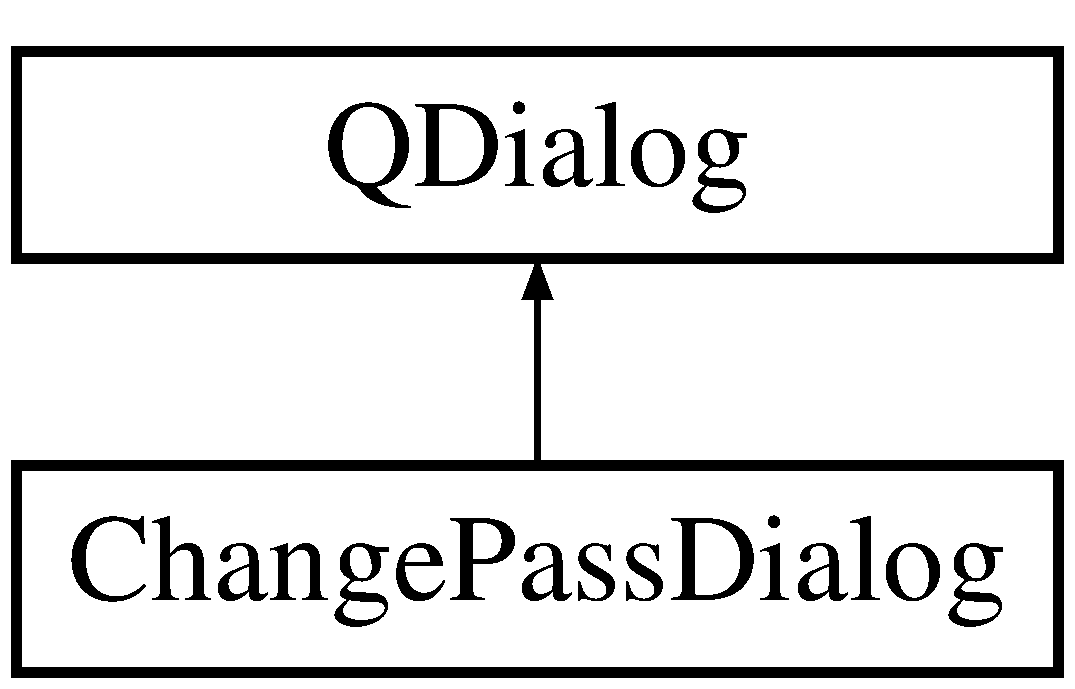
\includegraphics[height=2.000000cm]{class_change_pass_dialog}
\end{center}
\end{figure}
\subsection*{Public Member Functions}
\begin{DoxyCompactItemize}
\item 
\hypertarget{class_change_pass_dialog_ad6f0b8725148486bd3d3240366d01333}{{\bfseries Change\+Pass\+Dialog} (Q\+Widget $\ast$parent=0)}\label{class_change_pass_dialog_ad6f0b8725148486bd3d3240366d01333}

\item 
void \hyperlink{class_change_pass_dialog_a86889ca01de70686efcfe198d0e96963}{set\+Title} (Q\+String title)
\item 
void \hyperlink{class_change_pass_dialog_a6964624bf760e029877b9c7e25d50d18}{set\+Subtitle} (Q\+String subtitle)
\end{DoxyCompactItemize}
\subsection*{Protected Member Functions}
\begin{DoxyCompactItemize}
\item 
void \hyperlink{class_change_pass_dialog_ab086e0854e5e5f15b810ad09f9b18b91}{close\+Event} (Q\+Close\+Event $\ast$event)
\end{DoxyCompactItemize}


\subsection{Detailed Description}
A dialog for changing or entering a new password 

\subsection{Member Function Documentation}
\hypertarget{class_change_pass_dialog_ab086e0854e5e5f15b810ad09f9b18b91}{\index{Change\+Pass\+Dialog@{Change\+Pass\+Dialog}!close\+Event@{close\+Event}}
\index{close\+Event@{close\+Event}!Change\+Pass\+Dialog@{Change\+Pass\+Dialog}}
\subsubsection[{close\+Event}]{\setlength{\rightskip}{0pt plus 5cm}void Change\+Pass\+Dialog\+::close\+Event (
\begin{DoxyParamCaption}
\item[{Q\+Close\+Event $\ast$}]{event}
\end{DoxyParamCaption}
)\hspace{0.3cm}{\ttfamily [protected]}}}\label{class_change_pass_dialog_ab086e0854e5e5f15b810ad09f9b18b91}
Called when close button is pressed \hypertarget{class_change_pass_dialog_a6964624bf760e029877b9c7e25d50d18}{\index{Change\+Pass\+Dialog@{Change\+Pass\+Dialog}!set\+Subtitle@{set\+Subtitle}}
\index{set\+Subtitle@{set\+Subtitle}!Change\+Pass\+Dialog@{Change\+Pass\+Dialog}}
\subsubsection[{set\+Subtitle}]{\setlength{\rightskip}{0pt plus 5cm}void Change\+Pass\+Dialog\+::set\+Subtitle (
\begin{DoxyParamCaption}
\item[{Q\+String}]{subtitle}
\end{DoxyParamCaption}
)}}\label{class_change_pass_dialog_a6964624bf760e029877b9c7e25d50d18}
Set dialog subtitle \hypertarget{class_change_pass_dialog_a86889ca01de70686efcfe198d0e96963}{\index{Change\+Pass\+Dialog@{Change\+Pass\+Dialog}!set\+Title@{set\+Title}}
\index{set\+Title@{set\+Title}!Change\+Pass\+Dialog@{Change\+Pass\+Dialog}}
\subsubsection[{set\+Title}]{\setlength{\rightskip}{0pt plus 5cm}void Change\+Pass\+Dialog\+::set\+Title (
\begin{DoxyParamCaption}
\item[{Q\+String}]{title}
\end{DoxyParamCaption}
)}}\label{class_change_pass_dialog_a86889ca01de70686efcfe198d0e96963}
Set dialog title 

The documentation for this class was generated from the following files\+:\begin{DoxyCompactItemize}
\item 
U\+I/changepassdialog.\+h\item 
U\+I/changepassdialog.\+cpp\end{DoxyCompactItemize}

\hypertarget{class_leap_1_1_circle_gesture}{\section{Leap\+:\+:Circle\+Gesture Class Reference}
\label{class_leap_1_1_circle_gesture}\index{Leap\+::\+Circle\+Gesture@{Leap\+::\+Circle\+Gesture}}
}


{\ttfamily \#include $<$Leap.\+h$>$}

Inheritance diagram for Leap\+:\+:Circle\+Gesture\+:\begin{figure}[H]
\begin{center}
\leavevmode
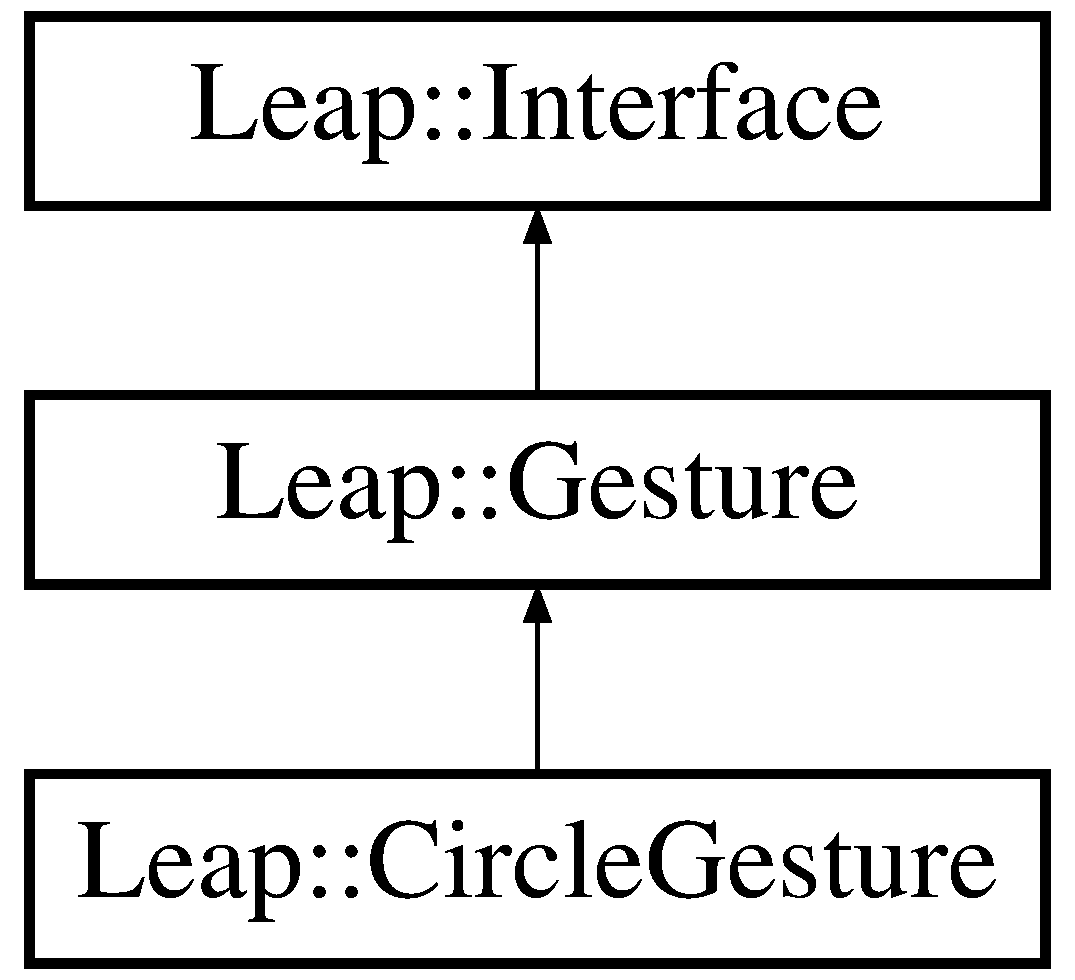
\includegraphics[height=3.000000cm]{class_leap_1_1_circle_gesture}
\end{center}
\end{figure}
\subsection*{Public Member Functions}
\begin{DoxyCompactItemize}
\item 
L\+E\+A\+P\+\_\+\+E\+X\+P\+O\+R\+T \hyperlink{class_leap_1_1_circle_gesture_a67ac2907b68958693129eb7a6f731722}{Circle\+Gesture} ()
\item 
L\+E\+A\+P\+\_\+\+E\+X\+P\+O\+R\+T \hyperlink{class_leap_1_1_circle_gesture_a3a27444e1657e1ecf3e74bc9c7cad292}{Circle\+Gesture} (const \hyperlink{class_leap_1_1_gesture}{Gesture} \&rhs)
\item 
L\+E\+A\+P\+\_\+\+E\+X\+P\+O\+R\+T \hyperlink{struct_leap_1_1_vector}{Vector} \hyperlink{class_leap_1_1_circle_gesture_aa6f358e771078c056dea579511707784}{center} () const 
\item 
L\+E\+A\+P\+\_\+\+E\+X\+P\+O\+R\+T \hyperlink{struct_leap_1_1_vector}{Vector} \hyperlink{class_leap_1_1_circle_gesture_ae0fbdb4a8905e289afa885c2f304ae52}{normal} () const 
\item 
L\+E\+A\+P\+\_\+\+E\+X\+P\+O\+R\+T float \hyperlink{class_leap_1_1_circle_gesture_a6117b3ab528b6af6ae2d76b1afa03110}{progress} () const 
\item 
L\+E\+A\+P\+\_\+\+E\+X\+P\+O\+R\+T float \hyperlink{class_leap_1_1_circle_gesture_a25b6f377b953f82c4d0c2a7488c02253}{radius} () const 
\item 
L\+E\+A\+P\+\_\+\+E\+X\+P\+O\+R\+T \hyperlink{class_leap_1_1_pointable}{Pointable} \hyperlink{class_leap_1_1_circle_gesture_adc211d647af2a5853773dbabf5deb1ab}{pointable} () const 
\end{DoxyCompactItemize}
\subsection*{Static Public Member Functions}
\begin{DoxyCompactItemize}
\item 
static \hyperlink{class_leap_1_1_gesture_a6fa6dd4f28c502f0d55abc6b71c6f9b1}{Type} \hyperlink{class_leap_1_1_circle_gesture_a8935a8a71b0a174a1656ff2caab80a06}{class\+Type} ()
\end{DoxyCompactItemize}
\subsection*{Additional Inherited Members}


\subsection{Detailed Description}
The \hyperlink{class_leap_1_1_circle_gesture}{Circle\+Gesture} classes represents a circular finger movement.

A circle movement is recognized when the tip of a finger draws a circle within the Leap Motion \hyperlink{class_leap_1_1_controller}{Controller} field of view.



{\bfseries Important\+:} To use circle gestures in your application, you must enable recognition of the circle gesture. You can enable recognition with\+:


\begin{DoxyCodeInclude}
\end{DoxyCodeInclude}


Circle gestures are continuous. The \hyperlink{class_leap_1_1_circle_gesture}{Circle\+Gesture} objects for the gesture have three possible states\+:


\begin{DoxyItemize}
\item State\+::\+S\+T\+A\+T\+E\+\_\+\+S\+T\+A\+R\+T -- The circle gesture has just started. The movement has progressed far enough for the recognizer to classify it as a circle.
\item State\+::\+S\+T\+A\+T\+E\+\_\+\+U\+P\+D\+A\+T\+E -- The circle gesture is continuing.
\item State\+::\+S\+T\+A\+T\+E\+\_\+\+S\+T\+O\+P -- The circle gesture is finished.
\end{DoxyItemize}

You can set the minimum radius and minimum arc length required for a movement to be recognized as a circle using the config attribute of a connected \hyperlink{class_leap_1_1_controller}{Controller} object. Use the following keys to configure circle recognition\+:

\begin{TabularC}{4}
\hline
\rowcolor{lightgray}{\bf Key string }&{\bf Value type }&{\bf Default value }&{\bf Units  }\\\cline{1-4}
Gesture.\+Circle.\+Min\+Radius &float &5.\+0 &mm \\\cline{1-4}
Gesture.\+Circle.\+Min\+Arc &float &1.\+5$\ast$pi &radians \\\cline{1-4}
\end{TabularC}
The following example demonstrates how to set the circle configuration parameters\+:


\begin{DoxyCodeInclude}
\end{DoxyCodeInclude}
 \begin{DoxySince}{Since}
1.\+0 
\end{DoxySince}


\subsection{Constructor \& Destructor Documentation}
\hypertarget{class_leap_1_1_circle_gesture_a67ac2907b68958693129eb7a6f731722}{\index{Leap\+::\+Circle\+Gesture@{Leap\+::\+Circle\+Gesture}!Circle\+Gesture@{Circle\+Gesture}}
\index{Circle\+Gesture@{Circle\+Gesture}!Leap\+::\+Circle\+Gesture@{Leap\+::\+Circle\+Gesture}}
\subsubsection[{Circle\+Gesture}]{\setlength{\rightskip}{0pt plus 5cm}L\+E\+A\+P\+\_\+\+E\+X\+P\+O\+R\+T Leap\+::\+Circle\+Gesture\+::\+Circle\+Gesture (
\begin{DoxyParamCaption}
{}
\end{DoxyParamCaption}
)}}\label{class_leap_1_1_circle_gesture_a67ac2907b68958693129eb7a6f731722}
Constructs a new \hyperlink{class_leap_1_1_circle_gesture}{Circle\+Gesture} object.

An uninitialized \hyperlink{class_leap_1_1_circle_gesture}{Circle\+Gesture} object is considered invalid. Get valid instances of the \hyperlink{class_leap_1_1_circle_gesture}{Circle\+Gesture} class from a \hyperlink{class_leap_1_1_frame}{Frame} object. \begin{DoxySince}{Since}
1.\+0 
\end{DoxySince}
\hypertarget{class_leap_1_1_circle_gesture_a3a27444e1657e1ecf3e74bc9c7cad292}{\index{Leap\+::\+Circle\+Gesture@{Leap\+::\+Circle\+Gesture}!Circle\+Gesture@{Circle\+Gesture}}
\index{Circle\+Gesture@{Circle\+Gesture}!Leap\+::\+Circle\+Gesture@{Leap\+::\+Circle\+Gesture}}
\subsubsection[{Circle\+Gesture}]{\setlength{\rightskip}{0pt plus 5cm}L\+E\+A\+P\+\_\+\+E\+X\+P\+O\+R\+T Leap\+::\+Circle\+Gesture\+::\+Circle\+Gesture (
\begin{DoxyParamCaption}
\item[{const {\bf Gesture} \&}]{rhs}
\end{DoxyParamCaption}
)}}\label{class_leap_1_1_circle_gesture_a3a27444e1657e1ecf3e74bc9c7cad292}
Constructs a \hyperlink{class_leap_1_1_circle_gesture}{Circle\+Gesture} object from an instance of the \hyperlink{class_leap_1_1_gesture}{Gesture} class.


\begin{DoxyParams}{Parameters}
{\em rhs} & The \hyperlink{class_leap_1_1_gesture}{Gesture} instance to specialize. This \hyperlink{class_leap_1_1_gesture}{Gesture} instance must be a \hyperlink{class_leap_1_1_circle_gesture}{Circle\+Gesture} object. \\
\hline
\end{DoxyParams}
\begin{DoxySince}{Since}
1.\+0 
\end{DoxySince}


\subsection{Member Function Documentation}
\hypertarget{class_leap_1_1_circle_gesture_aa6f358e771078c056dea579511707784}{\index{Leap\+::\+Circle\+Gesture@{Leap\+::\+Circle\+Gesture}!center@{center}}
\index{center@{center}!Leap\+::\+Circle\+Gesture@{Leap\+::\+Circle\+Gesture}}
\subsubsection[{center}]{\setlength{\rightskip}{0pt plus 5cm}L\+E\+A\+P\+\_\+\+E\+X\+P\+O\+R\+T {\bf Vector} Leap\+::\+Circle\+Gesture\+::center (
\begin{DoxyParamCaption}
{}
\end{DoxyParamCaption}
) const}}\label{class_leap_1_1_circle_gesture_aa6f358e771078c056dea579511707784}
The center point of the circle within the Leap Motion frame of reference.

\begin{DoxyReturn}{Returns}
\hyperlink{struct_leap_1_1_vector}{Vector} The center of the circle in mm from the Leap Motion origin. 
\end{DoxyReturn}
\begin{DoxySince}{Since}
1.\+0 
\end{DoxySince}
\hypertarget{class_leap_1_1_circle_gesture_a8935a8a71b0a174a1656ff2caab80a06}{\index{Leap\+::\+Circle\+Gesture@{Leap\+::\+Circle\+Gesture}!class\+Type@{class\+Type}}
\index{class\+Type@{class\+Type}!Leap\+::\+Circle\+Gesture@{Leap\+::\+Circle\+Gesture}}
\subsubsection[{class\+Type}]{\setlength{\rightskip}{0pt plus 5cm}static {\bf Type} Leap\+::\+Circle\+Gesture\+::class\+Type (
\begin{DoxyParamCaption}
{}
\end{DoxyParamCaption}
)\hspace{0.3cm}{\ttfamily [inline]}, {\ttfamily [static]}}}\label{class_leap_1_1_circle_gesture_a8935a8a71b0a174a1656ff2caab80a06}
The circle gesture type.

\begin{DoxyReturn}{Returns}
Type The type value designating a circle gesture. 
\end{DoxyReturn}
\begin{DoxySince}{Since}
1.\+0 
\end{DoxySince}
\hypertarget{class_leap_1_1_circle_gesture_ae0fbdb4a8905e289afa885c2f304ae52}{\index{Leap\+::\+Circle\+Gesture@{Leap\+::\+Circle\+Gesture}!normal@{normal}}
\index{normal@{normal}!Leap\+::\+Circle\+Gesture@{Leap\+::\+Circle\+Gesture}}
\subsubsection[{normal}]{\setlength{\rightskip}{0pt plus 5cm}L\+E\+A\+P\+\_\+\+E\+X\+P\+O\+R\+T {\bf Vector} Leap\+::\+Circle\+Gesture\+::normal (
\begin{DoxyParamCaption}
{}
\end{DoxyParamCaption}
) const}}\label{class_leap_1_1_circle_gesture_ae0fbdb4a8905e289afa885c2f304ae52}
Returns the normal vector for the circle being traced.

If you draw the circle clockwise, the normal vector points in the same general direction as the pointable object drawing the circle. If you draw the circle counterclockwise, the normal points back toward the pointable. If the angle between the normal and the pointable object drawing the circle is less than 90 degrees, then the circle is clockwise.


\begin{DoxyCodeInclude}
\end{DoxyCodeInclude}


\begin{DoxyReturn}{Returns}
\hyperlink{struct_leap_1_1_vector}{Vector} the normal vector for the circle being traced 
\end{DoxyReturn}
\begin{DoxySince}{Since}
1.\+0 
\end{DoxySince}
\hypertarget{class_leap_1_1_circle_gesture_adc211d647af2a5853773dbabf5deb1ab}{\index{Leap\+::\+Circle\+Gesture@{Leap\+::\+Circle\+Gesture}!pointable@{pointable}}
\index{pointable@{pointable}!Leap\+::\+Circle\+Gesture@{Leap\+::\+Circle\+Gesture}}
\subsubsection[{pointable}]{\setlength{\rightskip}{0pt plus 5cm}L\+E\+A\+P\+\_\+\+E\+X\+P\+O\+R\+T {\bf Pointable} Leap\+::\+Circle\+Gesture\+::pointable (
\begin{DoxyParamCaption}
{}
\end{DoxyParamCaption}
) const}}\label{class_leap_1_1_circle_gesture_adc211d647af2a5853773dbabf5deb1ab}
The finger performing the circle gesture.

\begin{DoxyReturn}{Returns}
\hyperlink{class_leap_1_1_pointable}{Pointable} A \hyperlink{class_leap_1_1_pointable}{Pointable} object representing the circling finger. 
\end{DoxyReturn}
\begin{DoxySince}{Since}
1.\+0 
\end{DoxySince}
\hypertarget{class_leap_1_1_circle_gesture_a6117b3ab528b6af6ae2d76b1afa03110}{\index{Leap\+::\+Circle\+Gesture@{Leap\+::\+Circle\+Gesture}!progress@{progress}}
\index{progress@{progress}!Leap\+::\+Circle\+Gesture@{Leap\+::\+Circle\+Gesture}}
\subsubsection[{progress}]{\setlength{\rightskip}{0pt plus 5cm}L\+E\+A\+P\+\_\+\+E\+X\+P\+O\+R\+T float Leap\+::\+Circle\+Gesture\+::progress (
\begin{DoxyParamCaption}
{}
\end{DoxyParamCaption}
) const}}\label{class_leap_1_1_circle_gesture_a6117b3ab528b6af6ae2d76b1afa03110}
The number of times the finger tip has traversed the circle.

Progress is reported as a positive number of the number. For example, a progress value of .5 indicates that the finger has gone halfway around, while a value of 3 indicates that the finger has gone around the the circle three times.

Progress starts where the circle gesture began. Since the circle must be partially formed before the Leap Motion software can recognize it, progress will be greater than zero when a circle gesture first appears in the frame.

\begin{DoxyReturn}{Returns}
float A positive number indicating the gesture progress. 
\end{DoxyReturn}
\begin{DoxySince}{Since}
1.\+0 
\end{DoxySince}
\hypertarget{class_leap_1_1_circle_gesture_a25b6f377b953f82c4d0c2a7488c02253}{\index{Leap\+::\+Circle\+Gesture@{Leap\+::\+Circle\+Gesture}!radius@{radius}}
\index{radius@{radius}!Leap\+::\+Circle\+Gesture@{Leap\+::\+Circle\+Gesture}}
\subsubsection[{radius}]{\setlength{\rightskip}{0pt plus 5cm}L\+E\+A\+P\+\_\+\+E\+X\+P\+O\+R\+T float Leap\+::\+Circle\+Gesture\+::radius (
\begin{DoxyParamCaption}
{}
\end{DoxyParamCaption}
) const}}\label{class_leap_1_1_circle_gesture_a25b6f377b953f82c4d0c2a7488c02253}
The radius of the circle.

\begin{DoxyReturn}{Returns}
The circle radius in mm. 
\end{DoxyReturn}
\begin{DoxySince}{Since}
1.\+0 
\end{DoxySince}


The documentation for this class was generated from the following file\+:\begin{DoxyCompactItemize}
\item 
Interface\+Managers/Leap.\+h\end{DoxyCompactItemize}

\hypertarget{class_leap_1_1_config}{\section{Leap\+:\+:Config Class Reference}
\label{class_leap_1_1_config}\index{Leap\+::\+Config@{Leap\+::\+Config}}
}


{\ttfamily \#include $<$Leap.\+h$>$}

Inheritance diagram for Leap\+:\+:Config\+:\begin{figure}[H]
\begin{center}
\leavevmode
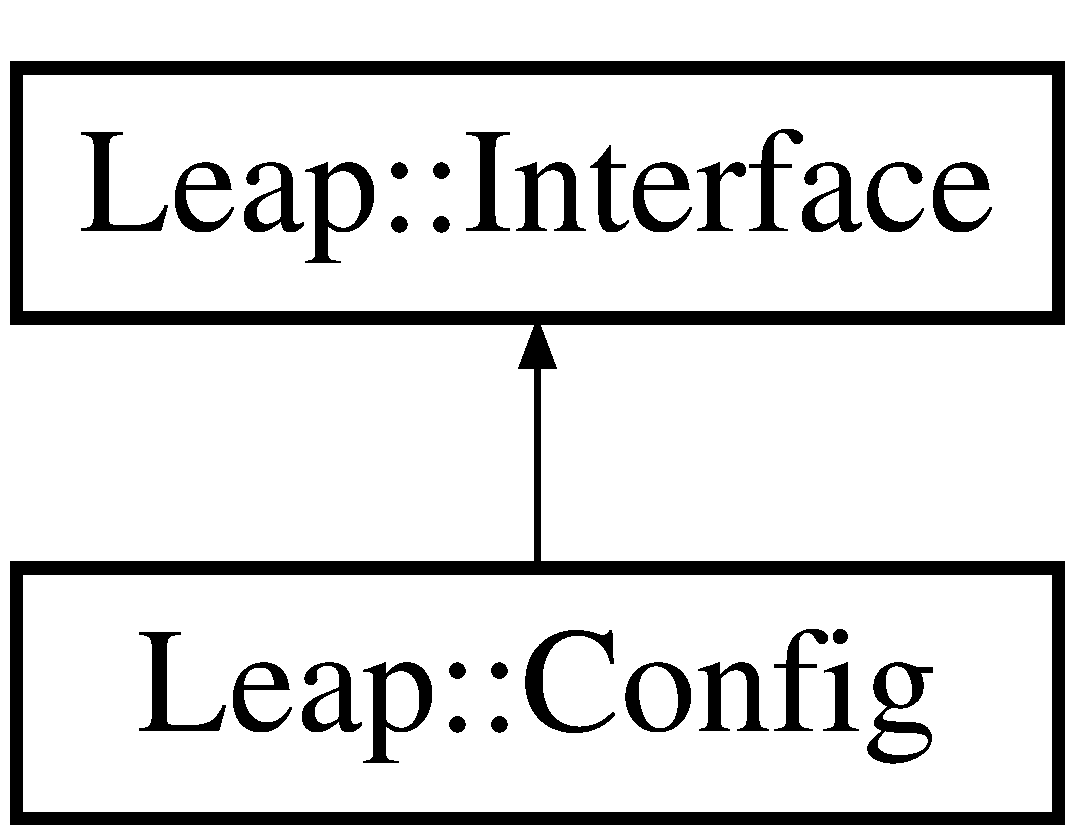
\includegraphics[height=2.000000cm]{class_leap_1_1_config}
\end{center}
\end{figure}
\subsection*{Public Types}
\begin{DoxyCompactItemize}
\item 
enum \hyperlink{class_leap_1_1_config_aee9819af7eacacc324aa72619310a9d8}{Value\+Type} \{ \\*
\hyperlink{class_leap_1_1_config_aee9819af7eacacc324aa72619310a9d8a61027e87139ecf1153e7b7f41fd9adfa}{T\+Y\+P\+E\+\_\+\+U\+N\+K\+N\+O\+W\+N} = 0, 
\hyperlink{class_leap_1_1_config_aee9819af7eacacc324aa72619310a9d8a592e8eabddb7d95b192fee923c423760}{T\+Y\+P\+E\+\_\+\+B\+O\+O\+L\+E\+A\+N} = 1, 
\hyperlink{class_leap_1_1_config_aee9819af7eacacc324aa72619310a9d8af552faf6063e26e0b5a995c344cfaebd}{T\+Y\+P\+E\+\_\+\+I\+N\+T32} = 2, 
\hyperlink{class_leap_1_1_config_aee9819af7eacacc324aa72619310a9d8a85ccbf5a55972697b350b394f7d87cfa}{T\+Y\+P\+E\+\_\+\+F\+L\+O\+A\+T} = 6, 
\\*
\hyperlink{class_leap_1_1_config_aee9819af7eacacc324aa72619310a9d8a312ad72cfe51163b2817732f7530e04e}{T\+Y\+P\+E\+\_\+\+S\+T\+R\+I\+N\+G} = 8
 \}
\end{DoxyCompactItemize}
\subsection*{Public Member Functions}
\begin{DoxyCompactItemize}
\item 
L\+E\+A\+P\+\_\+\+E\+X\+P\+O\+R\+T \hyperlink{class_leap_1_1_config_aee58922e575e3e59ddf8da5af4f07878}{Config} ()
\item 
L\+E\+A\+P\+\_\+\+E\+X\+P\+O\+R\+T \hyperlink{class_leap_1_1_config_aee9819af7eacacc324aa72619310a9d8}{Value\+Type} \hyperlink{class_leap_1_1_config_ac5ed7b7b0562cc4dae2d0b4ab8187b12}{type} (const std\+::string \&key) const 
\item 
L\+E\+A\+P\+\_\+\+E\+X\+P\+O\+R\+T bool \hyperlink{class_leap_1_1_config_a52200e2fe5473caf1c0dbc91e0733c0c}{get\+Bool} (const std\+::string \&key) const 
\item 
L\+E\+A\+P\+\_\+\+E\+X\+P\+O\+R\+T bool \hyperlink{class_leap_1_1_config_ac6a084454142d87f1662b3b279dfe9e9}{set\+Bool} (const std\+::string \&key, bool value)
\item 
L\+E\+A\+P\+\_\+\+E\+X\+P\+O\+R\+T int32\+\_\+t \hyperlink{class_leap_1_1_config_a135ebf47e6a3a803527a7cc035029cb0}{get\+Int32} (const std\+::string \&key) const 
\item 
L\+E\+A\+P\+\_\+\+E\+X\+P\+O\+R\+T bool \hyperlink{class_leap_1_1_config_a47d811c2727695ecd1916e313b54736c}{set\+Int32} (const std\+::string \&key, int32\+\_\+t value)
\item 
L\+E\+A\+P\+\_\+\+E\+X\+P\+O\+R\+T float \hyperlink{class_leap_1_1_config_ace93b634211d8cf237c9d40a2e497b44}{get\+Float} (const std\+::string \&key) const 
\item 
L\+E\+A\+P\+\_\+\+E\+X\+P\+O\+R\+T bool \hyperlink{class_leap_1_1_config_a6d9442a88f622b00f9c432c4ac9b7c35}{set\+Float} (const std\+::string \&key, float value)
\item 
L\+E\+A\+P\+\_\+\+E\+X\+P\+O\+R\+T std\+::string \hyperlink{class_leap_1_1_config_a4b408ca65a8b7064733e26be93af3f2d}{get\+String} (const std\+::string \&key) const 
\item 
L\+E\+A\+P\+\_\+\+E\+X\+P\+O\+R\+T bool \hyperlink{class_leap_1_1_config_a5cd3b0eaf702cc304071c244a52b3bed}{set\+String} (const std\+::string \&key, const std\+::string \&value)
\item 
L\+E\+A\+P\+\_\+\+E\+X\+P\+O\+R\+T bool \hyperlink{class_leap_1_1_config_ae1187e2b9992706d2a3eb071cc2f71c4}{save} ()
\end{DoxyCompactItemize}
\subsection*{Additional Inherited Members}


\subsection{Detailed Description}
The \hyperlink{class_leap_1_1_config}{Config} class provides access to Leap Motion system configuration information.

You can get and set gesture configuration parameters using the \hyperlink{class_leap_1_1_config}{Config} object obtained from a connected \hyperlink{class_leap_1_1_controller}{Controller} object. The key strings required to identify a configuration parameter include\+:

\begin{TabularC}{4}
\hline
\rowcolor{lightgray}{\bf Key string }&{\bf Value type }&{\bf Default value }&{\bf Units  }\\\cline{1-4}
Gesture.\+Circle.\+Min\+Radius &float &5.\+0 &mm \\\cline{1-4}
Gesture.\+Circle.\+Min\+Arc &float &1.\+5$\ast$pi &radians \\\cline{1-4}
Gesture.\+Swipe.\+Min\+Length &float &150 &mm \\\cline{1-4}
Gesture.\+Swipe.\+Min\+Velocity &float &1000 &mm/s \\\cline{1-4}
Gesture.\+Key\+Tap.\+Min\+Down\+Velocity &float &50 &mm/s \\\cline{1-4}
Gesture.\+Key\+Tap.\+History\+Seconds &float &0.\+1 &s \\\cline{1-4}
Gesture.\+Key\+Tap.\+Min\+Distance &float &3.\+0 &mm \\\cline{1-4}
Gesture.\+Screen\+Tap.\+Min\+Forward\+Velocity &float &50 &mm/s \\\cline{1-4}
Gesture.\+Screen\+Tap.\+History\+Seconds &float &0.\+1 &s \\\cline{1-4}
Gesture.\+Screen\+Tap.\+Min\+Distance &float &5.\+0 &mm \\\cline{1-4}
\end{TabularC}
After setting a configuration value, you must call the \hyperlink{class_leap_1_1_config_ae1187e2b9992706d2a3eb071cc2f71c4}{Config\+::save} method to commit the changes. The configuration value changes are not persistent; your application needs to set the values everytime it runs.

\begin{DoxySeeAlso}{See also}
\hyperlink{class_leap_1_1_circle_gesture}{Circle\+Gesture} 

\hyperlink{class_leap_1_1_key_tap_gesture}{Key\+Tap\+Gesture} 

\hyperlink{class_leap_1_1_screen_tap_gesture}{Screen\+Tap\+Gesture} 

\hyperlink{class_leap_1_1_swipe_gesture}{Swipe\+Gesture} 
\end{DoxySeeAlso}
\begin{DoxySince}{Since}
1.\+0 
\end{DoxySince}


\subsection{Member Enumeration Documentation}
\hypertarget{class_leap_1_1_config_aee9819af7eacacc324aa72619310a9d8}{\index{Leap\+::\+Config@{Leap\+::\+Config}!Value\+Type@{Value\+Type}}
\index{Value\+Type@{Value\+Type}!Leap\+::\+Config@{Leap\+::\+Config}}
\subsubsection[{Value\+Type}]{\setlength{\rightskip}{0pt plus 5cm}enum {\bf Leap\+::\+Config\+::\+Value\+Type}}}\label{class_leap_1_1_config_aee9819af7eacacc324aa72619310a9d8}
Enumerates the possible data types for configuration values.

The \hyperlink{class_leap_1_1_config_ac5ed7b7b0562cc4dae2d0b4ab8187b12}{Config\+::type()} function returns an item from the Value\+Type enumeration. \begin{DoxySince}{Since}
1.\+0 
\end{DoxySince}
\begin{Desc}
\item[Enumerator]\par
\begin{description}
\index{T\+Y\+P\+E\+\_\+\+U\+N\+K\+N\+O\+W\+N@{T\+Y\+P\+E\+\_\+\+U\+N\+K\+N\+O\+W\+N}!Leap\+::\+Config@{Leap\+::\+Config}}\index{Leap\+::\+Config@{Leap\+::\+Config}!T\+Y\+P\+E\+\_\+\+U\+N\+K\+N\+O\+W\+N@{T\+Y\+P\+E\+\_\+\+U\+N\+K\+N\+O\+W\+N}}\item[{\em 
\hypertarget{class_leap_1_1_config_aee9819af7eacacc324aa72619310a9d8a61027e87139ecf1153e7b7f41fd9adfa}{T\+Y\+P\+E\+\_\+\+U\+N\+K\+N\+O\+W\+N}\label{class_leap_1_1_config_aee9819af7eacacc324aa72619310a9d8a61027e87139ecf1153e7b7f41fd9adfa}
}]The data type is unknown. \begin{DoxySince}{Since}
1.\+0 
\end{DoxySince}
\index{T\+Y\+P\+E\+\_\+\+B\+O\+O\+L\+E\+A\+N@{T\+Y\+P\+E\+\_\+\+B\+O\+O\+L\+E\+A\+N}!Leap\+::\+Config@{Leap\+::\+Config}}\index{Leap\+::\+Config@{Leap\+::\+Config}!T\+Y\+P\+E\+\_\+\+B\+O\+O\+L\+E\+A\+N@{T\+Y\+P\+E\+\_\+\+B\+O\+O\+L\+E\+A\+N}}\item[{\em 
\hypertarget{class_leap_1_1_config_aee9819af7eacacc324aa72619310a9d8a592e8eabddb7d95b192fee923c423760}{T\+Y\+P\+E\+\_\+\+B\+O\+O\+L\+E\+A\+N}\label{class_leap_1_1_config_aee9819af7eacacc324aa72619310a9d8a592e8eabddb7d95b192fee923c423760}
}]A boolean value. \begin{DoxySince}{Since}
1.\+0 
\end{DoxySince}
\index{T\+Y\+P\+E\+\_\+\+I\+N\+T32@{T\+Y\+P\+E\+\_\+\+I\+N\+T32}!Leap\+::\+Config@{Leap\+::\+Config}}\index{Leap\+::\+Config@{Leap\+::\+Config}!T\+Y\+P\+E\+\_\+\+I\+N\+T32@{T\+Y\+P\+E\+\_\+\+I\+N\+T32}}\item[{\em 
\hypertarget{class_leap_1_1_config_aee9819af7eacacc324aa72619310a9d8af552faf6063e26e0b5a995c344cfaebd}{T\+Y\+P\+E\+\_\+\+I\+N\+T32}\label{class_leap_1_1_config_aee9819af7eacacc324aa72619310a9d8af552faf6063e26e0b5a995c344cfaebd}
}]A 32-\/bit integer. \begin{DoxySince}{Since}
1.\+0 
\end{DoxySince}
\index{T\+Y\+P\+E\+\_\+\+F\+L\+O\+A\+T@{T\+Y\+P\+E\+\_\+\+F\+L\+O\+A\+T}!Leap\+::\+Config@{Leap\+::\+Config}}\index{Leap\+::\+Config@{Leap\+::\+Config}!T\+Y\+P\+E\+\_\+\+F\+L\+O\+A\+T@{T\+Y\+P\+E\+\_\+\+F\+L\+O\+A\+T}}\item[{\em 
\hypertarget{class_leap_1_1_config_aee9819af7eacacc324aa72619310a9d8a85ccbf5a55972697b350b394f7d87cfa}{T\+Y\+P\+E\+\_\+\+F\+L\+O\+A\+T}\label{class_leap_1_1_config_aee9819af7eacacc324aa72619310a9d8a85ccbf5a55972697b350b394f7d87cfa}
}]A floating-\/point number. \begin{DoxySince}{Since}
1.\+0 
\end{DoxySince}
\index{T\+Y\+P\+E\+\_\+\+S\+T\+R\+I\+N\+G@{T\+Y\+P\+E\+\_\+\+S\+T\+R\+I\+N\+G}!Leap\+::\+Config@{Leap\+::\+Config}}\index{Leap\+::\+Config@{Leap\+::\+Config}!T\+Y\+P\+E\+\_\+\+S\+T\+R\+I\+N\+G@{T\+Y\+P\+E\+\_\+\+S\+T\+R\+I\+N\+G}}\item[{\em 
\hypertarget{class_leap_1_1_config_aee9819af7eacacc324aa72619310a9d8a312ad72cfe51163b2817732f7530e04e}{T\+Y\+P\+E\+\_\+\+S\+T\+R\+I\+N\+G}\label{class_leap_1_1_config_aee9819af7eacacc324aa72619310a9d8a312ad72cfe51163b2817732f7530e04e}
}]A string of characters. \begin{DoxySince}{Since}
1.\+0 
\end{DoxySince}
\end{description}
\end{Desc}


\subsection{Constructor \& Destructor Documentation}
\hypertarget{class_leap_1_1_config_aee58922e575e3e59ddf8da5af4f07878}{\index{Leap\+::\+Config@{Leap\+::\+Config}!Config@{Config}}
\index{Config@{Config}!Leap\+::\+Config@{Leap\+::\+Config}}
\subsubsection[{Config}]{\setlength{\rightskip}{0pt plus 5cm}L\+E\+A\+P\+\_\+\+E\+X\+P\+O\+R\+T Leap\+::\+Config\+::\+Config (
\begin{DoxyParamCaption}
{}
\end{DoxyParamCaption}
)}}\label{class_leap_1_1_config_aee58922e575e3e59ddf8da5af4f07878}
Constructs a \hyperlink{class_leap_1_1_config}{Config} object. \begin{DoxySince}{Since}
1.\+0 
\end{DoxySince}


\subsection{Member Function Documentation}
\hypertarget{class_leap_1_1_config_a52200e2fe5473caf1c0dbc91e0733c0c}{\index{Leap\+::\+Config@{Leap\+::\+Config}!get\+Bool@{get\+Bool}}
\index{get\+Bool@{get\+Bool}!Leap\+::\+Config@{Leap\+::\+Config}}
\subsubsection[{get\+Bool}]{\setlength{\rightskip}{0pt plus 5cm}L\+E\+A\+P\+\_\+\+E\+X\+P\+O\+R\+T bool Leap\+::\+Config\+::get\+Bool (
\begin{DoxyParamCaption}
\item[{const std\+::string \&}]{key}
\end{DoxyParamCaption}
) const}}\label{class_leap_1_1_config_a52200e2fe5473caf1c0dbc91e0733c0c}
Gets the boolean representation for the specified key. \begin{DoxySince}{Since}
1.\+0 
\end{DoxySince}
\hypertarget{class_leap_1_1_config_ace93b634211d8cf237c9d40a2e497b44}{\index{Leap\+::\+Config@{Leap\+::\+Config}!get\+Float@{get\+Float}}
\index{get\+Float@{get\+Float}!Leap\+::\+Config@{Leap\+::\+Config}}
\subsubsection[{get\+Float}]{\setlength{\rightskip}{0pt plus 5cm}L\+E\+A\+P\+\_\+\+E\+X\+P\+O\+R\+T float Leap\+::\+Config\+::get\+Float (
\begin{DoxyParamCaption}
\item[{const std\+::string \&}]{key}
\end{DoxyParamCaption}
) const}}\label{class_leap_1_1_config_ace93b634211d8cf237c9d40a2e497b44}
Gets the floating point representation for the specified key. \begin{DoxySince}{Since}
1.\+0 
\end{DoxySince}
\hypertarget{class_leap_1_1_config_a135ebf47e6a3a803527a7cc035029cb0}{\index{Leap\+::\+Config@{Leap\+::\+Config}!get\+Int32@{get\+Int32}}
\index{get\+Int32@{get\+Int32}!Leap\+::\+Config@{Leap\+::\+Config}}
\subsubsection[{get\+Int32}]{\setlength{\rightskip}{0pt plus 5cm}L\+E\+A\+P\+\_\+\+E\+X\+P\+O\+R\+T int32\+\_\+t Leap\+::\+Config\+::get\+Int32 (
\begin{DoxyParamCaption}
\item[{const std\+::string \&}]{key}
\end{DoxyParamCaption}
) const}}\label{class_leap_1_1_config_a135ebf47e6a3a803527a7cc035029cb0}
Gets the 32-\/bit integer representation for the specified key. \begin{DoxySince}{Since}
1.\+0 
\end{DoxySince}
\hypertarget{class_leap_1_1_config_a4b408ca65a8b7064733e26be93af3f2d}{\index{Leap\+::\+Config@{Leap\+::\+Config}!get\+String@{get\+String}}
\index{get\+String@{get\+String}!Leap\+::\+Config@{Leap\+::\+Config}}
\subsubsection[{get\+String}]{\setlength{\rightskip}{0pt plus 5cm}L\+E\+A\+P\+\_\+\+E\+X\+P\+O\+R\+T std\+::string Leap\+::\+Config\+::get\+String (
\begin{DoxyParamCaption}
\item[{const std\+::string \&}]{key}
\end{DoxyParamCaption}
) const}}\label{class_leap_1_1_config_a4b408ca65a8b7064733e26be93af3f2d}
Gets the string representation for the specified key. \begin{DoxySince}{Since}
1.\+0 
\end{DoxySince}
\hypertarget{class_leap_1_1_config_ae1187e2b9992706d2a3eb071cc2f71c4}{\index{Leap\+::\+Config@{Leap\+::\+Config}!save@{save}}
\index{save@{save}!Leap\+::\+Config@{Leap\+::\+Config}}
\subsubsection[{save}]{\setlength{\rightskip}{0pt plus 5cm}L\+E\+A\+P\+\_\+\+E\+X\+P\+O\+R\+T bool Leap\+::\+Config\+::save (
\begin{DoxyParamCaption}
{}
\end{DoxyParamCaption}
)}}\label{class_leap_1_1_config_ae1187e2b9992706d2a3eb071cc2f71c4}
Saves the current state of the config.

Call {\ttfamily \hyperlink{class_leap_1_1_config_ae1187e2b9992706d2a3eb071cc2f71c4}{save()}} after making a set of configuration changes. The {\ttfamily \hyperlink{class_leap_1_1_config_ae1187e2b9992706d2a3eb071cc2f71c4}{save()}} function transfers the configuration changes to the Leap Motion service. The configuration value changes are not persistent; your application must set the values everytime it runs.

\begin{DoxyReturn}{Returns}
true on success, false on failure. 
\end{DoxyReturn}
\begin{DoxySince}{Since}
1.\+0 
\end{DoxySince}
\hypertarget{class_leap_1_1_config_ac6a084454142d87f1662b3b279dfe9e9}{\index{Leap\+::\+Config@{Leap\+::\+Config}!set\+Bool@{set\+Bool}}
\index{set\+Bool@{set\+Bool}!Leap\+::\+Config@{Leap\+::\+Config}}
\subsubsection[{set\+Bool}]{\setlength{\rightskip}{0pt plus 5cm}L\+E\+A\+P\+\_\+\+E\+X\+P\+O\+R\+T bool Leap\+::\+Config\+::set\+Bool (
\begin{DoxyParamCaption}
\item[{const std\+::string \&}]{key, }
\item[{bool}]{value}
\end{DoxyParamCaption}
)}}\label{class_leap_1_1_config_ac6a084454142d87f1662b3b279dfe9e9}
Sets the boolean representation for the specified key. \begin{DoxyReturn}{Returns}
true on success, false on failure. 
\end{DoxyReturn}
\begin{DoxySince}{Since}
1.\+0 
\end{DoxySince}
\hypertarget{class_leap_1_1_config_a6d9442a88f622b00f9c432c4ac9b7c35}{\index{Leap\+::\+Config@{Leap\+::\+Config}!set\+Float@{set\+Float}}
\index{set\+Float@{set\+Float}!Leap\+::\+Config@{Leap\+::\+Config}}
\subsubsection[{set\+Float}]{\setlength{\rightskip}{0pt plus 5cm}L\+E\+A\+P\+\_\+\+E\+X\+P\+O\+R\+T bool Leap\+::\+Config\+::set\+Float (
\begin{DoxyParamCaption}
\item[{const std\+::string \&}]{key, }
\item[{float}]{value}
\end{DoxyParamCaption}
)}}\label{class_leap_1_1_config_a6d9442a88f622b00f9c432c4ac9b7c35}
Sets the floating point representation for the specified key. \begin{DoxyReturn}{Returns}
true on success, false on failure. 
\end{DoxyReturn}
\begin{DoxySince}{Since}
1.\+0 
\end{DoxySince}
\hypertarget{class_leap_1_1_config_a47d811c2727695ecd1916e313b54736c}{\index{Leap\+::\+Config@{Leap\+::\+Config}!set\+Int32@{set\+Int32}}
\index{set\+Int32@{set\+Int32}!Leap\+::\+Config@{Leap\+::\+Config}}
\subsubsection[{set\+Int32}]{\setlength{\rightskip}{0pt plus 5cm}L\+E\+A\+P\+\_\+\+E\+X\+P\+O\+R\+T bool Leap\+::\+Config\+::set\+Int32 (
\begin{DoxyParamCaption}
\item[{const std\+::string \&}]{key, }
\item[{int32\+\_\+t}]{value}
\end{DoxyParamCaption}
)}}\label{class_leap_1_1_config_a47d811c2727695ecd1916e313b54736c}
Sets the 32-\/bit integer representation for the specified key. \begin{DoxyReturn}{Returns}
true on success, false on failure. 
\end{DoxyReturn}
\begin{DoxySince}{Since}
1.\+0 
\end{DoxySince}
\hypertarget{class_leap_1_1_config_a5cd3b0eaf702cc304071c244a52b3bed}{\index{Leap\+::\+Config@{Leap\+::\+Config}!set\+String@{set\+String}}
\index{set\+String@{set\+String}!Leap\+::\+Config@{Leap\+::\+Config}}
\subsubsection[{set\+String}]{\setlength{\rightskip}{0pt plus 5cm}L\+E\+A\+P\+\_\+\+E\+X\+P\+O\+R\+T bool Leap\+::\+Config\+::set\+String (
\begin{DoxyParamCaption}
\item[{const std\+::string \&}]{key, }
\item[{const std\+::string \&}]{value}
\end{DoxyParamCaption}
)}}\label{class_leap_1_1_config_a5cd3b0eaf702cc304071c244a52b3bed}
Sets the string representation for the specified key. \begin{DoxyReturn}{Returns}
true on success, false on failure. 
\end{DoxyReturn}
\begin{DoxySince}{Since}
1.\+0 
\end{DoxySince}
\hypertarget{class_leap_1_1_config_ac5ed7b7b0562cc4dae2d0b4ab8187b12}{\index{Leap\+::\+Config@{Leap\+::\+Config}!type@{type}}
\index{type@{type}!Leap\+::\+Config@{Leap\+::\+Config}}
\subsubsection[{type}]{\setlength{\rightskip}{0pt plus 5cm}L\+E\+A\+P\+\_\+\+E\+X\+P\+O\+R\+T {\bf Value\+Type} Leap\+::\+Config\+::type (
\begin{DoxyParamCaption}
\item[{const std\+::string \&}]{key}
\end{DoxyParamCaption}
) const}}\label{class_leap_1_1_config_ac5ed7b7b0562cc4dae2d0b4ab8187b12}
Reports the natural data type for the value related to the specified key.


\begin{DoxyParams}{Parameters}
{\em key} & The key for the looking up the value in the configuration dictionary. \\
\hline
\end{DoxyParams}
\begin{DoxyReturn}{Returns}
The native data type of the value, that is, the type that does not require a data conversion. 
\end{DoxyReturn}
\begin{DoxySince}{Since}
1.\+0 
\end{DoxySince}


The documentation for this class was generated from the following file\+:\begin{DoxyCompactItemize}
\item 
Interface\+Managers/Leap.\+h\end{DoxyCompactItemize}

\hypertarget{class_leap_1_1_const_list_iterator}{\section{Leap\+:\+:Const\+List\+Iterator$<$ L, T $>$ Class Template Reference}
\label{class_leap_1_1_const_list_iterator}\index{Leap\+::\+Const\+List\+Iterator$<$ L, T $>$@{Leap\+::\+Const\+List\+Iterator$<$ L, T $>$}}
}
\subsection*{Public Types}
\begin{DoxyCompactItemize}
\item 
\hypertarget{class_leap_1_1_const_list_iterator_a98b3522472d31af5f11938113a1c6374}{typedef std\+::ptrdiff\+\_\+t {\bfseries difference\+\_\+type}}\label{class_leap_1_1_const_list_iterator_a98b3522472d31af5f11938113a1c6374}

\item 
\hypertarget{class_leap_1_1_const_list_iterator_adf95da5a87dd11b14108fc7cb7cd62c4}{typedef T {\bfseries value\+\_\+type}}\label{class_leap_1_1_const_list_iterator_adf95da5a87dd11b14108fc7cb7cd62c4}

\item 
\hypertarget{class_leap_1_1_const_list_iterator_a734c2930469ac06ec6c9244a82e1f891}{typedef const T $\ast$ {\bfseries pointer}}\label{class_leap_1_1_const_list_iterator_a734c2930469ac06ec6c9244a82e1f891}

\item 
\hypertarget{class_leap_1_1_const_list_iterator_a0dc935bc99abee02e4bdd31b4824ac0d}{typedef const T \& {\bfseries reference}}\label{class_leap_1_1_const_list_iterator_a0dc935bc99abee02e4bdd31b4824ac0d}

\item 
\hypertarget{class_leap_1_1_const_list_iterator_a86e06a3cb1723af34caf1f900db86445}{typedef std\+::forward\+\_\+iterator\+\_\+tag {\bfseries iterator\+\_\+category}}\label{class_leap_1_1_const_list_iterator_a86e06a3cb1723af34caf1f900db86445}

\end{DoxyCompactItemize}
\subsection*{Public Member Functions}
\begin{DoxyCompactItemize}
\item 
\hypertarget{class_leap_1_1_const_list_iterator_a2e2ea42a7871e007fe3f2aeec21f2124}{{\bfseries Const\+List\+Iterator} (const L \&list, int index)}\label{class_leap_1_1_const_list_iterator_a2e2ea42a7871e007fe3f2aeec21f2124}

\item 
\hypertarget{class_leap_1_1_const_list_iterator_a287cd054df19e28627a3a52247d9c2c9}{const T {\bfseries operator$\ast$} () const }\label{class_leap_1_1_const_list_iterator_a287cd054df19e28627a3a52247d9c2c9}

\item 
\hypertarget{class_leap_1_1_const_list_iterator_af71407ae341ce77559ddd719adbd29bb}{void {\bfseries operator++} (int)}\label{class_leap_1_1_const_list_iterator_af71407ae341ce77559ddd719adbd29bb}

\item 
\hypertarget{class_leap_1_1_const_list_iterator_af58c4e944c5a9b5718a0194f6f5c220f}{const \hyperlink{class_leap_1_1_const_list_iterator}{Const\+List\+Iterator}$<$ L, T $>$ \& {\bfseries operator++} ()}\label{class_leap_1_1_const_list_iterator_af58c4e944c5a9b5718a0194f6f5c220f}

\item 
\hypertarget{class_leap_1_1_const_list_iterator_ad79bb773f89ebd9ee5bd18c4f0d47a27}{bool {\bfseries operator!=} (const \hyperlink{class_leap_1_1_const_list_iterator}{Const\+List\+Iterator}$<$ L, T $>$ \&rhs) const }\label{class_leap_1_1_const_list_iterator_ad79bb773f89ebd9ee5bd18c4f0d47a27}

\item 
\hypertarget{class_leap_1_1_const_list_iterator_a142bf0f974c87ac456b3d204888402ee}{bool {\bfseries operator==} (const \hyperlink{class_leap_1_1_const_list_iterator}{Const\+List\+Iterator}$<$ L, T $>$ \&rhs) const }\label{class_leap_1_1_const_list_iterator_a142bf0f974c87ac456b3d204888402ee}

\end{DoxyCompactItemize}


The documentation for this class was generated from the following file\+:\begin{DoxyCompactItemize}
\item 
Interface\+Managers/Leap.\+h\end{DoxyCompactItemize}

\hypertarget{class_leap_1_1_controller}{\section{Leap\+:\+:Controller Class Reference}
\label{class_leap_1_1_controller}\index{Leap\+::\+Controller@{Leap\+::\+Controller}}
}


{\ttfamily \#include $<$Leap.\+h$>$}

Inheritance diagram for Leap\+:\+:Controller\+:\begin{figure}[H]
\begin{center}
\leavevmode
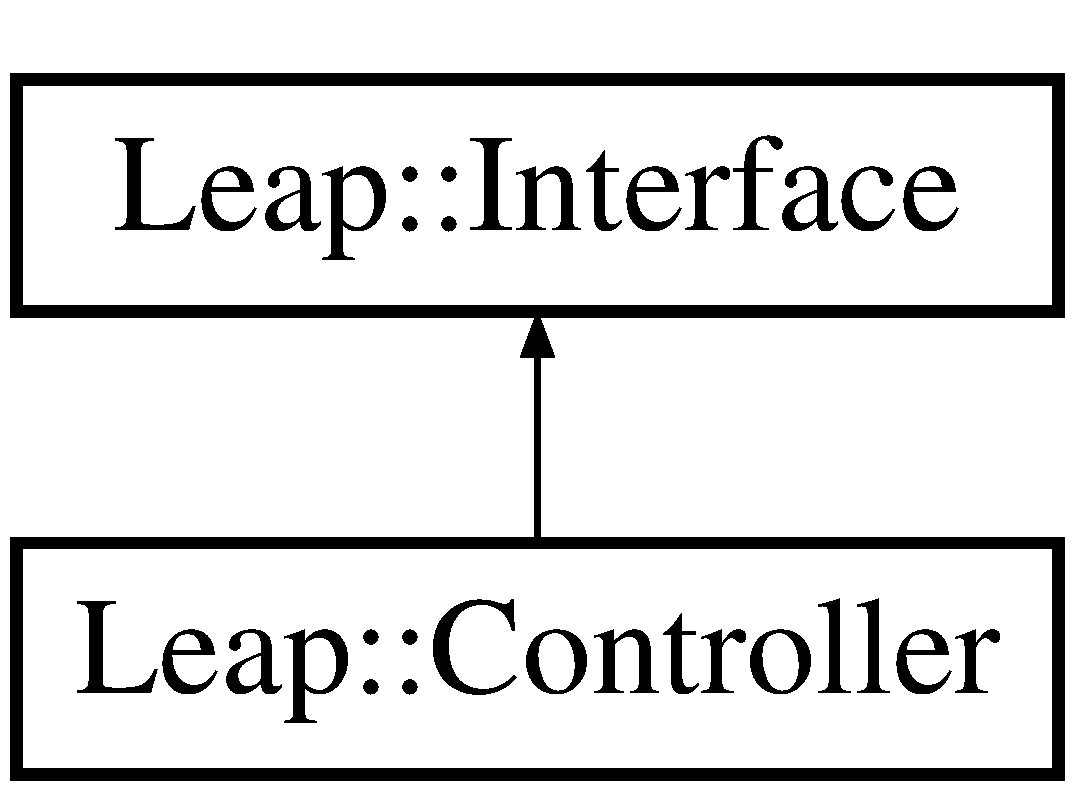
\includegraphics[height=2.000000cm]{class_leap_1_1_controller}
\end{center}
\end{figure}
\subsection*{Public Types}
\begin{DoxyCompactItemize}
\item 
enum \hyperlink{class_leap_1_1_controller_a0bdb49fa94aa2da8b098c1ac296528d6}{Policy\+Flag} \{ \hyperlink{class_leap_1_1_controller_a0bdb49fa94aa2da8b098c1ac296528d6a94886192cfa6f6f94cd2e20b68aeca97}{P\+O\+L\+I\+C\+Y\+\_\+\+D\+E\+F\+A\+U\+L\+T} = 0, 
\hyperlink{class_leap_1_1_controller_a0bdb49fa94aa2da8b098c1ac296528d6a1e34f1992444deee3b4c905d2a765329}{P\+O\+L\+I\+C\+Y\+\_\+\+B\+A\+C\+K\+G\+R\+O\+U\+N\+D\+\_\+\+F\+R\+A\+M\+E\+S} = (1 $<$$<$ 0)
 \}
\end{DoxyCompactItemize}
\subsection*{Public Member Functions}
\begin{DoxyCompactItemize}
\item 
\hypertarget{class_leap_1_1_controller_a356eee86e8cd232b3f6829986a64add5}{{\bfseries Controller} (Controller\+Implementation $\ast$)}\label{class_leap_1_1_controller_a356eee86e8cd232b3f6829986a64add5}

\item 
L\+E\+A\+P\+\_\+\+E\+X\+P\+O\+R\+T \hyperlink{class_leap_1_1_controller_af5867527cc80ad805597a285eaf3d406}{Controller} ()
\item 
L\+E\+A\+P\+\_\+\+E\+X\+P\+O\+R\+T \hyperlink{class_leap_1_1_controller_a046b09a621c480a46b3783551191abbb}{Controller} (\hyperlink{class_leap_1_1_listener}{Listener} \&listener)
\item 
L\+E\+A\+P\+\_\+\+E\+X\+P\+O\+R\+T bool \hyperlink{class_leap_1_1_controller_a1d7190d58adb6907d0e7c14d1ed595b4}{is\+Connected} () const 
\item 
L\+E\+A\+P\+\_\+\+E\+X\+P\+O\+R\+T bool \hyperlink{class_leap_1_1_controller_ab57ca1cb5b3278ff7016fa53028a1441}{has\+Focus} () const 
\item 
L\+E\+A\+P\+\_\+\+E\+X\+P\+O\+R\+T \hyperlink{class_leap_1_1_controller_a0bdb49fa94aa2da8b098c1ac296528d6}{Policy\+Flag} \hyperlink{class_leap_1_1_controller_af777725d8ab0793a03b5a9cee6e33480}{policy\+Flags} () const 
\item 
L\+E\+A\+P\+\_\+\+E\+X\+P\+O\+R\+T void \hyperlink{class_leap_1_1_controller_a9830f0a63b393ce83f3147101452d028}{set\+Policy\+Flags} (\hyperlink{class_leap_1_1_controller_a0bdb49fa94aa2da8b098c1ac296528d6}{Policy\+Flag} flags) const 
\item 
L\+E\+A\+P\+\_\+\+E\+X\+P\+O\+R\+T bool \hyperlink{class_leap_1_1_controller_a9b6318221593be63a0385748ca66974f}{add\+Listener} (\hyperlink{class_leap_1_1_listener}{Listener} \&listener)
\item 
L\+E\+A\+P\+\_\+\+E\+X\+P\+O\+R\+T bool \hyperlink{class_leap_1_1_controller_a1a48d46f317f0368cc8f7b0ebfd77728}{remove\+Listener} (\hyperlink{class_leap_1_1_listener}{Listener} \&listener)
\item 
L\+E\+A\+P\+\_\+\+E\+X\+P\+O\+R\+T \hyperlink{class_leap_1_1_frame}{Frame} \hyperlink{class_leap_1_1_controller_a5796b988806ea9fd94e2d987e0e24b32}{frame} (int history=0) const 
\item 
L\+E\+A\+P\+\_\+\+E\+X\+P\+O\+R\+T \hyperlink{class_leap_1_1_config}{Config} \hyperlink{class_leap_1_1_controller_abbb48ad47a8d0859a6a98f48c3d0a322}{config} () const 
\item 
L\+E\+A\+P\+\_\+\+E\+X\+P\+O\+R\+T \hyperlink{class_leap_1_1_device_list}{Device\+List} \hyperlink{class_leap_1_1_controller_a5dc199cb8f41cf07724c494107744251}{devices} () const 
\item 
L\+E\+A\+P\+\_\+\+E\+X\+P\+O\+R\+T \hyperlink{class_leap_1_1_screen_list}{Screen\+List} \hyperlink{class_leap_1_1_controller_ab6cf5b48ef434b3d58cf8962451f4df3}{located\+Screens} () const 
\item 
L\+E\+A\+P\+\_\+\+E\+X\+P\+O\+R\+T void \hyperlink{class_leap_1_1_controller_ad24410dee9de51b16ceb6b8c97fe5a36}{enable\+Gesture} (\hyperlink{class_leap_1_1_gesture_a6fa6dd4f28c502f0d55abc6b71c6f9b1}{Gesture\+::\+Type} type, bool enable=true) const 
\item 
L\+E\+A\+P\+\_\+\+E\+X\+P\+O\+R\+T bool \hyperlink{class_leap_1_1_controller_a8b3f3853d8cf1f805542006182c99729}{is\+Gesture\+Enabled} (\hyperlink{class_leap_1_1_gesture_a6fa6dd4f28c502f0d55abc6b71c6f9b1}{Gesture\+::\+Type} type) const 
\end{DoxyCompactItemize}
\subsection*{Additional Inherited Members}


\subsection{Detailed Description}
The \hyperlink{class_leap_1_1_controller}{Controller} class is your main interface to the Leap Motion \hyperlink{class_leap_1_1_controller}{Controller}.

Create an instance of this \hyperlink{class_leap_1_1_controller}{Controller} class to access frames of tracking data and configuration information. \hyperlink{class_leap_1_1_frame}{Frame} data can be polled at any time using the \hyperlink{class_leap_1_1_controller_a5796b988806ea9fd94e2d987e0e24b32}{Controller\+::frame()} function. Call \hyperlink{class_leap_1_1_controller_a5796b988806ea9fd94e2d987e0e24b32}{frame()} or frame(0) to get the most recent frame. Set the history parameter to a positive integer to access previous frames. A controller stores up to 60 frames in its frame history.

Polling is an appropriate strategy for applications which already have an intrinsic update loop, such as a game. You can also add an instance of a subclass of \hyperlink{class_leap_1_1_listener}{Leap\+::\+Listener} to the controller to handle events as they occur. The \hyperlink{class_leap_1_1_controller}{Controller} dispatches events to the listener upon initialization and exiting, on connection changes, when the application gains and loses the O\+S input focus, and when a new frame of tracking data is available. When these events occur, the controller object invokes the appropriate callback function defined in your subclass of \hyperlink{class_leap_1_1_listener}{Listener}.

To access frames of tracking data as they become available\+:


\begin{DoxyEnumerate}
\item Implement a subclass of the \hyperlink{class_leap_1_1_listener}{Listener} class and override the \hyperlink{class_leap_1_1_listener_ab600421108bbc952d8f0f144384ca30f}{Listener\+::on\+Frame()} function.
\item In your \hyperlink{class_leap_1_1_listener_ab600421108bbc952d8f0f144384ca30f}{Listener\+::on\+Frame()} function, call the \hyperlink{class_leap_1_1_controller_a5796b988806ea9fd94e2d987e0e24b32}{Controller\+::frame()} function to access the newest frame of tracking data.
\item To start receiving frames, create a \hyperlink{class_leap_1_1_controller}{Controller} object and add an instance of the \hyperlink{class_leap_1_1_listener}{Listener} subclass to the \hyperlink{class_leap_1_1_controller_a9b6318221593be63a0385748ca66974f}{Controller\+::add\+Listener()} function.
\end{DoxyEnumerate}

When an instance of a \hyperlink{class_leap_1_1_listener}{Listener} subclass is added to a \hyperlink{class_leap_1_1_controller}{Controller} object, it calls the \hyperlink{class_leap_1_1_listener_a180d621ad08afa5851d03d3546a82bbf}{Listener\+::on\+Init()} function when the listener is ready for use. When a connection is established between the controller and the Leap Motion software, the controller calls the \hyperlink{class_leap_1_1_listener_adfef79f9a03b342384aaa17f3a8ebf15}{Listener\+::on\+Connect()} function. At this point, your application will start receiving frames of data. The controller calls the \hyperlink{class_leap_1_1_listener_ab600421108bbc952d8f0f144384ca30f}{Listener\+::on\+Frame()} function each time a new frame is available. If the controller loses its connection with the Leap Motion software or device for any reason, it calls the \hyperlink{class_leap_1_1_listener_ac031e2d95b530097e2060518a9190f5e}{Listener\+::on\+Disconnect()} function. If the listener is removed from the controller or the controller is destroyed, it calls the \hyperlink{class_leap_1_1_listener_ac8f779a9208101f0084953560923f88c}{Listener\+::on\+Exit()} function. At that point, unless the listener is added to another controller again, it will no longer receive frames of tracking data.

The \hyperlink{class_leap_1_1_controller}{Controller} object is multithreaded and calls the \hyperlink{class_leap_1_1_listener}{Listener} functions on its own thread, not on an application thread. \begin{DoxySince}{Since}
1.\+0 
\end{DoxySince}


\subsection{Member Enumeration Documentation}
\hypertarget{class_leap_1_1_controller_a0bdb49fa94aa2da8b098c1ac296528d6}{\index{Leap\+::\+Controller@{Leap\+::\+Controller}!Policy\+Flag@{Policy\+Flag}}
\index{Policy\+Flag@{Policy\+Flag}!Leap\+::\+Controller@{Leap\+::\+Controller}}
\subsubsection[{Policy\+Flag}]{\setlength{\rightskip}{0pt plus 5cm}enum {\bf Leap\+::\+Controller\+::\+Policy\+Flag}}}\label{class_leap_1_1_controller_a0bdb49fa94aa2da8b098c1ac296528d6}
The supported controller policies.

Currently, the only supported policy is the background frames policy, which determines whether your application receives frames of tracking data when it is not the focused, foreground application. \begin{DoxySince}{Since}
1.\+0 
\end{DoxySince}
\begin{Desc}
\item[Enumerator]\par
\begin{description}
\index{P\+O\+L\+I\+C\+Y\+\_\+\+D\+E\+F\+A\+U\+L\+T@{P\+O\+L\+I\+C\+Y\+\_\+\+D\+E\+F\+A\+U\+L\+T}!Leap\+::\+Controller@{Leap\+::\+Controller}}\index{Leap\+::\+Controller@{Leap\+::\+Controller}!P\+O\+L\+I\+C\+Y\+\_\+\+D\+E\+F\+A\+U\+L\+T@{P\+O\+L\+I\+C\+Y\+\_\+\+D\+E\+F\+A\+U\+L\+T}}\item[{\em 
\hypertarget{class_leap_1_1_controller_a0bdb49fa94aa2da8b098c1ac296528d6a94886192cfa6f6f94cd2e20b68aeca97}{P\+O\+L\+I\+C\+Y\+\_\+\+D\+E\+F\+A\+U\+L\+T}\label{class_leap_1_1_controller_a0bdb49fa94aa2da8b098c1ac296528d6a94886192cfa6f6f94cd2e20b68aeca97}
}]The default policy. \begin{DoxySince}{Since}
1.\+0 
\end{DoxySince}
\index{P\+O\+L\+I\+C\+Y\+\_\+\+B\+A\+C\+K\+G\+R\+O\+U\+N\+D\+\_\+\+F\+R\+A\+M\+E\+S@{P\+O\+L\+I\+C\+Y\+\_\+\+B\+A\+C\+K\+G\+R\+O\+U\+N\+D\+\_\+\+F\+R\+A\+M\+E\+S}!Leap\+::\+Controller@{Leap\+::\+Controller}}\index{Leap\+::\+Controller@{Leap\+::\+Controller}!P\+O\+L\+I\+C\+Y\+\_\+\+B\+A\+C\+K\+G\+R\+O\+U\+N\+D\+\_\+\+F\+R\+A\+M\+E\+S@{P\+O\+L\+I\+C\+Y\+\_\+\+B\+A\+C\+K\+G\+R\+O\+U\+N\+D\+\_\+\+F\+R\+A\+M\+E\+S}}\item[{\em 
\hypertarget{class_leap_1_1_controller_a0bdb49fa94aa2da8b098c1ac296528d6a1e34f1992444deee3b4c905d2a765329}{P\+O\+L\+I\+C\+Y\+\_\+\+B\+A\+C\+K\+G\+R\+O\+U\+N\+D\+\_\+\+F\+R\+A\+M\+E\+S}\label{class_leap_1_1_controller_a0bdb49fa94aa2da8b098c1ac296528d6a1e34f1992444deee3b4c905d2a765329}
}]Receive background frames. \begin{DoxySince}{Since}
1.\+0 
\end{DoxySince}
\end{description}
\end{Desc}


\subsection{Constructor \& Destructor Documentation}
\hypertarget{class_leap_1_1_controller_af5867527cc80ad805597a285eaf3d406}{\index{Leap\+::\+Controller@{Leap\+::\+Controller}!Controller@{Controller}}
\index{Controller@{Controller}!Leap\+::\+Controller@{Leap\+::\+Controller}}
\subsubsection[{Controller}]{\setlength{\rightskip}{0pt plus 5cm}L\+E\+A\+P\+\_\+\+E\+X\+P\+O\+R\+T Leap\+::\+Controller\+::\+Controller (
\begin{DoxyParamCaption}
{}
\end{DoxyParamCaption}
)}}\label{class_leap_1_1_controller_af5867527cc80ad805597a285eaf3d406}
Constructs a \hyperlink{class_leap_1_1_controller}{Controller} object.

When creating a \hyperlink{class_leap_1_1_controller}{Controller} object, you may optionally pass in a reference to an instance of a subclass of \hyperlink{class_leap_1_1_listener}{Leap\+::\+Listener}. Alternatively, you may add a listener using the \hyperlink{class_leap_1_1_controller_a9b6318221593be63a0385748ca66974f}{Controller\+::add\+Listener()} function. \begin{DoxySince}{Since}
1.\+0 
\end{DoxySince}
\hypertarget{class_leap_1_1_controller_a046b09a621c480a46b3783551191abbb}{\index{Leap\+::\+Controller@{Leap\+::\+Controller}!Controller@{Controller}}
\index{Controller@{Controller}!Leap\+::\+Controller@{Leap\+::\+Controller}}
\subsubsection[{Controller}]{\setlength{\rightskip}{0pt plus 5cm}L\+E\+A\+P\+\_\+\+E\+X\+P\+O\+R\+T Leap\+::\+Controller\+::\+Controller (
\begin{DoxyParamCaption}
\item[{{\bf Listener} \&}]{listener}
\end{DoxyParamCaption}
)}}\label{class_leap_1_1_controller_a046b09a621c480a46b3783551191abbb}
Constructs a \hyperlink{class_leap_1_1_controller}{Controller} object.

When creating a \hyperlink{class_leap_1_1_controller}{Controller} object, you may optionally pass in a reference to an instance of a subclass of \hyperlink{class_leap_1_1_listener}{Leap\+::\+Listener}. Alternatively, you may add a listener using the \hyperlink{class_leap_1_1_controller_a9b6318221593be63a0385748ca66974f}{Controller\+::add\+Listener()} function.


\begin{DoxyParams}{Parameters}
{\em listener} & An instance of \hyperlink{class_leap_1_1_listener}{Leap\+::\+Listener} implementing the callback functions for the Leap Motion events you want to handle in your application. \\
\hline
\end{DoxyParams}
\begin{DoxySince}{Since}
1.\+0 
\end{DoxySince}


\subsection{Member Function Documentation}
\hypertarget{class_leap_1_1_controller_a9b6318221593be63a0385748ca66974f}{\index{Leap\+::\+Controller@{Leap\+::\+Controller}!add\+Listener@{add\+Listener}}
\index{add\+Listener@{add\+Listener}!Leap\+::\+Controller@{Leap\+::\+Controller}}
\subsubsection[{add\+Listener}]{\setlength{\rightskip}{0pt plus 5cm}L\+E\+A\+P\+\_\+\+E\+X\+P\+O\+R\+T bool Leap\+::\+Controller\+::add\+Listener (
\begin{DoxyParamCaption}
\item[{{\bf Listener} \&}]{listener}
\end{DoxyParamCaption}
)}}\label{class_leap_1_1_controller_a9b6318221593be63a0385748ca66974f}
Adds a listener to this \hyperlink{class_leap_1_1_controller}{Controller}.

The \hyperlink{class_leap_1_1_controller}{Controller} dispatches Leap Motion events to each associated listener. The order in which listener callback functions are invoked is arbitrary. If you pass a listener to the \hyperlink{class_leap_1_1_controller}{Controller}'s constructor function, it is automatically added to the list and can be removed with the \hyperlink{class_leap_1_1_controller_a1a48d46f317f0368cc8f7b0ebfd77728}{Controller\+::remove\+Listener()} function.


\begin{DoxyParams}{Parameters}
{\em listener} & A subclass of \hyperlink{class_leap_1_1_listener}{Leap\+::\+Listener} implementing the callback functions for the Leap Motion events you want to handle in your application. \\
\hline
\end{DoxyParams}
\begin{DoxyReturn}{Returns}
Whether or not the listener was successfully added to the list of listeners. 
\end{DoxyReturn}
\begin{DoxySince}{Since}
1.\+0 
\end{DoxySince}
\hypertarget{class_leap_1_1_controller_abbb48ad47a8d0859a6a98f48c3d0a322}{\index{Leap\+::\+Controller@{Leap\+::\+Controller}!config@{config}}
\index{config@{config}!Leap\+::\+Controller@{Leap\+::\+Controller}}
\subsubsection[{config}]{\setlength{\rightskip}{0pt plus 5cm}L\+E\+A\+P\+\_\+\+E\+X\+P\+O\+R\+T {\bf Config} Leap\+::\+Controller\+::config (
\begin{DoxyParamCaption}
{}
\end{DoxyParamCaption}
) const}}\label{class_leap_1_1_controller_abbb48ad47a8d0859a6a98f48c3d0a322}
Returns a \hyperlink{class_leap_1_1_config}{Config} object, which you can use to query the Leap Motion system for configuration information. \begin{DoxySince}{Since}
1.\+0 
\end{DoxySince}
\hypertarget{class_leap_1_1_controller_a5dc199cb8f41cf07724c494107744251}{\index{Leap\+::\+Controller@{Leap\+::\+Controller}!devices@{devices}}
\index{devices@{devices}!Leap\+::\+Controller@{Leap\+::\+Controller}}
\subsubsection[{devices}]{\setlength{\rightskip}{0pt plus 5cm}L\+E\+A\+P\+\_\+\+E\+X\+P\+O\+R\+T {\bf Device\+List} Leap\+::\+Controller\+::devices (
\begin{DoxyParamCaption}
{}
\end{DoxyParamCaption}
) const}}\label{class_leap_1_1_controller_a5dc199cb8f41cf07724c494107744251}
The list of currently attached and recognized Leap Motion controller devices.

The \hyperlink{class_leap_1_1_device}{Device} objects in the list describe information such as the range and tracking volume.

Currently, the Leap Motion \hyperlink{class_leap_1_1_controller}{Controller} only recognizes a single device at a time. \begin{DoxySince}{Since}
1.\+0 
\end{DoxySince}
\hypertarget{class_leap_1_1_controller_ad24410dee9de51b16ceb6b8c97fe5a36}{\index{Leap\+::\+Controller@{Leap\+::\+Controller}!enable\+Gesture@{enable\+Gesture}}
\index{enable\+Gesture@{enable\+Gesture}!Leap\+::\+Controller@{Leap\+::\+Controller}}
\subsubsection[{enable\+Gesture}]{\setlength{\rightskip}{0pt plus 5cm}L\+E\+A\+P\+\_\+\+E\+X\+P\+O\+R\+T void Leap\+::\+Controller\+::enable\+Gesture (
\begin{DoxyParamCaption}
\item[{{\bf Gesture\+::\+Type}}]{type, }
\item[{bool}]{enable = {\ttfamily true}}
\end{DoxyParamCaption}
) const}}\label{class_leap_1_1_controller_ad24410dee9de51b16ceb6b8c97fe5a36}
Enables or disables reporting of a specified gesture type.

By default, all gesture types are disabled. When disabled, gestures of the disabled type are never reported and will not appear in the frame gesture list.

As a performance optimization, only enable recognition for the types of movements that you use in your application.


\begin{DoxyParams}{Parameters}
{\em type} & The type of gesture to enable or disable. Must be a member of the \hyperlink{class_leap_1_1_gesture_a6fa6dd4f28c502f0d55abc6b71c6f9b1}{Gesture\+::\+Type} enumeration. \\
\hline
{\em enable} & True, to enable the specified gesture type; False, to disable. \\
\hline
\end{DoxyParams}
\begin{DoxySeeAlso}{See also}
\hyperlink{class_leap_1_1_controller_a8b3f3853d8cf1f805542006182c99729}{Controller\+::is\+Gesture\+Enabled()} 
\end{DoxySeeAlso}
\begin{DoxySince}{Since}
1.\+0 
\end{DoxySince}
\hypertarget{class_leap_1_1_controller_a5796b988806ea9fd94e2d987e0e24b32}{\index{Leap\+::\+Controller@{Leap\+::\+Controller}!frame@{frame}}
\index{frame@{frame}!Leap\+::\+Controller@{Leap\+::\+Controller}}
\subsubsection[{frame}]{\setlength{\rightskip}{0pt plus 5cm}L\+E\+A\+P\+\_\+\+E\+X\+P\+O\+R\+T {\bf Frame} Leap\+::\+Controller\+::frame (
\begin{DoxyParamCaption}
\item[{int}]{history = {\ttfamily 0}}
\end{DoxyParamCaption}
) const}}\label{class_leap_1_1_controller_a5796b988806ea9fd94e2d987e0e24b32}
Returns a frame of tracking data from the Leap Motion software. Use the optional history parameter to specify which frame to retrieve. Call \hyperlink{class_leap_1_1_controller_a5796b988806ea9fd94e2d987e0e24b32}{frame()} or frame(0) to access the most recent frame; call frame(1) to access the previous frame, and so on. If you use a history value greater than the number of stored frames, then the controller returns an invalid frame.


\begin{DoxyParams}{Parameters}
{\em history} & The age of the frame to return, counting backwards from the most recent frame (0) into the past and up to the maximum age (59). \\
\hline
\end{DoxyParams}
\begin{DoxyReturn}{Returns}
The specified frame; or, if no history parameter is specified, the newest frame. If a frame is not available at the specified history position, an invalid \hyperlink{class_leap_1_1_frame}{Frame} is returned. 
\end{DoxyReturn}
\begin{DoxySince}{Since}
1.\+0 
\end{DoxySince}
\hypertarget{class_leap_1_1_controller_ab57ca1cb5b3278ff7016fa53028a1441}{\index{Leap\+::\+Controller@{Leap\+::\+Controller}!has\+Focus@{has\+Focus}}
\index{has\+Focus@{has\+Focus}!Leap\+::\+Controller@{Leap\+::\+Controller}}
\subsubsection[{has\+Focus}]{\setlength{\rightskip}{0pt plus 5cm}L\+E\+A\+P\+\_\+\+E\+X\+P\+O\+R\+T bool Leap\+::\+Controller\+::has\+Focus (
\begin{DoxyParamCaption}
{}
\end{DoxyParamCaption}
) const}}\label{class_leap_1_1_controller_ab57ca1cb5b3278ff7016fa53028a1441}
Reports whether this application is the focused, foreground application.

By default, your application only receives tracking information from the Leap Motion controller when it has the operating system input focus. To receive tracking data when your application is in the background, the background frames policy flag must be set.

\begin{DoxyReturn}{Returns}
True, if application has focus; false otherwise.
\end{DoxyReturn}
\begin{DoxySeeAlso}{See also}
\hyperlink{class_leap_1_1_controller_a9830f0a63b393ce83f3147101452d028}{Controller\+::set\+Policy\+Flags()} 
\end{DoxySeeAlso}
\begin{DoxySince}{Since}
1.\+0 
\end{DoxySince}
\hypertarget{class_leap_1_1_controller_a1d7190d58adb6907d0e7c14d1ed595b4}{\index{Leap\+::\+Controller@{Leap\+::\+Controller}!is\+Connected@{is\+Connected}}
\index{is\+Connected@{is\+Connected}!Leap\+::\+Controller@{Leap\+::\+Controller}}
\subsubsection[{is\+Connected}]{\setlength{\rightskip}{0pt plus 5cm}L\+E\+A\+P\+\_\+\+E\+X\+P\+O\+R\+T bool Leap\+::\+Controller\+::is\+Connected (
\begin{DoxyParamCaption}
{}
\end{DoxyParamCaption}
) const}}\label{class_leap_1_1_controller_a1d7190d58adb6907d0e7c14d1ed595b4}
Reports whether this \hyperlink{class_leap_1_1_controller}{Controller} is connected to the Leap Motion \hyperlink{class_leap_1_1_controller}{Controller}.

When you first create a \hyperlink{class_leap_1_1_controller}{Controller} object, \hyperlink{class_leap_1_1_controller_a1d7190d58adb6907d0e7c14d1ed595b4}{is\+Connected()} returns false. After the controller finishes initializing and connects to the Leap Motion software, \hyperlink{class_leap_1_1_controller_a1d7190d58adb6907d0e7c14d1ed595b4}{is\+Connected()} will return true.

You can either handle the on\+Connect event using a \hyperlink{class_leap_1_1_listener}{Listener} instance or poll the \hyperlink{class_leap_1_1_controller_a1d7190d58adb6907d0e7c14d1ed595b4}{is\+Connected()} function if you need to wait for your application to be connected to the Leap Motion software before performing some other operation.

\begin{DoxyReturn}{Returns}
True, if connected; false otherwise. 
\end{DoxyReturn}
\begin{DoxySince}{Since}
1.\+0 
\end{DoxySince}
\hypertarget{class_leap_1_1_controller_a8b3f3853d8cf1f805542006182c99729}{\index{Leap\+::\+Controller@{Leap\+::\+Controller}!is\+Gesture\+Enabled@{is\+Gesture\+Enabled}}
\index{is\+Gesture\+Enabled@{is\+Gesture\+Enabled}!Leap\+::\+Controller@{Leap\+::\+Controller}}
\subsubsection[{is\+Gesture\+Enabled}]{\setlength{\rightskip}{0pt plus 5cm}L\+E\+A\+P\+\_\+\+E\+X\+P\+O\+R\+T bool Leap\+::\+Controller\+::is\+Gesture\+Enabled (
\begin{DoxyParamCaption}
\item[{{\bf Gesture\+::\+Type}}]{type}
\end{DoxyParamCaption}
) const}}\label{class_leap_1_1_controller_a8b3f3853d8cf1f805542006182c99729}
Reports whether the specified gesture type is enabled.

\begin{DoxyReturn}{Returns}
True, if the specified type is enabled; false, otherwise. 
\end{DoxyReturn}
\begin{DoxySeeAlso}{See also}
\hyperlink{class_leap_1_1_controller_ad24410dee9de51b16ceb6b8c97fe5a36}{Controller\+::enable\+Gesture()} 
\end{DoxySeeAlso}
\begin{DoxySince}{Since}
1.\+0 
\end{DoxySince}
\hypertarget{class_leap_1_1_controller_ab6cf5b48ef434b3d58cf8962451f4df3}{\index{Leap\+::\+Controller@{Leap\+::\+Controller}!located\+Screens@{located\+Screens}}
\index{located\+Screens@{located\+Screens}!Leap\+::\+Controller@{Leap\+::\+Controller}}
\subsubsection[{located\+Screens}]{\setlength{\rightskip}{0pt plus 5cm}L\+E\+A\+P\+\_\+\+E\+X\+P\+O\+R\+T {\bf Screen\+List} Leap\+::\+Controller\+::located\+Screens (
\begin{DoxyParamCaption}
{}
\end{DoxyParamCaption}
) const}}\label{class_leap_1_1_controller_ab6cf5b48ef434b3d58cf8962451f4df3}
The list of screens whose positions have been identified by using the Leap Motion \hyperlink{class_leap_1_1_screen}{Screen} Locator.

The list always contains at least one entry representing the default screen. If the user has not registered the location of this default screen, then the coordinates, directions, and other values reported by the functions in its \hyperlink{class_leap_1_1_screen}{Screen} object will not be accurate. Other monitor screens only appear in the list if their positions have been registered using the Leap Motion \hyperlink{class_leap_1_1_screen}{Screen} Locator.

A \hyperlink{class_leap_1_1_screen}{Screen} object represents the position and orientation of a display monitor screen within the Leap Motion coordinate system. For example, if the screen location is known, you can get Leap Motion coordinates for the bottom-\/left corner of the screen. Registering the screen location also allows the Leap Motion software to calculate the point on the screen at which a finger or tool is pointing.

A user can run the \hyperlink{class_leap_1_1_screen}{Screen} Locator tool from the Leap Motion Settings dialog. Avoid assuming that a screen location is known or that an existing position is still correct. The registered position is only valid as long as the relative position of the Leap Motion \hyperlink{class_leap_1_1_controller}{Controller} and the monitor screen remain constant.


\begin{DoxyCodeInclude}
\end{DoxyCodeInclude}


\begin{DoxyReturn}{Returns}
\hyperlink{class_leap_1_1_screen_list}{Screen\+List} A list containing the screens whose positions have been registered by the user using the \hyperlink{class_leap_1_1_screen}{Screen} Locator tool. The list always contains at least one entry representing the default monitor. If the user has not run the \hyperlink{class_leap_1_1_screen}{Screen} Locator or has moved the Leap Motion device or screen since running it, the \hyperlink{class_leap_1_1_screen}{Screen} object for this entry only contains default values. 
\end{DoxyReturn}
\begin{DoxySince}{Since}
1.\+0 
\end{DoxySince}
\hypertarget{class_leap_1_1_controller_af777725d8ab0793a03b5a9cee6e33480}{\index{Leap\+::\+Controller@{Leap\+::\+Controller}!policy\+Flags@{policy\+Flags}}
\index{policy\+Flags@{policy\+Flags}!Leap\+::\+Controller@{Leap\+::\+Controller}}
\subsubsection[{policy\+Flags}]{\setlength{\rightskip}{0pt plus 5cm}L\+E\+A\+P\+\_\+\+E\+X\+P\+O\+R\+T {\bf Policy\+Flag} Leap\+::\+Controller\+::policy\+Flags (
\begin{DoxyParamCaption}
{}
\end{DoxyParamCaption}
) const}}\label{class_leap_1_1_controller_af777725d8ab0793a03b5a9cee6e33480}
Gets the active policy settings.

Use this function to determine the current policy state. Keep in mind that setting a policy flag is asynchronous, so changes are not effective immediately after calling set\+Policy\+Flag(). In addition, a policy request can be declined by the user. You should always set the policy flags required by your application at startup and check that the policy change request was successful after an appropriate interval.

If the controller object is not connected to the Leap Motion software, then the default policy state is returned.

\begin{DoxyReturn}{Returns}
The current policy flags. 
\end{DoxyReturn}
\begin{DoxySince}{Since}
1.\+0 
\end{DoxySince}
\hypertarget{class_leap_1_1_controller_a1a48d46f317f0368cc8f7b0ebfd77728}{\index{Leap\+::\+Controller@{Leap\+::\+Controller}!remove\+Listener@{remove\+Listener}}
\index{remove\+Listener@{remove\+Listener}!Leap\+::\+Controller@{Leap\+::\+Controller}}
\subsubsection[{remove\+Listener}]{\setlength{\rightskip}{0pt plus 5cm}L\+E\+A\+P\+\_\+\+E\+X\+P\+O\+R\+T bool Leap\+::\+Controller\+::remove\+Listener (
\begin{DoxyParamCaption}
\item[{{\bf Listener} \&}]{listener}
\end{DoxyParamCaption}
)}}\label{class_leap_1_1_controller_a1a48d46f317f0368cc8f7b0ebfd77728}
Remove a listener from the list of listeners that will receive Leap Motion events. A listener must be removed if its lifetime is shorter than the controller to which it is listening.


\begin{DoxyParams}{Parameters}
{\em listener} & The listener to remove. \\
\hline
\end{DoxyParams}
\begin{DoxyReturn}{Returns}
Whether or not the listener was successfully removed from the list of listeners. 
\end{DoxyReturn}
\begin{DoxySince}{Since}
1.\+0 
\end{DoxySince}
\hypertarget{class_leap_1_1_controller_a9830f0a63b393ce83f3147101452d028}{\index{Leap\+::\+Controller@{Leap\+::\+Controller}!set\+Policy\+Flags@{set\+Policy\+Flags}}
\index{set\+Policy\+Flags@{set\+Policy\+Flags}!Leap\+::\+Controller@{Leap\+::\+Controller}}
\subsubsection[{set\+Policy\+Flags}]{\setlength{\rightskip}{0pt plus 5cm}L\+E\+A\+P\+\_\+\+E\+X\+P\+O\+R\+T void Leap\+::\+Controller\+::set\+Policy\+Flags (
\begin{DoxyParamCaption}
\item[{{\bf Policy\+Flag}}]{flags}
\end{DoxyParamCaption}
) const}}\label{class_leap_1_1_controller_a9830f0a63b393ce83f3147101452d028}
Requests a change in policy.

A request to change a policy is subject to user approval and a policy can be changed by the user at any time (using the Leap Motion settings dialog). The desired policy flags must be set every time an application runs.

Policy changes are completed asynchronously and, because they are subject to user approval, may not complete successfully. Call \hyperlink{class_leap_1_1_controller_af777725d8ab0793a03b5a9cee6e33480}{Controller\+::policy\+Flags()} after a suitable interval to test whether the change was accepted.

Currently, the background frames policy is the only policy supported. The background frames policy determines whether an application receives frames of tracking data while in the background. By default, the Leap Motion software only sends tracking data to the foreground application. Only applications that need this ability should request the background frames policy.

At this time, you can use the Leap Motion Settings dialog to globally enable or disable the background frames policy. However, each application that needs tracking data while in the background must also set the policy flag using this function.

This function can be called before the \hyperlink{class_leap_1_1_controller}{Controller} object is connected, but the request will be sent to the Leap Motion software after the \hyperlink{class_leap_1_1_controller}{Controller} connects.


\begin{DoxyParams}{Parameters}
{\em flags} & A Policy\+Flag value indicating the policies to request. \\
\hline
\end{DoxyParams}
\begin{DoxySince}{Since}
1.\+0 
\end{DoxySince}


The documentation for this class was generated from the following file\+:\begin{DoxyCompactItemize}
\item 
Interface\+Managers/Leap.\+h\end{DoxyCompactItemize}

\hypertarget{class_leap_1_1_device}{\section{Leap\+:\+:Device Class Reference}
\label{class_leap_1_1_device}\index{Leap\+::\+Device@{Leap\+::\+Device}}
}


{\ttfamily \#include $<$Leap.\+h$>$}

Inheritance diagram for Leap\+:\+:Device\+:\begin{figure}[H]
\begin{center}
\leavevmode
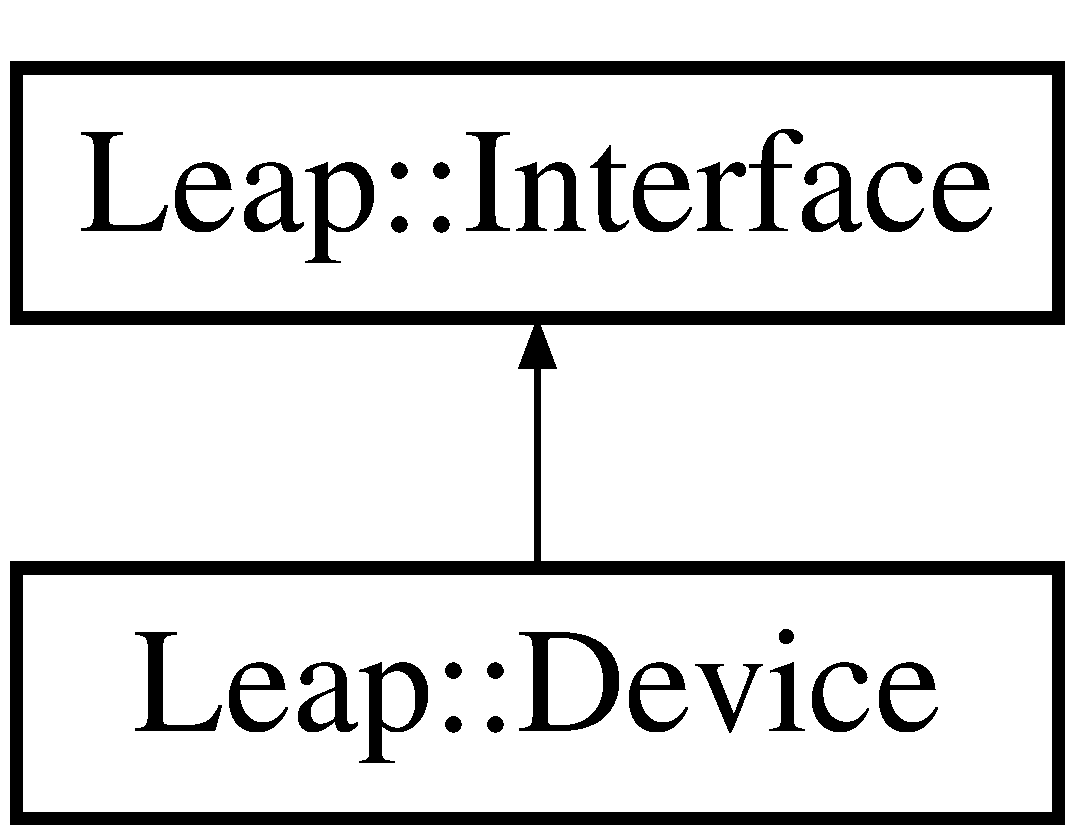
\includegraphics[height=2.000000cm]{class_leap_1_1_device}
\end{center}
\end{figure}
\subsection*{Public Member Functions}
\begin{DoxyCompactItemize}
\item 
\hypertarget{class_leap_1_1_device_a7ec1c5a141f6b5de72846944fad60066}{{\bfseries Device} (Device\+Implementation $\ast$)}\label{class_leap_1_1_device_a7ec1c5a141f6b5de72846944fad60066}

\item 
L\+E\+A\+P\+\_\+\+E\+X\+P\+O\+R\+T \hyperlink{class_leap_1_1_device_ab14c21cd02a6773fa699980cb58032e2}{Device} ()
\item 
L\+E\+A\+P\+\_\+\+E\+X\+P\+O\+R\+T float \hyperlink{class_leap_1_1_device_a50aebd24cb616913c93776776bb34599}{horizontal\+View\+Angle} () const 
\item 
L\+E\+A\+P\+\_\+\+E\+X\+P\+O\+R\+T float \hyperlink{class_leap_1_1_device_a7d897c54bc650faf204fd2d2a1e8dfc5}{vertical\+View\+Angle} () const 
\item 
L\+E\+A\+P\+\_\+\+E\+X\+P\+O\+R\+T float \hyperlink{class_leap_1_1_device_a110a7177c29ccea229e554c488596a4d}{range} () const 
\item 
L\+E\+A\+P\+\_\+\+E\+X\+P\+O\+R\+T float \hyperlink{class_leap_1_1_device_a564bfe97e86eb5440093098d383cc5b2}{distance\+To\+Boundary} (const \hyperlink{struct_leap_1_1_vector}{Vector} \&position) const 
\item 
L\+E\+A\+P\+\_\+\+E\+X\+P\+O\+R\+T bool \hyperlink{class_leap_1_1_device_a26b77ec606519bb486e79d187bc8fae0}{is\+Valid} () const 
\item 
L\+E\+A\+P\+\_\+\+E\+X\+P\+O\+R\+T bool \hyperlink{class_leap_1_1_device_a20c6e9191d90de43b66def39d187e74e}{operator==} (const \hyperlink{class_leap_1_1_device}{Device} \&) const 
\item 
L\+E\+A\+P\+\_\+\+E\+X\+P\+O\+R\+T bool \hyperlink{class_leap_1_1_device_aa80064c6642078ab84652e4e984ec4fc}{operator!=} (const \hyperlink{class_leap_1_1_device}{Device} \&) const 
\item 
L\+E\+A\+P\+\_\+\+E\+X\+P\+O\+R\+T std\+::string \hyperlink{class_leap_1_1_device_ac498246027e86561a541178cc622761c}{to\+String} () const 
\end{DoxyCompactItemize}
\subsection*{Static Public Member Functions}
\begin{DoxyCompactItemize}
\item 
static L\+E\+A\+P\+\_\+\+E\+X\+P\+O\+R\+T const \hyperlink{class_leap_1_1_device}{Device} \& \hyperlink{class_leap_1_1_device_a4a87905142db30a40b47b428db495db6}{invalid} ()
\end{DoxyCompactItemize}
\subsection*{Friends}
\begin{DoxyCompactItemize}
\item 
L\+E\+A\+P\+\_\+\+E\+X\+P\+O\+R\+T friend std\+::ostream \& \hyperlink{class_leap_1_1_device_a5296f0c6d7b410e2ffc23c6e74a507ec}{operator$<$$<$} (std\+::ostream \&, const \hyperlink{class_leap_1_1_device}{Device} \&)
\end{DoxyCompactItemize}
\subsection*{Additional Inherited Members}


\subsection{Detailed Description}
The \hyperlink{class_leap_1_1_device}{Device} class represents a physically connected device.

The \hyperlink{class_leap_1_1_device}{Device} class contains information related to a particular connected device such as field of view, device id, and calibrated positions.

Note that \hyperlink{class_leap_1_1_device}{Device} objects can be invalid, which means that they do not contain valid device information and do not correspond to a physical device. Test for validity with the \hyperlink{class_leap_1_1_device_a26b77ec606519bb486e79d187bc8fae0}{Device\+::is\+Valid()} function. \begin{DoxySince}{Since}
1.\+0 
\end{DoxySince}


\subsection{Constructor \& Destructor Documentation}
\hypertarget{class_leap_1_1_device_ab14c21cd02a6773fa699980cb58032e2}{\index{Leap\+::\+Device@{Leap\+::\+Device}!Device@{Device}}
\index{Device@{Device}!Leap\+::\+Device@{Leap\+::\+Device}}
\subsubsection[{Device}]{\setlength{\rightskip}{0pt plus 5cm}L\+E\+A\+P\+\_\+\+E\+X\+P\+O\+R\+T Leap\+::\+Device\+::\+Device (
\begin{DoxyParamCaption}
{}
\end{DoxyParamCaption}
)}}\label{class_leap_1_1_device_ab14c21cd02a6773fa699980cb58032e2}
Constructs a \hyperlink{class_leap_1_1_device}{Device} object.

An uninitialized device is considered invalid. Get valid \hyperlink{class_leap_1_1_device}{Device} objects from a \hyperlink{class_leap_1_1_device_list}{Device\+List} object obtained using the \hyperlink{class_leap_1_1_controller_a5dc199cb8f41cf07724c494107744251}{Controller\+::devices()} method. \begin{DoxySince}{Since}
1.\+0 
\end{DoxySince}


\subsection{Member Function Documentation}
\hypertarget{class_leap_1_1_device_a564bfe97e86eb5440093098d383cc5b2}{\index{Leap\+::\+Device@{Leap\+::\+Device}!distance\+To\+Boundary@{distance\+To\+Boundary}}
\index{distance\+To\+Boundary@{distance\+To\+Boundary}!Leap\+::\+Device@{Leap\+::\+Device}}
\subsubsection[{distance\+To\+Boundary}]{\setlength{\rightskip}{0pt plus 5cm}L\+E\+A\+P\+\_\+\+E\+X\+P\+O\+R\+T float Leap\+::\+Device\+::distance\+To\+Boundary (
\begin{DoxyParamCaption}
\item[{const {\bf Vector} \&}]{position}
\end{DoxyParamCaption}
) const}}\label{class_leap_1_1_device_a564bfe97e86eb5440093098d383cc5b2}
The distance to the nearest edge of the Leap Motion controller's view volume.

The view volume is an axis-\/aligned, inverted pyramid centered on the device origin and extending upward to the range limit. The walls of the pyramid are described by the horizontal\+View\+Angle and vertical\+View\+Angle and the roof by the range. This function estimates the distance between the specified input position and the nearest wall or roof of the view volume.


\begin{DoxyParams}{Parameters}
{\em position} & The point to use for the distance calculation. \\
\hline
\end{DoxyParams}
\begin{DoxyReturn}{Returns}
The distance in millimeters from the input position to the nearest boundary. 
\end{DoxyReturn}
\begin{DoxySince}{Since}
1.\+0 
\end{DoxySince}
\hypertarget{class_leap_1_1_device_a50aebd24cb616913c93776776bb34599}{\index{Leap\+::\+Device@{Leap\+::\+Device}!horizontal\+View\+Angle@{horizontal\+View\+Angle}}
\index{horizontal\+View\+Angle@{horizontal\+View\+Angle}!Leap\+::\+Device@{Leap\+::\+Device}}
\subsubsection[{horizontal\+View\+Angle}]{\setlength{\rightskip}{0pt plus 5cm}L\+E\+A\+P\+\_\+\+E\+X\+P\+O\+R\+T float Leap\+::\+Device\+::horizontal\+View\+Angle (
\begin{DoxyParamCaption}
{}
\end{DoxyParamCaption}
) const}}\label{class_leap_1_1_device_a50aebd24cb616913c93776776bb34599}
The angle of view along the x axis of this device.



The Leap Motion controller scans a region in the shape of an inverted pyramid centered at the device's center and extending upwards. The horizontal\+View\+Angle reports the view angle along the long dimension of the device.

\begin{DoxyReturn}{Returns}
The horizontal angle of view in radians. 
\end{DoxyReturn}
\begin{DoxySince}{Since}
1.\+0 
\end{DoxySince}
\hypertarget{class_leap_1_1_device_a4a87905142db30a40b47b428db495db6}{\index{Leap\+::\+Device@{Leap\+::\+Device}!invalid@{invalid}}
\index{invalid@{invalid}!Leap\+::\+Device@{Leap\+::\+Device}}
\subsubsection[{invalid}]{\setlength{\rightskip}{0pt plus 5cm}static L\+E\+A\+P\+\_\+\+E\+X\+P\+O\+R\+T const {\bf Device}\& Leap\+::\+Device\+::invalid (
\begin{DoxyParamCaption}
{}
\end{DoxyParamCaption}
)\hspace{0.3cm}{\ttfamily [static]}}}\label{class_leap_1_1_device_a4a87905142db30a40b47b428db495db6}
Returns an invalid \hyperlink{class_leap_1_1_device}{Device} object.

You can use the instance returned by this function in comparisons testing whether a given \hyperlink{class_leap_1_1_device}{Device} instance is valid or invalid. (You can also use the \hyperlink{class_leap_1_1_device_a26b77ec606519bb486e79d187bc8fae0}{Device\+::is\+Valid()} function.)

\begin{DoxyReturn}{Returns}
The invalid \hyperlink{class_leap_1_1_device}{Device} instance. 
\end{DoxyReturn}
\begin{DoxySince}{Since}
1.\+0 
\end{DoxySince}
\hypertarget{class_leap_1_1_device_a26b77ec606519bb486e79d187bc8fae0}{\index{Leap\+::\+Device@{Leap\+::\+Device}!is\+Valid@{is\+Valid}}
\index{is\+Valid@{is\+Valid}!Leap\+::\+Device@{Leap\+::\+Device}}
\subsubsection[{is\+Valid}]{\setlength{\rightskip}{0pt plus 5cm}L\+E\+A\+P\+\_\+\+E\+X\+P\+O\+R\+T bool Leap\+::\+Device\+::is\+Valid (
\begin{DoxyParamCaption}
{}
\end{DoxyParamCaption}
) const}}\label{class_leap_1_1_device_a26b77ec606519bb486e79d187bc8fae0}
Reports whether this is a valid \hyperlink{class_leap_1_1_device}{Device} object.

\begin{DoxyReturn}{Returns}
True, if this \hyperlink{class_leap_1_1_device}{Device} object contains valid data. 
\end{DoxyReturn}
\begin{DoxySince}{Since}
1.\+0 
\end{DoxySince}
\hypertarget{class_leap_1_1_device_aa80064c6642078ab84652e4e984ec4fc}{\index{Leap\+::\+Device@{Leap\+::\+Device}!operator"!=@{operator"!=}}
\index{operator"!=@{operator"!=}!Leap\+::\+Device@{Leap\+::\+Device}}
\subsubsection[{operator"!=}]{\setlength{\rightskip}{0pt plus 5cm}L\+E\+A\+P\+\_\+\+E\+X\+P\+O\+R\+T bool Leap\+::\+Device\+::operator!= (
\begin{DoxyParamCaption}
\item[{const {\bf Device} \&}]{}
\end{DoxyParamCaption}
) const}}\label{class_leap_1_1_device_aa80064c6642078ab84652e4e984ec4fc}
Compare \hyperlink{class_leap_1_1_device}{Device} object inequality.

Two \hyperlink{class_leap_1_1_device}{Device} objects are equal if and only if both \hyperlink{class_leap_1_1_device}{Device} objects represent the exact same \hyperlink{class_leap_1_1_device}{Device} and both Devices are valid. \begin{DoxySince}{Since}
1.\+0 
\end{DoxySince}
\hypertarget{class_leap_1_1_device_a20c6e9191d90de43b66def39d187e74e}{\index{Leap\+::\+Device@{Leap\+::\+Device}!operator==@{operator==}}
\index{operator==@{operator==}!Leap\+::\+Device@{Leap\+::\+Device}}
\subsubsection[{operator==}]{\setlength{\rightskip}{0pt plus 5cm}L\+E\+A\+P\+\_\+\+E\+X\+P\+O\+R\+T bool Leap\+::\+Device\+::operator== (
\begin{DoxyParamCaption}
\item[{const {\bf Device} \&}]{}
\end{DoxyParamCaption}
) const}}\label{class_leap_1_1_device_a20c6e9191d90de43b66def39d187e74e}
Compare \hyperlink{class_leap_1_1_device}{Device} object equality.

Two \hyperlink{class_leap_1_1_device}{Device} objects are equal if and only if both \hyperlink{class_leap_1_1_device}{Device} objects represent the exact same \hyperlink{class_leap_1_1_device}{Device} and both Devices are valid. \begin{DoxySince}{Since}
1.\+0 
\end{DoxySince}
\hypertarget{class_leap_1_1_device_a110a7177c29ccea229e554c488596a4d}{\index{Leap\+::\+Device@{Leap\+::\+Device}!range@{range}}
\index{range@{range}!Leap\+::\+Device@{Leap\+::\+Device}}
\subsubsection[{range}]{\setlength{\rightskip}{0pt plus 5cm}L\+E\+A\+P\+\_\+\+E\+X\+P\+O\+R\+T float Leap\+::\+Device\+::range (
\begin{DoxyParamCaption}
{}
\end{DoxyParamCaption}
) const}}\label{class_leap_1_1_device_a110a7177c29ccea229e554c488596a4d}
The maximum reliable tracking range.

The range reports the maximum recommended distance from the device center for which tracking is expected to be reliable. This distance is not a hard limit. Tracking may be still be functional above this distance or begin to degrade slightly before this distance depending on calibration and extreme environmental conditions.

\begin{DoxyReturn}{Returns}
The recommended maximum range of the device in mm. 
\end{DoxyReturn}
\begin{DoxySince}{Since}
1.\+0 
\end{DoxySince}
\hypertarget{class_leap_1_1_device_ac498246027e86561a541178cc622761c}{\index{Leap\+::\+Device@{Leap\+::\+Device}!to\+String@{to\+String}}
\index{to\+String@{to\+String}!Leap\+::\+Device@{Leap\+::\+Device}}
\subsubsection[{to\+String}]{\setlength{\rightskip}{0pt plus 5cm}L\+E\+A\+P\+\_\+\+E\+X\+P\+O\+R\+T std\+::string Leap\+::\+Device\+::to\+String (
\begin{DoxyParamCaption}
{}
\end{DoxyParamCaption}
) const}}\label{class_leap_1_1_device_ac498246027e86561a541178cc622761c}
A string containing a brief, human readable description of the \hyperlink{class_leap_1_1_device}{Device} object.

\begin{DoxyReturn}{Returns}
A description of the \hyperlink{class_leap_1_1_device}{Device} as a string. 
\end{DoxyReturn}
\begin{DoxySince}{Since}
1.\+0 
\end{DoxySince}
\hypertarget{class_leap_1_1_device_a7d897c54bc650faf204fd2d2a1e8dfc5}{\index{Leap\+::\+Device@{Leap\+::\+Device}!vertical\+View\+Angle@{vertical\+View\+Angle}}
\index{vertical\+View\+Angle@{vertical\+View\+Angle}!Leap\+::\+Device@{Leap\+::\+Device}}
\subsubsection[{vertical\+View\+Angle}]{\setlength{\rightskip}{0pt plus 5cm}L\+E\+A\+P\+\_\+\+E\+X\+P\+O\+R\+T float Leap\+::\+Device\+::vertical\+View\+Angle (
\begin{DoxyParamCaption}
{}
\end{DoxyParamCaption}
) const}}\label{class_leap_1_1_device_a7d897c54bc650faf204fd2d2a1e8dfc5}
The angle of view along the z axis of this device.



The Leap Motion controller scans a region in the shape of an inverted pyramid centered at the device's center and extending upwards. The vertical\+View\+Angle reports the view angle along the short dimension of the device.

\begin{DoxyReturn}{Returns}
The vertical angle of view in radians. 
\end{DoxyReturn}
\begin{DoxySince}{Since}
1.\+0 
\end{DoxySince}


\subsection{Friends And Related Function Documentation}
\hypertarget{class_leap_1_1_device_a5296f0c6d7b410e2ffc23c6e74a507ec}{\index{Leap\+::\+Device@{Leap\+::\+Device}!operator$<$$<$@{operator$<$$<$}}
\index{operator$<$$<$@{operator$<$$<$}!Leap\+::\+Device@{Leap\+::\+Device}}
\subsubsection[{operator$<$$<$}]{\setlength{\rightskip}{0pt plus 5cm}L\+E\+A\+P\+\_\+\+E\+X\+P\+O\+R\+T friend std\+::ostream\& operator$<$$<$ (
\begin{DoxyParamCaption}
\item[{std\+::ostream \&}]{, }
\item[{const {\bf Device} \&}]{}
\end{DoxyParamCaption}
)\hspace{0.3cm}{\ttfamily [friend]}}}\label{class_leap_1_1_device_a5296f0c6d7b410e2ffc23c6e74a507ec}
Writes a brief, human readable description of the \hyperlink{class_leap_1_1_device}{Device} object. \begin{DoxySince}{Since}
1.\+0 
\end{DoxySince}


The documentation for this class was generated from the following file\+:\begin{DoxyCompactItemize}
\item 
Interface\+Managers/Leap.\+h\end{DoxyCompactItemize}

\hypertarget{class_leap_1_1_device_list}{\section{Leap\+:\+:Device\+List Class Reference}
\label{class_leap_1_1_device_list}\index{Leap\+::\+Device\+List@{Leap\+::\+Device\+List}}
}


{\ttfamily \#include $<$Leap.\+h$>$}

Inheritance diagram for Leap\+:\+:Device\+List\+:\begin{figure}[H]
\begin{center}
\leavevmode
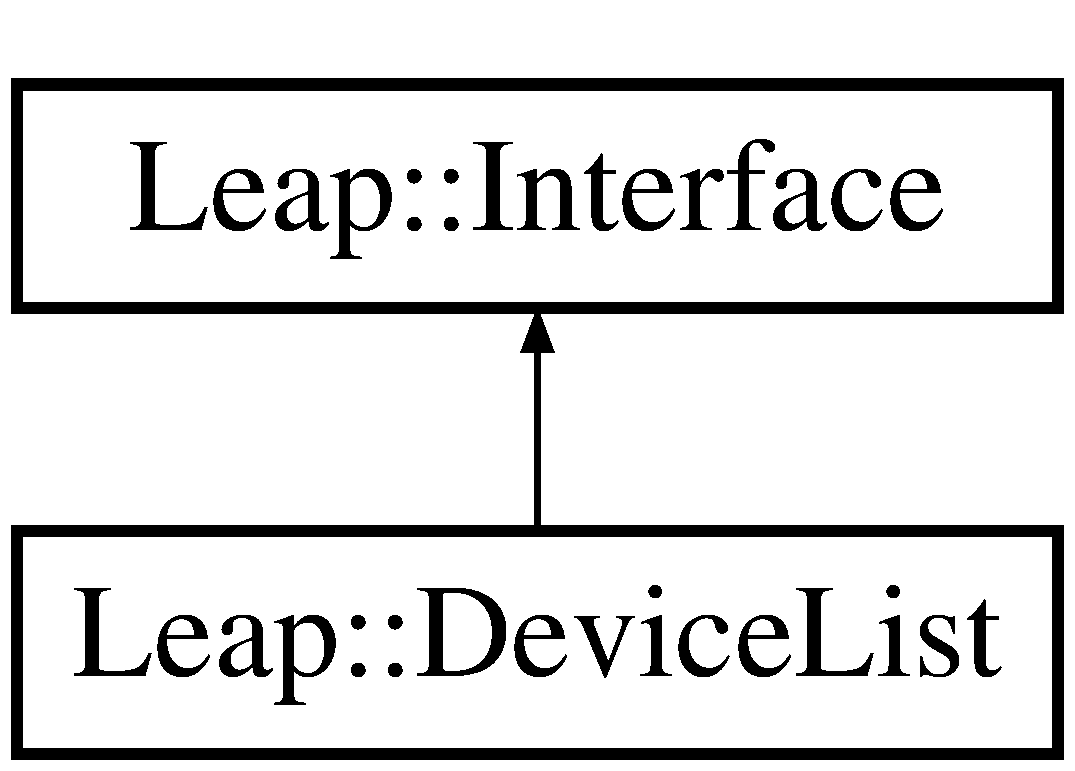
\includegraphics[height=2.000000cm]{class_leap_1_1_device_list}
\end{center}
\end{figure}
\subsection*{Public Types}
\begin{DoxyCompactItemize}
\item 
typedef \hyperlink{class_leap_1_1_const_list_iterator}{Const\+List\+Iterator}\\*
$<$ \hyperlink{class_leap_1_1_device_list}{Device\+List}, \hyperlink{class_leap_1_1_device}{Device} $>$ \hyperlink{class_leap_1_1_device_list_acfe5b07cda502759bf8fe768e8c6ba87}{const\+\_\+iterator}
\end{DoxyCompactItemize}
\subsection*{Public Member Functions}
\begin{DoxyCompactItemize}
\item 
\hypertarget{class_leap_1_1_device_list_a5526b7741f4a2689c330d34fc7a865db}{{\bfseries Device\+List} (const \hyperlink{class_leap_1_1_list_base_implementation}{List\+Base\+Implementation}$<$ \hyperlink{class_leap_1_1_device}{Device} $>$ \&)}\label{class_leap_1_1_device_list_a5526b7741f4a2689c330d34fc7a865db}

\item 
L\+E\+A\+P\+\_\+\+E\+X\+P\+O\+R\+T \hyperlink{class_leap_1_1_device_list_a6b438e4f4e9486c9d38e6ac01a9e7b93}{Device\+List} ()
\item 
L\+E\+A\+P\+\_\+\+E\+X\+P\+O\+R\+T int \hyperlink{class_leap_1_1_device_list_ad908f85b9d6282f4a898b743c4be3572}{count} () const 
\item 
L\+E\+A\+P\+\_\+\+E\+X\+P\+O\+R\+T bool \hyperlink{class_leap_1_1_device_list_abe9d868daf53da6fa412e19d64330684}{is\+Empty} () const 
\item 
L\+E\+A\+P\+\_\+\+E\+X\+P\+O\+R\+T \hyperlink{class_leap_1_1_device}{Device} \hyperlink{class_leap_1_1_device_list_a6719e35225afb3ddc9a1f303b273d831}{operator\mbox{[}$\,$\mbox{]}} (int index) const 
\item 
L\+E\+A\+P\+\_\+\+E\+X\+P\+O\+R\+T \hyperlink{class_leap_1_1_device_list}{Device\+List} \& \hyperlink{class_leap_1_1_device_list_aa5a6dd4fcc38029bfd381e34bcae4c43}{append} (const \hyperlink{class_leap_1_1_device_list}{Device\+List} \&other)
\item 
L\+E\+A\+P\+\_\+\+E\+X\+P\+O\+R\+T \hyperlink{class_leap_1_1_device_list_acfe5b07cda502759bf8fe768e8c6ba87}{const\+\_\+iterator} \hyperlink{class_leap_1_1_device_list_aa8743e646b1ba2ad7384153d67b01668}{begin} () const 
\item 
L\+E\+A\+P\+\_\+\+E\+X\+P\+O\+R\+T \hyperlink{class_leap_1_1_device_list_acfe5b07cda502759bf8fe768e8c6ba87}{const\+\_\+iterator} \hyperlink{class_leap_1_1_device_list_a6cf5deb1156da1b3af00c902ee170d67}{end} () const 
\end{DoxyCompactItemize}
\subsection*{Additional Inherited Members}


\subsection{Detailed Description}
The \hyperlink{class_leap_1_1_device_list}{Device\+List} class represents a list of \hyperlink{class_leap_1_1_device}{Device} objects.

Get a \hyperlink{class_leap_1_1_device_list}{Device\+List} object by calling \hyperlink{class_leap_1_1_controller_a5dc199cb8f41cf07724c494107744251}{Controller\+::devices()}. \begin{DoxySince}{Since}
1.\+0 
\end{DoxySince}


\subsection{Member Typedef Documentation}
\hypertarget{class_leap_1_1_device_list_acfe5b07cda502759bf8fe768e8c6ba87}{\index{Leap\+::\+Device\+List@{Leap\+::\+Device\+List}!const\+\_\+iterator@{const\+\_\+iterator}}
\index{const\+\_\+iterator@{const\+\_\+iterator}!Leap\+::\+Device\+List@{Leap\+::\+Device\+List}}
\subsubsection[{const\+\_\+iterator}]{\setlength{\rightskip}{0pt plus 5cm}typedef {\bf Const\+List\+Iterator}$<${\bf Device\+List}, {\bf Device}$>$ {\bf Leap\+::\+Device\+List\+::const\+\_\+iterator}}}\label{class_leap_1_1_device_list_acfe5b07cda502759bf8fe768e8c6ba87}
A C++ iterator type for this \hyperlink{class_leap_1_1_device_list}{Device\+List} objects. \begin{DoxySince}{Since}
1.\+0 
\end{DoxySince}


\subsection{Constructor \& Destructor Documentation}
\hypertarget{class_leap_1_1_device_list_a6b438e4f4e9486c9d38e6ac01a9e7b93}{\index{Leap\+::\+Device\+List@{Leap\+::\+Device\+List}!Device\+List@{Device\+List}}
\index{Device\+List@{Device\+List}!Leap\+::\+Device\+List@{Leap\+::\+Device\+List}}
\subsubsection[{Device\+List}]{\setlength{\rightskip}{0pt plus 5cm}L\+E\+A\+P\+\_\+\+E\+X\+P\+O\+R\+T Leap\+::\+Device\+List\+::\+Device\+List (
\begin{DoxyParamCaption}
{}
\end{DoxyParamCaption}
)}}\label{class_leap_1_1_device_list_a6b438e4f4e9486c9d38e6ac01a9e7b93}
Constructs an empty list of devices. \begin{DoxySince}{Since}
1.\+0 
\end{DoxySince}


\subsection{Member Function Documentation}
\hypertarget{class_leap_1_1_device_list_aa5a6dd4fcc38029bfd381e34bcae4c43}{\index{Leap\+::\+Device\+List@{Leap\+::\+Device\+List}!append@{append}}
\index{append@{append}!Leap\+::\+Device\+List@{Leap\+::\+Device\+List}}
\subsubsection[{append}]{\setlength{\rightskip}{0pt plus 5cm}L\+E\+A\+P\+\_\+\+E\+X\+P\+O\+R\+T {\bf Device\+List}\& Leap\+::\+Device\+List\+::append (
\begin{DoxyParamCaption}
\item[{const {\bf Device\+List} \&}]{other}
\end{DoxyParamCaption}
)}}\label{class_leap_1_1_device_list_aa5a6dd4fcc38029bfd381e34bcae4c43}
Appends the members of the specifed \hyperlink{class_leap_1_1_device_list}{Device\+List} to this \hyperlink{class_leap_1_1_device_list}{Device\+List}. 
\begin{DoxyParams}{Parameters}
{\em other} & A \hyperlink{class_leap_1_1_device_list}{Device\+List} object containing \hyperlink{class_leap_1_1_device}{Device} objects to append to the end of this \hyperlink{class_leap_1_1_device_list}{Device\+List}. \\
\hline
\end{DoxyParams}
\begin{DoxySince}{Since}
1.\+0 
\end{DoxySince}
\hypertarget{class_leap_1_1_device_list_aa8743e646b1ba2ad7384153d67b01668}{\index{Leap\+::\+Device\+List@{Leap\+::\+Device\+List}!begin@{begin}}
\index{begin@{begin}!Leap\+::\+Device\+List@{Leap\+::\+Device\+List}}
\subsubsection[{begin}]{\setlength{\rightskip}{0pt plus 5cm}L\+E\+A\+P\+\_\+\+E\+X\+P\+O\+R\+T {\bf const\+\_\+iterator} Leap\+::\+Device\+List\+::begin (
\begin{DoxyParamCaption}
{}
\end{DoxyParamCaption}
) const}}\label{class_leap_1_1_device_list_aa8743e646b1ba2ad7384153d67b01668}
The C++ iterator set to the beginning of this \hyperlink{class_leap_1_1_device_list}{Device\+List}. \begin{DoxySince}{Since}
1.\+0 
\end{DoxySince}
\hypertarget{class_leap_1_1_device_list_ad908f85b9d6282f4a898b743c4be3572}{\index{Leap\+::\+Device\+List@{Leap\+::\+Device\+List}!count@{count}}
\index{count@{count}!Leap\+::\+Device\+List@{Leap\+::\+Device\+List}}
\subsubsection[{count}]{\setlength{\rightskip}{0pt plus 5cm}L\+E\+A\+P\+\_\+\+E\+X\+P\+O\+R\+T int Leap\+::\+Device\+List\+::count (
\begin{DoxyParamCaption}
{}
\end{DoxyParamCaption}
) const}}\label{class_leap_1_1_device_list_ad908f85b9d6282f4a898b743c4be3572}
Returns the number of devices in this list. \begin{DoxyReturn}{Returns}
The number of devices in this list. 
\end{DoxyReturn}
\begin{DoxySince}{Since}
1.\+0 
\end{DoxySince}
\hypertarget{class_leap_1_1_device_list_a6cf5deb1156da1b3af00c902ee170d67}{\index{Leap\+::\+Device\+List@{Leap\+::\+Device\+List}!end@{end}}
\index{end@{end}!Leap\+::\+Device\+List@{Leap\+::\+Device\+List}}
\subsubsection[{end}]{\setlength{\rightskip}{0pt plus 5cm}L\+E\+A\+P\+\_\+\+E\+X\+P\+O\+R\+T {\bf const\+\_\+iterator} Leap\+::\+Device\+List\+::end (
\begin{DoxyParamCaption}
{}
\end{DoxyParamCaption}
) const}}\label{class_leap_1_1_device_list_a6cf5deb1156da1b3af00c902ee170d67}
The C++ iterator set to the end of this \hyperlink{class_leap_1_1_device_list}{Device\+List}. \begin{DoxySince}{Since}
1.\+0 
\end{DoxySince}
\hypertarget{class_leap_1_1_device_list_abe9d868daf53da6fa412e19d64330684}{\index{Leap\+::\+Device\+List@{Leap\+::\+Device\+List}!is\+Empty@{is\+Empty}}
\index{is\+Empty@{is\+Empty}!Leap\+::\+Device\+List@{Leap\+::\+Device\+List}}
\subsubsection[{is\+Empty}]{\setlength{\rightskip}{0pt plus 5cm}L\+E\+A\+P\+\_\+\+E\+X\+P\+O\+R\+T bool Leap\+::\+Device\+List\+::is\+Empty (
\begin{DoxyParamCaption}
{}
\end{DoxyParamCaption}
) const}}\label{class_leap_1_1_device_list_abe9d868daf53da6fa412e19d64330684}
Reports whether the list is empty. \begin{DoxyReturn}{Returns}
True, if the list has no members. 
\end{DoxyReturn}
\begin{DoxySince}{Since}
1.\+0 
\end{DoxySince}
\hypertarget{class_leap_1_1_device_list_a6719e35225afb3ddc9a1f303b273d831}{\index{Leap\+::\+Device\+List@{Leap\+::\+Device\+List}!operator\mbox{[}$\,$\mbox{]}@{operator[]}}
\index{operator\mbox{[}$\,$\mbox{]}@{operator[]}!Leap\+::\+Device\+List@{Leap\+::\+Device\+List}}
\subsubsection[{operator[]}]{\setlength{\rightskip}{0pt plus 5cm}L\+E\+A\+P\+\_\+\+E\+X\+P\+O\+R\+T {\bf Device} Leap\+::\+Device\+List\+::operator\mbox{[}$\,$\mbox{]} (
\begin{DoxyParamCaption}
\item[{int}]{index}
\end{DoxyParamCaption}
) const}}\label{class_leap_1_1_device_list_a6719e35225afb3ddc9a1f303b273d831}
Access a list member by its position in the list. 
\begin{DoxyParams}{Parameters}
{\em index} & The zero-\/based list position index. \\
\hline
\end{DoxyParams}
\begin{DoxyReturn}{Returns}
The \hyperlink{class_leap_1_1_device}{Device} object at the specified index. 
\end{DoxyReturn}
\begin{DoxySince}{Since}
1.\+0 
\end{DoxySince}


The documentation for this class was generated from the following file\+:\begin{DoxyCompactItemize}
\item 
Interface\+Managers/Leap.\+h\end{DoxyCompactItemize}

\hypertarget{class_event_listener}{\section{Event\+Listener Class Reference}
\label{class_event_listener}\index{Event\+Listener@{Event\+Listener}}
}


{\ttfamily \#include $<$eventlistener.\+h$>$}

Inheritance diagram for Event\+Listener\+:\begin{figure}[H]
\begin{center}
\leavevmode
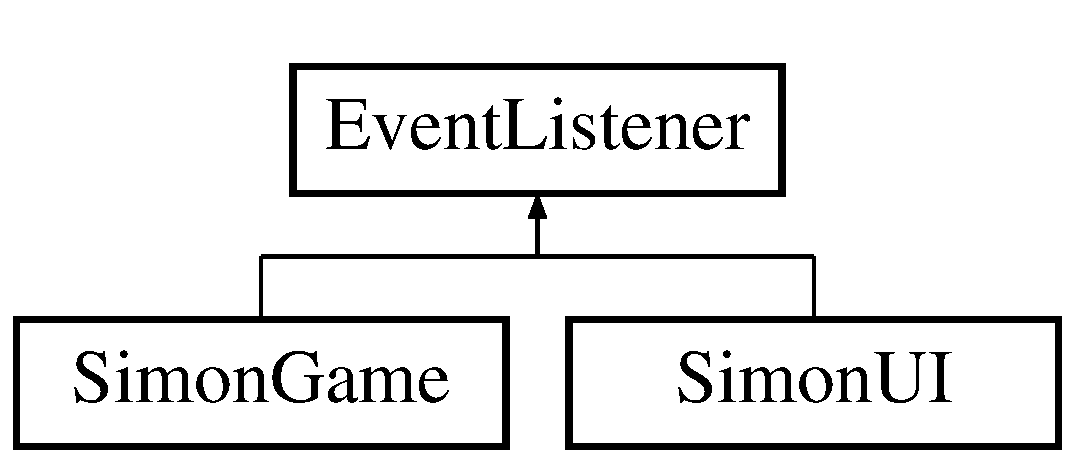
\includegraphics[height=2.000000cm]{class_event_listener}
\end{center}
\end{figure}
\subsection*{Public Member Functions}
\begin{DoxyCompactItemize}
\item 
virtual \hyperlink{class_event_listener_ad03c1e6f45e92434d502995a4f31685e}{$\sim$\+Event\+Listener} ()
\item 
virtual void \hyperlink{class_event_listener_a19232875c793366beb4d8edb0cc89164}{on\+Event} (Quadrant\+I\+D, Event\+Type)
\end{DoxyCompactItemize}


\subsection{Detailed Description}
An abstract class for event listeners 

\subsection{Constructor \& Destructor Documentation}
\hypertarget{class_event_listener_ad03c1e6f45e92434d502995a4f31685e}{\index{Event\+Listener@{Event\+Listener}!````~Event\+Listener@{$\sim$\+Event\+Listener}}
\index{````~Event\+Listener@{$\sim$\+Event\+Listener}!Event\+Listener@{Event\+Listener}}
\subsubsection[{$\sim$\+Event\+Listener}]{\setlength{\rightskip}{0pt plus 5cm}virtual Event\+Listener\+::$\sim$\+Event\+Listener (
\begin{DoxyParamCaption}
{}
\end{DoxyParamCaption}
)\hspace{0.3cm}{\ttfamily [inline]}, {\ttfamily [virtual]}}}\label{class_event_listener_ad03c1e6f45e92434d502995a4f31685e}
Virtual destructor 

\subsection{Member Function Documentation}
\hypertarget{class_event_listener_a19232875c793366beb4d8edb0cc89164}{\index{Event\+Listener@{Event\+Listener}!on\+Event@{on\+Event}}
\index{on\+Event@{on\+Event}!Event\+Listener@{Event\+Listener}}
\subsubsection[{on\+Event}]{\setlength{\rightskip}{0pt plus 5cm}virtual void Event\+Listener\+::on\+Event (
\begin{DoxyParamCaption}
\item[{Quadrant\+I\+D}]{, }
\item[{Event\+Type}]{}
\end{DoxyParamCaption}
)\hspace{0.3cm}{\ttfamily [inline]}, {\ttfamily [virtual]}}}\label{class_event_listener_a19232875c793366beb4d8edb0cc89164}
Fired when an event occurs with an input device 

Reimplemented in \hyperlink{class_simon_game_a35dc2ba138666e626ef663ef6b954f4b}{Simon\+Game}, and \hyperlink{class_simon_u_i_a9a8de04376322efe03495a873d8e08d9}{Simon\+U\+I}.



The documentation for this class was generated from the following file\+:\begin{DoxyCompactItemize}
\item 
Interface\+Managers/eventlistener.\+h\end{DoxyCompactItemize}

\hypertarget{class_leap_1_1_finger}{\section{Leap\+:\+:Finger Class Reference}
\label{class_leap_1_1_finger}\index{Leap\+::\+Finger@{Leap\+::\+Finger}}
}


{\ttfamily \#include $<$Leap.\+h$>$}

Inheritance diagram for Leap\+:\+:Finger\+:\begin{figure}[H]
\begin{center}
\leavevmode
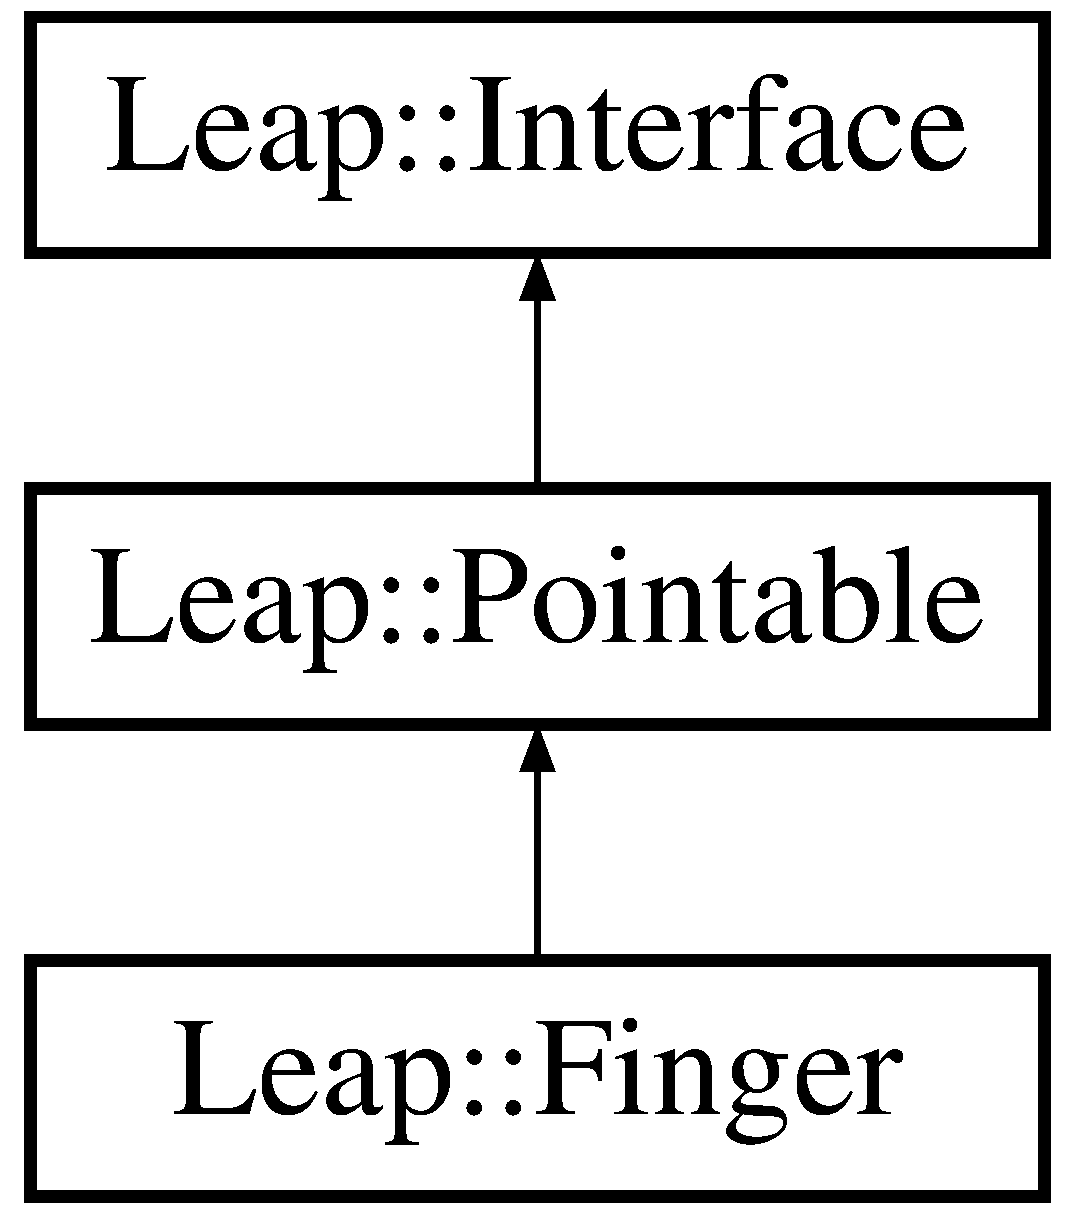
\includegraphics[height=3.000000cm]{class_leap_1_1_finger}
\end{center}
\end{figure}
\subsection*{Public Member Functions}
\begin{DoxyCompactItemize}
\item 
\hypertarget{class_leap_1_1_finger_ac393e4d718a2163fabd65b85d5c09267}{{\bfseries Finger} (Finger\+Implementation $\ast$)}\label{class_leap_1_1_finger_ac393e4d718a2163fabd65b85d5c09267}

\item 
L\+E\+A\+P\+\_\+\+E\+X\+P\+O\+R\+T \hyperlink{class_leap_1_1_finger_aed76c909a2904029d313538e01604c88}{Finger} ()
\item 
L\+E\+A\+P\+\_\+\+E\+X\+P\+O\+R\+T \hyperlink{class_leap_1_1_finger_a864d7de003b2d5b6d738c67da322e702}{Finger} (const \hyperlink{class_leap_1_1_pointable}{Pointable} \&)
\item 
L\+E\+A\+P\+\_\+\+E\+X\+P\+O\+R\+T std\+::string \hyperlink{class_leap_1_1_finger_a2641934432be97ad3c33c8dbe287a7b9}{to\+String} () const 
\end{DoxyCompactItemize}
\subsection*{Static Public Member Functions}
\begin{DoxyCompactItemize}
\item 
static L\+E\+A\+P\+\_\+\+E\+X\+P\+O\+R\+T const \hyperlink{class_leap_1_1_finger}{Finger} \& \hyperlink{class_leap_1_1_finger_a2dec17262f38e1bb548da99086c5e8e3}{invalid} ()
\end{DoxyCompactItemize}
\subsection*{Additional Inherited Members}


\subsection{Detailed Description}
The \hyperlink{class_leap_1_1_finger}{Finger} class represents a tracked finger.

Fingers are \hyperlink{class_leap_1_1_pointable}{Pointable} objects that the Leap Motion software has classified as a finger. Get valid \hyperlink{class_leap_1_1_finger}{Finger} objects from a \hyperlink{class_leap_1_1_frame}{Frame} or a \hyperlink{class_leap_1_1_hand}{Hand} object.

Fingers may be permanently associated to a hand. In this case the angular order of the finger I\+Ds will be invariant. As fingers move in and out of view it is possible for the guessed I\+D of a finger to be incorrect. Consequently, it may be necessary for finger I\+Ds to be exchanged. All tracked properties, such as velocity, will remain continuous in the A\+P\+I. However, quantities that are derived from the A\+P\+I output (such as a history of positions) will be discontinuous unless they have a corresponding I\+D exchange.

Note that \hyperlink{class_leap_1_1_finger}{Finger} objects can be invalid, which means that they do not contain valid tracking data and do not correspond to a physical finger. Invalid \hyperlink{class_leap_1_1_finger}{Finger} objects can be the result of asking for a \hyperlink{class_leap_1_1_finger}{Finger} object using an I\+D from an earlier frame when no \hyperlink{class_leap_1_1_finger}{Finger} objects with that I\+D exist in the current frame. A \hyperlink{class_leap_1_1_finger}{Finger} object created from the \hyperlink{class_leap_1_1_finger}{Finger} constructor is also invalid. Test for validity with the \hyperlink{class_leap_1_1_pointable_a124f21a619df4fb338d1ce8a7a6d3341}{Finger\+::is\+Valid()} function. \begin{DoxySince}{Since}
1.\+0 
\end{DoxySince}


\subsection{Constructor \& Destructor Documentation}
\hypertarget{class_leap_1_1_finger_aed76c909a2904029d313538e01604c88}{\index{Leap\+::\+Finger@{Leap\+::\+Finger}!Finger@{Finger}}
\index{Finger@{Finger}!Leap\+::\+Finger@{Leap\+::\+Finger}}
\subsubsection[{Finger}]{\setlength{\rightskip}{0pt plus 5cm}L\+E\+A\+P\+\_\+\+E\+X\+P\+O\+R\+T Leap\+::\+Finger\+::\+Finger (
\begin{DoxyParamCaption}
{}
\end{DoxyParamCaption}
)}}\label{class_leap_1_1_finger_aed76c909a2904029d313538e01604c88}
Constructs a \hyperlink{class_leap_1_1_finger}{Finger} object.

An uninitialized finger is considered invalid. Get valid \hyperlink{class_leap_1_1_finger}{Finger} objects from a \hyperlink{class_leap_1_1_frame}{Frame} or a \hyperlink{class_leap_1_1_hand}{Hand} object. \begin{DoxySince}{Since}
1.\+0 
\end{DoxySince}
\hypertarget{class_leap_1_1_finger_a864d7de003b2d5b6d738c67da322e702}{\index{Leap\+::\+Finger@{Leap\+::\+Finger}!Finger@{Finger}}
\index{Finger@{Finger}!Leap\+::\+Finger@{Leap\+::\+Finger}}
\subsubsection[{Finger}]{\setlength{\rightskip}{0pt plus 5cm}L\+E\+A\+P\+\_\+\+E\+X\+P\+O\+R\+T Leap\+::\+Finger\+::\+Finger (
\begin{DoxyParamCaption}
\item[{const {\bf Pointable} \&}]{}
\end{DoxyParamCaption}
)\hspace{0.3cm}{\ttfamily [explicit]}}}\label{class_leap_1_1_finger_a864d7de003b2d5b6d738c67da322e702}
If the specified \hyperlink{class_leap_1_1_pointable}{Pointable} object represents a finger, creates a copy of it as a \hyperlink{class_leap_1_1_finger}{Finger} object; otherwise, creates an invalid \hyperlink{class_leap_1_1_finger}{Finger} object. \begin{DoxySince}{Since}
1.\+0 
\end{DoxySince}


\subsection{Member Function Documentation}
\hypertarget{class_leap_1_1_finger_a2dec17262f38e1bb548da99086c5e8e3}{\index{Leap\+::\+Finger@{Leap\+::\+Finger}!invalid@{invalid}}
\index{invalid@{invalid}!Leap\+::\+Finger@{Leap\+::\+Finger}}
\subsubsection[{invalid}]{\setlength{\rightskip}{0pt plus 5cm}static L\+E\+A\+P\+\_\+\+E\+X\+P\+O\+R\+T const {\bf Finger}\& Leap\+::\+Finger\+::invalid (
\begin{DoxyParamCaption}
{}
\end{DoxyParamCaption}
)\hspace{0.3cm}{\ttfamily [static]}}}\label{class_leap_1_1_finger_a2dec17262f38e1bb548da99086c5e8e3}
Returns an invalid \hyperlink{class_leap_1_1_finger}{Finger} object.

You can use the instance returned by this function in comparisons testing whether a given \hyperlink{class_leap_1_1_finger}{Finger} instance is valid or invalid. (You can also use the \hyperlink{class_leap_1_1_pointable_a124f21a619df4fb338d1ce8a7a6d3341}{Finger\+::is\+Valid()} function.)

\begin{DoxyReturn}{Returns}
The invalid \hyperlink{class_leap_1_1_finger}{Finger} instance. 
\end{DoxyReturn}
\begin{DoxySince}{Since}
1.\+0 
\end{DoxySince}
\hypertarget{class_leap_1_1_finger_a2641934432be97ad3c33c8dbe287a7b9}{\index{Leap\+::\+Finger@{Leap\+::\+Finger}!to\+String@{to\+String}}
\index{to\+String@{to\+String}!Leap\+::\+Finger@{Leap\+::\+Finger}}
\subsubsection[{to\+String}]{\setlength{\rightskip}{0pt plus 5cm}L\+E\+A\+P\+\_\+\+E\+X\+P\+O\+R\+T std\+::string Leap\+::\+Finger\+::to\+String (
\begin{DoxyParamCaption}
{}
\end{DoxyParamCaption}
) const}}\label{class_leap_1_1_finger_a2641934432be97ad3c33c8dbe287a7b9}
A string containing a brief, human readable description of the \hyperlink{class_leap_1_1_finger}{Finger} object.

\begin{DoxyReturn}{Returns}
A description of the \hyperlink{class_leap_1_1_finger}{Finger} object as a string. 
\end{DoxyReturn}
\begin{DoxySince}{Since}
1.\+0 
\end{DoxySince}


The documentation for this class was generated from the following file\+:\begin{DoxyCompactItemize}
\item 
Interface\+Managers/Leap.\+h\end{DoxyCompactItemize}

\hypertarget{class_leap_1_1_finger_list}{\section{Leap\+:\+:Finger\+List Class Reference}
\label{class_leap_1_1_finger_list}\index{Leap\+::\+Finger\+List@{Leap\+::\+Finger\+List}}
}


{\ttfamily \#include $<$Leap.\+h$>$}

Inheritance diagram for Leap\+:\+:Finger\+List\+:\begin{figure}[H]
\begin{center}
\leavevmode
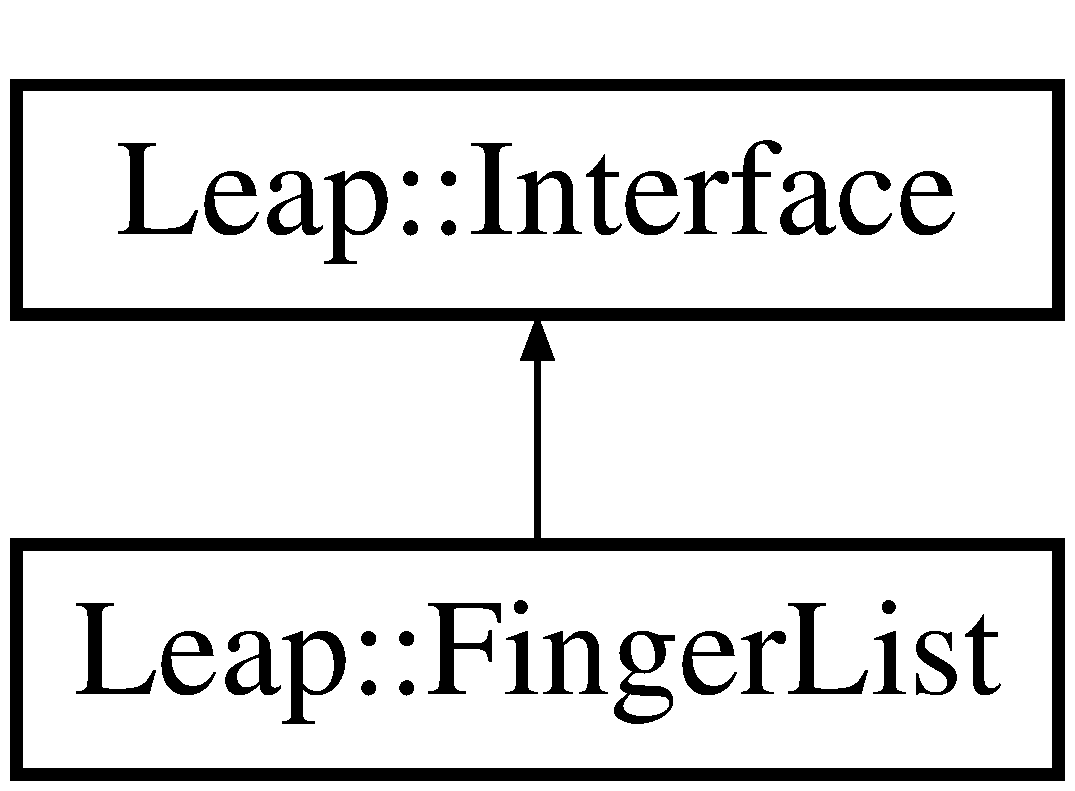
\includegraphics[height=2.000000cm]{class_leap_1_1_finger_list}
\end{center}
\end{figure}
\subsection*{Public Types}
\begin{DoxyCompactItemize}
\item 
typedef \hyperlink{class_leap_1_1_const_list_iterator}{Const\+List\+Iterator}\\*
$<$ \hyperlink{class_leap_1_1_finger_list}{Finger\+List}, \hyperlink{class_leap_1_1_finger}{Finger} $>$ \hyperlink{class_leap_1_1_finger_list_a9ecff6e555096064a09bb66a8cb5e567}{const\+\_\+iterator}
\end{DoxyCompactItemize}
\subsection*{Public Member Functions}
\begin{DoxyCompactItemize}
\item 
\hypertarget{class_leap_1_1_finger_list_a730629d5b27f07888ddb574bf06a85ef}{{\bfseries Finger\+List} (const \hyperlink{class_leap_1_1_list_base_implementation}{List\+Base\+Implementation}$<$ \hyperlink{class_leap_1_1_finger}{Finger} $>$ \&)}\label{class_leap_1_1_finger_list_a730629d5b27f07888ddb574bf06a85ef}

\item 
L\+E\+A\+P\+\_\+\+E\+X\+P\+O\+R\+T \hyperlink{class_leap_1_1_finger_list_aa04009715ecbb8b2417a1459ed3bb7fd}{Finger\+List} ()
\item 
L\+E\+A\+P\+\_\+\+E\+X\+P\+O\+R\+T int \hyperlink{class_leap_1_1_finger_list_aaa09782751e73f39e750b2546c540890}{count} () const 
\item 
L\+E\+A\+P\+\_\+\+E\+X\+P\+O\+R\+T bool \hyperlink{class_leap_1_1_finger_list_a9c44f0e3dad3efd67e4135b96976ed7f}{is\+Empty} () const 
\item 
L\+E\+A\+P\+\_\+\+E\+X\+P\+O\+R\+T \hyperlink{class_leap_1_1_finger}{Finger} \hyperlink{class_leap_1_1_finger_list_a61a359916561b6bc3b7be011f1c945cd}{operator\mbox{[}$\,$\mbox{]}} (int index) const 
\item 
L\+E\+A\+P\+\_\+\+E\+X\+P\+O\+R\+T \hyperlink{class_leap_1_1_finger_list}{Finger\+List} \& \hyperlink{class_leap_1_1_finger_list_ab032377473c269651a1110f3a5de3263}{append} (const \hyperlink{class_leap_1_1_finger_list}{Finger\+List} \&other)
\item 
L\+E\+A\+P\+\_\+\+E\+X\+P\+O\+R\+T \hyperlink{class_leap_1_1_finger}{Finger} \hyperlink{class_leap_1_1_finger_list_aa236b4cf2b2e0fc7bb4760eed44d2e17}{leftmost} () const 
\item 
L\+E\+A\+P\+\_\+\+E\+X\+P\+O\+R\+T \hyperlink{class_leap_1_1_finger}{Finger} \hyperlink{class_leap_1_1_finger_list_a9259519d48339344503fe36814084d7e}{rightmost} () const 
\item 
L\+E\+A\+P\+\_\+\+E\+X\+P\+O\+R\+T \hyperlink{class_leap_1_1_finger}{Finger} \hyperlink{class_leap_1_1_finger_list_af3e57d0957d58438269f713519fec60a}{frontmost} () const 
\item 
L\+E\+A\+P\+\_\+\+E\+X\+P\+O\+R\+T \hyperlink{class_leap_1_1_finger_list_a9ecff6e555096064a09bb66a8cb5e567}{const\+\_\+iterator} \hyperlink{class_leap_1_1_finger_list_adde4cf74c2836822b967d07ad51848cb}{begin} () const 
\item 
L\+E\+A\+P\+\_\+\+E\+X\+P\+O\+R\+T \hyperlink{class_leap_1_1_finger_list_a9ecff6e555096064a09bb66a8cb5e567}{const\+\_\+iterator} \hyperlink{class_leap_1_1_finger_list_a31f0d3b78f4257f5ffd5353b30ce894a}{end} () const 
\end{DoxyCompactItemize}
\subsection*{Additional Inherited Members}


\subsection{Detailed Description}
The \hyperlink{class_leap_1_1_finger_list}{Finger\+List} class represents a list of \hyperlink{class_leap_1_1_finger}{Finger} objects.

Get a \hyperlink{class_leap_1_1_finger_list}{Finger\+List} object by calling \hyperlink{class_leap_1_1_frame_abff33c86515d42793abf134e359e5142}{Frame\+::fingers()}. \begin{DoxySince}{Since}
1.\+0 
\end{DoxySince}


\subsection{Member Typedef Documentation}
\hypertarget{class_leap_1_1_finger_list_a9ecff6e555096064a09bb66a8cb5e567}{\index{Leap\+::\+Finger\+List@{Leap\+::\+Finger\+List}!const\+\_\+iterator@{const\+\_\+iterator}}
\index{const\+\_\+iterator@{const\+\_\+iterator}!Leap\+::\+Finger\+List@{Leap\+::\+Finger\+List}}
\subsubsection[{const\+\_\+iterator}]{\setlength{\rightskip}{0pt plus 5cm}typedef {\bf Const\+List\+Iterator}$<${\bf Finger\+List}, {\bf Finger}$>$ {\bf Leap\+::\+Finger\+List\+::const\+\_\+iterator}}}\label{class_leap_1_1_finger_list_a9ecff6e555096064a09bb66a8cb5e567}
A C++ iterator type for \hyperlink{class_leap_1_1_finger_list}{Finger\+List} objects. \begin{DoxySince}{Since}
1.\+0 
\end{DoxySince}


\subsection{Constructor \& Destructor Documentation}
\hypertarget{class_leap_1_1_finger_list_aa04009715ecbb8b2417a1459ed3bb7fd}{\index{Leap\+::\+Finger\+List@{Leap\+::\+Finger\+List}!Finger\+List@{Finger\+List}}
\index{Finger\+List@{Finger\+List}!Leap\+::\+Finger\+List@{Leap\+::\+Finger\+List}}
\subsubsection[{Finger\+List}]{\setlength{\rightskip}{0pt plus 5cm}L\+E\+A\+P\+\_\+\+E\+X\+P\+O\+R\+T Leap\+::\+Finger\+List\+::\+Finger\+List (
\begin{DoxyParamCaption}
{}
\end{DoxyParamCaption}
)}}\label{class_leap_1_1_finger_list_aa04009715ecbb8b2417a1459ed3bb7fd}
Constructs an empty list of fingers. \begin{DoxySince}{Since}
1.\+0 
\end{DoxySince}


\subsection{Member Function Documentation}
\hypertarget{class_leap_1_1_finger_list_ab032377473c269651a1110f3a5de3263}{\index{Leap\+::\+Finger\+List@{Leap\+::\+Finger\+List}!append@{append}}
\index{append@{append}!Leap\+::\+Finger\+List@{Leap\+::\+Finger\+List}}
\subsubsection[{append}]{\setlength{\rightskip}{0pt plus 5cm}L\+E\+A\+P\+\_\+\+E\+X\+P\+O\+R\+T {\bf Finger\+List}\& Leap\+::\+Finger\+List\+::append (
\begin{DoxyParamCaption}
\item[{const {\bf Finger\+List} \&}]{other}
\end{DoxyParamCaption}
)}}\label{class_leap_1_1_finger_list_ab032377473c269651a1110f3a5de3263}
Appends the members of the specifed \hyperlink{class_leap_1_1_finger_list}{Finger\+List} to this \hyperlink{class_leap_1_1_finger_list}{Finger\+List}. 
\begin{DoxyParams}{Parameters}
{\em other} & A \hyperlink{class_leap_1_1_finger_list}{Finger\+List} object containing \hyperlink{class_leap_1_1_finger}{Finger} objects to append to the end of this \hyperlink{class_leap_1_1_finger_list}{Finger\+List}. \\
\hline
\end{DoxyParams}
\begin{DoxySince}{Since}
1.\+0 
\end{DoxySince}
\hypertarget{class_leap_1_1_finger_list_adde4cf74c2836822b967d07ad51848cb}{\index{Leap\+::\+Finger\+List@{Leap\+::\+Finger\+List}!begin@{begin}}
\index{begin@{begin}!Leap\+::\+Finger\+List@{Leap\+::\+Finger\+List}}
\subsubsection[{begin}]{\setlength{\rightskip}{0pt plus 5cm}L\+E\+A\+P\+\_\+\+E\+X\+P\+O\+R\+T {\bf const\+\_\+iterator} Leap\+::\+Finger\+List\+::begin (
\begin{DoxyParamCaption}
{}
\end{DoxyParamCaption}
) const}}\label{class_leap_1_1_finger_list_adde4cf74c2836822b967d07ad51848cb}
The C++ iterator set to the beginning of this \hyperlink{class_leap_1_1_finger_list}{Finger\+List}. \begin{DoxySince}{Since}
1.\+0 
\end{DoxySince}
\hypertarget{class_leap_1_1_finger_list_aaa09782751e73f39e750b2546c540890}{\index{Leap\+::\+Finger\+List@{Leap\+::\+Finger\+List}!count@{count}}
\index{count@{count}!Leap\+::\+Finger\+List@{Leap\+::\+Finger\+List}}
\subsubsection[{count}]{\setlength{\rightskip}{0pt plus 5cm}L\+E\+A\+P\+\_\+\+E\+X\+P\+O\+R\+T int Leap\+::\+Finger\+List\+::count (
\begin{DoxyParamCaption}
{}
\end{DoxyParamCaption}
) const}}\label{class_leap_1_1_finger_list_aaa09782751e73f39e750b2546c540890}
Returns the number of fingers in this list. \begin{DoxyReturn}{Returns}
The number of fingers in this list. 
\end{DoxyReturn}
\begin{DoxySince}{Since}
1.\+0 
\end{DoxySince}
\hypertarget{class_leap_1_1_finger_list_a31f0d3b78f4257f5ffd5353b30ce894a}{\index{Leap\+::\+Finger\+List@{Leap\+::\+Finger\+List}!end@{end}}
\index{end@{end}!Leap\+::\+Finger\+List@{Leap\+::\+Finger\+List}}
\subsubsection[{end}]{\setlength{\rightskip}{0pt plus 5cm}L\+E\+A\+P\+\_\+\+E\+X\+P\+O\+R\+T {\bf const\+\_\+iterator} Leap\+::\+Finger\+List\+::end (
\begin{DoxyParamCaption}
{}
\end{DoxyParamCaption}
) const}}\label{class_leap_1_1_finger_list_a31f0d3b78f4257f5ffd5353b30ce894a}
The C++ iterator set to the end of this \hyperlink{class_leap_1_1_finger_list}{Finger\+List}. \begin{DoxySince}{Since}
1.\+0 
\end{DoxySince}
\hypertarget{class_leap_1_1_finger_list_af3e57d0957d58438269f713519fec60a}{\index{Leap\+::\+Finger\+List@{Leap\+::\+Finger\+List}!frontmost@{frontmost}}
\index{frontmost@{frontmost}!Leap\+::\+Finger\+List@{Leap\+::\+Finger\+List}}
\subsubsection[{frontmost}]{\setlength{\rightskip}{0pt plus 5cm}L\+E\+A\+P\+\_\+\+E\+X\+P\+O\+R\+T {\bf Finger} Leap\+::\+Finger\+List\+::frontmost (
\begin{DoxyParamCaption}
{}
\end{DoxyParamCaption}
) const}}\label{class_leap_1_1_finger_list_af3e57d0957d58438269f713519fec60a}
The member of the list that is farthest to the front within the standard Leap Motion frame of reference (i.\+e has the smallest Z coordinate).

\begin{DoxyReturn}{Returns}
The frontmost finger, or invalid if list is empty. 
\end{DoxyReturn}
\begin{DoxySince}{Since}
1.\+0 
\end{DoxySince}
\hypertarget{class_leap_1_1_finger_list_a9c44f0e3dad3efd67e4135b96976ed7f}{\index{Leap\+::\+Finger\+List@{Leap\+::\+Finger\+List}!is\+Empty@{is\+Empty}}
\index{is\+Empty@{is\+Empty}!Leap\+::\+Finger\+List@{Leap\+::\+Finger\+List}}
\subsubsection[{is\+Empty}]{\setlength{\rightskip}{0pt plus 5cm}L\+E\+A\+P\+\_\+\+E\+X\+P\+O\+R\+T bool Leap\+::\+Finger\+List\+::is\+Empty (
\begin{DoxyParamCaption}
{}
\end{DoxyParamCaption}
) const}}\label{class_leap_1_1_finger_list_a9c44f0e3dad3efd67e4135b96976ed7f}
Reports whether the list is empty. \begin{DoxyReturn}{Returns}
True, if the list has no members. 
\end{DoxyReturn}
\begin{DoxySince}{Since}
1.\+0 
\end{DoxySince}
\hypertarget{class_leap_1_1_finger_list_aa236b4cf2b2e0fc7bb4760eed44d2e17}{\index{Leap\+::\+Finger\+List@{Leap\+::\+Finger\+List}!leftmost@{leftmost}}
\index{leftmost@{leftmost}!Leap\+::\+Finger\+List@{Leap\+::\+Finger\+List}}
\subsubsection[{leftmost}]{\setlength{\rightskip}{0pt plus 5cm}L\+E\+A\+P\+\_\+\+E\+X\+P\+O\+R\+T {\bf Finger} Leap\+::\+Finger\+List\+::leftmost (
\begin{DoxyParamCaption}
{}
\end{DoxyParamCaption}
) const}}\label{class_leap_1_1_finger_list_aa236b4cf2b2e0fc7bb4760eed44d2e17}
The member of the list that is farthest to the left within the standard Leap Motion frame of reference (i.\+e has the smallest X coordinate).

\begin{DoxyReturn}{Returns}
The leftmost finger, or invalid if list is empty. 
\end{DoxyReturn}
\begin{DoxySince}{Since}
1.\+0 
\end{DoxySince}
\hypertarget{class_leap_1_1_finger_list_a61a359916561b6bc3b7be011f1c945cd}{\index{Leap\+::\+Finger\+List@{Leap\+::\+Finger\+List}!operator\mbox{[}$\,$\mbox{]}@{operator[]}}
\index{operator\mbox{[}$\,$\mbox{]}@{operator[]}!Leap\+::\+Finger\+List@{Leap\+::\+Finger\+List}}
\subsubsection[{operator[]}]{\setlength{\rightskip}{0pt plus 5cm}L\+E\+A\+P\+\_\+\+E\+X\+P\+O\+R\+T {\bf Finger} Leap\+::\+Finger\+List\+::operator\mbox{[}$\,$\mbox{]} (
\begin{DoxyParamCaption}
\item[{int}]{index}
\end{DoxyParamCaption}
) const}}\label{class_leap_1_1_finger_list_a61a359916561b6bc3b7be011f1c945cd}
Access a list member by its position in the list. 
\begin{DoxyParams}{Parameters}
{\em index} & The zero-\/based list position index. \\
\hline
\end{DoxyParams}
\begin{DoxyReturn}{Returns}
The \hyperlink{class_leap_1_1_finger}{Finger} object at the specified index. 
\end{DoxyReturn}
\begin{DoxySince}{Since}
1.\+0 
\end{DoxySince}
\hypertarget{class_leap_1_1_finger_list_a9259519d48339344503fe36814084d7e}{\index{Leap\+::\+Finger\+List@{Leap\+::\+Finger\+List}!rightmost@{rightmost}}
\index{rightmost@{rightmost}!Leap\+::\+Finger\+List@{Leap\+::\+Finger\+List}}
\subsubsection[{rightmost}]{\setlength{\rightskip}{0pt plus 5cm}L\+E\+A\+P\+\_\+\+E\+X\+P\+O\+R\+T {\bf Finger} Leap\+::\+Finger\+List\+::rightmost (
\begin{DoxyParamCaption}
{}
\end{DoxyParamCaption}
) const}}\label{class_leap_1_1_finger_list_a9259519d48339344503fe36814084d7e}
The member of the list that is farthest to the right within the standard Leap Motion frame of reference (i.\+e has the largest X coordinate).

\begin{DoxyReturn}{Returns}
The rightmost finger, or invalid if list is empty. 
\end{DoxyReturn}
\begin{DoxySince}{Since}
1.\+0 
\end{DoxySince}


The documentation for this class was generated from the following file\+:\begin{DoxyCompactItemize}
\item 
Interface\+Managers/Leap.\+h\end{DoxyCompactItemize}

\hypertarget{struct_leap_1_1_float_array}{\section{Leap\+:\+:Float\+Array Struct Reference}
\label{struct_leap_1_1_float_array}\index{Leap\+::\+Float\+Array@{Leap\+::\+Float\+Array}}
}


{\ttfamily \#include $<$Leap\+Math.\+h$>$}

\subsection*{Public Member Functions}
\begin{DoxyCompactItemize}
\item 
float \& \hyperlink{struct_leap_1_1_float_array_a9c4977609b3c6026fa9fd9091de35c1d}{operator\mbox{[}$\,$\mbox{]}} (unsigned int index)
\item 
\hyperlink{struct_leap_1_1_float_array_ad2e74b6ec198761806cc2d3c8bd28c74}{operator float $\ast$} ()
\item 
\hyperlink{struct_leap_1_1_float_array_ad71bfc9b61769596df36d38b5db365e6}{operator const float $\ast$} () const 
\end{DoxyCompactItemize}
\subsection*{Public Attributes}
\begin{DoxyCompactItemize}
\item 
float \hyperlink{struct_leap_1_1_float_array_a6f3a08d99f887c2f7afeb90955565a90}{m\+\_\+array} \mbox{[}16\mbox{]}
\end{DoxyCompactItemize}


\subsection{Detailed Description}
The \hyperlink{struct_leap_1_1_float_array}{Float\+Array} struct is used to allow the returning of native float arrays without requiring dynamic memory allocation. It represents a matrix with a size up to 4x4. \begin{DoxySince}{Since}
1.\+0 
\end{DoxySince}


\subsection{Member Function Documentation}
\hypertarget{struct_leap_1_1_float_array_ad71bfc9b61769596df36d38b5db365e6}{\index{Leap\+::\+Float\+Array@{Leap\+::\+Float\+Array}!operator const float $\ast$@{operator const float $\ast$}}
\index{operator const float $\ast$@{operator const float $\ast$}!Leap\+::\+Float\+Array@{Leap\+::\+Float\+Array}}
\subsubsection[{operator const float $\ast$}]{\setlength{\rightskip}{0pt plus 5cm}Leap\+::\+Float\+Array\+::operator const float $\ast$ (
\begin{DoxyParamCaption}
{}
\end{DoxyParamCaption}
) const\hspace{0.3cm}{\ttfamily [inline]}}}\label{struct_leap_1_1_float_array_ad71bfc9b61769596df36d38b5db365e6}
Use the Float Array anywhere a const float pointer can be used. \begin{DoxySince}{Since}
1.\+0 
\end{DoxySince}
\hypertarget{struct_leap_1_1_float_array_ad2e74b6ec198761806cc2d3c8bd28c74}{\index{Leap\+::\+Float\+Array@{Leap\+::\+Float\+Array}!operator float $\ast$@{operator float $\ast$}}
\index{operator float $\ast$@{operator float $\ast$}!Leap\+::\+Float\+Array@{Leap\+::\+Float\+Array}}
\subsubsection[{operator float $\ast$}]{\setlength{\rightskip}{0pt plus 5cm}Leap\+::\+Float\+Array\+::operator float $\ast$ (
\begin{DoxyParamCaption}
{}
\end{DoxyParamCaption}
)\hspace{0.3cm}{\ttfamily [inline]}}}\label{struct_leap_1_1_float_array_ad2e74b6ec198761806cc2d3c8bd28c74}
Use the Float Array anywhere a float pointer can be used. \begin{DoxySince}{Since}
1.\+0 
\end{DoxySince}
\hypertarget{struct_leap_1_1_float_array_a9c4977609b3c6026fa9fd9091de35c1d}{\index{Leap\+::\+Float\+Array@{Leap\+::\+Float\+Array}!operator\mbox{[}$\,$\mbox{]}@{operator[]}}
\index{operator\mbox{[}$\,$\mbox{]}@{operator[]}!Leap\+::\+Float\+Array@{Leap\+::\+Float\+Array}}
\subsubsection[{operator[]}]{\setlength{\rightskip}{0pt plus 5cm}float\& Leap\+::\+Float\+Array\+::operator\mbox{[}$\,$\mbox{]} (
\begin{DoxyParamCaption}
\item[{unsigned int}]{index}
\end{DoxyParamCaption}
)\hspace{0.3cm}{\ttfamily [inline]}}}\label{struct_leap_1_1_float_array_a9c4977609b3c6026fa9fd9091de35c1d}
Access the elements of the float array exactly like a native array. \begin{DoxySince}{Since}
1.\+0 
\end{DoxySince}


\subsection{Member Data Documentation}
\hypertarget{struct_leap_1_1_float_array_a6f3a08d99f887c2f7afeb90955565a90}{\index{Leap\+::\+Float\+Array@{Leap\+::\+Float\+Array}!m\+\_\+array@{m\+\_\+array}}
\index{m\+\_\+array@{m\+\_\+array}!Leap\+::\+Float\+Array@{Leap\+::\+Float\+Array}}
\subsubsection[{m\+\_\+array}]{\setlength{\rightskip}{0pt plus 5cm}float Leap\+::\+Float\+Array\+::m\+\_\+array\mbox{[}16\mbox{]}}}\label{struct_leap_1_1_float_array_a6f3a08d99f887c2f7afeb90955565a90}
An array containing up to 16 entries of the matrix. \begin{DoxySince}{Since}
1.\+0 
\end{DoxySince}


The documentation for this struct was generated from the following file\+:\begin{DoxyCompactItemize}
\item 
Interface\+Managers/Leap\+Math.\+h\end{DoxyCompactItemize}

\hypertarget{class_leap_1_1_frame}{\section{Leap\+:\+:Frame Class Reference}
\label{class_leap_1_1_frame}\index{Leap\+::\+Frame@{Leap\+::\+Frame}}
}


{\ttfamily \#include $<$Leap.\+h$>$}

Inheritance diagram for Leap\+:\+:Frame\+:\begin{figure}[H]
\begin{center}
\leavevmode
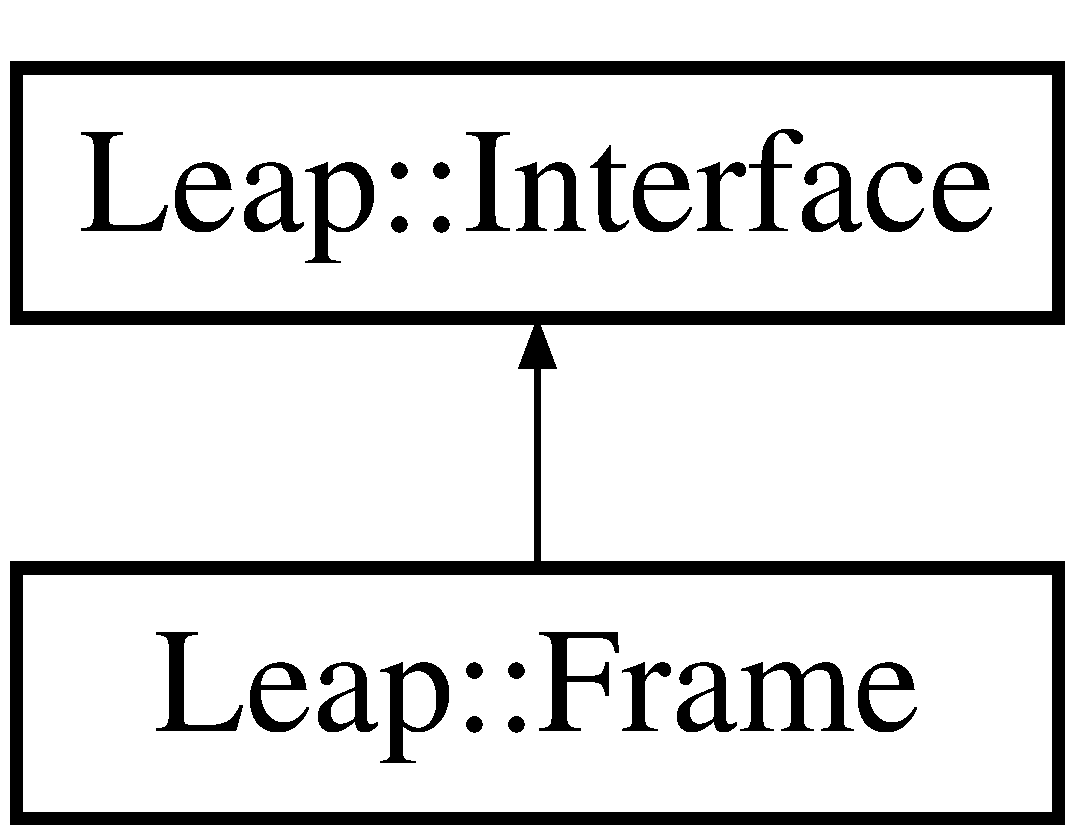
\includegraphics[height=2.000000cm]{class_leap_1_1_frame}
\end{center}
\end{figure}
\subsection*{Public Member Functions}
\begin{DoxyCompactItemize}
\item 
\hypertarget{class_leap_1_1_frame_a95352396f81805bde0b3e1bb76960519}{{\bfseries Frame} (Frame\+Implementation $\ast$)}\label{class_leap_1_1_frame_a95352396f81805bde0b3e1bb76960519}

\item 
L\+E\+A\+P\+\_\+\+E\+X\+P\+O\+R\+T \hyperlink{class_leap_1_1_frame_a6a619578cc80bcdf65f9f332a2432a2f}{Frame} ()
\item 
L\+E\+A\+P\+\_\+\+E\+X\+P\+O\+R\+T int64\+\_\+t \hyperlink{class_leap_1_1_frame_aaa0ab37b441f635a293f577dc9b2d20f}{id} () const 
\item 
L\+E\+A\+P\+\_\+\+E\+X\+P\+O\+R\+T int64\+\_\+t \hyperlink{class_leap_1_1_frame_a631c8c5e5490ee07e7823a62e432dfea}{timestamp} () const 
\item 
L\+E\+A\+P\+\_\+\+E\+X\+P\+O\+R\+T \hyperlink{class_leap_1_1_hand_list}{Hand\+List} \hyperlink{class_leap_1_1_frame_ab9e46956b8a90dafdce75803b4b6bdf8}{hands} () const 
\item 
L\+E\+A\+P\+\_\+\+E\+X\+P\+O\+R\+T \hyperlink{class_leap_1_1_hand}{Hand} \hyperlink{class_leap_1_1_frame_a7565082f9b3cdaf12b620c2e1d278912}{hand} (int32\+\_\+t \hyperlink{class_leap_1_1_frame_aaa0ab37b441f635a293f577dc9b2d20f}{id}) const 
\item 
L\+E\+A\+P\+\_\+\+E\+X\+P\+O\+R\+T \hyperlink{class_leap_1_1_pointable_list}{Pointable\+List} \hyperlink{class_leap_1_1_frame_a1bc989343a3b971568368c77b5869fb9}{pointables} () const 
\item 
L\+E\+A\+P\+\_\+\+E\+X\+P\+O\+R\+T \hyperlink{class_leap_1_1_pointable}{Pointable} \hyperlink{class_leap_1_1_frame_a965d1e23e9ad84420359711768ff1fab}{pointable} (int32\+\_\+t \hyperlink{class_leap_1_1_frame_aaa0ab37b441f635a293f577dc9b2d20f}{id}) const 
\item 
L\+E\+A\+P\+\_\+\+E\+X\+P\+O\+R\+T \hyperlink{class_leap_1_1_finger_list}{Finger\+List} \hyperlink{class_leap_1_1_frame_abff33c86515d42793abf134e359e5142}{fingers} () const 
\item 
L\+E\+A\+P\+\_\+\+E\+X\+P\+O\+R\+T \hyperlink{class_leap_1_1_finger}{Finger} \hyperlink{class_leap_1_1_frame_a2f146a5c9103c9708dc4d120d18f6c40}{finger} (int32\+\_\+t \hyperlink{class_leap_1_1_frame_aaa0ab37b441f635a293f577dc9b2d20f}{id}) const 
\item 
L\+E\+A\+P\+\_\+\+E\+X\+P\+O\+R\+T \hyperlink{class_leap_1_1_tool_list}{Tool\+List} \hyperlink{class_leap_1_1_frame_abf81ff857abdd1cc9c2ccb889eb1c6e3}{tools} () const 
\item 
L\+E\+A\+P\+\_\+\+E\+X\+P\+O\+R\+T \hyperlink{class_leap_1_1_tool}{Tool} \hyperlink{class_leap_1_1_frame_aa12947e61dbbf470d4ee4906c7928f08}{tool} (int32\+\_\+t \hyperlink{class_leap_1_1_frame_aaa0ab37b441f635a293f577dc9b2d20f}{id}) const 
\item 
L\+E\+A\+P\+\_\+\+E\+X\+P\+O\+R\+T \hyperlink{class_leap_1_1_gesture}{Gesture} \hyperlink{class_leap_1_1_frame_afb0577b99e3bc259c4e20a710062c926}{gesture} (int32\+\_\+t \hyperlink{class_leap_1_1_frame_aaa0ab37b441f635a293f577dc9b2d20f}{id}) const 
\item 
L\+E\+A\+P\+\_\+\+E\+X\+P\+O\+R\+T \hyperlink{class_leap_1_1_gesture_list}{Gesture\+List} \hyperlink{class_leap_1_1_frame_a4e4dfb7dbe7796d836fdbec255909379}{gestures} () const 
\item 
L\+E\+A\+P\+\_\+\+E\+X\+P\+O\+R\+T \hyperlink{class_leap_1_1_gesture_list}{Gesture\+List} \hyperlink{class_leap_1_1_frame_a5e85715286974e35d5ea557da19aafbb}{gestures} (const \hyperlink{class_leap_1_1_frame}{Frame} \&since\+Frame) const 
\item 
L\+E\+A\+P\+\_\+\+E\+X\+P\+O\+R\+T \hyperlink{struct_leap_1_1_vector}{Vector} \hyperlink{class_leap_1_1_frame_a086cdc5e4d525590c553c2c250e04458}{translation} (const \hyperlink{class_leap_1_1_frame}{Frame} \&since\+Frame) const 
\item 
L\+E\+A\+P\+\_\+\+E\+X\+P\+O\+R\+T float \hyperlink{class_leap_1_1_frame_a2aa8c89a3d9a16fa6a674e95ecd9e31f}{translation\+Probability} (const \hyperlink{class_leap_1_1_frame}{Frame} \&since\+Frame) const 
\item 
L\+E\+A\+P\+\_\+\+E\+X\+P\+O\+R\+T \hyperlink{struct_leap_1_1_vector}{Vector} \hyperlink{class_leap_1_1_frame_a40411646c821ded2c1a1604d63ccba29}{rotation\+Axis} (const \hyperlink{class_leap_1_1_frame}{Frame} \&since\+Frame) const 
\item 
L\+E\+A\+P\+\_\+\+E\+X\+P\+O\+R\+T float \hyperlink{class_leap_1_1_frame_ac7ea6b9924b093854a5aef00b5f4ec94}{rotation\+Angle} (const \hyperlink{class_leap_1_1_frame}{Frame} \&since\+Frame) const 
\item 
L\+E\+A\+P\+\_\+\+E\+X\+P\+O\+R\+T float \hyperlink{class_leap_1_1_frame_a0a280ad7f99d52ee08c4ae99362fce62}{rotation\+Angle} (const \hyperlink{class_leap_1_1_frame}{Frame} \&since\+Frame, const \hyperlink{struct_leap_1_1_vector}{Vector} \&axis) const 
\item 
L\+E\+A\+P\+\_\+\+E\+X\+P\+O\+R\+T \hyperlink{struct_leap_1_1_matrix}{Matrix} \hyperlink{class_leap_1_1_frame_a06fcbc22654ef3a06e657f6b55d94aaf}{rotation\+Matrix} (const \hyperlink{class_leap_1_1_frame}{Frame} \&since\+Frame) const 
\item 
L\+E\+A\+P\+\_\+\+E\+X\+P\+O\+R\+T float \hyperlink{class_leap_1_1_frame_a8005272f410431448620af1269ae0127}{rotation\+Probability} (const \hyperlink{class_leap_1_1_frame}{Frame} \&since\+Frame) const 
\item 
L\+E\+A\+P\+\_\+\+E\+X\+P\+O\+R\+T float \hyperlink{class_leap_1_1_frame_a8786d67154ab10f0b36f2b39c1e1541d}{scale\+Factor} (const \hyperlink{class_leap_1_1_frame}{Frame} \&since\+Frame) const 
\item 
L\+E\+A\+P\+\_\+\+E\+X\+P\+O\+R\+T float \hyperlink{class_leap_1_1_frame_addf9f652ce205b8a827fb3fe18345e36}{scale\+Probability} (const \hyperlink{class_leap_1_1_frame}{Frame} \&since\+Frame) const 
\item 
L\+E\+A\+P\+\_\+\+E\+X\+P\+O\+R\+T \hyperlink{class_leap_1_1_interaction_box}{Interaction\+Box} \hyperlink{class_leap_1_1_frame_abe8b9f619d30dec76b5cd5bfcabddf98}{interaction\+Box} () const 
\item 
L\+E\+A\+P\+\_\+\+E\+X\+P\+O\+R\+T float \hyperlink{class_leap_1_1_frame_a9a881e9c40c667c47c029a803fa2afa6}{current\+Frames\+Per\+Second} () const 
\item 
L\+E\+A\+P\+\_\+\+E\+X\+P\+O\+R\+T bool \hyperlink{class_leap_1_1_frame_ab5dc8d5562c21a65885999fda4d52a8f}{is\+Valid} () const 
\item 
L\+E\+A\+P\+\_\+\+E\+X\+P\+O\+R\+T bool \hyperlink{class_leap_1_1_frame_a6d26f359703ee46db2e50d3eb86e868a}{operator==} (const \hyperlink{class_leap_1_1_frame}{Frame} \&) const 
\item 
L\+E\+A\+P\+\_\+\+E\+X\+P\+O\+R\+T bool \hyperlink{class_leap_1_1_frame_ad8558771021e0904a9933cfedb491639}{operator!=} (const \hyperlink{class_leap_1_1_frame}{Frame} \&) const 
\item 
L\+E\+A\+P\+\_\+\+E\+X\+P\+O\+R\+T std\+::string \hyperlink{class_leap_1_1_frame_a94ec0c7a340f813d6e357d83891cf8e1}{to\+String} () const 
\end{DoxyCompactItemize}
\subsection*{Static Public Member Functions}
\begin{DoxyCompactItemize}
\item 
static L\+E\+A\+P\+\_\+\+E\+X\+P\+O\+R\+T const \hyperlink{class_leap_1_1_frame}{Frame} \& \hyperlink{class_leap_1_1_frame_a069854a98be43ae91a9f23058674d2eb}{invalid} ()
\end{DoxyCompactItemize}
\subsection*{Friends}
\begin{DoxyCompactItemize}
\item 
L\+E\+A\+P\+\_\+\+E\+X\+P\+O\+R\+T friend std\+::ostream \& \hyperlink{class_leap_1_1_frame_a3eb142cc11b68e23a4aaa42c7784c6d2}{operator$<$$<$} (std\+::ostream \&, const \hyperlink{class_leap_1_1_frame}{Frame} \&)
\end{DoxyCompactItemize}
\subsection*{Additional Inherited Members}


\subsection{Detailed Description}
The \hyperlink{class_leap_1_1_frame}{Frame} class represents a set of hand and finger tracking data detected in a single frame.

The Leap Motion software detects hands, fingers and tools within the tracking area, reporting their positions, orientations and motions in frames at the Leap Motion frame rate.

Access \hyperlink{class_leap_1_1_frame}{Frame} objects through an instance of the \hyperlink{class_leap_1_1_controller}{Controller} class. Implement a \hyperlink{class_leap_1_1_listener}{Listener} subclass to receive a callback event when a new \hyperlink{class_leap_1_1_frame}{Frame} is available. \begin{DoxySince}{Since}
1.\+0 
\end{DoxySince}


\subsection{Constructor \& Destructor Documentation}
\hypertarget{class_leap_1_1_frame_a6a619578cc80bcdf65f9f332a2432a2f}{\index{Leap\+::\+Frame@{Leap\+::\+Frame}!Frame@{Frame}}
\index{Frame@{Frame}!Leap\+::\+Frame@{Leap\+::\+Frame}}
\subsubsection[{Frame}]{\setlength{\rightskip}{0pt plus 5cm}L\+E\+A\+P\+\_\+\+E\+X\+P\+O\+R\+T Leap\+::\+Frame\+::\+Frame (
\begin{DoxyParamCaption}
{}
\end{DoxyParamCaption}
)}}\label{class_leap_1_1_frame_a6a619578cc80bcdf65f9f332a2432a2f}
Constructs a \hyperlink{class_leap_1_1_frame}{Frame} object.

\hyperlink{class_leap_1_1_frame}{Frame} instances created with this constructor are invalid. Get valid \hyperlink{class_leap_1_1_frame}{Frame} objects by calling the \hyperlink{class_leap_1_1_controller_a5796b988806ea9fd94e2d987e0e24b32}{Controller\+::frame()} function. \begin{DoxySince}{Since}
1.\+0 
\end{DoxySince}


\subsection{Member Function Documentation}
\hypertarget{class_leap_1_1_frame_a9a881e9c40c667c47c029a803fa2afa6}{\index{Leap\+::\+Frame@{Leap\+::\+Frame}!current\+Frames\+Per\+Second@{current\+Frames\+Per\+Second}}
\index{current\+Frames\+Per\+Second@{current\+Frames\+Per\+Second}!Leap\+::\+Frame@{Leap\+::\+Frame}}
\subsubsection[{current\+Frames\+Per\+Second}]{\setlength{\rightskip}{0pt plus 5cm}L\+E\+A\+P\+\_\+\+E\+X\+P\+O\+R\+T float Leap\+::\+Frame\+::current\+Frames\+Per\+Second (
\begin{DoxyParamCaption}
{}
\end{DoxyParamCaption}
) const}}\label{class_leap_1_1_frame_a9a881e9c40c667c47c029a803fa2afa6}
The instantaneous framerate.

The rate at which the Leap Motion software is providing frames of data (in frames per second). The framerate can fluctuate depending on available computing resources, activity within the device field of view, software tracking settings, and other factors.

\begin{DoxyReturn}{Returns}
An estimate of frames per second of the Leap Motion \hyperlink{class_leap_1_1_controller}{Controller}. 
\end{DoxyReturn}
\begin{DoxySince}{Since}
1.\+0 
\end{DoxySince}
\hypertarget{class_leap_1_1_frame_a2f146a5c9103c9708dc4d120d18f6c40}{\index{Leap\+::\+Frame@{Leap\+::\+Frame}!finger@{finger}}
\index{finger@{finger}!Leap\+::\+Frame@{Leap\+::\+Frame}}
\subsubsection[{finger}]{\setlength{\rightskip}{0pt plus 5cm}L\+E\+A\+P\+\_\+\+E\+X\+P\+O\+R\+T {\bf Finger} Leap\+::\+Frame\+::finger (
\begin{DoxyParamCaption}
\item[{int32\+\_\+t}]{id}
\end{DoxyParamCaption}
) const}}\label{class_leap_1_1_frame_a2f146a5c9103c9708dc4d120d18f6c40}
The \hyperlink{class_leap_1_1_finger}{Finger} object with the specified I\+D in this frame.

Use the \hyperlink{class_leap_1_1_frame_a2f146a5c9103c9708dc4d120d18f6c40}{Frame\+::finger()} function to retrieve the \hyperlink{class_leap_1_1_finger}{Finger} object from this frame using an I\+D value obtained from a previous frame. This function always returns a \hyperlink{class_leap_1_1_finger}{Finger} object, but if no finger with the specified I\+D is present, an invalid \hyperlink{class_leap_1_1_finger}{Finger} object is returned.

Note that I\+D values persist across frames, but only until tracking of a particular object is lost. If tracking of a finger is lost and subsequently regained, the new \hyperlink{class_leap_1_1_finger}{Finger} object representing that physical finger may have a different I\+D than that representing the finger in an earlier frame.


\begin{DoxyParams}{Parameters}
{\em id} & The I\+D value of a \hyperlink{class_leap_1_1_finger}{Finger} object from a previous frame. \\
\hline
\end{DoxyParams}
\begin{DoxyReturn}{Returns}
The \hyperlink{class_leap_1_1_finger}{Finger} object with the matching I\+D if one exists in this frame; otherwise, an invalid \hyperlink{class_leap_1_1_finger}{Finger} object is returned. 
\end{DoxyReturn}
\begin{DoxySince}{Since}
1.\+0 
\end{DoxySince}
\hypertarget{class_leap_1_1_frame_abff33c86515d42793abf134e359e5142}{\index{Leap\+::\+Frame@{Leap\+::\+Frame}!fingers@{fingers}}
\index{fingers@{fingers}!Leap\+::\+Frame@{Leap\+::\+Frame}}
\subsubsection[{fingers}]{\setlength{\rightskip}{0pt plus 5cm}L\+E\+A\+P\+\_\+\+E\+X\+P\+O\+R\+T {\bf Finger\+List} Leap\+::\+Frame\+::fingers (
\begin{DoxyParamCaption}
{}
\end{DoxyParamCaption}
) const}}\label{class_leap_1_1_frame_abff33c86515d42793abf134e359e5142}
The list of \hyperlink{class_leap_1_1_finger}{Finger} objects detected in this frame, given in arbitrary order. The list can be empty if no fingers are detected.

\begin{DoxyReturn}{Returns}
The \hyperlink{class_leap_1_1_finger_list}{Finger\+List} containing all \hyperlink{class_leap_1_1_finger}{Finger} objects detected in this frame. 
\end{DoxyReturn}
\begin{DoxySince}{Since}
1.\+0 
\end{DoxySince}
\hypertarget{class_leap_1_1_frame_afb0577b99e3bc259c4e20a710062c926}{\index{Leap\+::\+Frame@{Leap\+::\+Frame}!gesture@{gesture}}
\index{gesture@{gesture}!Leap\+::\+Frame@{Leap\+::\+Frame}}
\subsubsection[{gesture}]{\setlength{\rightskip}{0pt plus 5cm}L\+E\+A\+P\+\_\+\+E\+X\+P\+O\+R\+T {\bf Gesture} Leap\+::\+Frame\+::gesture (
\begin{DoxyParamCaption}
\item[{int32\+\_\+t}]{id}
\end{DoxyParamCaption}
) const}}\label{class_leap_1_1_frame_afb0577b99e3bc259c4e20a710062c926}
The \hyperlink{class_leap_1_1_gesture}{Gesture} object with the specified I\+D in this frame.

Use the \hyperlink{class_leap_1_1_frame_afb0577b99e3bc259c4e20a710062c926}{Frame\+::gesture()} function to return a \hyperlink{class_leap_1_1_gesture}{Gesture} object in this frame using an I\+D obtained in an earlier frame. The function always returns a \hyperlink{class_leap_1_1_gesture}{Gesture} object, but if there was no update for the gesture in this frame, then an invalid \hyperlink{class_leap_1_1_gesture}{Gesture} object is returned.

All \hyperlink{class_leap_1_1_gesture}{Gesture} objects representing the same recognized movement share the same I\+D. 
\begin{DoxyParams}{Parameters}
{\em id} & The I\+D of an \hyperlink{class_leap_1_1_gesture}{Gesture} object from a previous frame. \\
\hline
\end{DoxyParams}
\begin{DoxyReturn}{Returns}
The \hyperlink{class_leap_1_1_gesture}{Gesture} object in the frame with the specified I\+D if one exists; Otherwise, an Invalid \hyperlink{class_leap_1_1_gesture}{Gesture} object. 
\end{DoxyReturn}
\begin{DoxySince}{Since}
1.\+0 
\end{DoxySince}
\hypertarget{class_leap_1_1_frame_a4e4dfb7dbe7796d836fdbec255909379}{\index{Leap\+::\+Frame@{Leap\+::\+Frame}!gestures@{gestures}}
\index{gestures@{gestures}!Leap\+::\+Frame@{Leap\+::\+Frame}}
\subsubsection[{gestures}]{\setlength{\rightskip}{0pt plus 5cm}L\+E\+A\+P\+\_\+\+E\+X\+P\+O\+R\+T {\bf Gesture\+List} Leap\+::\+Frame\+::gestures (
\begin{DoxyParamCaption}
{}
\end{DoxyParamCaption}
) const}}\label{class_leap_1_1_frame_a4e4dfb7dbe7796d836fdbec255909379}
The gestures recognized or continuing in this frame.

Circle and swipe gestures are updated every frame. Tap gestures only appear in the list for a single frame.

\begin{DoxyReturn}{Returns}
\hyperlink{class_leap_1_1_gesture_list}{Gesture\+List} the list of gestures. 
\end{DoxyReturn}
\begin{DoxySince}{Since}
1.\+0 
\end{DoxySince}
\hypertarget{class_leap_1_1_frame_a5e85715286974e35d5ea557da19aafbb}{\index{Leap\+::\+Frame@{Leap\+::\+Frame}!gestures@{gestures}}
\index{gestures@{gestures}!Leap\+::\+Frame@{Leap\+::\+Frame}}
\subsubsection[{gestures}]{\setlength{\rightskip}{0pt plus 5cm}L\+E\+A\+P\+\_\+\+E\+X\+P\+O\+R\+T {\bf Gesture\+List} Leap\+::\+Frame\+::gestures (
\begin{DoxyParamCaption}
\item[{const {\bf Frame} \&}]{since\+Frame}
\end{DoxyParamCaption}
) const}}\label{class_leap_1_1_frame_a5e85715286974e35d5ea557da19aafbb}
Returns a \hyperlink{class_leap_1_1_gesture_list}{Gesture\+List} containing all gestures that have occured since the specified frame.


\begin{DoxyParams}{Parameters}
{\em since\+Frame} & An earlier \hyperlink{class_leap_1_1_frame}{Frame} object. The starting frame must still be in the frame history cache, which has a default length of 60 frames. \\
\hline
\end{DoxyParams}
\begin{DoxyReturn}{Returns}
\hyperlink{class_leap_1_1_gesture_list}{Gesture\+List} The list of the \hyperlink{class_leap_1_1_gesture}{Gesture} objects that have occured since the specified frame. 
\end{DoxyReturn}
\begin{DoxySince}{Since}
1.\+0 
\end{DoxySince}
\hypertarget{class_leap_1_1_frame_a7565082f9b3cdaf12b620c2e1d278912}{\index{Leap\+::\+Frame@{Leap\+::\+Frame}!hand@{hand}}
\index{hand@{hand}!Leap\+::\+Frame@{Leap\+::\+Frame}}
\subsubsection[{hand}]{\setlength{\rightskip}{0pt plus 5cm}L\+E\+A\+P\+\_\+\+E\+X\+P\+O\+R\+T {\bf Hand} Leap\+::\+Frame\+::hand (
\begin{DoxyParamCaption}
\item[{int32\+\_\+t}]{id}
\end{DoxyParamCaption}
) const}}\label{class_leap_1_1_frame_a7565082f9b3cdaf12b620c2e1d278912}
The \hyperlink{class_leap_1_1_hand}{Hand} object with the specified I\+D in this frame.

Use the \hyperlink{class_leap_1_1_frame_a7565082f9b3cdaf12b620c2e1d278912}{Frame\+::hand()} function to retrieve the \hyperlink{class_leap_1_1_hand}{Hand} object from this frame using an I\+D value obtained from a previous frame. This function always returns a \hyperlink{class_leap_1_1_hand}{Hand} object, but if no hand with the specified I\+D is present, an invalid \hyperlink{class_leap_1_1_hand}{Hand} object is returned.

Note that I\+D values persist across frames, but only until tracking of a particular object is lost. If tracking of a hand is lost and subsequently regained, the new \hyperlink{class_leap_1_1_hand}{Hand} object representing that physical hand may have a different I\+D than that representing the physical hand in an earlier frame.


\begin{DoxyParams}{Parameters}
{\em id} & The I\+D value of a \hyperlink{class_leap_1_1_hand}{Hand} object from a previous frame. \\
\hline
\end{DoxyParams}
\begin{DoxyReturn}{Returns}
The \hyperlink{class_leap_1_1_hand}{Hand} object with the matching I\+D if one exists in this frame; otherwise, an invalid \hyperlink{class_leap_1_1_hand}{Hand} object is returned. 
\end{DoxyReturn}
\begin{DoxySince}{Since}
1.\+0 
\end{DoxySince}
\hypertarget{class_leap_1_1_frame_ab9e46956b8a90dafdce75803b4b6bdf8}{\index{Leap\+::\+Frame@{Leap\+::\+Frame}!hands@{hands}}
\index{hands@{hands}!Leap\+::\+Frame@{Leap\+::\+Frame}}
\subsubsection[{hands}]{\setlength{\rightskip}{0pt plus 5cm}L\+E\+A\+P\+\_\+\+E\+X\+P\+O\+R\+T {\bf Hand\+List} Leap\+::\+Frame\+::hands (
\begin{DoxyParamCaption}
{}
\end{DoxyParamCaption}
) const}}\label{class_leap_1_1_frame_ab9e46956b8a90dafdce75803b4b6bdf8}
The list of \hyperlink{class_leap_1_1_hand}{Hand} objects detected in this frame, given in arbitrary order. The list can be empty if no hands are detected.

\begin{DoxyReturn}{Returns}
The \hyperlink{class_leap_1_1_hand_list}{Hand\+List} containing all \hyperlink{class_leap_1_1_hand}{Hand} objects detected in this frame. 
\end{DoxyReturn}
\begin{DoxySince}{Since}
1.\+0 
\end{DoxySince}
\hypertarget{class_leap_1_1_frame_aaa0ab37b441f635a293f577dc9b2d20f}{\index{Leap\+::\+Frame@{Leap\+::\+Frame}!id@{id}}
\index{id@{id}!Leap\+::\+Frame@{Leap\+::\+Frame}}
\subsubsection[{id}]{\setlength{\rightskip}{0pt plus 5cm}L\+E\+A\+P\+\_\+\+E\+X\+P\+O\+R\+T int64\+\_\+t Leap\+::\+Frame\+::id (
\begin{DoxyParamCaption}
{}
\end{DoxyParamCaption}
) const}}\label{class_leap_1_1_frame_aaa0ab37b441f635a293f577dc9b2d20f}
A unique I\+D for this \hyperlink{class_leap_1_1_frame}{Frame}. Consecutive frames processed by the Leap Motion software have consecutive increasing values.

\begin{DoxyReturn}{Returns}
The frame I\+D. 
\end{DoxyReturn}
\begin{DoxySince}{Since}
1.\+0 
\end{DoxySince}
\hypertarget{class_leap_1_1_frame_abe8b9f619d30dec76b5cd5bfcabddf98}{\index{Leap\+::\+Frame@{Leap\+::\+Frame}!interaction\+Box@{interaction\+Box}}
\index{interaction\+Box@{interaction\+Box}!Leap\+::\+Frame@{Leap\+::\+Frame}}
\subsubsection[{interaction\+Box}]{\setlength{\rightskip}{0pt plus 5cm}L\+E\+A\+P\+\_\+\+E\+X\+P\+O\+R\+T {\bf Interaction\+Box} Leap\+::\+Frame\+::interaction\+Box (
\begin{DoxyParamCaption}
{}
\end{DoxyParamCaption}
) const}}\label{class_leap_1_1_frame_abe8b9f619d30dec76b5cd5bfcabddf98}
The current \hyperlink{class_leap_1_1_interaction_box}{Interaction\+Box} for the frame. See the \hyperlink{class_leap_1_1_interaction_box}{Interaction\+Box} class documentation for more details on how this class should be used.

\begin{DoxyReturn}{Returns}
The current \hyperlink{class_leap_1_1_interaction_box}{Interaction\+Box} object. 
\end{DoxyReturn}
\begin{DoxySince}{Since}
1.\+0 
\end{DoxySince}
\hypertarget{class_leap_1_1_frame_a069854a98be43ae91a9f23058674d2eb}{\index{Leap\+::\+Frame@{Leap\+::\+Frame}!invalid@{invalid}}
\index{invalid@{invalid}!Leap\+::\+Frame@{Leap\+::\+Frame}}
\subsubsection[{invalid}]{\setlength{\rightskip}{0pt plus 5cm}static L\+E\+A\+P\+\_\+\+E\+X\+P\+O\+R\+T const {\bf Frame}\& Leap\+::\+Frame\+::invalid (
\begin{DoxyParamCaption}
{}
\end{DoxyParamCaption}
)\hspace{0.3cm}{\ttfamily [static]}}}\label{class_leap_1_1_frame_a069854a98be43ae91a9f23058674d2eb}
Returns an invalid \hyperlink{class_leap_1_1_frame}{Frame} object.

You can use the instance returned by this function in comparisons testing whether a given \hyperlink{class_leap_1_1_frame}{Frame} instance is valid or invalid. (You can also use the \hyperlink{class_leap_1_1_frame_ab5dc8d5562c21a65885999fda4d52a8f}{Frame\+::is\+Valid()} function.)

\begin{DoxyReturn}{Returns}
The invalid \hyperlink{class_leap_1_1_frame}{Frame} instance. 
\end{DoxyReturn}
\begin{DoxySince}{Since}
1.\+0 
\end{DoxySince}
\hypertarget{class_leap_1_1_frame_ab5dc8d5562c21a65885999fda4d52a8f}{\index{Leap\+::\+Frame@{Leap\+::\+Frame}!is\+Valid@{is\+Valid}}
\index{is\+Valid@{is\+Valid}!Leap\+::\+Frame@{Leap\+::\+Frame}}
\subsubsection[{is\+Valid}]{\setlength{\rightskip}{0pt plus 5cm}L\+E\+A\+P\+\_\+\+E\+X\+P\+O\+R\+T bool Leap\+::\+Frame\+::is\+Valid (
\begin{DoxyParamCaption}
{}
\end{DoxyParamCaption}
) const}}\label{class_leap_1_1_frame_ab5dc8d5562c21a65885999fda4d52a8f}
Reports whether this \hyperlink{class_leap_1_1_frame}{Frame} instance is valid.

A valid \hyperlink{class_leap_1_1_frame}{Frame} is one generated by the \hyperlink{class_leap_1_1_controller}{Leap\+::\+Controller} object that contains tracking data for all detected entities. An invalid \hyperlink{class_leap_1_1_frame}{Frame} contains no actual tracking data, but you can call its functions without risk of a null pointer exception. The invalid \hyperlink{class_leap_1_1_frame}{Frame} mechanism makes it more convenient to track individual data across the frame history. For example, you can invoke\+:


\begin{DoxyCodeInclude}
\end{DoxyCodeInclude}


for an arbitrary \hyperlink{class_leap_1_1_frame}{Frame} history value, \char`\"{}n\char`\"{}, without first checking whether frame(n) returned a null object. (You should still check that the returned \hyperlink{class_leap_1_1_finger}{Finger} instance is valid.)

\begin{DoxyReturn}{Returns}
True, if this is a valid \hyperlink{class_leap_1_1_frame}{Frame} object; false otherwise. 
\end{DoxyReturn}
\begin{DoxySince}{Since}
1.\+0 
\end{DoxySince}
\hypertarget{class_leap_1_1_frame_ad8558771021e0904a9933cfedb491639}{\index{Leap\+::\+Frame@{Leap\+::\+Frame}!operator"!=@{operator"!=}}
\index{operator"!=@{operator"!=}!Leap\+::\+Frame@{Leap\+::\+Frame}}
\subsubsection[{operator"!=}]{\setlength{\rightskip}{0pt plus 5cm}L\+E\+A\+P\+\_\+\+E\+X\+P\+O\+R\+T bool Leap\+::\+Frame\+::operator!= (
\begin{DoxyParamCaption}
\item[{const {\bf Frame} \&}]{}
\end{DoxyParamCaption}
) const}}\label{class_leap_1_1_frame_ad8558771021e0904a9933cfedb491639}
Compare \hyperlink{class_leap_1_1_frame}{Frame} object inequality. Two \hyperlink{class_leap_1_1_frame}{Frame} objects are equal if and only if both \hyperlink{class_leap_1_1_frame}{Frame} objects represent the exact same frame of tracking data and both \hyperlink{class_leap_1_1_frame}{Frame} objects are valid. \begin{DoxySince}{Since}
1.\+0 
\end{DoxySince}
\hypertarget{class_leap_1_1_frame_a6d26f359703ee46db2e50d3eb86e868a}{\index{Leap\+::\+Frame@{Leap\+::\+Frame}!operator==@{operator==}}
\index{operator==@{operator==}!Leap\+::\+Frame@{Leap\+::\+Frame}}
\subsubsection[{operator==}]{\setlength{\rightskip}{0pt plus 5cm}L\+E\+A\+P\+\_\+\+E\+X\+P\+O\+R\+T bool Leap\+::\+Frame\+::operator== (
\begin{DoxyParamCaption}
\item[{const {\bf Frame} \&}]{}
\end{DoxyParamCaption}
) const}}\label{class_leap_1_1_frame_a6d26f359703ee46db2e50d3eb86e868a}
Compare \hyperlink{class_leap_1_1_frame}{Frame} object equality. Two \hyperlink{class_leap_1_1_frame}{Frame} objects are equal if and only if both \hyperlink{class_leap_1_1_frame}{Frame} objects represent the exact same frame of tracking data and both \hyperlink{class_leap_1_1_frame}{Frame} objects are valid. \begin{DoxySince}{Since}
1.\+0 
\end{DoxySince}
\hypertarget{class_leap_1_1_frame_a965d1e23e9ad84420359711768ff1fab}{\index{Leap\+::\+Frame@{Leap\+::\+Frame}!pointable@{pointable}}
\index{pointable@{pointable}!Leap\+::\+Frame@{Leap\+::\+Frame}}
\subsubsection[{pointable}]{\setlength{\rightskip}{0pt plus 5cm}L\+E\+A\+P\+\_\+\+E\+X\+P\+O\+R\+T {\bf Pointable} Leap\+::\+Frame\+::pointable (
\begin{DoxyParamCaption}
\item[{int32\+\_\+t}]{id}
\end{DoxyParamCaption}
) const}}\label{class_leap_1_1_frame_a965d1e23e9ad84420359711768ff1fab}
The \hyperlink{class_leap_1_1_pointable}{Pointable} object with the specified I\+D in this frame.

Use the \hyperlink{class_leap_1_1_frame_a965d1e23e9ad84420359711768ff1fab}{Frame\+::pointable()} function to retrieve the \hyperlink{class_leap_1_1_pointable}{Pointable} object from this frame using an I\+D value obtained from a previous frame. This function always returns a \hyperlink{class_leap_1_1_pointable}{Pointable} object, but if no finger or tool with the specified I\+D is present, an invalid \hyperlink{class_leap_1_1_pointable}{Pointable} object is returned.

Note that I\+D values persist across frames, but only until tracking of a particular object is lost. If tracking of a finger or tool is lost and subsequently regained, the new \hyperlink{class_leap_1_1_pointable}{Pointable} object representing that finger or tool may have a different I\+D than that representing the finger or tool in an earlier frame.


\begin{DoxyParams}{Parameters}
{\em id} & The I\+D value of a \hyperlink{class_leap_1_1_pointable}{Pointable} object from a previous frame. \\
\hline
\end{DoxyParams}
\begin{DoxyReturn}{Returns}
The \hyperlink{class_leap_1_1_pointable}{Pointable} object with the matching I\+D if one exists in this frame; otherwise, an invalid \hyperlink{class_leap_1_1_pointable}{Pointable} object is returned. 
\end{DoxyReturn}
\begin{DoxySince}{Since}
1.\+0 
\end{DoxySince}
\hypertarget{class_leap_1_1_frame_a1bc989343a3b971568368c77b5869fb9}{\index{Leap\+::\+Frame@{Leap\+::\+Frame}!pointables@{pointables}}
\index{pointables@{pointables}!Leap\+::\+Frame@{Leap\+::\+Frame}}
\subsubsection[{pointables}]{\setlength{\rightskip}{0pt plus 5cm}L\+E\+A\+P\+\_\+\+E\+X\+P\+O\+R\+T {\bf Pointable\+List} Leap\+::\+Frame\+::pointables (
\begin{DoxyParamCaption}
{}
\end{DoxyParamCaption}
) const}}\label{class_leap_1_1_frame_a1bc989343a3b971568368c77b5869fb9}
The list of \hyperlink{class_leap_1_1_pointable}{Pointable} objects (fingers and tools) detected in this frame, given in arbitrary order. The list can be empty if no fingers or tools are detected.

\begin{DoxyReturn}{Returns}
The \hyperlink{class_leap_1_1_pointable_list}{Pointable\+List} containing all \hyperlink{class_leap_1_1_pointable}{Pointable} objects detected in this frame. 
\end{DoxyReturn}
\begin{DoxySince}{Since}
1.\+0 
\end{DoxySince}
\hypertarget{class_leap_1_1_frame_ac7ea6b9924b093854a5aef00b5f4ec94}{\index{Leap\+::\+Frame@{Leap\+::\+Frame}!rotation\+Angle@{rotation\+Angle}}
\index{rotation\+Angle@{rotation\+Angle}!Leap\+::\+Frame@{Leap\+::\+Frame}}
\subsubsection[{rotation\+Angle}]{\setlength{\rightskip}{0pt plus 5cm}L\+E\+A\+P\+\_\+\+E\+X\+P\+O\+R\+T float Leap\+::\+Frame\+::rotation\+Angle (
\begin{DoxyParamCaption}
\item[{const {\bf Frame} \&}]{since\+Frame}
\end{DoxyParamCaption}
) const}}\label{class_leap_1_1_frame_ac7ea6b9924b093854a5aef00b5f4ec94}
The angle of rotation around the rotation axis derived from the overall rotational motion between the current frame and the specified frame.

The returned angle is expressed in radians measured clockwise around the rotation axis (using the right-\/hand rule) between the start and end frames. The value is always between 0 and pi radians (0 and 180 degrees).

The Leap Motion software derives frame rotation from the relative change in position and orientation of all objects detected in the field of view.

If either this frame or since\+Frame is an invalid \hyperlink{class_leap_1_1_frame}{Frame} object, then the angle of rotation is zero.


\begin{DoxyParams}{Parameters}
{\em since\+Frame} & The starting frame for computing the relative rotation. \\
\hline
\end{DoxyParams}
\begin{DoxyReturn}{Returns}
A positive value containing the heuristically determined rotational change between the current frame and that specified in the since\+Frame parameter. 
\end{DoxyReturn}
\begin{DoxySince}{Since}
1.\+0 
\end{DoxySince}
\hypertarget{class_leap_1_1_frame_a0a280ad7f99d52ee08c4ae99362fce62}{\index{Leap\+::\+Frame@{Leap\+::\+Frame}!rotation\+Angle@{rotation\+Angle}}
\index{rotation\+Angle@{rotation\+Angle}!Leap\+::\+Frame@{Leap\+::\+Frame}}
\subsubsection[{rotation\+Angle}]{\setlength{\rightskip}{0pt plus 5cm}L\+E\+A\+P\+\_\+\+E\+X\+P\+O\+R\+T float Leap\+::\+Frame\+::rotation\+Angle (
\begin{DoxyParamCaption}
\item[{const {\bf Frame} \&}]{since\+Frame, }
\item[{const {\bf Vector} \&}]{axis}
\end{DoxyParamCaption}
) const}}\label{class_leap_1_1_frame_a0a280ad7f99d52ee08c4ae99362fce62}
The angle of rotation around the specified axis derived from the overall rotational motion between the current frame and the specified frame.

The returned angle is expressed in radians measured clockwise around the rotation axis (using the right-\/hand rule) between the start and end frames. The value is always between -\/pi and pi radians (-\/180 and 180 degrees).

The Leap Motion software derives frame rotation from the relative change in position and orientation of all objects detected in the field of view.

If either this frame or since\+Frame is an invalid \hyperlink{class_leap_1_1_frame}{Frame} object, then the angle of rotation is zero.


\begin{DoxyParams}{Parameters}
{\em since\+Frame} & The starting frame for computing the relative rotation. \\
\hline
{\em axis} & The axis to measure rotation around. \\
\hline
\end{DoxyParams}
\begin{DoxyReturn}{Returns}
A value containing the heuristically determined rotational change between the current frame and that specified in the since\+Frame parameter around the given axis. 
\end{DoxyReturn}
\begin{DoxySince}{Since}
1.\+0 
\end{DoxySince}
\hypertarget{class_leap_1_1_frame_a40411646c821ded2c1a1604d63ccba29}{\index{Leap\+::\+Frame@{Leap\+::\+Frame}!rotation\+Axis@{rotation\+Axis}}
\index{rotation\+Axis@{rotation\+Axis}!Leap\+::\+Frame@{Leap\+::\+Frame}}
\subsubsection[{rotation\+Axis}]{\setlength{\rightskip}{0pt plus 5cm}L\+E\+A\+P\+\_\+\+E\+X\+P\+O\+R\+T {\bf Vector} Leap\+::\+Frame\+::rotation\+Axis (
\begin{DoxyParamCaption}
\item[{const {\bf Frame} \&}]{since\+Frame}
\end{DoxyParamCaption}
) const}}\label{class_leap_1_1_frame_a40411646c821ded2c1a1604d63ccba29}
The axis of rotation derived from the overall rotational motion between the current frame and the specified frame.

The returned direction vector is normalized.

The Leap Motion software derives frame rotation from the relative change in position and orientation of all objects detected in the field of view.

If either this frame or since\+Frame is an invalid \hyperlink{class_leap_1_1_frame}{Frame} object, or if no rotation is detected between the two frames, a zero vector is returned.


\begin{DoxyParams}{Parameters}
{\em since\+Frame} & The starting frame for computing the relative rotation. \\
\hline
\end{DoxyParams}
\begin{DoxyReturn}{Returns}
A normalized direction \hyperlink{struct_leap_1_1_vector}{Vector} representing the axis of the heuristically determined rotational change between the current frame and that specified in the since\+Frame parameter. 
\end{DoxyReturn}
\begin{DoxySince}{Since}
1.\+0 
\end{DoxySince}
\hypertarget{class_leap_1_1_frame_a06fcbc22654ef3a06e657f6b55d94aaf}{\index{Leap\+::\+Frame@{Leap\+::\+Frame}!rotation\+Matrix@{rotation\+Matrix}}
\index{rotation\+Matrix@{rotation\+Matrix}!Leap\+::\+Frame@{Leap\+::\+Frame}}
\subsubsection[{rotation\+Matrix}]{\setlength{\rightskip}{0pt plus 5cm}L\+E\+A\+P\+\_\+\+E\+X\+P\+O\+R\+T {\bf Matrix} Leap\+::\+Frame\+::rotation\+Matrix (
\begin{DoxyParamCaption}
\item[{const {\bf Frame} \&}]{since\+Frame}
\end{DoxyParamCaption}
) const}}\label{class_leap_1_1_frame_a06fcbc22654ef3a06e657f6b55d94aaf}
The transform matrix expressing the rotation derived from the overall rotational motion between the current frame and the specified frame.

The Leap Motion software derives frame rotation from the relative change in position and orientation of all objects detected in the field of view.

If either this frame or since\+Frame is an invalid \hyperlink{class_leap_1_1_frame}{Frame} object, then this method returns an identity matrix.


\begin{DoxyParams}{Parameters}
{\em since\+Frame} & The starting frame for computing the relative rotation. \\
\hline
\end{DoxyParams}
\begin{DoxyReturn}{Returns}
A transformation \hyperlink{struct_leap_1_1_matrix}{Matrix} containing the heuristically determined rotational change between the current frame and that specified in the since\+Frame parameter. 
\end{DoxyReturn}
\begin{DoxySince}{Since}
1.\+0 
\end{DoxySince}
\hypertarget{class_leap_1_1_frame_a8005272f410431448620af1269ae0127}{\index{Leap\+::\+Frame@{Leap\+::\+Frame}!rotation\+Probability@{rotation\+Probability}}
\index{rotation\+Probability@{rotation\+Probability}!Leap\+::\+Frame@{Leap\+::\+Frame}}
\subsubsection[{rotation\+Probability}]{\setlength{\rightskip}{0pt plus 5cm}L\+E\+A\+P\+\_\+\+E\+X\+P\+O\+R\+T float Leap\+::\+Frame\+::rotation\+Probability (
\begin{DoxyParamCaption}
\item[{const {\bf Frame} \&}]{since\+Frame}
\end{DoxyParamCaption}
) const}}\label{class_leap_1_1_frame_a8005272f410431448620af1269ae0127}
The estimated probability that the overall motion between the current frame and the specified frame is intended to be a rotating motion.

If either this frame or since\+Frame is an invalid \hyperlink{class_leap_1_1_frame}{Frame} object, then this method returns zero.


\begin{DoxyParams}{Parameters}
{\em since\+Frame} & The starting frame for computing the relative rotation. \\
\hline
\end{DoxyParams}
\begin{DoxyReturn}{Returns}
A value between 0 and 1 representing the estimated probability that the overall motion between the current frame and the specified frame is intended to be a rotating motion. 
\end{DoxyReturn}
\begin{DoxySince}{Since}
1.\+0 
\end{DoxySince}
\hypertarget{class_leap_1_1_frame_a8786d67154ab10f0b36f2b39c1e1541d}{\index{Leap\+::\+Frame@{Leap\+::\+Frame}!scale\+Factor@{scale\+Factor}}
\index{scale\+Factor@{scale\+Factor}!Leap\+::\+Frame@{Leap\+::\+Frame}}
\subsubsection[{scale\+Factor}]{\setlength{\rightskip}{0pt plus 5cm}L\+E\+A\+P\+\_\+\+E\+X\+P\+O\+R\+T float Leap\+::\+Frame\+::scale\+Factor (
\begin{DoxyParamCaption}
\item[{const {\bf Frame} \&}]{since\+Frame}
\end{DoxyParamCaption}
) const}}\label{class_leap_1_1_frame_a8786d67154ab10f0b36f2b39c1e1541d}
The scale factor derived from the overall motion between the current frame and the specified frame.

The scale factor is always positive. A value of 1.\+0 indicates no scaling took place. Values between 0.\+0 and 1.\+0 indicate contraction and values greater than 1.\+0 indicate expansion.

The Leap Motion software derives scaling from the relative inward or outward motion of all objects detected in the field of view (independent of translation and rotation).

If either this frame or since\+Frame is an invalid \hyperlink{class_leap_1_1_frame}{Frame} object, then this method returns 1.\+0.


\begin{DoxyParams}{Parameters}
{\em since\+Frame} & The starting frame for computing the relative scaling. \\
\hline
\end{DoxyParams}
\begin{DoxyReturn}{Returns}
A positive value representing the heuristically determined scaling change ratio between the current frame and that specified in the since\+Frame parameter. 
\end{DoxyReturn}
\begin{DoxySince}{Since}
1.\+0 
\end{DoxySince}
\hypertarget{class_leap_1_1_frame_addf9f652ce205b8a827fb3fe18345e36}{\index{Leap\+::\+Frame@{Leap\+::\+Frame}!scale\+Probability@{scale\+Probability}}
\index{scale\+Probability@{scale\+Probability}!Leap\+::\+Frame@{Leap\+::\+Frame}}
\subsubsection[{scale\+Probability}]{\setlength{\rightskip}{0pt plus 5cm}L\+E\+A\+P\+\_\+\+E\+X\+P\+O\+R\+T float Leap\+::\+Frame\+::scale\+Probability (
\begin{DoxyParamCaption}
\item[{const {\bf Frame} \&}]{since\+Frame}
\end{DoxyParamCaption}
) const}}\label{class_leap_1_1_frame_addf9f652ce205b8a827fb3fe18345e36}
The estimated probability that the overall motion between the current frame and the specified frame is intended to be a scaling motion.

If either this frame or since\+Frame is an invalid \hyperlink{class_leap_1_1_frame}{Frame} object, then this method returns zero.


\begin{DoxyParams}{Parameters}
{\em since\+Frame} & The starting frame for computing the relative scaling. \\
\hline
\end{DoxyParams}
\begin{DoxyReturn}{Returns}
A value between 0 and 1 representing the estimated probability that the overall motion between the current frame and the specified frame is intended to be a scaling motion. 
\end{DoxyReturn}
\begin{DoxySince}{Since}
1.\+0 
\end{DoxySince}
\hypertarget{class_leap_1_1_frame_a631c8c5e5490ee07e7823a62e432dfea}{\index{Leap\+::\+Frame@{Leap\+::\+Frame}!timestamp@{timestamp}}
\index{timestamp@{timestamp}!Leap\+::\+Frame@{Leap\+::\+Frame}}
\subsubsection[{timestamp}]{\setlength{\rightskip}{0pt plus 5cm}L\+E\+A\+P\+\_\+\+E\+X\+P\+O\+R\+T int64\+\_\+t Leap\+::\+Frame\+::timestamp (
\begin{DoxyParamCaption}
{}
\end{DoxyParamCaption}
) const}}\label{class_leap_1_1_frame_a631c8c5e5490ee07e7823a62e432dfea}
The frame capture time in microseconds elapsed since the Leap started.

\begin{DoxyReturn}{Returns}
The timestamp in microseconds. 
\end{DoxyReturn}
\begin{DoxySince}{Since}
1.\+0 
\end{DoxySince}
\hypertarget{class_leap_1_1_frame_aa12947e61dbbf470d4ee4906c7928f08}{\index{Leap\+::\+Frame@{Leap\+::\+Frame}!tool@{tool}}
\index{tool@{tool}!Leap\+::\+Frame@{Leap\+::\+Frame}}
\subsubsection[{tool}]{\setlength{\rightskip}{0pt plus 5cm}L\+E\+A\+P\+\_\+\+E\+X\+P\+O\+R\+T {\bf Tool} Leap\+::\+Frame\+::tool (
\begin{DoxyParamCaption}
\item[{int32\+\_\+t}]{id}
\end{DoxyParamCaption}
) const}}\label{class_leap_1_1_frame_aa12947e61dbbf470d4ee4906c7928f08}
The \hyperlink{class_leap_1_1_tool}{Tool} object with the specified I\+D in this frame.

Use the \hyperlink{class_leap_1_1_frame_aa12947e61dbbf470d4ee4906c7928f08}{Frame\+::tool()} function to retrieve the \hyperlink{class_leap_1_1_tool}{Tool} object from this frame using an I\+D value obtained from a previous frame. This function always returns a \hyperlink{class_leap_1_1_tool}{Tool} object, but if no tool with the specified I\+D is present, an invalid \hyperlink{class_leap_1_1_tool}{Tool} object is returned.

Note that I\+D values persist across frames, but only until tracking of a particular object is lost. If tracking of a tool is lost and subsequently regained, the new \hyperlink{class_leap_1_1_tool}{Tool} object representing that tool may have a different I\+D than that representing the tool in an earlier frame.


\begin{DoxyParams}{Parameters}
{\em id} & The I\+D value of a \hyperlink{class_leap_1_1_tool}{Tool} object from a previous frame. \\
\hline
\end{DoxyParams}
\begin{DoxyReturn}{Returns}
The \hyperlink{class_leap_1_1_tool}{Tool} object with the matching I\+D if one exists in this frame; otherwise, an invalid \hyperlink{class_leap_1_1_tool}{Tool} object is returned. 
\end{DoxyReturn}
\begin{DoxySince}{Since}
1.\+0 
\end{DoxySince}
\hypertarget{class_leap_1_1_frame_abf81ff857abdd1cc9c2ccb889eb1c6e3}{\index{Leap\+::\+Frame@{Leap\+::\+Frame}!tools@{tools}}
\index{tools@{tools}!Leap\+::\+Frame@{Leap\+::\+Frame}}
\subsubsection[{tools}]{\setlength{\rightskip}{0pt plus 5cm}L\+E\+A\+P\+\_\+\+E\+X\+P\+O\+R\+T {\bf Tool\+List} Leap\+::\+Frame\+::tools (
\begin{DoxyParamCaption}
{}
\end{DoxyParamCaption}
) const}}\label{class_leap_1_1_frame_abf81ff857abdd1cc9c2ccb889eb1c6e3}
The list of \hyperlink{class_leap_1_1_tool}{Tool} objects detected in this frame, given in arbitrary order. The list can be empty if no tools are detected.

\begin{DoxyReturn}{Returns}
The \hyperlink{class_leap_1_1_tool_list}{Tool\+List} containing all \hyperlink{class_leap_1_1_tool}{Tool} objects detected in this frame. 
\end{DoxyReturn}
\begin{DoxySince}{Since}
1.\+0 
\end{DoxySince}
\hypertarget{class_leap_1_1_frame_a94ec0c7a340f813d6e357d83891cf8e1}{\index{Leap\+::\+Frame@{Leap\+::\+Frame}!to\+String@{to\+String}}
\index{to\+String@{to\+String}!Leap\+::\+Frame@{Leap\+::\+Frame}}
\subsubsection[{to\+String}]{\setlength{\rightskip}{0pt plus 5cm}L\+E\+A\+P\+\_\+\+E\+X\+P\+O\+R\+T std\+::string Leap\+::\+Frame\+::to\+String (
\begin{DoxyParamCaption}
{}
\end{DoxyParamCaption}
) const}}\label{class_leap_1_1_frame_a94ec0c7a340f813d6e357d83891cf8e1}
A string containing a brief, human readable description of the \hyperlink{class_leap_1_1_frame}{Frame} object.

\begin{DoxyReturn}{Returns}
A description of the \hyperlink{class_leap_1_1_frame}{Frame} as a string. 
\end{DoxyReturn}
\begin{DoxySince}{Since}
1.\+0 
\end{DoxySince}
\hypertarget{class_leap_1_1_frame_a086cdc5e4d525590c553c2c250e04458}{\index{Leap\+::\+Frame@{Leap\+::\+Frame}!translation@{translation}}
\index{translation@{translation}!Leap\+::\+Frame@{Leap\+::\+Frame}}
\subsubsection[{translation}]{\setlength{\rightskip}{0pt plus 5cm}L\+E\+A\+P\+\_\+\+E\+X\+P\+O\+R\+T {\bf Vector} Leap\+::\+Frame\+::translation (
\begin{DoxyParamCaption}
\item[{const {\bf Frame} \&}]{since\+Frame}
\end{DoxyParamCaption}
) const}}\label{class_leap_1_1_frame_a086cdc5e4d525590c553c2c250e04458}
The change of position derived from the overall linear motion between the current frame and the specified frame.

The returned translation vector provides the magnitude and direction of the movement in millimeters.

The Leap Motion software derives frame translation from the linear motion of all objects detected in the field of view.

If either this frame or since\+Frame is an invalid \hyperlink{class_leap_1_1_frame}{Frame} object, then this method returns a zero vector.


\begin{DoxyParams}{Parameters}
{\em since\+Frame} & The starting frame for computing the relative translation. \\
\hline
\end{DoxyParams}
\begin{DoxyReturn}{Returns}
A \hyperlink{struct_leap_1_1_vector}{Vector} representing the heuristically determined change in position of all objects between the current frame and that specified in the since\+Frame parameter. 
\end{DoxyReturn}
\begin{DoxySince}{Since}
1.\+0 
\end{DoxySince}
\hypertarget{class_leap_1_1_frame_a2aa8c89a3d9a16fa6a674e95ecd9e31f}{\index{Leap\+::\+Frame@{Leap\+::\+Frame}!translation\+Probability@{translation\+Probability}}
\index{translation\+Probability@{translation\+Probability}!Leap\+::\+Frame@{Leap\+::\+Frame}}
\subsubsection[{translation\+Probability}]{\setlength{\rightskip}{0pt plus 5cm}L\+E\+A\+P\+\_\+\+E\+X\+P\+O\+R\+T float Leap\+::\+Frame\+::translation\+Probability (
\begin{DoxyParamCaption}
\item[{const {\bf Frame} \&}]{since\+Frame}
\end{DoxyParamCaption}
) const}}\label{class_leap_1_1_frame_a2aa8c89a3d9a16fa6a674e95ecd9e31f}
The estimated probability that the overall motion between the current frame and the specified frame is intended to be a translating motion.

If either this frame or since\+Frame is an invalid \hyperlink{class_leap_1_1_frame}{Frame} object, then this method returns zero.


\begin{DoxyParams}{Parameters}
{\em since\+Frame} & The starting frame for computing the translation. \\
\hline
\end{DoxyParams}
\begin{DoxyReturn}{Returns}
A value between 0 and 1 representing the estimated probability that the overall motion between the current frame and the specified frame is intended to be a translating motion. 
\end{DoxyReturn}
\begin{DoxySince}{Since}
1.\+0 
\end{DoxySince}


\subsection{Friends And Related Function Documentation}
\hypertarget{class_leap_1_1_frame_a3eb142cc11b68e23a4aaa42c7784c6d2}{\index{Leap\+::\+Frame@{Leap\+::\+Frame}!operator$<$$<$@{operator$<$$<$}}
\index{operator$<$$<$@{operator$<$$<$}!Leap\+::\+Frame@{Leap\+::\+Frame}}
\subsubsection[{operator$<$$<$}]{\setlength{\rightskip}{0pt plus 5cm}L\+E\+A\+P\+\_\+\+E\+X\+P\+O\+R\+T friend std\+::ostream\& operator$<$$<$ (
\begin{DoxyParamCaption}
\item[{std\+::ostream \&}]{, }
\item[{const {\bf Frame} \&}]{}
\end{DoxyParamCaption}
)\hspace{0.3cm}{\ttfamily [friend]}}}\label{class_leap_1_1_frame_a3eb142cc11b68e23a4aaa42c7784c6d2}
Writes a brief, human readable description of the \hyperlink{class_leap_1_1_frame}{Frame} object to an output stream. \begin{DoxySince}{Since}
1.\+0 
\end{DoxySince}


The documentation for this class was generated from the following file\+:\begin{DoxyCompactItemize}
\item 
Interface\+Managers/Leap.\+h\end{DoxyCompactItemize}

\hypertarget{class_game_data}{\section{Game\+Data Class Reference}
\label{class_game_data}\index{Game\+Data@{Game\+Data}}
}
\subsection*{Public Member Functions}
\begin{DoxyCompactItemize}
\item 
\hyperlink{class_game_data_a8c73a044b7ba43644537c4cb35467cc1}{Game\+Data} (Color\+Type color, Sound\+Type sound, Interface\+Type interface, bool record)
\begin{DoxyCompactList}\small\item\em Constructor for a \hyperlink{class_game_data}{Game\+Data} object. \end{DoxyCompactList}\item 
\hyperlink{class_game_data_ade80a231566a4b58f92f827a1e58adb3}{Game\+Data} (const \hyperlink{class_game_data}{Game\+Data} \&copy)
\begin{DoxyCompactList}\small\item\em Copy constructor for game\+Data. \end{DoxyCompactList}\item 
std\+::vector$<$ Quadrant\+I\+D $>$ \hyperlink{class_game_data_a317328ad1f60e9dd77eedf17286a675d}{get\+Quadrants} ()
\begin{DoxyCompactList}\small\item\em Returns the list of computer-\/generated quadrants, for lighting up the board. \end{DoxyCompactList}\item 
void \hyperlink{class_game_data_a9150480b6cc0e21a903bcb3495e2a7c6}{set\+Color} (Color\+Type color)
\begin{DoxyCompactList}\small\item\em Sets the color mode. \end{DoxyCompactList}\item 
Color\+Type \hyperlink{class_game_data_a89dd07232c691ff7c78389cb723ac1f3}{get\+Color} ()
\begin{DoxyCompactList}\small\item\em Returns the color mode. \end{DoxyCompactList}\item 
void \hyperlink{class_game_data_a3952832c1ddaa86eca0aee1945e4b69d}{set\+Sound} (Sound\+Type sound)
\begin{DoxyCompactList}\small\item\em Sets the sound mode. \end{DoxyCompactList}\item 
Sound\+Type \hyperlink{class_game_data_ae434640dd532efa32cbe97c1e2bc66ac}{get\+Sound} ()
\begin{DoxyCompactList}\small\item\em Returns the sound mode. \end{DoxyCompactList}\item 
void \hyperlink{class_game_data_a3d9b18923e64c7f4344f261964d1d77d}{set\+Interface\+Type} (Interface\+Type interface)
\begin{DoxyCompactList}\small\item\em Sets the interface type Availiable interfaces are keyboard, mouse, and leap. See \hyperlink{globals_8h_source}{globals.\+h} for a listing of enums. \end{DoxyCompactList}\item 
Interface\+Type \hyperlink{class_game_data_a50833d359fd21bfdb518ba97ea35c4a0}{get\+Interface} ()
\begin{DoxyCompactList}\small\item\em Gets the current interface. \end{DoxyCompactList}\item 
void \hyperlink{class_game_data_a7db8e414a611835d5fe4d5e71d468fd5}{set\+Record} (bool record)
\begin{DoxyCompactList}\small\item\em Sets whether to record this trial. \end{DoxyCompactList}\item 
bool \hyperlink{class_game_data_a2945d5a0239b23f3d7ef2cd0b93bda89}{get\+Record} ()
\begin{DoxyCompactList}\small\item\em Returns the current record mode. \end{DoxyCompactList}\item 
std\+::string \hyperlink{class_game_data_ab3507672642ad7aba4daa1f95da4e075}{to\+C\+S\+V} ()
\begin{DoxyCompactList}\small\item\em Exports all collected data as a C\+S\+V string. \end{DoxyCompactList}\item 
void \hyperlink{class_game_data_a25d7626676d03bfd09dc1e2000697633}{add\+Quadrant} (Quadrant\+I\+D quadrant)
\begin{DoxyCompactList}\small\item\em Adds a quadrant to the computer-\/generated list. \end{DoxyCompactList}\item 
void \hyperlink{class_game_data_a9a9b2ac0afbc06457a51c53bce912fd0}{add\+User\+Quadrant} (Quadrant\+I\+D quadrant)
\begin{DoxyCompactList}\small\item\em Adds a quadrant to the user-\/generated list. This is compared to the computer one and reported to Nees. \end{DoxyCompactList}\item 
void \hyperlink{class_game_data_a8c9c58b792c8652f907c99d682b2b4dd}{add\+User\+Time} (float time)
\begin{DoxyCompactList}\small\item\em Adds a time to the user-\/generated list, to be paired with quadrant presses. This is compared to the computer one and reported to Nees. \end{DoxyCompactList}\end{DoxyCompactItemize}


\subsection{Constructor \& Destructor Documentation}
\hypertarget{class_game_data_a8c73a044b7ba43644537c4cb35467cc1}{\index{Game\+Data@{Game\+Data}!Game\+Data@{Game\+Data}}
\index{Game\+Data@{Game\+Data}!Game\+Data@{Game\+Data}}
\subsubsection[{Game\+Data}]{\setlength{\rightskip}{0pt plus 5cm}Game\+Data\+::\+Game\+Data (
\begin{DoxyParamCaption}
\item[{Color\+Type}]{color, }
\item[{Sound\+Type}]{sound, }
\item[{Interface\+Type}]{interface, }
\item[{bool}]{record}
\end{DoxyParamCaption}
)}}\label{class_game_data_a8c73a044b7ba43644537c4cb35467cc1}


Constructor for a \hyperlink{class_game_data}{Game\+Data} object. 


\begin{DoxyParams}{Parameters}
{\em color} & The color\+Type to use \\
\hline
{\em sound} & The sound\+Type to use \\
\hline
{\em interface} & The interface\+Type to use \\
\hline
{\em record} & Whether or not to record this trial (false==demo mode) \\
\hline
\end{DoxyParams}
\hypertarget{class_game_data_ade80a231566a4b58f92f827a1e58adb3}{\index{Game\+Data@{Game\+Data}!Game\+Data@{Game\+Data}}
\index{Game\+Data@{Game\+Data}!Game\+Data@{Game\+Data}}
\subsubsection[{Game\+Data}]{\setlength{\rightskip}{0pt plus 5cm}Game\+Data\+::\+Game\+Data (
\begin{DoxyParamCaption}
\item[{const {\bf Game\+Data} \&}]{copy}
\end{DoxyParamCaption}
)}}\label{class_game_data_ade80a231566a4b58f92f827a1e58adb3}


Copy constructor for game\+Data. 


\begin{DoxyParams}{Parameters}
{\em copy} & A reference to a game\+Data to clone. \\
\hline
\end{DoxyParams}


\subsection{Member Function Documentation}
\hypertarget{class_game_data_a25d7626676d03bfd09dc1e2000697633}{\index{Game\+Data@{Game\+Data}!add\+Quadrant@{add\+Quadrant}}
\index{add\+Quadrant@{add\+Quadrant}!Game\+Data@{Game\+Data}}
\subsubsection[{add\+Quadrant}]{\setlength{\rightskip}{0pt plus 5cm}void Game\+Data\+::add\+Quadrant (
\begin{DoxyParamCaption}
\item[{Quadrant\+I\+D}]{quadrant}
\end{DoxyParamCaption}
)}}\label{class_game_data_a25d7626676d03bfd09dc1e2000697633}


Adds a quadrant to the computer-\/generated list. 


\begin{DoxyParams}{Parameters}
{\em quadrant} & Quadrant I\+D \\
\hline
\end{DoxyParams}
\hypertarget{class_game_data_a9a9b2ac0afbc06457a51c53bce912fd0}{\index{Game\+Data@{Game\+Data}!add\+User\+Quadrant@{add\+User\+Quadrant}}
\index{add\+User\+Quadrant@{add\+User\+Quadrant}!Game\+Data@{Game\+Data}}
\subsubsection[{add\+User\+Quadrant}]{\setlength{\rightskip}{0pt plus 5cm}void Game\+Data\+::add\+User\+Quadrant (
\begin{DoxyParamCaption}
\item[{Quadrant\+I\+D}]{quadrant}
\end{DoxyParamCaption}
)}}\label{class_game_data_a9a9b2ac0afbc06457a51c53bce912fd0}


Adds a quadrant to the user-\/generated list. This is compared to the computer one and reported to Nees. 


\begin{DoxyParams}{Parameters}
{\em quadrant} & Quadrant I\+D \\
\hline
\end{DoxyParams}
\hypertarget{class_game_data_a8c9c58b792c8652f907c99d682b2b4dd}{\index{Game\+Data@{Game\+Data}!add\+User\+Time@{add\+User\+Time}}
\index{add\+User\+Time@{add\+User\+Time}!Game\+Data@{Game\+Data}}
\subsubsection[{add\+User\+Time}]{\setlength{\rightskip}{0pt plus 5cm}void Game\+Data\+::add\+User\+Time (
\begin{DoxyParamCaption}
\item[{float}]{time}
\end{DoxyParamCaption}
)}}\label{class_game_data_a8c9c58b792c8652f907c99d682b2b4dd}


Adds a time to the user-\/generated list, to be paired with quadrant presses. This is compared to the computer one and reported to Nees. 


\begin{DoxyParams}{Parameters}
{\em time} & When the user clicked. \\
\hline
\end{DoxyParams}
\hypertarget{class_game_data_a89dd07232c691ff7c78389cb723ac1f3}{\index{Game\+Data@{Game\+Data}!get\+Color@{get\+Color}}
\index{get\+Color@{get\+Color}!Game\+Data@{Game\+Data}}
\subsubsection[{get\+Color}]{\setlength{\rightskip}{0pt plus 5cm}Color\+Type Game\+Data\+::get\+Color (
\begin{DoxyParamCaption}
{}
\end{DoxyParamCaption}
)}}\label{class_game_data_a89dd07232c691ff7c78389cb723ac1f3}


Returns the color mode. 

\begin{DoxyReturn}{Returns}
The current color mode 
\end{DoxyReturn}
\hypertarget{class_game_data_a50833d359fd21bfdb518ba97ea35c4a0}{\index{Game\+Data@{Game\+Data}!get\+Interface@{get\+Interface}}
\index{get\+Interface@{get\+Interface}!Game\+Data@{Game\+Data}}
\subsubsection[{get\+Interface}]{\setlength{\rightskip}{0pt plus 5cm}Interface\+Type Game\+Data\+::get\+Interface (
\begin{DoxyParamCaption}
{}
\end{DoxyParamCaption}
)}}\label{class_game_data_a50833d359fd21bfdb518ba97ea35c4a0}


Gets the current interface. 

\begin{DoxyReturn}{Returns}
The interface in use. Lookup interfaces in \hyperlink{globals_8h_source}{globals.\+h} 
\end{DoxyReturn}
\hypertarget{class_game_data_a317328ad1f60e9dd77eedf17286a675d}{\index{Game\+Data@{Game\+Data}!get\+Quadrants@{get\+Quadrants}}
\index{get\+Quadrants@{get\+Quadrants}!Game\+Data@{Game\+Data}}
\subsubsection[{get\+Quadrants}]{\setlength{\rightskip}{0pt plus 5cm}std\+::vector$<$ Quadrant\+I\+D $>$ Game\+Data\+::get\+Quadrants (
\begin{DoxyParamCaption}
{}
\end{DoxyParamCaption}
)}}\label{class_game_data_a317328ad1f60e9dd77eedf17286a675d}


Returns the list of computer-\/generated quadrants, for lighting up the board. 

\begin{DoxyReturn}{Returns}
Complete quadrant list 
\end{DoxyReturn}
\hypertarget{class_game_data_a2945d5a0239b23f3d7ef2cd0b93bda89}{\index{Game\+Data@{Game\+Data}!get\+Record@{get\+Record}}
\index{get\+Record@{get\+Record}!Game\+Data@{Game\+Data}}
\subsubsection[{get\+Record}]{\setlength{\rightskip}{0pt plus 5cm}bool Game\+Data\+::get\+Record (
\begin{DoxyParamCaption}
{}
\end{DoxyParamCaption}
)}}\label{class_game_data_a2945d5a0239b23f3d7ef2cd0b93bda89}


Returns the current record mode. 

\begin{DoxyReturn}{Returns}
Whether this trial will be committed to C\+S\+V 
\end{DoxyReturn}
\hypertarget{class_game_data_ae434640dd532efa32cbe97c1e2bc66ac}{\index{Game\+Data@{Game\+Data}!get\+Sound@{get\+Sound}}
\index{get\+Sound@{get\+Sound}!Game\+Data@{Game\+Data}}
\subsubsection[{get\+Sound}]{\setlength{\rightskip}{0pt plus 5cm}Sound\+Type Game\+Data\+::get\+Sound (
\begin{DoxyParamCaption}
{}
\end{DoxyParamCaption}
)}}\label{class_game_data_ae434640dd532efa32cbe97c1e2bc66ac}


Returns the sound mode. 

\begin{DoxyReturn}{Returns}
The current sound mode 
\end{DoxyReturn}
\hypertarget{class_game_data_a9150480b6cc0e21a903bcb3495e2a7c6}{\index{Game\+Data@{Game\+Data}!set\+Color@{set\+Color}}
\index{set\+Color@{set\+Color}!Game\+Data@{Game\+Data}}
\subsubsection[{set\+Color}]{\setlength{\rightskip}{0pt plus 5cm}void Game\+Data\+::set\+Color (
\begin{DoxyParamCaption}
\item[{Color\+Type}]{color}
\end{DoxyParamCaption}
)}}\label{class_game_data_a9150480b6cc0e21a903bcb3495e2a7c6}


Sets the color mode. 


\begin{DoxyParams}{Parameters}
{\em color} & Color mode, from enum \\
\hline
\end{DoxyParams}
\hypertarget{class_game_data_a3d9b18923e64c7f4344f261964d1d77d}{\index{Game\+Data@{Game\+Data}!set\+Interface\+Type@{set\+Interface\+Type}}
\index{set\+Interface\+Type@{set\+Interface\+Type}!Game\+Data@{Game\+Data}}
\subsubsection[{set\+Interface\+Type}]{\setlength{\rightskip}{0pt plus 5cm}void Game\+Data\+::set\+Interface\+Type (
\begin{DoxyParamCaption}
\item[{Interface\+Type}]{interface}
\end{DoxyParamCaption}
)}}\label{class_game_data_a3d9b18923e64c7f4344f261964d1d77d}


Sets the interface type Availiable interfaces are keyboard, mouse, and leap. See \hyperlink{globals_8h_source}{globals.\+h} for a listing of enums. 


\begin{DoxyParams}{Parameters}
{\em interface} & The interface to use. \\
\hline
\end{DoxyParams}
\hypertarget{class_game_data_a7db8e414a611835d5fe4d5e71d468fd5}{\index{Game\+Data@{Game\+Data}!set\+Record@{set\+Record}}
\index{set\+Record@{set\+Record}!Game\+Data@{Game\+Data}}
\subsubsection[{set\+Record}]{\setlength{\rightskip}{0pt plus 5cm}void Game\+Data\+::set\+Record (
\begin{DoxyParamCaption}
\item[{bool}]{record}
\end{DoxyParamCaption}
)}}\label{class_game_data_a7db8e414a611835d5fe4d5e71d468fd5}


Sets whether to record this trial. 


\begin{DoxyParams}{Parameters}
{\em record} & Whether this trial will be committed to C\+S\+V \\
\hline
\end{DoxyParams}
\hypertarget{class_game_data_a3952832c1ddaa86eca0aee1945e4b69d}{\index{Game\+Data@{Game\+Data}!set\+Sound@{set\+Sound}}
\index{set\+Sound@{set\+Sound}!Game\+Data@{Game\+Data}}
\subsubsection[{set\+Sound}]{\setlength{\rightskip}{0pt plus 5cm}void Game\+Data\+::set\+Sound (
\begin{DoxyParamCaption}
\item[{Sound\+Type}]{sound}
\end{DoxyParamCaption}
)}}\label{class_game_data_a3952832c1ddaa86eca0aee1945e4b69d}


Sets the sound mode. 


\begin{DoxyParams}{Parameters}
{\em sound} & Sound mode, from enum \\
\hline
\end{DoxyParams}
\hypertarget{class_game_data_ab3507672642ad7aba4daa1f95da4e075}{\index{Game\+Data@{Game\+Data}!to\+C\+S\+V@{to\+C\+S\+V}}
\index{to\+C\+S\+V@{to\+C\+S\+V}!Game\+Data@{Game\+Data}}
\subsubsection[{to\+C\+S\+V}]{\setlength{\rightskip}{0pt plus 5cm}std\+::string Game\+Data\+::to\+C\+S\+V (
\begin{DoxyParamCaption}
{}
\end{DoxyParamCaption}
)}}\label{class_game_data_ab3507672642ad7aba4daa1f95da4e075}


Exports all collected data as a C\+S\+V string. 

\begin{DoxyReturn}{Returns}
C\+S\+V string representing the \hyperlink{class_game_data}{Game\+Data} 
\end{DoxyReturn}


The documentation for this class was generated from the following files\+:\begin{DoxyCompactItemize}
\item 
Data\+Model/gamedata.\+h\item 
Data\+Model/gamedata.\+cpp\end{DoxyCompactItemize}

\hypertarget{class_leap_1_1_gesture}{\section{Leap\+:\+:Gesture Class Reference}
\label{class_leap_1_1_gesture}\index{Leap\+::\+Gesture@{Leap\+::\+Gesture}}
}


{\ttfamily \#include $<$Leap.\+h$>$}

Inheritance diagram for Leap\+:\+:Gesture\+:\begin{figure}[H]
\begin{center}
\leavevmode
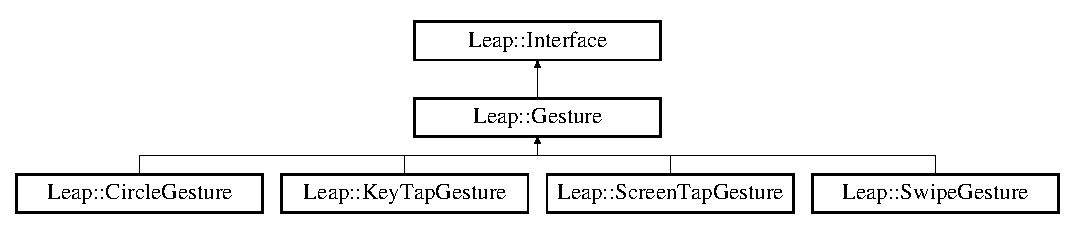
\includegraphics[height=2.625000cm]{class_leap_1_1_gesture}
\end{center}
\end{figure}
\subsection*{Public Types}
\begin{DoxyCompactItemize}
\item 
enum \hyperlink{class_leap_1_1_gesture_a6fa6dd4f28c502f0d55abc6b71c6f9b1}{Type} \{ \\*
\hyperlink{class_leap_1_1_gesture_a6fa6dd4f28c502f0d55abc6b71c6f9b1a743fdf6ff0a893a5b7bf6a56739af618}{T\+Y\+P\+E\+\_\+\+I\+N\+V\+A\+L\+I\+D} = -\/1, 
\hyperlink{class_leap_1_1_gesture_a6fa6dd4f28c502f0d55abc6b71c6f9b1a0845a054bc76e298900d3bd735d26c9c}{T\+Y\+P\+E\+\_\+\+S\+W\+I\+P\+E} = 1, 
\hyperlink{class_leap_1_1_gesture_a6fa6dd4f28c502f0d55abc6b71c6f9b1a32c2a26d674d97f9c9b2e72569ff6869}{T\+Y\+P\+E\+\_\+\+C\+I\+R\+C\+L\+E} = 4, 
\hyperlink{class_leap_1_1_gesture_a6fa6dd4f28c502f0d55abc6b71c6f9b1aa099d1aa238c369e5b2519f2aaca2218}{T\+Y\+P\+E\+\_\+\+S\+C\+R\+E\+E\+N\+\_\+\+T\+A\+P} = 5, 
\\*
\hyperlink{class_leap_1_1_gesture_a6fa6dd4f28c502f0d55abc6b71c6f9b1a4db232d45dfde82ff0c319f623cc3471}{T\+Y\+P\+E\+\_\+\+K\+E\+Y\+\_\+\+T\+A\+P} = 6
 \}
\item 
enum \hyperlink{class_leap_1_1_gesture_a068c6f3ba05970dc557b62a366073578}{State} \{ \hyperlink{class_leap_1_1_gesture_a068c6f3ba05970dc557b62a366073578a6a15c3a18402c69bd711b58e6dea5d93}{S\+T\+A\+T\+E\+\_\+\+I\+N\+V\+A\+L\+I\+D} = -\/1, 
\hyperlink{class_leap_1_1_gesture_a068c6f3ba05970dc557b62a366073578aae7d6cacedcd2850cdea7d9f2dfd33a4}{S\+T\+A\+T\+E\+\_\+\+S\+T\+A\+R\+T} = 1, 
\hyperlink{class_leap_1_1_gesture_a068c6f3ba05970dc557b62a366073578ac8600576e553a806c9c4a337e5cee473}{S\+T\+A\+T\+E\+\_\+\+U\+P\+D\+A\+T\+E} = 2, 
\hyperlink{class_leap_1_1_gesture_a068c6f3ba05970dc557b62a366073578a4cfb4482ef179e4527c15188328b894f}{S\+T\+A\+T\+E\+\_\+\+S\+T\+O\+P} = 3
 \}
\end{DoxyCompactItemize}
\subsection*{Public Member Functions}
\begin{DoxyCompactItemize}
\item 
\hypertarget{class_leap_1_1_gesture_a5050476dcb08d43618d82aabdf8d95f3}{{\bfseries Gesture} (Gesture\+Implementation $\ast$)}\label{class_leap_1_1_gesture_a5050476dcb08d43618d82aabdf8d95f3}

\item 
L\+E\+A\+P\+\_\+\+E\+X\+P\+O\+R\+T \hyperlink{class_leap_1_1_gesture_a703b6671d33d74dd5669b38e9c2edb15}{Gesture} ()
\item 
L\+E\+A\+P\+\_\+\+E\+X\+P\+O\+R\+T \hyperlink{class_leap_1_1_gesture_a958edec008098eabcd1dc93208136c5f}{Gesture} (const \hyperlink{class_leap_1_1_gesture}{Gesture} \&rhs)
\item 
L\+E\+A\+P\+\_\+\+E\+X\+P\+O\+R\+T \hyperlink{class_leap_1_1_gesture_a6fa6dd4f28c502f0d55abc6b71c6f9b1}{Type} \hyperlink{class_leap_1_1_gesture_a961ded36b3f4f72eff342283808c70d5}{type} () const 
\item 
L\+E\+A\+P\+\_\+\+E\+X\+P\+O\+R\+T \hyperlink{class_leap_1_1_gesture_a068c6f3ba05970dc557b62a366073578}{State} \hyperlink{class_leap_1_1_gesture_ae4e9f9b9fcbbe4b8a165009596efa8a0}{state} () const 
\item 
L\+E\+A\+P\+\_\+\+E\+X\+P\+O\+R\+T int32\+\_\+t \hyperlink{class_leap_1_1_gesture_acac877f9c2803f7d7d03107be9348471}{id} () const 
\item 
L\+E\+A\+P\+\_\+\+E\+X\+P\+O\+R\+T int64\+\_\+t \hyperlink{class_leap_1_1_gesture_a9ed79a136da6a2fd65447228274175f3}{duration} () const 
\item 
L\+E\+A\+P\+\_\+\+E\+X\+P\+O\+R\+T float \hyperlink{class_leap_1_1_gesture_a98cf1c2bf86396ec665a652097e61c4f}{duration\+Seconds} () const 
\item 
L\+E\+A\+P\+\_\+\+E\+X\+P\+O\+R\+T \hyperlink{class_leap_1_1_frame}{Frame} \hyperlink{class_leap_1_1_gesture_a44512b16e2d227b9173250c0b1211851}{frame} () const 
\item 
L\+E\+A\+P\+\_\+\+E\+X\+P\+O\+R\+T \hyperlink{class_leap_1_1_hand_list}{Hand\+List} \hyperlink{class_leap_1_1_gesture_a9f8b5383c27efedbc3e47856d865bf21}{hands} () const 
\item 
L\+E\+A\+P\+\_\+\+E\+X\+P\+O\+R\+T \hyperlink{class_leap_1_1_pointable_list}{Pointable\+List} \hyperlink{class_leap_1_1_gesture_a45d8fc212a0b6abfdf05be409b2ba09f}{pointables} () const 
\item 
L\+E\+A\+P\+\_\+\+E\+X\+P\+O\+R\+T bool \hyperlink{class_leap_1_1_gesture_afc32b33f86e676ef854d5298be4f56bd}{is\+Valid} () const 
\item 
L\+E\+A\+P\+\_\+\+E\+X\+P\+O\+R\+T bool \hyperlink{class_leap_1_1_gesture_a13725877525e73592601bd85091cdccb}{operator==} (const \hyperlink{class_leap_1_1_gesture}{Gesture} \&rhs) const 
\item 
L\+E\+A\+P\+\_\+\+E\+X\+P\+O\+R\+T bool \hyperlink{class_leap_1_1_gesture_a795392baacac8bba8661d9487727e547}{operator!=} (const \hyperlink{class_leap_1_1_gesture}{Gesture} \&rhs) const 
\item 
L\+E\+A\+P\+\_\+\+E\+X\+P\+O\+R\+T std\+::string \hyperlink{class_leap_1_1_gesture_a00a3b12d834ce58c004282076cc3ea72}{to\+String} () const 
\end{DoxyCompactItemize}
\subsection*{Static Public Member Functions}
\begin{DoxyCompactItemize}
\item 
static L\+E\+A\+P\+\_\+\+E\+X\+P\+O\+R\+T const \hyperlink{class_leap_1_1_gesture}{Gesture} \& \hyperlink{class_leap_1_1_gesture_a76cbf3abfeb8c1b4fb6faed4483bb185}{invalid} ()
\end{DoxyCompactItemize}
\subsection*{Additional Inherited Members}


\subsection{Detailed Description}
The \hyperlink{class_leap_1_1_gesture}{Gesture} class represents a recognized movement by the user.

The Leap Motion \hyperlink{class_leap_1_1_controller}{Controller} watches the activity within its field of view for certain movement patterns typical of a user gesture or command. For example, a movement from side to side with the hand can indicate a swipe gesture, while a finger poking forward can indicate a screen tap gesture.

When the Leap Motion software recognizes a gesture, it assigns an I\+D and adds a \hyperlink{class_leap_1_1_gesture}{Gesture} object to the frame gesture list. For continuous gestures, which occur over many frames, the Leap Motion software updates the gesture by adding a \hyperlink{class_leap_1_1_gesture}{Gesture} object having the same I\+D and updated properties in each subsequent frame.

{\bfseries Important\+:} Recognition for each type of gesture must be enabled using the \hyperlink{class_leap_1_1_controller_ad24410dee9de51b16ceb6b8c97fe5a36}{Controller\+::enable\+Gesture()} function; otherwise {\bfseries no gestures are recognized or reported}.

Subclasses of \hyperlink{class_leap_1_1_gesture}{Gesture} define the properties for the specific movement patterns recognized by the Leap Motion software.

The \hyperlink{class_leap_1_1_gesture}{Gesture} subclasses for include\+:


\begin{DoxyItemize}
\item \hyperlink{class_leap_1_1_circle_gesture}{Circle\+Gesture} -- A circular movement by a finger.
\item \hyperlink{class_leap_1_1_swipe_gesture}{Swipe\+Gesture} -- A straight line movement by the hand with fingers extended.
\item \hyperlink{class_leap_1_1_screen_tap_gesture}{Screen\+Tap\+Gesture} -- A forward tapping movement by a finger.
\item \hyperlink{class_leap_1_1_key_tap_gesture}{Key\+Tap\+Gesture} -- A downward tapping movement by a finger.
\end{DoxyItemize}

Circle and swipe gestures are continuous and these objects can have a state of start, update, and stop.

The screen tap gesture is a discrete gesture. The Leap Motion software only creates a single \hyperlink{class_leap_1_1_screen_tap_gesture}{Screen\+Tap\+Gesture} object for each tap and it always has a stop state.

Get valid \hyperlink{class_leap_1_1_gesture}{Gesture} instances from a \hyperlink{class_leap_1_1_frame}{Frame} object. You can get a list of gestures with the \hyperlink{class_leap_1_1_frame_a4e4dfb7dbe7796d836fdbec255909379}{Frame\+::gestures()} method. You can get a list of gestures since a specified frame with the {\ttfamily Frame\+::gestures(const Frame\&)} method. You can also use the {\ttfamily \hyperlink{class_leap_1_1_frame_afb0577b99e3bc259c4e20a710062c926}{Frame\+::gesture()}} method to find a gesture in the current frame using an I\+D value obtained in a previous frame.

\hyperlink{class_leap_1_1_gesture}{Gesture} objects can be invalid. For example, when you get a gesture by I\+D using {\ttfamily \hyperlink{class_leap_1_1_frame_afb0577b99e3bc259c4e20a710062c926}{Frame\+::gesture()}}, and there is no gesture with that I\+D in the current frame, then {\ttfamily gesture()} returns an Invalid \hyperlink{class_leap_1_1_gesture}{Gesture} object (rather than a null value). Always check object validity in situations where a gesture might be invalid.

The following keys can be used with the \hyperlink{class_leap_1_1_config}{Config} class to configure the gesture recognizer\+:

\begin{TabularC}{4}
\hline
\rowcolor{lightgray}{\bf Key string }&{\bf Value type }&{\bf Default value }&{\bf Units  }\\\cline{1-4}
Gesture.\+Circle.\+Min\+Radius &float &5.\+0 &mm \\\cline{1-4}
Gesture.\+Circle.\+Min\+Arc &float &1.\+5$\ast$pi &radians \\\cline{1-4}
Gesture.\+Swipe.\+Min\+Length &float &150 &mm \\\cline{1-4}
Gesture.\+Swipe.\+Min\+Velocity &float &1000 &mm/s \\\cline{1-4}
Gesture.\+Key\+Tap.\+Min\+Down\+Velocity &float &50 &mm/s \\\cline{1-4}
Gesture.\+Key\+Tap.\+History\+Seconds &float &0.\+1 &s \\\cline{1-4}
Gesture.\+Key\+Tap.\+Min\+Distance &float &5.\+0 &mm \\\cline{1-4}
Gesture.\+Screen\+Tap.\+Min\+Forward\+Velocity &float &50 &mm/s \\\cline{1-4}
Gesture.\+Screen\+Tap.\+History\+Seconds &float &0.\+1 &s \\\cline{1-4}
Gesture.\+Screen\+Tap.\+Min\+Distance &float &3.\+0 &mm \\\cline{1-4}
\end{TabularC}
\begin{DoxySince}{Since}
1.\+0 
\end{DoxySince}


\subsection{Member Enumeration Documentation}
\hypertarget{class_leap_1_1_gesture_a068c6f3ba05970dc557b62a366073578}{\index{Leap\+::\+Gesture@{Leap\+::\+Gesture}!State@{State}}
\index{State@{State}!Leap\+::\+Gesture@{Leap\+::\+Gesture}}
\subsubsection[{State}]{\setlength{\rightskip}{0pt plus 5cm}enum {\bf Leap\+::\+Gesture\+::\+State}}}\label{class_leap_1_1_gesture_a068c6f3ba05970dc557b62a366073578}
The possible gesture states. \begin{DoxySince}{Since}
1.\+0 
\end{DoxySince}
\begin{Desc}
\item[Enumerator]\par
\begin{description}
\index{S\+T\+A\+T\+E\+\_\+\+I\+N\+V\+A\+L\+I\+D@{S\+T\+A\+T\+E\+\_\+\+I\+N\+V\+A\+L\+I\+D}!Leap\+::\+Gesture@{Leap\+::\+Gesture}}\index{Leap\+::\+Gesture@{Leap\+::\+Gesture}!S\+T\+A\+T\+E\+\_\+\+I\+N\+V\+A\+L\+I\+D@{S\+T\+A\+T\+E\+\_\+\+I\+N\+V\+A\+L\+I\+D}}\item[{\em 
\hypertarget{class_leap_1_1_gesture_a068c6f3ba05970dc557b62a366073578a6a15c3a18402c69bd711b58e6dea5d93}{S\+T\+A\+T\+E\+\_\+\+I\+N\+V\+A\+L\+I\+D}\label{class_leap_1_1_gesture_a068c6f3ba05970dc557b62a366073578a6a15c3a18402c69bd711b58e6dea5d93}
}]An invalid state \begin{DoxySince}{Since}
1.\+0 
\end{DoxySince}
\index{S\+T\+A\+T\+E\+\_\+\+S\+T\+A\+R\+T@{S\+T\+A\+T\+E\+\_\+\+S\+T\+A\+R\+T}!Leap\+::\+Gesture@{Leap\+::\+Gesture}}\index{Leap\+::\+Gesture@{Leap\+::\+Gesture}!S\+T\+A\+T\+E\+\_\+\+S\+T\+A\+R\+T@{S\+T\+A\+T\+E\+\_\+\+S\+T\+A\+R\+T}}\item[{\em 
\hypertarget{class_leap_1_1_gesture_a068c6f3ba05970dc557b62a366073578aae7d6cacedcd2850cdea7d9f2dfd33a4}{S\+T\+A\+T\+E\+\_\+\+S\+T\+A\+R\+T}\label{class_leap_1_1_gesture_a068c6f3ba05970dc557b62a366073578aae7d6cacedcd2850cdea7d9f2dfd33a4}
}]The gesture is starting. Just enough has happened to recognize it. \begin{DoxySince}{Since}
1.\+0 
\end{DoxySince}
\index{S\+T\+A\+T\+E\+\_\+\+U\+P\+D\+A\+T\+E@{S\+T\+A\+T\+E\+\_\+\+U\+P\+D\+A\+T\+E}!Leap\+::\+Gesture@{Leap\+::\+Gesture}}\index{Leap\+::\+Gesture@{Leap\+::\+Gesture}!S\+T\+A\+T\+E\+\_\+\+U\+P\+D\+A\+T\+E@{S\+T\+A\+T\+E\+\_\+\+U\+P\+D\+A\+T\+E}}\item[{\em 
\hypertarget{class_leap_1_1_gesture_a068c6f3ba05970dc557b62a366073578ac8600576e553a806c9c4a337e5cee473}{S\+T\+A\+T\+E\+\_\+\+U\+P\+D\+A\+T\+E}\label{class_leap_1_1_gesture_a068c6f3ba05970dc557b62a366073578ac8600576e553a806c9c4a337e5cee473}
}]The gesture is in progress. (Note\+: not all gestures have updates). \begin{DoxySince}{Since}
1.\+0 
\end{DoxySince}
\index{S\+T\+A\+T\+E\+\_\+\+S\+T\+O\+P@{S\+T\+A\+T\+E\+\_\+\+S\+T\+O\+P}!Leap\+::\+Gesture@{Leap\+::\+Gesture}}\index{Leap\+::\+Gesture@{Leap\+::\+Gesture}!S\+T\+A\+T\+E\+\_\+\+S\+T\+O\+P@{S\+T\+A\+T\+E\+\_\+\+S\+T\+O\+P}}\item[{\em 
\hypertarget{class_leap_1_1_gesture_a068c6f3ba05970dc557b62a366073578a4cfb4482ef179e4527c15188328b894f}{S\+T\+A\+T\+E\+\_\+\+S\+T\+O\+P}\label{class_leap_1_1_gesture_a068c6f3ba05970dc557b62a366073578a4cfb4482ef179e4527c15188328b894f}
}]The gesture has completed or stopped. \begin{DoxySince}{Since}
1.\+0 
\end{DoxySince}
\end{description}
\end{Desc}
\hypertarget{class_leap_1_1_gesture_a6fa6dd4f28c502f0d55abc6b71c6f9b1}{\index{Leap\+::\+Gesture@{Leap\+::\+Gesture}!Type@{Type}}
\index{Type@{Type}!Leap\+::\+Gesture@{Leap\+::\+Gesture}}
\subsubsection[{Type}]{\setlength{\rightskip}{0pt plus 5cm}enum {\bf Leap\+::\+Gesture\+::\+Type}}}\label{class_leap_1_1_gesture_a6fa6dd4f28c502f0d55abc6b71c6f9b1}
The supported types of gestures. \begin{DoxySince}{Since}
1.\+0 
\end{DoxySince}
\begin{Desc}
\item[Enumerator]\par
\begin{description}
\index{T\+Y\+P\+E\+\_\+\+I\+N\+V\+A\+L\+I\+D@{T\+Y\+P\+E\+\_\+\+I\+N\+V\+A\+L\+I\+D}!Leap\+::\+Gesture@{Leap\+::\+Gesture}}\index{Leap\+::\+Gesture@{Leap\+::\+Gesture}!T\+Y\+P\+E\+\_\+\+I\+N\+V\+A\+L\+I\+D@{T\+Y\+P\+E\+\_\+\+I\+N\+V\+A\+L\+I\+D}}\item[{\em 
\hypertarget{class_leap_1_1_gesture_a6fa6dd4f28c502f0d55abc6b71c6f9b1a743fdf6ff0a893a5b7bf6a56739af618}{T\+Y\+P\+E\+\_\+\+I\+N\+V\+A\+L\+I\+D}\label{class_leap_1_1_gesture_a6fa6dd4f28c502f0d55abc6b71c6f9b1a743fdf6ff0a893a5b7bf6a56739af618}
}]An invalid type. \begin{DoxySince}{Since}
1.\+0 
\end{DoxySince}
\index{T\+Y\+P\+E\+\_\+\+S\+W\+I\+P\+E@{T\+Y\+P\+E\+\_\+\+S\+W\+I\+P\+E}!Leap\+::\+Gesture@{Leap\+::\+Gesture}}\index{Leap\+::\+Gesture@{Leap\+::\+Gesture}!T\+Y\+P\+E\+\_\+\+S\+W\+I\+P\+E@{T\+Y\+P\+E\+\_\+\+S\+W\+I\+P\+E}}\item[{\em 
\hypertarget{class_leap_1_1_gesture_a6fa6dd4f28c502f0d55abc6b71c6f9b1a0845a054bc76e298900d3bd735d26c9c}{T\+Y\+P\+E\+\_\+\+S\+W\+I\+P\+E}\label{class_leap_1_1_gesture_a6fa6dd4f28c502f0d55abc6b71c6f9b1a0845a054bc76e298900d3bd735d26c9c}
}]A straight line movement by the hand with fingers extended. \begin{DoxySince}{Since}
1.\+0 
\end{DoxySince}
\index{T\+Y\+P\+E\+\_\+\+C\+I\+R\+C\+L\+E@{T\+Y\+P\+E\+\_\+\+C\+I\+R\+C\+L\+E}!Leap\+::\+Gesture@{Leap\+::\+Gesture}}\index{Leap\+::\+Gesture@{Leap\+::\+Gesture}!T\+Y\+P\+E\+\_\+\+C\+I\+R\+C\+L\+E@{T\+Y\+P\+E\+\_\+\+C\+I\+R\+C\+L\+E}}\item[{\em 
\hypertarget{class_leap_1_1_gesture_a6fa6dd4f28c502f0d55abc6b71c6f9b1a32c2a26d674d97f9c9b2e72569ff6869}{T\+Y\+P\+E\+\_\+\+C\+I\+R\+C\+L\+E}\label{class_leap_1_1_gesture_a6fa6dd4f28c502f0d55abc6b71c6f9b1a32c2a26d674d97f9c9b2e72569ff6869}
}]A circular movement by a finger. \begin{DoxySince}{Since}
1.\+0 
\end{DoxySince}
\index{T\+Y\+P\+E\+\_\+\+S\+C\+R\+E\+E\+N\+\_\+\+T\+A\+P@{T\+Y\+P\+E\+\_\+\+S\+C\+R\+E\+E\+N\+\_\+\+T\+A\+P}!Leap\+::\+Gesture@{Leap\+::\+Gesture}}\index{Leap\+::\+Gesture@{Leap\+::\+Gesture}!T\+Y\+P\+E\+\_\+\+S\+C\+R\+E\+E\+N\+\_\+\+T\+A\+P@{T\+Y\+P\+E\+\_\+\+S\+C\+R\+E\+E\+N\+\_\+\+T\+A\+P}}\item[{\em 
\hypertarget{class_leap_1_1_gesture_a6fa6dd4f28c502f0d55abc6b71c6f9b1aa099d1aa238c369e5b2519f2aaca2218}{T\+Y\+P\+E\+\_\+\+S\+C\+R\+E\+E\+N\+\_\+\+T\+A\+P}\label{class_leap_1_1_gesture_a6fa6dd4f28c502f0d55abc6b71c6f9b1aa099d1aa238c369e5b2519f2aaca2218}
}]A forward tapping movement by a finger. \begin{DoxySince}{Since}
1.\+0 
\end{DoxySince}
\index{T\+Y\+P\+E\+\_\+\+K\+E\+Y\+\_\+\+T\+A\+P@{T\+Y\+P\+E\+\_\+\+K\+E\+Y\+\_\+\+T\+A\+P}!Leap\+::\+Gesture@{Leap\+::\+Gesture}}\index{Leap\+::\+Gesture@{Leap\+::\+Gesture}!T\+Y\+P\+E\+\_\+\+K\+E\+Y\+\_\+\+T\+A\+P@{T\+Y\+P\+E\+\_\+\+K\+E\+Y\+\_\+\+T\+A\+P}}\item[{\em 
\hypertarget{class_leap_1_1_gesture_a6fa6dd4f28c502f0d55abc6b71c6f9b1a4db232d45dfde82ff0c319f623cc3471}{T\+Y\+P\+E\+\_\+\+K\+E\+Y\+\_\+\+T\+A\+P}\label{class_leap_1_1_gesture_a6fa6dd4f28c502f0d55abc6b71c6f9b1a4db232d45dfde82ff0c319f623cc3471}
}]A downward tapping movement by a finger. \begin{DoxySince}{Since}
1.\+0 
\end{DoxySince}
\end{description}
\end{Desc}


\subsection{Constructor \& Destructor Documentation}
\hypertarget{class_leap_1_1_gesture_a703b6671d33d74dd5669b38e9c2edb15}{\index{Leap\+::\+Gesture@{Leap\+::\+Gesture}!Gesture@{Gesture}}
\index{Gesture@{Gesture}!Leap\+::\+Gesture@{Leap\+::\+Gesture}}
\subsubsection[{Gesture}]{\setlength{\rightskip}{0pt plus 5cm}L\+E\+A\+P\+\_\+\+E\+X\+P\+O\+R\+T Leap\+::\+Gesture\+::\+Gesture (
\begin{DoxyParamCaption}
{}
\end{DoxyParamCaption}
)}}\label{class_leap_1_1_gesture_a703b6671d33d74dd5669b38e9c2edb15}
Constructs a new \hyperlink{class_leap_1_1_gesture}{Gesture} object.

An uninitialized \hyperlink{class_leap_1_1_gesture}{Gesture} object is considered invalid. Get valid instances of the \hyperlink{class_leap_1_1_gesture}{Gesture} class, which will be one of the \hyperlink{class_leap_1_1_gesture}{Gesture} subclasses, from a \hyperlink{class_leap_1_1_frame}{Frame} object. \begin{DoxySince}{Since}
1.\+0 
\end{DoxySince}
\hypertarget{class_leap_1_1_gesture_a958edec008098eabcd1dc93208136c5f}{\index{Leap\+::\+Gesture@{Leap\+::\+Gesture}!Gesture@{Gesture}}
\index{Gesture@{Gesture}!Leap\+::\+Gesture@{Leap\+::\+Gesture}}
\subsubsection[{Gesture}]{\setlength{\rightskip}{0pt plus 5cm}L\+E\+A\+P\+\_\+\+E\+X\+P\+O\+R\+T Leap\+::\+Gesture\+::\+Gesture (
\begin{DoxyParamCaption}
\item[{const {\bf Gesture} \&}]{rhs}
\end{DoxyParamCaption}
)}}\label{class_leap_1_1_gesture_a958edec008098eabcd1dc93208136c5f}
Constructs a new copy of an \hyperlink{class_leap_1_1_gesture}{Gesture} object. \begin{DoxySince}{Since}
1.\+0 
\end{DoxySince}


\subsection{Member Function Documentation}
\hypertarget{class_leap_1_1_gesture_a9ed79a136da6a2fd65447228274175f3}{\index{Leap\+::\+Gesture@{Leap\+::\+Gesture}!duration@{duration}}
\index{duration@{duration}!Leap\+::\+Gesture@{Leap\+::\+Gesture}}
\subsubsection[{duration}]{\setlength{\rightskip}{0pt plus 5cm}L\+E\+A\+P\+\_\+\+E\+X\+P\+O\+R\+T int64\+\_\+t Leap\+::\+Gesture\+::duration (
\begin{DoxyParamCaption}
{}
\end{DoxyParamCaption}
) const}}\label{class_leap_1_1_gesture_a9ed79a136da6a2fd65447228274175f3}
The elapsed duration of the recognized movement up to the frame containing this \hyperlink{class_leap_1_1_gesture}{Gesture} object, in microseconds.

The duration reported for the first \hyperlink{class_leap_1_1_gesture}{Gesture} in the sequence (with the S\+T\+A\+T\+E\+\_\+\+S\+T\+A\+R\+T state) will typically be a small positive number since the movement must progress far enough for the Leap Motion software to recognize it as an intentional gesture.

\begin{DoxyReturn}{Returns}
int64\+\_\+t the elapsed duration in microseconds. 
\end{DoxyReturn}
\begin{DoxySince}{Since}
1.\+0 
\end{DoxySince}
\hypertarget{class_leap_1_1_gesture_a98cf1c2bf86396ec665a652097e61c4f}{\index{Leap\+::\+Gesture@{Leap\+::\+Gesture}!duration\+Seconds@{duration\+Seconds}}
\index{duration\+Seconds@{duration\+Seconds}!Leap\+::\+Gesture@{Leap\+::\+Gesture}}
\subsubsection[{duration\+Seconds}]{\setlength{\rightskip}{0pt plus 5cm}L\+E\+A\+P\+\_\+\+E\+X\+P\+O\+R\+T float Leap\+::\+Gesture\+::duration\+Seconds (
\begin{DoxyParamCaption}
{}
\end{DoxyParamCaption}
) const}}\label{class_leap_1_1_gesture_a98cf1c2bf86396ec665a652097e61c4f}
The elapsed duration in seconds. \begin{DoxySeeAlso}{See also}
\hyperlink{class_leap_1_1_gesture_a9ed79a136da6a2fd65447228274175f3}{duration()} 
\end{DoxySeeAlso}
\begin{DoxyReturn}{Returns}
float the elapsed duration in seconds. 
\end{DoxyReturn}
\begin{DoxySince}{Since}
1.\+0 
\end{DoxySince}
\hypertarget{class_leap_1_1_gesture_a44512b16e2d227b9173250c0b1211851}{\index{Leap\+::\+Gesture@{Leap\+::\+Gesture}!frame@{frame}}
\index{frame@{frame}!Leap\+::\+Gesture@{Leap\+::\+Gesture}}
\subsubsection[{frame}]{\setlength{\rightskip}{0pt plus 5cm}L\+E\+A\+P\+\_\+\+E\+X\+P\+O\+R\+T {\bf Frame} Leap\+::\+Gesture\+::frame (
\begin{DoxyParamCaption}
{}
\end{DoxyParamCaption}
) const}}\label{class_leap_1_1_gesture_a44512b16e2d227b9173250c0b1211851}
The \hyperlink{class_leap_1_1_frame}{Frame} containing this \hyperlink{class_leap_1_1_gesture}{Gesture} instance.

\begin{DoxyReturn}{Returns}
\hyperlink{class_leap_1_1_frame}{Frame} The parent \hyperlink{class_leap_1_1_frame}{Frame} object. 
\end{DoxyReturn}
\begin{DoxySince}{Since}
1.\+0 
\end{DoxySince}
\hypertarget{class_leap_1_1_gesture_a9f8b5383c27efedbc3e47856d865bf21}{\index{Leap\+::\+Gesture@{Leap\+::\+Gesture}!hands@{hands}}
\index{hands@{hands}!Leap\+::\+Gesture@{Leap\+::\+Gesture}}
\subsubsection[{hands}]{\setlength{\rightskip}{0pt plus 5cm}L\+E\+A\+P\+\_\+\+E\+X\+P\+O\+R\+T {\bf Hand\+List} Leap\+::\+Gesture\+::hands (
\begin{DoxyParamCaption}
{}
\end{DoxyParamCaption}
) const}}\label{class_leap_1_1_gesture_a9f8b5383c27efedbc3e47856d865bf21}
The list of hands associated with this \hyperlink{class_leap_1_1_gesture}{Gesture}, if any.

If no hands are related to this gesture, the list is empty.

\begin{DoxyReturn}{Returns}
\hyperlink{class_leap_1_1_hand_list}{Hand\+List} the list of related \hyperlink{class_leap_1_1_hand}{Hand} objects. 
\end{DoxyReturn}
\begin{DoxySince}{Since}
1.\+0 
\end{DoxySince}
\hypertarget{class_leap_1_1_gesture_acac877f9c2803f7d7d03107be9348471}{\index{Leap\+::\+Gesture@{Leap\+::\+Gesture}!id@{id}}
\index{id@{id}!Leap\+::\+Gesture@{Leap\+::\+Gesture}}
\subsubsection[{id}]{\setlength{\rightskip}{0pt plus 5cm}L\+E\+A\+P\+\_\+\+E\+X\+P\+O\+R\+T int32\+\_\+t Leap\+::\+Gesture\+::id (
\begin{DoxyParamCaption}
{}
\end{DoxyParamCaption}
) const}}\label{class_leap_1_1_gesture_acac877f9c2803f7d7d03107be9348471}
The gesture I\+D.

All \hyperlink{class_leap_1_1_gesture}{Gesture} objects belonging to the same recognized movement share the same I\+D value. Use the I\+D value with the \hyperlink{class_leap_1_1_frame_afb0577b99e3bc259c4e20a710062c926}{Frame\+::gesture()} method to find updates related to this \hyperlink{class_leap_1_1_gesture}{Gesture} object in subsequent frames.

\begin{DoxyReturn}{Returns}
int32\+\_\+t the I\+D of this \hyperlink{class_leap_1_1_gesture}{Gesture}. 
\end{DoxyReturn}
\begin{DoxySince}{Since}
1.\+0 
\end{DoxySince}
\hypertarget{class_leap_1_1_gesture_a76cbf3abfeb8c1b4fb6faed4483bb185}{\index{Leap\+::\+Gesture@{Leap\+::\+Gesture}!invalid@{invalid}}
\index{invalid@{invalid}!Leap\+::\+Gesture@{Leap\+::\+Gesture}}
\subsubsection[{invalid}]{\setlength{\rightskip}{0pt plus 5cm}static L\+E\+A\+P\+\_\+\+E\+X\+P\+O\+R\+T const {\bf Gesture}\& Leap\+::\+Gesture\+::invalid (
\begin{DoxyParamCaption}
{}
\end{DoxyParamCaption}
)\hspace{0.3cm}{\ttfamily [static]}}}\label{class_leap_1_1_gesture_a76cbf3abfeb8c1b4fb6faed4483bb185}
Returns an invalid \hyperlink{class_leap_1_1_gesture}{Gesture} object.

You can use the instance returned by this function in comparisons testing whether a given \hyperlink{class_leap_1_1_gesture}{Gesture} instance is valid or invalid. (You can also use the \hyperlink{class_leap_1_1_gesture_afc32b33f86e676ef854d5298be4f56bd}{Gesture\+::is\+Valid()} function.)

\begin{DoxyReturn}{Returns}
The invalid \hyperlink{class_leap_1_1_gesture}{Gesture} instance. 
\end{DoxyReturn}
\begin{DoxySince}{Since}
1.\+0 
\end{DoxySince}
\hypertarget{class_leap_1_1_gesture_afc32b33f86e676ef854d5298be4f56bd}{\index{Leap\+::\+Gesture@{Leap\+::\+Gesture}!is\+Valid@{is\+Valid}}
\index{is\+Valid@{is\+Valid}!Leap\+::\+Gesture@{Leap\+::\+Gesture}}
\subsubsection[{is\+Valid}]{\setlength{\rightskip}{0pt plus 5cm}L\+E\+A\+P\+\_\+\+E\+X\+P\+O\+R\+T bool Leap\+::\+Gesture\+::is\+Valid (
\begin{DoxyParamCaption}
{}
\end{DoxyParamCaption}
) const}}\label{class_leap_1_1_gesture_afc32b33f86e676ef854d5298be4f56bd}
Reports whether this \hyperlink{class_leap_1_1_gesture}{Gesture} instance represents a valid \hyperlink{class_leap_1_1_gesture}{Gesture}.

An invalid \hyperlink{class_leap_1_1_gesture}{Gesture} object does not represent a snapshot of a recognized movement. Invalid \hyperlink{class_leap_1_1_gesture}{Gesture} objects are returned when a valid object cannot be provided. For example, when you get an gesture by I\+D using \hyperlink{class_leap_1_1_frame_afb0577b99e3bc259c4e20a710062c926}{Frame\+::gesture()}, and there is no gesture with that I\+D in the current frame, then gesture() returns an Invalid \hyperlink{class_leap_1_1_gesture}{Gesture} object (rather than a null value). Always check object validity in situations where an gesture might be invalid.

\begin{DoxyReturn}{Returns}
bool True, if this is a valid \hyperlink{class_leap_1_1_gesture}{Gesture} instance; false, otherwise. 
\end{DoxyReturn}
\begin{DoxySince}{Since}
1.\+0 
\end{DoxySince}
\hypertarget{class_leap_1_1_gesture_a795392baacac8bba8661d9487727e547}{\index{Leap\+::\+Gesture@{Leap\+::\+Gesture}!operator"!=@{operator"!=}}
\index{operator"!=@{operator"!=}!Leap\+::\+Gesture@{Leap\+::\+Gesture}}
\subsubsection[{operator"!=}]{\setlength{\rightskip}{0pt plus 5cm}L\+E\+A\+P\+\_\+\+E\+X\+P\+O\+R\+T bool Leap\+::\+Gesture\+::operator!= (
\begin{DoxyParamCaption}
\item[{const {\bf Gesture} \&}]{rhs}
\end{DoxyParamCaption}
) const}}\label{class_leap_1_1_gesture_a795392baacac8bba8661d9487727e547}
Compare \hyperlink{class_leap_1_1_gesture}{Gesture} object inequality.

Two Gestures are equal only if they represent the same snapshot of the same recognized movement. \begin{DoxySince}{Since}
1.\+0 
\end{DoxySince}
\hypertarget{class_leap_1_1_gesture_a13725877525e73592601bd85091cdccb}{\index{Leap\+::\+Gesture@{Leap\+::\+Gesture}!operator==@{operator==}}
\index{operator==@{operator==}!Leap\+::\+Gesture@{Leap\+::\+Gesture}}
\subsubsection[{operator==}]{\setlength{\rightskip}{0pt plus 5cm}L\+E\+A\+P\+\_\+\+E\+X\+P\+O\+R\+T bool Leap\+::\+Gesture\+::operator== (
\begin{DoxyParamCaption}
\item[{const {\bf Gesture} \&}]{rhs}
\end{DoxyParamCaption}
) const}}\label{class_leap_1_1_gesture_a13725877525e73592601bd85091cdccb}
Compare \hyperlink{class_leap_1_1_gesture}{Gesture} object equality.

Two Gestures are equal if they represent the same snapshot of the same recognized movement. \begin{DoxySince}{Since}
1.\+0 
\end{DoxySince}
\hypertarget{class_leap_1_1_gesture_a45d8fc212a0b6abfdf05be409b2ba09f}{\index{Leap\+::\+Gesture@{Leap\+::\+Gesture}!pointables@{pointables}}
\index{pointables@{pointables}!Leap\+::\+Gesture@{Leap\+::\+Gesture}}
\subsubsection[{pointables}]{\setlength{\rightskip}{0pt plus 5cm}L\+E\+A\+P\+\_\+\+E\+X\+P\+O\+R\+T {\bf Pointable\+List} Leap\+::\+Gesture\+::pointables (
\begin{DoxyParamCaption}
{}
\end{DoxyParamCaption}
) const}}\label{class_leap_1_1_gesture_a45d8fc212a0b6abfdf05be409b2ba09f}
The list of fingers and tools associated with this \hyperlink{class_leap_1_1_gesture}{Gesture}, if any.

If no \hyperlink{class_leap_1_1_pointable}{Pointable} objects are related to this gesture, the list is empty.

\begin{DoxyReturn}{Returns}
\hyperlink{class_leap_1_1_pointable_list}{Pointable\+List} the list of related \hyperlink{class_leap_1_1_pointable}{Pointable} objects. 
\end{DoxyReturn}
\begin{DoxySince}{Since}
1.\+0 
\end{DoxySince}
\hypertarget{class_leap_1_1_gesture_ae4e9f9b9fcbbe4b8a165009596efa8a0}{\index{Leap\+::\+Gesture@{Leap\+::\+Gesture}!state@{state}}
\index{state@{state}!Leap\+::\+Gesture@{Leap\+::\+Gesture}}
\subsubsection[{state}]{\setlength{\rightskip}{0pt plus 5cm}L\+E\+A\+P\+\_\+\+E\+X\+P\+O\+R\+T {\bf State} Leap\+::\+Gesture\+::state (
\begin{DoxyParamCaption}
{}
\end{DoxyParamCaption}
) const}}\label{class_leap_1_1_gesture_ae4e9f9b9fcbbe4b8a165009596efa8a0}
The gesture state.

Recognized movements occur over time and have a beginning, a middle, and an end. The '\hyperlink{class_leap_1_1_gesture_ae4e9f9b9fcbbe4b8a165009596efa8a0}{state()}' attribute reports where in that sequence this \hyperlink{class_leap_1_1_gesture}{Gesture} object falls.

\begin{DoxyReturn}{Returns}
\hyperlink{class_leap_1_1_gesture_a068c6f3ba05970dc557b62a366073578}{Gesture\+::\+State} A value from the \hyperlink{class_leap_1_1_gesture_a068c6f3ba05970dc557b62a366073578}{Gesture\+::\+State} enumeration. 
\end{DoxyReturn}
\begin{DoxySince}{Since}
1.\+0 
\end{DoxySince}
\hypertarget{class_leap_1_1_gesture_a00a3b12d834ce58c004282076cc3ea72}{\index{Leap\+::\+Gesture@{Leap\+::\+Gesture}!to\+String@{to\+String}}
\index{to\+String@{to\+String}!Leap\+::\+Gesture@{Leap\+::\+Gesture}}
\subsubsection[{to\+String}]{\setlength{\rightskip}{0pt plus 5cm}L\+E\+A\+P\+\_\+\+E\+X\+P\+O\+R\+T std\+::string Leap\+::\+Gesture\+::to\+String (
\begin{DoxyParamCaption}
{}
\end{DoxyParamCaption}
) const}}\label{class_leap_1_1_gesture_a00a3b12d834ce58c004282076cc3ea72}
A string containing a brief, human-\/readable description of this \hyperlink{class_leap_1_1_gesture}{Gesture}. \begin{DoxySince}{Since}
1.\+0 
\end{DoxySince}
\hypertarget{class_leap_1_1_gesture_a961ded36b3f4f72eff342283808c70d5}{\index{Leap\+::\+Gesture@{Leap\+::\+Gesture}!type@{type}}
\index{type@{type}!Leap\+::\+Gesture@{Leap\+::\+Gesture}}
\subsubsection[{type}]{\setlength{\rightskip}{0pt plus 5cm}L\+E\+A\+P\+\_\+\+E\+X\+P\+O\+R\+T {\bf Type} Leap\+::\+Gesture\+::type (
\begin{DoxyParamCaption}
{}
\end{DoxyParamCaption}
) const}}\label{class_leap_1_1_gesture_a961ded36b3f4f72eff342283808c70d5}
The gesture type.

\begin{DoxyReturn}{Returns}
\hyperlink{class_leap_1_1_gesture_a6fa6dd4f28c502f0d55abc6b71c6f9b1}{Gesture\+::\+Type} A value from the \hyperlink{class_leap_1_1_gesture_a6fa6dd4f28c502f0d55abc6b71c6f9b1}{Gesture\+::\+Type} enumeration. 
\end{DoxyReturn}
\begin{DoxySince}{Since}
1.\+0 
\end{DoxySince}


The documentation for this class was generated from the following file\+:\begin{DoxyCompactItemize}
\item 
Interface\+Managers/Leap.\+h\end{DoxyCompactItemize}

\hypertarget{class_leap_1_1_gesture_list}{\section{Leap\+:\+:Gesture\+List Class Reference}
\label{class_leap_1_1_gesture_list}\index{Leap\+::\+Gesture\+List@{Leap\+::\+Gesture\+List}}
}


{\ttfamily \#include $<$Leap.\+h$>$}

Inheritance diagram for Leap\+:\+:Gesture\+List\+:\begin{figure}[H]
\begin{center}
\leavevmode
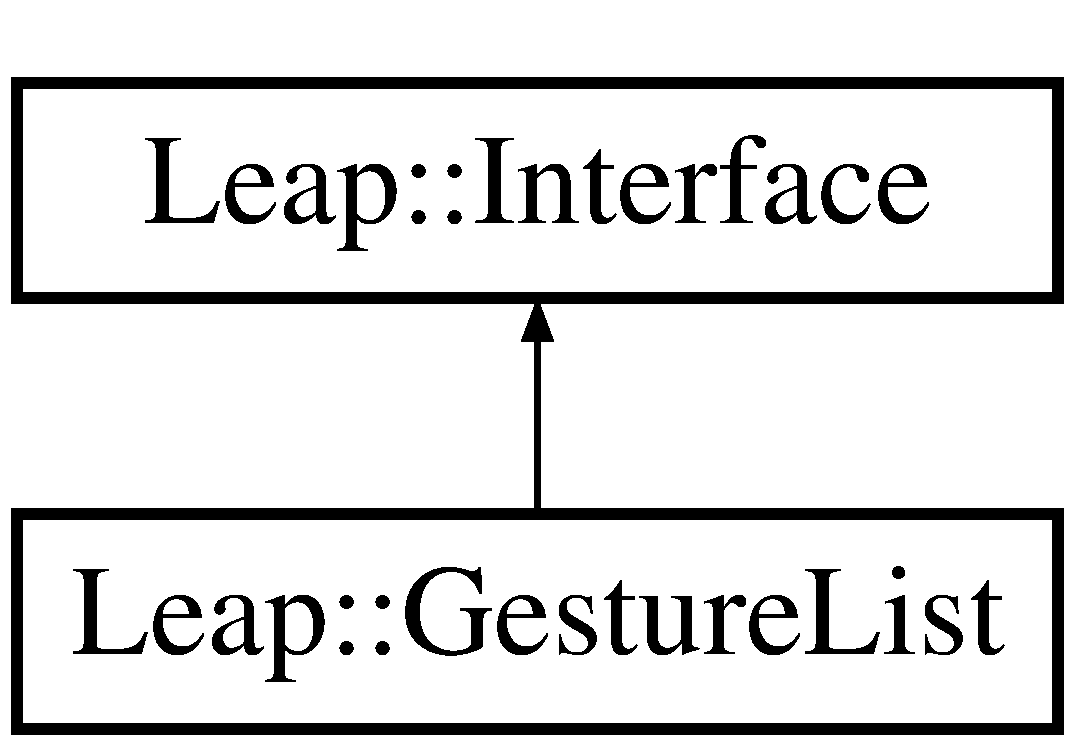
\includegraphics[height=2.000000cm]{class_leap_1_1_gesture_list}
\end{center}
\end{figure}
\subsection*{Public Types}
\begin{DoxyCompactItemize}
\item 
typedef \hyperlink{class_leap_1_1_const_list_iterator}{Const\+List\+Iterator}\\*
$<$ \hyperlink{class_leap_1_1_gesture_list}{Gesture\+List}, \hyperlink{class_leap_1_1_gesture}{Gesture} $>$ \hyperlink{class_leap_1_1_gesture_list_aaf2fd030e686892a0da42d81fc0cad88}{const\+\_\+iterator}
\end{DoxyCompactItemize}
\subsection*{Public Member Functions}
\begin{DoxyCompactItemize}
\item 
\hypertarget{class_leap_1_1_gesture_list_ac514c84e0d23171471f803354b933044}{{\bfseries Gesture\+List} (const \hyperlink{class_leap_1_1_list_base_implementation}{List\+Base\+Implementation}$<$ \hyperlink{class_leap_1_1_gesture}{Gesture} $>$ \&)}\label{class_leap_1_1_gesture_list_ac514c84e0d23171471f803354b933044}

\item 
L\+E\+A\+P\+\_\+\+E\+X\+P\+O\+R\+T \hyperlink{class_leap_1_1_gesture_list_aad564fe5be92fb93119da56f08963142}{Gesture\+List} ()
\item 
L\+E\+A\+P\+\_\+\+E\+X\+P\+O\+R\+T int \hyperlink{class_leap_1_1_gesture_list_afd1d3dc2a25c58971268854f69fdbd2b}{count} () const 
\item 
L\+E\+A\+P\+\_\+\+E\+X\+P\+O\+R\+T bool \hyperlink{class_leap_1_1_gesture_list_a78d661b2023275efa32e3a4f25f45c18}{is\+Empty} () const 
\item 
L\+E\+A\+P\+\_\+\+E\+X\+P\+O\+R\+T \hyperlink{class_leap_1_1_gesture}{Gesture} \hyperlink{class_leap_1_1_gesture_list_ab033b8dc70c9f5e22ae3a24b070d3ff7}{operator\mbox{[}$\,$\mbox{]}} (int index) const 
\item 
L\+E\+A\+P\+\_\+\+E\+X\+P\+O\+R\+T \hyperlink{class_leap_1_1_gesture_list}{Gesture\+List} \& \hyperlink{class_leap_1_1_gesture_list_a377880f99549807dc965087ca14e34f1}{append} (const \hyperlink{class_leap_1_1_gesture_list}{Gesture\+List} \&other)
\item 
L\+E\+A\+P\+\_\+\+E\+X\+P\+O\+R\+T \hyperlink{class_leap_1_1_gesture_list_aaf2fd030e686892a0da42d81fc0cad88}{const\+\_\+iterator} \hyperlink{class_leap_1_1_gesture_list_a1bdcb355a35074a9155581f9ab3aa191}{begin} () const 
\item 
L\+E\+A\+P\+\_\+\+E\+X\+P\+O\+R\+T \hyperlink{class_leap_1_1_gesture_list_aaf2fd030e686892a0da42d81fc0cad88}{const\+\_\+iterator} \hyperlink{class_leap_1_1_gesture_list_adcf2569b3e79c64fd70e02514058559d}{end} () const 
\end{DoxyCompactItemize}
\subsection*{Additional Inherited Members}


\subsection{Detailed Description}
The \hyperlink{class_leap_1_1_gesture_list}{Gesture\+List} class represents a list of \hyperlink{class_leap_1_1_gesture}{Gesture} objects.

Get a \hyperlink{class_leap_1_1_gesture_list}{Gesture\+List} object from a \hyperlink{class_leap_1_1_frame}{Frame} object. \begin{DoxySince}{Since}
1.\+0 
\end{DoxySince}


\subsection{Member Typedef Documentation}
\hypertarget{class_leap_1_1_gesture_list_aaf2fd030e686892a0da42d81fc0cad88}{\index{Leap\+::\+Gesture\+List@{Leap\+::\+Gesture\+List}!const\+\_\+iterator@{const\+\_\+iterator}}
\index{const\+\_\+iterator@{const\+\_\+iterator}!Leap\+::\+Gesture\+List@{Leap\+::\+Gesture\+List}}
\subsubsection[{const\+\_\+iterator}]{\setlength{\rightskip}{0pt plus 5cm}typedef {\bf Const\+List\+Iterator}$<${\bf Gesture\+List}, {\bf Gesture}$>$ {\bf Leap\+::\+Gesture\+List\+::const\+\_\+iterator}}}\label{class_leap_1_1_gesture_list_aaf2fd030e686892a0da42d81fc0cad88}
A C++ iterator type for \hyperlink{class_leap_1_1_gesture_list}{Gesture\+List} objects. \begin{DoxySince}{Since}
1.\+0 
\end{DoxySince}


\subsection{Constructor \& Destructor Documentation}
\hypertarget{class_leap_1_1_gesture_list_aad564fe5be92fb93119da56f08963142}{\index{Leap\+::\+Gesture\+List@{Leap\+::\+Gesture\+List}!Gesture\+List@{Gesture\+List}}
\index{Gesture\+List@{Gesture\+List}!Leap\+::\+Gesture\+List@{Leap\+::\+Gesture\+List}}
\subsubsection[{Gesture\+List}]{\setlength{\rightskip}{0pt plus 5cm}L\+E\+A\+P\+\_\+\+E\+X\+P\+O\+R\+T Leap\+::\+Gesture\+List\+::\+Gesture\+List (
\begin{DoxyParamCaption}
{}
\end{DoxyParamCaption}
)}}\label{class_leap_1_1_gesture_list_aad564fe5be92fb93119da56f08963142}
Constructs an empty gesture list. \begin{DoxySince}{Since}
1.\+0 
\end{DoxySince}


\subsection{Member Function Documentation}
\hypertarget{class_leap_1_1_gesture_list_a377880f99549807dc965087ca14e34f1}{\index{Leap\+::\+Gesture\+List@{Leap\+::\+Gesture\+List}!append@{append}}
\index{append@{append}!Leap\+::\+Gesture\+List@{Leap\+::\+Gesture\+List}}
\subsubsection[{append}]{\setlength{\rightskip}{0pt plus 5cm}L\+E\+A\+P\+\_\+\+E\+X\+P\+O\+R\+T {\bf Gesture\+List}\& Leap\+::\+Gesture\+List\+::append (
\begin{DoxyParamCaption}
\item[{const {\bf Gesture\+List} \&}]{other}
\end{DoxyParamCaption}
)}}\label{class_leap_1_1_gesture_list_a377880f99549807dc965087ca14e34f1}
Appends the members of the specified \hyperlink{class_leap_1_1_gesture_list}{Gesture\+List} to this \hyperlink{class_leap_1_1_gesture_list}{Gesture\+List}. 
\begin{DoxyParams}{Parameters}
{\em other} & A \hyperlink{class_leap_1_1_gesture_list}{Gesture\+List} object containing \hyperlink{class_leap_1_1_gesture}{Gesture} objects to append to the end of this \hyperlink{class_leap_1_1_gesture_list}{Gesture\+List}. \\
\hline
\end{DoxyParams}
\begin{DoxySince}{Since}
1.\+0 
\end{DoxySince}
\hypertarget{class_leap_1_1_gesture_list_a1bdcb355a35074a9155581f9ab3aa191}{\index{Leap\+::\+Gesture\+List@{Leap\+::\+Gesture\+List}!begin@{begin}}
\index{begin@{begin}!Leap\+::\+Gesture\+List@{Leap\+::\+Gesture\+List}}
\subsubsection[{begin}]{\setlength{\rightskip}{0pt plus 5cm}L\+E\+A\+P\+\_\+\+E\+X\+P\+O\+R\+T {\bf const\+\_\+iterator} Leap\+::\+Gesture\+List\+::begin (
\begin{DoxyParamCaption}
{}
\end{DoxyParamCaption}
) const}}\label{class_leap_1_1_gesture_list_a1bdcb355a35074a9155581f9ab3aa191}
The C++ iterator set to the beginning of this \hyperlink{class_leap_1_1_gesture_list}{Gesture\+List}. \begin{DoxySince}{Since}
1.\+0 
\end{DoxySince}
\hypertarget{class_leap_1_1_gesture_list_afd1d3dc2a25c58971268854f69fdbd2b}{\index{Leap\+::\+Gesture\+List@{Leap\+::\+Gesture\+List}!count@{count}}
\index{count@{count}!Leap\+::\+Gesture\+List@{Leap\+::\+Gesture\+List}}
\subsubsection[{count}]{\setlength{\rightskip}{0pt plus 5cm}L\+E\+A\+P\+\_\+\+E\+X\+P\+O\+R\+T int Leap\+::\+Gesture\+List\+::count (
\begin{DoxyParamCaption}
{}
\end{DoxyParamCaption}
) const}}\label{class_leap_1_1_gesture_list_afd1d3dc2a25c58971268854f69fdbd2b}
The length of this list. \begin{DoxyReturn}{Returns}
The number of gestures in this list. 
\end{DoxyReturn}
\begin{DoxySince}{Since}
1.\+0 
\end{DoxySince}
\hypertarget{class_leap_1_1_gesture_list_adcf2569b3e79c64fd70e02514058559d}{\index{Leap\+::\+Gesture\+List@{Leap\+::\+Gesture\+List}!end@{end}}
\index{end@{end}!Leap\+::\+Gesture\+List@{Leap\+::\+Gesture\+List}}
\subsubsection[{end}]{\setlength{\rightskip}{0pt plus 5cm}L\+E\+A\+P\+\_\+\+E\+X\+P\+O\+R\+T {\bf const\+\_\+iterator} Leap\+::\+Gesture\+List\+::end (
\begin{DoxyParamCaption}
{}
\end{DoxyParamCaption}
) const}}\label{class_leap_1_1_gesture_list_adcf2569b3e79c64fd70e02514058559d}
The C++ iterator set to the end of this \hyperlink{class_leap_1_1_gesture_list}{Gesture\+List}. \begin{DoxySince}{Since}
1.\+0 
\end{DoxySince}
\hypertarget{class_leap_1_1_gesture_list_a78d661b2023275efa32e3a4f25f45c18}{\index{Leap\+::\+Gesture\+List@{Leap\+::\+Gesture\+List}!is\+Empty@{is\+Empty}}
\index{is\+Empty@{is\+Empty}!Leap\+::\+Gesture\+List@{Leap\+::\+Gesture\+List}}
\subsubsection[{is\+Empty}]{\setlength{\rightskip}{0pt plus 5cm}L\+E\+A\+P\+\_\+\+E\+X\+P\+O\+R\+T bool Leap\+::\+Gesture\+List\+::is\+Empty (
\begin{DoxyParamCaption}
{}
\end{DoxyParamCaption}
) const}}\label{class_leap_1_1_gesture_list_a78d661b2023275efa32e3a4f25f45c18}
Reports whether the list is empty. \begin{DoxyReturn}{Returns}
True, if the list has no members. 
\end{DoxyReturn}
\begin{DoxySince}{Since}
1.\+0 
\end{DoxySince}
\hypertarget{class_leap_1_1_gesture_list_ab033b8dc70c9f5e22ae3a24b070d3ff7}{\index{Leap\+::\+Gesture\+List@{Leap\+::\+Gesture\+List}!operator\mbox{[}$\,$\mbox{]}@{operator[]}}
\index{operator\mbox{[}$\,$\mbox{]}@{operator[]}!Leap\+::\+Gesture\+List@{Leap\+::\+Gesture\+List}}
\subsubsection[{operator[]}]{\setlength{\rightskip}{0pt plus 5cm}L\+E\+A\+P\+\_\+\+E\+X\+P\+O\+R\+T {\bf Gesture} Leap\+::\+Gesture\+List\+::operator\mbox{[}$\,$\mbox{]} (
\begin{DoxyParamCaption}
\item[{int}]{index}
\end{DoxyParamCaption}
) const}}\label{class_leap_1_1_gesture_list_ab033b8dc70c9f5e22ae3a24b070d3ff7}
Access a list member by its position in the list. 
\begin{DoxyParams}{Parameters}
{\em index} & The zero-\/based list position index. \\
\hline
\end{DoxyParams}
\begin{DoxyReturn}{Returns}
The \hyperlink{class_leap_1_1_gesture}{Gesture} object at the specified index. 
\end{DoxyReturn}
\begin{DoxySince}{Since}
1.\+0 
\end{DoxySince}


The documentation for this class was generated from the following file\+:\begin{DoxyCompactItemize}
\item 
Interface\+Managers/Leap.\+h\end{DoxyCompactItemize}

\hypertarget{class_leap_1_1_hand}{\section{Leap\+:\+:Hand Class Reference}
\label{class_leap_1_1_hand}\index{Leap\+::\+Hand@{Leap\+::\+Hand}}
}


{\ttfamily \#include $<$Leap.\+h$>$}

Inheritance diagram for Leap\+:\+:Hand\+:\begin{figure}[H]
\begin{center}
\leavevmode
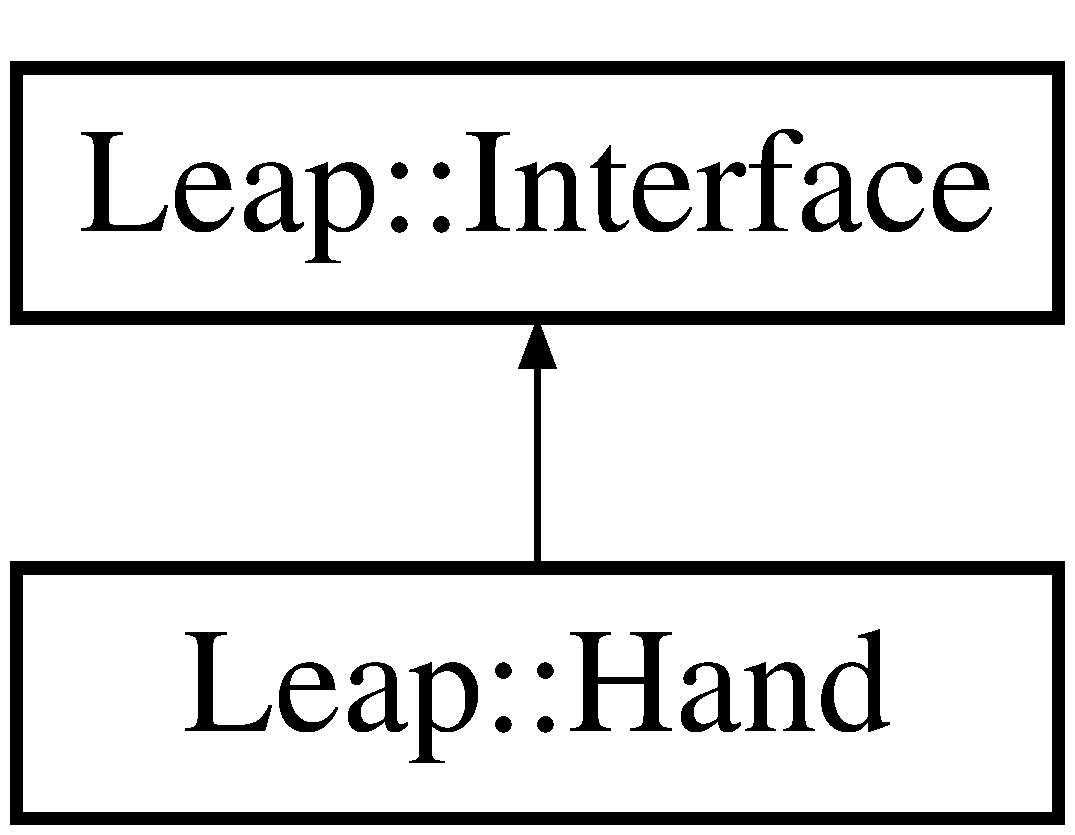
\includegraphics[height=2.000000cm]{class_leap_1_1_hand}
\end{center}
\end{figure}
\subsection*{Public Member Functions}
\begin{DoxyCompactItemize}
\item 
\hypertarget{class_leap_1_1_hand_a52cbd09a5d4f7677d5761d0eafa8c806}{{\bfseries Hand} (Hand\+Implementation $\ast$)}\label{class_leap_1_1_hand_a52cbd09a5d4f7677d5761d0eafa8c806}

\item 
L\+E\+A\+P\+\_\+\+E\+X\+P\+O\+R\+T \hyperlink{class_leap_1_1_hand_a56f41d7f4cded32073c7bec2cebe926d}{Hand} ()
\item 
L\+E\+A\+P\+\_\+\+E\+X\+P\+O\+R\+T int32\+\_\+t \hyperlink{class_leap_1_1_hand_a8df68a42fda7ced114f7112de746e40e}{id} () const 
\item 
L\+E\+A\+P\+\_\+\+E\+X\+P\+O\+R\+T \hyperlink{class_leap_1_1_frame}{Frame} \hyperlink{class_leap_1_1_hand_ad25bf2e94c06bcd8533921059097c95b}{frame} () const 
\item 
L\+E\+A\+P\+\_\+\+E\+X\+P\+O\+R\+T \hyperlink{class_leap_1_1_pointable_list}{Pointable\+List} \hyperlink{class_leap_1_1_hand_a78fa1e5a1134de8802c33d4bc40daee6}{pointables} () const 
\item 
L\+E\+A\+P\+\_\+\+E\+X\+P\+O\+R\+T \hyperlink{class_leap_1_1_pointable}{Pointable} \hyperlink{class_leap_1_1_hand_a93b1c53b8171640c93be27c7c4a3b2cb}{pointable} (int32\+\_\+t \hyperlink{class_leap_1_1_hand_a8df68a42fda7ced114f7112de746e40e}{id}) const 
\item 
L\+E\+A\+P\+\_\+\+E\+X\+P\+O\+R\+T \hyperlink{class_leap_1_1_finger_list}{Finger\+List} \hyperlink{class_leap_1_1_hand_a277253afc4b3e880d9514db5c64c10f2}{fingers} () const 
\item 
L\+E\+A\+P\+\_\+\+E\+X\+P\+O\+R\+T \hyperlink{class_leap_1_1_finger}{Finger} \hyperlink{class_leap_1_1_hand_ae542301c4cb54fd49e0c806089cc152d}{finger} (int32\+\_\+t \hyperlink{class_leap_1_1_hand_a8df68a42fda7ced114f7112de746e40e}{id}) const 
\item 
L\+E\+A\+P\+\_\+\+E\+X\+P\+O\+R\+T \hyperlink{class_leap_1_1_tool_list}{Tool\+List} \hyperlink{class_leap_1_1_hand_afacdaa91afb5bdbe39b37ed50ad8d479}{tools} () const 
\item 
L\+E\+A\+P\+\_\+\+E\+X\+P\+O\+R\+T \hyperlink{class_leap_1_1_tool}{Tool} \hyperlink{class_leap_1_1_hand_aaaeea14295e90b90ea94380c52fa3d85}{tool} (int32\+\_\+t \hyperlink{class_leap_1_1_hand_a8df68a42fda7ced114f7112de746e40e}{id}) const 
\item 
L\+E\+A\+P\+\_\+\+E\+X\+P\+O\+R\+T \hyperlink{struct_leap_1_1_vector}{Vector} \hyperlink{class_leap_1_1_hand_aadb96b762b58cb79fe5f76f4c33c0682}{palm\+Position} () const 
\item 
L\+E\+A\+P\+\_\+\+E\+X\+P\+O\+R\+T \hyperlink{struct_leap_1_1_vector}{Vector} \hyperlink{class_leap_1_1_hand_ab95f0b3e24f0899fe878c755b212503d}{stabilized\+Palm\+Position} () const 
\item 
L\+E\+A\+P\+\_\+\+E\+X\+P\+O\+R\+T \hyperlink{struct_leap_1_1_vector}{Vector} \hyperlink{class_leap_1_1_hand_a990694d00a71b4847c55b8d36042c001}{palm\+Velocity} () const 
\item 
L\+E\+A\+P\+\_\+\+E\+X\+P\+O\+R\+T \hyperlink{struct_leap_1_1_vector}{Vector} \hyperlink{class_leap_1_1_hand_a6e5f1d82f6ae764ec9518088fc73c28a}{palm\+Normal} () const 
\item 
L\+E\+A\+P\+\_\+\+E\+X\+P\+O\+R\+T \hyperlink{struct_leap_1_1_vector}{Vector} \hyperlink{class_leap_1_1_hand_a144acb9740e0706c8c3542043a936b13}{direction} () const 
\item 
L\+E\+A\+P\+\_\+\+E\+X\+P\+O\+R\+T \hyperlink{struct_leap_1_1_vector}{Vector} \hyperlink{class_leap_1_1_hand_a3e614a35a61d6ff3535804ecde25094c}{sphere\+Center} () const 
\item 
L\+E\+A\+P\+\_\+\+E\+X\+P\+O\+R\+T float \hyperlink{class_leap_1_1_hand_a388e8fdcfaa06d0ebba5e207d17d05fd}{sphere\+Radius} () const 
\item 
L\+E\+A\+P\+\_\+\+E\+X\+P\+O\+R\+T \hyperlink{struct_leap_1_1_vector}{Vector} \hyperlink{class_leap_1_1_hand_a4f97a292506e9f90e9d39134008085e0}{translation} (const \hyperlink{class_leap_1_1_frame}{Frame} \&since\+Frame) const 
\item 
L\+E\+A\+P\+\_\+\+E\+X\+P\+O\+R\+T float \hyperlink{class_leap_1_1_hand_a75bee9552fbfe8f06548344736086afc}{translation\+Probability} (const \hyperlink{class_leap_1_1_frame}{Frame} \&since\+Frame) const 
\item 
L\+E\+A\+P\+\_\+\+E\+X\+P\+O\+R\+T \hyperlink{struct_leap_1_1_vector}{Vector} \hyperlink{class_leap_1_1_hand_a1b0693479f9b6d36ae03ac0bbbeeee1a}{rotation\+Axis} (const \hyperlink{class_leap_1_1_frame}{Frame} \&since\+Frame) const 
\item 
L\+E\+A\+P\+\_\+\+E\+X\+P\+O\+R\+T float \hyperlink{class_leap_1_1_hand_a49ba5ded3fcff40e2f17579cf453d34d}{rotation\+Angle} (const \hyperlink{class_leap_1_1_frame}{Frame} \&since\+Frame) const 
\item 
L\+E\+A\+P\+\_\+\+E\+X\+P\+O\+R\+T float \hyperlink{class_leap_1_1_hand_af8f2fe328d53c118fed225a9f19b896d}{rotation\+Angle} (const \hyperlink{class_leap_1_1_frame}{Frame} \&since\+Frame, const \hyperlink{struct_leap_1_1_vector}{Vector} \&axis) const 
\item 
L\+E\+A\+P\+\_\+\+E\+X\+P\+O\+R\+T \hyperlink{struct_leap_1_1_matrix}{Matrix} \hyperlink{class_leap_1_1_hand_a3b1ba5cdfb5fe951efb3ae8e40003dd3}{rotation\+Matrix} (const \hyperlink{class_leap_1_1_frame}{Frame} \&since\+Frame) const 
\item 
L\+E\+A\+P\+\_\+\+E\+X\+P\+O\+R\+T float \hyperlink{class_leap_1_1_hand_ad58c9fca2449308414f1913b0cd1f2ea}{rotation\+Probability} (const \hyperlink{class_leap_1_1_frame}{Frame} \&since\+Frame) const 
\item 
L\+E\+A\+P\+\_\+\+E\+X\+P\+O\+R\+T float \hyperlink{class_leap_1_1_hand_a883f70b457f82c8aec98044f5d804e04}{scale\+Factor} (const \hyperlink{class_leap_1_1_frame}{Frame} \&since\+Frame) const 
\item 
L\+E\+A\+P\+\_\+\+E\+X\+P\+O\+R\+T float \hyperlink{class_leap_1_1_hand_aef4ee9678c91b3736f1a38ab3fdc275c}{scale\+Probability} (const \hyperlink{class_leap_1_1_frame}{Frame} \&since\+Frame) const 
\item 
L\+E\+A\+P\+\_\+\+E\+X\+P\+O\+R\+T float \hyperlink{class_leap_1_1_hand_a1e31a80fae1add698594a69aefecd97e}{time\+Visible} () const 
\item 
L\+E\+A\+P\+\_\+\+E\+X\+P\+O\+R\+T bool \hyperlink{class_leap_1_1_hand_a2beb2a30fd07dbb5816bdd0af832bf75}{is\+Valid} () const 
\item 
L\+E\+A\+P\+\_\+\+E\+X\+P\+O\+R\+T bool \hyperlink{class_leap_1_1_hand_a986929015b89eaf88a5ea2b8dba6b8a8}{operator==} (const \hyperlink{class_leap_1_1_hand}{Hand} \&) const 
\item 
L\+E\+A\+P\+\_\+\+E\+X\+P\+O\+R\+T bool \hyperlink{class_leap_1_1_hand_abaaee341121479a96c249a554dff0272}{operator!=} (const \hyperlink{class_leap_1_1_hand}{Hand} \&) const 
\item 
L\+E\+A\+P\+\_\+\+E\+X\+P\+O\+R\+T std\+::string \hyperlink{class_leap_1_1_hand_aea9df4c2aa365178805648642da8644e}{to\+String} () const 
\end{DoxyCompactItemize}
\subsection*{Static Public Member Functions}
\begin{DoxyCompactItemize}
\item 
static L\+E\+A\+P\+\_\+\+E\+X\+P\+O\+R\+T const \hyperlink{class_leap_1_1_hand}{Hand} \& \hyperlink{class_leap_1_1_hand_ae66c7683d1c179cb3fa1913be320ea6a}{invalid} ()
\end{DoxyCompactItemize}
\subsection*{Friends}
\begin{DoxyCompactItemize}
\item 
L\+E\+A\+P\+\_\+\+E\+X\+P\+O\+R\+T friend std\+::ostream \& \hyperlink{class_leap_1_1_hand_a0b79e476fe0b74207a5d574c4ae4fe3d}{operator$<$$<$} (std\+::ostream \&, const \hyperlink{class_leap_1_1_hand}{Hand} \&)
\end{DoxyCompactItemize}
\subsection*{Additional Inherited Members}


\subsection{Detailed Description}
The \hyperlink{class_leap_1_1_hand}{Hand} class reports the physical characteristics of a detected hand.

\hyperlink{class_leap_1_1_hand}{Hand} tracking data includes a palm position and velocity; vectors for the palm normal and direction to the fingers; properties of a sphere fit to the hand; and lists of the attached fingers and tools.

Note that \hyperlink{class_leap_1_1_hand}{Hand} objects can be invalid, which means that they do not contain valid tracking data and do not correspond to a physical entity. Invalid \hyperlink{class_leap_1_1_hand}{Hand} objects can be the result of asking for a \hyperlink{class_leap_1_1_hand}{Hand} object using an I\+D from an earlier frame when no \hyperlink{class_leap_1_1_hand}{Hand} objects with that I\+D exist in the current frame. A \hyperlink{class_leap_1_1_hand}{Hand} object created from the \hyperlink{class_leap_1_1_hand}{Hand} constructor is also invalid. Test for validity with the \hyperlink{class_leap_1_1_hand_a2beb2a30fd07dbb5816bdd0af832bf75}{Hand\+::is\+Valid()} function. \begin{DoxySince}{Since}
1.\+0 
\end{DoxySince}


\subsection{Constructor \& Destructor Documentation}
\hypertarget{class_leap_1_1_hand_a56f41d7f4cded32073c7bec2cebe926d}{\index{Leap\+::\+Hand@{Leap\+::\+Hand}!Hand@{Hand}}
\index{Hand@{Hand}!Leap\+::\+Hand@{Leap\+::\+Hand}}
\subsubsection[{Hand}]{\setlength{\rightskip}{0pt plus 5cm}L\+E\+A\+P\+\_\+\+E\+X\+P\+O\+R\+T Leap\+::\+Hand\+::\+Hand (
\begin{DoxyParamCaption}
{}
\end{DoxyParamCaption}
)}}\label{class_leap_1_1_hand_a56f41d7f4cded32073c7bec2cebe926d}
Constructs a \hyperlink{class_leap_1_1_hand}{Hand} object.

An uninitialized hand is considered invalid. Get valid \hyperlink{class_leap_1_1_hand}{Hand} objects from a \hyperlink{class_leap_1_1_frame}{Frame} object. \begin{DoxySince}{Since}
1.\+0 
\end{DoxySince}


\subsection{Member Function Documentation}
\hypertarget{class_leap_1_1_hand_a144acb9740e0706c8c3542043a936b13}{\index{Leap\+::\+Hand@{Leap\+::\+Hand}!direction@{direction}}
\index{direction@{direction}!Leap\+::\+Hand@{Leap\+::\+Hand}}
\subsubsection[{direction}]{\setlength{\rightskip}{0pt plus 5cm}L\+E\+A\+P\+\_\+\+E\+X\+P\+O\+R\+T {\bf Vector} Leap\+::\+Hand\+::direction (
\begin{DoxyParamCaption}
{}
\end{DoxyParamCaption}
) const}}\label{class_leap_1_1_hand_a144acb9740e0706c8c3542043a936b13}
The direction from the palm position toward the fingers.

The direction is expressed as a unit vector pointing in the same direction as the directed line from the palm position to the fingers.

\begin{DoxyReturn}{Returns}
The \hyperlink{struct_leap_1_1_vector}{Vector} pointing from the palm position toward the fingers. 
\end{DoxyReturn}
\begin{DoxySince}{Since}
1.\+0 
\end{DoxySince}
\hypertarget{class_leap_1_1_hand_ae542301c4cb54fd49e0c806089cc152d}{\index{Leap\+::\+Hand@{Leap\+::\+Hand}!finger@{finger}}
\index{finger@{finger}!Leap\+::\+Hand@{Leap\+::\+Hand}}
\subsubsection[{finger}]{\setlength{\rightskip}{0pt plus 5cm}L\+E\+A\+P\+\_\+\+E\+X\+P\+O\+R\+T {\bf Finger} Leap\+::\+Hand\+::finger (
\begin{DoxyParamCaption}
\item[{int32\+\_\+t}]{id}
\end{DoxyParamCaption}
) const}}\label{class_leap_1_1_hand_ae542301c4cb54fd49e0c806089cc152d}
The \hyperlink{class_leap_1_1_finger}{Finger} object with the specified I\+D attached to this hand.

Use the \hyperlink{class_leap_1_1_hand_ae542301c4cb54fd49e0c806089cc152d}{Hand\+::finger()} function to retrieve a \hyperlink{class_leap_1_1_finger}{Finger} object attached to this hand using an I\+D value obtained from a previous frame. This function always returns a \hyperlink{class_leap_1_1_finger}{Finger} object, but if no finger with the specified I\+D is present, an invalid \hyperlink{class_leap_1_1_finger}{Finger} object is returned.

Note that I\+D values persist across frames, but only until tracking of a particular object is lost. If tracking of a finger is lost and subsequently regained, the new \hyperlink{class_leap_1_1_finger}{Finger} object representing that finger may have a different I\+D than that representing the finger in an earlier frame.


\begin{DoxyParams}{Parameters}
{\em id} & The I\+D value of a \hyperlink{class_leap_1_1_finger}{Finger} object from a previous frame. \\
\hline
\end{DoxyParams}
\begin{DoxyReturn}{Returns}
The \hyperlink{class_leap_1_1_finger}{Finger} object with the matching I\+D if one exists for this hand in this frame; otherwise, an invalid \hyperlink{class_leap_1_1_finger}{Finger} object is returned. 
\end{DoxyReturn}
\begin{DoxySince}{Since}
1.\+0 
\end{DoxySince}
\hypertarget{class_leap_1_1_hand_a277253afc4b3e880d9514db5c64c10f2}{\index{Leap\+::\+Hand@{Leap\+::\+Hand}!fingers@{fingers}}
\index{fingers@{fingers}!Leap\+::\+Hand@{Leap\+::\+Hand}}
\subsubsection[{fingers}]{\setlength{\rightskip}{0pt plus 5cm}L\+E\+A\+P\+\_\+\+E\+X\+P\+O\+R\+T {\bf Finger\+List} Leap\+::\+Hand\+::fingers (
\begin{DoxyParamCaption}
{}
\end{DoxyParamCaption}
) const}}\label{class_leap_1_1_hand_a277253afc4b3e880d9514db5c64c10f2}
The list of \hyperlink{class_leap_1_1_finger}{Finger} objects detected in this frame that are attached to this hand, given in arbitrary order. The list can be empty if no fingers attached to this hand are detected.

\begin{DoxyReturn}{Returns}
The \hyperlink{class_leap_1_1_finger_list}{Finger\+List} containing all \hyperlink{class_leap_1_1_finger}{Finger} objects attached to this hand. 
\end{DoxyReturn}
\begin{DoxySince}{Since}
1.\+0 
\end{DoxySince}
\hypertarget{class_leap_1_1_hand_ad25bf2e94c06bcd8533921059097c95b}{\index{Leap\+::\+Hand@{Leap\+::\+Hand}!frame@{frame}}
\index{frame@{frame}!Leap\+::\+Hand@{Leap\+::\+Hand}}
\subsubsection[{frame}]{\setlength{\rightskip}{0pt plus 5cm}L\+E\+A\+P\+\_\+\+E\+X\+P\+O\+R\+T {\bf Frame} Leap\+::\+Hand\+::frame (
\begin{DoxyParamCaption}
{}
\end{DoxyParamCaption}
) const}}\label{class_leap_1_1_hand_ad25bf2e94c06bcd8533921059097c95b}
The \hyperlink{class_leap_1_1_frame}{Frame} associated with this \hyperlink{class_leap_1_1_hand}{Hand}.

\begin{DoxyReturn}{Returns}
The associated \hyperlink{class_leap_1_1_frame}{Frame} object, if available; otherwise, an invalid \hyperlink{class_leap_1_1_frame}{Frame} object is returned. 
\end{DoxyReturn}
\begin{DoxySince}{Since}
1.\+0 
\end{DoxySince}
\hypertarget{class_leap_1_1_hand_a8df68a42fda7ced114f7112de746e40e}{\index{Leap\+::\+Hand@{Leap\+::\+Hand}!id@{id}}
\index{id@{id}!Leap\+::\+Hand@{Leap\+::\+Hand}}
\subsubsection[{id}]{\setlength{\rightskip}{0pt plus 5cm}L\+E\+A\+P\+\_\+\+E\+X\+P\+O\+R\+T int32\+\_\+t Leap\+::\+Hand\+::id (
\begin{DoxyParamCaption}
{}
\end{DoxyParamCaption}
) const}}\label{class_leap_1_1_hand_a8df68a42fda7ced114f7112de746e40e}
A unique I\+D assigned to this \hyperlink{class_leap_1_1_hand}{Hand} object, whose value remains the same across consecutive frames while the tracked hand remains visible. If tracking is lost (for example, when a hand is occluded by another hand or when it is withdrawn from or reaches the edge of the Leap Motion \hyperlink{class_leap_1_1_controller}{Controller} field of view), the Leap Motion software may assign a new I\+D when it detects the hand in a future frame.

Use the I\+D value with the \hyperlink{class_leap_1_1_frame_a7565082f9b3cdaf12b620c2e1d278912}{Frame\+::hand()} function to find this \hyperlink{class_leap_1_1_hand}{Hand} object in future frames.

\begin{DoxyReturn}{Returns}
The I\+D of this hand. 
\end{DoxyReturn}
\begin{DoxySince}{Since}
1.\+0 
\end{DoxySince}
\hypertarget{class_leap_1_1_hand_ae66c7683d1c179cb3fa1913be320ea6a}{\index{Leap\+::\+Hand@{Leap\+::\+Hand}!invalid@{invalid}}
\index{invalid@{invalid}!Leap\+::\+Hand@{Leap\+::\+Hand}}
\subsubsection[{invalid}]{\setlength{\rightskip}{0pt plus 5cm}static L\+E\+A\+P\+\_\+\+E\+X\+P\+O\+R\+T const {\bf Hand}\& Leap\+::\+Hand\+::invalid (
\begin{DoxyParamCaption}
{}
\end{DoxyParamCaption}
)\hspace{0.3cm}{\ttfamily [static]}}}\label{class_leap_1_1_hand_ae66c7683d1c179cb3fa1913be320ea6a}
Returns an invalid \hyperlink{class_leap_1_1_hand}{Hand} object.

You can use the instance returned by this function in comparisons testing whether a given \hyperlink{class_leap_1_1_hand}{Hand} instance is valid or invalid. (You can also use the \hyperlink{class_leap_1_1_hand_a2beb2a30fd07dbb5816bdd0af832bf75}{Hand\+::is\+Valid()} function.)

\begin{DoxyReturn}{Returns}
The invalid \hyperlink{class_leap_1_1_hand}{Hand} instance. 
\end{DoxyReturn}
\begin{DoxySince}{Since}
1.\+0 
\end{DoxySince}
\hypertarget{class_leap_1_1_hand_a2beb2a30fd07dbb5816bdd0af832bf75}{\index{Leap\+::\+Hand@{Leap\+::\+Hand}!is\+Valid@{is\+Valid}}
\index{is\+Valid@{is\+Valid}!Leap\+::\+Hand@{Leap\+::\+Hand}}
\subsubsection[{is\+Valid}]{\setlength{\rightskip}{0pt plus 5cm}L\+E\+A\+P\+\_\+\+E\+X\+P\+O\+R\+T bool Leap\+::\+Hand\+::is\+Valid (
\begin{DoxyParamCaption}
{}
\end{DoxyParamCaption}
) const}}\label{class_leap_1_1_hand_a2beb2a30fd07dbb5816bdd0af832bf75}
Reports whether this is a valid \hyperlink{class_leap_1_1_hand}{Hand} object.

\begin{DoxyReturn}{Returns}
True, if this \hyperlink{class_leap_1_1_hand}{Hand} object contains valid tracking data. 
\end{DoxyReturn}
\begin{DoxySince}{Since}
1.\+0 
\end{DoxySince}
\hypertarget{class_leap_1_1_hand_abaaee341121479a96c249a554dff0272}{\index{Leap\+::\+Hand@{Leap\+::\+Hand}!operator"!=@{operator"!=}}
\index{operator"!=@{operator"!=}!Leap\+::\+Hand@{Leap\+::\+Hand}}
\subsubsection[{operator"!=}]{\setlength{\rightskip}{0pt plus 5cm}L\+E\+A\+P\+\_\+\+E\+X\+P\+O\+R\+T bool Leap\+::\+Hand\+::operator!= (
\begin{DoxyParamCaption}
\item[{const {\bf Hand} \&}]{}
\end{DoxyParamCaption}
) const}}\label{class_leap_1_1_hand_abaaee341121479a96c249a554dff0272}
Compare \hyperlink{class_leap_1_1_hand}{Hand} object inequality. Two \hyperlink{class_leap_1_1_hand}{Hand} objects are equal if and only if both \hyperlink{class_leap_1_1_hand}{Hand} objects represent the exact same physical hand in the same frame and both \hyperlink{class_leap_1_1_hand}{Hand} objects are valid. \begin{DoxySince}{Since}
1.\+0 
\end{DoxySince}
\hypertarget{class_leap_1_1_hand_a986929015b89eaf88a5ea2b8dba6b8a8}{\index{Leap\+::\+Hand@{Leap\+::\+Hand}!operator==@{operator==}}
\index{operator==@{operator==}!Leap\+::\+Hand@{Leap\+::\+Hand}}
\subsubsection[{operator==}]{\setlength{\rightskip}{0pt plus 5cm}L\+E\+A\+P\+\_\+\+E\+X\+P\+O\+R\+T bool Leap\+::\+Hand\+::operator== (
\begin{DoxyParamCaption}
\item[{const {\bf Hand} \&}]{}
\end{DoxyParamCaption}
) const}}\label{class_leap_1_1_hand_a986929015b89eaf88a5ea2b8dba6b8a8}
Compare \hyperlink{class_leap_1_1_hand}{Hand} object equality. Two \hyperlink{class_leap_1_1_hand}{Hand} objects are equal if and only if both \hyperlink{class_leap_1_1_hand}{Hand} objects represent the exact same physical hand in the same frame and both \hyperlink{class_leap_1_1_hand}{Hand} objects are valid. \begin{DoxySince}{Since}
1.\+0 
\end{DoxySince}
\hypertarget{class_leap_1_1_hand_a6e5f1d82f6ae764ec9518088fc73c28a}{\index{Leap\+::\+Hand@{Leap\+::\+Hand}!palm\+Normal@{palm\+Normal}}
\index{palm\+Normal@{palm\+Normal}!Leap\+::\+Hand@{Leap\+::\+Hand}}
\subsubsection[{palm\+Normal}]{\setlength{\rightskip}{0pt plus 5cm}L\+E\+A\+P\+\_\+\+E\+X\+P\+O\+R\+T {\bf Vector} Leap\+::\+Hand\+::palm\+Normal (
\begin{DoxyParamCaption}
{}
\end{DoxyParamCaption}
) const}}\label{class_leap_1_1_hand_a6e5f1d82f6ae764ec9518088fc73c28a}
The normal vector to the palm. If your hand is flat, this vector will point downward, or \char`\"{}out\char`\"{} of the front surface of your palm.



The direction is expressed as a unit vector pointing in the same direction as the palm normal (that is, a vector orthogonal to the palm).

\begin{DoxyReturn}{Returns}
The \hyperlink{struct_leap_1_1_vector}{Vector} normal to the plane formed by the palm. 
\end{DoxyReturn}
\begin{DoxySince}{Since}
1.\+0 
\end{DoxySince}
\hypertarget{class_leap_1_1_hand_aadb96b762b58cb79fe5f76f4c33c0682}{\index{Leap\+::\+Hand@{Leap\+::\+Hand}!palm\+Position@{palm\+Position}}
\index{palm\+Position@{palm\+Position}!Leap\+::\+Hand@{Leap\+::\+Hand}}
\subsubsection[{palm\+Position}]{\setlength{\rightskip}{0pt plus 5cm}L\+E\+A\+P\+\_\+\+E\+X\+P\+O\+R\+T {\bf Vector} Leap\+::\+Hand\+::palm\+Position (
\begin{DoxyParamCaption}
{}
\end{DoxyParamCaption}
) const}}\label{class_leap_1_1_hand_aadb96b762b58cb79fe5f76f4c33c0682}
The center position of the palm in millimeters from the Leap Motion \hyperlink{class_leap_1_1_controller}{Controller} origin.

\begin{DoxyReturn}{Returns}
The \hyperlink{struct_leap_1_1_vector}{Vector} representing the coordinates of the palm position. 
\end{DoxyReturn}
\begin{DoxySince}{Since}
1.\+0 
\end{DoxySince}
\hypertarget{class_leap_1_1_hand_a990694d00a71b4847c55b8d36042c001}{\index{Leap\+::\+Hand@{Leap\+::\+Hand}!palm\+Velocity@{palm\+Velocity}}
\index{palm\+Velocity@{palm\+Velocity}!Leap\+::\+Hand@{Leap\+::\+Hand}}
\subsubsection[{palm\+Velocity}]{\setlength{\rightskip}{0pt plus 5cm}L\+E\+A\+P\+\_\+\+E\+X\+P\+O\+R\+T {\bf Vector} Leap\+::\+Hand\+::palm\+Velocity (
\begin{DoxyParamCaption}
{}
\end{DoxyParamCaption}
) const}}\label{class_leap_1_1_hand_a990694d00a71b4847c55b8d36042c001}
The rate of change of the palm position in millimeters/second.

\begin{DoxyReturn}{Returns}
The \hyperlink{struct_leap_1_1_vector}{Vector} representing the coordinates of the palm velocity. 
\end{DoxyReturn}
\begin{DoxySince}{Since}
1.\+0 
\end{DoxySince}
\hypertarget{class_leap_1_1_hand_a93b1c53b8171640c93be27c7c4a3b2cb}{\index{Leap\+::\+Hand@{Leap\+::\+Hand}!pointable@{pointable}}
\index{pointable@{pointable}!Leap\+::\+Hand@{Leap\+::\+Hand}}
\subsubsection[{pointable}]{\setlength{\rightskip}{0pt plus 5cm}L\+E\+A\+P\+\_\+\+E\+X\+P\+O\+R\+T {\bf Pointable} Leap\+::\+Hand\+::pointable (
\begin{DoxyParamCaption}
\item[{int32\+\_\+t}]{id}
\end{DoxyParamCaption}
) const}}\label{class_leap_1_1_hand_a93b1c53b8171640c93be27c7c4a3b2cb}
The \hyperlink{class_leap_1_1_pointable}{Pointable} object with the specified I\+D associated with this hand.

Use the \hyperlink{class_leap_1_1_hand_a93b1c53b8171640c93be27c7c4a3b2cb}{Hand\+::pointable()} function to retrieve a \hyperlink{class_leap_1_1_pointable}{Pointable} object associated with this hand using an I\+D value obtained from a previous frame. This function always returns a \hyperlink{class_leap_1_1_pointable}{Pointable} object, but if no finger or tool with the specified I\+D is present, an invalid \hyperlink{class_leap_1_1_pointable}{Pointable} object is returned.

Note that I\+D values persist across frames, but only until tracking of a particular object is lost. If tracking of a finger or tool is lost and subsequently regained, the new \hyperlink{class_leap_1_1_pointable}{Pointable} object representing that finger or tool may have a different I\+D than that representing the finger or tool in an earlier frame.


\begin{DoxyParams}{Parameters}
{\em id} & The I\+D value of a \hyperlink{class_leap_1_1_pointable}{Pointable} object from a previous frame. \\
\hline
\end{DoxyParams}
\begin{DoxyReturn}{Returns}
The \hyperlink{class_leap_1_1_pointable}{Pointable} object with the matching I\+D if one exists for this hand in this frame; otherwise, an invalid \hyperlink{class_leap_1_1_pointable}{Pointable} object is returned. 
\end{DoxyReturn}
\begin{DoxySince}{Since}
1.\+0 
\end{DoxySince}
\hypertarget{class_leap_1_1_hand_a78fa1e5a1134de8802c33d4bc40daee6}{\index{Leap\+::\+Hand@{Leap\+::\+Hand}!pointables@{pointables}}
\index{pointables@{pointables}!Leap\+::\+Hand@{Leap\+::\+Hand}}
\subsubsection[{pointables}]{\setlength{\rightskip}{0pt plus 5cm}L\+E\+A\+P\+\_\+\+E\+X\+P\+O\+R\+T {\bf Pointable\+List} Leap\+::\+Hand\+::pointables (
\begin{DoxyParamCaption}
{}
\end{DoxyParamCaption}
) const}}\label{class_leap_1_1_hand_a78fa1e5a1134de8802c33d4bc40daee6}
The list of \hyperlink{class_leap_1_1_pointable}{Pointable} objects (fingers and tools) detected in this frame that are associated with this hand, given in arbitrary order. The list can be empty if no fingers or tools associated with this hand are detected.

Use the \hyperlink{class_leap_1_1_pointable_acb22151412f46b6be8b773986452eba8}{Pointable\+::is\+Finger()} function to determine whether or not an item in the list represents a finger. Use the \hyperlink{class_leap_1_1_pointable_ac10f09626b790dd5867411748242c437}{Pointable\+::is\+Tool()} function to determine whether or not an item in the list represents a tool. You can also get only fingers using the \hyperlink{class_leap_1_1_hand_a277253afc4b3e880d9514db5c64c10f2}{Hand\+::fingers()} function or only tools using the \hyperlink{class_leap_1_1_hand_afacdaa91afb5bdbe39b37ed50ad8d479}{Hand\+::tools()} function.

\begin{DoxyReturn}{Returns}
The \hyperlink{class_leap_1_1_pointable_list}{Pointable\+List} containing all \hyperlink{class_leap_1_1_pointable}{Pointable} objects associated with this hand. 
\end{DoxyReturn}
\begin{DoxySince}{Since}
1.\+0 
\end{DoxySince}
\hypertarget{class_leap_1_1_hand_a49ba5ded3fcff40e2f17579cf453d34d}{\index{Leap\+::\+Hand@{Leap\+::\+Hand}!rotation\+Angle@{rotation\+Angle}}
\index{rotation\+Angle@{rotation\+Angle}!Leap\+::\+Hand@{Leap\+::\+Hand}}
\subsubsection[{rotation\+Angle}]{\setlength{\rightskip}{0pt plus 5cm}L\+E\+A\+P\+\_\+\+E\+X\+P\+O\+R\+T float Leap\+::\+Hand\+::rotation\+Angle (
\begin{DoxyParamCaption}
\item[{const {\bf Frame} \&}]{since\+Frame}
\end{DoxyParamCaption}
) const}}\label{class_leap_1_1_hand_a49ba5ded3fcff40e2f17579cf453d34d}
The angle of rotation around the rotation axis derived from the change in orientation of this hand, and any associated fingers and tools, between the current frame and the specified frame.

The returned angle is expressed in radians measured clockwise around the rotation axis (using the right-\/hand rule) between the start and end frames. The value is always between 0 and pi radians (0 and 180 degrees).

If a corresponding \hyperlink{class_leap_1_1_hand}{Hand} object is not found in since\+Frame, or if either this frame or since\+Frame are invalid \hyperlink{class_leap_1_1_frame}{Frame} objects, then the angle of rotation is zero.


\begin{DoxyParams}{Parameters}
{\em since\+Frame} & The starting frame for computing the relative rotation. \\
\hline
\end{DoxyParams}
\begin{DoxyReturn}{Returns}
A positive value representing the heuristically determined rotational change of the hand between the current frame and that specified in the since\+Frame parameter. 
\end{DoxyReturn}
\begin{DoxySince}{Since}
1.\+0 
\end{DoxySince}
\hypertarget{class_leap_1_1_hand_af8f2fe328d53c118fed225a9f19b896d}{\index{Leap\+::\+Hand@{Leap\+::\+Hand}!rotation\+Angle@{rotation\+Angle}}
\index{rotation\+Angle@{rotation\+Angle}!Leap\+::\+Hand@{Leap\+::\+Hand}}
\subsubsection[{rotation\+Angle}]{\setlength{\rightskip}{0pt plus 5cm}L\+E\+A\+P\+\_\+\+E\+X\+P\+O\+R\+T float Leap\+::\+Hand\+::rotation\+Angle (
\begin{DoxyParamCaption}
\item[{const {\bf Frame} \&}]{since\+Frame, }
\item[{const {\bf Vector} \&}]{axis}
\end{DoxyParamCaption}
) const}}\label{class_leap_1_1_hand_af8f2fe328d53c118fed225a9f19b896d}
The angle of rotation around the specified axis derived from the change in orientation of this hand, and any associated fingers and tools, between the current frame and the specified frame.

The returned angle is expressed in radians measured clockwise around the rotation axis (using the right-\/hand rule) between the start and end frames. The value is always between -\/pi and pi radians (-\/180 and 180 degrees).

If a corresponding \hyperlink{class_leap_1_1_hand}{Hand} object is not found in since\+Frame, or if either this frame or since\+Frame are invalid \hyperlink{class_leap_1_1_frame}{Frame} objects, then the angle of rotation is zero.


\begin{DoxyParams}{Parameters}
{\em since\+Frame} & The starting frame for computing the relative rotation. \\
\hline
{\em axis} & The axis to measure rotation around. \\
\hline
\end{DoxyParams}
\begin{DoxyReturn}{Returns}
A value representing the heuristically determined rotational change of the hand between the current frame and that specified in the since\+Frame parameter around the specified axis. 
\end{DoxyReturn}
\begin{DoxySince}{Since}
1.\+0 
\end{DoxySince}
\hypertarget{class_leap_1_1_hand_a1b0693479f9b6d36ae03ac0bbbeeee1a}{\index{Leap\+::\+Hand@{Leap\+::\+Hand}!rotation\+Axis@{rotation\+Axis}}
\index{rotation\+Axis@{rotation\+Axis}!Leap\+::\+Hand@{Leap\+::\+Hand}}
\subsubsection[{rotation\+Axis}]{\setlength{\rightskip}{0pt plus 5cm}L\+E\+A\+P\+\_\+\+E\+X\+P\+O\+R\+T {\bf Vector} Leap\+::\+Hand\+::rotation\+Axis (
\begin{DoxyParamCaption}
\item[{const {\bf Frame} \&}]{since\+Frame}
\end{DoxyParamCaption}
) const}}\label{class_leap_1_1_hand_a1b0693479f9b6d36ae03ac0bbbeeee1a}
The axis of rotation derived from the change in orientation of this hand, and any associated fingers and tools, between the current frame and the specified frame.

The returned direction vector is normalized.

If a corresponding \hyperlink{class_leap_1_1_hand}{Hand} object is not found in since\+Frame, or if either this frame or since\+Frame are invalid \hyperlink{class_leap_1_1_frame}{Frame} objects, then this method returns a zero vector.


\begin{DoxyParams}{Parameters}
{\em since\+Frame} & The starting frame for computing the relative rotation. \\
\hline
\end{DoxyParams}
\begin{DoxyReturn}{Returns}
A normalized direction \hyperlink{struct_leap_1_1_vector}{Vector} representing the heuristically determined axis of rotational change of the hand between the current frame and that specified in the since\+Frame parameter. 
\end{DoxyReturn}
\begin{DoxySince}{Since}
1.\+0 
\end{DoxySince}
\hypertarget{class_leap_1_1_hand_a3b1ba5cdfb5fe951efb3ae8e40003dd3}{\index{Leap\+::\+Hand@{Leap\+::\+Hand}!rotation\+Matrix@{rotation\+Matrix}}
\index{rotation\+Matrix@{rotation\+Matrix}!Leap\+::\+Hand@{Leap\+::\+Hand}}
\subsubsection[{rotation\+Matrix}]{\setlength{\rightskip}{0pt plus 5cm}L\+E\+A\+P\+\_\+\+E\+X\+P\+O\+R\+T {\bf Matrix} Leap\+::\+Hand\+::rotation\+Matrix (
\begin{DoxyParamCaption}
\item[{const {\bf Frame} \&}]{since\+Frame}
\end{DoxyParamCaption}
) const}}\label{class_leap_1_1_hand_a3b1ba5cdfb5fe951efb3ae8e40003dd3}
The transform matrix expressing the rotation derived from the change in orientation of this hand, and any associated fingers and tools, between the current frame and the specified frame.

If a corresponding \hyperlink{class_leap_1_1_hand}{Hand} object is not found in since\+Frame, or if either this frame or since\+Frame are invalid \hyperlink{class_leap_1_1_frame}{Frame} objects, then this method returns an identity matrix.


\begin{DoxyParams}{Parameters}
{\em since\+Frame} & The starting frame for computing the relative rotation. \\
\hline
\end{DoxyParams}
\begin{DoxyReturn}{Returns}
A transformation \hyperlink{struct_leap_1_1_matrix}{Matrix} representing the heuristically determined rotational change of the hand between the current frame and that specified in the since\+Frame parameter. 
\end{DoxyReturn}
\begin{DoxySince}{Since}
1.\+0 
\end{DoxySince}
\hypertarget{class_leap_1_1_hand_ad58c9fca2449308414f1913b0cd1f2ea}{\index{Leap\+::\+Hand@{Leap\+::\+Hand}!rotation\+Probability@{rotation\+Probability}}
\index{rotation\+Probability@{rotation\+Probability}!Leap\+::\+Hand@{Leap\+::\+Hand}}
\subsubsection[{rotation\+Probability}]{\setlength{\rightskip}{0pt plus 5cm}L\+E\+A\+P\+\_\+\+E\+X\+P\+O\+R\+T float Leap\+::\+Hand\+::rotation\+Probability (
\begin{DoxyParamCaption}
\item[{const {\bf Frame} \&}]{since\+Frame}
\end{DoxyParamCaption}
) const}}\label{class_leap_1_1_hand_ad58c9fca2449308414f1913b0cd1f2ea}
The estimated probability that the hand motion between the current frame and the specified frame is intended to be a rotating motion.

If a corresponding \hyperlink{class_leap_1_1_hand}{Hand} object is not found in since\+Frame, or if either this frame or since\+Frame are invalid \hyperlink{class_leap_1_1_frame}{Frame} objects, then this method returns zero.


\begin{DoxyParams}{Parameters}
{\em since\+Frame} & The starting frame for computing the relative rotation. \\
\hline
\end{DoxyParams}
\begin{DoxyReturn}{Returns}
A value between 0 and 1 representing the estimated probability that the hand motion between the current frame and the specified frame is intended to be a rotating motion. 
\end{DoxyReturn}
\begin{DoxySince}{Since}
1.\+0 
\end{DoxySince}
\hypertarget{class_leap_1_1_hand_a883f70b457f82c8aec98044f5d804e04}{\index{Leap\+::\+Hand@{Leap\+::\+Hand}!scale\+Factor@{scale\+Factor}}
\index{scale\+Factor@{scale\+Factor}!Leap\+::\+Hand@{Leap\+::\+Hand}}
\subsubsection[{scale\+Factor}]{\setlength{\rightskip}{0pt plus 5cm}L\+E\+A\+P\+\_\+\+E\+X\+P\+O\+R\+T float Leap\+::\+Hand\+::scale\+Factor (
\begin{DoxyParamCaption}
\item[{const {\bf Frame} \&}]{since\+Frame}
\end{DoxyParamCaption}
) const}}\label{class_leap_1_1_hand_a883f70b457f82c8aec98044f5d804e04}
The scale factor derived from this hand's motion between the current frame and the specified frame.

The scale factor is always positive. A value of 1.\+0 indicates no scaling took place. Values between 0.\+0 and 1.\+0 indicate contraction and values greater than 1.\+0 indicate expansion.

The Leap Motion software derives scaling from the relative inward or outward motion of a hand and its associated fingers and tools (independent of translation and rotation).

If a corresponding \hyperlink{class_leap_1_1_hand}{Hand} object is not found in since\+Frame, or if either this frame or since\+Frame are invalid \hyperlink{class_leap_1_1_frame}{Frame} objects, then this method returns 1.\+0.


\begin{DoxyParams}{Parameters}
{\em since\+Frame} & The starting frame for computing the relative scaling. \\
\hline
\end{DoxyParams}
\begin{DoxyReturn}{Returns}
A positive value representing the heuristically determined scaling change ratio of the hand between the current frame and that specified in the since\+Frame parameter. 
\end{DoxyReturn}
\begin{DoxySince}{Since}
1.\+0 
\end{DoxySince}
\hypertarget{class_leap_1_1_hand_aef4ee9678c91b3736f1a38ab3fdc275c}{\index{Leap\+::\+Hand@{Leap\+::\+Hand}!scale\+Probability@{scale\+Probability}}
\index{scale\+Probability@{scale\+Probability}!Leap\+::\+Hand@{Leap\+::\+Hand}}
\subsubsection[{scale\+Probability}]{\setlength{\rightskip}{0pt plus 5cm}L\+E\+A\+P\+\_\+\+E\+X\+P\+O\+R\+T float Leap\+::\+Hand\+::scale\+Probability (
\begin{DoxyParamCaption}
\item[{const {\bf Frame} \&}]{since\+Frame}
\end{DoxyParamCaption}
) const}}\label{class_leap_1_1_hand_aef4ee9678c91b3736f1a38ab3fdc275c}
The estimated probability that the hand motion between the current frame and the specified frame is intended to be a scaling motion.

If a corresponding \hyperlink{class_leap_1_1_hand}{Hand} object is not found in since\+Frame, or if either this frame or since\+Frame are invalid \hyperlink{class_leap_1_1_frame}{Frame} objects, then this method returns zero.


\begin{DoxyParams}{Parameters}
{\em since\+Frame} & The starting frame for computing the relative scaling. \\
\hline
\end{DoxyParams}
\begin{DoxyReturn}{Returns}
A value between 0 and 1 representing the estimated probability that the hand motion between the current frame and the specified frame is intended to be a scaling motion. 
\end{DoxyReturn}
\begin{DoxySince}{Since}
1.\+0 
\end{DoxySince}
\hypertarget{class_leap_1_1_hand_a3e614a35a61d6ff3535804ecde25094c}{\index{Leap\+::\+Hand@{Leap\+::\+Hand}!sphere\+Center@{sphere\+Center}}
\index{sphere\+Center@{sphere\+Center}!Leap\+::\+Hand@{Leap\+::\+Hand}}
\subsubsection[{sphere\+Center}]{\setlength{\rightskip}{0pt plus 5cm}L\+E\+A\+P\+\_\+\+E\+X\+P\+O\+R\+T {\bf Vector} Leap\+::\+Hand\+::sphere\+Center (
\begin{DoxyParamCaption}
{}
\end{DoxyParamCaption}
) const}}\label{class_leap_1_1_hand_a3e614a35a61d6ff3535804ecde25094c}
The center of a sphere fit to the curvature of this hand.

This sphere is placed roughly as if the hand were holding a ball.



\begin{DoxyReturn}{Returns}
The \hyperlink{struct_leap_1_1_vector}{Vector} representing the center position of the sphere. 
\end{DoxyReturn}
\begin{DoxySince}{Since}
1.\+0 
\end{DoxySince}
\hypertarget{class_leap_1_1_hand_a388e8fdcfaa06d0ebba5e207d17d05fd}{\index{Leap\+::\+Hand@{Leap\+::\+Hand}!sphere\+Radius@{sphere\+Radius}}
\index{sphere\+Radius@{sphere\+Radius}!Leap\+::\+Hand@{Leap\+::\+Hand}}
\subsubsection[{sphere\+Radius}]{\setlength{\rightskip}{0pt plus 5cm}L\+E\+A\+P\+\_\+\+E\+X\+P\+O\+R\+T float Leap\+::\+Hand\+::sphere\+Radius (
\begin{DoxyParamCaption}
{}
\end{DoxyParamCaption}
) const}}\label{class_leap_1_1_hand_a388e8fdcfaa06d0ebba5e207d17d05fd}
The radius of a sphere fit to the curvature of this hand.

This sphere is placed roughly as if the hand were holding a ball. Thus the size of the sphere decreases as the fingers are curled into a fist. \begin{DoxyReturn}{Returns}
The radius of the sphere in millimeters. 
\end{DoxyReturn}
\begin{DoxySince}{Since}
1.\+0 
\end{DoxySince}
\hypertarget{class_leap_1_1_hand_ab95f0b3e24f0899fe878c755b212503d}{\index{Leap\+::\+Hand@{Leap\+::\+Hand}!stabilized\+Palm\+Position@{stabilized\+Palm\+Position}}
\index{stabilized\+Palm\+Position@{stabilized\+Palm\+Position}!Leap\+::\+Hand@{Leap\+::\+Hand}}
\subsubsection[{stabilized\+Palm\+Position}]{\setlength{\rightskip}{0pt plus 5cm}L\+E\+A\+P\+\_\+\+E\+X\+P\+O\+R\+T {\bf Vector} Leap\+::\+Hand\+::stabilized\+Palm\+Position (
\begin{DoxyParamCaption}
{}
\end{DoxyParamCaption}
) const}}\label{class_leap_1_1_hand_ab95f0b3e24f0899fe878c755b212503d}
The stabilized palm position of this \hyperlink{class_leap_1_1_hand}{Hand}.

Smoothing and stabilization is performed in order to make this value more suitable for interaction with 2\+D content. The stabilized position lags behind the palm position by a variable amount, depending primarily on the speed of movement.

\begin{DoxyReturn}{Returns}
A modified palm position of this \hyperlink{class_leap_1_1_hand}{Hand} object with some additional smoothing and stabilization applied. 
\end{DoxyReturn}
\begin{DoxySince}{Since}
1.\+0 
\end{DoxySince}
\hypertarget{class_leap_1_1_hand_a1e31a80fae1add698594a69aefecd97e}{\index{Leap\+::\+Hand@{Leap\+::\+Hand}!time\+Visible@{time\+Visible}}
\index{time\+Visible@{time\+Visible}!Leap\+::\+Hand@{Leap\+::\+Hand}}
\subsubsection[{time\+Visible}]{\setlength{\rightskip}{0pt plus 5cm}L\+E\+A\+P\+\_\+\+E\+X\+P\+O\+R\+T float Leap\+::\+Hand\+::time\+Visible (
\begin{DoxyParamCaption}
{}
\end{DoxyParamCaption}
) const}}\label{class_leap_1_1_hand_a1e31a80fae1add698594a69aefecd97e}
The duration of time this \hyperlink{class_leap_1_1_hand}{Hand} has been visible to the Leap Motion \hyperlink{class_leap_1_1_controller}{Controller}.

\begin{DoxyReturn}{Returns}
The duration (in seconds) that this \hyperlink{class_leap_1_1_hand}{Hand} has been tracked. 
\end{DoxyReturn}
\begin{DoxySince}{Since}
1.\+0 
\end{DoxySince}
\hypertarget{class_leap_1_1_hand_aaaeea14295e90b90ea94380c52fa3d85}{\index{Leap\+::\+Hand@{Leap\+::\+Hand}!tool@{tool}}
\index{tool@{tool}!Leap\+::\+Hand@{Leap\+::\+Hand}}
\subsubsection[{tool}]{\setlength{\rightskip}{0pt plus 5cm}L\+E\+A\+P\+\_\+\+E\+X\+P\+O\+R\+T {\bf Tool} Leap\+::\+Hand\+::tool (
\begin{DoxyParamCaption}
\item[{int32\+\_\+t}]{id}
\end{DoxyParamCaption}
) const}}\label{class_leap_1_1_hand_aaaeea14295e90b90ea94380c52fa3d85}
The \hyperlink{class_leap_1_1_tool}{Tool} object with the specified I\+D held by this hand.

Use the \hyperlink{class_leap_1_1_hand_aaaeea14295e90b90ea94380c52fa3d85}{Hand\+::tool()} function to retrieve a \hyperlink{class_leap_1_1_tool}{Tool} object held by this hand using an I\+D value obtained from a previous frame. This function always returns a \hyperlink{class_leap_1_1_tool}{Tool} object, but if no tool with the specified I\+D is present, an invalid \hyperlink{class_leap_1_1_tool}{Tool} object is returned.

Note that I\+D values persist across frames, but only until tracking of a particular object is lost. If tracking of a tool is lost and subsequently regained, the new \hyperlink{class_leap_1_1_tool}{Tool} object representing that tool may have a different I\+D than that representing the tool in an earlier frame.


\begin{DoxyParams}{Parameters}
{\em id} & The I\+D value of a \hyperlink{class_leap_1_1_tool}{Tool} object from a previous frame. \\
\hline
\end{DoxyParams}
\begin{DoxyReturn}{Returns}
The \hyperlink{class_leap_1_1_tool}{Tool} object with the matching I\+D if one exists for this hand in this frame; otherwise, an invalid \hyperlink{class_leap_1_1_tool}{Tool} object is returned. 
\end{DoxyReturn}
\begin{DoxySince}{Since}
1.\+0 
\end{DoxySince}
\hypertarget{class_leap_1_1_hand_afacdaa91afb5bdbe39b37ed50ad8d479}{\index{Leap\+::\+Hand@{Leap\+::\+Hand}!tools@{tools}}
\index{tools@{tools}!Leap\+::\+Hand@{Leap\+::\+Hand}}
\subsubsection[{tools}]{\setlength{\rightskip}{0pt plus 5cm}L\+E\+A\+P\+\_\+\+E\+X\+P\+O\+R\+T {\bf Tool\+List} Leap\+::\+Hand\+::tools (
\begin{DoxyParamCaption}
{}
\end{DoxyParamCaption}
) const}}\label{class_leap_1_1_hand_afacdaa91afb5bdbe39b37ed50ad8d479}
The list of \hyperlink{class_leap_1_1_tool}{Tool} objects detected in this frame that are held by this hand, given in arbitrary order. The list can be empty if no tools held by this hand are detected.

\begin{DoxyReturn}{Returns}
The \hyperlink{class_leap_1_1_tool_list}{Tool\+List} containing all \hyperlink{class_leap_1_1_tool}{Tool} objects held by this hand. 
\end{DoxyReturn}
\begin{DoxySince}{Since}
1.\+0 
\end{DoxySince}
\hypertarget{class_leap_1_1_hand_aea9df4c2aa365178805648642da8644e}{\index{Leap\+::\+Hand@{Leap\+::\+Hand}!to\+String@{to\+String}}
\index{to\+String@{to\+String}!Leap\+::\+Hand@{Leap\+::\+Hand}}
\subsubsection[{to\+String}]{\setlength{\rightskip}{0pt plus 5cm}L\+E\+A\+P\+\_\+\+E\+X\+P\+O\+R\+T std\+::string Leap\+::\+Hand\+::to\+String (
\begin{DoxyParamCaption}
{}
\end{DoxyParamCaption}
) const}}\label{class_leap_1_1_hand_aea9df4c2aa365178805648642da8644e}
A string containing a brief, human readable description of the \hyperlink{class_leap_1_1_hand}{Hand} object.

\begin{DoxyReturn}{Returns}
A description of the \hyperlink{class_leap_1_1_hand}{Hand} as a string. 
\end{DoxyReturn}
\begin{DoxySince}{Since}
1.\+0 
\end{DoxySince}
\hypertarget{class_leap_1_1_hand_a4f97a292506e9f90e9d39134008085e0}{\index{Leap\+::\+Hand@{Leap\+::\+Hand}!translation@{translation}}
\index{translation@{translation}!Leap\+::\+Hand@{Leap\+::\+Hand}}
\subsubsection[{translation}]{\setlength{\rightskip}{0pt plus 5cm}L\+E\+A\+P\+\_\+\+E\+X\+P\+O\+R\+T {\bf Vector} Leap\+::\+Hand\+::translation (
\begin{DoxyParamCaption}
\item[{const {\bf Frame} \&}]{since\+Frame}
\end{DoxyParamCaption}
) const}}\label{class_leap_1_1_hand_a4f97a292506e9f90e9d39134008085e0}
The change of position of this hand between the current frame and the specified frame.

The returned translation vector provides the magnitude and direction of the movement in millimeters.

If a corresponding \hyperlink{class_leap_1_1_hand}{Hand} object is not found in since\+Frame, or if either this frame or since\+Frame are invalid \hyperlink{class_leap_1_1_frame}{Frame} objects, then this method returns a zero vector.


\begin{DoxyParams}{Parameters}
{\em since\+Frame} & The starting frame for computing the translation. \\
\hline
\end{DoxyParams}
\begin{DoxyReturn}{Returns}
A \hyperlink{struct_leap_1_1_vector}{Vector} representing the heuristically determined change in hand position between the current frame and that specified in the since\+Frame parameter. 
\end{DoxyReturn}
\begin{DoxySince}{Since}
1.\+0 
\end{DoxySince}
\hypertarget{class_leap_1_1_hand_a75bee9552fbfe8f06548344736086afc}{\index{Leap\+::\+Hand@{Leap\+::\+Hand}!translation\+Probability@{translation\+Probability}}
\index{translation\+Probability@{translation\+Probability}!Leap\+::\+Hand@{Leap\+::\+Hand}}
\subsubsection[{translation\+Probability}]{\setlength{\rightskip}{0pt plus 5cm}L\+E\+A\+P\+\_\+\+E\+X\+P\+O\+R\+T float Leap\+::\+Hand\+::translation\+Probability (
\begin{DoxyParamCaption}
\item[{const {\bf Frame} \&}]{since\+Frame}
\end{DoxyParamCaption}
) const}}\label{class_leap_1_1_hand_a75bee9552fbfe8f06548344736086afc}
The estimated probability that the hand motion between the current frame and the specified frame is intended to be a translating motion.

If a corresponding \hyperlink{class_leap_1_1_hand}{Hand} object is not found in since\+Frame, or if either this frame or since\+Frame are invalid \hyperlink{class_leap_1_1_frame}{Frame} objects, then this method returns zero.


\begin{DoxyParams}{Parameters}
{\em since\+Frame} & The starting frame for computing the translation. \\
\hline
\end{DoxyParams}
\begin{DoxyReturn}{Returns}
A value between 0 and 1 representing the estimated probability that the hand motion between the current frame and the specified frame is intended to be a translating motion. 
\end{DoxyReturn}
\begin{DoxySince}{Since}
1.\+0 
\end{DoxySince}


\subsection{Friends And Related Function Documentation}
\hypertarget{class_leap_1_1_hand_a0b79e476fe0b74207a5d574c4ae4fe3d}{\index{Leap\+::\+Hand@{Leap\+::\+Hand}!operator$<$$<$@{operator$<$$<$}}
\index{operator$<$$<$@{operator$<$$<$}!Leap\+::\+Hand@{Leap\+::\+Hand}}
\subsubsection[{operator$<$$<$}]{\setlength{\rightskip}{0pt plus 5cm}L\+E\+A\+P\+\_\+\+E\+X\+P\+O\+R\+T friend std\+::ostream\& operator$<$$<$ (
\begin{DoxyParamCaption}
\item[{std\+::ostream \&}]{, }
\item[{const {\bf Hand} \&}]{}
\end{DoxyParamCaption}
)\hspace{0.3cm}{\ttfamily [friend]}}}\label{class_leap_1_1_hand_a0b79e476fe0b74207a5d574c4ae4fe3d}
Writes a brief, human readable description of the \hyperlink{class_leap_1_1_hand}{Hand} object to an output stream. \begin{DoxySince}{Since}
1.\+0 
\end{DoxySince}


The documentation for this class was generated from the following file\+:\begin{DoxyCompactItemize}
\item 
Interface\+Managers/Leap.\+h\end{DoxyCompactItemize}

\hypertarget{class_leap_1_1_hand_list}{\section{Leap\+:\+:Hand\+List Class Reference}
\label{class_leap_1_1_hand_list}\index{Leap\+::\+Hand\+List@{Leap\+::\+Hand\+List}}
}


{\ttfamily \#include $<$Leap.\+h$>$}

Inheritance diagram for Leap\+:\+:Hand\+List\+:\begin{figure}[H]
\begin{center}
\leavevmode
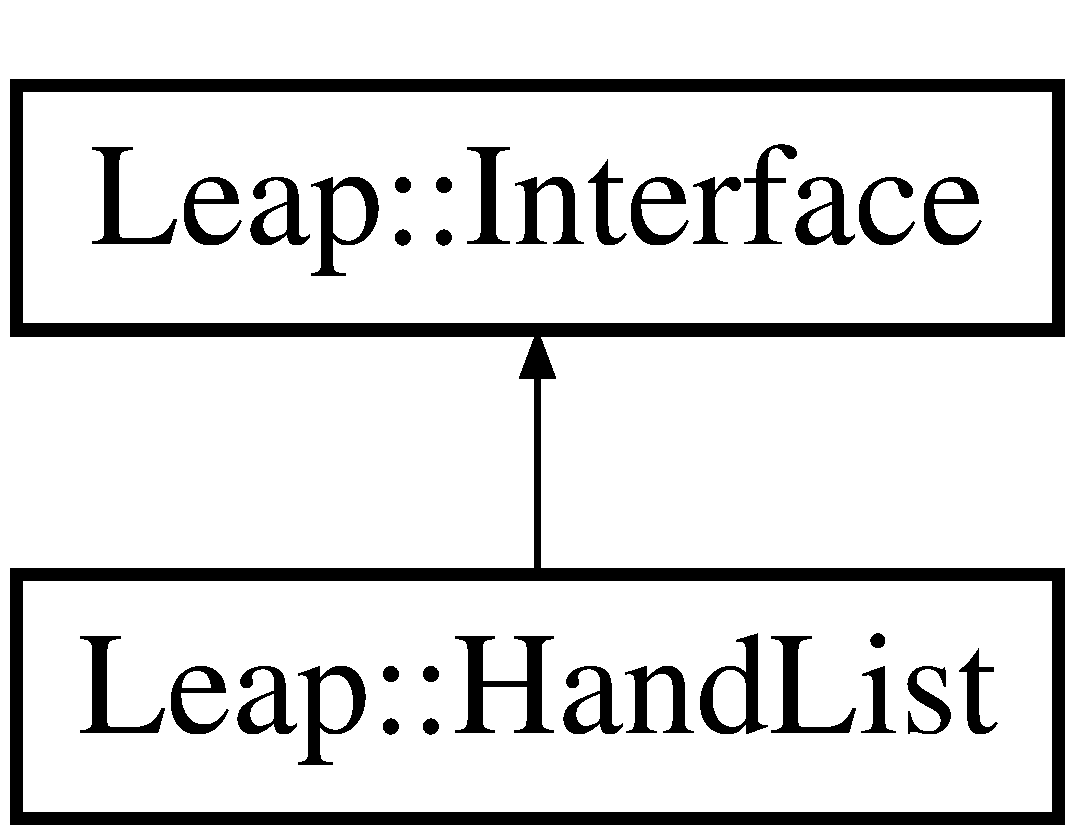
\includegraphics[height=2.000000cm]{class_leap_1_1_hand_list}
\end{center}
\end{figure}
\subsection*{Public Types}
\begin{DoxyCompactItemize}
\item 
typedef \hyperlink{class_leap_1_1_const_list_iterator}{Const\+List\+Iterator}\\*
$<$ \hyperlink{class_leap_1_1_hand_list}{Hand\+List}, \hyperlink{class_leap_1_1_hand}{Hand} $>$ \hyperlink{class_leap_1_1_hand_list_a9c35a4db8fd94a3b1a029efecbd13668}{const\+\_\+iterator}
\end{DoxyCompactItemize}
\subsection*{Public Member Functions}
\begin{DoxyCompactItemize}
\item 
\hypertarget{class_leap_1_1_hand_list_a5f0e45c94fcbb0e43395732142bd7bb1}{{\bfseries Hand\+List} (const \hyperlink{class_leap_1_1_list_base_implementation}{List\+Base\+Implementation}$<$ \hyperlink{class_leap_1_1_hand}{Hand} $>$ \&)}\label{class_leap_1_1_hand_list_a5f0e45c94fcbb0e43395732142bd7bb1}

\item 
L\+E\+A\+P\+\_\+\+E\+X\+P\+O\+R\+T \hyperlink{class_leap_1_1_hand_list_a98b159b1e306e8ae0da3d99ae1eba8d3}{Hand\+List} ()
\item 
L\+E\+A\+P\+\_\+\+E\+X\+P\+O\+R\+T int \hyperlink{class_leap_1_1_hand_list_a295c831f0f081b171c24b5c58cf7caf0}{count} () const 
\item 
L\+E\+A\+P\+\_\+\+E\+X\+P\+O\+R\+T bool \hyperlink{class_leap_1_1_hand_list_adb6551505d5ac31fa927a4b4d81108c5}{is\+Empty} () const 
\item 
L\+E\+A\+P\+\_\+\+E\+X\+P\+O\+R\+T \hyperlink{class_leap_1_1_hand}{Hand} \hyperlink{class_leap_1_1_hand_list_ad5831967b9e61cfe4abbeba476ca5462}{operator\mbox{[}$\,$\mbox{]}} (int index) const 
\item 
L\+E\+A\+P\+\_\+\+E\+X\+P\+O\+R\+T \hyperlink{class_leap_1_1_hand_list}{Hand\+List} \& \hyperlink{class_leap_1_1_hand_list_a7715a0e0df3e513c6cb1869691ef982d}{append} (const \hyperlink{class_leap_1_1_hand_list}{Hand\+List} \&other)
\item 
L\+E\+A\+P\+\_\+\+E\+X\+P\+O\+R\+T \hyperlink{class_leap_1_1_hand}{Hand} \hyperlink{class_leap_1_1_hand_list_a3ba586cd7485eeafde9d685753138b52}{leftmost} () const 
\item 
L\+E\+A\+P\+\_\+\+E\+X\+P\+O\+R\+T \hyperlink{class_leap_1_1_hand}{Hand} \hyperlink{class_leap_1_1_hand_list_a7123132de1d18b883a4344b38001ddc5}{rightmost} () const 
\item 
L\+E\+A\+P\+\_\+\+E\+X\+P\+O\+R\+T \hyperlink{class_leap_1_1_hand}{Hand} \hyperlink{class_leap_1_1_hand_list_ade694cc02f04254d32421d77d8bdc45c}{frontmost} () const 
\item 
L\+E\+A\+P\+\_\+\+E\+X\+P\+O\+R\+T \hyperlink{class_leap_1_1_hand_list_a9c35a4db8fd94a3b1a029efecbd13668}{const\+\_\+iterator} \hyperlink{class_leap_1_1_hand_list_ac3d04f28abd474e576df5c34a6c972e0}{begin} () const 
\item 
L\+E\+A\+P\+\_\+\+E\+X\+P\+O\+R\+T \hyperlink{class_leap_1_1_hand_list_a9c35a4db8fd94a3b1a029efecbd13668}{const\+\_\+iterator} \hyperlink{class_leap_1_1_hand_list_a227637f8beefa00d76745b30aac7c82f}{end} () const 
\end{DoxyCompactItemize}
\subsection*{Additional Inherited Members}


\subsection{Detailed Description}
The \hyperlink{class_leap_1_1_hand_list}{Hand\+List} class represents a list of \hyperlink{class_leap_1_1_hand}{Hand} objects.

Get a \hyperlink{class_leap_1_1_hand_list}{Hand\+List} object by calling \hyperlink{class_leap_1_1_frame_ab9e46956b8a90dafdce75803b4b6bdf8}{Frame\+::hands()}. \begin{DoxySince}{Since}
1.\+0 
\end{DoxySince}


\subsection{Member Typedef Documentation}
\hypertarget{class_leap_1_1_hand_list_a9c35a4db8fd94a3b1a029efecbd13668}{\index{Leap\+::\+Hand\+List@{Leap\+::\+Hand\+List}!const\+\_\+iterator@{const\+\_\+iterator}}
\index{const\+\_\+iterator@{const\+\_\+iterator}!Leap\+::\+Hand\+List@{Leap\+::\+Hand\+List}}
\subsubsection[{const\+\_\+iterator}]{\setlength{\rightskip}{0pt plus 5cm}typedef {\bf Const\+List\+Iterator}$<${\bf Hand\+List}, {\bf Hand}$>$ {\bf Leap\+::\+Hand\+List\+::const\+\_\+iterator}}}\label{class_leap_1_1_hand_list_a9c35a4db8fd94a3b1a029efecbd13668}
A C++ iterator type for this \hyperlink{class_leap_1_1_hand_list}{Hand\+List} objects. \begin{DoxySince}{Since}
1.\+0 
\end{DoxySince}


\subsection{Constructor \& Destructor Documentation}
\hypertarget{class_leap_1_1_hand_list_a98b159b1e306e8ae0da3d99ae1eba8d3}{\index{Leap\+::\+Hand\+List@{Leap\+::\+Hand\+List}!Hand\+List@{Hand\+List}}
\index{Hand\+List@{Hand\+List}!Leap\+::\+Hand\+List@{Leap\+::\+Hand\+List}}
\subsubsection[{Hand\+List}]{\setlength{\rightskip}{0pt plus 5cm}L\+E\+A\+P\+\_\+\+E\+X\+P\+O\+R\+T Leap\+::\+Hand\+List\+::\+Hand\+List (
\begin{DoxyParamCaption}
{}
\end{DoxyParamCaption}
)}}\label{class_leap_1_1_hand_list_a98b159b1e306e8ae0da3d99ae1eba8d3}
Constructs an empty list of hands. \begin{DoxySince}{Since}
1.\+0 
\end{DoxySince}


\subsection{Member Function Documentation}
\hypertarget{class_leap_1_1_hand_list_a7715a0e0df3e513c6cb1869691ef982d}{\index{Leap\+::\+Hand\+List@{Leap\+::\+Hand\+List}!append@{append}}
\index{append@{append}!Leap\+::\+Hand\+List@{Leap\+::\+Hand\+List}}
\subsubsection[{append}]{\setlength{\rightskip}{0pt plus 5cm}L\+E\+A\+P\+\_\+\+E\+X\+P\+O\+R\+T {\bf Hand\+List}\& Leap\+::\+Hand\+List\+::append (
\begin{DoxyParamCaption}
\item[{const {\bf Hand\+List} \&}]{other}
\end{DoxyParamCaption}
)}}\label{class_leap_1_1_hand_list_a7715a0e0df3e513c6cb1869691ef982d}
Appends the members of the specifed \hyperlink{class_leap_1_1_hand_list}{Hand\+List} to this \hyperlink{class_leap_1_1_hand_list}{Hand\+List}. 
\begin{DoxyParams}{Parameters}
{\em other} & A \hyperlink{class_leap_1_1_hand_list}{Hand\+List} object containing \hyperlink{class_leap_1_1_hand}{Hand} objects to append to the end of this \hyperlink{class_leap_1_1_hand_list}{Hand\+List}. \\
\hline
\end{DoxyParams}
\hypertarget{class_leap_1_1_hand_list_ac3d04f28abd474e576df5c34a6c972e0}{\index{Leap\+::\+Hand\+List@{Leap\+::\+Hand\+List}!begin@{begin}}
\index{begin@{begin}!Leap\+::\+Hand\+List@{Leap\+::\+Hand\+List}}
\subsubsection[{begin}]{\setlength{\rightskip}{0pt plus 5cm}L\+E\+A\+P\+\_\+\+E\+X\+P\+O\+R\+T {\bf const\+\_\+iterator} Leap\+::\+Hand\+List\+::begin (
\begin{DoxyParamCaption}
{}
\end{DoxyParamCaption}
) const}}\label{class_leap_1_1_hand_list_ac3d04f28abd474e576df5c34a6c972e0}
The C++ iterator set to the beginning of this \hyperlink{class_leap_1_1_hand_list}{Hand\+List}. \begin{DoxySince}{Since}
1.\+0 
\end{DoxySince}
\hypertarget{class_leap_1_1_hand_list_a295c831f0f081b171c24b5c58cf7caf0}{\index{Leap\+::\+Hand\+List@{Leap\+::\+Hand\+List}!count@{count}}
\index{count@{count}!Leap\+::\+Hand\+List@{Leap\+::\+Hand\+List}}
\subsubsection[{count}]{\setlength{\rightskip}{0pt plus 5cm}L\+E\+A\+P\+\_\+\+E\+X\+P\+O\+R\+T int Leap\+::\+Hand\+List\+::count (
\begin{DoxyParamCaption}
{}
\end{DoxyParamCaption}
) const}}\label{class_leap_1_1_hand_list_a295c831f0f081b171c24b5c58cf7caf0}
Returns the number of hands in this list. \begin{DoxyReturn}{Returns}
The number of hands in this list. 
\end{DoxyReturn}
\begin{DoxySince}{Since}
1.\+0 
\end{DoxySince}
\hypertarget{class_leap_1_1_hand_list_a227637f8beefa00d76745b30aac7c82f}{\index{Leap\+::\+Hand\+List@{Leap\+::\+Hand\+List}!end@{end}}
\index{end@{end}!Leap\+::\+Hand\+List@{Leap\+::\+Hand\+List}}
\subsubsection[{end}]{\setlength{\rightskip}{0pt plus 5cm}L\+E\+A\+P\+\_\+\+E\+X\+P\+O\+R\+T {\bf const\+\_\+iterator} Leap\+::\+Hand\+List\+::end (
\begin{DoxyParamCaption}
{}
\end{DoxyParamCaption}
) const}}\label{class_leap_1_1_hand_list_a227637f8beefa00d76745b30aac7c82f}
The C++ iterator set to the end of this \hyperlink{class_leap_1_1_hand_list}{Hand\+List}. \begin{DoxySince}{Since}
1.\+0 
\end{DoxySince}
\hypertarget{class_leap_1_1_hand_list_ade694cc02f04254d32421d77d8bdc45c}{\index{Leap\+::\+Hand\+List@{Leap\+::\+Hand\+List}!frontmost@{frontmost}}
\index{frontmost@{frontmost}!Leap\+::\+Hand\+List@{Leap\+::\+Hand\+List}}
\subsubsection[{frontmost}]{\setlength{\rightskip}{0pt plus 5cm}L\+E\+A\+P\+\_\+\+E\+X\+P\+O\+R\+T {\bf Hand} Leap\+::\+Hand\+List\+::frontmost (
\begin{DoxyParamCaption}
{}
\end{DoxyParamCaption}
) const}}\label{class_leap_1_1_hand_list_ade694cc02f04254d32421d77d8bdc45c}
The member of the list that is farthest to the front within the standard Leap Motion frame of reference (i.\+e has the smallest Z coordinate).

\begin{DoxyReturn}{Returns}
The frontmost hand, or invalid if list is empty. 
\end{DoxyReturn}
\begin{DoxySince}{Since}
1.\+0 
\end{DoxySince}
\hypertarget{class_leap_1_1_hand_list_adb6551505d5ac31fa927a4b4d81108c5}{\index{Leap\+::\+Hand\+List@{Leap\+::\+Hand\+List}!is\+Empty@{is\+Empty}}
\index{is\+Empty@{is\+Empty}!Leap\+::\+Hand\+List@{Leap\+::\+Hand\+List}}
\subsubsection[{is\+Empty}]{\setlength{\rightskip}{0pt plus 5cm}L\+E\+A\+P\+\_\+\+E\+X\+P\+O\+R\+T bool Leap\+::\+Hand\+List\+::is\+Empty (
\begin{DoxyParamCaption}
{}
\end{DoxyParamCaption}
) const}}\label{class_leap_1_1_hand_list_adb6551505d5ac31fa927a4b4d81108c5}
Reports whether the list is empty. \begin{DoxyReturn}{Returns}
True, if the list has no members. 
\end{DoxyReturn}
\begin{DoxySince}{Since}
1.\+0 
\end{DoxySince}
\hypertarget{class_leap_1_1_hand_list_a3ba586cd7485eeafde9d685753138b52}{\index{Leap\+::\+Hand\+List@{Leap\+::\+Hand\+List}!leftmost@{leftmost}}
\index{leftmost@{leftmost}!Leap\+::\+Hand\+List@{Leap\+::\+Hand\+List}}
\subsubsection[{leftmost}]{\setlength{\rightskip}{0pt plus 5cm}L\+E\+A\+P\+\_\+\+E\+X\+P\+O\+R\+T {\bf Hand} Leap\+::\+Hand\+List\+::leftmost (
\begin{DoxyParamCaption}
{}
\end{DoxyParamCaption}
) const}}\label{class_leap_1_1_hand_list_a3ba586cd7485eeafde9d685753138b52}
The member of the list that is farthest to the left within the standard Leap Motion frame of reference (i.\+e has the smallest X coordinate).

\begin{DoxyReturn}{Returns}
The leftmost hand, or invalid if list is empty. 
\end{DoxyReturn}
\begin{DoxySince}{Since}
1.\+0 
\end{DoxySince}
\hypertarget{class_leap_1_1_hand_list_ad5831967b9e61cfe4abbeba476ca5462}{\index{Leap\+::\+Hand\+List@{Leap\+::\+Hand\+List}!operator\mbox{[}$\,$\mbox{]}@{operator[]}}
\index{operator\mbox{[}$\,$\mbox{]}@{operator[]}!Leap\+::\+Hand\+List@{Leap\+::\+Hand\+List}}
\subsubsection[{operator[]}]{\setlength{\rightskip}{0pt plus 5cm}L\+E\+A\+P\+\_\+\+E\+X\+P\+O\+R\+T {\bf Hand} Leap\+::\+Hand\+List\+::operator\mbox{[}$\,$\mbox{]} (
\begin{DoxyParamCaption}
\item[{int}]{index}
\end{DoxyParamCaption}
) const}}\label{class_leap_1_1_hand_list_ad5831967b9e61cfe4abbeba476ca5462}
Access a list member by its position in the list. 
\begin{DoxyParams}{Parameters}
{\em index} & The zero-\/based list position index. \\
\hline
\end{DoxyParams}
\begin{DoxyReturn}{Returns}
The \hyperlink{class_leap_1_1_hand}{Hand} object at the specified index. 
\end{DoxyReturn}
\begin{DoxySince}{Since}
1.\+0 
\end{DoxySince}
\hypertarget{class_leap_1_1_hand_list_a7123132de1d18b883a4344b38001ddc5}{\index{Leap\+::\+Hand\+List@{Leap\+::\+Hand\+List}!rightmost@{rightmost}}
\index{rightmost@{rightmost}!Leap\+::\+Hand\+List@{Leap\+::\+Hand\+List}}
\subsubsection[{rightmost}]{\setlength{\rightskip}{0pt plus 5cm}L\+E\+A\+P\+\_\+\+E\+X\+P\+O\+R\+T {\bf Hand} Leap\+::\+Hand\+List\+::rightmost (
\begin{DoxyParamCaption}
{}
\end{DoxyParamCaption}
) const}}\label{class_leap_1_1_hand_list_a7123132de1d18b883a4344b38001ddc5}
The member of the list that is farthest to the right within the standard Leap Motion frame of reference (i.\+e has the largest X coordinate).

\begin{DoxyReturn}{Returns}
The rightmost hand, or invalid if list is empty. 
\end{DoxyReturn}
\begin{DoxySince}{Since}
1.\+0 
\end{DoxySince}


The documentation for this class was generated from the following file\+:\begin{DoxyCompactItemize}
\item 
Interface\+Managers/Leap.\+h\end{DoxyCompactItemize}

\hypertarget{struct_leap_1_1_interface_1_1_implementation}{\section{Leap\+:\+:Interface\+:\+:Implementation Struct Reference}
\label{struct_leap_1_1_interface_1_1_implementation}\index{Leap\+::\+Interface\+::\+Implementation@{Leap\+::\+Interface\+::\+Implementation}}
}


The documentation for this struct was generated from the following file\+:\begin{DoxyCompactItemize}
\item 
Interface\+Managers/Leap.\+h\end{DoxyCompactItemize}

\hypertarget{class_input_manager}{\section{Input\+Manager Class Reference}
\label{class_input_manager}\index{Input\+Manager@{Input\+Manager}}
}


{\ttfamily \#include $<$inputmanager.\+h$>$}

Inheritance diagram for Input\+Manager\+:\begin{figure}[H]
\begin{center}
\leavevmode
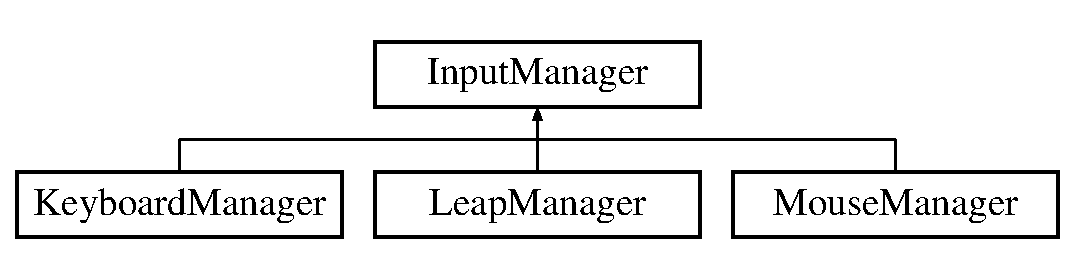
\includegraphics[height=2.000000cm]{class_input_manager}
\end{center}
\end{figure}
\subsection*{Public Member Functions}
\begin{DoxyCompactItemize}
\item 
virtual \hyperlink{class_input_manager_adf6f0d9103512c1bd7d89c54ddd299fe}{$\sim$\+Input\+Manager} ()
\item 
virtual void \hyperlink{class_input_manager_a9e689d7906407b5c0de0d384d457dbd6}{add\+Observer} (Event\+Listener $\ast$observer)
\item 
virtual void \hyperlink{class_input_manager_a35582c7c194fb8af1c649556e4935d08}{remove\+Observer} (Event\+Listener $\ast$observer)
\end{DoxyCompactItemize}
\subsection*{Protected Member Functions}
\begin{DoxyCompactItemize}
\item 
virtual void \hyperlink{class_input_manager_a4040fa67ecc810c5da6110ecf42b8bc7}{notify\+Observers} (Quadrant\+I\+D q, Event\+Type e)
\end{DoxyCompactItemize}


\subsection{Detailed Description}
An abstract class for input devices 

\subsection{Constructor \& Destructor Documentation}
\hypertarget{class_input_manager_adf6f0d9103512c1bd7d89c54ddd299fe}{\index{Input\+Manager@{Input\+Manager}!````~Input\+Manager@{$\sim$\+Input\+Manager}}
\index{````~Input\+Manager@{$\sim$\+Input\+Manager}!Input\+Manager@{Input\+Manager}}
\subsubsection[{$\sim$\+Input\+Manager}]{\setlength{\rightskip}{0pt plus 5cm}virtual Input\+Manager\+::$\sim$\+Input\+Manager (
\begin{DoxyParamCaption}
{}
\end{DoxyParamCaption}
)\hspace{0.3cm}{\ttfamily [inline]}, {\ttfamily [virtual]}}}\label{class_input_manager_adf6f0d9103512c1bd7d89c54ddd299fe}
Virtual destructor 

\subsection{Member Function Documentation}
\hypertarget{class_input_manager_a9e689d7906407b5c0de0d384d457dbd6}{\index{Input\+Manager@{Input\+Manager}!add\+Observer@{add\+Observer}}
\index{add\+Observer@{add\+Observer}!Input\+Manager@{Input\+Manager}}
\subsubsection[{add\+Observer}]{\setlength{\rightskip}{0pt plus 5cm}void Input\+Manager\+::add\+Observer (
\begin{DoxyParamCaption}
\item[{Event\+Listener $\ast$}]{observer}
\end{DoxyParamCaption}
)\hspace{0.3cm}{\ttfamily [virtual]}}}\label{class_input_manager_a9e689d7906407b5c0de0d384d457dbd6}
Add an Event\+Listener as an observer \hypertarget{class_input_manager_a4040fa67ecc810c5da6110ecf42b8bc7}{\index{Input\+Manager@{Input\+Manager}!notify\+Observers@{notify\+Observers}}
\index{notify\+Observers@{notify\+Observers}!Input\+Manager@{Input\+Manager}}
\subsubsection[{notify\+Observers}]{\setlength{\rightskip}{0pt plus 5cm}void Input\+Manager\+::notify\+Observers (
\begin{DoxyParamCaption}
\item[{Quadrant\+I\+D}]{q, }
\item[{Event\+Type}]{e}
\end{DoxyParamCaption}
)\hspace{0.3cm}{\ttfamily [protected]}, {\ttfamily [virtual]}}}\label{class_input_manager_a4040fa67ecc810c5da6110ecf42b8bc7}
Notify all observers of an event \hypertarget{class_input_manager_a35582c7c194fb8af1c649556e4935d08}{\index{Input\+Manager@{Input\+Manager}!remove\+Observer@{remove\+Observer}}
\index{remove\+Observer@{remove\+Observer}!Input\+Manager@{Input\+Manager}}
\subsubsection[{remove\+Observer}]{\setlength{\rightskip}{0pt plus 5cm}void Input\+Manager\+::remove\+Observer (
\begin{DoxyParamCaption}
\item[{Event\+Listener $\ast$}]{observer}
\end{DoxyParamCaption}
)\hspace{0.3cm}{\ttfamily [virtual]}}}\label{class_input_manager_a35582c7c194fb8af1c649556e4935d08}
Remove an Event\+Listener as an observer 

The documentation for this class was generated from the following files\+:\begin{DoxyCompactItemize}
\item 
Interface\+Managers/inputmanager.\+h\item 
Interface\+Managers/inputmanager.\+cpp\end{DoxyCompactItemize}

\hypertarget{class_leap_1_1_interaction_box}{\section{Leap\+:\+:Interaction\+Box Class Reference}
\label{class_leap_1_1_interaction_box}\index{Leap\+::\+Interaction\+Box@{Leap\+::\+Interaction\+Box}}
}


{\ttfamily \#include $<$Leap.\+h$>$}

Inheritance diagram for Leap\+:\+:Interaction\+Box\+:\begin{figure}[H]
\begin{center}
\leavevmode
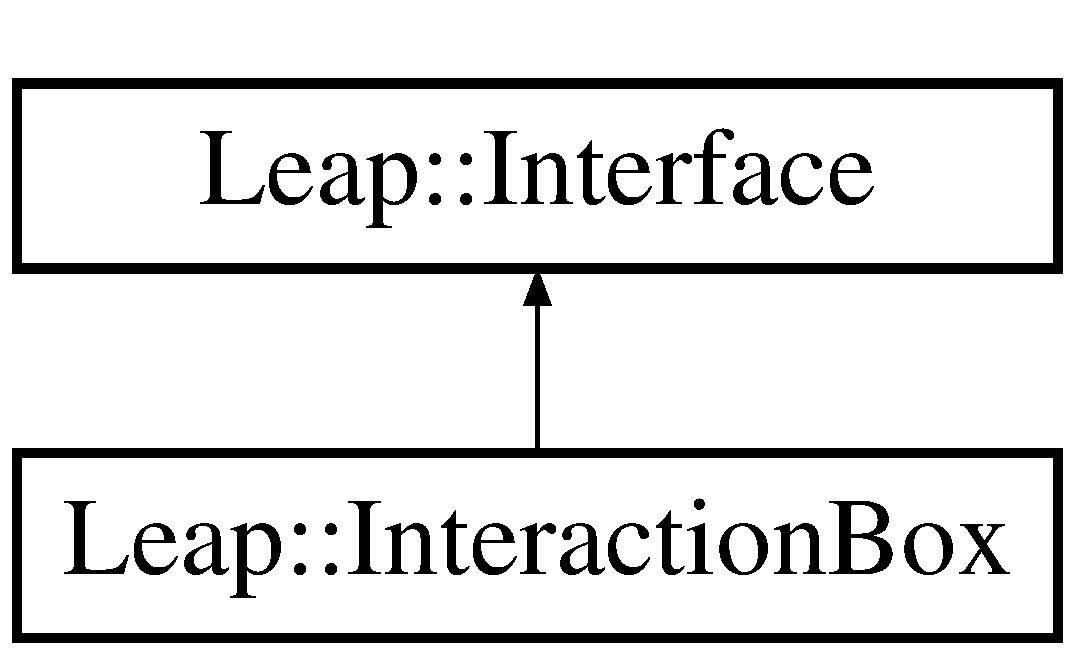
\includegraphics[height=2.000000cm]{class_leap_1_1_interaction_box}
\end{center}
\end{figure}
\subsection*{Public Member Functions}
\begin{DoxyCompactItemize}
\item 
\hypertarget{class_leap_1_1_interaction_box_a4762a10792e968f9d8fb02c8a79d6597}{{\bfseries Interaction\+Box} (Interaction\+Box\+Implementation $\ast$)}\label{class_leap_1_1_interaction_box_a4762a10792e968f9d8fb02c8a79d6597}

\item 
L\+E\+A\+P\+\_\+\+E\+X\+P\+O\+R\+T \hyperlink{struct_leap_1_1_vector}{Vector} \hyperlink{class_leap_1_1_interaction_box_a66ff2e3d02ae3d54ec1b93223c7b9ece}{normalize\+Point} (const \hyperlink{struct_leap_1_1_vector}{Vector} \&position, bool clamp=true) const 
\item 
L\+E\+A\+P\+\_\+\+E\+X\+P\+O\+R\+T \hyperlink{struct_leap_1_1_vector}{Vector} \hyperlink{class_leap_1_1_interaction_box_aa53fc603462adb3008bf7ed795029adb}{denormalize\+Point} (const \hyperlink{struct_leap_1_1_vector}{Vector} \&normalized\+Position) const 
\item 
L\+E\+A\+P\+\_\+\+E\+X\+P\+O\+R\+T \hyperlink{struct_leap_1_1_vector}{Vector} \hyperlink{class_leap_1_1_interaction_box_a674a8aa6308b32b1c85b2d39ee55875d}{center} () const 
\item 
L\+E\+A\+P\+\_\+\+E\+X\+P\+O\+R\+T float \hyperlink{class_leap_1_1_interaction_box_ab373a1adbabe141c0171f3dfa03085f3}{width} () const 
\item 
L\+E\+A\+P\+\_\+\+E\+X\+P\+O\+R\+T float \hyperlink{class_leap_1_1_interaction_box_afdde2aec9590e627e6a16a443ec4f4b7}{height} () const 
\item 
L\+E\+A\+P\+\_\+\+E\+X\+P\+O\+R\+T float \hyperlink{class_leap_1_1_interaction_box_afc9c1a582acba924f97504661ab2cbe3}{depth} () const 
\item 
L\+E\+A\+P\+\_\+\+E\+X\+P\+O\+R\+T bool \hyperlink{class_leap_1_1_interaction_box_a3c2a351d3fc38aebdc630fdb5a6cb846}{is\+Valid} () const 
\item 
L\+E\+A\+P\+\_\+\+E\+X\+P\+O\+R\+T bool \hyperlink{class_leap_1_1_interaction_box_a8d574045866dc11f571efc26cb93347a}{operator==} (const \hyperlink{class_leap_1_1_interaction_box}{Interaction\+Box} \&) const 
\item 
L\+E\+A\+P\+\_\+\+E\+X\+P\+O\+R\+T bool \hyperlink{class_leap_1_1_interaction_box_a1614fb599e63a9639d2ba54dbcf6f3d2}{operator!=} (const \hyperlink{class_leap_1_1_interaction_box}{Interaction\+Box} \&) const 
\item 
L\+E\+A\+P\+\_\+\+E\+X\+P\+O\+R\+T std\+::string \hyperlink{class_leap_1_1_interaction_box_abcd2e64f3ada1678c1de02db9dbba368}{to\+String} () const 
\end{DoxyCompactItemize}
\subsection*{Static Public Member Functions}
\begin{DoxyCompactItemize}
\item 
static L\+E\+A\+P\+\_\+\+E\+X\+P\+O\+R\+T const \\*
\hyperlink{class_leap_1_1_interaction_box}{Interaction\+Box} \& \hyperlink{class_leap_1_1_interaction_box_af3d181a4077f0b7e7334e3eb4db4b019}{invalid} ()
\end{DoxyCompactItemize}
\subsection*{Friends}
\begin{DoxyCompactItemize}
\item 
L\+E\+A\+P\+\_\+\+E\+X\+P\+O\+R\+T friend std\+::ostream \& \hyperlink{class_leap_1_1_interaction_box_a35cb230346cbaebc7c2a7dca7917c89e}{operator$<$$<$} (std\+::ostream \&, const \hyperlink{class_leap_1_1_interaction_box}{Interaction\+Box} \&)
\end{DoxyCompactItemize}
\subsection*{Additional Inherited Members}


\subsection{Detailed Description}
The \hyperlink{class_leap_1_1_interaction_box}{Interaction\+Box} class represents a box-\/shaped region completely within the field of view of the Leap Motion controller.

The interaction box is an axis-\/aligned rectangular prism and provides normalized coordinates for hands, fingers, and tools within this box. The \hyperlink{class_leap_1_1_interaction_box}{Interaction\+Box} class can make it easier to map positions in the Leap Motion coordinate system to 2\+D or 3\+D coordinate systems used for application drawing.



The \hyperlink{class_leap_1_1_interaction_box}{Interaction\+Box} region is defined by a center and dimensions along the x, y, and z axes.

Get an \hyperlink{class_leap_1_1_interaction_box}{Interaction\+Box} object from a \hyperlink{class_leap_1_1_frame}{Frame} object. \begin{DoxySince}{Since}
1.\+0 
\end{DoxySince}


\subsection{Member Function Documentation}
\hypertarget{class_leap_1_1_interaction_box_a674a8aa6308b32b1c85b2d39ee55875d}{\index{Leap\+::\+Interaction\+Box@{Leap\+::\+Interaction\+Box}!center@{center}}
\index{center@{center}!Leap\+::\+Interaction\+Box@{Leap\+::\+Interaction\+Box}}
\subsubsection[{center}]{\setlength{\rightskip}{0pt plus 5cm}L\+E\+A\+P\+\_\+\+E\+X\+P\+O\+R\+T {\bf Vector} Leap\+::\+Interaction\+Box\+::center (
\begin{DoxyParamCaption}
{}
\end{DoxyParamCaption}
) const}}\label{class_leap_1_1_interaction_box_a674a8aa6308b32b1c85b2d39ee55875d}
The center of the \hyperlink{class_leap_1_1_interaction_box}{Interaction\+Box} in device coordinates (millimeters). This point is equidistant from all sides of the box.

\begin{DoxyReturn}{Returns}
The \hyperlink{class_leap_1_1_interaction_box}{Interaction\+Box} center in device coordinates. 
\end{DoxyReturn}
\begin{DoxySince}{Since}
1.\+0 
\end{DoxySince}
\hypertarget{class_leap_1_1_interaction_box_aa53fc603462adb3008bf7ed795029adb}{\index{Leap\+::\+Interaction\+Box@{Leap\+::\+Interaction\+Box}!denormalize\+Point@{denormalize\+Point}}
\index{denormalize\+Point@{denormalize\+Point}!Leap\+::\+Interaction\+Box@{Leap\+::\+Interaction\+Box}}
\subsubsection[{denormalize\+Point}]{\setlength{\rightskip}{0pt plus 5cm}L\+E\+A\+P\+\_\+\+E\+X\+P\+O\+R\+T {\bf Vector} Leap\+::\+Interaction\+Box\+::denormalize\+Point (
\begin{DoxyParamCaption}
\item[{const {\bf Vector} \&}]{normalized\+Position}
\end{DoxyParamCaption}
) const}}\label{class_leap_1_1_interaction_box_aa53fc603462adb3008bf7ed795029adb}
Converts a position defined by normalized \hyperlink{class_leap_1_1_interaction_box}{Interaction\+Box} coordinates into device coordinates in millimeters.

This function performs the inverse of \hyperlink{class_leap_1_1_interaction_box_a66ff2e3d02ae3d54ec1b93223c7b9ece}{normalize\+Point()}.


\begin{DoxyParams}{Parameters}
{\em normalized\+Position} & The input position in \hyperlink{class_leap_1_1_interaction_box}{Interaction\+Box} coordinates. \\
\hline
\end{DoxyParams}
\begin{DoxyReturn}{Returns}
The corresponding denormalized position in device coordinates. 
\end{DoxyReturn}
\begin{DoxySince}{Since}
1.\+0 
\end{DoxySince}
\hypertarget{class_leap_1_1_interaction_box_afc9c1a582acba924f97504661ab2cbe3}{\index{Leap\+::\+Interaction\+Box@{Leap\+::\+Interaction\+Box}!depth@{depth}}
\index{depth@{depth}!Leap\+::\+Interaction\+Box@{Leap\+::\+Interaction\+Box}}
\subsubsection[{depth}]{\setlength{\rightskip}{0pt plus 5cm}L\+E\+A\+P\+\_\+\+E\+X\+P\+O\+R\+T float Leap\+::\+Interaction\+Box\+::depth (
\begin{DoxyParamCaption}
{}
\end{DoxyParamCaption}
) const}}\label{class_leap_1_1_interaction_box_afc9c1a582acba924f97504661ab2cbe3}
The depth of the \hyperlink{class_leap_1_1_interaction_box}{Interaction\+Box} in millimeters, measured along the z-\/axis.

\begin{DoxyReturn}{Returns}
The \hyperlink{class_leap_1_1_interaction_box}{Interaction\+Box} depth in millimeters. 
\end{DoxyReturn}
\begin{DoxySince}{Since}
1.\+0 
\end{DoxySince}
\hypertarget{class_leap_1_1_interaction_box_afdde2aec9590e627e6a16a443ec4f4b7}{\index{Leap\+::\+Interaction\+Box@{Leap\+::\+Interaction\+Box}!height@{height}}
\index{height@{height}!Leap\+::\+Interaction\+Box@{Leap\+::\+Interaction\+Box}}
\subsubsection[{height}]{\setlength{\rightskip}{0pt plus 5cm}L\+E\+A\+P\+\_\+\+E\+X\+P\+O\+R\+T float Leap\+::\+Interaction\+Box\+::height (
\begin{DoxyParamCaption}
{}
\end{DoxyParamCaption}
) const}}\label{class_leap_1_1_interaction_box_afdde2aec9590e627e6a16a443ec4f4b7}
The height of the \hyperlink{class_leap_1_1_interaction_box}{Interaction\+Box} in millimeters, measured along the y-\/axis.

\begin{DoxyReturn}{Returns}
The \hyperlink{class_leap_1_1_interaction_box}{Interaction\+Box} height in millimeters. 
\end{DoxyReturn}
\begin{DoxySince}{Since}
1.\+0 
\end{DoxySince}
\hypertarget{class_leap_1_1_interaction_box_af3d181a4077f0b7e7334e3eb4db4b019}{\index{Leap\+::\+Interaction\+Box@{Leap\+::\+Interaction\+Box}!invalid@{invalid}}
\index{invalid@{invalid}!Leap\+::\+Interaction\+Box@{Leap\+::\+Interaction\+Box}}
\subsubsection[{invalid}]{\setlength{\rightskip}{0pt plus 5cm}static L\+E\+A\+P\+\_\+\+E\+X\+P\+O\+R\+T const {\bf Interaction\+Box}\& Leap\+::\+Interaction\+Box\+::invalid (
\begin{DoxyParamCaption}
{}
\end{DoxyParamCaption}
)\hspace{0.3cm}{\ttfamily [static]}}}\label{class_leap_1_1_interaction_box_af3d181a4077f0b7e7334e3eb4db4b019}
Returns an invalid \hyperlink{class_leap_1_1_interaction_box}{Interaction\+Box} object.

You can use the instance returned by this function in comparisons testing whether a given \hyperlink{class_leap_1_1_interaction_box}{Interaction\+Box} instance is valid or invalid. (You can also use the \hyperlink{class_leap_1_1_interaction_box_a3c2a351d3fc38aebdc630fdb5a6cb846}{Interaction\+Box\+::is\+Valid()} function.)

\begin{DoxyReturn}{Returns}
The invalid \hyperlink{class_leap_1_1_interaction_box}{Interaction\+Box} instance. 
\end{DoxyReturn}
\begin{DoxySince}{Since}
1.\+0 
\end{DoxySince}
\hypertarget{class_leap_1_1_interaction_box_a3c2a351d3fc38aebdc630fdb5a6cb846}{\index{Leap\+::\+Interaction\+Box@{Leap\+::\+Interaction\+Box}!is\+Valid@{is\+Valid}}
\index{is\+Valid@{is\+Valid}!Leap\+::\+Interaction\+Box@{Leap\+::\+Interaction\+Box}}
\subsubsection[{is\+Valid}]{\setlength{\rightskip}{0pt plus 5cm}L\+E\+A\+P\+\_\+\+E\+X\+P\+O\+R\+T bool Leap\+::\+Interaction\+Box\+::is\+Valid (
\begin{DoxyParamCaption}
{}
\end{DoxyParamCaption}
) const}}\label{class_leap_1_1_interaction_box_a3c2a351d3fc38aebdc630fdb5a6cb846}
Reports whether this is a valid \hyperlink{class_leap_1_1_interaction_box}{Interaction\+Box} object.

\begin{DoxyReturn}{Returns}
True, if this \hyperlink{class_leap_1_1_interaction_box}{Interaction\+Box} object contains valid data. 
\end{DoxyReturn}
\begin{DoxySince}{Since}
1.\+0 
\end{DoxySince}
\hypertarget{class_leap_1_1_interaction_box_a66ff2e3d02ae3d54ec1b93223c7b9ece}{\index{Leap\+::\+Interaction\+Box@{Leap\+::\+Interaction\+Box}!normalize\+Point@{normalize\+Point}}
\index{normalize\+Point@{normalize\+Point}!Leap\+::\+Interaction\+Box@{Leap\+::\+Interaction\+Box}}
\subsubsection[{normalize\+Point}]{\setlength{\rightskip}{0pt plus 5cm}L\+E\+A\+P\+\_\+\+E\+X\+P\+O\+R\+T {\bf Vector} Leap\+::\+Interaction\+Box\+::normalize\+Point (
\begin{DoxyParamCaption}
\item[{const {\bf Vector} \&}]{position, }
\item[{bool}]{clamp = {\ttfamily true}}
\end{DoxyParamCaption}
) const}}\label{class_leap_1_1_interaction_box_a66ff2e3d02ae3d54ec1b93223c7b9ece}
Normalizes the coordinates of a point using the interaction box.

Coordinates from the Leap Motion frame of reference (millimeters) are converted to a range of \mbox{[}0..1\mbox{]} such that the minimum value of the \hyperlink{class_leap_1_1_interaction_box}{Interaction\+Box} maps to 0 and the maximum value of the \hyperlink{class_leap_1_1_interaction_box}{Interaction\+Box} maps to 1.


\begin{DoxyParams}{Parameters}
{\em position} & The input position in device coordinates. \\
\hline
{\em clamp} & Whether or not to limit the output value to the range \mbox{[}0,1\mbox{]} when the input position is outside the \hyperlink{class_leap_1_1_interaction_box}{Interaction\+Box}. Defaults to true. \\
\hline
\end{DoxyParams}
\begin{DoxyReturn}{Returns}
The normalized position. 
\end{DoxyReturn}
\begin{DoxySince}{Since}
1.\+0 
\end{DoxySince}
\hypertarget{class_leap_1_1_interaction_box_a1614fb599e63a9639d2ba54dbcf6f3d2}{\index{Leap\+::\+Interaction\+Box@{Leap\+::\+Interaction\+Box}!operator"!=@{operator"!=}}
\index{operator"!=@{operator"!=}!Leap\+::\+Interaction\+Box@{Leap\+::\+Interaction\+Box}}
\subsubsection[{operator"!=}]{\setlength{\rightskip}{0pt plus 5cm}L\+E\+A\+P\+\_\+\+E\+X\+P\+O\+R\+T bool Leap\+::\+Interaction\+Box\+::operator!= (
\begin{DoxyParamCaption}
\item[{const {\bf Interaction\+Box} \&}]{}
\end{DoxyParamCaption}
) const}}\label{class_leap_1_1_interaction_box_a1614fb599e63a9639d2ba54dbcf6f3d2}
Compare \hyperlink{class_leap_1_1_interaction_box}{Interaction\+Box} object inequality. Two \hyperlink{class_leap_1_1_interaction_box}{Interaction\+Box} objects are equal if and only if both \hyperlink{class_leap_1_1_interaction_box}{Interaction\+Box} objects represent the exact same \hyperlink{class_leap_1_1_interaction_box}{Interaction\+Box} and both Interaction\+Boxes are valid. \begin{DoxySince}{Since}
1.\+0 
\end{DoxySince}
\hypertarget{class_leap_1_1_interaction_box_a8d574045866dc11f571efc26cb93347a}{\index{Leap\+::\+Interaction\+Box@{Leap\+::\+Interaction\+Box}!operator==@{operator==}}
\index{operator==@{operator==}!Leap\+::\+Interaction\+Box@{Leap\+::\+Interaction\+Box}}
\subsubsection[{operator==}]{\setlength{\rightskip}{0pt plus 5cm}L\+E\+A\+P\+\_\+\+E\+X\+P\+O\+R\+T bool Leap\+::\+Interaction\+Box\+::operator== (
\begin{DoxyParamCaption}
\item[{const {\bf Interaction\+Box} \&}]{}
\end{DoxyParamCaption}
) const}}\label{class_leap_1_1_interaction_box_a8d574045866dc11f571efc26cb93347a}
Compare \hyperlink{class_leap_1_1_interaction_box}{Interaction\+Box} object equality. Two \hyperlink{class_leap_1_1_interaction_box}{Interaction\+Box} objects are equal if and only if both \hyperlink{class_leap_1_1_interaction_box}{Interaction\+Box} objects represent the exact same \hyperlink{class_leap_1_1_interaction_box}{Interaction\+Box} and both Interaction\+Boxes are valid. \begin{DoxySince}{Since}
1.\+0 
\end{DoxySince}
\hypertarget{class_leap_1_1_interaction_box_abcd2e64f3ada1678c1de02db9dbba368}{\index{Leap\+::\+Interaction\+Box@{Leap\+::\+Interaction\+Box}!to\+String@{to\+String}}
\index{to\+String@{to\+String}!Leap\+::\+Interaction\+Box@{Leap\+::\+Interaction\+Box}}
\subsubsection[{to\+String}]{\setlength{\rightskip}{0pt plus 5cm}L\+E\+A\+P\+\_\+\+E\+X\+P\+O\+R\+T std\+::string Leap\+::\+Interaction\+Box\+::to\+String (
\begin{DoxyParamCaption}
{}
\end{DoxyParamCaption}
) const}}\label{class_leap_1_1_interaction_box_abcd2e64f3ada1678c1de02db9dbba368}
A string containing a brief, human readable description of the \hyperlink{class_leap_1_1_interaction_box}{Interaction\+Box} object.

\begin{DoxyReturn}{Returns}
A description of the \hyperlink{class_leap_1_1_interaction_box}{Interaction\+Box} as a string. 
\end{DoxyReturn}
\begin{DoxySince}{Since}
1.\+0 
\end{DoxySince}
\hypertarget{class_leap_1_1_interaction_box_ab373a1adbabe141c0171f3dfa03085f3}{\index{Leap\+::\+Interaction\+Box@{Leap\+::\+Interaction\+Box}!width@{width}}
\index{width@{width}!Leap\+::\+Interaction\+Box@{Leap\+::\+Interaction\+Box}}
\subsubsection[{width}]{\setlength{\rightskip}{0pt plus 5cm}L\+E\+A\+P\+\_\+\+E\+X\+P\+O\+R\+T float Leap\+::\+Interaction\+Box\+::width (
\begin{DoxyParamCaption}
{}
\end{DoxyParamCaption}
) const}}\label{class_leap_1_1_interaction_box_ab373a1adbabe141c0171f3dfa03085f3}
The width of the \hyperlink{class_leap_1_1_interaction_box}{Interaction\+Box} in millimeters, measured along the x-\/axis.

\begin{DoxyReturn}{Returns}
The \hyperlink{class_leap_1_1_interaction_box}{Interaction\+Box} width in millimeters. 
\end{DoxyReturn}
\begin{DoxySince}{Since}
1.\+0 
\end{DoxySince}


\subsection{Friends And Related Function Documentation}
\hypertarget{class_leap_1_1_interaction_box_a35cb230346cbaebc7c2a7dca7917c89e}{\index{Leap\+::\+Interaction\+Box@{Leap\+::\+Interaction\+Box}!operator$<$$<$@{operator$<$$<$}}
\index{operator$<$$<$@{operator$<$$<$}!Leap\+::\+Interaction\+Box@{Leap\+::\+Interaction\+Box}}
\subsubsection[{operator$<$$<$}]{\setlength{\rightskip}{0pt plus 5cm}L\+E\+A\+P\+\_\+\+E\+X\+P\+O\+R\+T friend std\+::ostream\& operator$<$$<$ (
\begin{DoxyParamCaption}
\item[{std\+::ostream \&}]{, }
\item[{const {\bf Interaction\+Box} \&}]{}
\end{DoxyParamCaption}
)\hspace{0.3cm}{\ttfamily [friend]}}}\label{class_leap_1_1_interaction_box_a35cb230346cbaebc7c2a7dca7917c89e}
Writes a brief, human readable description of the \hyperlink{class_leap_1_1_interaction_box}{Interaction\+Box} object. \begin{DoxySince}{Since}
1.\+0 
\end{DoxySince}


The documentation for this class was generated from the following file\+:\begin{DoxyCompactItemize}
\item 
Interface\+Managers/Leap.\+h\end{DoxyCompactItemize}

\hypertarget{class_leap_1_1_interface}{\section{Leap\+:\+:Interface Class Reference}
\label{class_leap_1_1_interface}\index{Leap\+::\+Interface@{Leap\+::\+Interface}}
}
Inheritance diagram for Leap\+:\+:Interface\+:\begin{figure}[H]
\begin{center}
\leavevmode
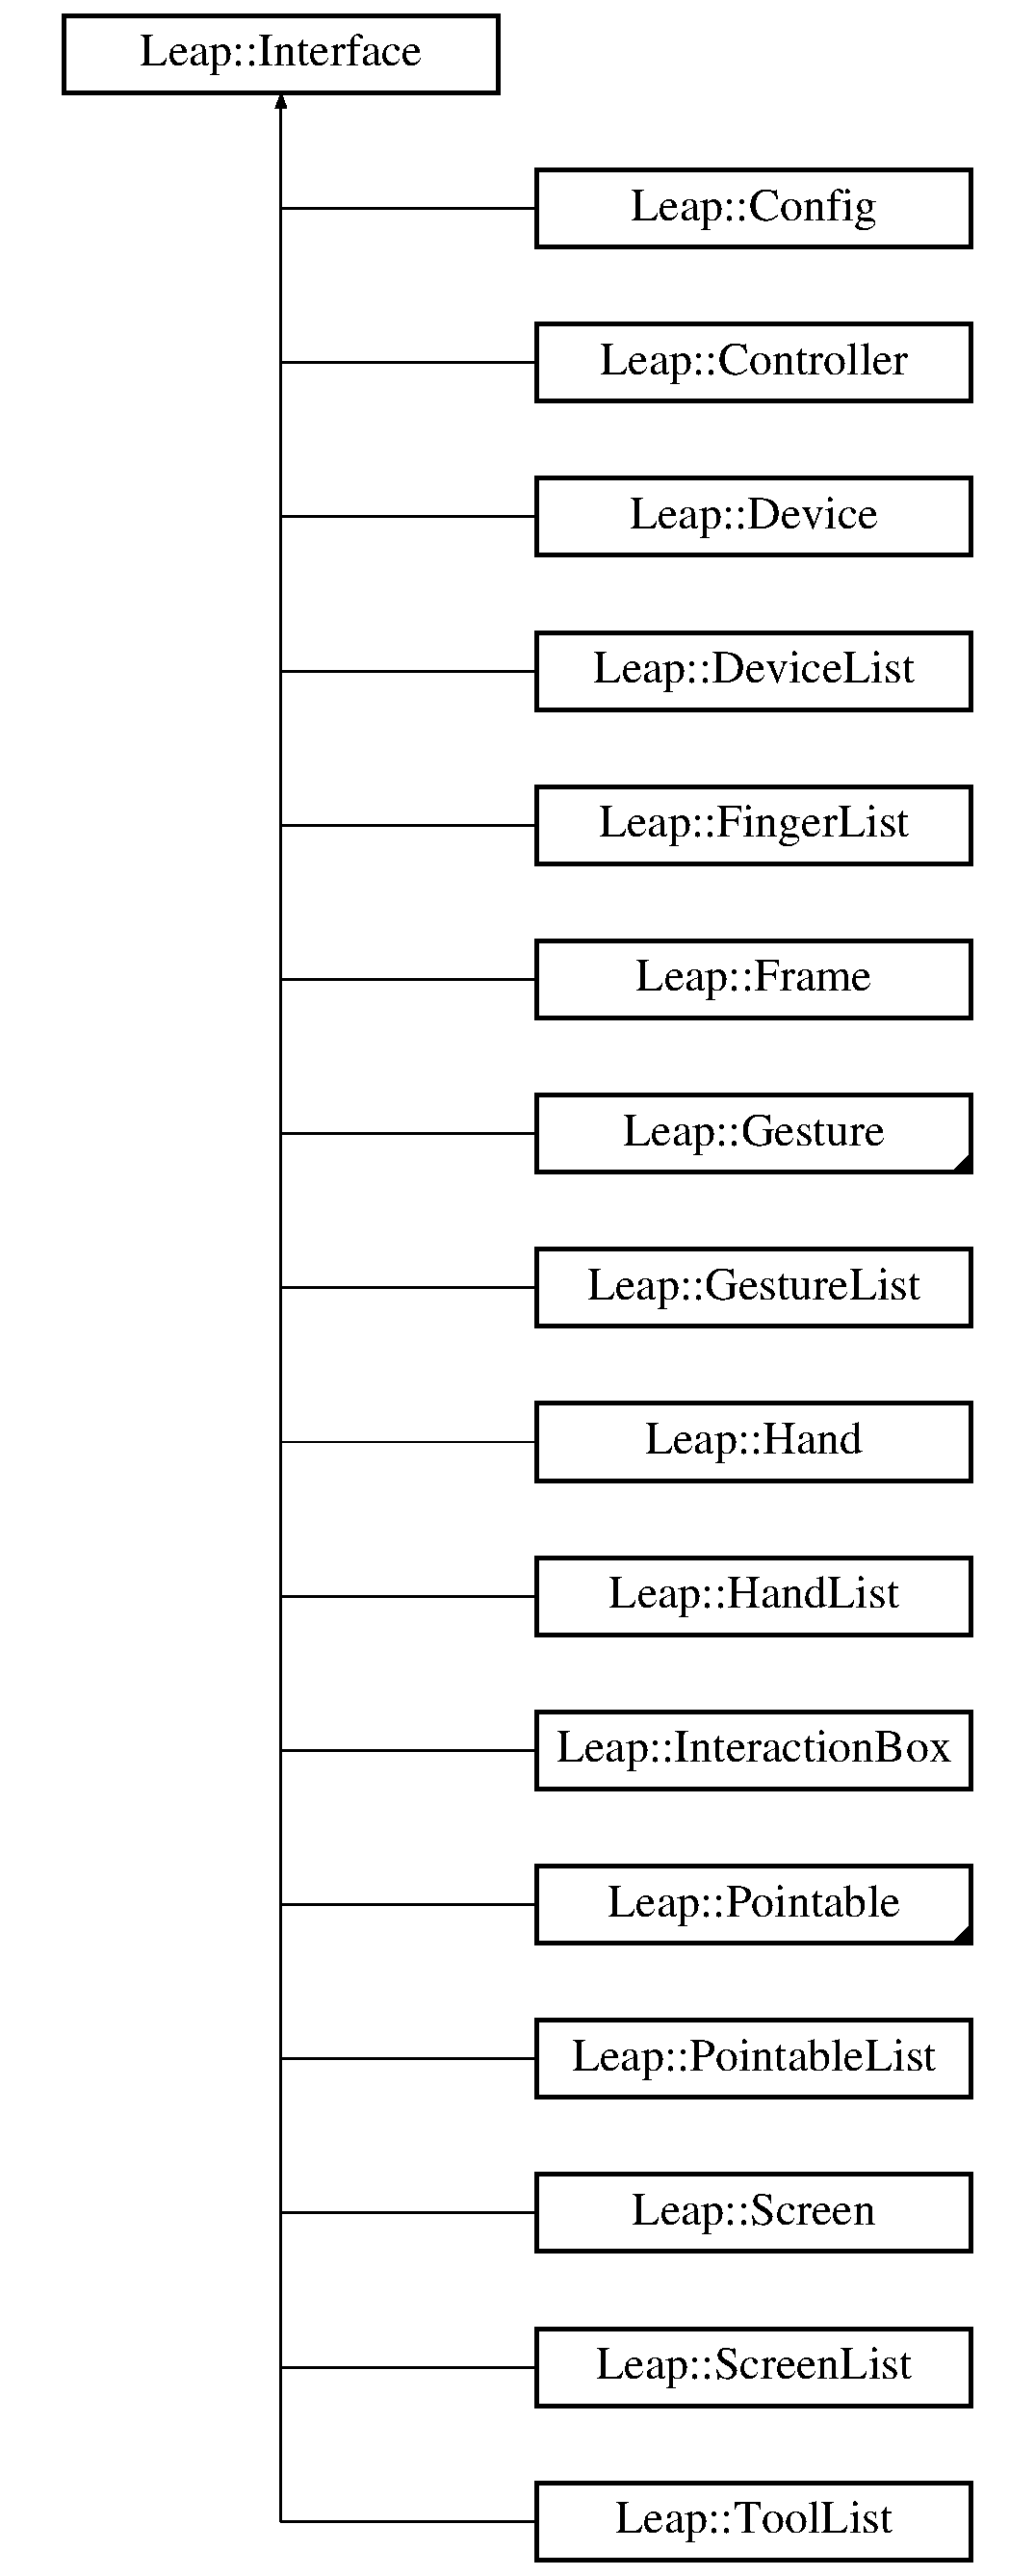
\includegraphics[height=12.000000cm]{class_leap_1_1_interface}
\end{center}
\end{figure}
\subsection*{Classes}
\begin{DoxyCompactItemize}
\item 
struct \hyperlink{struct_leap_1_1_interface_1_1_implementation}{Implementation}
\end{DoxyCompactItemize}
\subsection*{Protected Member Functions}
\begin{DoxyCompactItemize}
\item 
\hypertarget{class_leap_1_1_interface_ac3a173f44d98821f915ae5a873c478dc}{L\+E\+A\+P\+\_\+\+E\+X\+P\+O\+R\+T {\bfseries Interface} (void $\ast$owner)}\label{class_leap_1_1_interface_ac3a173f44d98821f915ae5a873c478dc}

\item 
\hypertarget{class_leap_1_1_interface_a0e76882987c7866e17856c699b2490a8}{L\+E\+A\+P\+\_\+\+E\+X\+P\+O\+R\+T {\bfseries Interface} (\hyperlink{struct_leap_1_1_interface_1_1_implementation}{Implementation} $\ast$reference, void $\ast$owner)}\label{class_leap_1_1_interface_a0e76882987c7866e17856c699b2490a8}

\item 
\hypertarget{class_leap_1_1_interface_a540323027de8d874d86f4ad09f5b7103}{L\+E\+A\+P\+\_\+\+E\+X\+P\+O\+R\+T {\bfseries Interface} (const \hyperlink{class_leap_1_1_interface}{Interface} \&rhs)}\label{class_leap_1_1_interface_a540323027de8d874d86f4ad09f5b7103}

\item 
\hypertarget{class_leap_1_1_interface_a48b7660b77d962b30fa397919901967b}{{\bfseries Interface} (class Shared\+Object $\ast$object)}\label{class_leap_1_1_interface_a48b7660b77d962b30fa397919901967b}

\item 
\hypertarget{class_leap_1_1_interface_a763c07d957f412613423acf2c9830275}{L\+E\+A\+P\+\_\+\+E\+X\+P\+O\+R\+T \hyperlink{class_leap_1_1_interface}{Interface} \& {\bfseries operator=} (const \hyperlink{class_leap_1_1_interface}{Interface} \&rhs)}\label{class_leap_1_1_interface_a763c07d957f412613423acf2c9830275}

\item 
\hypertarget{class_leap_1_1_interface_af5e59f158a1738b37b64d5161fad550a}{{\footnotesize template$<$typename T $>$ }\\T $\ast$ {\bfseries get} () const }\label{class_leap_1_1_interface_af5e59f158a1738b37b64d5161fad550a}

\end{DoxyCompactItemize}
\subsection*{Protected Attributes}
\begin{DoxyCompactItemize}
\item 
\hypertarget{class_leap_1_1_interface_aebf4e096301998b829239acd895b387c}{class Shared\+Object $\ast$ {\bfseries m\+\_\+object}}\label{class_leap_1_1_interface_aebf4e096301998b829239acd895b387c}

\end{DoxyCompactItemize}


The documentation for this class was generated from the following file\+:\begin{DoxyCompactItemize}
\item 
Interface\+Managers/Leap.\+h\end{DoxyCompactItemize}

\hypertarget{class_keyboard_manager}{\section{Keyboard\+Manager Class Reference}
\label{class_keyboard_manager}\index{Keyboard\+Manager@{Keyboard\+Manager}}
}


{\ttfamily \#include $<$keyboardmanager.\+h$>$}

Inheritance diagram for Keyboard\+Manager\+:\begin{figure}[H]
\begin{center}
\leavevmode
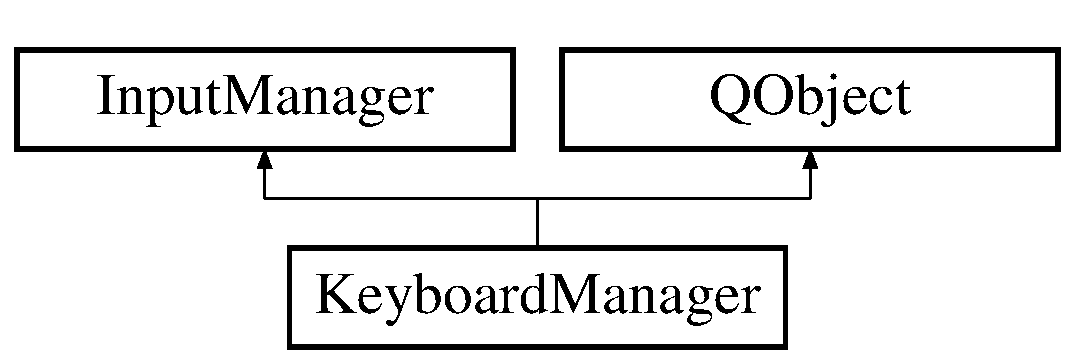
\includegraphics[height=2.000000cm]{class_keyboard_manager}
\end{center}
\end{figure}
\subsection*{Public Member Functions}
\begin{DoxyCompactItemize}
\item 
\hyperlink{class_keyboard_manager_a0aaf2801dbf2337111a5221b9acd6078}{Keyboard\+Manager} ()
\item 
\hyperlink{class_keyboard_manager_a5321f1327f94403ead6b7fa083ae7cee}{$\sim$\+Keyboard\+Manager} ()
\item 
bool \hyperlink{class_keyboard_manager_ae5934173dd590f5df2050afda354118e}{event\+Filter} (Q\+Object $\ast$, Q\+Event $\ast$event)
\end{DoxyCompactItemize}
\subsection*{Additional Inherited Members}


\subsection{Detailed Description}
A keyboard listener class 

\subsection{Constructor \& Destructor Documentation}
\hypertarget{class_keyboard_manager_a0aaf2801dbf2337111a5221b9acd6078}{\index{Keyboard\+Manager@{Keyboard\+Manager}!Keyboard\+Manager@{Keyboard\+Manager}}
\index{Keyboard\+Manager@{Keyboard\+Manager}!Keyboard\+Manager@{Keyboard\+Manager}}
\subsubsection[{Keyboard\+Manager}]{\setlength{\rightskip}{0pt plus 5cm}Keyboard\+Manager\+::\+Keyboard\+Manager (
\begin{DoxyParamCaption}
{}
\end{DoxyParamCaption}
)}}\label{class_keyboard_manager_a0aaf2801dbf2337111a5221b9acd6078}
Constructor \hypertarget{class_keyboard_manager_a5321f1327f94403ead6b7fa083ae7cee}{\index{Keyboard\+Manager@{Keyboard\+Manager}!````~Keyboard\+Manager@{$\sim$\+Keyboard\+Manager}}
\index{````~Keyboard\+Manager@{$\sim$\+Keyboard\+Manager}!Keyboard\+Manager@{Keyboard\+Manager}}
\subsubsection[{$\sim$\+Keyboard\+Manager}]{\setlength{\rightskip}{0pt plus 5cm}Keyboard\+Manager\+::$\sim$\+Keyboard\+Manager (
\begin{DoxyParamCaption}
{}
\end{DoxyParamCaption}
)}}\label{class_keyboard_manager_a5321f1327f94403ead6b7fa083ae7cee}
Destructor 

\subsection{Member Function Documentation}
\hypertarget{class_keyboard_manager_ae5934173dd590f5df2050afda354118e}{\index{Keyboard\+Manager@{Keyboard\+Manager}!event\+Filter@{event\+Filter}}
\index{event\+Filter@{event\+Filter}!Keyboard\+Manager@{Keyboard\+Manager}}
\subsubsection[{event\+Filter}]{\setlength{\rightskip}{0pt plus 5cm}bool Keyboard\+Manager\+::event\+Filter (
\begin{DoxyParamCaption}
\item[{Q\+Object $\ast$}]{, }
\item[{Q\+Event $\ast$}]{event}
\end{DoxyParamCaption}
)}}\label{class_keyboard_manager_ae5934173dd590f5df2050afda354118e}
Called when an event occurs on the main ui 

The documentation for this class was generated from the following files\+:\begin{DoxyCompactItemize}
\item 
Interface\+Managers/keyboardmanager.\+h\item 
Interface\+Managers/keyboardmanager.\+cpp\end{DoxyCompactItemize}

\hypertarget{class_leap_1_1_key_tap_gesture}{\section{Leap\+:\+:Key\+Tap\+Gesture Class Reference}
\label{class_leap_1_1_key_tap_gesture}\index{Leap\+::\+Key\+Tap\+Gesture@{Leap\+::\+Key\+Tap\+Gesture}}
}


{\ttfamily \#include $<$Leap.\+h$>$}

Inheritance diagram for Leap\+:\+:Key\+Tap\+Gesture\+:\begin{figure}[H]
\begin{center}
\leavevmode
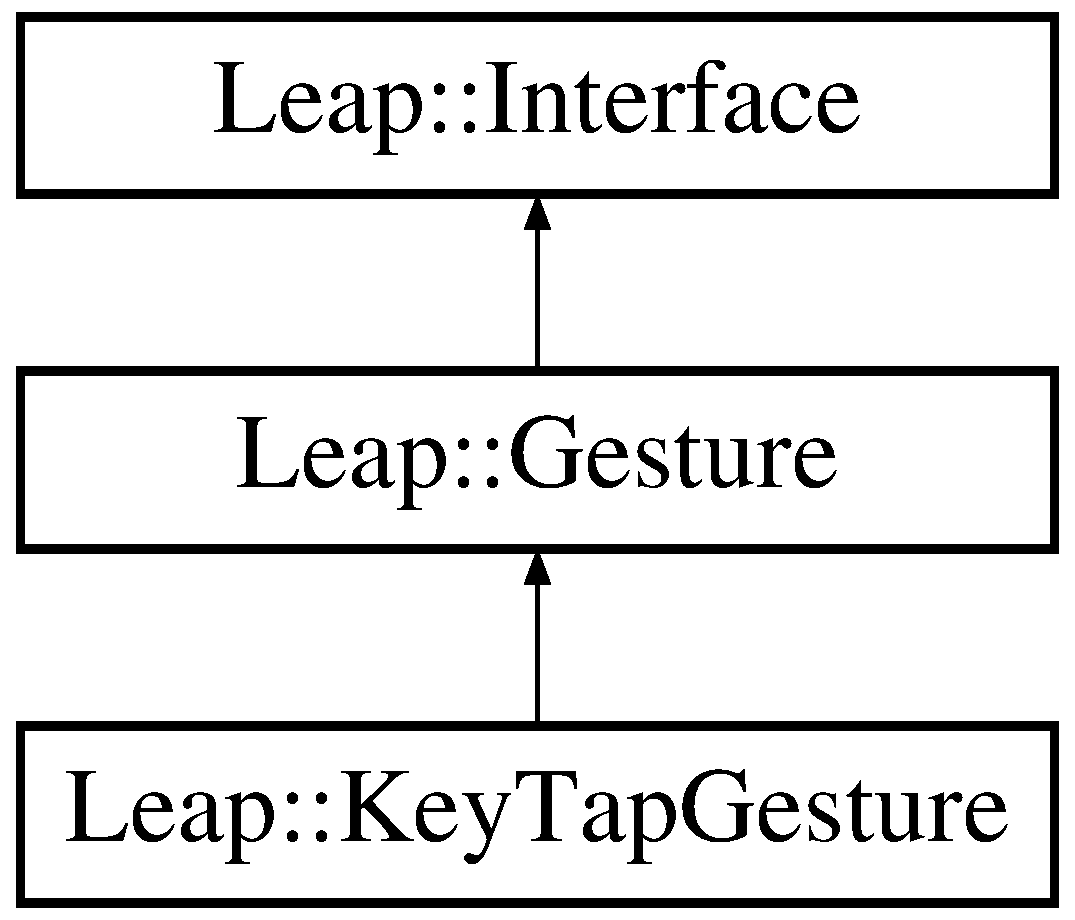
\includegraphics[height=3.000000cm]{class_leap_1_1_key_tap_gesture}
\end{center}
\end{figure}
\subsection*{Public Member Functions}
\begin{DoxyCompactItemize}
\item 
L\+E\+A\+P\+\_\+\+E\+X\+P\+O\+R\+T \hyperlink{class_leap_1_1_key_tap_gesture_a916eb2060586a29c499b0201cef9b203}{Key\+Tap\+Gesture} ()
\item 
L\+E\+A\+P\+\_\+\+E\+X\+P\+O\+R\+T \hyperlink{class_leap_1_1_key_tap_gesture_a701172268caa05b6c05bf3cd8578bde5}{Key\+Tap\+Gesture} (const \hyperlink{class_leap_1_1_gesture}{Gesture} \&rhs)
\item 
L\+E\+A\+P\+\_\+\+E\+X\+P\+O\+R\+T \hyperlink{struct_leap_1_1_vector}{Vector} \hyperlink{class_leap_1_1_key_tap_gesture_a2f9de1992ab50eeaa0cbfaa0499420bd}{position} () const 
\item 
L\+E\+A\+P\+\_\+\+E\+X\+P\+O\+R\+T \hyperlink{struct_leap_1_1_vector}{Vector} \hyperlink{class_leap_1_1_key_tap_gesture_ab8bad7448409ee1f69548a3351303125}{direction} () const 
\item 
L\+E\+A\+P\+\_\+\+E\+X\+P\+O\+R\+T float \hyperlink{class_leap_1_1_key_tap_gesture_a1bd7863f9c3b70b8312cf0946bbb1569}{progress} () const 
\item 
L\+E\+A\+P\+\_\+\+E\+X\+P\+O\+R\+T \hyperlink{class_leap_1_1_pointable}{Pointable} \hyperlink{class_leap_1_1_key_tap_gesture_a2f1392201385cb36a84e6a3ff4152305}{pointable} () const 
\end{DoxyCompactItemize}
\subsection*{Static Public Member Functions}
\begin{DoxyCompactItemize}
\item 
static \hyperlink{class_leap_1_1_gesture_a6fa6dd4f28c502f0d55abc6b71c6f9b1}{Type} \hyperlink{class_leap_1_1_key_tap_gesture_a674173890d1f8b1b2d2cee98245b65f2}{class\+Type} ()
\end{DoxyCompactItemize}
\subsection*{Additional Inherited Members}


\subsection{Detailed Description}
The \hyperlink{class_leap_1_1_key_tap_gesture}{Key\+Tap\+Gesture} class represents a tapping gesture by a finger or tool.

A key tap gesture is recognized when the tip of a finger rotates down toward the palm and then springs back to approximately the original postion, as if tapping. The tapping finger must pause briefly before beginning the tap.



{\bfseries Important\+:} To use key tap gestures in your application, you must enable recognition of the key tap gesture. You can enable recognition with\+:


\begin{DoxyCodeInclude}
\end{DoxyCodeInclude}


Key tap gestures are discrete. The \hyperlink{class_leap_1_1_key_tap_gesture}{Key\+Tap\+Gesture} object representing a tap always has the state, S\+T\+A\+T\+E\+\_\+\+S\+T\+O\+P. Only one \hyperlink{class_leap_1_1_key_tap_gesture}{Key\+Tap\+Gesture} object is created for each key tap gesture recognized.

You can set the minimum finger movement and velocity required for a movement to be recognized as a key tap as well as adjust the detection window for evaluating the movement using the config attribute of a connected \hyperlink{class_leap_1_1_controller}{Controller} object. Use the following configuration keys to configure key tap recognition\+:

\begin{TabularC}{4}
\hline
\rowcolor{lightgray}{\bf Key string }&{\bf Value type }&{\bf Default value }&{\bf Units  }\\\cline{1-4}
Gesture.\+Key\+Tap.\+Min\+Down\+Velocity &float &50 &mm/s \\\cline{1-4}
Gesture.\+Key\+Tap.\+History\+Seconds &float &0.\+1 &s \\\cline{1-4}
Gesture.\+Key\+Tap.\+Min\+Distance &float &5.\+0 &mm \\\cline{1-4}
\end{TabularC}
The following example demonstrates how to set the key tap configuration parameters\+:


\begin{DoxyCodeInclude}
\end{DoxyCodeInclude}
 \begin{DoxySince}{Since}
1.\+0 
\end{DoxySince}


\subsection{Constructor \& Destructor Documentation}
\hypertarget{class_leap_1_1_key_tap_gesture_a916eb2060586a29c499b0201cef9b203}{\index{Leap\+::\+Key\+Tap\+Gesture@{Leap\+::\+Key\+Tap\+Gesture}!Key\+Tap\+Gesture@{Key\+Tap\+Gesture}}
\index{Key\+Tap\+Gesture@{Key\+Tap\+Gesture}!Leap\+::\+Key\+Tap\+Gesture@{Leap\+::\+Key\+Tap\+Gesture}}
\subsubsection[{Key\+Tap\+Gesture}]{\setlength{\rightskip}{0pt plus 5cm}L\+E\+A\+P\+\_\+\+E\+X\+P\+O\+R\+T Leap\+::\+Key\+Tap\+Gesture\+::\+Key\+Tap\+Gesture (
\begin{DoxyParamCaption}
{}
\end{DoxyParamCaption}
)}}\label{class_leap_1_1_key_tap_gesture_a916eb2060586a29c499b0201cef9b203}
Constructs a new \hyperlink{class_leap_1_1_key_tap_gesture}{Key\+Tap\+Gesture} object.

An uninitialized \hyperlink{class_leap_1_1_key_tap_gesture}{Key\+Tap\+Gesture} object is considered invalid. Get valid instances of the \hyperlink{class_leap_1_1_key_tap_gesture}{Key\+Tap\+Gesture} class from a \hyperlink{class_leap_1_1_frame}{Frame} object. \begin{DoxySince}{Since}
1.\+0 
\end{DoxySince}
\hypertarget{class_leap_1_1_key_tap_gesture_a701172268caa05b6c05bf3cd8578bde5}{\index{Leap\+::\+Key\+Tap\+Gesture@{Leap\+::\+Key\+Tap\+Gesture}!Key\+Tap\+Gesture@{Key\+Tap\+Gesture}}
\index{Key\+Tap\+Gesture@{Key\+Tap\+Gesture}!Leap\+::\+Key\+Tap\+Gesture@{Leap\+::\+Key\+Tap\+Gesture}}
\subsubsection[{Key\+Tap\+Gesture}]{\setlength{\rightskip}{0pt plus 5cm}L\+E\+A\+P\+\_\+\+E\+X\+P\+O\+R\+T Leap\+::\+Key\+Tap\+Gesture\+::\+Key\+Tap\+Gesture (
\begin{DoxyParamCaption}
\item[{const {\bf Gesture} \&}]{rhs}
\end{DoxyParamCaption}
)}}\label{class_leap_1_1_key_tap_gesture_a701172268caa05b6c05bf3cd8578bde5}
Constructs a \hyperlink{class_leap_1_1_key_tap_gesture}{Key\+Tap\+Gesture} object from an instance of the \hyperlink{class_leap_1_1_gesture}{Gesture} class.


\begin{DoxyParams}{Parameters}
{\em rhs} & The \hyperlink{class_leap_1_1_gesture}{Gesture} instance to specialize. This \hyperlink{class_leap_1_1_gesture}{Gesture} instance must be a \hyperlink{class_leap_1_1_key_tap_gesture}{Key\+Tap\+Gesture} object. \\
\hline
\end{DoxyParams}
\begin{DoxySince}{Since}
1.\+0 
\end{DoxySince}


\subsection{Member Function Documentation}
\hypertarget{class_leap_1_1_key_tap_gesture_a674173890d1f8b1b2d2cee98245b65f2}{\index{Leap\+::\+Key\+Tap\+Gesture@{Leap\+::\+Key\+Tap\+Gesture}!class\+Type@{class\+Type}}
\index{class\+Type@{class\+Type}!Leap\+::\+Key\+Tap\+Gesture@{Leap\+::\+Key\+Tap\+Gesture}}
\subsubsection[{class\+Type}]{\setlength{\rightskip}{0pt plus 5cm}static {\bf Type} Leap\+::\+Key\+Tap\+Gesture\+::class\+Type (
\begin{DoxyParamCaption}
{}
\end{DoxyParamCaption}
)\hspace{0.3cm}{\ttfamily [inline]}, {\ttfamily [static]}}}\label{class_leap_1_1_key_tap_gesture_a674173890d1f8b1b2d2cee98245b65f2}
The key tap gesture type.

\begin{DoxyReturn}{Returns}
Type The type value designating a key tap gesture. 
\end{DoxyReturn}
\begin{DoxySince}{Since}
1.\+0 
\end{DoxySince}
\hypertarget{class_leap_1_1_key_tap_gesture_ab8bad7448409ee1f69548a3351303125}{\index{Leap\+::\+Key\+Tap\+Gesture@{Leap\+::\+Key\+Tap\+Gesture}!direction@{direction}}
\index{direction@{direction}!Leap\+::\+Key\+Tap\+Gesture@{Leap\+::\+Key\+Tap\+Gesture}}
\subsubsection[{direction}]{\setlength{\rightskip}{0pt plus 5cm}L\+E\+A\+P\+\_\+\+E\+X\+P\+O\+R\+T {\bf Vector} Leap\+::\+Key\+Tap\+Gesture\+::direction (
\begin{DoxyParamCaption}
{}
\end{DoxyParamCaption}
) const}}\label{class_leap_1_1_key_tap_gesture_ab8bad7448409ee1f69548a3351303125}
The direction of finger tip motion.

\begin{DoxyReturn}{Returns}
\hyperlink{struct_leap_1_1_vector}{Vector} A unit direction vector if the finger tip is moving; otherwise, a zero-\/vector. 
\end{DoxyReturn}
\begin{DoxySince}{Since}
1.\+0 
\end{DoxySince}
\hypertarget{class_leap_1_1_key_tap_gesture_a2f1392201385cb36a84e6a3ff4152305}{\index{Leap\+::\+Key\+Tap\+Gesture@{Leap\+::\+Key\+Tap\+Gesture}!pointable@{pointable}}
\index{pointable@{pointable}!Leap\+::\+Key\+Tap\+Gesture@{Leap\+::\+Key\+Tap\+Gesture}}
\subsubsection[{pointable}]{\setlength{\rightskip}{0pt plus 5cm}L\+E\+A\+P\+\_\+\+E\+X\+P\+O\+R\+T {\bf Pointable} Leap\+::\+Key\+Tap\+Gesture\+::pointable (
\begin{DoxyParamCaption}
{}
\end{DoxyParamCaption}
) const}}\label{class_leap_1_1_key_tap_gesture_a2f1392201385cb36a84e6a3ff4152305}
The finger performing the key tap gesture.

\begin{DoxyReturn}{Returns}
\hyperlink{class_leap_1_1_pointable}{Pointable} A \hyperlink{class_leap_1_1_pointable}{Pointable} object representing the tapping finger. 
\end{DoxyReturn}
\begin{DoxySince}{Since}
1.\+0 
\end{DoxySince}
\hypertarget{class_leap_1_1_key_tap_gesture_a2f9de1992ab50eeaa0cbfaa0499420bd}{\index{Leap\+::\+Key\+Tap\+Gesture@{Leap\+::\+Key\+Tap\+Gesture}!position@{position}}
\index{position@{position}!Leap\+::\+Key\+Tap\+Gesture@{Leap\+::\+Key\+Tap\+Gesture}}
\subsubsection[{position}]{\setlength{\rightskip}{0pt plus 5cm}L\+E\+A\+P\+\_\+\+E\+X\+P\+O\+R\+T {\bf Vector} Leap\+::\+Key\+Tap\+Gesture\+::position (
\begin{DoxyParamCaption}
{}
\end{DoxyParamCaption}
) const}}\label{class_leap_1_1_key_tap_gesture_a2f9de1992ab50eeaa0cbfaa0499420bd}
The position where the key tap is registered.

\begin{DoxyReturn}{Returns}
\hyperlink{struct_leap_1_1_vector}{Vector} A \hyperlink{struct_leap_1_1_vector}{Vector} containing the coordinates of tap location. 
\end{DoxyReturn}
\begin{DoxySince}{Since}
1.\+0 
\end{DoxySince}
\hypertarget{class_leap_1_1_key_tap_gesture_a1bd7863f9c3b70b8312cf0946bbb1569}{\index{Leap\+::\+Key\+Tap\+Gesture@{Leap\+::\+Key\+Tap\+Gesture}!progress@{progress}}
\index{progress@{progress}!Leap\+::\+Key\+Tap\+Gesture@{Leap\+::\+Key\+Tap\+Gesture}}
\subsubsection[{progress}]{\setlength{\rightskip}{0pt plus 5cm}L\+E\+A\+P\+\_\+\+E\+X\+P\+O\+R\+T float Leap\+::\+Key\+Tap\+Gesture\+::progress (
\begin{DoxyParamCaption}
{}
\end{DoxyParamCaption}
) const}}\label{class_leap_1_1_key_tap_gesture_a1bd7863f9c3b70b8312cf0946bbb1569}
The progess value is always 1.\+0 for a key tap gesture.

\begin{DoxyReturn}{Returns}
float The value 1.\+0. 
\end{DoxyReturn}
\begin{DoxySince}{Since}
1.\+0 
\end{DoxySince}


The documentation for this class was generated from the following file\+:\begin{DoxyCompactItemize}
\item 
Interface\+Managers/Leap.\+h\end{DoxyCompactItemize}

\hypertarget{class_leap_manager}{\section{Leap\+Manager Class Reference}
\label{class_leap_manager}\index{Leap\+Manager@{Leap\+Manager}}
}


{\ttfamily \#include $<$leapmanager.\+h$>$}

Inheritance diagram for Leap\+Manager\+:\begin{figure}[H]
\begin{center}
\leavevmode
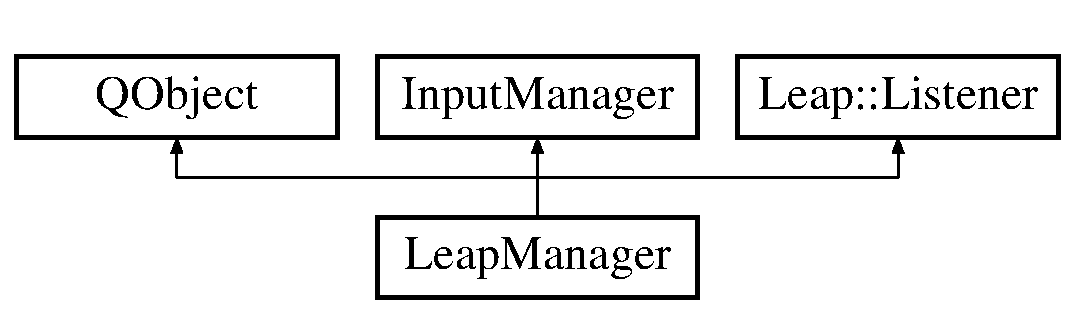
\includegraphics[height=2.000000cm]{class_leap_manager}
\end{center}
\end{figure}
\subsection*{Public Slots}
\begin{DoxyCompactItemize}
\item 
void \hyperlink{class_leap_manager_a5d50198b53659afa29f93ab38d6f730a}{notify\+On\+Main\+Queue} (int q, int e)
\end{DoxyCompactItemize}
\subsection*{Signals}
\begin{DoxyCompactItemize}
\item 
void \hyperlink{class_leap_manager_aaf97456260cb9f139ff7bf3771877b0a}{frame\+Finished} (int q, int e)
\end{DoxyCompactItemize}
\subsection*{Public Member Functions}
\begin{DoxyCompactItemize}
\item 
\hyperlink{class_leap_manager_a5b784234d2e338255e7a32c1cb40c535}{Leap\+Manager} ()
\item 
\hyperlink{class_leap_manager_ae6740e093904a960b0ac200e66596625}{$\sim$\+Leap\+Manager} ()
\item 
void \hyperlink{class_leap_manager_ad50649a573f5176b9bfcb4407ea7efd3}{on\+Frame} (const \hyperlink{class_leap_1_1_controller}{Leap\+::\+Controller} \&controller)
\end{DoxyCompactItemize}
\subsection*{Additional Inherited Members}


\subsection{Detailed Description}
Leap listener class for handling input from leap sensor 

\subsection{Constructor \& Destructor Documentation}
\hypertarget{class_leap_manager_a5b784234d2e338255e7a32c1cb40c535}{\index{Leap\+Manager@{Leap\+Manager}!Leap\+Manager@{Leap\+Manager}}
\index{Leap\+Manager@{Leap\+Manager}!Leap\+Manager@{Leap\+Manager}}
\subsubsection[{Leap\+Manager}]{\setlength{\rightskip}{0pt plus 5cm}Leap\+Manager\+::\+Leap\+Manager (
\begin{DoxyParamCaption}
{}
\end{DoxyParamCaption}
)}}\label{class_leap_manager_a5b784234d2e338255e7a32c1cb40c535}
Constructor -\/ sets up leap controller \hypertarget{class_leap_manager_ae6740e093904a960b0ac200e66596625}{\index{Leap\+Manager@{Leap\+Manager}!````~Leap\+Manager@{$\sim$\+Leap\+Manager}}
\index{````~Leap\+Manager@{$\sim$\+Leap\+Manager}!Leap\+Manager@{Leap\+Manager}}
\subsubsection[{$\sim$\+Leap\+Manager}]{\setlength{\rightskip}{0pt plus 5cm}Leap\+Manager\+::$\sim$\+Leap\+Manager (
\begin{DoxyParamCaption}
{}
\end{DoxyParamCaption}
)}}\label{class_leap_manager_ae6740e093904a960b0ac200e66596625}
Destructor -\/ removes as a listener 

\subsection{Member Function Documentation}
\hypertarget{class_leap_manager_aaf97456260cb9f139ff7bf3771877b0a}{\index{Leap\+Manager@{Leap\+Manager}!frame\+Finished@{frame\+Finished}}
\index{frame\+Finished@{frame\+Finished}!Leap\+Manager@{Leap\+Manager}}
\subsubsection[{frame\+Finished}]{\setlength{\rightskip}{0pt plus 5cm}void Leap\+Manager\+::frame\+Finished (
\begin{DoxyParamCaption}
\item[{int}]{q, }
\item[{int}]{e}
\end{DoxyParamCaption}
)\hspace{0.3cm}{\ttfamily [signal]}}}\label{class_leap_manager_aaf97456260cb9f139ff7bf3771877b0a}
Signal for when frame is done \hypertarget{class_leap_manager_a5d50198b53659afa29f93ab38d6f730a}{\index{Leap\+Manager@{Leap\+Manager}!notify\+On\+Main\+Queue@{notify\+On\+Main\+Queue}}
\index{notify\+On\+Main\+Queue@{notify\+On\+Main\+Queue}!Leap\+Manager@{Leap\+Manager}}
\subsubsection[{notify\+On\+Main\+Queue}]{\setlength{\rightskip}{0pt plus 5cm}void Leap\+Manager\+::notify\+On\+Main\+Queue (
\begin{DoxyParamCaption}
\item[{int}]{q, }
\item[{int}]{e}
\end{DoxyParamCaption}
)\hspace{0.3cm}{\ttfamily [slot]}}}\label{class_leap_manager_a5d50198b53659afa29f93ab38d6f730a}
Called on main thread after frame is processed \hypertarget{class_leap_manager_ad50649a573f5176b9bfcb4407ea7efd3}{\index{Leap\+Manager@{Leap\+Manager}!on\+Frame@{on\+Frame}}
\index{on\+Frame@{on\+Frame}!Leap\+Manager@{Leap\+Manager}}
\subsubsection[{on\+Frame}]{\setlength{\rightskip}{0pt plus 5cm}void Leap\+Manager\+::on\+Frame (
\begin{DoxyParamCaption}
\item[{const {\bf Leap\+::\+Controller} \&}]{controller}
\end{DoxyParamCaption}
)\hspace{0.3cm}{\ttfamily [virtual]}}}\label{class_leap_manager_ad50649a573f5176b9bfcb4407ea7efd3}
Called by the controller on each frame 

Reimplemented from \hyperlink{class_leap_1_1_listener_ab600421108bbc952d8f0f144384ca30f}{Leap\+::\+Listener}.



The documentation for this class was generated from the following files\+:\begin{DoxyCompactItemize}
\item 
Interface\+Managers/leapmanager.\+h\item 
Interface\+Managers/leapmanager.\+cpp\end{DoxyCompactItemize}

\hypertarget{class_leap_1_1_list_base_implementation}{\section{Leap\+:\+:List\+Base\+Implementation$<$ T $>$ Class Template Reference}
\label{class_leap_1_1_list_base_implementation}\index{Leap\+::\+List\+Base\+Implementation$<$ T $>$@{Leap\+::\+List\+Base\+Implementation$<$ T $>$}}
}


The documentation for this class was generated from the following file\+:\begin{DoxyCompactItemize}
\item 
Interface\+Managers/Leap.\+h\end{DoxyCompactItemize}

\hypertarget{class_leap_1_1_listener}{\section{Leap\+:\+:Listener Class Reference}
\label{class_leap_1_1_listener}\index{Leap\+::\+Listener@{Leap\+::\+Listener}}
}


{\ttfamily \#include $<$Leap.\+h$>$}

Inheritance diagram for Leap\+:\+:Listener\+:\begin{figure}[H]
\begin{center}
\leavevmode
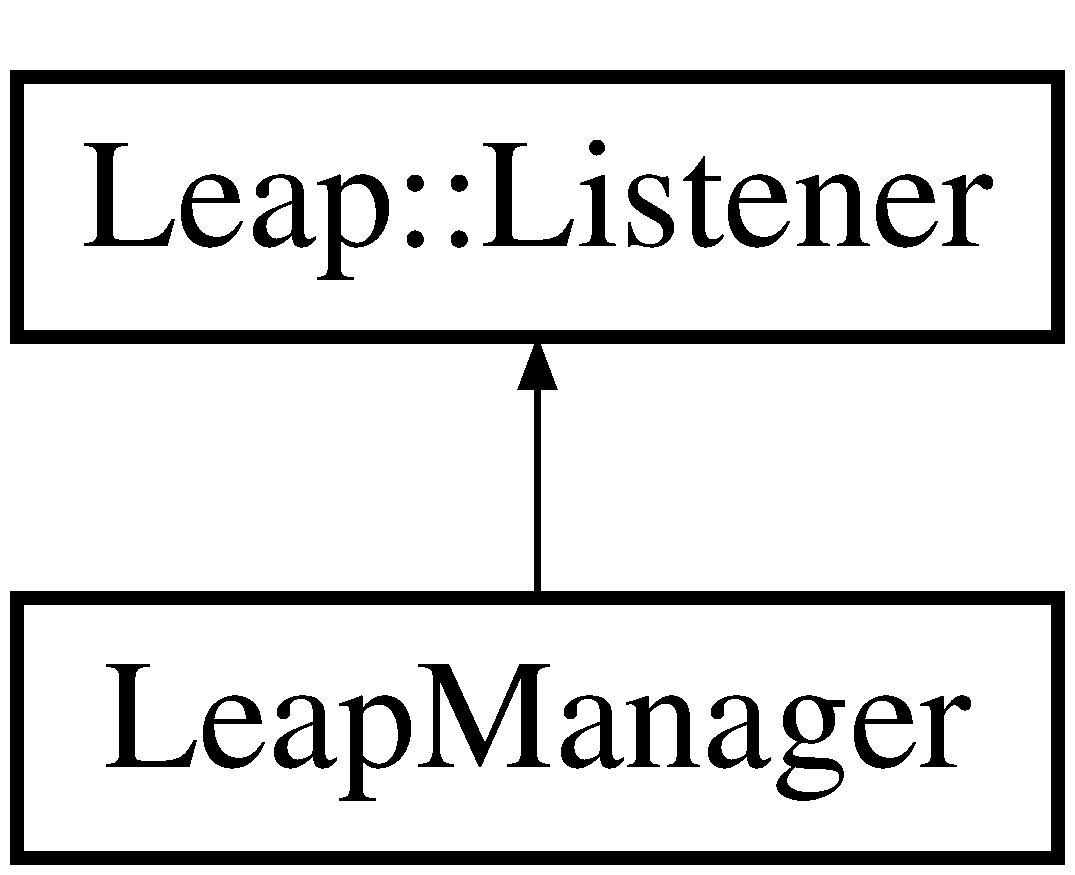
\includegraphics[height=2.000000cm]{class_leap_1_1_listener}
\end{center}
\end{figure}
\subsection*{Public Member Functions}
\begin{DoxyCompactItemize}
\item 
L\+E\+A\+P\+\_\+\+E\+X\+P\+O\+R\+T \hyperlink{class_leap_1_1_listener_a68f2cc4c80510c7f0bb47d1f576ffea9}{Listener} ()
\item 
virtual L\+E\+A\+P\+\_\+\+E\+X\+P\+O\+R\+T \hyperlink{class_leap_1_1_listener_a11a24ce72b609c45ec7010a3cb460d49}{$\sim$\+Listener} ()
\item 
virtual L\+E\+A\+P\+\_\+\+E\+X\+P\+O\+R\+T void \hyperlink{class_leap_1_1_listener_a180d621ad08afa5851d03d3546a82bbf}{on\+Init} (const \hyperlink{class_leap_1_1_controller}{Controller} \&)
\item 
virtual L\+E\+A\+P\+\_\+\+E\+X\+P\+O\+R\+T void \hyperlink{class_leap_1_1_listener_adfef79f9a03b342384aaa17f3a8ebf15}{on\+Connect} (const \hyperlink{class_leap_1_1_controller}{Controller} \&)
\item 
virtual L\+E\+A\+P\+\_\+\+E\+X\+P\+O\+R\+T void \hyperlink{class_leap_1_1_listener_ac031e2d95b530097e2060518a9190f5e}{on\+Disconnect} (const \hyperlink{class_leap_1_1_controller}{Controller} \&)
\item 
virtual L\+E\+A\+P\+\_\+\+E\+X\+P\+O\+R\+T void \hyperlink{class_leap_1_1_listener_ac8f779a9208101f0084953560923f88c}{on\+Exit} (const \hyperlink{class_leap_1_1_controller}{Controller} \&)
\item 
virtual L\+E\+A\+P\+\_\+\+E\+X\+P\+O\+R\+T void \hyperlink{class_leap_1_1_listener_ab600421108bbc952d8f0f144384ca30f}{on\+Frame} (const \hyperlink{class_leap_1_1_controller}{Controller} \&)
\item 
virtual L\+E\+A\+P\+\_\+\+E\+X\+P\+O\+R\+T void \hyperlink{class_leap_1_1_listener_ab52aa99ad9e8fd0f35d9dffc3ef9f027}{on\+Focus\+Gained} (const \hyperlink{class_leap_1_1_controller}{Controller} \&)
\item 
virtual L\+E\+A\+P\+\_\+\+E\+X\+P\+O\+R\+T void \hyperlink{class_leap_1_1_listener_a7bcae44a40674c3f1e367b911201d252}{on\+Focus\+Lost} (const \hyperlink{class_leap_1_1_controller}{Controller} \&)
\end{DoxyCompactItemize}


\subsection{Detailed Description}
The \hyperlink{class_leap_1_1_listener}{Listener} class defines a set of callback functions that you can override in a subclass to respond to events dispatched by the \hyperlink{class_leap_1_1_controller}{Controller} object.

To handle Leap Motion events, create an instance of a \hyperlink{class_leap_1_1_listener}{Listener} subclass and assign it to the \hyperlink{class_leap_1_1_controller}{Controller} instance. The \hyperlink{class_leap_1_1_controller}{Controller} calls the relevant \hyperlink{class_leap_1_1_listener}{Listener} callback function when an event occurs, passing in a reference to itself. You do not have to implement callbacks for events you do not want to handle.

The \hyperlink{class_leap_1_1_controller}{Controller} object calls these \hyperlink{class_leap_1_1_listener}{Listener} functions from a thread created by the Leap Motion library, not the thread used to create or set the \hyperlink{class_leap_1_1_listener}{Listener} instance. \begin{DoxySince}{Since}
1.\+0 
\end{DoxySince}


\subsection{Constructor \& Destructor Documentation}
\hypertarget{class_leap_1_1_listener_a68f2cc4c80510c7f0bb47d1f576ffea9}{\index{Leap\+::\+Listener@{Leap\+::\+Listener}!Listener@{Listener}}
\index{Listener@{Listener}!Leap\+::\+Listener@{Leap\+::\+Listener}}
\subsubsection[{Listener}]{\setlength{\rightskip}{0pt plus 5cm}L\+E\+A\+P\+\_\+\+E\+X\+P\+O\+R\+T Leap\+::\+Listener\+::\+Listener (
\begin{DoxyParamCaption}
{}
\end{DoxyParamCaption}
)\hspace{0.3cm}{\ttfamily [inline]}}}\label{class_leap_1_1_listener_a68f2cc4c80510c7f0bb47d1f576ffea9}
Constructs a \hyperlink{class_leap_1_1_listener}{Listener} object. \begin{DoxySince}{Since}
1.\+0 
\end{DoxySince}
\hypertarget{class_leap_1_1_listener_a11a24ce72b609c45ec7010a3cb460d49}{\index{Leap\+::\+Listener@{Leap\+::\+Listener}!````~Listener@{$\sim$\+Listener}}
\index{````~Listener@{$\sim$\+Listener}!Leap\+::\+Listener@{Leap\+::\+Listener}}
\subsubsection[{$\sim$\+Listener}]{\setlength{\rightskip}{0pt plus 5cm}virtual L\+E\+A\+P\+\_\+\+E\+X\+P\+O\+R\+T Leap\+::\+Listener\+::$\sim$\+Listener (
\begin{DoxyParamCaption}
{}
\end{DoxyParamCaption}
)\hspace{0.3cm}{\ttfamily [inline]}, {\ttfamily [virtual]}}}\label{class_leap_1_1_listener_a11a24ce72b609c45ec7010a3cb460d49}
Destroys this \hyperlink{class_leap_1_1_listener}{Listener} object. 

\subsection{Member Function Documentation}
\hypertarget{class_leap_1_1_listener_adfef79f9a03b342384aaa17f3a8ebf15}{\index{Leap\+::\+Listener@{Leap\+::\+Listener}!on\+Connect@{on\+Connect}}
\index{on\+Connect@{on\+Connect}!Leap\+::\+Listener@{Leap\+::\+Listener}}
\subsubsection[{on\+Connect}]{\setlength{\rightskip}{0pt plus 5cm}virtual L\+E\+A\+P\+\_\+\+E\+X\+P\+O\+R\+T void Leap\+::\+Listener\+::on\+Connect (
\begin{DoxyParamCaption}
\item[{const {\bf Controller} \&}]{}
\end{DoxyParamCaption}
)\hspace{0.3cm}{\ttfamily [inline]}, {\ttfamily [virtual]}}}\label{class_leap_1_1_listener_adfef79f9a03b342384aaa17f3a8ebf15}
Called when the \hyperlink{class_leap_1_1_controller}{Controller} object connects to the Leap Motion software, or when this \hyperlink{class_leap_1_1_listener}{Listener} object is added to a \hyperlink{class_leap_1_1_controller}{Controller} that is already connected.


\begin{DoxyCodeInclude}
\end{DoxyCodeInclude}



\begin{DoxyParams}{Parameters}
{\em controller} & The \hyperlink{class_leap_1_1_controller}{Controller} object invoking this callback function. \\
\hline
\end{DoxyParams}
\begin{DoxySince}{Since}
1.\+0 
\end{DoxySince}
\hypertarget{class_leap_1_1_listener_ac031e2d95b530097e2060518a9190f5e}{\index{Leap\+::\+Listener@{Leap\+::\+Listener}!on\+Disconnect@{on\+Disconnect}}
\index{on\+Disconnect@{on\+Disconnect}!Leap\+::\+Listener@{Leap\+::\+Listener}}
\subsubsection[{on\+Disconnect}]{\setlength{\rightskip}{0pt plus 5cm}virtual L\+E\+A\+P\+\_\+\+E\+X\+P\+O\+R\+T void Leap\+::\+Listener\+::on\+Disconnect (
\begin{DoxyParamCaption}
\item[{const {\bf Controller} \&}]{}
\end{DoxyParamCaption}
)\hspace{0.3cm}{\ttfamily [inline]}, {\ttfamily [virtual]}}}\label{class_leap_1_1_listener_ac031e2d95b530097e2060518a9190f5e}
Called when the \hyperlink{class_leap_1_1_controller}{Controller} object disconnects from the Leap Motion software. The controller can disconnect when the Leap Motion \hyperlink{class_leap_1_1_controller}{Controller} is unplugged, the user shuts the Leap Motion software down, or the Leap Motion software encounters an unrecoverable error.


\begin{DoxyCodeInclude}
\end{DoxyCodeInclude}


Note\+: When you launch a Leap-\/enabled application in a debugger, the Leap Motion library does not disconnect from the application. This is to allow you to step through code without losing the connection because of time outs.


\begin{DoxyParams}{Parameters}
{\em controller} & The \hyperlink{class_leap_1_1_controller}{Controller} object invoking this callback function. \\
\hline
\end{DoxyParams}
\begin{DoxySince}{Since}
1.\+0 
\end{DoxySince}
\hypertarget{class_leap_1_1_listener_ac8f779a9208101f0084953560923f88c}{\index{Leap\+::\+Listener@{Leap\+::\+Listener}!on\+Exit@{on\+Exit}}
\index{on\+Exit@{on\+Exit}!Leap\+::\+Listener@{Leap\+::\+Listener}}
\subsubsection[{on\+Exit}]{\setlength{\rightskip}{0pt plus 5cm}virtual L\+E\+A\+P\+\_\+\+E\+X\+P\+O\+R\+T void Leap\+::\+Listener\+::on\+Exit (
\begin{DoxyParamCaption}
\item[{const {\bf Controller} \&}]{}
\end{DoxyParamCaption}
)\hspace{0.3cm}{\ttfamily [inline]}, {\ttfamily [virtual]}}}\label{class_leap_1_1_listener_ac8f779a9208101f0084953560923f88c}
Called when this \hyperlink{class_leap_1_1_listener}{Listener} object is removed from the \hyperlink{class_leap_1_1_controller}{Controller} or the \hyperlink{class_leap_1_1_controller}{Controller} instance is destroyed.


\begin{DoxyCodeInclude}
\end{DoxyCodeInclude}



\begin{DoxyParams}{Parameters}
{\em controller} & The \hyperlink{class_leap_1_1_controller}{Controller} object invoking this callback function. \\
\hline
\end{DoxyParams}
\begin{DoxySince}{Since}
1.\+0 
\end{DoxySince}
\hypertarget{class_leap_1_1_listener_ab52aa99ad9e8fd0f35d9dffc3ef9f027}{\index{Leap\+::\+Listener@{Leap\+::\+Listener}!on\+Focus\+Gained@{on\+Focus\+Gained}}
\index{on\+Focus\+Gained@{on\+Focus\+Gained}!Leap\+::\+Listener@{Leap\+::\+Listener}}
\subsubsection[{on\+Focus\+Gained}]{\setlength{\rightskip}{0pt plus 5cm}virtual L\+E\+A\+P\+\_\+\+E\+X\+P\+O\+R\+T void Leap\+::\+Listener\+::on\+Focus\+Gained (
\begin{DoxyParamCaption}
\item[{const {\bf Controller} \&}]{}
\end{DoxyParamCaption}
)\hspace{0.3cm}{\ttfamily [inline]}, {\ttfamily [virtual]}}}\label{class_leap_1_1_listener_ab52aa99ad9e8fd0f35d9dffc3ef9f027}
Called when this application becomes the foreground application.

Only the foreground application receives tracking data from the Leap Motion \hyperlink{class_leap_1_1_controller}{Controller}. This function is only called when the controller object is in a connected state.


\begin{DoxyCodeInclude}
\end{DoxyCodeInclude}



\begin{DoxyParams}{Parameters}
{\em controller} & The \hyperlink{class_leap_1_1_controller}{Controller} object invoking this callback function. \\
\hline
\end{DoxyParams}
\begin{DoxySince}{Since}
1.\+0 
\end{DoxySince}
\hypertarget{class_leap_1_1_listener_a7bcae44a40674c3f1e367b911201d252}{\index{Leap\+::\+Listener@{Leap\+::\+Listener}!on\+Focus\+Lost@{on\+Focus\+Lost}}
\index{on\+Focus\+Lost@{on\+Focus\+Lost}!Leap\+::\+Listener@{Leap\+::\+Listener}}
\subsubsection[{on\+Focus\+Lost}]{\setlength{\rightskip}{0pt plus 5cm}virtual L\+E\+A\+P\+\_\+\+E\+X\+P\+O\+R\+T void Leap\+::\+Listener\+::on\+Focus\+Lost (
\begin{DoxyParamCaption}
\item[{const {\bf Controller} \&}]{}
\end{DoxyParamCaption}
)\hspace{0.3cm}{\ttfamily [inline]}, {\ttfamily [virtual]}}}\label{class_leap_1_1_listener_a7bcae44a40674c3f1e367b911201d252}
Called when this application loses the foreground focus.

Only the foreground application receives tracking data from the Leap Motion \hyperlink{class_leap_1_1_controller}{Controller}. This function is only called when the controller object is in a connected state.


\begin{DoxyCodeInclude}
\end{DoxyCodeInclude}



\begin{DoxyParams}{Parameters}
{\em controller} & The \hyperlink{class_leap_1_1_controller}{Controller} object invoking this callback function. \\
\hline
\end{DoxyParams}
\begin{DoxySince}{Since}
1.\+0 
\end{DoxySince}
\hypertarget{class_leap_1_1_listener_ab600421108bbc952d8f0f144384ca30f}{\index{Leap\+::\+Listener@{Leap\+::\+Listener}!on\+Frame@{on\+Frame}}
\index{on\+Frame@{on\+Frame}!Leap\+::\+Listener@{Leap\+::\+Listener}}
\subsubsection[{on\+Frame}]{\setlength{\rightskip}{0pt plus 5cm}virtual L\+E\+A\+P\+\_\+\+E\+X\+P\+O\+R\+T void Leap\+::\+Listener\+::on\+Frame (
\begin{DoxyParamCaption}
\item[{const {\bf Controller} \&}]{}
\end{DoxyParamCaption}
)\hspace{0.3cm}{\ttfamily [inline]}, {\ttfamily [virtual]}}}\label{class_leap_1_1_listener_ab600421108bbc952d8f0f144384ca30f}
Called when a new frame of hand and finger tracking data is available. Access the new frame data using the \hyperlink{class_leap_1_1_controller_a5796b988806ea9fd94e2d987e0e24b32}{Controller\+::frame()} function.


\begin{DoxyCodeInclude}
\end{DoxyCodeInclude}


Note, the \hyperlink{class_leap_1_1_controller}{Controller} skips any pending on\+Frame events while your on\+Frame handler executes. If your implementation takes too long to return, one or more frames can be skipped. The \hyperlink{class_leap_1_1_controller}{Controller} still inserts the skipped frames into the frame history. You can access recent frames by setting the history parameter when calling the \hyperlink{class_leap_1_1_controller_a5796b988806ea9fd94e2d987e0e24b32}{Controller\+::frame()} function. You can determine if any pending on\+Frame events were skipped by comparing the I\+D of the most recent frame with the I\+D of the last received frame.


\begin{DoxyParams}{Parameters}
{\em controller} & The \hyperlink{class_leap_1_1_controller}{Controller} object invoking this callback function. \\
\hline
\end{DoxyParams}
\begin{DoxySince}{Since}
1.\+0 
\end{DoxySince}


Reimplemented in \hyperlink{class_leap_manager_ad50649a573f5176b9bfcb4407ea7efd3}{Leap\+Manager}.

\hypertarget{class_leap_1_1_listener_a180d621ad08afa5851d03d3546a82bbf}{\index{Leap\+::\+Listener@{Leap\+::\+Listener}!on\+Init@{on\+Init}}
\index{on\+Init@{on\+Init}!Leap\+::\+Listener@{Leap\+::\+Listener}}
\subsubsection[{on\+Init}]{\setlength{\rightskip}{0pt plus 5cm}virtual L\+E\+A\+P\+\_\+\+E\+X\+P\+O\+R\+T void Leap\+::\+Listener\+::on\+Init (
\begin{DoxyParamCaption}
\item[{const {\bf Controller} \&}]{}
\end{DoxyParamCaption}
)\hspace{0.3cm}{\ttfamily [inline]}, {\ttfamily [virtual]}}}\label{class_leap_1_1_listener_a180d621ad08afa5851d03d3546a82bbf}
Called once, when this \hyperlink{class_leap_1_1_listener}{Listener} object is newly added to a \hyperlink{class_leap_1_1_controller}{Controller}.


\begin{DoxyCodeInclude}
\end{DoxyCodeInclude}



\begin{DoxyParams}{Parameters}
{\em controller} & The \hyperlink{class_leap_1_1_controller}{Controller} object invoking this callback function. \\
\hline
\end{DoxyParams}
\begin{DoxySince}{Since}
1.\+0 
\end{DoxySince}


The documentation for this class was generated from the following file\+:\begin{DoxyCompactItemize}
\item 
Interface\+Managers/Leap.\+h\end{DoxyCompactItemize}

\hypertarget{struct_leap_1_1_matrix}{\section{Leap\+:\+:Matrix Struct Reference}
\label{struct_leap_1_1_matrix}\index{Leap\+::\+Matrix@{Leap\+::\+Matrix}}
}


{\ttfamily \#include $<$Leap\+Math.\+h$>$}

\subsection*{Public Member Functions}
\begin{DoxyCompactItemize}
\item 
\hyperlink{struct_leap_1_1_matrix_a4d6481d902815a4cb8d3982fed44499c}{Matrix} ()
\item 
\hyperlink{struct_leap_1_1_matrix_a21ac99c16f55dbbb9295254fd4deb0ea}{Matrix} (const \hyperlink{struct_leap_1_1_matrix}{Matrix} \&other)
\item 
\hyperlink{struct_leap_1_1_matrix_a64f54ffc81b0ab492edb8a4c19dc6675}{Matrix} (const \hyperlink{struct_leap_1_1_vector}{Vector} \&\+\_\+x\+Basis, const \hyperlink{struct_leap_1_1_vector}{Vector} \&\+\_\+y\+Basis, const \hyperlink{struct_leap_1_1_vector}{Vector} \&\+\_\+z\+Basis)
\item 
\hyperlink{struct_leap_1_1_matrix_a54c6172ddcd4f52de044faedad060e04}{Matrix} (const \hyperlink{struct_leap_1_1_vector}{Vector} \&\+\_\+x\+Basis, const \hyperlink{struct_leap_1_1_vector}{Vector} \&\+\_\+y\+Basis, const \hyperlink{struct_leap_1_1_vector}{Vector} \&\+\_\+z\+Basis, const \hyperlink{struct_leap_1_1_vector}{Vector} \&\+\_\+origin)
\item 
\hyperlink{struct_leap_1_1_matrix_afbd0364e85e050f935432b27cfb7c8cc}{Matrix} (const \hyperlink{struct_leap_1_1_vector}{Vector} \&axis, float angle\+Radians)
\item 
\hyperlink{struct_leap_1_1_matrix_ac0004234bfba1a275a062725b8c56572}{Matrix} (const \hyperlink{struct_leap_1_1_vector}{Vector} \&axis, float angle\+Radians, const \hyperlink{struct_leap_1_1_vector}{Vector} \&translation)
\item 
void \hyperlink{struct_leap_1_1_matrix_ac48ea6588487ef4be20a31a663f58be6}{set\+Rotation} (const \hyperlink{struct_leap_1_1_vector}{Vector} \&axis, float angle\+Radians)
\item 
\hyperlink{struct_leap_1_1_vector}{Vector} \hyperlink{struct_leap_1_1_matrix_afabbef88d8949e98a86e97bab3451325}{transform\+Point} (const \hyperlink{struct_leap_1_1_vector}{Vector} \&in) const 
\item 
\hyperlink{struct_leap_1_1_vector}{Vector} \hyperlink{struct_leap_1_1_matrix_a9c0e8a9d20bda205de7cfc3165bdac17}{transform\+Direction} (const \hyperlink{struct_leap_1_1_vector}{Vector} \&in) const 
\item 
\hyperlink{struct_leap_1_1_matrix}{Matrix} \hyperlink{struct_leap_1_1_matrix_a735ebc49019c01ea410fe57bae028b65}{rigid\+Inverse} () const 
\item 
\hyperlink{struct_leap_1_1_matrix}{Matrix} \hyperlink{struct_leap_1_1_matrix_a89acc12c61096488b67b2a22d54dde3f}{operator$\ast$} (const \hyperlink{struct_leap_1_1_matrix}{Matrix} \&other) const 
\item 
\hyperlink{struct_leap_1_1_matrix}{Matrix} \& \hyperlink{struct_leap_1_1_matrix_a44df5bc99d32339961cd0f923c516dcd}{operator$\ast$=} (const \hyperlink{struct_leap_1_1_matrix}{Matrix} \&other)
\item 
bool \hyperlink{struct_leap_1_1_matrix_aa68d4cb00dbb94ce05e59529cb2906ca}{operator==} (const \hyperlink{struct_leap_1_1_matrix}{Matrix} \&other) const 
\item 
bool \hyperlink{struct_leap_1_1_matrix_aafdeab2849c0d090e2a792af0effeee7}{operator!=} (const \hyperlink{struct_leap_1_1_matrix}{Matrix} \&other) const 
\item 
{\footnotesize template$<$typename Matrix3x3\+Type $>$ }\\const Matrix3x3\+Type \hyperlink{struct_leap_1_1_matrix_a428b8695567bd20a1d219ac35043ce8c}{to\+Matrix3x3} () const 
\item 
{\footnotesize template$<$typename Matrix4x4\+Type $>$ }\\const Matrix4x4\+Type \hyperlink{struct_leap_1_1_matrix_ae9172c47f31edead4fa45bbebae2cea8}{to\+Matrix4x4} () const 
\item 
{\footnotesize template$<$typename T $>$ }\\T $\ast$ \hyperlink{struct_leap_1_1_matrix_a21df9755f18951876d85b23c5a9cc5dd}{to\+Array3x3} (T $\ast$output) const 
\item 
\hyperlink{struct_leap_1_1_float_array}{Float\+Array} \hyperlink{struct_leap_1_1_matrix_a17f08b5c73e7fe7bbe7687c640f2cd36}{to\+Array3x3} () const 
\item 
{\footnotesize template$<$typename T $>$ }\\T $\ast$ \hyperlink{struct_leap_1_1_matrix_a2a381fc85634accb9e3d5e0ffece00b1}{to\+Array4x4} (T $\ast$output) const 
\item 
\hyperlink{struct_leap_1_1_float_array}{Float\+Array} \hyperlink{struct_leap_1_1_matrix_a9c5e15612049d07651b5f0ba8237a8b6}{to\+Array4x4} () const 
\item 
std\+::string \hyperlink{struct_leap_1_1_matrix_ab9fe6da506d7a56777d85877178c7907}{to\+String} () const 
\end{DoxyCompactItemize}
\subsection*{Static Public Member Functions}
\begin{DoxyCompactItemize}
\item 
static const \hyperlink{struct_leap_1_1_matrix}{Matrix} \& \hyperlink{struct_leap_1_1_matrix_abd8dff1c625a2c21ea01536335334183}{identity} ()
\end{DoxyCompactItemize}
\subsection*{Public Attributes}
\begin{DoxyCompactItemize}
\item 
\hyperlink{struct_leap_1_1_vector}{Vector} \hyperlink{struct_leap_1_1_matrix_a9e5e56926e88315a309007843860eced}{x\+Basis}
\item 
\hyperlink{struct_leap_1_1_vector}{Vector} \hyperlink{struct_leap_1_1_matrix_ad13e4c2baa3681ee9b92faf9da33b19b}{y\+Basis}
\item 
\hyperlink{struct_leap_1_1_vector}{Vector} \hyperlink{struct_leap_1_1_matrix_a62c45d9b2370027de27781fadcfc13d8}{z\+Basis}
\item 
\hyperlink{struct_leap_1_1_vector}{Vector} \hyperlink{struct_leap_1_1_matrix_a64cc576f42312999153c26b6b558fb9d}{origin}
\end{DoxyCompactItemize}
\subsection*{Friends}
\begin{DoxyCompactItemize}
\item 
std\+::ostream \& \hyperlink{struct_leap_1_1_matrix_a5e736a2de52898e1930820f93bfdfba4}{operator$<$$<$} (std\+::ostream \&out, const \hyperlink{struct_leap_1_1_matrix}{Matrix} \&matrix)
\end{DoxyCompactItemize}


\subsection{Detailed Description}
The \hyperlink{struct_leap_1_1_matrix}{Matrix} struct represents a transformation matrix.

To use this struct to transform a \hyperlink{struct_leap_1_1_vector}{Vector}, construct a matrix containing the desired transformation and then use the \hyperlink{struct_leap_1_1_matrix_afabbef88d8949e98a86e97bab3451325}{Matrix\+::transform\+Point()} or \hyperlink{struct_leap_1_1_matrix_a9c0e8a9d20bda205de7cfc3165bdac17}{Matrix\+::transform\+Direction()} functions to apply the transform.

Transforms can be combined by multiplying two or more transform matrices using the $\ast$ operator. \begin{DoxySince}{Since}
1.\+0 
\end{DoxySince}


\subsection{Constructor \& Destructor Documentation}
\hypertarget{struct_leap_1_1_matrix_a4d6481d902815a4cb8d3982fed44499c}{\index{Leap\+::\+Matrix@{Leap\+::\+Matrix}!Matrix@{Matrix}}
\index{Matrix@{Matrix}!Leap\+::\+Matrix@{Leap\+::\+Matrix}}
\subsubsection[{Matrix}]{\setlength{\rightskip}{0pt plus 5cm}Leap\+::\+Matrix\+::\+Matrix (
\begin{DoxyParamCaption}
{}
\end{DoxyParamCaption}
)\hspace{0.3cm}{\ttfamily [inline]}}}\label{struct_leap_1_1_matrix_a4d6481d902815a4cb8d3982fed44499c}
Constructs an identity transformation matrix. \begin{DoxySince}{Since}
1.\+0 
\end{DoxySince}
\hypertarget{struct_leap_1_1_matrix_a21ac99c16f55dbbb9295254fd4deb0ea}{\index{Leap\+::\+Matrix@{Leap\+::\+Matrix}!Matrix@{Matrix}}
\index{Matrix@{Matrix}!Leap\+::\+Matrix@{Leap\+::\+Matrix}}
\subsubsection[{Matrix}]{\setlength{\rightskip}{0pt plus 5cm}Leap\+::\+Matrix\+::\+Matrix (
\begin{DoxyParamCaption}
\item[{const {\bf Matrix} \&}]{other}
\end{DoxyParamCaption}
)\hspace{0.3cm}{\ttfamily [inline]}}}\label{struct_leap_1_1_matrix_a21ac99c16f55dbbb9295254fd4deb0ea}
Constructs a copy of the specified \hyperlink{struct_leap_1_1_matrix}{Matrix} object. \begin{DoxySince}{Since}
1.\+0 
\end{DoxySince}
\hypertarget{struct_leap_1_1_matrix_a64f54ffc81b0ab492edb8a4c19dc6675}{\index{Leap\+::\+Matrix@{Leap\+::\+Matrix}!Matrix@{Matrix}}
\index{Matrix@{Matrix}!Leap\+::\+Matrix@{Leap\+::\+Matrix}}
\subsubsection[{Matrix}]{\setlength{\rightskip}{0pt plus 5cm}Leap\+::\+Matrix\+::\+Matrix (
\begin{DoxyParamCaption}
\item[{const {\bf Vector} \&}]{\+\_\+x\+Basis, }
\item[{const {\bf Vector} \&}]{\+\_\+y\+Basis, }
\item[{const {\bf Vector} \&}]{\+\_\+z\+Basis}
\end{DoxyParamCaption}
)\hspace{0.3cm}{\ttfamily [inline]}}}\label{struct_leap_1_1_matrix_a64f54ffc81b0ab492edb8a4c19dc6675}
Constructs a transformation matrix from the specified basis vectors.


\begin{DoxyParams}{Parameters}
{\em \+\_\+x\+Basis} & A \hyperlink{struct_leap_1_1_vector}{Vector} specifying rotation and scale factors for the x-\/axis. \\
\hline
{\em \+\_\+y\+Basis} & A \hyperlink{struct_leap_1_1_vector}{Vector} specifying rotation and scale factors for the y-\/axis. \\
\hline
{\em \+\_\+z\+Basis} & A \hyperlink{struct_leap_1_1_vector}{Vector} specifying rotation and scale factors for the z-\/axis. \\
\hline
\end{DoxyParams}
\begin{DoxySince}{Since}
1.\+0 
\end{DoxySince}
\hypertarget{struct_leap_1_1_matrix_a54c6172ddcd4f52de044faedad060e04}{\index{Leap\+::\+Matrix@{Leap\+::\+Matrix}!Matrix@{Matrix}}
\index{Matrix@{Matrix}!Leap\+::\+Matrix@{Leap\+::\+Matrix}}
\subsubsection[{Matrix}]{\setlength{\rightskip}{0pt plus 5cm}Leap\+::\+Matrix\+::\+Matrix (
\begin{DoxyParamCaption}
\item[{const {\bf Vector} \&}]{\+\_\+x\+Basis, }
\item[{const {\bf Vector} \&}]{\+\_\+y\+Basis, }
\item[{const {\bf Vector} \&}]{\+\_\+z\+Basis, }
\item[{const {\bf Vector} \&}]{\+\_\+origin}
\end{DoxyParamCaption}
)\hspace{0.3cm}{\ttfamily [inline]}}}\label{struct_leap_1_1_matrix_a54c6172ddcd4f52de044faedad060e04}
Constructs a transformation matrix from the specified basis and translation vectors.


\begin{DoxyParams}{Parameters}
{\em \+\_\+x\+Basis} & A \hyperlink{struct_leap_1_1_vector}{Vector} specifying rotation and scale factors for the x-\/axis. \\
\hline
{\em \+\_\+y\+Basis} & A \hyperlink{struct_leap_1_1_vector}{Vector} specifying rotation and scale factors for the y-\/axis. \\
\hline
{\em \+\_\+z\+Basis} & A \hyperlink{struct_leap_1_1_vector}{Vector} specifying rotation and scale factors for the z-\/axis. \\
\hline
{\em \+\_\+origin} & A \hyperlink{struct_leap_1_1_vector}{Vector} specifying translation factors on all three axes. \\
\hline
\end{DoxyParams}
\begin{DoxySince}{Since}
1.\+0 
\end{DoxySince}
\hypertarget{struct_leap_1_1_matrix_afbd0364e85e050f935432b27cfb7c8cc}{\index{Leap\+::\+Matrix@{Leap\+::\+Matrix}!Matrix@{Matrix}}
\index{Matrix@{Matrix}!Leap\+::\+Matrix@{Leap\+::\+Matrix}}
\subsubsection[{Matrix}]{\setlength{\rightskip}{0pt plus 5cm}Leap\+::\+Matrix\+::\+Matrix (
\begin{DoxyParamCaption}
\item[{const {\bf Vector} \&}]{axis, }
\item[{float}]{angle\+Radians}
\end{DoxyParamCaption}
)\hspace{0.3cm}{\ttfamily [inline]}}}\label{struct_leap_1_1_matrix_afbd0364e85e050f935432b27cfb7c8cc}
Constructs a transformation matrix specifying a rotation around the specified vector.


\begin{DoxyParams}{Parameters}
{\em axis} & A \hyperlink{struct_leap_1_1_vector}{Vector} specifying the axis of rotation. \\
\hline
{\em angle\+Radians} & The amount of rotation in radians. \\
\hline
\end{DoxyParams}
\begin{DoxySince}{Since}
1.\+0 
\end{DoxySince}
\hypertarget{struct_leap_1_1_matrix_ac0004234bfba1a275a062725b8c56572}{\index{Leap\+::\+Matrix@{Leap\+::\+Matrix}!Matrix@{Matrix}}
\index{Matrix@{Matrix}!Leap\+::\+Matrix@{Leap\+::\+Matrix}}
\subsubsection[{Matrix}]{\setlength{\rightskip}{0pt plus 5cm}Leap\+::\+Matrix\+::\+Matrix (
\begin{DoxyParamCaption}
\item[{const {\bf Vector} \&}]{axis, }
\item[{float}]{angle\+Radians, }
\item[{const {\bf Vector} \&}]{translation}
\end{DoxyParamCaption}
)\hspace{0.3cm}{\ttfamily [inline]}}}\label{struct_leap_1_1_matrix_ac0004234bfba1a275a062725b8c56572}
Constructs a transformation matrix specifying a rotation around the specified vector and a translation by the specified vector.


\begin{DoxyParams}{Parameters}
{\em axis} & A \hyperlink{struct_leap_1_1_vector}{Vector} specifying the axis of rotation. \\
\hline
{\em angle\+Radians} & The angle of rotation in radians. \\
\hline
{\em translation} & A \hyperlink{struct_leap_1_1_vector}{Vector} representing the translation part of the transform. \\
\hline
\end{DoxyParams}
\begin{DoxySince}{Since}
1.\+0 
\end{DoxySince}


\subsection{Member Function Documentation}
\hypertarget{struct_leap_1_1_matrix_abd8dff1c625a2c21ea01536335334183}{\index{Leap\+::\+Matrix@{Leap\+::\+Matrix}!identity@{identity}}
\index{identity@{identity}!Leap\+::\+Matrix@{Leap\+::\+Matrix}}
\subsubsection[{identity}]{\setlength{\rightskip}{0pt plus 5cm}static const {\bf Matrix}\& Leap\+::\+Matrix\+::identity (
\begin{DoxyParamCaption}
{}
\end{DoxyParamCaption}
)\hspace{0.3cm}{\ttfamily [inline]}, {\ttfamily [static]}}}\label{struct_leap_1_1_matrix_abd8dff1c625a2c21ea01536335334183}
Returns the identity matrix specifying no translation, rotation, and scale.

\begin{DoxyReturn}{Returns}
The identity matrix. 
\end{DoxyReturn}
\begin{DoxySince}{Since}
1.\+0 
\end{DoxySince}
\hypertarget{struct_leap_1_1_matrix_aafdeab2849c0d090e2a792af0effeee7}{\index{Leap\+::\+Matrix@{Leap\+::\+Matrix}!operator"!=@{operator"!=}}
\index{operator"!=@{operator"!=}!Leap\+::\+Matrix@{Leap\+::\+Matrix}}
\subsubsection[{operator"!=}]{\setlength{\rightskip}{0pt plus 5cm}bool Leap\+::\+Matrix\+::operator!= (
\begin{DoxyParamCaption}
\item[{const {\bf Matrix} \&}]{other}
\end{DoxyParamCaption}
) const\hspace{0.3cm}{\ttfamily [inline]}}}\label{struct_leap_1_1_matrix_aafdeab2849c0d090e2a792af0effeee7}
Compare \hyperlink{struct_leap_1_1_matrix}{Matrix} inequality component-\/wise. \begin{DoxySince}{Since}
1.\+0 
\end{DoxySince}
\hypertarget{struct_leap_1_1_matrix_a89acc12c61096488b67b2a22d54dde3f}{\index{Leap\+::\+Matrix@{Leap\+::\+Matrix}!operator$\ast$@{operator$\ast$}}
\index{operator$\ast$@{operator$\ast$}!Leap\+::\+Matrix@{Leap\+::\+Matrix}}
\subsubsection[{operator$\ast$}]{\setlength{\rightskip}{0pt plus 5cm}{\bf Matrix} Leap\+::\+Matrix\+::operator$\ast$ (
\begin{DoxyParamCaption}
\item[{const {\bf Matrix} \&}]{other}
\end{DoxyParamCaption}
) const\hspace{0.3cm}{\ttfamily [inline]}}}\label{struct_leap_1_1_matrix_a89acc12c61096488b67b2a22d54dde3f}
Multiply transform matrices.

Combines two transformations into a single equivalent transformation.


\begin{DoxyParams}{Parameters}
{\em other} & A \hyperlink{struct_leap_1_1_matrix}{Matrix} to multiply on the right hand side. \\
\hline
\end{DoxyParams}
\begin{DoxyReturn}{Returns}
A new \hyperlink{struct_leap_1_1_matrix}{Matrix} representing the transformation equivalent to applying the other transformation followed by this transformation. 
\end{DoxyReturn}
\begin{DoxySince}{Since}
1.\+0 
\end{DoxySince}
\hypertarget{struct_leap_1_1_matrix_a44df5bc99d32339961cd0f923c516dcd}{\index{Leap\+::\+Matrix@{Leap\+::\+Matrix}!operator$\ast$=@{operator$\ast$=}}
\index{operator$\ast$=@{operator$\ast$=}!Leap\+::\+Matrix@{Leap\+::\+Matrix}}
\subsubsection[{operator$\ast$=}]{\setlength{\rightskip}{0pt plus 5cm}{\bf Matrix}\& Leap\+::\+Matrix\+::operator$\ast$= (
\begin{DoxyParamCaption}
\item[{const {\bf Matrix} \&}]{other}
\end{DoxyParamCaption}
)\hspace{0.3cm}{\ttfamily [inline]}}}\label{struct_leap_1_1_matrix_a44df5bc99d32339961cd0f923c516dcd}
Multiply transform matrices and assign the product. \begin{DoxySince}{Since}
1.\+0 
\end{DoxySince}
\hypertarget{struct_leap_1_1_matrix_aa68d4cb00dbb94ce05e59529cb2906ca}{\index{Leap\+::\+Matrix@{Leap\+::\+Matrix}!operator==@{operator==}}
\index{operator==@{operator==}!Leap\+::\+Matrix@{Leap\+::\+Matrix}}
\subsubsection[{operator==}]{\setlength{\rightskip}{0pt plus 5cm}bool Leap\+::\+Matrix\+::operator== (
\begin{DoxyParamCaption}
\item[{const {\bf Matrix} \&}]{other}
\end{DoxyParamCaption}
) const\hspace{0.3cm}{\ttfamily [inline]}}}\label{struct_leap_1_1_matrix_aa68d4cb00dbb94ce05e59529cb2906ca}
Compare \hyperlink{struct_leap_1_1_matrix}{Matrix} equality component-\/wise. \begin{DoxySince}{Since}
1.\+0 
\end{DoxySince}
\hypertarget{struct_leap_1_1_matrix_a735ebc49019c01ea410fe57bae028b65}{\index{Leap\+::\+Matrix@{Leap\+::\+Matrix}!rigid\+Inverse@{rigid\+Inverse}}
\index{rigid\+Inverse@{rigid\+Inverse}!Leap\+::\+Matrix@{Leap\+::\+Matrix}}
\subsubsection[{rigid\+Inverse}]{\setlength{\rightskip}{0pt plus 5cm}{\bf Matrix} Leap\+::\+Matrix\+::rigid\+Inverse (
\begin{DoxyParamCaption}
{}
\end{DoxyParamCaption}
) const\hspace{0.3cm}{\ttfamily [inline]}}}\label{struct_leap_1_1_matrix_a735ebc49019c01ea410fe57bae028b65}
Performs a matrix inverse if the matrix consists entirely of rigid transformations (translations and rotations). If the matrix is not rigid, this operation will not represent an inverse.

Note that all matricies that are directly returned by the A\+P\+I are rigid.

\begin{DoxyReturn}{Returns}
The rigid inverse of the matrix. 
\end{DoxyReturn}
\begin{DoxySince}{Since}
1.\+0 
\end{DoxySince}
\hypertarget{struct_leap_1_1_matrix_ac48ea6588487ef4be20a31a663f58be6}{\index{Leap\+::\+Matrix@{Leap\+::\+Matrix}!set\+Rotation@{set\+Rotation}}
\index{set\+Rotation@{set\+Rotation}!Leap\+::\+Matrix@{Leap\+::\+Matrix}}
\subsubsection[{set\+Rotation}]{\setlength{\rightskip}{0pt plus 5cm}void Leap\+::\+Matrix\+::set\+Rotation (
\begin{DoxyParamCaption}
\item[{const {\bf Vector} \&}]{axis, }
\item[{float}]{angle\+Radians}
\end{DoxyParamCaption}
)\hspace{0.3cm}{\ttfamily [inline]}}}\label{struct_leap_1_1_matrix_ac48ea6588487ef4be20a31a663f58be6}
Sets this transformation matrix to represent a rotation around the specified vector.

This function erases any previous rotation and scale transforms applied to this matrix, but does not affect translation.


\begin{DoxyParams}{Parameters}
{\em axis} & A \hyperlink{struct_leap_1_1_vector}{Vector} specifying the axis of rotation. \\
\hline
{\em angle\+Radians} & The amount of rotation in radians. \\
\hline
\end{DoxyParams}
\begin{DoxySince}{Since}
1.\+0 
\end{DoxySince}
\hypertarget{struct_leap_1_1_matrix_a21df9755f18951876d85b23c5a9cc5dd}{\index{Leap\+::\+Matrix@{Leap\+::\+Matrix}!to\+Array3x3@{to\+Array3x3}}
\index{to\+Array3x3@{to\+Array3x3}!Leap\+::\+Matrix@{Leap\+::\+Matrix}}
\subsubsection[{to\+Array3x3}]{\setlength{\rightskip}{0pt plus 5cm}template$<$typename T $>$ T$\ast$ Leap\+::\+Matrix\+::to\+Array3x3 (
\begin{DoxyParamCaption}
\item[{T $\ast$}]{output}
\end{DoxyParamCaption}
) const\hspace{0.3cm}{\ttfamily [inline]}}}\label{struct_leap_1_1_matrix_a21df9755f18951876d85b23c5a9cc5dd}
Writes the 3x3 \hyperlink{struct_leap_1_1_matrix}{Matrix} object to a 9 element row-\/major float or double array.

Translation factors are discarded.

Returns a pointer to the same data. \begin{DoxySince}{Since}
1.\+0 
\end{DoxySince}
\hypertarget{struct_leap_1_1_matrix_a17f08b5c73e7fe7bbe7687c640f2cd36}{\index{Leap\+::\+Matrix@{Leap\+::\+Matrix}!to\+Array3x3@{to\+Array3x3}}
\index{to\+Array3x3@{to\+Array3x3}!Leap\+::\+Matrix@{Leap\+::\+Matrix}}
\subsubsection[{to\+Array3x3}]{\setlength{\rightskip}{0pt plus 5cm}{\bf Float\+Array} Leap\+::\+Matrix\+::to\+Array3x3 (
\begin{DoxyParamCaption}
{}
\end{DoxyParamCaption}
) const\hspace{0.3cm}{\ttfamily [inline]}}}\label{struct_leap_1_1_matrix_a17f08b5c73e7fe7bbe7687c640f2cd36}
Convert a 3x3 \hyperlink{struct_leap_1_1_matrix}{Matrix} object to a 9 element row-\/major float array.

Translation factors are discarded.

Returns a \hyperlink{struct_leap_1_1_float_array}{Float\+Array} struct to avoid dynamic memory allocation. \begin{DoxySince}{Since}
1.\+0 
\end{DoxySince}
\hypertarget{struct_leap_1_1_matrix_a2a381fc85634accb9e3d5e0ffece00b1}{\index{Leap\+::\+Matrix@{Leap\+::\+Matrix}!to\+Array4x4@{to\+Array4x4}}
\index{to\+Array4x4@{to\+Array4x4}!Leap\+::\+Matrix@{Leap\+::\+Matrix}}
\subsubsection[{to\+Array4x4}]{\setlength{\rightskip}{0pt plus 5cm}template$<$typename T $>$ T$\ast$ Leap\+::\+Matrix\+::to\+Array4x4 (
\begin{DoxyParamCaption}
\item[{T $\ast$}]{output}
\end{DoxyParamCaption}
) const\hspace{0.3cm}{\ttfamily [inline]}}}\label{struct_leap_1_1_matrix_a2a381fc85634accb9e3d5e0ffece00b1}
Writes the 4x4 \hyperlink{struct_leap_1_1_matrix}{Matrix} object to a 16 element row-\/major float or double array.

Returns a pointer to the same data. \begin{DoxySince}{Since}
1.\+0 
\end{DoxySince}
\hypertarget{struct_leap_1_1_matrix_a9c5e15612049d07651b5f0ba8237a8b6}{\index{Leap\+::\+Matrix@{Leap\+::\+Matrix}!to\+Array4x4@{to\+Array4x4}}
\index{to\+Array4x4@{to\+Array4x4}!Leap\+::\+Matrix@{Leap\+::\+Matrix}}
\subsubsection[{to\+Array4x4}]{\setlength{\rightskip}{0pt plus 5cm}{\bf Float\+Array} Leap\+::\+Matrix\+::to\+Array4x4 (
\begin{DoxyParamCaption}
{}
\end{DoxyParamCaption}
) const\hspace{0.3cm}{\ttfamily [inline]}}}\label{struct_leap_1_1_matrix_a9c5e15612049d07651b5f0ba8237a8b6}
Convert a 4x4 \hyperlink{struct_leap_1_1_matrix}{Matrix} object to a 16 element row-\/major float array.

Returns a \hyperlink{struct_leap_1_1_float_array}{Float\+Array} struct to avoid dynamic memory allocation. \begin{DoxySince}{Since}
1.\+0 
\end{DoxySince}
\hypertarget{struct_leap_1_1_matrix_a428b8695567bd20a1d219ac35043ce8c}{\index{Leap\+::\+Matrix@{Leap\+::\+Matrix}!to\+Matrix3x3@{to\+Matrix3x3}}
\index{to\+Matrix3x3@{to\+Matrix3x3}!Leap\+::\+Matrix@{Leap\+::\+Matrix}}
\subsubsection[{to\+Matrix3x3}]{\setlength{\rightskip}{0pt plus 5cm}template$<$typename Matrix3x3\+Type $>$ const Matrix3x3\+Type Leap\+::\+Matrix\+::to\+Matrix3x3 (
\begin{DoxyParamCaption}
{}
\end{DoxyParamCaption}
) const\hspace{0.3cm}{\ttfamily [inline]}}}\label{struct_leap_1_1_matrix_a428b8695567bd20a1d219ac35043ce8c}
Convert a \hyperlink{struct_leap_1_1_matrix}{Leap\+::\+Matrix} object to another 3x3 matrix type.

The new type must define a constructor function that takes each matrix element as a parameter in row-\/major order.

Translation factors are discarded. \begin{DoxySince}{Since}
1.\+0 
\end{DoxySince}
\hypertarget{struct_leap_1_1_matrix_ae9172c47f31edead4fa45bbebae2cea8}{\index{Leap\+::\+Matrix@{Leap\+::\+Matrix}!to\+Matrix4x4@{to\+Matrix4x4}}
\index{to\+Matrix4x4@{to\+Matrix4x4}!Leap\+::\+Matrix@{Leap\+::\+Matrix}}
\subsubsection[{to\+Matrix4x4}]{\setlength{\rightskip}{0pt plus 5cm}template$<$typename Matrix4x4\+Type $>$ const Matrix4x4\+Type Leap\+::\+Matrix\+::to\+Matrix4x4 (
\begin{DoxyParamCaption}
{}
\end{DoxyParamCaption}
) const\hspace{0.3cm}{\ttfamily [inline]}}}\label{struct_leap_1_1_matrix_ae9172c47f31edead4fa45bbebae2cea8}
Convert a \hyperlink{struct_leap_1_1_matrix}{Leap\+::\+Matrix} object to another 4x4 matrix type.

The new type must define a constructor function that takes each matrix element as a parameter in row-\/major order. \begin{DoxySince}{Since}
1.\+0 
\end{DoxySince}
\hypertarget{struct_leap_1_1_matrix_ab9fe6da506d7a56777d85877178c7907}{\index{Leap\+::\+Matrix@{Leap\+::\+Matrix}!to\+String@{to\+String}}
\index{to\+String@{to\+String}!Leap\+::\+Matrix@{Leap\+::\+Matrix}}
\subsubsection[{to\+String}]{\setlength{\rightskip}{0pt plus 5cm}std\+::string Leap\+::\+Matrix\+::to\+String (
\begin{DoxyParamCaption}
{}
\end{DoxyParamCaption}
) const\hspace{0.3cm}{\ttfamily [inline]}}}\label{struct_leap_1_1_matrix_ab9fe6da506d7a56777d85877178c7907}
Write the matrix to a string in a human readable format. \begin{DoxySince}{Since}
1.\+0 
\end{DoxySince}
\hypertarget{struct_leap_1_1_matrix_a9c0e8a9d20bda205de7cfc3165bdac17}{\index{Leap\+::\+Matrix@{Leap\+::\+Matrix}!transform\+Direction@{transform\+Direction}}
\index{transform\+Direction@{transform\+Direction}!Leap\+::\+Matrix@{Leap\+::\+Matrix}}
\subsubsection[{transform\+Direction}]{\setlength{\rightskip}{0pt plus 5cm}{\bf Vector} Leap\+::\+Matrix\+::transform\+Direction (
\begin{DoxyParamCaption}
\item[{const {\bf Vector} \&}]{in}
\end{DoxyParamCaption}
) const\hspace{0.3cm}{\ttfamily [inline]}}}\label{struct_leap_1_1_matrix_a9c0e8a9d20bda205de7cfc3165bdac17}
Transforms a vector with this matrix by transforming its rotation and scale only.


\begin{DoxyParams}{Parameters}
{\em in} & The \hyperlink{struct_leap_1_1_vector}{Vector} to transform. \\
\hline
\end{DoxyParams}
\begin{DoxyReturn}{Returns}
A new \hyperlink{struct_leap_1_1_vector}{Vector} representing the transformed original. 
\end{DoxyReturn}
\begin{DoxySince}{Since}
1.\+0 
\end{DoxySince}
\hypertarget{struct_leap_1_1_matrix_afabbef88d8949e98a86e97bab3451325}{\index{Leap\+::\+Matrix@{Leap\+::\+Matrix}!transform\+Point@{transform\+Point}}
\index{transform\+Point@{transform\+Point}!Leap\+::\+Matrix@{Leap\+::\+Matrix}}
\subsubsection[{transform\+Point}]{\setlength{\rightskip}{0pt plus 5cm}{\bf Vector} Leap\+::\+Matrix\+::transform\+Point (
\begin{DoxyParamCaption}
\item[{const {\bf Vector} \&}]{in}
\end{DoxyParamCaption}
) const\hspace{0.3cm}{\ttfamily [inline]}}}\label{struct_leap_1_1_matrix_afabbef88d8949e98a86e97bab3451325}
Transforms a vector with this matrix by transforming its rotation, scale, and translation.

Translation is applied after rotation and scale.


\begin{DoxyParams}{Parameters}
{\em in} & The \hyperlink{struct_leap_1_1_vector}{Vector} to transform. \\
\hline
\end{DoxyParams}
\begin{DoxyReturn}{Returns}
A new \hyperlink{struct_leap_1_1_vector}{Vector} representing the transformed original. 
\end{DoxyReturn}
\begin{DoxySince}{Since}
1.\+0 
\end{DoxySince}


\subsection{Friends And Related Function Documentation}
\hypertarget{struct_leap_1_1_matrix_a5e736a2de52898e1930820f93bfdfba4}{\index{Leap\+::\+Matrix@{Leap\+::\+Matrix}!operator$<$$<$@{operator$<$$<$}}
\index{operator$<$$<$@{operator$<$$<$}!Leap\+::\+Matrix@{Leap\+::\+Matrix}}
\subsubsection[{operator$<$$<$}]{\setlength{\rightskip}{0pt plus 5cm}std\+::ostream\& operator$<$$<$ (
\begin{DoxyParamCaption}
\item[{std\+::ostream \&}]{out, }
\item[{const {\bf Matrix} \&}]{matrix}
\end{DoxyParamCaption}
)\hspace{0.3cm}{\ttfamily [friend]}}}\label{struct_leap_1_1_matrix_a5e736a2de52898e1930820f93bfdfba4}
Write the matrix to an output stream in a human readable format. \begin{DoxySince}{Since}
1.\+0 
\end{DoxySince}


\subsection{Member Data Documentation}
\hypertarget{struct_leap_1_1_matrix_a64cc576f42312999153c26b6b558fb9d}{\index{Leap\+::\+Matrix@{Leap\+::\+Matrix}!origin@{origin}}
\index{origin@{origin}!Leap\+::\+Matrix@{Leap\+::\+Matrix}}
\subsubsection[{origin}]{\setlength{\rightskip}{0pt plus 5cm}{\bf Vector} Leap\+::\+Matrix\+::origin}}\label{struct_leap_1_1_matrix_a64cc576f42312999153c26b6b558fb9d}
The translation factors for all three axes. \begin{DoxySince}{Since}
1.\+0 
\end{DoxySince}
\hypertarget{struct_leap_1_1_matrix_a9e5e56926e88315a309007843860eced}{\index{Leap\+::\+Matrix@{Leap\+::\+Matrix}!x\+Basis@{x\+Basis}}
\index{x\+Basis@{x\+Basis}!Leap\+::\+Matrix@{Leap\+::\+Matrix}}
\subsubsection[{x\+Basis}]{\setlength{\rightskip}{0pt plus 5cm}{\bf Vector} Leap\+::\+Matrix\+::x\+Basis}}\label{struct_leap_1_1_matrix_a9e5e56926e88315a309007843860eced}
The rotation and scale factors for the x-\/axis. \begin{DoxySince}{Since}
1.\+0 
\end{DoxySince}
\hypertarget{struct_leap_1_1_matrix_ad13e4c2baa3681ee9b92faf9da33b19b}{\index{Leap\+::\+Matrix@{Leap\+::\+Matrix}!y\+Basis@{y\+Basis}}
\index{y\+Basis@{y\+Basis}!Leap\+::\+Matrix@{Leap\+::\+Matrix}}
\subsubsection[{y\+Basis}]{\setlength{\rightskip}{0pt plus 5cm}{\bf Vector} Leap\+::\+Matrix\+::y\+Basis}}\label{struct_leap_1_1_matrix_ad13e4c2baa3681ee9b92faf9da33b19b}
The rotation and scale factors for the y-\/axis. \begin{DoxySince}{Since}
1.\+0 
\end{DoxySince}
\hypertarget{struct_leap_1_1_matrix_a62c45d9b2370027de27781fadcfc13d8}{\index{Leap\+::\+Matrix@{Leap\+::\+Matrix}!z\+Basis@{z\+Basis}}
\index{z\+Basis@{z\+Basis}!Leap\+::\+Matrix@{Leap\+::\+Matrix}}
\subsubsection[{z\+Basis}]{\setlength{\rightskip}{0pt plus 5cm}{\bf Vector} Leap\+::\+Matrix\+::z\+Basis}}\label{struct_leap_1_1_matrix_a62c45d9b2370027de27781fadcfc13d8}
The rotation and scale factors for the z-\/axis. \begin{DoxySince}{Since}
1.\+0 
\end{DoxySince}


The documentation for this struct was generated from the following file\+:\begin{DoxyCompactItemize}
\item 
Interface\+Managers/Leap\+Math.\+h\end{DoxyCompactItemize}

\hypertarget{class_mouse_manager}{\section{Mouse\+Manager Class Reference}
\label{class_mouse_manager}\index{Mouse\+Manager@{Mouse\+Manager}}
}


{\ttfamily \#include $<$mousemanager.\+h$>$}

Inheritance diagram for Mouse\+Manager\+:\begin{figure}[H]
\begin{center}
\leavevmode
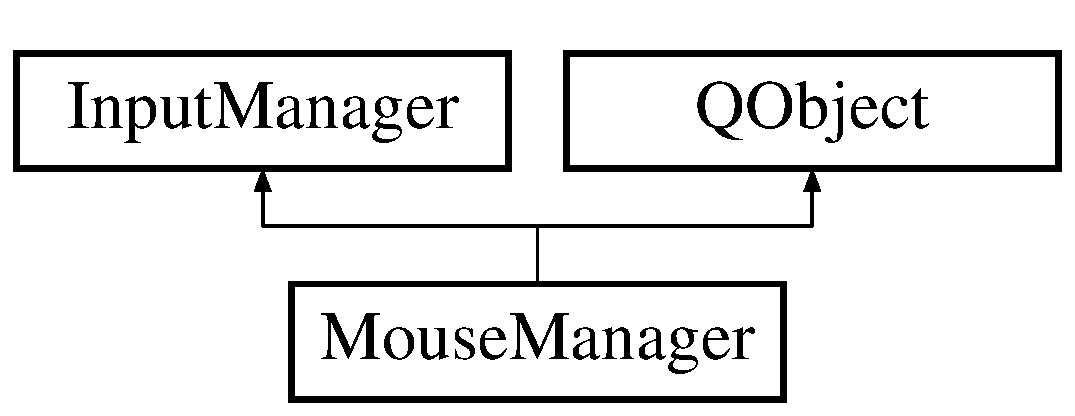
\includegraphics[height=2.000000cm]{class_mouse_manager}
\end{center}
\end{figure}
\subsection*{Public Member Functions}
\begin{DoxyCompactItemize}
\item 
\hyperlink{class_mouse_manager_a6c5c9db90137f189cc49bcabb511fceb}{Mouse\+Manager} ()
\item 
\hyperlink{class_mouse_manager_a88fef729192db0b478421b6d23ac10fe}{$\sim$\+Mouse\+Manager} ()
\item 
bool \hyperlink{class_mouse_manager_a0c06cc77110510a1a36ede06dbc05488}{event\+Filter} (Q\+Object $\ast$, Q\+Event $\ast$event)
\end{DoxyCompactItemize}
\subsection*{Additional Inherited Members}


\subsection{Detailed Description}
Mouse listener class 

\subsection{Constructor \& Destructor Documentation}
\hypertarget{class_mouse_manager_a6c5c9db90137f189cc49bcabb511fceb}{\index{Mouse\+Manager@{Mouse\+Manager}!Mouse\+Manager@{Mouse\+Manager}}
\index{Mouse\+Manager@{Mouse\+Manager}!Mouse\+Manager@{Mouse\+Manager}}
\subsubsection[{Mouse\+Manager}]{\setlength{\rightskip}{0pt plus 5cm}Mouse\+Manager\+::\+Mouse\+Manager (
\begin{DoxyParamCaption}
{}
\end{DoxyParamCaption}
)}}\label{class_mouse_manager_a6c5c9db90137f189cc49bcabb511fceb}
Constructor \hypertarget{class_mouse_manager_a88fef729192db0b478421b6d23ac10fe}{\index{Mouse\+Manager@{Mouse\+Manager}!````~Mouse\+Manager@{$\sim$\+Mouse\+Manager}}
\index{````~Mouse\+Manager@{$\sim$\+Mouse\+Manager}!Mouse\+Manager@{Mouse\+Manager}}
\subsubsection[{$\sim$\+Mouse\+Manager}]{\setlength{\rightskip}{0pt plus 5cm}Mouse\+Manager\+::$\sim$\+Mouse\+Manager (
\begin{DoxyParamCaption}
{}
\end{DoxyParamCaption}
)}}\label{class_mouse_manager_a88fef729192db0b478421b6d23ac10fe}
Destructor 

\subsection{Member Function Documentation}
\hypertarget{class_mouse_manager_a0c06cc77110510a1a36ede06dbc05488}{\index{Mouse\+Manager@{Mouse\+Manager}!event\+Filter@{event\+Filter}}
\index{event\+Filter@{event\+Filter}!Mouse\+Manager@{Mouse\+Manager}}
\subsubsection[{event\+Filter}]{\setlength{\rightskip}{0pt plus 5cm}bool Mouse\+Manager\+::event\+Filter (
\begin{DoxyParamCaption}
\item[{Q\+Object $\ast$}]{, }
\item[{Q\+Event $\ast$}]{event}
\end{DoxyParamCaption}
)}}\label{class_mouse_manager_a0c06cc77110510a1a36ede06dbc05488}
Called when an event occurs on the simon ui 

The documentation for this class was generated from the following files\+:\begin{DoxyCompactItemize}
\item 
Interface\+Managers/mousemanager.\+h\item 
Interface\+Managers/mousemanager.\+cpp\end{DoxyCompactItemize}

\hypertarget{class_pass_dialog}{\section{Pass\+Dialog Class Reference}
\label{class_pass_dialog}\index{Pass\+Dialog@{Pass\+Dialog}}
}


{\ttfamily \#include $<$passdialog.\+h$>$}

Inheritance diagram for Pass\+Dialog\+:\begin{figure}[H]
\begin{center}
\leavevmode
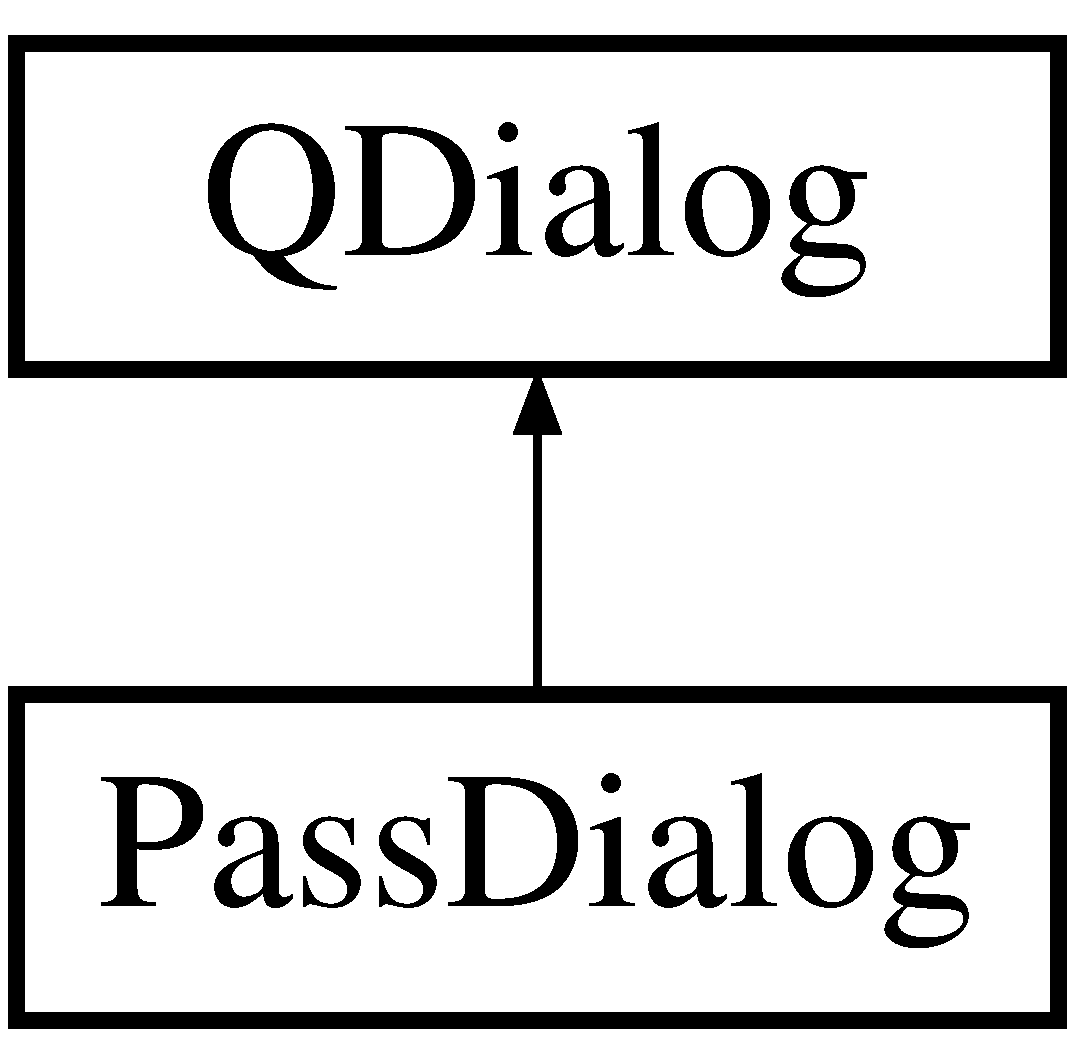
\includegraphics[height=2.000000cm]{class_pass_dialog}
\end{center}
\end{figure}
\subsection*{Public Member Functions}
\begin{DoxyCompactItemize}
\item 
\hyperlink{class_pass_dialog_a2ba0457b15a0ca80f5bb39945890b970}{Pass\+Dialog} (Q\+Widget $\ast$parent=0)
\item 
\hyperlink{class_pass_dialog_ac277cb5dfd04a02e7748a18ae795391f}{$\sim$\+Pass\+Dialog} ()
\item 
void \hyperlink{class_pass_dialog_a85ef04b8b6e869bcf548138b48965b2d}{set\+Title} (Q\+String title)
\item 
void \hyperlink{class_pass_dialog_a9637b02f31c2b9b955a2f274f115f30b}{set\+Subtitle} (Q\+String subtitle)
\end{DoxyCompactItemize}
\subsection*{Protected Member Functions}
\begin{DoxyCompactItemize}
\item 
void \hyperlink{class_pass_dialog_aa1c0796d9caef2bc58365d1304361d89}{close\+Event} (Q\+Close\+Event $\ast$event)
\end{DoxyCompactItemize}


\subsection{Detailed Description}
A dialog box for entering a password 

\subsection{Constructor \& Destructor Documentation}
\hypertarget{class_pass_dialog_a2ba0457b15a0ca80f5bb39945890b970}{\index{Pass\+Dialog@{Pass\+Dialog}!Pass\+Dialog@{Pass\+Dialog}}
\index{Pass\+Dialog@{Pass\+Dialog}!Pass\+Dialog@{Pass\+Dialog}}
\subsubsection[{Pass\+Dialog}]{\setlength{\rightskip}{0pt plus 5cm}Pass\+Dialog\+::\+Pass\+Dialog (
\begin{DoxyParamCaption}
\item[{Q\+Widget $\ast$}]{parent = {\ttfamily 0}}
\end{DoxyParamCaption}
)\hspace{0.3cm}{\ttfamily [explicit]}}}\label{class_pass_dialog_a2ba0457b15a0ca80f5bb39945890b970}
Constructor \hypertarget{class_pass_dialog_ac277cb5dfd04a02e7748a18ae795391f}{\index{Pass\+Dialog@{Pass\+Dialog}!````~Pass\+Dialog@{$\sim$\+Pass\+Dialog}}
\index{````~Pass\+Dialog@{$\sim$\+Pass\+Dialog}!Pass\+Dialog@{Pass\+Dialog}}
\subsubsection[{$\sim$\+Pass\+Dialog}]{\setlength{\rightskip}{0pt plus 5cm}Pass\+Dialog\+::$\sim$\+Pass\+Dialog (
\begin{DoxyParamCaption}
{}
\end{DoxyParamCaption}
)}}\label{class_pass_dialog_ac277cb5dfd04a02e7748a18ae795391f}
Destructor 

\subsection{Member Function Documentation}
\hypertarget{class_pass_dialog_aa1c0796d9caef2bc58365d1304361d89}{\index{Pass\+Dialog@{Pass\+Dialog}!close\+Event@{close\+Event}}
\index{close\+Event@{close\+Event}!Pass\+Dialog@{Pass\+Dialog}}
\subsubsection[{close\+Event}]{\setlength{\rightskip}{0pt plus 5cm}void Pass\+Dialog\+::close\+Event (
\begin{DoxyParamCaption}
\item[{Q\+Close\+Event $\ast$}]{event}
\end{DoxyParamCaption}
)\hspace{0.3cm}{\ttfamily [protected]}}}\label{class_pass_dialog_aa1c0796d9caef2bc58365d1304361d89}
Called when close button is pressed \hypertarget{class_pass_dialog_a9637b02f31c2b9b955a2f274f115f30b}{\index{Pass\+Dialog@{Pass\+Dialog}!set\+Subtitle@{set\+Subtitle}}
\index{set\+Subtitle@{set\+Subtitle}!Pass\+Dialog@{Pass\+Dialog}}
\subsubsection[{set\+Subtitle}]{\setlength{\rightskip}{0pt plus 5cm}void Pass\+Dialog\+::set\+Subtitle (
\begin{DoxyParamCaption}
\item[{Q\+String}]{subtitle}
\end{DoxyParamCaption}
)}}\label{class_pass_dialog_a9637b02f31c2b9b955a2f274f115f30b}
Set dialog subtitle \hypertarget{class_pass_dialog_a85ef04b8b6e869bcf548138b48965b2d}{\index{Pass\+Dialog@{Pass\+Dialog}!set\+Title@{set\+Title}}
\index{set\+Title@{set\+Title}!Pass\+Dialog@{Pass\+Dialog}}
\subsubsection[{set\+Title}]{\setlength{\rightskip}{0pt plus 5cm}void Pass\+Dialog\+::set\+Title (
\begin{DoxyParamCaption}
\item[{Q\+String}]{title}
\end{DoxyParamCaption}
)}}\label{class_pass_dialog_a85ef04b8b6e869bcf548138b48965b2d}
Set dialog title 

The documentation for this class was generated from the following files\+:\begin{DoxyCompactItemize}
\item 
U\+I/passdialog.\+h\item 
U\+I/passdialog.\+cpp\end{DoxyCompactItemize}

\hypertarget{class_leap_1_1_pointable}{\section{Leap\+:\+:Pointable Class Reference}
\label{class_leap_1_1_pointable}\index{Leap\+::\+Pointable@{Leap\+::\+Pointable}}
}


{\ttfamily \#include $<$Leap.\+h$>$}

Inheritance diagram for Leap\+:\+:Pointable\+:\begin{figure}[H]
\begin{center}
\leavevmode
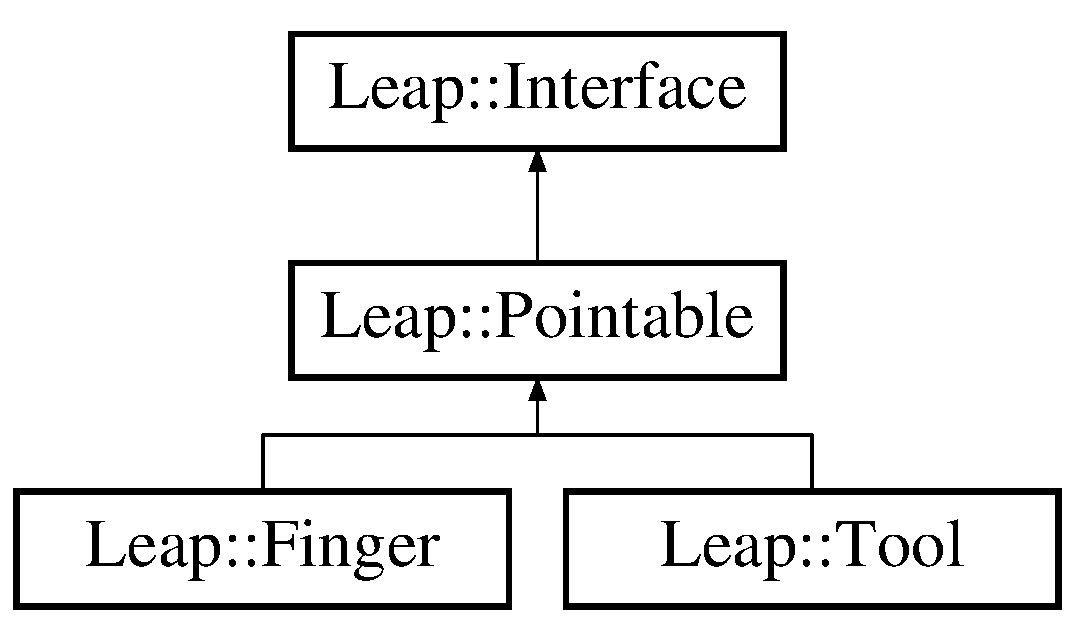
\includegraphics[height=3.000000cm]{class_leap_1_1_pointable}
\end{center}
\end{figure}
\subsection*{Public Types}
\begin{DoxyCompactItemize}
\item 
enum \hyperlink{class_leap_1_1_pointable_ad6e50b9878b8c1fdf899b5e09721deef}{Zone} \{ \hyperlink{class_leap_1_1_pointable_ad6e50b9878b8c1fdf899b5e09721deefa4c1e87f878b5a0a3d1ac4903f92e29fe}{Z\+O\+N\+E\+\_\+\+N\+O\+N\+E} = 0, 
\hyperlink{class_leap_1_1_pointable_ad6e50b9878b8c1fdf899b5e09721deefad8f42b8833b8233e2b196863b5937f3c}{Z\+O\+N\+E\+\_\+\+H\+O\+V\+E\+R\+I\+N\+G} = 1, 
\hyperlink{class_leap_1_1_pointable_ad6e50b9878b8c1fdf899b5e09721deefa9ccf7859ad8c4f411779d04fbdb23e23}{Z\+O\+N\+E\+\_\+\+T\+O\+U\+C\+H\+I\+N\+G} = 2
 \}
\end{DoxyCompactItemize}
\subsection*{Public Member Functions}
\begin{DoxyCompactItemize}
\item 
\hypertarget{class_leap_1_1_pointable_a508745ae2e3402b4f754028197575457}{{\bfseries Pointable} (Pointable\+Implementation $\ast$)}\label{class_leap_1_1_pointable_a508745ae2e3402b4f754028197575457}

\item 
\hypertarget{class_leap_1_1_pointable_a20653c8953646cef96d78684f7e2c349}{{\bfseries Pointable} (Finger\+Implementation $\ast$)}\label{class_leap_1_1_pointable_a20653c8953646cef96d78684f7e2c349}

\item 
\hypertarget{class_leap_1_1_pointable_afa744fc2a9d312958a06d0d0a93f6799}{{\bfseries Pointable} (Tool\+Implementation $\ast$)}\label{class_leap_1_1_pointable_afa744fc2a9d312958a06d0d0a93f6799}

\item 
L\+E\+A\+P\+\_\+\+E\+X\+P\+O\+R\+T \hyperlink{class_leap_1_1_pointable_a5b42d880b673daa25c938d9fcf8d93eb}{Pointable} ()
\item 
L\+E\+A\+P\+\_\+\+E\+X\+P\+O\+R\+T int32\+\_\+t \hyperlink{class_leap_1_1_pointable_ae9f83eb705c71bb7b424f886942b542b}{id} () const 
\item 
L\+E\+A\+P\+\_\+\+E\+X\+P\+O\+R\+T \hyperlink{class_leap_1_1_frame}{Frame} \hyperlink{class_leap_1_1_pointable_ad9e1c4df8ce62d591ca52e432cf4848f}{frame} () const 
\item 
L\+E\+A\+P\+\_\+\+E\+X\+P\+O\+R\+T \hyperlink{class_leap_1_1_hand}{Hand} \hyperlink{class_leap_1_1_pointable_a7858c2e5b5bf614ba3991e5237feed9a}{hand} () const 
\item 
L\+E\+A\+P\+\_\+\+E\+X\+P\+O\+R\+T \hyperlink{struct_leap_1_1_vector}{Vector} \hyperlink{class_leap_1_1_pointable_aaa7d42165f9511f18a20d3b7441a7eb5}{tip\+Position} () const 
\item 
L\+E\+A\+P\+\_\+\+E\+X\+P\+O\+R\+T \hyperlink{struct_leap_1_1_vector}{Vector} \hyperlink{class_leap_1_1_pointable_abf52ec088026b9d1a7f46ff445c130e3}{tip\+Velocity} () const 
\item 
L\+E\+A\+P\+\_\+\+E\+X\+P\+O\+R\+T \hyperlink{struct_leap_1_1_vector}{Vector} \hyperlink{class_leap_1_1_pointable_adf395a6689ebf00a17dd6d33a4aeaccd}{direction} () const 
\item 
L\+E\+A\+P\+\_\+\+E\+X\+P\+O\+R\+T float \hyperlink{class_leap_1_1_pointable_a1287f947168fcd1856098f7628509602}{width} () const 
\item 
L\+E\+A\+P\+\_\+\+E\+X\+P\+O\+R\+T float \hyperlink{class_leap_1_1_pointable_ab28e9e4be4d507b6093b6aa015cac816}{length} () const 
\item 
L\+E\+A\+P\+\_\+\+E\+X\+P\+O\+R\+T bool \hyperlink{class_leap_1_1_pointable_acb22151412f46b6be8b773986452eba8}{is\+Finger} () const 
\item 
L\+E\+A\+P\+\_\+\+E\+X\+P\+O\+R\+T bool \hyperlink{class_leap_1_1_pointable_ac10f09626b790dd5867411748242c437}{is\+Tool} () const 
\item 
L\+E\+A\+P\+\_\+\+E\+X\+P\+O\+R\+T bool \hyperlink{class_leap_1_1_pointable_a124f21a619df4fb338d1ce8a7a6d3341}{is\+Valid} () const 
\item 
L\+E\+A\+P\+\_\+\+E\+X\+P\+O\+R\+T \hyperlink{class_leap_1_1_pointable_ad6e50b9878b8c1fdf899b5e09721deef}{Zone} \hyperlink{class_leap_1_1_pointable_a6cc17d698df38fe84bbf507a8def65ac}{touch\+Zone} () const 
\item 
L\+E\+A\+P\+\_\+\+E\+X\+P\+O\+R\+T float \hyperlink{class_leap_1_1_pointable_a20ea59c9efc41133255301a898d48592}{touch\+Distance} () const 
\item 
L\+E\+A\+P\+\_\+\+E\+X\+P\+O\+R\+T \hyperlink{struct_leap_1_1_vector}{Vector} \hyperlink{class_leap_1_1_pointable_ae80139b0c44868f570bdcb6f2f7417ec}{stabilized\+Tip\+Position} () const 
\item 
L\+E\+A\+P\+\_\+\+E\+X\+P\+O\+R\+T float \hyperlink{class_leap_1_1_pointable_a7fbc47bef4194a619ca0a0d2756ed48b}{time\+Visible} () const 
\item 
L\+E\+A\+P\+\_\+\+E\+X\+P\+O\+R\+T bool \hyperlink{class_leap_1_1_pointable_a1b5dd8315f944e3dd2d7f7247c28781f}{operator==} (const \hyperlink{class_leap_1_1_pointable}{Pointable} \&) const 
\item 
L\+E\+A\+P\+\_\+\+E\+X\+P\+O\+R\+T bool \hyperlink{class_leap_1_1_pointable_af6f3872bfd84553e9ca53c49457f8c1f}{operator!=} (const \hyperlink{class_leap_1_1_pointable}{Pointable} \&) const 
\item 
L\+E\+A\+P\+\_\+\+E\+X\+P\+O\+R\+T std\+::string \hyperlink{class_leap_1_1_pointable_ab40247dc558a04b53110da3c45059371}{to\+String} () const 
\end{DoxyCompactItemize}
\subsection*{Static Public Member Functions}
\begin{DoxyCompactItemize}
\item 
static L\+E\+A\+P\+\_\+\+E\+X\+P\+O\+R\+T const \\*
\hyperlink{class_leap_1_1_pointable}{Pointable} \& \hyperlink{class_leap_1_1_pointable_a2d66e938c10bf54778fdfe5abf7dd77d}{invalid} ()
\end{DoxyCompactItemize}
\subsection*{Friends}
\begin{DoxyCompactItemize}
\item 
L\+E\+A\+P\+\_\+\+E\+X\+P\+O\+R\+T friend std\+::ostream \& \hyperlink{class_leap_1_1_pointable_a3e0fe2f963f09cfaf2d4dc9b93c85b4d}{operator$<$$<$} (std\+::ostream \&, const \hyperlink{class_leap_1_1_pointable}{Pointable} \&)
\end{DoxyCompactItemize}
\subsection*{Additional Inherited Members}


\subsection{Detailed Description}
The \hyperlink{class_leap_1_1_pointable}{Pointable} class reports the physical characteristics of a detected finger or tool.

Both fingers and tools are classified as \hyperlink{class_leap_1_1_pointable}{Pointable} objects. Use the \hyperlink{class_leap_1_1_pointable_acb22151412f46b6be8b773986452eba8}{Pointable\+::is\+Finger()} function to determine whether a \hyperlink{class_leap_1_1_pointable}{Pointable} object represents a finger. Use the \hyperlink{class_leap_1_1_pointable_ac10f09626b790dd5867411748242c437}{Pointable\+::is\+Tool()} function to determine whether a \hyperlink{class_leap_1_1_pointable}{Pointable} object represents a tool. The Leap Motion software classifies a detected entity as a tool when it is thinner, straighter, and longer than a typical finger.

To provide touch emulation, the Leap Motion software associates a floating touch plane that adapts to the user's finger movement and hand posture. The Leap Motion interprets purposeful movements toward this plane as potential touch points. The \hyperlink{class_leap_1_1_pointable}{Pointable} class reports touch state with the touch\+Zone and touch\+Distance values.

Note that \hyperlink{class_leap_1_1_pointable}{Pointable} objects can be invalid, which means that they do not contain valid tracking data and do not correspond to a physical entity. Invalid \hyperlink{class_leap_1_1_pointable}{Pointable} objects can be the result of asking for a \hyperlink{class_leap_1_1_pointable}{Pointable} object using an I\+D from an earlier frame when no \hyperlink{class_leap_1_1_pointable}{Pointable} objects with that I\+D exist in the current frame. A \hyperlink{class_leap_1_1_pointable}{Pointable} object created from the \hyperlink{class_leap_1_1_pointable}{Pointable} constructor is also invalid. Test for validity with the \hyperlink{class_leap_1_1_pointable_a124f21a619df4fb338d1ce8a7a6d3341}{Pointable\+::is\+Valid()} function.

\begin{DoxySince}{Since}
1.\+0 
\end{DoxySince}


\subsection{Member Enumeration Documentation}
\hypertarget{class_leap_1_1_pointable_ad6e50b9878b8c1fdf899b5e09721deef}{\index{Leap\+::\+Pointable@{Leap\+::\+Pointable}!Zone@{Zone}}
\index{Zone@{Zone}!Leap\+::\+Pointable@{Leap\+::\+Pointable}}
\subsubsection[{Zone}]{\setlength{\rightskip}{0pt plus 5cm}enum {\bf Leap\+::\+Pointable\+::\+Zone}}}\label{class_leap_1_1_pointable_ad6e50b9878b8c1fdf899b5e09721deef}
Defines the values for reporting the state of a \hyperlink{class_leap_1_1_pointable}{Pointable} object in relation to an adaptive touch plane. \begin{DoxySince}{Since}
1.\+0 
\end{DoxySince}
\begin{Desc}
\item[Enumerator]\par
\begin{description}
\index{Z\+O\+N\+E\+\_\+\+N\+O\+N\+E@{Z\+O\+N\+E\+\_\+\+N\+O\+N\+E}!Leap\+::\+Pointable@{Leap\+::\+Pointable}}\index{Leap\+::\+Pointable@{Leap\+::\+Pointable}!Z\+O\+N\+E\+\_\+\+N\+O\+N\+E@{Z\+O\+N\+E\+\_\+\+N\+O\+N\+E}}\item[{\em 
\hypertarget{class_leap_1_1_pointable_ad6e50b9878b8c1fdf899b5e09721deefa4c1e87f878b5a0a3d1ac4903f92e29fe}{Z\+O\+N\+E\+\_\+\+N\+O\+N\+E}\label{class_leap_1_1_pointable_ad6e50b9878b8c1fdf899b5e09721deefa4c1e87f878b5a0a3d1ac4903f92e29fe}
}]The \hyperlink{class_leap_1_1_pointable}{Pointable} object is too far from the plane to be considered hovering or touching. \begin{DoxySince}{Since}
1.\+0 
\end{DoxySince}
\index{Z\+O\+N\+E\+\_\+\+H\+O\+V\+E\+R\+I\+N\+G@{Z\+O\+N\+E\+\_\+\+H\+O\+V\+E\+R\+I\+N\+G}!Leap\+::\+Pointable@{Leap\+::\+Pointable}}\index{Leap\+::\+Pointable@{Leap\+::\+Pointable}!Z\+O\+N\+E\+\_\+\+H\+O\+V\+E\+R\+I\+N\+G@{Z\+O\+N\+E\+\_\+\+H\+O\+V\+E\+R\+I\+N\+G}}\item[{\em 
\hypertarget{class_leap_1_1_pointable_ad6e50b9878b8c1fdf899b5e09721deefad8f42b8833b8233e2b196863b5937f3c}{Z\+O\+N\+E\+\_\+\+H\+O\+V\+E\+R\+I\+N\+G}\label{class_leap_1_1_pointable_ad6e50b9878b8c1fdf899b5e09721deefad8f42b8833b8233e2b196863b5937f3c}
}]The \hyperlink{class_leap_1_1_pointable}{Pointable} object is close to, but not touching the plane. \begin{DoxySince}{Since}
1.\+0 
\end{DoxySince}
\index{Z\+O\+N\+E\+\_\+\+T\+O\+U\+C\+H\+I\+N\+G@{Z\+O\+N\+E\+\_\+\+T\+O\+U\+C\+H\+I\+N\+G}!Leap\+::\+Pointable@{Leap\+::\+Pointable}}\index{Leap\+::\+Pointable@{Leap\+::\+Pointable}!Z\+O\+N\+E\+\_\+\+T\+O\+U\+C\+H\+I\+N\+G@{Z\+O\+N\+E\+\_\+\+T\+O\+U\+C\+H\+I\+N\+G}}\item[{\em 
\hypertarget{class_leap_1_1_pointable_ad6e50b9878b8c1fdf899b5e09721deefa9ccf7859ad8c4f411779d04fbdb23e23}{Z\+O\+N\+E\+\_\+\+T\+O\+U\+C\+H\+I\+N\+G}\label{class_leap_1_1_pointable_ad6e50b9878b8c1fdf899b5e09721deefa9ccf7859ad8c4f411779d04fbdb23e23}
}]The \hyperlink{class_leap_1_1_pointable}{Pointable} has penetrated the plane. \begin{DoxySince}{Since}
1.\+0 
\end{DoxySince}
\end{description}
\end{Desc}


\subsection{Constructor \& Destructor Documentation}
\hypertarget{class_leap_1_1_pointable_a5b42d880b673daa25c938d9fcf8d93eb}{\index{Leap\+::\+Pointable@{Leap\+::\+Pointable}!Pointable@{Pointable}}
\index{Pointable@{Pointable}!Leap\+::\+Pointable@{Leap\+::\+Pointable}}
\subsubsection[{Pointable}]{\setlength{\rightskip}{0pt plus 5cm}L\+E\+A\+P\+\_\+\+E\+X\+P\+O\+R\+T Leap\+::\+Pointable\+::\+Pointable (
\begin{DoxyParamCaption}
{}
\end{DoxyParamCaption}
)}}\label{class_leap_1_1_pointable_a5b42d880b673daa25c938d9fcf8d93eb}
Constructs a \hyperlink{class_leap_1_1_pointable}{Pointable} object.

An uninitialized pointable is considered invalid. Get valid \hyperlink{class_leap_1_1_pointable}{Pointable} objects from a \hyperlink{class_leap_1_1_frame}{Frame} or a \hyperlink{class_leap_1_1_hand}{Hand} object. \begin{DoxySince}{Since}
1.\+0 
\end{DoxySince}


\subsection{Member Function Documentation}
\hypertarget{class_leap_1_1_pointable_adf395a6689ebf00a17dd6d33a4aeaccd}{\index{Leap\+::\+Pointable@{Leap\+::\+Pointable}!direction@{direction}}
\index{direction@{direction}!Leap\+::\+Pointable@{Leap\+::\+Pointable}}
\subsubsection[{direction}]{\setlength{\rightskip}{0pt plus 5cm}L\+E\+A\+P\+\_\+\+E\+X\+P\+O\+R\+T {\bf Vector} Leap\+::\+Pointable\+::direction (
\begin{DoxyParamCaption}
{}
\end{DoxyParamCaption}
) const}}\label{class_leap_1_1_pointable_adf395a6689ebf00a17dd6d33a4aeaccd}
The direction in which this finger or tool is pointing.

The direction is expressed as a unit vector pointing in the same direction as the tip.



\begin{DoxyReturn}{Returns}
The \hyperlink{struct_leap_1_1_vector}{Vector} pointing in the same direction as the tip of this \hyperlink{class_leap_1_1_pointable}{Pointable} object. 
\end{DoxyReturn}
\begin{DoxySince}{Since}
1.\+0 
\end{DoxySince}
\hypertarget{class_leap_1_1_pointable_ad9e1c4df8ce62d591ca52e432cf4848f}{\index{Leap\+::\+Pointable@{Leap\+::\+Pointable}!frame@{frame}}
\index{frame@{frame}!Leap\+::\+Pointable@{Leap\+::\+Pointable}}
\subsubsection[{frame}]{\setlength{\rightskip}{0pt plus 5cm}L\+E\+A\+P\+\_\+\+E\+X\+P\+O\+R\+T {\bf Frame} Leap\+::\+Pointable\+::frame (
\begin{DoxyParamCaption}
{}
\end{DoxyParamCaption}
) const}}\label{class_leap_1_1_pointable_ad9e1c4df8ce62d591ca52e432cf4848f}
The \hyperlink{class_leap_1_1_frame}{Frame} associated with this \hyperlink{class_leap_1_1_pointable}{Pointable} object.

\begin{DoxyReturn}{Returns}
The associated \hyperlink{class_leap_1_1_frame}{Frame} object, if available; otherwise, an invalid \hyperlink{class_leap_1_1_frame}{Frame} object is returned. 
\end{DoxyReturn}
\begin{DoxySince}{Since}
1.\+0 
\end{DoxySince}
\hypertarget{class_leap_1_1_pointable_a7858c2e5b5bf614ba3991e5237feed9a}{\index{Leap\+::\+Pointable@{Leap\+::\+Pointable}!hand@{hand}}
\index{hand@{hand}!Leap\+::\+Pointable@{Leap\+::\+Pointable}}
\subsubsection[{hand}]{\setlength{\rightskip}{0pt plus 5cm}L\+E\+A\+P\+\_\+\+E\+X\+P\+O\+R\+T {\bf Hand} Leap\+::\+Pointable\+::hand (
\begin{DoxyParamCaption}
{}
\end{DoxyParamCaption}
) const}}\label{class_leap_1_1_pointable_a7858c2e5b5bf614ba3991e5237feed9a}
The \hyperlink{class_leap_1_1_hand}{Hand} associated with this finger or tool.

\begin{DoxyReturn}{Returns}
The associated \hyperlink{class_leap_1_1_hand}{Hand} object, if available; otherwise, an invalid \hyperlink{class_leap_1_1_hand}{Hand} object is returned. 
\end{DoxyReturn}
\begin{DoxySince}{Since}
1.\+0 
\end{DoxySince}
\hypertarget{class_leap_1_1_pointable_ae9f83eb705c71bb7b424f886942b542b}{\index{Leap\+::\+Pointable@{Leap\+::\+Pointable}!id@{id}}
\index{id@{id}!Leap\+::\+Pointable@{Leap\+::\+Pointable}}
\subsubsection[{id}]{\setlength{\rightskip}{0pt plus 5cm}L\+E\+A\+P\+\_\+\+E\+X\+P\+O\+R\+T int32\+\_\+t Leap\+::\+Pointable\+::id (
\begin{DoxyParamCaption}
{}
\end{DoxyParamCaption}
) const}}\label{class_leap_1_1_pointable_ae9f83eb705c71bb7b424f886942b542b}
A unique I\+D assigned to this \hyperlink{class_leap_1_1_pointable}{Pointable} object, whose value remains the same across consecutive frames while the tracked finger or tool remains visible. If tracking is lost (for example, when a finger is occluded by another finger or when it is withdrawn from the Leap Motion \hyperlink{class_leap_1_1_controller}{Controller} field of view), the Leap Motion software may assign a new I\+D when it detects the entity in a future frame.

Use the I\+D value with the \hyperlink{class_leap_1_1_frame_a965d1e23e9ad84420359711768ff1fab}{Frame\+::pointable()} function to find this \hyperlink{class_leap_1_1_pointable}{Pointable} object in future frames.

I\+Ds should be from 1 to 100 (inclusive). If more than 100 objects are tracked an I\+Ds of -\/1 will be used until an I\+D in the defined range is available.

\begin{DoxyReturn}{Returns}
The I\+D assigned to this \hyperlink{class_leap_1_1_pointable}{Pointable} object. 
\end{DoxyReturn}
\begin{DoxySince}{Since}
1.\+0 
\end{DoxySince}
\hypertarget{class_leap_1_1_pointable_a2d66e938c10bf54778fdfe5abf7dd77d}{\index{Leap\+::\+Pointable@{Leap\+::\+Pointable}!invalid@{invalid}}
\index{invalid@{invalid}!Leap\+::\+Pointable@{Leap\+::\+Pointable}}
\subsubsection[{invalid}]{\setlength{\rightskip}{0pt plus 5cm}static L\+E\+A\+P\+\_\+\+E\+X\+P\+O\+R\+T const {\bf Pointable}\& Leap\+::\+Pointable\+::invalid (
\begin{DoxyParamCaption}
{}
\end{DoxyParamCaption}
)\hspace{0.3cm}{\ttfamily [static]}}}\label{class_leap_1_1_pointable_a2d66e938c10bf54778fdfe5abf7dd77d}
Returns an invalid \hyperlink{class_leap_1_1_pointable}{Pointable} object.

You can use the instance returned by this function in comparisons testing whether a given \hyperlink{class_leap_1_1_pointable}{Pointable} instance is valid or invalid. (You can also use the \hyperlink{class_leap_1_1_pointable_a124f21a619df4fb338d1ce8a7a6d3341}{Pointable\+::is\+Valid()} function.)

\begin{DoxyReturn}{Returns}
The invalid \hyperlink{class_leap_1_1_pointable}{Pointable} instance. 
\end{DoxyReturn}
\begin{DoxySince}{Since}
1.\+0 
\end{DoxySince}
\hypertarget{class_leap_1_1_pointable_acb22151412f46b6be8b773986452eba8}{\index{Leap\+::\+Pointable@{Leap\+::\+Pointable}!is\+Finger@{is\+Finger}}
\index{is\+Finger@{is\+Finger}!Leap\+::\+Pointable@{Leap\+::\+Pointable}}
\subsubsection[{is\+Finger}]{\setlength{\rightskip}{0pt plus 5cm}L\+E\+A\+P\+\_\+\+E\+X\+P\+O\+R\+T bool Leap\+::\+Pointable\+::is\+Finger (
\begin{DoxyParamCaption}
{}
\end{DoxyParamCaption}
) const}}\label{class_leap_1_1_pointable_acb22151412f46b6be8b773986452eba8}
Whether or not the \hyperlink{class_leap_1_1_pointable}{Pointable} is believed to be a finger. Fingers are generally shorter, thicker, and less straight than tools.

\begin{DoxyReturn}{Returns}
True, if this \hyperlink{class_leap_1_1_pointable}{Pointable} is classified as a finger. 
\end{DoxyReturn}
\begin{DoxySince}{Since}
1.\+0 
\end{DoxySince}
\hypertarget{class_leap_1_1_pointable_ac10f09626b790dd5867411748242c437}{\index{Leap\+::\+Pointable@{Leap\+::\+Pointable}!is\+Tool@{is\+Tool}}
\index{is\+Tool@{is\+Tool}!Leap\+::\+Pointable@{Leap\+::\+Pointable}}
\subsubsection[{is\+Tool}]{\setlength{\rightskip}{0pt plus 5cm}L\+E\+A\+P\+\_\+\+E\+X\+P\+O\+R\+T bool Leap\+::\+Pointable\+::is\+Tool (
\begin{DoxyParamCaption}
{}
\end{DoxyParamCaption}
) const}}\label{class_leap_1_1_pointable_ac10f09626b790dd5867411748242c437}
Whether or not the \hyperlink{class_leap_1_1_pointable}{Pointable} is believed to be a tool. Tools are generally longer, thinner, and straighter than fingers.

\begin{DoxyReturn}{Returns}
True, if this \hyperlink{class_leap_1_1_pointable}{Pointable} is classified as a tool. 
\end{DoxyReturn}
\begin{DoxySince}{Since}
1.\+0 
\end{DoxySince}
\hypertarget{class_leap_1_1_pointable_a124f21a619df4fb338d1ce8a7a6d3341}{\index{Leap\+::\+Pointable@{Leap\+::\+Pointable}!is\+Valid@{is\+Valid}}
\index{is\+Valid@{is\+Valid}!Leap\+::\+Pointable@{Leap\+::\+Pointable}}
\subsubsection[{is\+Valid}]{\setlength{\rightskip}{0pt plus 5cm}L\+E\+A\+P\+\_\+\+E\+X\+P\+O\+R\+T bool Leap\+::\+Pointable\+::is\+Valid (
\begin{DoxyParamCaption}
{}
\end{DoxyParamCaption}
) const}}\label{class_leap_1_1_pointable_a124f21a619df4fb338d1ce8a7a6d3341}
Reports whether this is a valid \hyperlink{class_leap_1_1_pointable}{Pointable} object.

\begin{DoxyReturn}{Returns}
True, if this \hyperlink{class_leap_1_1_pointable}{Pointable} object contains valid tracking data. 
\end{DoxyReturn}
\begin{DoxySince}{Since}
1.\+0 
\end{DoxySince}
\hypertarget{class_leap_1_1_pointable_ab28e9e4be4d507b6093b6aa015cac816}{\index{Leap\+::\+Pointable@{Leap\+::\+Pointable}!length@{length}}
\index{length@{length}!Leap\+::\+Pointable@{Leap\+::\+Pointable}}
\subsubsection[{length}]{\setlength{\rightskip}{0pt plus 5cm}L\+E\+A\+P\+\_\+\+E\+X\+P\+O\+R\+T float Leap\+::\+Pointable\+::length (
\begin{DoxyParamCaption}
{}
\end{DoxyParamCaption}
) const}}\label{class_leap_1_1_pointable_ab28e9e4be4d507b6093b6aa015cac816}
The estimated length of the finger or tool in millimeters.

The reported length is the visible length of the finger or tool from the hand to tip. If the length isn't known, then a value of 0 is returned.

\begin{DoxyReturn}{Returns}
The estimated length of this \hyperlink{class_leap_1_1_pointable}{Pointable} object. 
\end{DoxyReturn}
\begin{DoxySince}{Since}
1.\+0 
\end{DoxySince}
\hypertarget{class_leap_1_1_pointable_af6f3872bfd84553e9ca53c49457f8c1f}{\index{Leap\+::\+Pointable@{Leap\+::\+Pointable}!operator"!=@{operator"!=}}
\index{operator"!=@{operator"!=}!Leap\+::\+Pointable@{Leap\+::\+Pointable}}
\subsubsection[{operator"!=}]{\setlength{\rightskip}{0pt plus 5cm}L\+E\+A\+P\+\_\+\+E\+X\+P\+O\+R\+T bool Leap\+::\+Pointable\+::operator!= (
\begin{DoxyParamCaption}
\item[{const {\bf Pointable} \&}]{}
\end{DoxyParamCaption}
) const}}\label{class_leap_1_1_pointable_af6f3872bfd84553e9ca53c49457f8c1f}
Compare \hyperlink{class_leap_1_1_pointable}{Pointable} object inequality. Two \hyperlink{class_leap_1_1_pointable}{Pointable} objects are equal if and only if both \hyperlink{class_leap_1_1_pointable}{Pointable} objects represent the exact same physical entities in the same frame and both \hyperlink{class_leap_1_1_pointable}{Pointable} objects are valid. \begin{DoxySince}{Since}
1.\+0 
\end{DoxySince}
\hypertarget{class_leap_1_1_pointable_a1b5dd8315f944e3dd2d7f7247c28781f}{\index{Leap\+::\+Pointable@{Leap\+::\+Pointable}!operator==@{operator==}}
\index{operator==@{operator==}!Leap\+::\+Pointable@{Leap\+::\+Pointable}}
\subsubsection[{operator==}]{\setlength{\rightskip}{0pt plus 5cm}L\+E\+A\+P\+\_\+\+E\+X\+P\+O\+R\+T bool Leap\+::\+Pointable\+::operator== (
\begin{DoxyParamCaption}
\item[{const {\bf Pointable} \&}]{}
\end{DoxyParamCaption}
) const}}\label{class_leap_1_1_pointable_a1b5dd8315f944e3dd2d7f7247c28781f}
Compare \hyperlink{class_leap_1_1_pointable}{Pointable} object equality. Two \hyperlink{class_leap_1_1_pointable}{Pointable} objects are equal if and only if both \hyperlink{class_leap_1_1_pointable}{Pointable} objects represent the exact same physical entities in the same frame and both \hyperlink{class_leap_1_1_pointable}{Pointable} objects are valid. \begin{DoxySince}{Since}
1.\+0 
\end{DoxySince}
\hypertarget{class_leap_1_1_pointable_ae80139b0c44868f570bdcb6f2f7417ec}{\index{Leap\+::\+Pointable@{Leap\+::\+Pointable}!stabilized\+Tip\+Position@{stabilized\+Tip\+Position}}
\index{stabilized\+Tip\+Position@{stabilized\+Tip\+Position}!Leap\+::\+Pointable@{Leap\+::\+Pointable}}
\subsubsection[{stabilized\+Tip\+Position}]{\setlength{\rightskip}{0pt plus 5cm}L\+E\+A\+P\+\_\+\+E\+X\+P\+O\+R\+T {\bf Vector} Leap\+::\+Pointable\+::stabilized\+Tip\+Position (
\begin{DoxyParamCaption}
{}
\end{DoxyParamCaption}
) const}}\label{class_leap_1_1_pointable_ae80139b0c44868f570bdcb6f2f7417ec}
The stabilized tip position of this \hyperlink{class_leap_1_1_pointable}{Pointable}.

Smoothing and stabilization is performed in order to make this value more suitable for interaction with 2\+D content. The stabilized position lags behind the tip position by a variable amount, depending primarily on the speed of movement.

\begin{DoxyReturn}{Returns}
A modified tip position of this \hyperlink{class_leap_1_1_pointable}{Pointable} object with some additional smoothing and stabilization applied. 
\end{DoxyReturn}
\begin{DoxySince}{Since}
1.\+0 
\end{DoxySince}
\hypertarget{class_leap_1_1_pointable_a7fbc47bef4194a619ca0a0d2756ed48b}{\index{Leap\+::\+Pointable@{Leap\+::\+Pointable}!time\+Visible@{time\+Visible}}
\index{time\+Visible@{time\+Visible}!Leap\+::\+Pointable@{Leap\+::\+Pointable}}
\subsubsection[{time\+Visible}]{\setlength{\rightskip}{0pt plus 5cm}L\+E\+A\+P\+\_\+\+E\+X\+P\+O\+R\+T float Leap\+::\+Pointable\+::time\+Visible (
\begin{DoxyParamCaption}
{}
\end{DoxyParamCaption}
) const}}\label{class_leap_1_1_pointable_a7fbc47bef4194a619ca0a0d2756ed48b}
The duration of time this \hyperlink{class_leap_1_1_pointable}{Pointable} has been visible to the Leap Motion \hyperlink{class_leap_1_1_controller}{Controller}.

\begin{DoxyReturn}{Returns}
The duration (in seconds) that this \hyperlink{class_leap_1_1_pointable}{Pointable} has been tracked. 
\end{DoxyReturn}
\begin{DoxySince}{Since}
1.\+0 
\end{DoxySince}
\hypertarget{class_leap_1_1_pointable_aaa7d42165f9511f18a20d3b7441a7eb5}{\index{Leap\+::\+Pointable@{Leap\+::\+Pointable}!tip\+Position@{tip\+Position}}
\index{tip\+Position@{tip\+Position}!Leap\+::\+Pointable@{Leap\+::\+Pointable}}
\subsubsection[{tip\+Position}]{\setlength{\rightskip}{0pt plus 5cm}L\+E\+A\+P\+\_\+\+E\+X\+P\+O\+R\+T {\bf Vector} Leap\+::\+Pointable\+::tip\+Position (
\begin{DoxyParamCaption}
{}
\end{DoxyParamCaption}
) const}}\label{class_leap_1_1_pointable_aaa7d42165f9511f18a20d3b7441a7eb5}
The tip position in millimeters from the Leap Motion origin.

\begin{DoxyReturn}{Returns}
The \hyperlink{struct_leap_1_1_vector}{Vector} containing the coordinates of the tip position. 
\end{DoxyReturn}
\begin{DoxySince}{Since}
1.\+0 
\end{DoxySince}
\hypertarget{class_leap_1_1_pointable_abf52ec088026b9d1a7f46ff445c130e3}{\index{Leap\+::\+Pointable@{Leap\+::\+Pointable}!tip\+Velocity@{tip\+Velocity}}
\index{tip\+Velocity@{tip\+Velocity}!Leap\+::\+Pointable@{Leap\+::\+Pointable}}
\subsubsection[{tip\+Velocity}]{\setlength{\rightskip}{0pt plus 5cm}L\+E\+A\+P\+\_\+\+E\+X\+P\+O\+R\+T {\bf Vector} Leap\+::\+Pointable\+::tip\+Velocity (
\begin{DoxyParamCaption}
{}
\end{DoxyParamCaption}
) const}}\label{class_leap_1_1_pointable_abf52ec088026b9d1a7f46ff445c130e3}
The rate of change of the tip position in millimeters/second.

\begin{DoxyReturn}{Returns}
The \hyperlink{struct_leap_1_1_vector}{Vector} containing the coordinates of the tip velocity. 
\end{DoxyReturn}
\begin{DoxySince}{Since}
1.\+0 
\end{DoxySince}
\hypertarget{class_leap_1_1_pointable_ab40247dc558a04b53110da3c45059371}{\index{Leap\+::\+Pointable@{Leap\+::\+Pointable}!to\+String@{to\+String}}
\index{to\+String@{to\+String}!Leap\+::\+Pointable@{Leap\+::\+Pointable}}
\subsubsection[{to\+String}]{\setlength{\rightskip}{0pt plus 5cm}L\+E\+A\+P\+\_\+\+E\+X\+P\+O\+R\+T std\+::string Leap\+::\+Pointable\+::to\+String (
\begin{DoxyParamCaption}
{}
\end{DoxyParamCaption}
) const}}\label{class_leap_1_1_pointable_ab40247dc558a04b53110da3c45059371}
A string containing a brief, human readable description of the \hyperlink{class_leap_1_1_pointable}{Pointable} object.

\begin{DoxyReturn}{Returns}
A description of the \hyperlink{class_leap_1_1_pointable}{Pointable} object as a string. 
\end{DoxyReturn}
\begin{DoxySince}{Since}
1.\+0 
\end{DoxySince}
\hypertarget{class_leap_1_1_pointable_a20ea59c9efc41133255301a898d48592}{\index{Leap\+::\+Pointable@{Leap\+::\+Pointable}!touch\+Distance@{touch\+Distance}}
\index{touch\+Distance@{touch\+Distance}!Leap\+::\+Pointable@{Leap\+::\+Pointable}}
\subsubsection[{touch\+Distance}]{\setlength{\rightskip}{0pt plus 5cm}L\+E\+A\+P\+\_\+\+E\+X\+P\+O\+R\+T float Leap\+::\+Pointable\+::touch\+Distance (
\begin{DoxyParamCaption}
{}
\end{DoxyParamCaption}
) const}}\label{class_leap_1_1_pointable_a20ea59c9efc41133255301a898d48592}
A value proportional to the distance between this \hyperlink{class_leap_1_1_pointable}{Pointable} object and the adaptive touch plane.



The touch distance is a value in the range \mbox{[}-\/1, 1\mbox{]}. The value 1.\+0 indicates the \hyperlink{class_leap_1_1_pointable}{Pointable} is at the far edge of the hovering zone. The value 0 indicates the \hyperlink{class_leap_1_1_pointable}{Pointable} is just entering the touching zone. A value of -\/1.\+0 indicates the \hyperlink{class_leap_1_1_pointable}{Pointable} is firmly within the touching zone. Values in between are proportional to the distance from the plane. Thus, the touch\+Distance of 0.\+5 indicates that the \hyperlink{class_leap_1_1_pointable}{Pointable} is halfway into the hovering zone.

You can use the touch\+Distance value to modulate visual feedback given to the user as their fingers close in on a touch target, such as a button.

\begin{DoxyReturn}{Returns}
The normalized touch distance of this \hyperlink{class_leap_1_1_pointable}{Pointable} object. 
\end{DoxyReturn}
\begin{DoxySince}{Since}
1.\+0 
\end{DoxySince}
\hypertarget{class_leap_1_1_pointable_a6cc17d698df38fe84bbf507a8def65ac}{\index{Leap\+::\+Pointable@{Leap\+::\+Pointable}!touch\+Zone@{touch\+Zone}}
\index{touch\+Zone@{touch\+Zone}!Leap\+::\+Pointable@{Leap\+::\+Pointable}}
\subsubsection[{touch\+Zone}]{\setlength{\rightskip}{0pt plus 5cm}L\+E\+A\+P\+\_\+\+E\+X\+P\+O\+R\+T {\bf Zone} Leap\+::\+Pointable\+::touch\+Zone (
\begin{DoxyParamCaption}
{}
\end{DoxyParamCaption}
) const}}\label{class_leap_1_1_pointable_a6cc17d698df38fe84bbf507a8def65ac}
The current touch zone of this \hyperlink{class_leap_1_1_pointable}{Pointable} object.

The Leap Motion software computes the touch zone based on a floating touch plane that adapts to the user's finger movement and hand posture. The Leap Motion software interprets purposeful movements toward this plane as potential touch points. When a \hyperlink{class_leap_1_1_pointable}{Pointable} moves close to the adaptive touch plane, it enters the \char`\"{}hovering\char`\"{} zone. When a \hyperlink{class_leap_1_1_pointable}{Pointable} reaches or passes through the plane, it enters the \char`\"{}touching\char`\"{} zone.

The possible states are present in the Zone enum of this class\+:


\begin{DoxyItemize}
\item Zone.\+N\+O\+N\+E -- The \hyperlink{class_leap_1_1_pointable}{Pointable} is outside the hovering zone.
\item Zone.\+H\+O\+V\+E\+R\+I\+N\+G -- The \hyperlink{class_leap_1_1_pointable}{Pointable} is close to, but not touching the touch plane.
\item Zone.\+T\+O\+U\+C\+H\+I\+N\+G -- The \hyperlink{class_leap_1_1_pointable}{Pointable} has penetrated the touch plane.
\end{DoxyItemize}

The touch\+Distance value provides a normalized indication of the distance to the touch plane when the \hyperlink{class_leap_1_1_pointable}{Pointable} is in the hovering or touching zones.

\begin{DoxyReturn}{Returns}
The touch zone of this \hyperlink{class_leap_1_1_pointable}{Pointable} 
\end{DoxyReturn}
\begin{DoxySince}{Since}
1.\+0 
\end{DoxySince}
\hypertarget{class_leap_1_1_pointable_a1287f947168fcd1856098f7628509602}{\index{Leap\+::\+Pointable@{Leap\+::\+Pointable}!width@{width}}
\index{width@{width}!Leap\+::\+Pointable@{Leap\+::\+Pointable}}
\subsubsection[{width}]{\setlength{\rightskip}{0pt plus 5cm}L\+E\+A\+P\+\_\+\+E\+X\+P\+O\+R\+T float Leap\+::\+Pointable\+::width (
\begin{DoxyParamCaption}
{}
\end{DoxyParamCaption}
) const}}\label{class_leap_1_1_pointable_a1287f947168fcd1856098f7628509602}
The estimated width of the finger or tool in millimeters.

The reported width is the average width of the visible portion of the finger or tool from the hand to the tip. If the width isn't known, then a value of 0 is returned.

\begin{DoxyReturn}{Returns}
The estimated width of this \hyperlink{class_leap_1_1_pointable}{Pointable} object. 
\end{DoxyReturn}
\begin{DoxySince}{Since}
1.\+0 
\end{DoxySince}


\subsection{Friends And Related Function Documentation}
\hypertarget{class_leap_1_1_pointable_a3e0fe2f963f09cfaf2d4dc9b93c85b4d}{\index{Leap\+::\+Pointable@{Leap\+::\+Pointable}!operator$<$$<$@{operator$<$$<$}}
\index{operator$<$$<$@{operator$<$$<$}!Leap\+::\+Pointable@{Leap\+::\+Pointable}}
\subsubsection[{operator$<$$<$}]{\setlength{\rightskip}{0pt plus 5cm}L\+E\+A\+P\+\_\+\+E\+X\+P\+O\+R\+T friend std\+::ostream\& operator$<$$<$ (
\begin{DoxyParamCaption}
\item[{std\+::ostream \&}]{, }
\item[{const {\bf Pointable} \&}]{}
\end{DoxyParamCaption}
)\hspace{0.3cm}{\ttfamily [friend]}}}\label{class_leap_1_1_pointable_a3e0fe2f963f09cfaf2d4dc9b93c85b4d}
Writes a brief, human readable description of the \hyperlink{class_leap_1_1_pointable}{Pointable} object to an output stream. \begin{DoxySince}{Since}
1.\+0 
\end{DoxySince}


The documentation for this class was generated from the following file\+:\begin{DoxyCompactItemize}
\item 
Interface\+Managers/Leap.\+h\end{DoxyCompactItemize}

\hypertarget{class_leap_1_1_pointable_list}{\section{Leap\+:\+:Pointable\+List Class Reference}
\label{class_leap_1_1_pointable_list}\index{Leap\+::\+Pointable\+List@{Leap\+::\+Pointable\+List}}
}


{\ttfamily \#include $<$Leap.\+h$>$}

Inheritance diagram for Leap\+:\+:Pointable\+List\+:\begin{figure}[H]
\begin{center}
\leavevmode
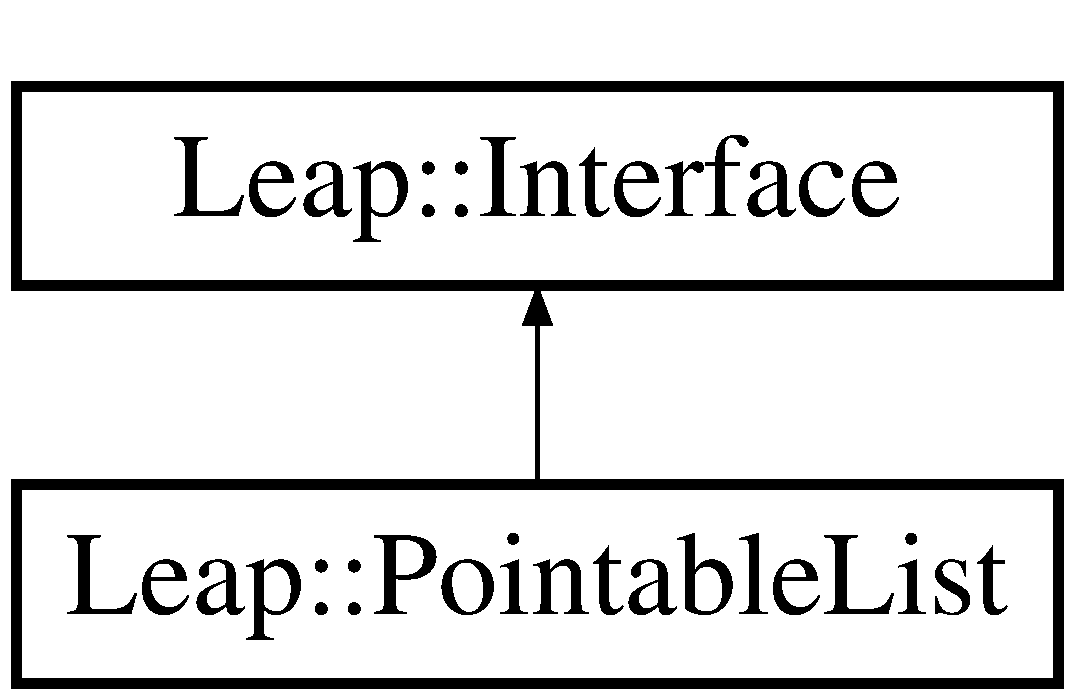
\includegraphics[height=2.000000cm]{class_leap_1_1_pointable_list}
\end{center}
\end{figure}
\subsection*{Public Types}
\begin{DoxyCompactItemize}
\item 
typedef \hyperlink{class_leap_1_1_const_list_iterator}{Const\+List\+Iterator}\\*
$<$ \hyperlink{class_leap_1_1_pointable_list}{Pointable\+List}, \hyperlink{class_leap_1_1_pointable}{Pointable} $>$ \hyperlink{class_leap_1_1_pointable_list_a12b640b8c7e70885884a3a6ee903c21c}{const\+\_\+iterator}
\end{DoxyCompactItemize}
\subsection*{Public Member Functions}
\begin{DoxyCompactItemize}
\item 
\hypertarget{class_leap_1_1_pointable_list_afeeb15c12648df910dbd27c120b4b649}{{\bfseries Pointable\+List} (const \hyperlink{class_leap_1_1_list_base_implementation}{List\+Base\+Implementation}$<$ \hyperlink{class_leap_1_1_pointable}{Pointable} $>$ \&)}\label{class_leap_1_1_pointable_list_afeeb15c12648df910dbd27c120b4b649}

\item 
L\+E\+A\+P\+\_\+\+E\+X\+P\+O\+R\+T \hyperlink{class_leap_1_1_pointable_list_ad8ba234f2a9491dd9c1062432e40ebf5}{Pointable\+List} ()
\item 
L\+E\+A\+P\+\_\+\+E\+X\+P\+O\+R\+T int \hyperlink{class_leap_1_1_pointable_list_a3a8aabe61fd964c0b60d18b743670c54}{count} () const 
\item 
L\+E\+A\+P\+\_\+\+E\+X\+P\+O\+R\+T bool \hyperlink{class_leap_1_1_pointable_list_aed63f1f0bb19495698686364f169c131}{is\+Empty} () const 
\item 
L\+E\+A\+P\+\_\+\+E\+X\+P\+O\+R\+T \hyperlink{class_leap_1_1_pointable}{Pointable} \hyperlink{class_leap_1_1_pointable_list_a2a0e9f1b2789028c7d958ecc197ced22}{operator\mbox{[}$\,$\mbox{]}} (int index) const 
\item 
L\+E\+A\+P\+\_\+\+E\+X\+P\+O\+R\+T \hyperlink{class_leap_1_1_pointable_list}{Pointable\+List} \& \hyperlink{class_leap_1_1_pointable_list_a415fee35b60e79f69a440096d6818d75}{append} (const \hyperlink{class_leap_1_1_pointable_list}{Pointable\+List} \&other)
\item 
L\+E\+A\+P\+\_\+\+E\+X\+P\+O\+R\+T \hyperlink{class_leap_1_1_pointable_list}{Pointable\+List} \& \hyperlink{class_leap_1_1_pointable_list_a8da39b0c202e3ade7aad666dcceddfdf}{append} (const \hyperlink{class_leap_1_1_finger_list}{Finger\+List} \&other)
\item 
L\+E\+A\+P\+\_\+\+E\+X\+P\+O\+R\+T \hyperlink{class_leap_1_1_pointable_list}{Pointable\+List} \& \hyperlink{class_leap_1_1_pointable_list_a091f0c1a7030f5f91701dd54f73a98de}{append} (const \hyperlink{class_leap_1_1_tool_list}{Tool\+List} \&other)
\item 
L\+E\+A\+P\+\_\+\+E\+X\+P\+O\+R\+T \hyperlink{class_leap_1_1_pointable}{Pointable} \hyperlink{class_leap_1_1_pointable_list_a769d774ccf140e4b597f9d03c64ade09}{leftmost} () const 
\item 
L\+E\+A\+P\+\_\+\+E\+X\+P\+O\+R\+T \hyperlink{class_leap_1_1_pointable}{Pointable} \hyperlink{class_leap_1_1_pointable_list_a9c5a12d32479519c7319c220b12dbfc5}{rightmost} () const 
\item 
L\+E\+A\+P\+\_\+\+E\+X\+P\+O\+R\+T \hyperlink{class_leap_1_1_pointable}{Pointable} \hyperlink{class_leap_1_1_pointable_list_afba3b5c70ce4b4939498b62f7cf7b9ba}{frontmost} () const 
\item 
L\+E\+A\+P\+\_\+\+E\+X\+P\+O\+R\+T \hyperlink{class_leap_1_1_pointable_list_a12b640b8c7e70885884a3a6ee903c21c}{const\+\_\+iterator} \hyperlink{class_leap_1_1_pointable_list_ae655d2e1fe70d0a15aab2da083e7f712}{begin} () const 
\item 
L\+E\+A\+P\+\_\+\+E\+X\+P\+O\+R\+T \hyperlink{class_leap_1_1_pointable_list_a12b640b8c7e70885884a3a6ee903c21c}{const\+\_\+iterator} \hyperlink{class_leap_1_1_pointable_list_a4dbbb5bcc6f3db906b3693ddc2aa3d6e}{end} () const 
\end{DoxyCompactItemize}
\subsection*{Additional Inherited Members}


\subsection{Detailed Description}
The \hyperlink{class_leap_1_1_pointable_list}{Pointable\+List} class represents a list of \hyperlink{class_leap_1_1_pointable}{Pointable} objects.

\hyperlink{class_leap_1_1_pointable}{Pointable} objects include entities that can be pointed, such as fingers and tools.

Get a \hyperlink{class_leap_1_1_pointable_list}{Pointable\+List} object by calling \hyperlink{class_leap_1_1_frame_a1bc989343a3b971568368c77b5869fb9}{Frame\+::pointables()}. \begin{DoxySince}{Since}
1.\+0 
\end{DoxySince}


\subsection{Member Typedef Documentation}
\hypertarget{class_leap_1_1_pointable_list_a12b640b8c7e70885884a3a6ee903c21c}{\index{Leap\+::\+Pointable\+List@{Leap\+::\+Pointable\+List}!const\+\_\+iterator@{const\+\_\+iterator}}
\index{const\+\_\+iterator@{const\+\_\+iterator}!Leap\+::\+Pointable\+List@{Leap\+::\+Pointable\+List}}
\subsubsection[{const\+\_\+iterator}]{\setlength{\rightskip}{0pt plus 5cm}typedef {\bf Const\+List\+Iterator}$<${\bf Pointable\+List}, {\bf Pointable}$>$ {\bf Leap\+::\+Pointable\+List\+::const\+\_\+iterator}}}\label{class_leap_1_1_pointable_list_a12b640b8c7e70885884a3a6ee903c21c}
A C++ iterator type for \hyperlink{class_leap_1_1_pointable_list}{Pointable\+List} objects. \begin{DoxySince}{Since}
1.\+0 
\end{DoxySince}


\subsection{Constructor \& Destructor Documentation}
\hypertarget{class_leap_1_1_pointable_list_ad8ba234f2a9491dd9c1062432e40ebf5}{\index{Leap\+::\+Pointable\+List@{Leap\+::\+Pointable\+List}!Pointable\+List@{Pointable\+List}}
\index{Pointable\+List@{Pointable\+List}!Leap\+::\+Pointable\+List@{Leap\+::\+Pointable\+List}}
\subsubsection[{Pointable\+List}]{\setlength{\rightskip}{0pt plus 5cm}L\+E\+A\+P\+\_\+\+E\+X\+P\+O\+R\+T Leap\+::\+Pointable\+List\+::\+Pointable\+List (
\begin{DoxyParamCaption}
{}
\end{DoxyParamCaption}
)}}\label{class_leap_1_1_pointable_list_ad8ba234f2a9491dd9c1062432e40ebf5}
Constructs an empty list of pointable entities. \begin{DoxySince}{Since}
1.\+0 
\end{DoxySince}


\subsection{Member Function Documentation}
\hypertarget{class_leap_1_1_pointable_list_a415fee35b60e79f69a440096d6818d75}{\index{Leap\+::\+Pointable\+List@{Leap\+::\+Pointable\+List}!append@{append}}
\index{append@{append}!Leap\+::\+Pointable\+List@{Leap\+::\+Pointable\+List}}
\subsubsection[{append}]{\setlength{\rightskip}{0pt plus 5cm}L\+E\+A\+P\+\_\+\+E\+X\+P\+O\+R\+T {\bf Pointable\+List}\& Leap\+::\+Pointable\+List\+::append (
\begin{DoxyParamCaption}
\item[{const {\bf Pointable\+List} \&}]{other}
\end{DoxyParamCaption}
)}}\label{class_leap_1_1_pointable_list_a415fee35b60e79f69a440096d6818d75}
Appends the members of the specifed \hyperlink{class_leap_1_1_pointable_list}{Pointable\+List} to this \hyperlink{class_leap_1_1_pointable_list}{Pointable\+List}. 
\begin{DoxyParams}{Parameters}
{\em other} & A \hyperlink{class_leap_1_1_pointable_list}{Pointable\+List} object containing \hyperlink{class_leap_1_1_pointable}{Pointable} objects to append to the end of this \hyperlink{class_leap_1_1_pointable_list}{Pointable\+List}. \\
\hline
\end{DoxyParams}
\begin{DoxySince}{Since}
1.\+0 
\end{DoxySince}
\hypertarget{class_leap_1_1_pointable_list_a8da39b0c202e3ade7aad666dcceddfdf}{\index{Leap\+::\+Pointable\+List@{Leap\+::\+Pointable\+List}!append@{append}}
\index{append@{append}!Leap\+::\+Pointable\+List@{Leap\+::\+Pointable\+List}}
\subsubsection[{append}]{\setlength{\rightskip}{0pt plus 5cm}L\+E\+A\+P\+\_\+\+E\+X\+P\+O\+R\+T {\bf Pointable\+List}\& Leap\+::\+Pointable\+List\+::append (
\begin{DoxyParamCaption}
\item[{const {\bf Finger\+List} \&}]{other}
\end{DoxyParamCaption}
)}}\label{class_leap_1_1_pointable_list_a8da39b0c202e3ade7aad666dcceddfdf}
Appends the members of the specifed \hyperlink{class_leap_1_1_finger_list}{Finger\+List} to this \hyperlink{class_leap_1_1_pointable_list}{Pointable\+List}. 
\begin{DoxyParams}{Parameters}
{\em other} & A \hyperlink{class_leap_1_1_finger_list}{Finger\+List} object containing \hyperlink{class_leap_1_1_finger}{Finger} objects to append to the end of this \hyperlink{class_leap_1_1_pointable_list}{Pointable\+List}. \\
\hline
\end{DoxyParams}
\begin{DoxySince}{Since}
1.\+0 
\end{DoxySince}
\hypertarget{class_leap_1_1_pointable_list_a091f0c1a7030f5f91701dd54f73a98de}{\index{Leap\+::\+Pointable\+List@{Leap\+::\+Pointable\+List}!append@{append}}
\index{append@{append}!Leap\+::\+Pointable\+List@{Leap\+::\+Pointable\+List}}
\subsubsection[{append}]{\setlength{\rightskip}{0pt plus 5cm}L\+E\+A\+P\+\_\+\+E\+X\+P\+O\+R\+T {\bf Pointable\+List}\& Leap\+::\+Pointable\+List\+::append (
\begin{DoxyParamCaption}
\item[{const {\bf Tool\+List} \&}]{other}
\end{DoxyParamCaption}
)}}\label{class_leap_1_1_pointable_list_a091f0c1a7030f5f91701dd54f73a98de}
Appends the members of the specifed \hyperlink{class_leap_1_1_tool_list}{Tool\+List} to this \hyperlink{class_leap_1_1_pointable_list}{Pointable\+List}. 
\begin{DoxyParams}{Parameters}
{\em other} & A \hyperlink{class_leap_1_1_tool_list}{Tool\+List} object containing \hyperlink{class_leap_1_1_tool}{Tool} objects to append to the end of this \hyperlink{class_leap_1_1_pointable_list}{Pointable\+List}. \\
\hline
\end{DoxyParams}
\begin{DoxySince}{Since}
1.\+0 
\end{DoxySince}
\hypertarget{class_leap_1_1_pointable_list_ae655d2e1fe70d0a15aab2da083e7f712}{\index{Leap\+::\+Pointable\+List@{Leap\+::\+Pointable\+List}!begin@{begin}}
\index{begin@{begin}!Leap\+::\+Pointable\+List@{Leap\+::\+Pointable\+List}}
\subsubsection[{begin}]{\setlength{\rightskip}{0pt plus 5cm}L\+E\+A\+P\+\_\+\+E\+X\+P\+O\+R\+T {\bf const\+\_\+iterator} Leap\+::\+Pointable\+List\+::begin (
\begin{DoxyParamCaption}
{}
\end{DoxyParamCaption}
) const}}\label{class_leap_1_1_pointable_list_ae655d2e1fe70d0a15aab2da083e7f712}
The C++ iterator set to the beginning of this \hyperlink{class_leap_1_1_pointable_list}{Pointable\+List}. \begin{DoxySince}{Since}
1.\+0 
\end{DoxySince}
\hypertarget{class_leap_1_1_pointable_list_a3a8aabe61fd964c0b60d18b743670c54}{\index{Leap\+::\+Pointable\+List@{Leap\+::\+Pointable\+List}!count@{count}}
\index{count@{count}!Leap\+::\+Pointable\+List@{Leap\+::\+Pointable\+List}}
\subsubsection[{count}]{\setlength{\rightskip}{0pt plus 5cm}L\+E\+A\+P\+\_\+\+E\+X\+P\+O\+R\+T int Leap\+::\+Pointable\+List\+::count (
\begin{DoxyParamCaption}
{}
\end{DoxyParamCaption}
) const}}\label{class_leap_1_1_pointable_list_a3a8aabe61fd964c0b60d18b743670c54}
Returns the number of pointable entities in this list. \begin{DoxyReturn}{Returns}
The number of pointable entities in this list. 
\end{DoxyReturn}
\begin{DoxySince}{Since}
1.\+0 
\end{DoxySince}
\hypertarget{class_leap_1_1_pointable_list_a4dbbb5bcc6f3db906b3693ddc2aa3d6e}{\index{Leap\+::\+Pointable\+List@{Leap\+::\+Pointable\+List}!end@{end}}
\index{end@{end}!Leap\+::\+Pointable\+List@{Leap\+::\+Pointable\+List}}
\subsubsection[{end}]{\setlength{\rightskip}{0pt plus 5cm}L\+E\+A\+P\+\_\+\+E\+X\+P\+O\+R\+T {\bf const\+\_\+iterator} Leap\+::\+Pointable\+List\+::end (
\begin{DoxyParamCaption}
{}
\end{DoxyParamCaption}
) const}}\label{class_leap_1_1_pointable_list_a4dbbb5bcc6f3db906b3693ddc2aa3d6e}
The C++ iterator set to the end of this \hyperlink{class_leap_1_1_pointable_list}{Pointable\+List}. \begin{DoxySince}{Since}
1.\+0 
\end{DoxySince}
\hypertarget{class_leap_1_1_pointable_list_afba3b5c70ce4b4939498b62f7cf7b9ba}{\index{Leap\+::\+Pointable\+List@{Leap\+::\+Pointable\+List}!frontmost@{frontmost}}
\index{frontmost@{frontmost}!Leap\+::\+Pointable\+List@{Leap\+::\+Pointable\+List}}
\subsubsection[{frontmost}]{\setlength{\rightskip}{0pt plus 5cm}L\+E\+A\+P\+\_\+\+E\+X\+P\+O\+R\+T {\bf Pointable} Leap\+::\+Pointable\+List\+::frontmost (
\begin{DoxyParamCaption}
{}
\end{DoxyParamCaption}
) const}}\label{class_leap_1_1_pointable_list_afba3b5c70ce4b4939498b62f7cf7b9ba}
The member of the list that is farthest to the front within the standard Leap Motion frame of reference (i.\+e has the smallest Z coordinate).

\begin{DoxyReturn}{Returns}
The frontmost pointable, or invalid if list is empty. 
\end{DoxyReturn}
\begin{DoxySince}{Since}
1.\+0 
\end{DoxySince}
\hypertarget{class_leap_1_1_pointable_list_aed63f1f0bb19495698686364f169c131}{\index{Leap\+::\+Pointable\+List@{Leap\+::\+Pointable\+List}!is\+Empty@{is\+Empty}}
\index{is\+Empty@{is\+Empty}!Leap\+::\+Pointable\+List@{Leap\+::\+Pointable\+List}}
\subsubsection[{is\+Empty}]{\setlength{\rightskip}{0pt plus 5cm}L\+E\+A\+P\+\_\+\+E\+X\+P\+O\+R\+T bool Leap\+::\+Pointable\+List\+::is\+Empty (
\begin{DoxyParamCaption}
{}
\end{DoxyParamCaption}
) const}}\label{class_leap_1_1_pointable_list_aed63f1f0bb19495698686364f169c131}
Reports whether the list is empty. \begin{DoxyReturn}{Returns}
True, if the list has no members. 
\end{DoxyReturn}
\begin{DoxySince}{Since}
1.\+0 
\end{DoxySince}
\hypertarget{class_leap_1_1_pointable_list_a769d774ccf140e4b597f9d03c64ade09}{\index{Leap\+::\+Pointable\+List@{Leap\+::\+Pointable\+List}!leftmost@{leftmost}}
\index{leftmost@{leftmost}!Leap\+::\+Pointable\+List@{Leap\+::\+Pointable\+List}}
\subsubsection[{leftmost}]{\setlength{\rightskip}{0pt plus 5cm}L\+E\+A\+P\+\_\+\+E\+X\+P\+O\+R\+T {\bf Pointable} Leap\+::\+Pointable\+List\+::leftmost (
\begin{DoxyParamCaption}
{}
\end{DoxyParamCaption}
) const}}\label{class_leap_1_1_pointable_list_a769d774ccf140e4b597f9d03c64ade09}
The member of the list that is farthest to the left within the standard Leap Motion frame of reference (i.\+e has the smallest X coordinate).

\begin{DoxyReturn}{Returns}
The leftmost pointable, or invalid if list is empty. 
\end{DoxyReturn}
\begin{DoxySince}{Since}
1.\+0 
\end{DoxySince}
\hypertarget{class_leap_1_1_pointable_list_a2a0e9f1b2789028c7d958ecc197ced22}{\index{Leap\+::\+Pointable\+List@{Leap\+::\+Pointable\+List}!operator\mbox{[}$\,$\mbox{]}@{operator[]}}
\index{operator\mbox{[}$\,$\mbox{]}@{operator[]}!Leap\+::\+Pointable\+List@{Leap\+::\+Pointable\+List}}
\subsubsection[{operator[]}]{\setlength{\rightskip}{0pt plus 5cm}L\+E\+A\+P\+\_\+\+E\+X\+P\+O\+R\+T {\bf Pointable} Leap\+::\+Pointable\+List\+::operator\mbox{[}$\,$\mbox{]} (
\begin{DoxyParamCaption}
\item[{int}]{index}
\end{DoxyParamCaption}
) const}}\label{class_leap_1_1_pointable_list_a2a0e9f1b2789028c7d958ecc197ced22}
Access a list member by its position in the list. 
\begin{DoxyParams}{Parameters}
{\em index} & The zero-\/based list position index. \\
\hline
\end{DoxyParams}
\begin{DoxyReturn}{Returns}
The \hyperlink{class_leap_1_1_pointable}{Pointable} object at the specified index. 
\end{DoxyReturn}
\begin{DoxySince}{Since}
1.\+0 
\end{DoxySince}
\hypertarget{class_leap_1_1_pointable_list_a9c5a12d32479519c7319c220b12dbfc5}{\index{Leap\+::\+Pointable\+List@{Leap\+::\+Pointable\+List}!rightmost@{rightmost}}
\index{rightmost@{rightmost}!Leap\+::\+Pointable\+List@{Leap\+::\+Pointable\+List}}
\subsubsection[{rightmost}]{\setlength{\rightskip}{0pt plus 5cm}L\+E\+A\+P\+\_\+\+E\+X\+P\+O\+R\+T {\bf Pointable} Leap\+::\+Pointable\+List\+::rightmost (
\begin{DoxyParamCaption}
{}
\end{DoxyParamCaption}
) const}}\label{class_leap_1_1_pointable_list_a9c5a12d32479519c7319c220b12dbfc5}
The member of the list that is farthest to the right within the standard Leap Motion frame of reference (i.\+e has the largest X coordinate).

\begin{DoxyReturn}{Returns}
The rightmost pointable, or invalid if list is empty. 
\end{DoxyReturn}
\begin{DoxySince}{Since}
1.\+0 
\end{DoxySince}


The documentation for this class was generated from the following file\+:\begin{DoxyCompactItemize}
\item 
Interface\+Managers/Leap.\+h\end{DoxyCompactItemize}

\hypertarget{class_leap_1_1_screen}{\section{Leap\+:\+:Screen Class Reference}
\label{class_leap_1_1_screen}\index{Leap\+::\+Screen@{Leap\+::\+Screen}}
}


{\ttfamily \#include $<$Leap.\+h$>$}

Inheritance diagram for Leap\+:\+:Screen\+:\begin{figure}[H]
\begin{center}
\leavevmode
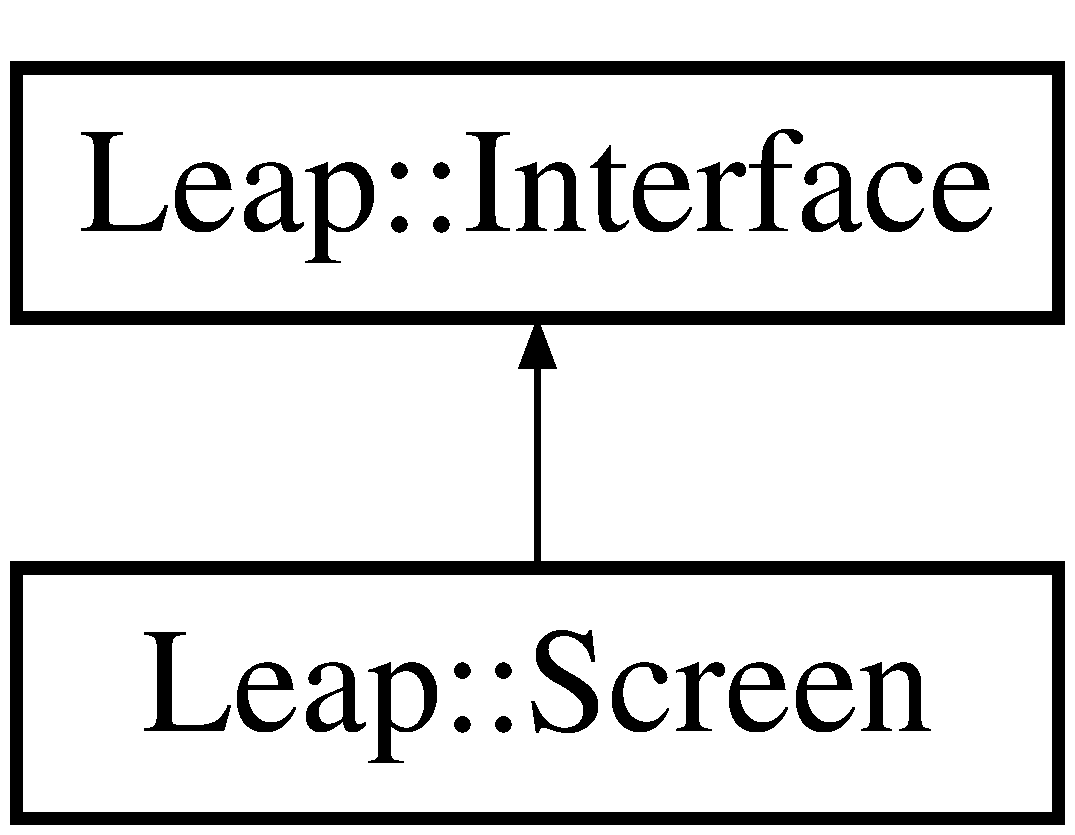
\includegraphics[height=2.000000cm]{class_leap_1_1_screen}
\end{center}
\end{figure}
\subsection*{Public Member Functions}
\begin{DoxyCompactItemize}
\item 
\hypertarget{class_leap_1_1_screen_ae4bacceec22fd48fa983f863854a1442}{{\bfseries Screen} (Screen\+Implementation $\ast$)}\label{class_leap_1_1_screen_ae4bacceec22fd48fa983f863854a1442}

\item 
L\+E\+A\+P\+\_\+\+E\+X\+P\+O\+R\+T \hyperlink{class_leap_1_1_screen_a65dcdd83ed5edb4f6e19a9a40edcb96f}{Screen} ()
\item 
L\+E\+A\+P\+\_\+\+E\+X\+P\+O\+R\+T int32\+\_\+t \hyperlink{class_leap_1_1_screen_ae209881171841c1c172b582640e5c31c}{id} () const 
\item 
L\+E\+A\+P\+\_\+\+E\+X\+P\+O\+R\+T \hyperlink{struct_leap_1_1_vector}{Vector} \hyperlink{class_leap_1_1_screen_a4264a354488a387ab5657c73d594b41a}{intersect} (const \hyperlink{class_leap_1_1_pointable}{Pointable} \&pointable, bool normalize, float clamp\+Ratio=1.\+0f) const 
\item 
L\+E\+A\+P\+\_\+\+E\+X\+P\+O\+R\+T \hyperlink{struct_leap_1_1_vector}{Vector} \hyperlink{class_leap_1_1_screen_af7f4942267686be891f371feff54edd2}{intersect} (const \hyperlink{struct_leap_1_1_vector}{Vector} \&position, const \hyperlink{struct_leap_1_1_vector}{Vector} \&direction, bool normalize, float clamp\+Ratio=1.\+0f) const 
\item 
L\+E\+A\+P\+\_\+\+E\+X\+P\+O\+R\+T \hyperlink{struct_leap_1_1_vector}{Vector} \hyperlink{class_leap_1_1_screen_a5ac637faf6b1c296ce3289265ecb359d}{project} (const \hyperlink{struct_leap_1_1_vector}{Vector} \&position, bool normalize, float clamp\+Ratio=1.\+0f) const 
\item 
L\+E\+A\+P\+\_\+\+E\+X\+P\+O\+R\+T \hyperlink{struct_leap_1_1_vector}{Vector} \hyperlink{class_leap_1_1_screen_aa6007a37823a83b7620256037337e7f3}{horizontal\+Axis} () const 
\item 
L\+E\+A\+P\+\_\+\+E\+X\+P\+O\+R\+T \hyperlink{struct_leap_1_1_vector}{Vector} \hyperlink{class_leap_1_1_screen_a195e300396f259a01a9115ce18bf66da}{vertical\+Axis} () const 
\item 
L\+E\+A\+P\+\_\+\+E\+X\+P\+O\+R\+T \hyperlink{struct_leap_1_1_vector}{Vector} \hyperlink{class_leap_1_1_screen_a617b14ae37341969a59a5f99cae61ac4}{bottom\+Left\+Corner} () const 
\item 
L\+E\+A\+P\+\_\+\+E\+X\+P\+O\+R\+T \hyperlink{struct_leap_1_1_vector}{Vector} \hyperlink{class_leap_1_1_screen_a3cf3c55d32dc11b097d1dbdd14e1ee1d}{normal} () const 
\item 
L\+E\+A\+P\+\_\+\+E\+X\+P\+O\+R\+T int \hyperlink{class_leap_1_1_screen_a183e75cf160db9dfa9653c0f128adac0}{width\+Pixels} () const 
\item 
L\+E\+A\+P\+\_\+\+E\+X\+P\+O\+R\+T int \hyperlink{class_leap_1_1_screen_a73ec00f33fe7aee01e2a63de06311d79}{height\+Pixels} () const 
\item 
L\+E\+A\+P\+\_\+\+E\+X\+P\+O\+R\+T float \hyperlink{class_leap_1_1_screen_a0eeef9ff9931be5d9d9b34f0b0068e40}{distance\+To\+Point} (const \hyperlink{struct_leap_1_1_vector}{Vector} \&point) const 
\item 
L\+E\+A\+P\+\_\+\+E\+X\+P\+O\+R\+T bool \hyperlink{class_leap_1_1_screen_aebb6c054d2b35e27b8991618945ec614}{is\+Valid} () const 
\item 
L\+E\+A\+P\+\_\+\+E\+X\+P\+O\+R\+T bool \hyperlink{class_leap_1_1_screen_a874b0b7326974a98d832a368cf9d815a}{operator==} (const \hyperlink{class_leap_1_1_screen}{Screen} \&) const 
\item 
L\+E\+A\+P\+\_\+\+E\+X\+P\+O\+R\+T bool \hyperlink{class_leap_1_1_screen_a7767f6df72c0ab3daecdef5960061ad8}{operator!=} (const \hyperlink{class_leap_1_1_screen}{Screen} \&) const 
\item 
L\+E\+A\+P\+\_\+\+E\+X\+P\+O\+R\+T std\+::string \hyperlink{class_leap_1_1_screen_a6215a10c9948f75522d2932b6b91b35c}{to\+String} () const 
\end{DoxyCompactItemize}
\subsection*{Static Public Member Functions}
\begin{DoxyCompactItemize}
\item 
static L\+E\+A\+P\+\_\+\+E\+X\+P\+O\+R\+T const \hyperlink{class_leap_1_1_screen}{Screen} \& \hyperlink{class_leap_1_1_screen_a380e39a87c63fd4915f1f5e5c5db0c3c}{invalid} ()
\end{DoxyCompactItemize}
\subsection*{Friends}
\begin{DoxyCompactItemize}
\item 
L\+E\+A\+P\+\_\+\+E\+X\+P\+O\+R\+T friend std\+::ostream \& \hyperlink{class_leap_1_1_screen_a9d392849d557b2c5107a836a227d63a6}{operator$<$$<$} (std\+::ostream \&, const \hyperlink{class_leap_1_1_screen}{Screen} \&)
\end{DoxyCompactItemize}
\subsection*{Additional Inherited Members}


\subsection{Detailed Description}
The \hyperlink{class_leap_1_1_screen}{Screen} class represents a computer monitor screen.

The \hyperlink{class_leap_1_1_screen}{Screen} class reports characteristics describing the position and orientation of the monitor screen within the Leap Motion coordinate system. These characteristics include the bottom-\/left corner position of the screen, direction vectors for the horizontal and vertical axes of the screen, and the screen's normal vector. The screen must be properly registered with the \hyperlink{class_leap_1_1_screen}{Screen} Locator for the Leap Motion software to report these characteristics accurately. The \hyperlink{class_leap_1_1_screen}{Screen} class also reports the size of the screen in pixels, using information obtained from the operating system. (Run the \hyperlink{class_leap_1_1_screen}{Screen} Locator from the Leap Motion Settings dialog, on the \hyperlink{class_leap_1_1_screen}{Screen} page.)

You can get the point of intersection between the screen and a ray projected from a \hyperlink{class_leap_1_1_pointable}{Pointable} object using the \hyperlink{class_leap_1_1_screen_a4264a354488a387ab5657c73d594b41a}{Screen\+::intersect()} function. Likewise, you can get the closest point on the screen to a point in space using the \hyperlink{class_leap_1_1_screen_a5ac637faf6b1c296ce3289265ecb359d}{Screen\+::project()} function. Again, the screen location must be registered with the \hyperlink{class_leap_1_1_screen}{Screen} Locator for these functions to return accurate values.

Note that \hyperlink{class_leap_1_1_screen}{Screen} objects can be invalid, which means that they do not contain valid screen coordinate data and do not correspond to a physical entity. Test for validity with the \hyperlink{class_leap_1_1_screen_aebb6c054d2b35e27b8991618945ec614}{Screen\+::is\+Valid()} function. \begin{DoxySince}{Since}
1.\+0 
\end{DoxySince}


\subsection{Constructor \& Destructor Documentation}
\hypertarget{class_leap_1_1_screen_a65dcdd83ed5edb4f6e19a9a40edcb96f}{\index{Leap\+::\+Screen@{Leap\+::\+Screen}!Screen@{Screen}}
\index{Screen@{Screen}!Leap\+::\+Screen@{Leap\+::\+Screen}}
\subsubsection[{Screen}]{\setlength{\rightskip}{0pt plus 5cm}L\+E\+A\+P\+\_\+\+E\+X\+P\+O\+R\+T Leap\+::\+Screen\+::\+Screen (
\begin{DoxyParamCaption}
{}
\end{DoxyParamCaption}
)}}\label{class_leap_1_1_screen_a65dcdd83ed5edb4f6e19a9a40edcb96f}
Constructs a \hyperlink{class_leap_1_1_screen}{Screen} object.

An uninitialized screen is considered invalid. Get valid \hyperlink{class_leap_1_1_screen}{Screen} objects from a \hyperlink{class_leap_1_1_screen_list}{Screen\+List} object obtained using the \hyperlink{class_leap_1_1_controller_ab6cf5b48ef434b3d58cf8962451f4df3}{Controller\+::located\+Screens()} method. \begin{DoxySince}{Since}
1.\+0 
\end{DoxySince}


\subsection{Member Function Documentation}
\hypertarget{class_leap_1_1_screen_a617b14ae37341969a59a5f99cae61ac4}{\index{Leap\+::\+Screen@{Leap\+::\+Screen}!bottom\+Left\+Corner@{bottom\+Left\+Corner}}
\index{bottom\+Left\+Corner@{bottom\+Left\+Corner}!Leap\+::\+Screen@{Leap\+::\+Screen}}
\subsubsection[{bottom\+Left\+Corner}]{\setlength{\rightskip}{0pt plus 5cm}L\+E\+A\+P\+\_\+\+E\+X\+P\+O\+R\+T {\bf Vector} Leap\+::\+Screen\+::bottom\+Left\+Corner (
\begin{DoxyParamCaption}
{}
\end{DoxyParamCaption}
) const}}\label{class_leap_1_1_screen_a617b14ae37341969a59a5f99cae61ac4}
A \hyperlink{struct_leap_1_1_vector}{Vector} representing the bottom left corner of this \hyperlink{class_leap_1_1_screen}{Screen} within the Leap Motion coordinate system.

The point represented by this vector defines the origin of the screen in the Leap Motion coordinate system.

Together, \hyperlink{class_leap_1_1_screen_aa6007a37823a83b7620256037337e7f3}{horizontal\+Axis()}, \hyperlink{class_leap_1_1_screen_a195e300396f259a01a9115ce18bf66da}{vertical\+Axis()}, and \hyperlink{class_leap_1_1_screen_a617b14ae37341969a59a5f99cae61ac4}{bottom\+Left\+Corner()} describe the physical position, size and orientation of this \hyperlink{class_leap_1_1_screen}{Screen}.

\begin{DoxyReturn}{Returns}
A \hyperlink{struct_leap_1_1_vector}{Vector} containing the coordinates of the bottom-\/left corner of this \hyperlink{class_leap_1_1_screen}{Screen}. 
\end{DoxyReturn}
\begin{DoxySince}{Since}
1.\+0 
\end{DoxySince}
\hypertarget{class_leap_1_1_screen_a0eeef9ff9931be5d9d9b34f0b0068e40}{\index{Leap\+::\+Screen@{Leap\+::\+Screen}!distance\+To\+Point@{distance\+To\+Point}}
\index{distance\+To\+Point@{distance\+To\+Point}!Leap\+::\+Screen@{Leap\+::\+Screen}}
\subsubsection[{distance\+To\+Point}]{\setlength{\rightskip}{0pt plus 5cm}L\+E\+A\+P\+\_\+\+E\+X\+P\+O\+R\+T float Leap\+::\+Screen\+::distance\+To\+Point (
\begin{DoxyParamCaption}
\item[{const {\bf Vector} \&}]{point}
\end{DoxyParamCaption}
) const}}\label{class_leap_1_1_screen_a0eeef9ff9931be5d9d9b34f0b0068e40}
The shortest distance from the specified point to the plane in which this \hyperlink{class_leap_1_1_screen}{Screen} lies.

\begin{DoxyReturn}{Returns}
The length of the perpendicular line segment extending from the plane this \hyperlink{class_leap_1_1_screen}{Screen} lies in to the specified point. 
\end{DoxyReturn}
\begin{DoxySince}{Since}
1.\+0 
\end{DoxySince}
\hypertarget{class_leap_1_1_screen_a73ec00f33fe7aee01e2a63de06311d79}{\index{Leap\+::\+Screen@{Leap\+::\+Screen}!height\+Pixels@{height\+Pixels}}
\index{height\+Pixels@{height\+Pixels}!Leap\+::\+Screen@{Leap\+::\+Screen}}
\subsubsection[{height\+Pixels}]{\setlength{\rightskip}{0pt plus 5cm}L\+E\+A\+P\+\_\+\+E\+X\+P\+O\+R\+T int Leap\+::\+Screen\+::height\+Pixels (
\begin{DoxyParamCaption}
{}
\end{DoxyParamCaption}
) const}}\label{class_leap_1_1_screen_a73ec00f33fe7aee01e2a63de06311d79}
The vertical resolution of this screen, in pixels.

\begin{DoxyReturn}{Returns}
The height of this \hyperlink{class_leap_1_1_screen}{Screen} in pixels. 
\end{DoxyReturn}
\begin{DoxySince}{Since}
1.\+0 
\end{DoxySince}
\hypertarget{class_leap_1_1_screen_aa6007a37823a83b7620256037337e7f3}{\index{Leap\+::\+Screen@{Leap\+::\+Screen}!horizontal\+Axis@{horizontal\+Axis}}
\index{horizontal\+Axis@{horizontal\+Axis}!Leap\+::\+Screen@{Leap\+::\+Screen}}
\subsubsection[{horizontal\+Axis}]{\setlength{\rightskip}{0pt plus 5cm}L\+E\+A\+P\+\_\+\+E\+X\+P\+O\+R\+T {\bf Vector} Leap\+::\+Screen\+::horizontal\+Axis (
\begin{DoxyParamCaption}
{}
\end{DoxyParamCaption}
) const}}\label{class_leap_1_1_screen_aa6007a37823a83b7620256037337e7f3}
A \hyperlink{struct_leap_1_1_vector}{Vector} representing the horizontal axis of this \hyperlink{class_leap_1_1_screen}{Screen} within the Leap Motion coordinate system.

The magnitude of this vector estimates the physical width of this \hyperlink{class_leap_1_1_screen}{Screen} in millimeters. The direction of this vector is parallel to the bottom edge of the screen and points toward the right edge of the screen.

Together, \hyperlink{class_leap_1_1_screen_aa6007a37823a83b7620256037337e7f3}{horizontal\+Axis()}, \hyperlink{class_leap_1_1_screen_a195e300396f259a01a9115ce18bf66da}{vertical\+Axis()}, and \hyperlink{class_leap_1_1_screen_a617b14ae37341969a59a5f99cae61ac4}{bottom\+Left\+Corner()} describe the physical position, size and orientation of this \hyperlink{class_leap_1_1_screen}{Screen}.

\begin{DoxyReturn}{Returns}
A \hyperlink{struct_leap_1_1_vector}{Vector} representing the bottom, horizontal edge of this \hyperlink{class_leap_1_1_screen}{Screen}. 
\end{DoxyReturn}
\begin{DoxySince}{Since}
1.\+0 
\end{DoxySince}
\hypertarget{class_leap_1_1_screen_ae209881171841c1c172b582640e5c31c}{\index{Leap\+::\+Screen@{Leap\+::\+Screen}!id@{id}}
\index{id@{id}!Leap\+::\+Screen@{Leap\+::\+Screen}}
\subsubsection[{id}]{\setlength{\rightskip}{0pt plus 5cm}L\+E\+A\+P\+\_\+\+E\+X\+P\+O\+R\+T int32\+\_\+t Leap\+::\+Screen\+::id (
\begin{DoxyParamCaption}
{}
\end{DoxyParamCaption}
) const}}\label{class_leap_1_1_screen_ae209881171841c1c172b582640e5c31c}
A unique identifier for this screen based on the screen information in the configuration. A default screen with I\+D, {\itshape 0}, always exists and contains default characteristics, even if no screens have been located. \begin{DoxySince}{Since}
1.\+0 
\end{DoxySince}
\hypertarget{class_leap_1_1_screen_a4264a354488a387ab5657c73d594b41a}{\index{Leap\+::\+Screen@{Leap\+::\+Screen}!intersect@{intersect}}
\index{intersect@{intersect}!Leap\+::\+Screen@{Leap\+::\+Screen}}
\subsubsection[{intersect}]{\setlength{\rightskip}{0pt plus 5cm}L\+E\+A\+P\+\_\+\+E\+X\+P\+O\+R\+T {\bf Vector} Leap\+::\+Screen\+::intersect (
\begin{DoxyParamCaption}
\item[{const {\bf Pointable} \&}]{pointable, }
\item[{bool}]{normalize, }
\item[{float}]{clamp\+Ratio = {\ttfamily 1.0f}}
\end{DoxyParamCaption}
) const}}\label{class_leap_1_1_screen_a4264a354488a387ab5657c73d594b41a}
Returns the intersection between this screen and a ray projecting from a \hyperlink{class_leap_1_1_pointable}{Pointable} object.

The projected ray emanates from the \hyperlink{class_leap_1_1_pointable}{Pointable} tip\+Position along the \hyperlink{class_leap_1_1_pointable}{Pointable}'s direction vector.

Set the normalize parameter to true to request the intersection point in normalized screen coordinates. Normalized screen coordinates are usually values between 0 and 1, where 0 represents the screen's origin at the bottom-\/left corner and 1 represents the opposite edge (either top or right). When you request normalized coordinates, the z-\/component of the returned vector is zero. Multiply a normalized coordinate by the values returned by \hyperlink{class_leap_1_1_screen_a183e75cf160db9dfa9653c0f128adac0}{Screen\+::width\+Pixels()} or \hyperlink{class_leap_1_1_screen_a73ec00f33fe7aee01e2a63de06311d79}{Screen\+::height\+Pixels()} to calculate the screen position in pixels (remembering that many other computer graphics coordinate systems place the origin in the top-\/left corner).

Set the normalize parameter to false to request the intersection point in Leap Motion coordinates (millimeters from the Leap Motion origin).

If the \hyperlink{class_leap_1_1_pointable}{Pointable} object points outside the screen's border (but still intersects the plane in which the screen lies), the returned intersection point is clamped to the nearest point on the edge of the screen.

You can use the clamp\+Ratio parameter to contract or expand the area in which you can point. For example, if you set the clamp\+Ratio parameter to 0.\+5, then the positions reported for intersection points outside the central 50\% of the screen are moved to the border of this smaller area. If, on the other hand, you expanded the area by setting clamp\+Ratio to a value such as 3.\+0, then you could point well outside screen's physical boundary before the intersection points would be clamped. The positions for any points clamped would also be placed on this larger outer border. The positions reported for any intersection points inside the clamping border are unaffected by clamping.


\begin{DoxyCodeInclude}
\end{DoxyCodeInclude}


If the \hyperlink{class_leap_1_1_pointable}{Pointable} object does not point toward the plane of the screen (i.\+e. it is pointing parallel to or away from the screen), then the components of the returned vector are all set to Na\+N (not-\/a-\/number).


\begin{DoxyParams}{Parameters}
{\em pointable} & The \hyperlink{class_leap_1_1_pointable}{Pointable} object to check for screen intersection.\\
\hline
{\em normalize} & If true, return normalized coordinates representing the intersection point as a percentage of the screen's width and height. If false, return Leap Motion coordinates (millimeters from the Leap Motion origin, which is located at the center of the top surface of the Leap Motion \hyperlink{class_leap_1_1_controller}{Controller}). If true and the clamp\+Ratio parameter is set to 1.\+0, coordinates will be of the form (0..1, 0..1, 0). Setting the clamp\+Ratio to a different value changes the range for normalized coordinates. For example, a clamp\+Ratio of 5.\+0 changes the range of values to be of the form (-\/2..3, -\/2..3, 0).\\
\hline
{\em clamp\+Ratio} & Adjusts the clamping border around this screen. By default this ratio is 1.\+0, and the border corresponds to the actual boundaries of the screen. Setting clamp\+Ratio to 0.\+5 would reduce the interaction area. Likewise, setting the ratio to 2.\+0 would increase the interaction area, adding 50\% around each edge of the physical monitor. Intersection points outside the interaction area are repositioned to the closest point on the clamping border before the vector is returned.\\
\hline
\end{DoxyParams}
\begin{DoxyReturn}{Returns}
A \hyperlink{struct_leap_1_1_vector}{Vector} containing the coordinates of the intersection between this screen and a ray projecting from the specified \hyperlink{class_leap_1_1_pointable}{Pointable} object. 
\end{DoxyReturn}
\begin{DoxySince}{Since}
1.\+0 
\end{DoxySince}
\hypertarget{class_leap_1_1_screen_af7f4942267686be891f371feff54edd2}{\index{Leap\+::\+Screen@{Leap\+::\+Screen}!intersect@{intersect}}
\index{intersect@{intersect}!Leap\+::\+Screen@{Leap\+::\+Screen}}
\subsubsection[{intersect}]{\setlength{\rightskip}{0pt plus 5cm}L\+E\+A\+P\+\_\+\+E\+X\+P\+O\+R\+T {\bf Vector} Leap\+::\+Screen\+::intersect (
\begin{DoxyParamCaption}
\item[{const {\bf Vector} \&}]{position, }
\item[{const {\bf Vector} \&}]{direction, }
\item[{bool}]{normalize, }
\item[{float}]{clamp\+Ratio = {\ttfamily 1.0f}}
\end{DoxyParamCaption}
) const}}\label{class_leap_1_1_screen_af7f4942267686be891f371feff54edd2}
Returns the intersection between this screen and a ray projecting from the specified position along the specified direction.

Set the normalize parameter to true to request the intersection point in normalized screen coordinates. Normalized screen coordinates are usually values between 0 and 1, where 0 represents the screen's origin at the bottom-\/left corner and 1 represents the opposite edge (either top or right). When you request normalized coordinates, the z-\/component of the returned vector is zero. Multiply a normalized coordinate by the values returned by \hyperlink{class_leap_1_1_screen_a183e75cf160db9dfa9653c0f128adac0}{Screen\+::width\+Pixels()} or \hyperlink{class_leap_1_1_screen_a73ec00f33fe7aee01e2a63de06311d79}{Screen\+::height\+Pixels()} to calculate the screen position in pixels (remembering that many other computer graphics coordinate systems place the origin in the top-\/left corner).

Set the normalize parameter to false to request the intersection point in Leap Motion coordinates (millimeters from the Leap Motion origin).

If the specified ray points outside the screen's border (but still intersects the plane in which the screen lies), the returned intersection point is clamped to the nearest point on the edge of the screen.

You can use the clamp\+Ratio parameter to contract or expand the area in which you can point. For example, if you set the clamp\+Ratio parameter to 0.\+5, then the positions reported for intersection points outside the central 50\% of the screen are moved to the border of this smaller area. If, on the other hand, you expanded the area by setting clamp\+Ratio to a value such as 3.\+0, then you could point well outside screen's physical boundary before the intersection points would be clamped. The positions for any points clamped would also be placed on this larger outer border. The positions reported for any intersection points inside the clamping border are unaffected by clamping.

If the specified ray does not point toward the plane of the screen (i.\+e. it is pointing parallel to or away from the screen), then the components of the returned vector are all set to Na\+N (not-\/a-\/number).


\begin{DoxyParams}{Parameters}
{\em position} & The position from which to check for screen intersection. \\
\hline
{\em direction} & The direction in which to check for screen intersection.\\
\hline
{\em normalize} & If true, return normalized coordinates representing the intersection point as a percentage of the screen's width and height. If false, return Leap Motion coordinates (millimeters from the Leap Motion origin, which is located at the center of the top surface of the Leap Motion \hyperlink{class_leap_1_1_controller}{Controller}). If true and the clamp\+Ratio parameter is set to 1.\+0, coordinates will be of the form (0..1, 0..1, 0). Setting the clamp\+Ratio to a different value changes the range for normalized coordinates. For example, a clamp\+Ratio of 5.\+0 changes the range of values to be of the form (-\/2..3, -\/2..3, 0).\\
\hline
{\em clamp\+Ratio} & Adjusts the clamping border around this screen. By default this ratio is 1.\+0, and the border corresponds to the actual boundaries of the screen. Setting clamp\+Ratio to 0.\+5 would reduce the interaction area. Likewise, setting the ratio to 2.\+0 would increase the interaction area, adding 50\% around each edge of the physical monitor. Intersection points outside the interaction area are repositioned to the closest point on the clamping border before the vector is returned.\\
\hline
\end{DoxyParams}
\begin{DoxyReturn}{Returns}
A \hyperlink{struct_leap_1_1_vector}{Vector} containing the coordinates of the intersection between this screen and a ray projecting from the specified position in the specified direction. 
\end{DoxyReturn}
\begin{DoxySince}{Since}
1.\+0 
\end{DoxySince}
\hypertarget{class_leap_1_1_screen_a380e39a87c63fd4915f1f5e5c5db0c3c}{\index{Leap\+::\+Screen@{Leap\+::\+Screen}!invalid@{invalid}}
\index{invalid@{invalid}!Leap\+::\+Screen@{Leap\+::\+Screen}}
\subsubsection[{invalid}]{\setlength{\rightskip}{0pt plus 5cm}static L\+E\+A\+P\+\_\+\+E\+X\+P\+O\+R\+T const {\bf Screen}\& Leap\+::\+Screen\+::invalid (
\begin{DoxyParamCaption}
{}
\end{DoxyParamCaption}
)\hspace{0.3cm}{\ttfamily [static]}}}\label{class_leap_1_1_screen_a380e39a87c63fd4915f1f5e5c5db0c3c}
Returns an invalid \hyperlink{class_leap_1_1_screen}{Screen} object.

You can use the instance returned by this function in comparisons testing whether a given \hyperlink{class_leap_1_1_screen}{Screen} instance is valid or invalid. (You can also use the \hyperlink{class_leap_1_1_screen_aebb6c054d2b35e27b8991618945ec614}{Screen\+::is\+Valid()} function.)

\begin{DoxyReturn}{Returns}
The invalid \hyperlink{class_leap_1_1_screen}{Screen} instance. 
\end{DoxyReturn}
\begin{DoxySince}{Since}
1.\+0 
\end{DoxySince}
\hypertarget{class_leap_1_1_screen_aebb6c054d2b35e27b8991618945ec614}{\index{Leap\+::\+Screen@{Leap\+::\+Screen}!is\+Valid@{is\+Valid}}
\index{is\+Valid@{is\+Valid}!Leap\+::\+Screen@{Leap\+::\+Screen}}
\subsubsection[{is\+Valid}]{\setlength{\rightskip}{0pt plus 5cm}L\+E\+A\+P\+\_\+\+E\+X\+P\+O\+R\+T bool Leap\+::\+Screen\+::is\+Valid (
\begin{DoxyParamCaption}
{}
\end{DoxyParamCaption}
) const}}\label{class_leap_1_1_screen_aebb6c054d2b35e27b8991618945ec614}
Reports whether this is a valid \hyperlink{class_leap_1_1_screen}{Screen} object.

{\bfseries Important\+:} A valid \hyperlink{class_leap_1_1_screen}{Screen} object does not necessarily contain up-\/to-\/date screen location information. Location information is only accurate until the Leap Motion \hyperlink{class_leap_1_1_controller}{Controller} or the monitor are moved. In addition, the primary screen always contains default location information even if the user has never run the screen location utility. This default location information will not return accurate results.

\begin{DoxyReturn}{Returns}
True, if this \hyperlink{class_leap_1_1_screen}{Screen} object contains valid data. 
\end{DoxyReturn}
\begin{DoxySince}{Since}
1.\+0 
\end{DoxySince}
\hypertarget{class_leap_1_1_screen_a3cf3c55d32dc11b097d1dbdd14e1ee1d}{\index{Leap\+::\+Screen@{Leap\+::\+Screen}!normal@{normal}}
\index{normal@{normal}!Leap\+::\+Screen@{Leap\+::\+Screen}}
\subsubsection[{normal}]{\setlength{\rightskip}{0pt plus 5cm}L\+E\+A\+P\+\_\+\+E\+X\+P\+O\+R\+T {\bf Vector} Leap\+::\+Screen\+::normal (
\begin{DoxyParamCaption}
{}
\end{DoxyParamCaption}
) const}}\label{class_leap_1_1_screen_a3cf3c55d32dc11b097d1dbdd14e1ee1d}
A \hyperlink{struct_leap_1_1_vector}{Vector} normal to the plane in which this \hyperlink{class_leap_1_1_screen}{Screen} lies.

The normal vector is a unit direction vector orthogonal to the screen's surface plane. It points toward a viewer positioned for typical use of the monitor.

\begin{DoxyReturn}{Returns}
A \hyperlink{struct_leap_1_1_vector}{Vector} representing this \hyperlink{class_leap_1_1_screen}{Screen}'s normal vector. 
\end{DoxyReturn}
\begin{DoxySince}{Since}
1.\+0 
\end{DoxySince}
\hypertarget{class_leap_1_1_screen_a7767f6df72c0ab3daecdef5960061ad8}{\index{Leap\+::\+Screen@{Leap\+::\+Screen}!operator"!=@{operator"!=}}
\index{operator"!=@{operator"!=}!Leap\+::\+Screen@{Leap\+::\+Screen}}
\subsubsection[{operator"!=}]{\setlength{\rightskip}{0pt plus 5cm}L\+E\+A\+P\+\_\+\+E\+X\+P\+O\+R\+T bool Leap\+::\+Screen\+::operator!= (
\begin{DoxyParamCaption}
\item[{const {\bf Screen} \&}]{}
\end{DoxyParamCaption}
) const}}\label{class_leap_1_1_screen_a7767f6df72c0ab3daecdef5960061ad8}
Compare \hyperlink{class_leap_1_1_screen}{Screen} object inequality. Two \hyperlink{class_leap_1_1_screen}{Screen} objects are equal if and only if both \hyperlink{class_leap_1_1_screen}{Screen} objects represent the exact same Screens and both Screens are valid. \begin{DoxySince}{Since}
1.\+0 
\end{DoxySince}
\hypertarget{class_leap_1_1_screen_a874b0b7326974a98d832a368cf9d815a}{\index{Leap\+::\+Screen@{Leap\+::\+Screen}!operator==@{operator==}}
\index{operator==@{operator==}!Leap\+::\+Screen@{Leap\+::\+Screen}}
\subsubsection[{operator==}]{\setlength{\rightskip}{0pt plus 5cm}L\+E\+A\+P\+\_\+\+E\+X\+P\+O\+R\+T bool Leap\+::\+Screen\+::operator== (
\begin{DoxyParamCaption}
\item[{const {\bf Screen} \&}]{}
\end{DoxyParamCaption}
) const}}\label{class_leap_1_1_screen_a874b0b7326974a98d832a368cf9d815a}
Compare \hyperlink{class_leap_1_1_screen}{Screen} object equality. Two \hyperlink{class_leap_1_1_screen}{Screen} objects are equal if and only if both \hyperlink{class_leap_1_1_screen}{Screen} objects represent the exact same Screens and both Screens are valid. \begin{DoxySince}{Since}
1.\+0 
\end{DoxySince}
\hypertarget{class_leap_1_1_screen_a5ac637faf6b1c296ce3289265ecb359d}{\index{Leap\+::\+Screen@{Leap\+::\+Screen}!project@{project}}
\index{project@{project}!Leap\+::\+Screen@{Leap\+::\+Screen}}
\subsubsection[{project}]{\setlength{\rightskip}{0pt plus 5cm}L\+E\+A\+P\+\_\+\+E\+X\+P\+O\+R\+T {\bf Vector} Leap\+::\+Screen\+::project (
\begin{DoxyParamCaption}
\item[{const {\bf Vector} \&}]{position, }
\item[{bool}]{normalize, }
\item[{float}]{clamp\+Ratio = {\ttfamily 1.0f}}
\end{DoxyParamCaption}
) const}}\label{class_leap_1_1_screen_a5ac637faf6b1c296ce3289265ecb359d}
Returns the projection from the specified position onto this screen.

Set the normalize parameter to true to request the projection point in normalized screen coordinates. Normalized screen coordinates are usually values between 0 and 1, where 0 represents the screen's origin at the bottom-\/left corner and 1 represents the opposite edge (either top or right). When you request normalized coordinates, the z-\/component of the returned vector is zero. Multiply a normalized coordinate by the values returned by \hyperlink{class_leap_1_1_screen_a183e75cf160db9dfa9653c0f128adac0}{Screen\+::width\+Pixels()} or \hyperlink{class_leap_1_1_screen_a73ec00f33fe7aee01e2a63de06311d79}{Screen\+::height\+Pixels()} to calculate the screen position in pixels (remembering that many other computer graphics coordinate systems place the origin in the top-\/left corner).

Set the normalize parameter to false to request the projection point in Leap Motion coordinates (millimeters from the Leap Motion origin).

If the specified point projects outside the screen's border, the returned projection point is clamped to the nearest point on the edge of the screen.

You can use the clamp\+Ratio parameter to contract or expand the area in which you can point. For example, if you set the clamp\+Ratio parameter to 0.\+5, then the positions reported for projection points outside the central 50\% of the screen are moved to the border of this smaller area. If, on the other hand, you expanded the area by setting clamp\+Ratio to a value such as 3.\+0, then you could point well outside screen's physical boundary before the projection points would be clamped. The positions for any points clamped would also be placed on this larger outer border. The positions reported for any projection points inside the clamping border are unaffected by clamping.


\begin{DoxyParams}{Parameters}
{\em position} & The position from which to project onto this screen.\\
\hline
{\em normalize} & If true, return normalized coordinates representing the projection point as a percentage of the screen's width and height. If false, return Leap Motion coordinates (millimeters from the Leap Motion origin, which is located at the center of the top surface of the Leap Motion \hyperlink{class_leap_1_1_controller}{Controller}). If true and the clamp\+Ratio parameter is set to 1.\+0, coordinates will be of the form (0..1, 0..1, 0). Setting the clamp\+Ratio to a different value changes the range for normalized coordinates. For example, a clamp\+Ratio of 5.\+0 changes the range of values to be of the form (-\/2..3, -\/2..3, 0).\\
\hline
{\em clamp\+Ratio} & Adjusts the clamping border around this screen. By default this ratio is 1.\+0, and the border corresponds to the actual boundaries of the screen. Setting clamp\+Ratio to 0.\+5 would reduce the interaction area. Likewise, setting the ratio to 2.\+0 would increase the interaction area, adding 50\% around each edge of the physical monitor. Projection points outside the interaction area are repositioned to the closest point on the clamping border before the vector is returned.\\
\hline
\end{DoxyParams}
\begin{DoxyReturn}{Returns}
A \hyperlink{struct_leap_1_1_vector}{Vector} containing the coordinates of the projection between this screen and a ray projecting from the specified position onto the screen along its normal vector. 
\end{DoxyReturn}
\begin{DoxySince}{Since}
1.\+0 
\end{DoxySince}
\hypertarget{class_leap_1_1_screen_a6215a10c9948f75522d2932b6b91b35c}{\index{Leap\+::\+Screen@{Leap\+::\+Screen}!to\+String@{to\+String}}
\index{to\+String@{to\+String}!Leap\+::\+Screen@{Leap\+::\+Screen}}
\subsubsection[{to\+String}]{\setlength{\rightskip}{0pt plus 5cm}L\+E\+A\+P\+\_\+\+E\+X\+P\+O\+R\+T std\+::string Leap\+::\+Screen\+::to\+String (
\begin{DoxyParamCaption}
{}
\end{DoxyParamCaption}
) const}}\label{class_leap_1_1_screen_a6215a10c9948f75522d2932b6b91b35c}
A string containing a brief, human readable description of the \hyperlink{class_leap_1_1_screen}{Screen} object.

\begin{DoxyReturn}{Returns}
A description of the \hyperlink{class_leap_1_1_screen}{Screen} as a string. 
\end{DoxyReturn}
\begin{DoxySince}{Since}
1.\+0 
\end{DoxySince}
\hypertarget{class_leap_1_1_screen_a195e300396f259a01a9115ce18bf66da}{\index{Leap\+::\+Screen@{Leap\+::\+Screen}!vertical\+Axis@{vertical\+Axis}}
\index{vertical\+Axis@{vertical\+Axis}!Leap\+::\+Screen@{Leap\+::\+Screen}}
\subsubsection[{vertical\+Axis}]{\setlength{\rightskip}{0pt plus 5cm}L\+E\+A\+P\+\_\+\+E\+X\+P\+O\+R\+T {\bf Vector} Leap\+::\+Screen\+::vertical\+Axis (
\begin{DoxyParamCaption}
{}
\end{DoxyParamCaption}
) const}}\label{class_leap_1_1_screen_a195e300396f259a01a9115ce18bf66da}
A \hyperlink{struct_leap_1_1_vector}{Vector} representing the vertical axis of this \hyperlink{class_leap_1_1_screen}{Screen} within the Leap Motion coordinate system.

The magnitude of this vector estimates the physical height of this \hyperlink{class_leap_1_1_screen}{Screen} in millimeters. The direction of this vector is parallel to the left edge of the screen and points toward the top edge of the screen.

Together, \hyperlink{class_leap_1_1_screen_aa6007a37823a83b7620256037337e7f3}{horizontal\+Axis()}, \hyperlink{class_leap_1_1_screen_a195e300396f259a01a9115ce18bf66da}{vertical\+Axis()}, and \hyperlink{class_leap_1_1_screen_a617b14ae37341969a59a5f99cae61ac4}{bottom\+Left\+Corner()} describe the physical position, size and orientation of this screen.

\begin{DoxyReturn}{Returns}
A \hyperlink{struct_leap_1_1_vector}{Vector} representing the left, vertical edge of this \hyperlink{class_leap_1_1_screen}{Screen}. 
\end{DoxyReturn}
\begin{DoxySince}{Since}
1.\+0 
\end{DoxySince}
\hypertarget{class_leap_1_1_screen_a183e75cf160db9dfa9653c0f128adac0}{\index{Leap\+::\+Screen@{Leap\+::\+Screen}!width\+Pixels@{width\+Pixels}}
\index{width\+Pixels@{width\+Pixels}!Leap\+::\+Screen@{Leap\+::\+Screen}}
\subsubsection[{width\+Pixels}]{\setlength{\rightskip}{0pt plus 5cm}L\+E\+A\+P\+\_\+\+E\+X\+P\+O\+R\+T int Leap\+::\+Screen\+::width\+Pixels (
\begin{DoxyParamCaption}
{}
\end{DoxyParamCaption}
) const}}\label{class_leap_1_1_screen_a183e75cf160db9dfa9653c0f128adac0}
The horizontal resolution of this screen, in pixels.

\begin{DoxyReturn}{Returns}
The width of this \hyperlink{class_leap_1_1_screen}{Screen} in pixels. 
\end{DoxyReturn}
\begin{DoxySince}{Since}
1.\+0 
\end{DoxySince}


\subsection{Friends And Related Function Documentation}
\hypertarget{class_leap_1_1_screen_a9d392849d557b2c5107a836a227d63a6}{\index{Leap\+::\+Screen@{Leap\+::\+Screen}!operator$<$$<$@{operator$<$$<$}}
\index{operator$<$$<$@{operator$<$$<$}!Leap\+::\+Screen@{Leap\+::\+Screen}}
\subsubsection[{operator$<$$<$}]{\setlength{\rightskip}{0pt plus 5cm}L\+E\+A\+P\+\_\+\+E\+X\+P\+O\+R\+T friend std\+::ostream\& operator$<$$<$ (
\begin{DoxyParamCaption}
\item[{std\+::ostream \&}]{, }
\item[{const {\bf Screen} \&}]{}
\end{DoxyParamCaption}
)\hspace{0.3cm}{\ttfamily [friend]}}}\label{class_leap_1_1_screen_a9d392849d557b2c5107a836a227d63a6}
Writes a brief, human readable description of the \hyperlink{class_leap_1_1_screen}{Screen} object. \begin{DoxySince}{Since}
1.\+0 
\end{DoxySince}


The documentation for this class was generated from the following file\+:\begin{DoxyCompactItemize}
\item 
Interface\+Managers/Leap.\+h\end{DoxyCompactItemize}

\hypertarget{class_leap_1_1_screen_list}{\section{Leap\+:\+:Screen\+List Class Reference}
\label{class_leap_1_1_screen_list}\index{Leap\+::\+Screen\+List@{Leap\+::\+Screen\+List}}
}


{\ttfamily \#include $<$Leap.\+h$>$}

Inheritance diagram for Leap\+:\+:Screen\+List\+:\begin{figure}[H]
\begin{center}
\leavevmode
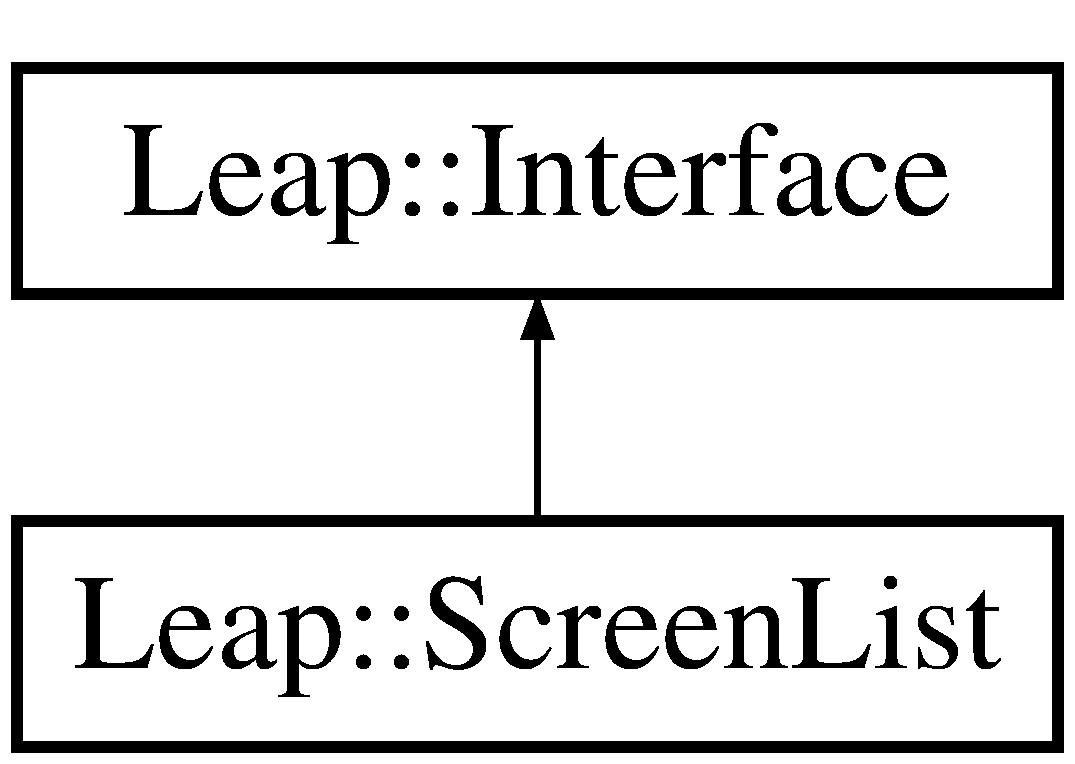
\includegraphics[height=2.000000cm]{class_leap_1_1_screen_list}
\end{center}
\end{figure}
\subsection*{Public Types}
\begin{DoxyCompactItemize}
\item 
typedef \hyperlink{class_leap_1_1_const_list_iterator}{Const\+List\+Iterator}\\*
$<$ \hyperlink{class_leap_1_1_screen_list}{Screen\+List}, \hyperlink{class_leap_1_1_screen}{Screen} $>$ \hyperlink{class_leap_1_1_screen_list_aa5375d780cb454e661f94096dcefd431}{const\+\_\+iterator}
\end{DoxyCompactItemize}
\subsection*{Public Member Functions}
\begin{DoxyCompactItemize}
\item 
\hypertarget{class_leap_1_1_screen_list_a7ce73ebf3b8f5d85f456417a3fd5227c}{{\bfseries Screen\+List} (const \hyperlink{class_leap_1_1_list_base_implementation}{List\+Base\+Implementation}$<$ \hyperlink{class_leap_1_1_screen}{Screen} $>$ \&)}\label{class_leap_1_1_screen_list_a7ce73ebf3b8f5d85f456417a3fd5227c}

\item 
L\+E\+A\+P\+\_\+\+E\+X\+P\+O\+R\+T \hyperlink{class_leap_1_1_screen_list_ac105715f15a022ea47767c548722812d}{Screen\+List} ()
\item 
L\+E\+A\+P\+\_\+\+E\+X\+P\+O\+R\+T int \hyperlink{class_leap_1_1_screen_list_a1c290cc967c6158f15f2ad3fa15a44e9}{count} () const 
\item 
L\+E\+A\+P\+\_\+\+E\+X\+P\+O\+R\+T bool \hyperlink{class_leap_1_1_screen_list_a589cfc780096be2e41b3e9576ac9cd9c}{is\+Empty} () const 
\item 
L\+E\+A\+P\+\_\+\+E\+X\+P\+O\+R\+T \hyperlink{class_leap_1_1_screen}{Screen} \hyperlink{class_leap_1_1_screen_list_aa20953716738fcdb48d457b0a9bfe308}{operator\mbox{[}$\,$\mbox{]}} (int index) const 
\item 
L\+E\+A\+P\+\_\+\+E\+X\+P\+O\+R\+T \hyperlink{class_leap_1_1_screen_list_aa5375d780cb454e661f94096dcefd431}{const\+\_\+iterator} \hyperlink{class_leap_1_1_screen_list_acfff13c200a11512118532f40e187248}{begin} () const 
\item 
L\+E\+A\+P\+\_\+\+E\+X\+P\+O\+R\+T \hyperlink{class_leap_1_1_screen_list_aa5375d780cb454e661f94096dcefd431}{const\+\_\+iterator} \hyperlink{class_leap_1_1_screen_list_a6cebbd92a467aec867535e5ec5f98de1}{end} () const 
\item 
L\+E\+A\+P\+\_\+\+E\+X\+P\+O\+R\+T \hyperlink{class_leap_1_1_screen}{Screen} \hyperlink{class_leap_1_1_screen_list_a3bee50c85325a4935fd6be400a943338}{closest\+Screen\+Hit} (const \hyperlink{class_leap_1_1_pointable}{Pointable} \&pointable) const 
\item 
L\+E\+A\+P\+\_\+\+E\+X\+P\+O\+R\+T \hyperlink{class_leap_1_1_screen}{Screen} \hyperlink{class_leap_1_1_screen_list_aa96701f5c1394f2a386db5e719ca2553}{closest\+Screen\+Hit} (const \hyperlink{struct_leap_1_1_vector}{Vector} \&position, const \hyperlink{struct_leap_1_1_vector}{Vector} \&direction) const 
\item 
L\+E\+A\+P\+\_\+\+E\+X\+P\+O\+R\+T \hyperlink{class_leap_1_1_screen}{Screen} \hyperlink{class_leap_1_1_screen_list_ad5d7a0cc4ddba08e7fcf5d54bfe94255}{closest\+Screen} (const \hyperlink{struct_leap_1_1_vector}{Vector} \&position) const 
\end{DoxyCompactItemize}
\subsection*{Additional Inherited Members}


\subsection{Detailed Description}
The \hyperlink{class_leap_1_1_screen_list}{Screen\+List} class represents a list of \hyperlink{class_leap_1_1_screen}{Screen} objects.

The list always contains at least one entry representing the default screen. If the user has not registered the location of this default screen, then the coordinates, directions, and other values reported by the functions in its \hyperlink{class_leap_1_1_screen}{Screen} object will not be accurate. Other monitor screens only appear in the list if their positions have been registered using the Leap Motion \hyperlink{class_leap_1_1_screen}{Screen} Locator.

Get a \hyperlink{class_leap_1_1_screen_list}{Screen\+List} object by calling \hyperlink{class_leap_1_1_controller_ab6cf5b48ef434b3d58cf8962451f4df3}{Controller\+::located\+Screens()}.


\begin{DoxyCodeInclude}
\end{DoxyCodeInclude}
 \begin{DoxySince}{Since}
1.\+0 
\end{DoxySince}


\subsection{Member Typedef Documentation}
\hypertarget{class_leap_1_1_screen_list_aa5375d780cb454e661f94096dcefd431}{\index{Leap\+::\+Screen\+List@{Leap\+::\+Screen\+List}!const\+\_\+iterator@{const\+\_\+iterator}}
\index{const\+\_\+iterator@{const\+\_\+iterator}!Leap\+::\+Screen\+List@{Leap\+::\+Screen\+List}}
\subsubsection[{const\+\_\+iterator}]{\setlength{\rightskip}{0pt plus 5cm}typedef {\bf Const\+List\+Iterator}$<${\bf Screen\+List}, {\bf Screen}$>$ {\bf Leap\+::\+Screen\+List\+::const\+\_\+iterator}}}\label{class_leap_1_1_screen_list_aa5375d780cb454e661f94096dcefd431}
A C++ iterator type for this \hyperlink{class_leap_1_1_screen_list}{Screen\+List} objects. \begin{DoxySince}{Since}
1.\+0 
\end{DoxySince}


\subsection{Constructor \& Destructor Documentation}
\hypertarget{class_leap_1_1_screen_list_ac105715f15a022ea47767c548722812d}{\index{Leap\+::\+Screen\+List@{Leap\+::\+Screen\+List}!Screen\+List@{Screen\+List}}
\index{Screen\+List@{Screen\+List}!Leap\+::\+Screen\+List@{Leap\+::\+Screen\+List}}
\subsubsection[{Screen\+List}]{\setlength{\rightskip}{0pt plus 5cm}L\+E\+A\+P\+\_\+\+E\+X\+P\+O\+R\+T Leap\+::\+Screen\+List\+::\+Screen\+List (
\begin{DoxyParamCaption}
{}
\end{DoxyParamCaption}
)}}\label{class_leap_1_1_screen_list_ac105715f15a022ea47767c548722812d}
Constructs an empty list of screens. \begin{DoxySince}{Since}
1.\+0 
\end{DoxySince}


\subsection{Member Function Documentation}
\hypertarget{class_leap_1_1_screen_list_acfff13c200a11512118532f40e187248}{\index{Leap\+::\+Screen\+List@{Leap\+::\+Screen\+List}!begin@{begin}}
\index{begin@{begin}!Leap\+::\+Screen\+List@{Leap\+::\+Screen\+List}}
\subsubsection[{begin}]{\setlength{\rightskip}{0pt plus 5cm}L\+E\+A\+P\+\_\+\+E\+X\+P\+O\+R\+T {\bf const\+\_\+iterator} Leap\+::\+Screen\+List\+::begin (
\begin{DoxyParamCaption}
{}
\end{DoxyParamCaption}
) const}}\label{class_leap_1_1_screen_list_acfff13c200a11512118532f40e187248}
The C++ iterator set to the beginning of this \hyperlink{class_leap_1_1_screen_list}{Screen\+List}. \begin{DoxySince}{Since}
1.\+0 
\end{DoxySince}
\hypertarget{class_leap_1_1_screen_list_ad5d7a0cc4ddba08e7fcf5d54bfe94255}{\index{Leap\+::\+Screen\+List@{Leap\+::\+Screen\+List}!closest\+Screen@{closest\+Screen}}
\index{closest\+Screen@{closest\+Screen}!Leap\+::\+Screen\+List@{Leap\+::\+Screen\+List}}
\subsubsection[{closest\+Screen}]{\setlength{\rightskip}{0pt plus 5cm}L\+E\+A\+P\+\_\+\+E\+X\+P\+O\+R\+T {\bf Screen} Leap\+::\+Screen\+List\+::closest\+Screen (
\begin{DoxyParamCaption}
\item[{const {\bf Vector} \&}]{position}
\end{DoxyParamCaption}
) const}}\label{class_leap_1_1_screen_list_ad5d7a0cc4ddba08e7fcf5d54bfe94255}
Gets the \hyperlink{class_leap_1_1_screen}{Screen} closest to the specified position.

The specified position is projected along each screen's normal vector onto the screen's plane. The screen whose projected point is closest to the specified position is returned. Call Screen\+::project(position) on the returned \hyperlink{class_leap_1_1_screen}{Screen} object to find the projected point.


\begin{DoxyCodeInclude}
\end{DoxyCodeInclude}



\begin{DoxyParams}{Parameters}
{\em position} & The position from which to check for screen projection. \\
\hline
\end{DoxyParams}
\begin{DoxyReturn}{Returns}
The closest \hyperlink{class_leap_1_1_screen}{Screen} onto which the specified position is projected. 
\end{DoxyReturn}
\begin{DoxySince}{Since}
1.\+0 
\end{DoxySince}
\hypertarget{class_leap_1_1_screen_list_a3bee50c85325a4935fd6be400a943338}{\index{Leap\+::\+Screen\+List@{Leap\+::\+Screen\+List}!closest\+Screen\+Hit@{closest\+Screen\+Hit}}
\index{closest\+Screen\+Hit@{closest\+Screen\+Hit}!Leap\+::\+Screen\+List@{Leap\+::\+Screen\+List}}
\subsubsection[{closest\+Screen\+Hit}]{\setlength{\rightskip}{0pt plus 5cm}L\+E\+A\+P\+\_\+\+E\+X\+P\+O\+R\+T {\bf Screen} Leap\+::\+Screen\+List\+::closest\+Screen\+Hit (
\begin{DoxyParamCaption}
\item[{const {\bf Pointable} \&}]{pointable}
\end{DoxyParamCaption}
) const}}\label{class_leap_1_1_screen_list_a3bee50c85325a4935fd6be400a943338}
Gets the closest \hyperlink{class_leap_1_1_screen}{Screen} intercepting a ray projecting from the specified \hyperlink{class_leap_1_1_pointable}{Pointable} object.

The projected ray emanates from the \hyperlink{class_leap_1_1_pointable}{Pointable} tip\+Position along the \hyperlink{class_leap_1_1_pointable}{Pointable}'s direction vector. If the projected ray does not intersect any screen surface directly, then the Leap Motion software checks for intersection with the planes extending from the surfaces of the known screens and returns the \hyperlink{class_leap_1_1_screen}{Screen} with the closest intersection.


\begin{DoxyCodeInclude}
\end{DoxyCodeInclude}


If no intersections are found (i.\+e. the ray is directed parallel to or away from all known screens), then an invalid \hyperlink{class_leap_1_1_screen}{Screen} object is returned.

{\itshape Note\+:} Be sure to test whether the \hyperlink{class_leap_1_1_screen}{Screen} object returned by this method is valid. Attempting to use an invalid \hyperlink{class_leap_1_1_screen}{Screen} object will lead to incorrect results.


\begin{DoxyParams}{Parameters}
{\em pointable} & The \hyperlink{class_leap_1_1_pointable}{Pointable} object to check for screen intersection. \\
\hline
\end{DoxyParams}
\begin{DoxyReturn}{Returns}
The closest \hyperlink{class_leap_1_1_screen}{Screen} toward which the specified \hyperlink{class_leap_1_1_pointable}{Pointable} object is pointing, or, if the pointable is not pointing in the direction of any known screen, an invalid \hyperlink{class_leap_1_1_screen}{Screen} object. 
\end{DoxyReturn}
\begin{DoxySince}{Since}
1.\+0 
\end{DoxySince}
\hypertarget{class_leap_1_1_screen_list_aa96701f5c1394f2a386db5e719ca2553}{\index{Leap\+::\+Screen\+List@{Leap\+::\+Screen\+List}!closest\+Screen\+Hit@{closest\+Screen\+Hit}}
\index{closest\+Screen\+Hit@{closest\+Screen\+Hit}!Leap\+::\+Screen\+List@{Leap\+::\+Screen\+List}}
\subsubsection[{closest\+Screen\+Hit}]{\setlength{\rightskip}{0pt plus 5cm}L\+E\+A\+P\+\_\+\+E\+X\+P\+O\+R\+T {\bf Screen} Leap\+::\+Screen\+List\+::closest\+Screen\+Hit (
\begin{DoxyParamCaption}
\item[{const {\bf Vector} \&}]{position, }
\item[{const {\bf Vector} \&}]{direction}
\end{DoxyParamCaption}
) const}}\label{class_leap_1_1_screen_list_aa96701f5c1394f2a386db5e719ca2553}
Gets the closest \hyperlink{class_leap_1_1_screen}{Screen} intercepting a ray projecting from the specified position in the specified direction.

The projected ray emanates from the position along the direction vector. If the projected ray does not intersect any screen surface directly, then the Leap Motion software checks for intersection with the planes extending from the surfaces of the known screens and returns the \hyperlink{class_leap_1_1_screen}{Screen} with the closest intersection.


\begin{DoxyCodeInclude}
\end{DoxyCodeInclude}


If no intersections are found (i.\+e. the ray is directed parallel to or away from all known screens), then an invalid \hyperlink{class_leap_1_1_screen}{Screen} object is returned.

{\itshape Note\+:} Be sure to test whether the \hyperlink{class_leap_1_1_screen}{Screen} object returned by this method is valid. Attempting to use an invalid \hyperlink{class_leap_1_1_screen}{Screen} object will lead to incorrect results.


\begin{DoxyParams}{Parameters}
{\em position} & The position from which to check for screen intersection. \\
\hline
{\em direction} & The direction in which to check for screen intersection. \\
\hline
\end{DoxyParams}
\begin{DoxyReturn}{Returns}
The closest \hyperlink{class_leap_1_1_screen}{Screen} toward which the specified ray is pointing, or, if the ray is not pointing in the direction of any known screen, an invalid \hyperlink{class_leap_1_1_screen}{Screen} object. 
\end{DoxyReturn}
\begin{DoxySince}{Since}
1.\+0 
\end{DoxySince}
\hypertarget{class_leap_1_1_screen_list_a1c290cc967c6158f15f2ad3fa15a44e9}{\index{Leap\+::\+Screen\+List@{Leap\+::\+Screen\+List}!count@{count}}
\index{count@{count}!Leap\+::\+Screen\+List@{Leap\+::\+Screen\+List}}
\subsubsection[{count}]{\setlength{\rightskip}{0pt plus 5cm}L\+E\+A\+P\+\_\+\+E\+X\+P\+O\+R\+T int Leap\+::\+Screen\+List\+::count (
\begin{DoxyParamCaption}
{}
\end{DoxyParamCaption}
) const}}\label{class_leap_1_1_screen_list_a1c290cc967c6158f15f2ad3fa15a44e9}
Returns the number of screens in this list. \begin{DoxyReturn}{Returns}
The number of screens in this list. 
\end{DoxyReturn}
\begin{DoxySince}{Since}
1.\+0 
\end{DoxySince}
\hypertarget{class_leap_1_1_screen_list_a6cebbd92a467aec867535e5ec5f98de1}{\index{Leap\+::\+Screen\+List@{Leap\+::\+Screen\+List}!end@{end}}
\index{end@{end}!Leap\+::\+Screen\+List@{Leap\+::\+Screen\+List}}
\subsubsection[{end}]{\setlength{\rightskip}{0pt plus 5cm}L\+E\+A\+P\+\_\+\+E\+X\+P\+O\+R\+T {\bf const\+\_\+iterator} Leap\+::\+Screen\+List\+::end (
\begin{DoxyParamCaption}
{}
\end{DoxyParamCaption}
) const}}\label{class_leap_1_1_screen_list_a6cebbd92a467aec867535e5ec5f98de1}
The C++ iterator set to the end of this \hyperlink{class_leap_1_1_screen_list}{Screen\+List}. \begin{DoxySince}{Since}
1.\+0 
\end{DoxySince}
\hypertarget{class_leap_1_1_screen_list_a589cfc780096be2e41b3e9576ac9cd9c}{\index{Leap\+::\+Screen\+List@{Leap\+::\+Screen\+List}!is\+Empty@{is\+Empty}}
\index{is\+Empty@{is\+Empty}!Leap\+::\+Screen\+List@{Leap\+::\+Screen\+List}}
\subsubsection[{is\+Empty}]{\setlength{\rightskip}{0pt plus 5cm}L\+E\+A\+P\+\_\+\+E\+X\+P\+O\+R\+T bool Leap\+::\+Screen\+List\+::is\+Empty (
\begin{DoxyParamCaption}
{}
\end{DoxyParamCaption}
) const}}\label{class_leap_1_1_screen_list_a589cfc780096be2e41b3e9576ac9cd9c}
Reports whether the list is empty. \begin{DoxyReturn}{Returns}
True, if the list has no members. 
\end{DoxyReturn}
\begin{DoxySince}{Since}
1.\+0 
\end{DoxySince}
\hypertarget{class_leap_1_1_screen_list_aa20953716738fcdb48d457b0a9bfe308}{\index{Leap\+::\+Screen\+List@{Leap\+::\+Screen\+List}!operator\mbox{[}$\,$\mbox{]}@{operator[]}}
\index{operator\mbox{[}$\,$\mbox{]}@{operator[]}!Leap\+::\+Screen\+List@{Leap\+::\+Screen\+List}}
\subsubsection[{operator[]}]{\setlength{\rightskip}{0pt plus 5cm}L\+E\+A\+P\+\_\+\+E\+X\+P\+O\+R\+T {\bf Screen} Leap\+::\+Screen\+List\+::operator\mbox{[}$\,$\mbox{]} (
\begin{DoxyParamCaption}
\item[{int}]{index}
\end{DoxyParamCaption}
) const}}\label{class_leap_1_1_screen_list_aa20953716738fcdb48d457b0a9bfe308}
Access a list member by its position in the list. 
\begin{DoxyParams}{Parameters}
{\em index} & The zero-\/based list position index. \\
\hline
\end{DoxyParams}
\begin{DoxyReturn}{Returns}
The \hyperlink{class_leap_1_1_screen}{Screen} object at the specified index. 
\end{DoxyReturn}
\begin{DoxySince}{Since}
1.\+0 
\end{DoxySince}


The documentation for this class was generated from the following file\+:\begin{DoxyCompactItemize}
\item 
Interface\+Managers/Leap.\+h\end{DoxyCompactItemize}

\hypertarget{class_leap_1_1_screen_tap_gesture}{\section{Leap\+:\+:Screen\+Tap\+Gesture Class Reference}
\label{class_leap_1_1_screen_tap_gesture}\index{Leap\+::\+Screen\+Tap\+Gesture@{Leap\+::\+Screen\+Tap\+Gesture}}
}


{\ttfamily \#include $<$Leap.\+h$>$}

Inheritance diagram for Leap\+:\+:Screen\+Tap\+Gesture\+:\begin{figure}[H]
\begin{center}
\leavevmode
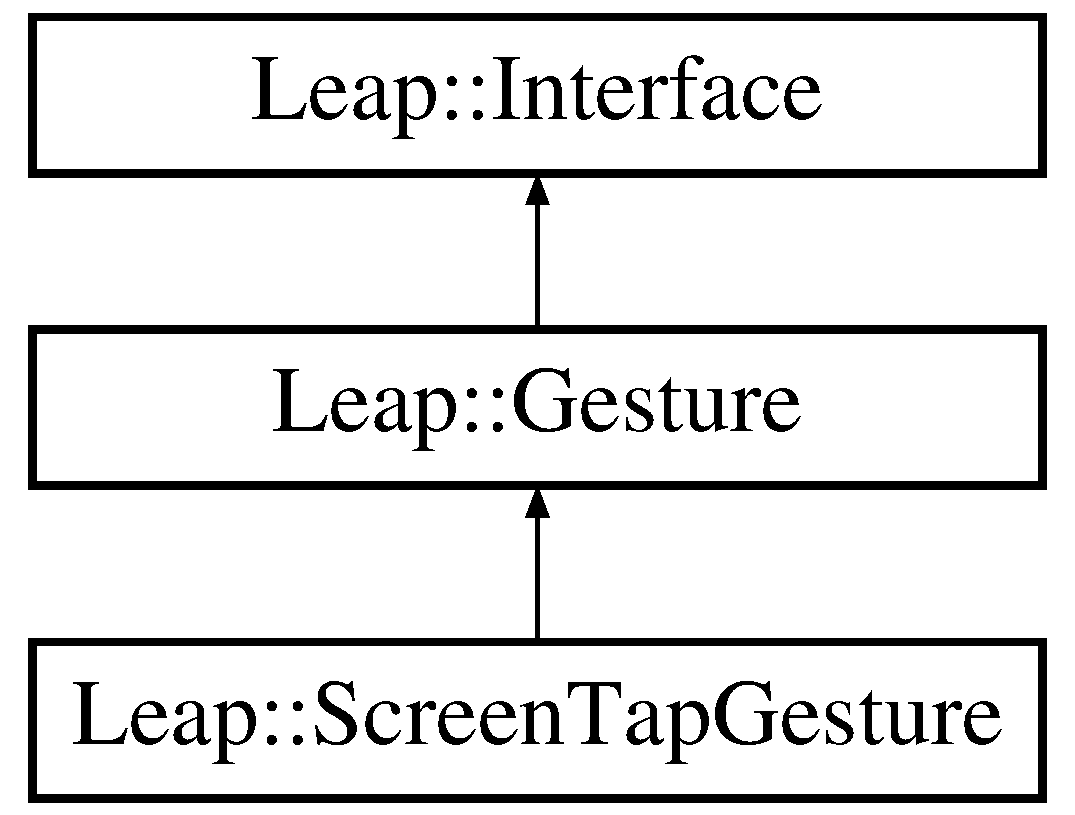
\includegraphics[height=3.000000cm]{class_leap_1_1_screen_tap_gesture}
\end{center}
\end{figure}
\subsection*{Public Member Functions}
\begin{DoxyCompactItemize}
\item 
L\+E\+A\+P\+\_\+\+E\+X\+P\+O\+R\+T \hyperlink{class_leap_1_1_screen_tap_gesture_a9c58b16806da33ae61a090f16eb0f750}{Screen\+Tap\+Gesture} ()
\item 
L\+E\+A\+P\+\_\+\+E\+X\+P\+O\+R\+T \hyperlink{class_leap_1_1_screen_tap_gesture_a1f433e04b2e6adb7a95811c496397ab6}{Screen\+Tap\+Gesture} (const \hyperlink{class_leap_1_1_gesture}{Gesture} \&rhs)
\item 
L\+E\+A\+P\+\_\+\+E\+X\+P\+O\+R\+T \hyperlink{struct_leap_1_1_vector}{Vector} \hyperlink{class_leap_1_1_screen_tap_gesture_aec0c63617e76ed0826cc8276190bc21d}{position} () const 
\item 
L\+E\+A\+P\+\_\+\+E\+X\+P\+O\+R\+T \hyperlink{struct_leap_1_1_vector}{Vector} \hyperlink{class_leap_1_1_screen_tap_gesture_aadee36938c5dc63e26143c116ea130c4}{direction} () const 
\item 
L\+E\+A\+P\+\_\+\+E\+X\+P\+O\+R\+T float \hyperlink{class_leap_1_1_screen_tap_gesture_a08d454596c4b6d944bcdbef61f42249f}{progress} () const 
\item 
L\+E\+A\+P\+\_\+\+E\+X\+P\+O\+R\+T \hyperlink{class_leap_1_1_pointable}{Pointable} \hyperlink{class_leap_1_1_screen_tap_gesture_ab1b2c4ffac3fca7cf5710fa3a84773b4}{pointable} () const 
\end{DoxyCompactItemize}
\subsection*{Static Public Member Functions}
\begin{DoxyCompactItemize}
\item 
static \hyperlink{class_leap_1_1_gesture_a6fa6dd4f28c502f0d55abc6b71c6f9b1}{Type} \hyperlink{class_leap_1_1_screen_tap_gesture_ae967e0ad37fc48faa25044b4a9977f25}{class\+Type} ()
\end{DoxyCompactItemize}
\subsection*{Additional Inherited Members}


\subsection{Detailed Description}
The \hyperlink{class_leap_1_1_screen_tap_gesture}{Screen\+Tap\+Gesture} class represents a tapping gesture by a finger or tool.

A screen tap gesture is recognized when the tip of a finger pokes forward and then springs back to approximately the original postion, as if tapping a vertical screen. The tapping finger must pause briefly before beginning the tap.



{\bfseries Important\+:} To use screen tap gestures in your application, you must enable recognition of the screen tap gesture. You can enable recognition with\+:


\begin{DoxyCodeInclude}
\end{DoxyCodeInclude}


Screen\+Tap gestures are discrete. The \hyperlink{class_leap_1_1_screen_tap_gesture}{Screen\+Tap\+Gesture} object representing a tap always has the state, S\+T\+A\+T\+E\+\_\+\+S\+T\+O\+P. Only one \hyperlink{class_leap_1_1_screen_tap_gesture}{Screen\+Tap\+Gesture} object is created for each screen tap gesture recognized.

You can set the minimum finger movement and velocity required for a movement to be recognized as a screen tap as well as adjust the detection window for evaluating the movement using the config attribute of a connected \hyperlink{class_leap_1_1_controller}{Controller} object. Use the following keys to configure screen tap recognition\+:

\begin{TabularC}{4}
\hline
\rowcolor{lightgray}{\bf Key string }&{\bf Value type }&{\bf Default value }&{\bf Units  }\\\cline{1-4}
Gesture.\+Screen\+Tap.\+Min\+Forward\+Velocity &float &50 &mm/s \\\cline{1-4}
Gesture.\+Screen\+Tap.\+History\+Seconds &float &0.\+1 &s \\\cline{1-4}
Gesture.\+Screen\+Tap.\+Min\+Distance &float &3.\+0 &mm \\\cline{1-4}
\end{TabularC}
The following example demonstrates how to set the screen tap configuration parameters\+:


\begin{DoxyCodeInclude}
\end{DoxyCodeInclude}
 \begin{DoxySince}{Since}
1.\+0 
\end{DoxySince}


\subsection{Constructor \& Destructor Documentation}
\hypertarget{class_leap_1_1_screen_tap_gesture_a9c58b16806da33ae61a090f16eb0f750}{\index{Leap\+::\+Screen\+Tap\+Gesture@{Leap\+::\+Screen\+Tap\+Gesture}!Screen\+Tap\+Gesture@{Screen\+Tap\+Gesture}}
\index{Screen\+Tap\+Gesture@{Screen\+Tap\+Gesture}!Leap\+::\+Screen\+Tap\+Gesture@{Leap\+::\+Screen\+Tap\+Gesture}}
\subsubsection[{Screen\+Tap\+Gesture}]{\setlength{\rightskip}{0pt plus 5cm}L\+E\+A\+P\+\_\+\+E\+X\+P\+O\+R\+T Leap\+::\+Screen\+Tap\+Gesture\+::\+Screen\+Tap\+Gesture (
\begin{DoxyParamCaption}
{}
\end{DoxyParamCaption}
)}}\label{class_leap_1_1_screen_tap_gesture_a9c58b16806da33ae61a090f16eb0f750}
Constructs a new \hyperlink{class_leap_1_1_screen_tap_gesture}{Screen\+Tap\+Gesture} object.

An uninitialized \hyperlink{class_leap_1_1_screen_tap_gesture}{Screen\+Tap\+Gesture} object is considered invalid. Get valid instances of the \hyperlink{class_leap_1_1_screen_tap_gesture}{Screen\+Tap\+Gesture} class from a \hyperlink{class_leap_1_1_frame}{Frame} object. \begin{DoxySince}{Since}
1.\+0 
\end{DoxySince}
\hypertarget{class_leap_1_1_screen_tap_gesture_a1f433e04b2e6adb7a95811c496397ab6}{\index{Leap\+::\+Screen\+Tap\+Gesture@{Leap\+::\+Screen\+Tap\+Gesture}!Screen\+Tap\+Gesture@{Screen\+Tap\+Gesture}}
\index{Screen\+Tap\+Gesture@{Screen\+Tap\+Gesture}!Leap\+::\+Screen\+Tap\+Gesture@{Leap\+::\+Screen\+Tap\+Gesture}}
\subsubsection[{Screen\+Tap\+Gesture}]{\setlength{\rightskip}{0pt plus 5cm}L\+E\+A\+P\+\_\+\+E\+X\+P\+O\+R\+T Leap\+::\+Screen\+Tap\+Gesture\+::\+Screen\+Tap\+Gesture (
\begin{DoxyParamCaption}
\item[{const {\bf Gesture} \&}]{rhs}
\end{DoxyParamCaption}
)}}\label{class_leap_1_1_screen_tap_gesture_a1f433e04b2e6adb7a95811c496397ab6}
Constructs a \hyperlink{class_leap_1_1_screen_tap_gesture}{Screen\+Tap\+Gesture} object from an instance of the \hyperlink{class_leap_1_1_gesture}{Gesture} class.


\begin{DoxyParams}{Parameters}
{\em rhs} & The \hyperlink{class_leap_1_1_gesture}{Gesture} instance to specialize. This \hyperlink{class_leap_1_1_gesture}{Gesture} instance must be a \hyperlink{class_leap_1_1_screen_tap_gesture}{Screen\+Tap\+Gesture} object. \\
\hline
\end{DoxyParams}
\begin{DoxySince}{Since}
1.\+0 
\end{DoxySince}


\subsection{Member Function Documentation}
\hypertarget{class_leap_1_1_screen_tap_gesture_ae967e0ad37fc48faa25044b4a9977f25}{\index{Leap\+::\+Screen\+Tap\+Gesture@{Leap\+::\+Screen\+Tap\+Gesture}!class\+Type@{class\+Type}}
\index{class\+Type@{class\+Type}!Leap\+::\+Screen\+Tap\+Gesture@{Leap\+::\+Screen\+Tap\+Gesture}}
\subsubsection[{class\+Type}]{\setlength{\rightskip}{0pt plus 5cm}static {\bf Type} Leap\+::\+Screen\+Tap\+Gesture\+::class\+Type (
\begin{DoxyParamCaption}
{}
\end{DoxyParamCaption}
)\hspace{0.3cm}{\ttfamily [inline]}, {\ttfamily [static]}}}\label{class_leap_1_1_screen_tap_gesture_ae967e0ad37fc48faa25044b4a9977f25}
The screen tap gesture type.

\begin{DoxyReturn}{Returns}
Type The type value designating a screen tap gesture. 
\end{DoxyReturn}
\begin{DoxySince}{Since}
1.\+0 
\end{DoxySince}
\hypertarget{class_leap_1_1_screen_tap_gesture_aadee36938c5dc63e26143c116ea130c4}{\index{Leap\+::\+Screen\+Tap\+Gesture@{Leap\+::\+Screen\+Tap\+Gesture}!direction@{direction}}
\index{direction@{direction}!Leap\+::\+Screen\+Tap\+Gesture@{Leap\+::\+Screen\+Tap\+Gesture}}
\subsubsection[{direction}]{\setlength{\rightskip}{0pt plus 5cm}L\+E\+A\+P\+\_\+\+E\+X\+P\+O\+R\+T {\bf Vector} Leap\+::\+Screen\+Tap\+Gesture\+::direction (
\begin{DoxyParamCaption}
{}
\end{DoxyParamCaption}
) const}}\label{class_leap_1_1_screen_tap_gesture_aadee36938c5dc63e26143c116ea130c4}
The direction of finger tip motion.

\begin{DoxyReturn}{Returns}
\hyperlink{struct_leap_1_1_vector}{Vector} A unit direction vector. 
\end{DoxyReturn}
\begin{DoxySince}{Since}
1.\+0 
\end{DoxySince}
\hypertarget{class_leap_1_1_screen_tap_gesture_ab1b2c4ffac3fca7cf5710fa3a84773b4}{\index{Leap\+::\+Screen\+Tap\+Gesture@{Leap\+::\+Screen\+Tap\+Gesture}!pointable@{pointable}}
\index{pointable@{pointable}!Leap\+::\+Screen\+Tap\+Gesture@{Leap\+::\+Screen\+Tap\+Gesture}}
\subsubsection[{pointable}]{\setlength{\rightskip}{0pt plus 5cm}L\+E\+A\+P\+\_\+\+E\+X\+P\+O\+R\+T {\bf Pointable} Leap\+::\+Screen\+Tap\+Gesture\+::pointable (
\begin{DoxyParamCaption}
{}
\end{DoxyParamCaption}
) const}}\label{class_leap_1_1_screen_tap_gesture_ab1b2c4ffac3fca7cf5710fa3a84773b4}
The finger performing the screen tap gesture.

\begin{DoxyReturn}{Returns}
\hyperlink{class_leap_1_1_pointable}{Pointable} A \hyperlink{class_leap_1_1_pointable}{Pointable} object representing the tapping finger. 
\end{DoxyReturn}
\begin{DoxySince}{Since}
1.\+0 
\end{DoxySince}
\hypertarget{class_leap_1_1_screen_tap_gesture_aec0c63617e76ed0826cc8276190bc21d}{\index{Leap\+::\+Screen\+Tap\+Gesture@{Leap\+::\+Screen\+Tap\+Gesture}!position@{position}}
\index{position@{position}!Leap\+::\+Screen\+Tap\+Gesture@{Leap\+::\+Screen\+Tap\+Gesture}}
\subsubsection[{position}]{\setlength{\rightskip}{0pt plus 5cm}L\+E\+A\+P\+\_\+\+E\+X\+P\+O\+R\+T {\bf Vector} Leap\+::\+Screen\+Tap\+Gesture\+::position (
\begin{DoxyParamCaption}
{}
\end{DoxyParamCaption}
) const}}\label{class_leap_1_1_screen_tap_gesture_aec0c63617e76ed0826cc8276190bc21d}
The position where the screen tap is registered.

\begin{DoxyReturn}{Returns}
\hyperlink{struct_leap_1_1_vector}{Vector} A \hyperlink{struct_leap_1_1_vector}{Vector} containing the coordinates of screen tap location. 
\end{DoxyReturn}
\begin{DoxySince}{Since}
1.\+0 
\end{DoxySince}
\hypertarget{class_leap_1_1_screen_tap_gesture_a08d454596c4b6d944bcdbef61f42249f}{\index{Leap\+::\+Screen\+Tap\+Gesture@{Leap\+::\+Screen\+Tap\+Gesture}!progress@{progress}}
\index{progress@{progress}!Leap\+::\+Screen\+Tap\+Gesture@{Leap\+::\+Screen\+Tap\+Gesture}}
\subsubsection[{progress}]{\setlength{\rightskip}{0pt plus 5cm}L\+E\+A\+P\+\_\+\+E\+X\+P\+O\+R\+T float Leap\+::\+Screen\+Tap\+Gesture\+::progress (
\begin{DoxyParamCaption}
{}
\end{DoxyParamCaption}
) const}}\label{class_leap_1_1_screen_tap_gesture_a08d454596c4b6d944bcdbef61f42249f}
The progess value is always 1.\+0 for a screen tap gesture.

\begin{DoxyReturn}{Returns}
float The value 1.\+0. 
\end{DoxyReturn}
\begin{DoxySince}{Since}
1.\+0 
\end{DoxySince}


The documentation for this class was generated from the following file\+:\begin{DoxyCompactItemize}
\item 
Interface\+Managers/Leap.\+h\end{DoxyCompactItemize}

\hypertarget{class_simon_controller}{\section{Simon\+Controller Class Reference}
\label{class_simon_controller}\index{Simon\+Controller@{Simon\+Controller}}
}


{\ttfamily \#include $<$simoncontroller.\+h$>$}

Inheritance diagram for Simon\+Controller\+:\begin{figure}[H]
\begin{center}
\leavevmode
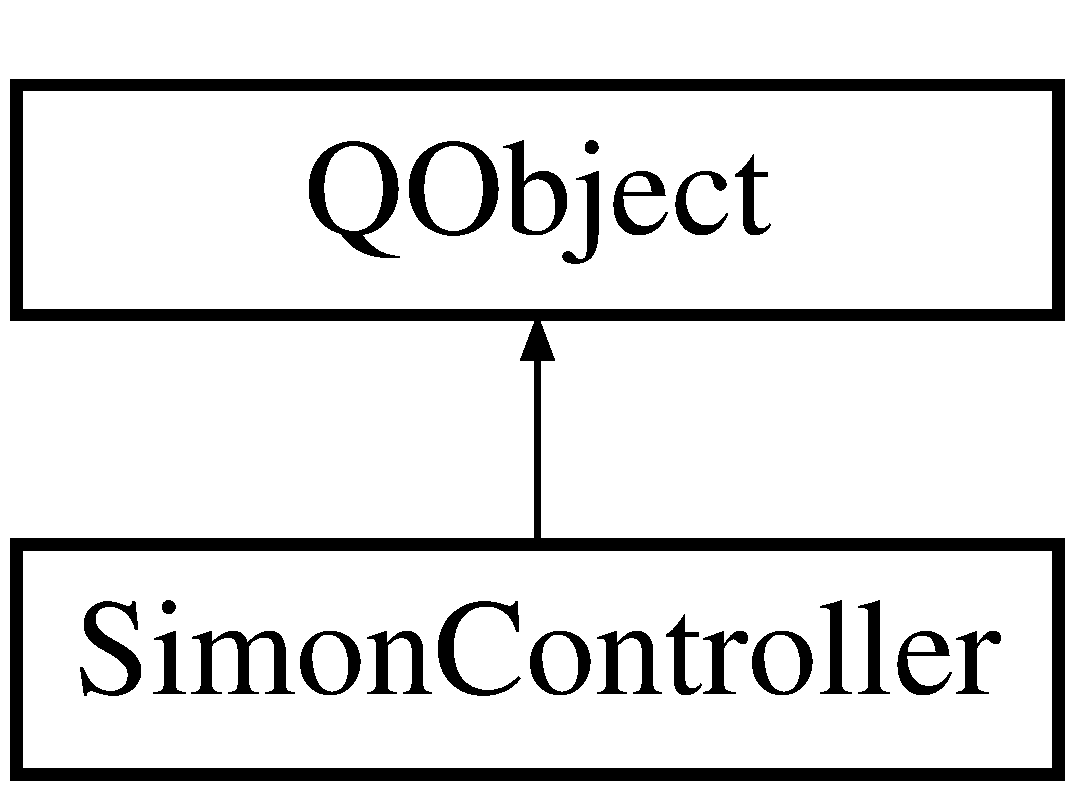
\includegraphics[height=2.000000cm]{class_simon_controller}
\end{center}
\end{figure}
\subsection*{Public Slots}
\begin{DoxyCompactItemize}
\item 
void \hyperlink{class_simon_controller_a192ee3ae7fa66e2c7ca71c504884dc26}{next\+Game} ()
\end{DoxyCompactItemize}
\subsection*{Public Member Functions}
\begin{DoxyCompactItemize}
\item 
\hyperlink{class_simon_controller_a16bdca59b946631ef5542dd351b8ca1a}{Simon\+Controller} ()
\item 
\hyperlink{class_simon_controller_a7690ecb37c9c83a6c0b0bc6000f9c16e}{$\sim$\+Simon\+Controller} ()
\item 
void \hyperlink{class_simon_controller_ac3d7312cfdfceb9bde664bd691b5d871}{start} ()
\end{DoxyCompactItemize}


\subsection{Detailed Description}
A state machine class that manages simon games. This guy does little more than calling the individual games. Each game handles its own setup and destruction. 

\subsection{Constructor \& Destructor Documentation}
\hypertarget{class_simon_controller_a16bdca59b946631ef5542dd351b8ca1a}{\index{Simon\+Controller@{Simon\+Controller}!Simon\+Controller@{Simon\+Controller}}
\index{Simon\+Controller@{Simon\+Controller}!Simon\+Controller@{Simon\+Controller}}
\subsubsection[{Simon\+Controller}]{\setlength{\rightskip}{0pt plus 5cm}Simon\+Controller\+::\+Simon\+Controller (
\begin{DoxyParamCaption}
{}
\end{DoxyParamCaption}
)}}\label{class_simon_controller_a16bdca59b946631ef5542dd351b8ca1a}
Constructor \hypertarget{class_simon_controller_a7690ecb37c9c83a6c0b0bc6000f9c16e}{\index{Simon\+Controller@{Simon\+Controller}!````~Simon\+Controller@{$\sim$\+Simon\+Controller}}
\index{````~Simon\+Controller@{$\sim$\+Simon\+Controller}!Simon\+Controller@{Simon\+Controller}}
\subsubsection[{$\sim$\+Simon\+Controller}]{\setlength{\rightskip}{0pt plus 5cm}Simon\+Controller\+::$\sim$\+Simon\+Controller (
\begin{DoxyParamCaption}
{}
\end{DoxyParamCaption}
)}}\label{class_simon_controller_a7690ecb37c9c83a6c0b0bc6000f9c16e}
Destructor 

\subsection{Member Function Documentation}
\hypertarget{class_simon_controller_a192ee3ae7fa66e2c7ca71c504884dc26}{\index{Simon\+Controller@{Simon\+Controller}!next\+Game@{next\+Game}}
\index{next\+Game@{next\+Game}!Simon\+Controller@{Simon\+Controller}}
\subsubsection[{next\+Game}]{\setlength{\rightskip}{0pt plus 5cm}void Simon\+Controller\+::next\+Game (
\begin{DoxyParamCaption}
{}
\end{DoxyParamCaption}
)\hspace{0.3cm}{\ttfamily [slot]}}}\label{class_simon_controller_a192ee3ae7fa66e2c7ca71c504884dc26}
Goes to the next game \hypertarget{class_simon_controller_ac3d7312cfdfceb9bde664bd691b5d871}{\index{Simon\+Controller@{Simon\+Controller}!start@{start}}
\index{start@{start}!Simon\+Controller@{Simon\+Controller}}
\subsubsection[{start}]{\setlength{\rightskip}{0pt plus 5cm}void Simon\+Controller\+::start (
\begin{DoxyParamCaption}
{}
\end{DoxyParamCaption}
)}}\label{class_simon_controller_ac3d7312cfdfceb9bde664bd691b5d871}
Starts running through the games listed in \hyperlink{class_trial_data}{Trial\+Data} 

The documentation for this class was generated from the following files\+:\begin{DoxyCompactItemize}
\item 
State\+Machines/simoncontroller.\+h\item 
State\+Machines/simoncontroller.\+cpp\end{DoxyCompactItemize}

\hypertarget{class_simon_game}{\section{Simon\+Game Class Reference}
\label{class_simon_game}\index{Simon\+Game@{Simon\+Game}}
}


{\ttfamily \#include $<$simongame.\+h$>$}

Inheritance diagram for Simon\+Game\+:\begin{figure}[H]
\begin{center}
\leavevmode
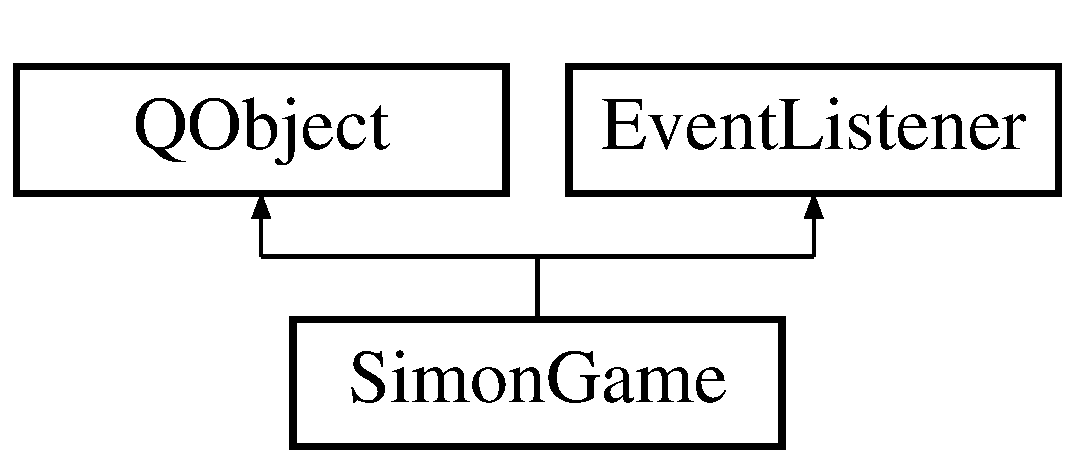
\includegraphics[height=2.000000cm]{class_simon_game}
\end{center}
\end{figure}
\subsection*{Public Slots}
\begin{DoxyCompactItemize}
\item 
void \hyperlink{class_simon_game_a675881171d32be130c1eaba36b7c56d8}{on\+Timeout} ()
\end{DoxyCompactItemize}
\subsection*{Signals}
\begin{DoxyCompactItemize}
\item 
void \hyperlink{class_simon_game_a6d13e176d256c18c5e00d8cac979b239}{game\+Over} ()
\end{DoxyCompactItemize}
\subsection*{Public Member Functions}
\begin{DoxyCompactItemize}
\item 
\hyperlink{class_simon_game_abb9ef25e4158c51128d4b5b9214d0547}{Simon\+Game} (\hyperlink{class_game_data}{Game\+Data} $\ast$game\+Data)
\item 
\hyperlink{class_simon_game_a36ec045acaa79798534b781c554a8df8}{$\sim$\+Simon\+Game} ()
\item 
void \hyperlink{class_simon_game_a3195d192b13c7ee5eba290e4d265427a}{start} ()
\item 
void \hyperlink{class_simon_game_a35dc2ba138666e626ef663ef6b954f4b}{on\+Event} (Quadrant\+I\+D q, Event\+Type e)
\end{DoxyCompactItemize}


\subsection{Detailed Description}
A state machine class that manages the run loop for a single game. 

\subsection{Constructor \& Destructor Documentation}
\hypertarget{class_simon_game_abb9ef25e4158c51128d4b5b9214d0547}{\index{Simon\+Game@{Simon\+Game}!Simon\+Game@{Simon\+Game}}
\index{Simon\+Game@{Simon\+Game}!Simon\+Game@{Simon\+Game}}
\subsubsection[{Simon\+Game}]{\setlength{\rightskip}{0pt plus 5cm}Simon\+Game\+::\+Simon\+Game (
\begin{DoxyParamCaption}
\item[{{\bf Game\+Data} $\ast$}]{game\+Data}
\end{DoxyParamCaption}
)}}\label{class_simon_game_abb9ef25e4158c51128d4b5b9214d0547}
Constructor -\/ takes a \hyperlink{class_game_data}{Game\+Data} instance representing the current game configuration \hypertarget{class_simon_game_a36ec045acaa79798534b781c554a8df8}{\index{Simon\+Game@{Simon\+Game}!````~Simon\+Game@{$\sim$\+Simon\+Game}}
\index{````~Simon\+Game@{$\sim$\+Simon\+Game}!Simon\+Game@{Simon\+Game}}
\subsubsection[{$\sim$\+Simon\+Game}]{\setlength{\rightskip}{0pt plus 5cm}Simon\+Game\+::$\sim$\+Simon\+Game (
\begin{DoxyParamCaption}
{}
\end{DoxyParamCaption}
)}}\label{class_simon_game_a36ec045acaa79798534b781c554a8df8}
Destructor -\/ removes eventlisteners, cleanup 

\subsection{Member Function Documentation}
\hypertarget{class_simon_game_a6d13e176d256c18c5e00d8cac979b239}{\index{Simon\+Game@{Simon\+Game}!game\+Over@{game\+Over}}
\index{game\+Over@{game\+Over}!Simon\+Game@{Simon\+Game}}
\subsubsection[{game\+Over}]{\setlength{\rightskip}{0pt plus 5cm}void Simon\+Game\+::game\+Over (
\begin{DoxyParamCaption}
{}
\end{DoxyParamCaption}
)\hspace{0.3cm}{\ttfamily [signal]}}}\label{class_simon_game_a6d13e176d256c18c5e00d8cac979b239}
Signal the end of this game \hypertarget{class_simon_game_a35dc2ba138666e626ef663ef6b954f4b}{\index{Simon\+Game@{Simon\+Game}!on\+Event@{on\+Event}}
\index{on\+Event@{on\+Event}!Simon\+Game@{Simon\+Game}}
\subsubsection[{on\+Event}]{\setlength{\rightskip}{0pt plus 5cm}void Simon\+Game\+::on\+Event (
\begin{DoxyParamCaption}
\item[{Quadrant\+I\+D}]{q, }
\item[{Event\+Type}]{e}
\end{DoxyParamCaption}
)}}\label{class_simon_game_a35dc2ba138666e626ef663ef6b954f4b}
Respond to an Event\+Listener event \hypertarget{class_simon_game_a675881171d32be130c1eaba36b7c56d8}{\index{Simon\+Game@{Simon\+Game}!on\+Timeout@{on\+Timeout}}
\index{on\+Timeout@{on\+Timeout}!Simon\+Game@{Simon\+Game}}
\subsubsection[{on\+Timeout}]{\setlength{\rightskip}{0pt plus 5cm}void Simon\+Game\+::on\+Timeout (
\begin{DoxyParamCaption}
{}
\end{DoxyParamCaption}
)\hspace{0.3cm}{\ttfamily [slot]}}}\label{class_simon_game_a675881171d32be130c1eaba36b7c56d8}
Called when time is up \hypertarget{class_simon_game_a3195d192b13c7ee5eba290e4d265427a}{\index{Simon\+Game@{Simon\+Game}!start@{start}}
\index{start@{start}!Simon\+Game@{Simon\+Game}}
\subsubsection[{start}]{\setlength{\rightskip}{0pt plus 5cm}void Simon\+Game\+::start (
\begin{DoxyParamCaption}
{}
\end{DoxyParamCaption}
)}}\label{class_simon_game_a3195d192b13c7ee5eba290e4d265427a}
Start the loop 

The documentation for this class was generated from the following files\+:\begin{DoxyCompactItemize}
\item 
State\+Machines/simongame.\+h\item 
State\+Machines/simongame.\+cpp\end{DoxyCompactItemize}

\hypertarget{class_simon_u_i}{\section{Simon\+U\+I Class Reference}
\label{class_simon_u_i}\index{Simon\+U\+I@{Simon\+U\+I}}
}


{\ttfamily \#include $<$simonui.\+h$>$}

Inheritance diagram for Simon\+U\+I\+:\begin{figure}[H]
\begin{center}
\leavevmode
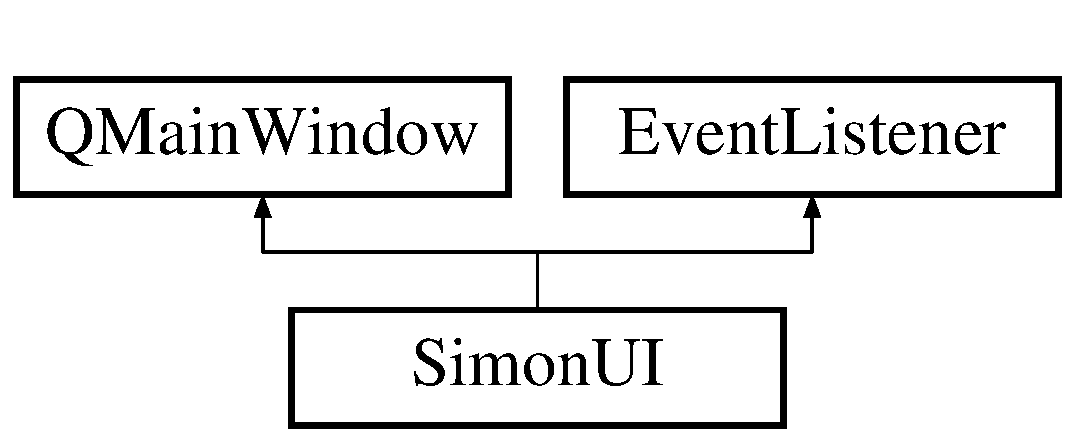
\includegraphics[height=2.000000cm]{class_simon_u_i}
\end{center}
\end{figure}
\subsection*{Public Member Functions}
\begin{DoxyCompactItemize}
\item 
\hyperlink{class_simon_u_i_aa39db09f5a4cdeb3083de44da983690e}{Simon\+U\+I} (Q\+Widget $\ast$parent=0)
\item 
\hyperlink{class_simon_u_i_a1158d78365109c8bb21563df5bcc7239}{$\sim$\+Simon\+U\+I} ()
\item 
void \hyperlink{class_simon_u_i_a9a8de04376322efe03495a873d8e08d9}{on\+Event} (Quadrant\+I\+D q, Event\+Type e)
\item 
void \hyperlink{class_simon_u_i_ad5e1e4ea6e411396afb181e29b3f2a25}{set\+Variables} (Color\+Type color, Sound\+Type sound)
\item 
void \hyperlink{class_simon_u_i_afc9c076401c1407d5a82751fadfd77ce}{enable\+Menu} (bool enable)
\item 
void \hyperlink{class_simon_u_i_a408401c0f50f6c65c14af8742b74e571}{press\+Quadrant} (Quadrant\+I\+D q)
\item 
void \hyperlink{class_simon_u_i_ab3e596178a1ef6f35313b9f67df8d301}{hover\+Quadrant} (Quadrant\+I\+D q)
\end{DoxyCompactItemize}
\subsection*{Static Public Member Functions}
\begin{DoxyCompactItemize}
\item 
static \hyperlink{class_simon_u_i}{Simon\+U\+I} $\ast$ \hyperlink{class_simon_u_i_af2a6bcb286d56a2ef463c46884f58b8c}{get\+Main\+Window} ()
\end{DoxyCompactItemize}


\subsection{Detailed Description}
The main window of the game. Displays the simon board. 

\subsection{Constructor \& Destructor Documentation}
\hypertarget{class_simon_u_i_aa39db09f5a4cdeb3083de44da983690e}{\index{Simon\+U\+I@{Simon\+U\+I}!Simon\+U\+I@{Simon\+U\+I}}
\index{Simon\+U\+I@{Simon\+U\+I}!Simon\+U\+I@{Simon\+U\+I}}
\subsubsection[{Simon\+U\+I}]{\setlength{\rightskip}{0pt plus 5cm}Simon\+U\+I\+::\+Simon\+U\+I (
\begin{DoxyParamCaption}
\item[{Q\+Widget $\ast$}]{parent = {\ttfamily 0}}
\end{DoxyParamCaption}
)\hspace{0.3cm}{\ttfamily [explicit]}}}\label{class_simon_u_i_aa39db09f5a4cdeb3083de44da983690e}
Constructor \hypertarget{class_simon_u_i_a1158d78365109c8bb21563df5bcc7239}{\index{Simon\+U\+I@{Simon\+U\+I}!````~Simon\+U\+I@{$\sim$\+Simon\+U\+I}}
\index{````~Simon\+U\+I@{$\sim$\+Simon\+U\+I}!Simon\+U\+I@{Simon\+U\+I}}
\subsubsection[{$\sim$\+Simon\+U\+I}]{\setlength{\rightskip}{0pt plus 5cm}Simon\+U\+I\+::$\sim$\+Simon\+U\+I (
\begin{DoxyParamCaption}
{}
\end{DoxyParamCaption}
)}}\label{class_simon_u_i_a1158d78365109c8bb21563df5bcc7239}
Destructor 

\subsection{Member Function Documentation}
\hypertarget{class_simon_u_i_afc9c076401c1407d5a82751fadfd77ce}{\index{Simon\+U\+I@{Simon\+U\+I}!enable\+Menu@{enable\+Menu}}
\index{enable\+Menu@{enable\+Menu}!Simon\+U\+I@{Simon\+U\+I}}
\subsubsection[{enable\+Menu}]{\setlength{\rightskip}{0pt plus 5cm}void Simon\+U\+I\+::enable\+Menu (
\begin{DoxyParamCaption}
\item[{bool}]{enable}
\end{DoxyParamCaption}
)}}\label{class_simon_u_i_afc9c076401c1407d5a82751fadfd77ce}
Used to disable menu during gameplay \hypertarget{class_simon_u_i_af2a6bcb286d56a2ef463c46884f58b8c}{\index{Simon\+U\+I@{Simon\+U\+I}!get\+Main\+Window@{get\+Main\+Window}}
\index{get\+Main\+Window@{get\+Main\+Window}!Simon\+U\+I@{Simon\+U\+I}}
\subsubsection[{get\+Main\+Window}]{\setlength{\rightskip}{0pt plus 5cm}{\bf Simon\+U\+I} $\ast$ Simon\+U\+I\+::get\+Main\+Window (
\begin{DoxyParamCaption}
{}
\end{DoxyParamCaption}
)\hspace{0.3cm}{\ttfamily [static]}}}\label{class_simon_u_i_af2a6bcb286d56a2ef463c46884f58b8c}
Static method, returns the singleton instance \hypertarget{class_simon_u_i_ab3e596178a1ef6f35313b9f67df8d301}{\index{Simon\+U\+I@{Simon\+U\+I}!hover\+Quadrant@{hover\+Quadrant}}
\index{hover\+Quadrant@{hover\+Quadrant}!Simon\+U\+I@{Simon\+U\+I}}
\subsubsection[{hover\+Quadrant}]{\setlength{\rightskip}{0pt plus 5cm}void Simon\+U\+I\+::hover\+Quadrant (
\begin{DoxyParamCaption}
\item[{Quadrant\+I\+D}]{q}
\end{DoxyParamCaption}
)}}\label{class_simon_u_i_ab3e596178a1ef6f35313b9f67df8d301}
For playback -\/ hover \hypertarget{class_simon_u_i_a9a8de04376322efe03495a873d8e08d9}{\index{Simon\+U\+I@{Simon\+U\+I}!on\+Event@{on\+Event}}
\index{on\+Event@{on\+Event}!Simon\+U\+I@{Simon\+U\+I}}
\subsubsection[{on\+Event}]{\setlength{\rightskip}{0pt plus 5cm}void Simon\+U\+I\+::on\+Event (
\begin{DoxyParamCaption}
\item[{Quadrant\+I\+D}]{q, }
\item[{Event\+Type}]{e}
\end{DoxyParamCaption}
)\hspace{0.3cm}{\ttfamily [virtual]}}}\label{class_simon_u_i_a9a8de04376322efe03495a873d8e08d9}
Implements \hyperlink{class_event_listener}{Event\+Listener}. Called on input events 

Reimplemented from \hyperlink{class_event_listener_a19232875c793366beb4d8edb0cc89164}{Event\+Listener}.

\hypertarget{class_simon_u_i_a408401c0f50f6c65c14af8742b74e571}{\index{Simon\+U\+I@{Simon\+U\+I}!press\+Quadrant@{press\+Quadrant}}
\index{press\+Quadrant@{press\+Quadrant}!Simon\+U\+I@{Simon\+U\+I}}
\subsubsection[{press\+Quadrant}]{\setlength{\rightskip}{0pt plus 5cm}void Simon\+U\+I\+::press\+Quadrant (
\begin{DoxyParamCaption}
\item[{Quadrant\+I\+D}]{q}
\end{DoxyParamCaption}
)}}\label{class_simon_u_i_a408401c0f50f6c65c14af8742b74e571}
For playback -\/ press \hypertarget{class_simon_u_i_ad5e1e4ea6e411396afb181e29b3f2a25}{\index{Simon\+U\+I@{Simon\+U\+I}!set\+Variables@{set\+Variables}}
\index{set\+Variables@{set\+Variables}!Simon\+U\+I@{Simon\+U\+I}}
\subsubsection[{set\+Variables}]{\setlength{\rightskip}{0pt plus 5cm}void Simon\+U\+I\+::set\+Variables (
\begin{DoxyParamCaption}
\item[{Color\+Type}]{color, }
\item[{Sound\+Type}]{sound}
\end{DoxyParamCaption}
)}}\label{class_simon_u_i_ad5e1e4ea6e411396afb181e29b3f2a25}
Discard current quadrants, create new ones 

The documentation for this class was generated from the following files\+:\begin{DoxyCompactItemize}
\item 
U\+I/simonui.\+h\item 
U\+I/simonui.\+cpp\end{DoxyCompactItemize}

\hypertarget{class_leap_1_1_swipe_gesture}{\section{Leap\+:\+:Swipe\+Gesture Class Reference}
\label{class_leap_1_1_swipe_gesture}\index{Leap\+::\+Swipe\+Gesture@{Leap\+::\+Swipe\+Gesture}}
}


{\ttfamily \#include $<$Leap.\+h$>$}

Inheritance diagram for Leap\+:\+:Swipe\+Gesture\+:\begin{figure}[H]
\begin{center}
\leavevmode
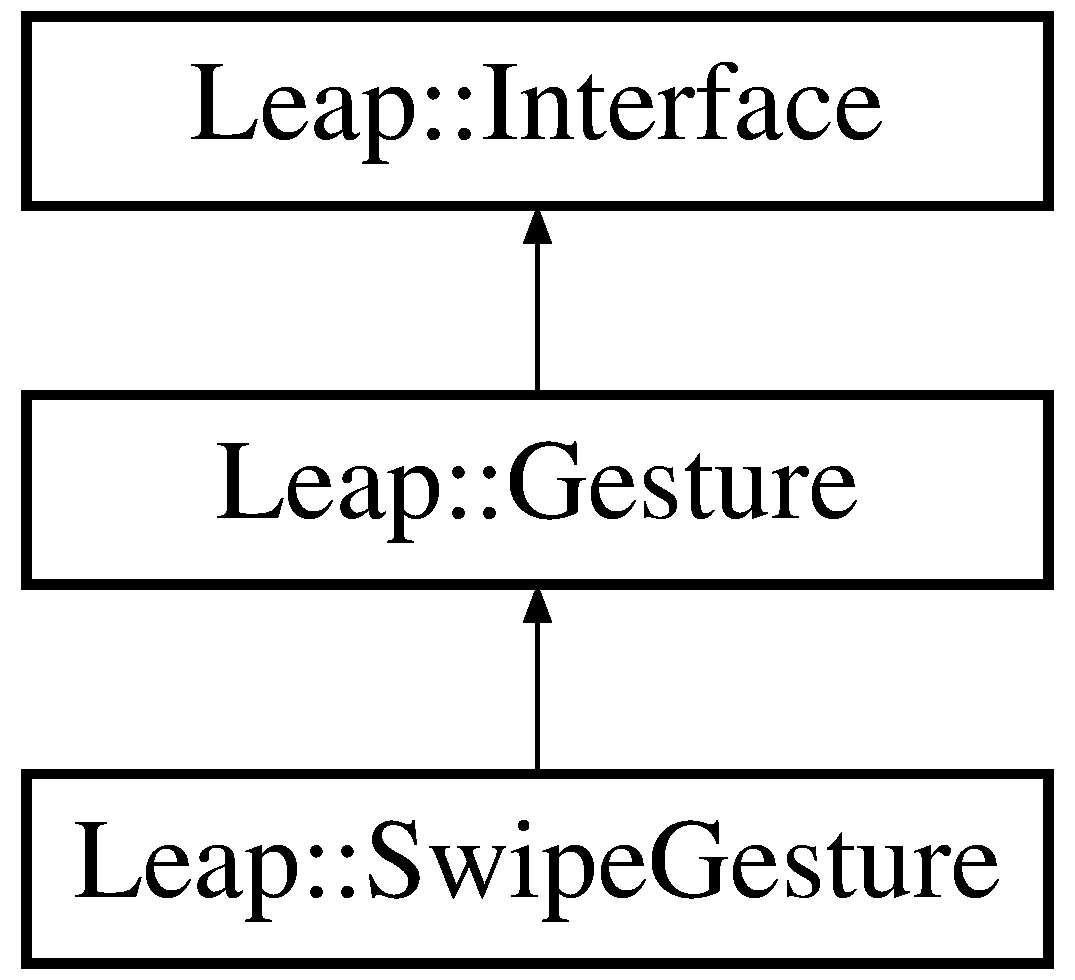
\includegraphics[height=3.000000cm]{class_leap_1_1_swipe_gesture}
\end{center}
\end{figure}
\subsection*{Public Member Functions}
\begin{DoxyCompactItemize}
\item 
L\+E\+A\+P\+\_\+\+E\+X\+P\+O\+R\+T \hyperlink{class_leap_1_1_swipe_gesture_ac4698d7bf0a8ef15a92b00866a31fb7f}{Swipe\+Gesture} (const \hyperlink{class_leap_1_1_gesture}{Gesture} \&rhs)
\item 
L\+E\+A\+P\+\_\+\+E\+X\+P\+O\+R\+T \hyperlink{struct_leap_1_1_vector}{Vector} \hyperlink{class_leap_1_1_swipe_gesture_a273bcdcb7e67cdb1c35fc0a80c7dfabc}{start\+Position} () const 
\item 
L\+E\+A\+P\+\_\+\+E\+X\+P\+O\+R\+T \hyperlink{struct_leap_1_1_vector}{Vector} \hyperlink{class_leap_1_1_swipe_gesture_a14e074dad90fc86eec1144edce20c4bb}{position} () const 
\item 
L\+E\+A\+P\+\_\+\+E\+X\+P\+O\+R\+T \hyperlink{struct_leap_1_1_vector}{Vector} \hyperlink{class_leap_1_1_swipe_gesture_ab9fe4410a8bb19a993a514115a8fb161}{direction} () const 
\item 
L\+E\+A\+P\+\_\+\+E\+X\+P\+O\+R\+T float \hyperlink{class_leap_1_1_swipe_gesture_a8da056c9faa0a941f43d34f3a489ecc7}{speed} () const 
\item 
L\+E\+A\+P\+\_\+\+E\+X\+P\+O\+R\+T \hyperlink{class_leap_1_1_pointable}{Pointable} \hyperlink{class_leap_1_1_swipe_gesture_a51712b0e742448e3f51549e5300aceee}{pointable} () const 
\end{DoxyCompactItemize}
\subsection*{Static Public Member Functions}
\begin{DoxyCompactItemize}
\item 
static \hyperlink{class_leap_1_1_gesture_a6fa6dd4f28c502f0d55abc6b71c6f9b1}{Type} \hyperlink{class_leap_1_1_swipe_gesture_a0dac022eaf599cf5393af9456cb9896e}{class\+Type} ()
\end{DoxyCompactItemize}
\subsection*{Additional Inherited Members}


\subsection{Detailed Description}
The \hyperlink{class_leap_1_1_swipe_gesture}{Swipe\+Gesture} class represents a swiping motion of a finger or tool.



{\bfseries Important\+:} To use swipe gestures in your application, you must enable recognition of the swipe gesture. You can enable recognition with\+:


\begin{DoxyCodeInclude}
\end{DoxyCodeInclude}


Swipe gestures are continuous.

You can set the minimum length and velocity required for a movement to be recognized as a swipe using the config attribute of a connected \hyperlink{class_leap_1_1_controller}{Controller} object. Use the following keys to configure swipe recognition\+:

\begin{TabularC}{4}
\hline
\rowcolor{lightgray}{\bf Key string }&{\bf Value type }&{\bf Default value }&{\bf Units  }\\\cline{1-4}
Gesture.\+Swipe.\+Min\+Length &float &150 &mm \\\cline{1-4}
Gesture.\+Swipe.\+Min\+Velocity &float &1000 &mm/s \\\cline{1-4}
\end{TabularC}
The following example demonstrates how to set the swipe configuration parameters\+:


\begin{DoxyCodeInclude}
\end{DoxyCodeInclude}
 \begin{DoxySince}{Since}
1.\+0 
\end{DoxySince}


\subsection{Constructor \& Destructor Documentation}
\hypertarget{class_leap_1_1_swipe_gesture_ac4698d7bf0a8ef15a92b00866a31fb7f}{\index{Leap\+::\+Swipe\+Gesture@{Leap\+::\+Swipe\+Gesture}!Swipe\+Gesture@{Swipe\+Gesture}}
\index{Swipe\+Gesture@{Swipe\+Gesture}!Leap\+::\+Swipe\+Gesture@{Leap\+::\+Swipe\+Gesture}}
\subsubsection[{Swipe\+Gesture}]{\setlength{\rightskip}{0pt plus 5cm}L\+E\+A\+P\+\_\+\+E\+X\+P\+O\+R\+T Leap\+::\+Swipe\+Gesture\+::\+Swipe\+Gesture (
\begin{DoxyParamCaption}
\item[{const {\bf Gesture} \&}]{rhs}
\end{DoxyParamCaption}
)}}\label{class_leap_1_1_swipe_gesture_ac4698d7bf0a8ef15a92b00866a31fb7f}
Constructs a \hyperlink{class_leap_1_1_swipe_gesture}{Swipe\+Gesture} object from an instance of the \hyperlink{class_leap_1_1_gesture}{Gesture} class.


\begin{DoxyParams}{Parameters}
{\em rhs} & The \hyperlink{class_leap_1_1_gesture}{Gesture} instance to specialize. This \hyperlink{class_leap_1_1_gesture}{Gesture} instance must be a \hyperlink{class_leap_1_1_swipe_gesture}{Swipe\+Gesture} object. \\
\hline
\end{DoxyParams}
\begin{DoxySince}{Since}
1.\+0 
\end{DoxySince}


\subsection{Member Function Documentation}
\hypertarget{class_leap_1_1_swipe_gesture_a0dac022eaf599cf5393af9456cb9896e}{\index{Leap\+::\+Swipe\+Gesture@{Leap\+::\+Swipe\+Gesture}!class\+Type@{class\+Type}}
\index{class\+Type@{class\+Type}!Leap\+::\+Swipe\+Gesture@{Leap\+::\+Swipe\+Gesture}}
\subsubsection[{class\+Type}]{\setlength{\rightskip}{0pt plus 5cm}static {\bf Type} Leap\+::\+Swipe\+Gesture\+::class\+Type (
\begin{DoxyParamCaption}
{}
\end{DoxyParamCaption}
)\hspace{0.3cm}{\ttfamily [inline]}, {\ttfamily [static]}}}\label{class_leap_1_1_swipe_gesture_a0dac022eaf599cf5393af9456cb9896e}
The swipe gesture type.

\begin{DoxyReturn}{Returns}
Type The type value designating a swipe gesture. 
\end{DoxyReturn}
\begin{DoxySince}{Since}
1.\+0 
\end{DoxySince}
\hypertarget{class_leap_1_1_swipe_gesture_ab9fe4410a8bb19a993a514115a8fb161}{\index{Leap\+::\+Swipe\+Gesture@{Leap\+::\+Swipe\+Gesture}!direction@{direction}}
\index{direction@{direction}!Leap\+::\+Swipe\+Gesture@{Leap\+::\+Swipe\+Gesture}}
\subsubsection[{direction}]{\setlength{\rightskip}{0pt plus 5cm}L\+E\+A\+P\+\_\+\+E\+X\+P\+O\+R\+T {\bf Vector} Leap\+::\+Swipe\+Gesture\+::direction (
\begin{DoxyParamCaption}
{}
\end{DoxyParamCaption}
) const}}\label{class_leap_1_1_swipe_gesture_ab9fe4410a8bb19a993a514115a8fb161}
The unit direction vector parallel to the swipe motion.

You can compare the components of the vector to classify the swipe as appropriate for your application. For example, if you are using swipes for two dimensional scrolling, you can compare the x and y values to determine if the swipe is primarily horizontal or vertical.

\begin{DoxyReturn}{Returns}
\hyperlink{struct_leap_1_1_vector}{Vector} The unit direction vector representing the swipe motion. 
\end{DoxyReturn}
\begin{DoxySince}{Since}
1.\+0 
\end{DoxySince}
\hypertarget{class_leap_1_1_swipe_gesture_a51712b0e742448e3f51549e5300aceee}{\index{Leap\+::\+Swipe\+Gesture@{Leap\+::\+Swipe\+Gesture}!pointable@{pointable}}
\index{pointable@{pointable}!Leap\+::\+Swipe\+Gesture@{Leap\+::\+Swipe\+Gesture}}
\subsubsection[{pointable}]{\setlength{\rightskip}{0pt plus 5cm}L\+E\+A\+P\+\_\+\+E\+X\+P\+O\+R\+T {\bf Pointable} Leap\+::\+Swipe\+Gesture\+::pointable (
\begin{DoxyParamCaption}
{}
\end{DoxyParamCaption}
) const}}\label{class_leap_1_1_swipe_gesture_a51712b0e742448e3f51549e5300aceee}
The finger performing the swipe gesture.

\begin{DoxyReturn}{Returns}
\hyperlink{class_leap_1_1_pointable}{Pointable} A \hyperlink{class_leap_1_1_pointable}{Pointable} object representing the swiping finger. 
\end{DoxyReturn}
\begin{DoxySince}{Since}
1.\+0 
\end{DoxySince}
\hypertarget{class_leap_1_1_swipe_gesture_a14e074dad90fc86eec1144edce20c4bb}{\index{Leap\+::\+Swipe\+Gesture@{Leap\+::\+Swipe\+Gesture}!position@{position}}
\index{position@{position}!Leap\+::\+Swipe\+Gesture@{Leap\+::\+Swipe\+Gesture}}
\subsubsection[{position}]{\setlength{\rightskip}{0pt plus 5cm}L\+E\+A\+P\+\_\+\+E\+X\+P\+O\+R\+T {\bf Vector} Leap\+::\+Swipe\+Gesture\+::position (
\begin{DoxyParamCaption}
{}
\end{DoxyParamCaption}
) const}}\label{class_leap_1_1_swipe_gesture_a14e074dad90fc86eec1144edce20c4bb}
The current position of the swipe.

\begin{DoxyReturn}{Returns}
\hyperlink{struct_leap_1_1_vector}{Vector} The current swipe position within the Leap Motion frame of reference, in mm. 
\end{DoxyReturn}
\begin{DoxySince}{Since}
1.\+0 
\end{DoxySince}
\hypertarget{class_leap_1_1_swipe_gesture_a8da056c9faa0a941f43d34f3a489ecc7}{\index{Leap\+::\+Swipe\+Gesture@{Leap\+::\+Swipe\+Gesture}!speed@{speed}}
\index{speed@{speed}!Leap\+::\+Swipe\+Gesture@{Leap\+::\+Swipe\+Gesture}}
\subsubsection[{speed}]{\setlength{\rightskip}{0pt plus 5cm}L\+E\+A\+P\+\_\+\+E\+X\+P\+O\+R\+T float Leap\+::\+Swipe\+Gesture\+::speed (
\begin{DoxyParamCaption}
{}
\end{DoxyParamCaption}
) const}}\label{class_leap_1_1_swipe_gesture_a8da056c9faa0a941f43d34f3a489ecc7}
The swipe speed in mm/second.

\begin{DoxyReturn}{Returns}
float The speed of the finger performing the swipe gesture in millimeters per second. 
\end{DoxyReturn}
\begin{DoxySince}{Since}
1.\+0 
\end{DoxySince}
\hypertarget{class_leap_1_1_swipe_gesture_a273bcdcb7e67cdb1c35fc0a80c7dfabc}{\index{Leap\+::\+Swipe\+Gesture@{Leap\+::\+Swipe\+Gesture}!start\+Position@{start\+Position}}
\index{start\+Position@{start\+Position}!Leap\+::\+Swipe\+Gesture@{Leap\+::\+Swipe\+Gesture}}
\subsubsection[{start\+Position}]{\setlength{\rightskip}{0pt plus 5cm}L\+E\+A\+P\+\_\+\+E\+X\+P\+O\+R\+T {\bf Vector} Leap\+::\+Swipe\+Gesture\+::start\+Position (
\begin{DoxyParamCaption}
{}
\end{DoxyParamCaption}
) const}}\label{class_leap_1_1_swipe_gesture_a273bcdcb7e67cdb1c35fc0a80c7dfabc}
The position where the swipe began.

\begin{DoxyReturn}{Returns}
\hyperlink{struct_leap_1_1_vector}{Vector} The starting position within the Leap Motion frame of reference, in mm. 
\end{DoxyReturn}
\begin{DoxySince}{Since}
1.\+0 
\end{DoxySince}


The documentation for this class was generated from the following file\+:\begin{DoxyCompactItemize}
\item 
Interface\+Managers/Leap.\+h\end{DoxyCompactItemize}

\hypertarget{class_leap_1_1_tool}{\section{Leap\+:\+:Tool Class Reference}
\label{class_leap_1_1_tool}\index{Leap\+::\+Tool@{Leap\+::\+Tool}}
}


{\ttfamily \#include $<$Leap.\+h$>$}

Inheritance diagram for Leap\+:\+:Tool\+:\begin{figure}[H]
\begin{center}
\leavevmode
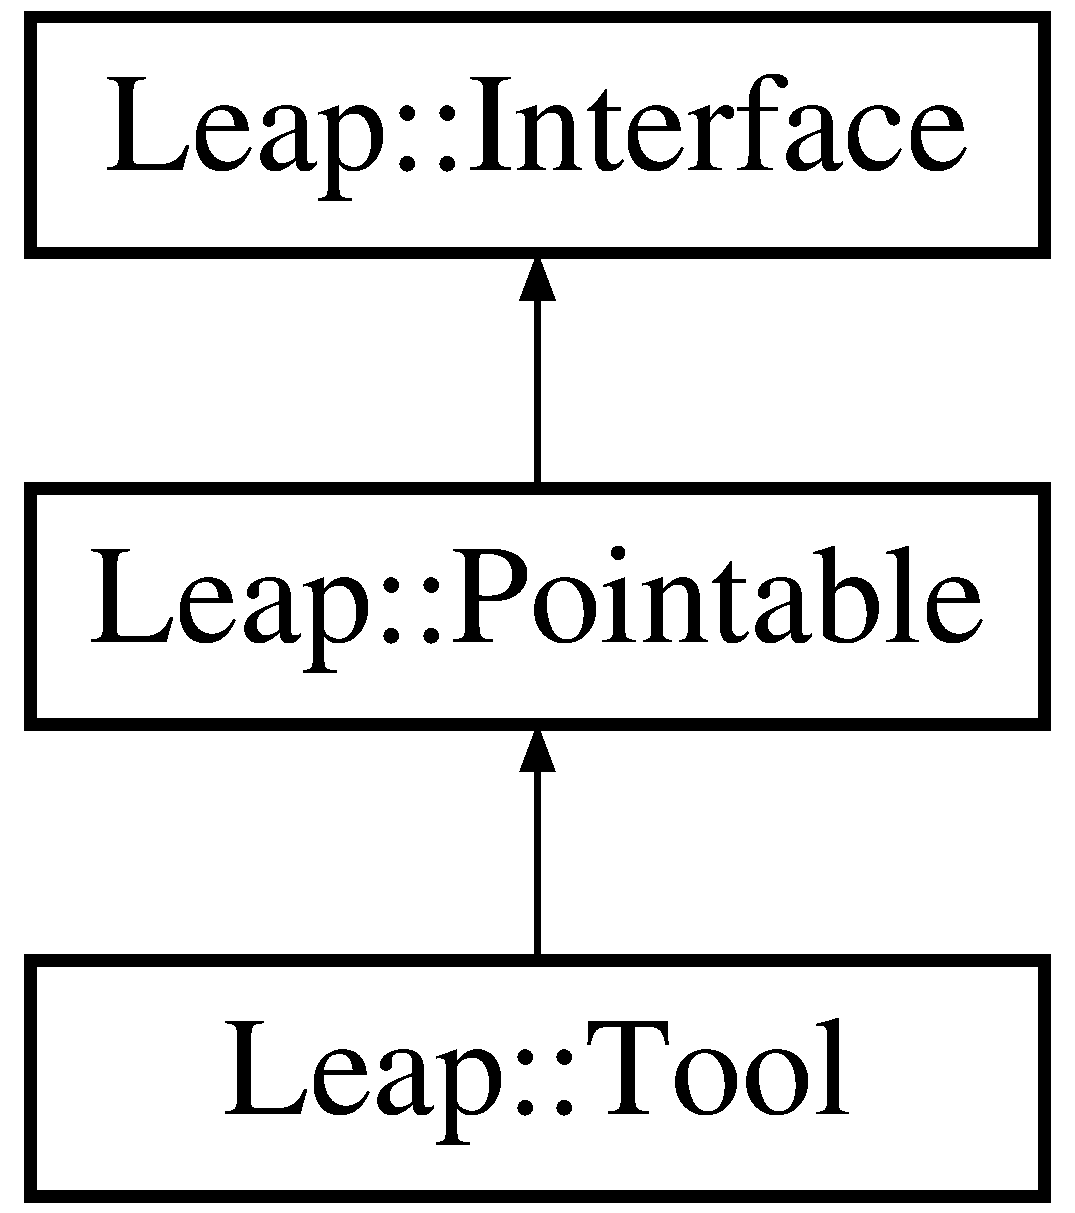
\includegraphics[height=3.000000cm]{class_leap_1_1_tool}
\end{center}
\end{figure}
\subsection*{Public Member Functions}
\begin{DoxyCompactItemize}
\item 
\hypertarget{class_leap_1_1_tool_a856522513b4dbf3ef4e2a9a9667f5735}{{\bfseries Tool} (Tool\+Implementation $\ast$)}\label{class_leap_1_1_tool_a856522513b4dbf3ef4e2a9a9667f5735}

\item 
L\+E\+A\+P\+\_\+\+E\+X\+P\+O\+R\+T \hyperlink{class_leap_1_1_tool_a6debbdfc14096362bf32228ba3e5c72f}{Tool} ()
\item 
L\+E\+A\+P\+\_\+\+E\+X\+P\+O\+R\+T \hyperlink{class_leap_1_1_tool_a6dfea4c318389bcc6d1ef373d7a4432e}{Tool} (const \hyperlink{class_leap_1_1_pointable}{Pointable} \&)
\item 
L\+E\+A\+P\+\_\+\+E\+X\+P\+O\+R\+T std\+::string \hyperlink{class_leap_1_1_tool_ad3dbe186886683f46996fd0c8ca5a940}{to\+String} () const 
\end{DoxyCompactItemize}
\subsection*{Static Public Member Functions}
\begin{DoxyCompactItemize}
\item 
static L\+E\+A\+P\+\_\+\+E\+X\+P\+O\+R\+T const \hyperlink{class_leap_1_1_tool}{Tool} \& \hyperlink{class_leap_1_1_tool_af47b7fe3674536f265470e7ab3467ef1}{invalid} ()
\end{DoxyCompactItemize}
\subsection*{Additional Inherited Members}


\subsection{Detailed Description}
The \hyperlink{class_leap_1_1_tool}{Tool} class represents a tracked tool.

Tools are \hyperlink{class_leap_1_1_pointable}{Pointable} objects that the Leap Motion software has classified as a tool. Tools are longer, thinner, and straighter than a typical finger. Get valid \hyperlink{class_leap_1_1_tool}{Tool} objects from a \hyperlink{class_leap_1_1_frame}{Frame} or a \hyperlink{class_leap_1_1_hand}{Hand} object.

Tools may reference a hand, but unlike fingers they are not permanently associated. Instead, a tool can be transferred between hands while keeping the same I\+D.



Note that \hyperlink{class_leap_1_1_tool}{Tool} objects can be invalid, which means that they do not contain valid tracking data and do not correspond to a physical tool. Invalid \hyperlink{class_leap_1_1_tool}{Tool} objects can be the result of asking for a \hyperlink{class_leap_1_1_tool}{Tool} object using an I\+D from an earlier frame when no \hyperlink{class_leap_1_1_tool}{Tool} objects with that I\+D exist in the current frame. A \hyperlink{class_leap_1_1_tool}{Tool} object created from the \hyperlink{class_leap_1_1_tool}{Tool} constructor is also invalid. Test for validity with the \hyperlink{class_leap_1_1_pointable_a124f21a619df4fb338d1ce8a7a6d3341}{Tool\+::is\+Valid()} function. \begin{DoxySince}{Since}
1.\+0 
\end{DoxySince}


\subsection{Constructor \& Destructor Documentation}
\hypertarget{class_leap_1_1_tool_a6debbdfc14096362bf32228ba3e5c72f}{\index{Leap\+::\+Tool@{Leap\+::\+Tool}!Tool@{Tool}}
\index{Tool@{Tool}!Leap\+::\+Tool@{Leap\+::\+Tool}}
\subsubsection[{Tool}]{\setlength{\rightskip}{0pt plus 5cm}L\+E\+A\+P\+\_\+\+E\+X\+P\+O\+R\+T Leap\+::\+Tool\+::\+Tool (
\begin{DoxyParamCaption}
{}
\end{DoxyParamCaption}
)}}\label{class_leap_1_1_tool_a6debbdfc14096362bf32228ba3e5c72f}
Constructs a \hyperlink{class_leap_1_1_tool}{Tool} object.

An uninitialized tool is considered invalid. Get valid \hyperlink{class_leap_1_1_tool}{Tool} objects from a \hyperlink{class_leap_1_1_frame}{Frame} or a \hyperlink{class_leap_1_1_hand}{Hand} object. \begin{DoxySince}{Since}
1.\+0 
\end{DoxySince}
\hypertarget{class_leap_1_1_tool_a6dfea4c318389bcc6d1ef373d7a4432e}{\index{Leap\+::\+Tool@{Leap\+::\+Tool}!Tool@{Tool}}
\index{Tool@{Tool}!Leap\+::\+Tool@{Leap\+::\+Tool}}
\subsubsection[{Tool}]{\setlength{\rightskip}{0pt plus 5cm}L\+E\+A\+P\+\_\+\+E\+X\+P\+O\+R\+T Leap\+::\+Tool\+::\+Tool (
\begin{DoxyParamCaption}
\item[{const {\bf Pointable} \&}]{}
\end{DoxyParamCaption}
)\hspace{0.3cm}{\ttfamily [explicit]}}}\label{class_leap_1_1_tool_a6dfea4c318389bcc6d1ef373d7a4432e}
If the specified \hyperlink{class_leap_1_1_pointable}{Pointable} object represents a tool, creates a copy of it as a \hyperlink{class_leap_1_1_tool}{Tool} object; otherwise, creates an invalid \hyperlink{class_leap_1_1_tool}{Tool} object. \begin{DoxySince}{Since}
1.\+0 
\end{DoxySince}


\subsection{Member Function Documentation}
\hypertarget{class_leap_1_1_tool_af47b7fe3674536f265470e7ab3467ef1}{\index{Leap\+::\+Tool@{Leap\+::\+Tool}!invalid@{invalid}}
\index{invalid@{invalid}!Leap\+::\+Tool@{Leap\+::\+Tool}}
\subsubsection[{invalid}]{\setlength{\rightskip}{0pt plus 5cm}static L\+E\+A\+P\+\_\+\+E\+X\+P\+O\+R\+T const {\bf Tool}\& Leap\+::\+Tool\+::invalid (
\begin{DoxyParamCaption}
{}
\end{DoxyParamCaption}
)\hspace{0.3cm}{\ttfamily [static]}}}\label{class_leap_1_1_tool_af47b7fe3674536f265470e7ab3467ef1}
Returns an invalid \hyperlink{class_leap_1_1_tool}{Tool} object.

You can use the instance returned by this function in comparisons testing whether a given \hyperlink{class_leap_1_1_tool}{Tool} instance is valid or invalid. (You can also use the \hyperlink{class_leap_1_1_pointable_a124f21a619df4fb338d1ce8a7a6d3341}{Tool\+::is\+Valid()} function.)

\begin{DoxyReturn}{Returns}
The invalid \hyperlink{class_leap_1_1_tool}{Tool} instance. 
\end{DoxyReturn}
\begin{DoxySince}{Since}
1.\+0 
\end{DoxySince}
\hypertarget{class_leap_1_1_tool_ad3dbe186886683f46996fd0c8ca5a940}{\index{Leap\+::\+Tool@{Leap\+::\+Tool}!to\+String@{to\+String}}
\index{to\+String@{to\+String}!Leap\+::\+Tool@{Leap\+::\+Tool}}
\subsubsection[{to\+String}]{\setlength{\rightskip}{0pt plus 5cm}L\+E\+A\+P\+\_\+\+E\+X\+P\+O\+R\+T std\+::string Leap\+::\+Tool\+::to\+String (
\begin{DoxyParamCaption}
{}
\end{DoxyParamCaption}
) const}}\label{class_leap_1_1_tool_ad3dbe186886683f46996fd0c8ca5a940}
A string containing a brief, human readable description of the \hyperlink{class_leap_1_1_tool}{Tool} object.

\begin{DoxyReturn}{Returns}
A description of the \hyperlink{class_leap_1_1_tool}{Tool} object as a string. 
\end{DoxyReturn}
\begin{DoxySince}{Since}
1.\+0 
\end{DoxySince}


The documentation for this class was generated from the following file\+:\begin{DoxyCompactItemize}
\item 
Interface\+Managers/Leap.\+h\end{DoxyCompactItemize}

\hypertarget{class_leap_1_1_tool_list}{\section{Leap\+:\+:Tool\+List Class Reference}
\label{class_leap_1_1_tool_list}\index{Leap\+::\+Tool\+List@{Leap\+::\+Tool\+List}}
}


{\ttfamily \#include $<$Leap.\+h$>$}

Inheritance diagram for Leap\+:\+:Tool\+List\+:\begin{figure}[H]
\begin{center}
\leavevmode
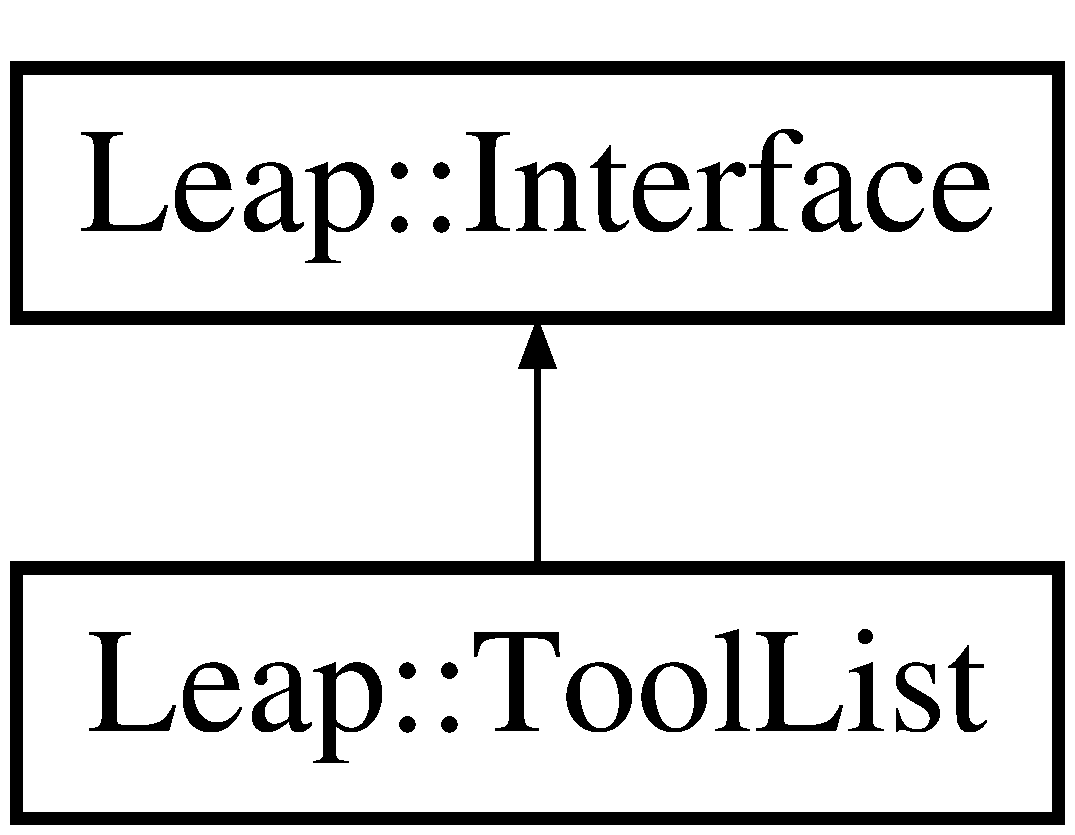
\includegraphics[height=2.000000cm]{class_leap_1_1_tool_list}
\end{center}
\end{figure}
\subsection*{Public Types}
\begin{DoxyCompactItemize}
\item 
typedef \hyperlink{class_leap_1_1_const_list_iterator}{Const\+List\+Iterator}\\*
$<$ \hyperlink{class_leap_1_1_tool_list}{Tool\+List}, \hyperlink{class_leap_1_1_tool}{Tool} $>$ \hyperlink{class_leap_1_1_tool_list_a7f52ee5561016e8d42512e2adbc820de}{const\+\_\+iterator}
\end{DoxyCompactItemize}
\subsection*{Public Member Functions}
\begin{DoxyCompactItemize}
\item 
\hypertarget{class_leap_1_1_tool_list_a28459f829ceca1ac6edfe5dd5f0a73d5}{{\bfseries Tool\+List} (const \hyperlink{class_leap_1_1_list_base_implementation}{List\+Base\+Implementation}$<$ \hyperlink{class_leap_1_1_tool}{Tool} $>$ \&)}\label{class_leap_1_1_tool_list_a28459f829ceca1ac6edfe5dd5f0a73d5}

\item 
L\+E\+A\+P\+\_\+\+E\+X\+P\+O\+R\+T \hyperlink{class_leap_1_1_tool_list_a3ee8e7e7b50f92b9d31ad31e7fd55c2e}{Tool\+List} ()
\item 
L\+E\+A\+P\+\_\+\+E\+X\+P\+O\+R\+T int \hyperlink{class_leap_1_1_tool_list_a385325630ca55bfcad1e5b06237fbcbb}{count} () const 
\item 
L\+E\+A\+P\+\_\+\+E\+X\+P\+O\+R\+T bool \hyperlink{class_leap_1_1_tool_list_a96832d98859addb02813fcba73cd1d2e}{is\+Empty} () const 
\item 
L\+E\+A\+P\+\_\+\+E\+X\+P\+O\+R\+T \hyperlink{class_leap_1_1_tool}{Tool} \hyperlink{class_leap_1_1_tool_list_ad9cb174832fe6d8a10592bced6ea2cb1}{operator\mbox{[}$\,$\mbox{]}} (int index) const 
\item 
L\+E\+A\+P\+\_\+\+E\+X\+P\+O\+R\+T \hyperlink{class_leap_1_1_tool_list}{Tool\+List} \& \hyperlink{class_leap_1_1_tool_list_a384adf507eeb1cfacc5aaa71a38ca452}{append} (const \hyperlink{class_leap_1_1_tool_list}{Tool\+List} \&other)
\item 
L\+E\+A\+P\+\_\+\+E\+X\+P\+O\+R\+T \hyperlink{class_leap_1_1_tool}{Tool} \hyperlink{class_leap_1_1_tool_list_ac22bad454f5086fcea7cc75de2a2cb7c}{leftmost} () const 
\item 
L\+E\+A\+P\+\_\+\+E\+X\+P\+O\+R\+T \hyperlink{class_leap_1_1_tool}{Tool} \hyperlink{class_leap_1_1_tool_list_abdd27a1e89f90a33af077f8827210487}{rightmost} () const 
\item 
L\+E\+A\+P\+\_\+\+E\+X\+P\+O\+R\+T \hyperlink{class_leap_1_1_tool}{Tool} \hyperlink{class_leap_1_1_tool_list_a6641d8cba062215cbf38982015145ffe}{frontmost} () const 
\item 
L\+E\+A\+P\+\_\+\+E\+X\+P\+O\+R\+T \hyperlink{class_leap_1_1_tool_list_a7f52ee5561016e8d42512e2adbc820de}{const\+\_\+iterator} \hyperlink{class_leap_1_1_tool_list_abf5d56a04145998fc85a7be12898f210}{begin} () const 
\item 
L\+E\+A\+P\+\_\+\+E\+X\+P\+O\+R\+T \hyperlink{class_leap_1_1_tool_list_a7f52ee5561016e8d42512e2adbc820de}{const\+\_\+iterator} \hyperlink{class_leap_1_1_tool_list_a42a50495878c9c4824f78391f6de637c}{end} () const 
\end{DoxyCompactItemize}
\subsection*{Additional Inherited Members}


\subsection{Detailed Description}
The \hyperlink{class_leap_1_1_tool_list}{Tool\+List} class represents a list of \hyperlink{class_leap_1_1_tool}{Tool} objects.

Get a \hyperlink{class_leap_1_1_tool_list}{Tool\+List} object by calling \hyperlink{class_leap_1_1_frame_abf81ff857abdd1cc9c2ccb889eb1c6e3}{Frame\+::tools()}. \begin{DoxySince}{Since}
1.\+0 
\end{DoxySince}


\subsection{Member Typedef Documentation}
\hypertarget{class_leap_1_1_tool_list_a7f52ee5561016e8d42512e2adbc820de}{\index{Leap\+::\+Tool\+List@{Leap\+::\+Tool\+List}!const\+\_\+iterator@{const\+\_\+iterator}}
\index{const\+\_\+iterator@{const\+\_\+iterator}!Leap\+::\+Tool\+List@{Leap\+::\+Tool\+List}}
\subsubsection[{const\+\_\+iterator}]{\setlength{\rightskip}{0pt plus 5cm}typedef {\bf Const\+List\+Iterator}$<${\bf Tool\+List}, {\bf Tool}$>$ {\bf Leap\+::\+Tool\+List\+::const\+\_\+iterator}}}\label{class_leap_1_1_tool_list_a7f52ee5561016e8d42512e2adbc820de}
A C++ iterator type for \hyperlink{class_leap_1_1_tool_list}{Tool\+List} objects. \begin{DoxySince}{Since}
1.\+0 
\end{DoxySince}


\subsection{Constructor \& Destructor Documentation}
\hypertarget{class_leap_1_1_tool_list_a3ee8e7e7b50f92b9d31ad31e7fd55c2e}{\index{Leap\+::\+Tool\+List@{Leap\+::\+Tool\+List}!Tool\+List@{Tool\+List}}
\index{Tool\+List@{Tool\+List}!Leap\+::\+Tool\+List@{Leap\+::\+Tool\+List}}
\subsubsection[{Tool\+List}]{\setlength{\rightskip}{0pt plus 5cm}L\+E\+A\+P\+\_\+\+E\+X\+P\+O\+R\+T Leap\+::\+Tool\+List\+::\+Tool\+List (
\begin{DoxyParamCaption}
{}
\end{DoxyParamCaption}
)}}\label{class_leap_1_1_tool_list_a3ee8e7e7b50f92b9d31ad31e7fd55c2e}
Constructs an empty list of tools. \begin{DoxySince}{Since}
1.\+0 
\end{DoxySince}


\subsection{Member Function Documentation}
\hypertarget{class_leap_1_1_tool_list_a384adf507eeb1cfacc5aaa71a38ca452}{\index{Leap\+::\+Tool\+List@{Leap\+::\+Tool\+List}!append@{append}}
\index{append@{append}!Leap\+::\+Tool\+List@{Leap\+::\+Tool\+List}}
\subsubsection[{append}]{\setlength{\rightskip}{0pt plus 5cm}L\+E\+A\+P\+\_\+\+E\+X\+P\+O\+R\+T {\bf Tool\+List}\& Leap\+::\+Tool\+List\+::append (
\begin{DoxyParamCaption}
\item[{const {\bf Tool\+List} \&}]{other}
\end{DoxyParamCaption}
)}}\label{class_leap_1_1_tool_list_a384adf507eeb1cfacc5aaa71a38ca452}
Appends the members of the specifed \hyperlink{class_leap_1_1_tool_list}{Tool\+List} to this \hyperlink{class_leap_1_1_tool_list}{Tool\+List}. 
\begin{DoxyParams}{Parameters}
{\em other} & A \hyperlink{class_leap_1_1_tool_list}{Tool\+List} object containing \hyperlink{class_leap_1_1_tool}{Tool} objects to append to the end of this \hyperlink{class_leap_1_1_tool_list}{Tool\+List}. \\
\hline
\end{DoxyParams}
\begin{DoxySince}{Since}
1.\+0 
\end{DoxySince}
\hypertarget{class_leap_1_1_tool_list_abf5d56a04145998fc85a7be12898f210}{\index{Leap\+::\+Tool\+List@{Leap\+::\+Tool\+List}!begin@{begin}}
\index{begin@{begin}!Leap\+::\+Tool\+List@{Leap\+::\+Tool\+List}}
\subsubsection[{begin}]{\setlength{\rightskip}{0pt plus 5cm}L\+E\+A\+P\+\_\+\+E\+X\+P\+O\+R\+T {\bf const\+\_\+iterator} Leap\+::\+Tool\+List\+::begin (
\begin{DoxyParamCaption}
{}
\end{DoxyParamCaption}
) const}}\label{class_leap_1_1_tool_list_abf5d56a04145998fc85a7be12898f210}
The C++ iterator set to the beginning of this \hyperlink{class_leap_1_1_tool_list}{Tool\+List}. \begin{DoxySince}{Since}
1.\+0 
\end{DoxySince}
\hypertarget{class_leap_1_1_tool_list_a385325630ca55bfcad1e5b06237fbcbb}{\index{Leap\+::\+Tool\+List@{Leap\+::\+Tool\+List}!count@{count}}
\index{count@{count}!Leap\+::\+Tool\+List@{Leap\+::\+Tool\+List}}
\subsubsection[{count}]{\setlength{\rightskip}{0pt plus 5cm}L\+E\+A\+P\+\_\+\+E\+X\+P\+O\+R\+T int Leap\+::\+Tool\+List\+::count (
\begin{DoxyParamCaption}
{}
\end{DoxyParamCaption}
) const}}\label{class_leap_1_1_tool_list_a385325630ca55bfcad1e5b06237fbcbb}
Returns the number of tools in this list. \begin{DoxyReturn}{Returns}
The number of tools in this list. 
\end{DoxyReturn}
\begin{DoxySince}{Since}
1.\+0 
\end{DoxySince}
\hypertarget{class_leap_1_1_tool_list_a42a50495878c9c4824f78391f6de637c}{\index{Leap\+::\+Tool\+List@{Leap\+::\+Tool\+List}!end@{end}}
\index{end@{end}!Leap\+::\+Tool\+List@{Leap\+::\+Tool\+List}}
\subsubsection[{end}]{\setlength{\rightskip}{0pt plus 5cm}L\+E\+A\+P\+\_\+\+E\+X\+P\+O\+R\+T {\bf const\+\_\+iterator} Leap\+::\+Tool\+List\+::end (
\begin{DoxyParamCaption}
{}
\end{DoxyParamCaption}
) const}}\label{class_leap_1_1_tool_list_a42a50495878c9c4824f78391f6de637c}
The C++ iterator set to the end of this \hyperlink{class_leap_1_1_tool_list}{Tool\+List}. \begin{DoxySince}{Since}
1.\+0 
\end{DoxySince}
\hypertarget{class_leap_1_1_tool_list_a6641d8cba062215cbf38982015145ffe}{\index{Leap\+::\+Tool\+List@{Leap\+::\+Tool\+List}!frontmost@{frontmost}}
\index{frontmost@{frontmost}!Leap\+::\+Tool\+List@{Leap\+::\+Tool\+List}}
\subsubsection[{frontmost}]{\setlength{\rightskip}{0pt plus 5cm}L\+E\+A\+P\+\_\+\+E\+X\+P\+O\+R\+T {\bf Tool} Leap\+::\+Tool\+List\+::frontmost (
\begin{DoxyParamCaption}
{}
\end{DoxyParamCaption}
) const}}\label{class_leap_1_1_tool_list_a6641d8cba062215cbf38982015145ffe}
The member of the list that is farthest to the front within the standard Leap Motion frame of reference (i.\+e has the smallest Z coordinate).

\begin{DoxyReturn}{Returns}
The frontmost tool, or invalid if list is empty. 
\end{DoxyReturn}
\begin{DoxySince}{Since}
1.\+0 
\end{DoxySince}
\hypertarget{class_leap_1_1_tool_list_a96832d98859addb02813fcba73cd1d2e}{\index{Leap\+::\+Tool\+List@{Leap\+::\+Tool\+List}!is\+Empty@{is\+Empty}}
\index{is\+Empty@{is\+Empty}!Leap\+::\+Tool\+List@{Leap\+::\+Tool\+List}}
\subsubsection[{is\+Empty}]{\setlength{\rightskip}{0pt plus 5cm}L\+E\+A\+P\+\_\+\+E\+X\+P\+O\+R\+T bool Leap\+::\+Tool\+List\+::is\+Empty (
\begin{DoxyParamCaption}
{}
\end{DoxyParamCaption}
) const}}\label{class_leap_1_1_tool_list_a96832d98859addb02813fcba73cd1d2e}
Reports whether the list is empty. \begin{DoxyReturn}{Returns}
True, if the list has no members. 
\end{DoxyReturn}
\begin{DoxySince}{Since}
1.\+0 
\end{DoxySince}
\hypertarget{class_leap_1_1_tool_list_ac22bad454f5086fcea7cc75de2a2cb7c}{\index{Leap\+::\+Tool\+List@{Leap\+::\+Tool\+List}!leftmost@{leftmost}}
\index{leftmost@{leftmost}!Leap\+::\+Tool\+List@{Leap\+::\+Tool\+List}}
\subsubsection[{leftmost}]{\setlength{\rightskip}{0pt plus 5cm}L\+E\+A\+P\+\_\+\+E\+X\+P\+O\+R\+T {\bf Tool} Leap\+::\+Tool\+List\+::leftmost (
\begin{DoxyParamCaption}
{}
\end{DoxyParamCaption}
) const}}\label{class_leap_1_1_tool_list_ac22bad454f5086fcea7cc75de2a2cb7c}
The member of the list that is farthest to the left within the standard Leap Motion frame of reference (i.\+e has the smallest X coordinate).

\begin{DoxyReturn}{Returns}
The leftmost tool, or invalid if list is empty. 
\end{DoxyReturn}
\begin{DoxySince}{Since}
1.\+0 
\end{DoxySince}
\hypertarget{class_leap_1_1_tool_list_ad9cb174832fe6d8a10592bced6ea2cb1}{\index{Leap\+::\+Tool\+List@{Leap\+::\+Tool\+List}!operator\mbox{[}$\,$\mbox{]}@{operator[]}}
\index{operator\mbox{[}$\,$\mbox{]}@{operator[]}!Leap\+::\+Tool\+List@{Leap\+::\+Tool\+List}}
\subsubsection[{operator[]}]{\setlength{\rightskip}{0pt plus 5cm}L\+E\+A\+P\+\_\+\+E\+X\+P\+O\+R\+T {\bf Tool} Leap\+::\+Tool\+List\+::operator\mbox{[}$\,$\mbox{]} (
\begin{DoxyParamCaption}
\item[{int}]{index}
\end{DoxyParamCaption}
) const}}\label{class_leap_1_1_tool_list_ad9cb174832fe6d8a10592bced6ea2cb1}
Access a list member by its position in the list. 
\begin{DoxyParams}{Parameters}
{\em index} & The zero-\/based list position index. \\
\hline
\end{DoxyParams}
\begin{DoxyReturn}{Returns}
The \hyperlink{class_leap_1_1_tool}{Tool} object at the specified index. 
\end{DoxyReturn}
\begin{DoxySince}{Since}
1.\+0 
\end{DoxySince}
\hypertarget{class_leap_1_1_tool_list_abdd27a1e89f90a33af077f8827210487}{\index{Leap\+::\+Tool\+List@{Leap\+::\+Tool\+List}!rightmost@{rightmost}}
\index{rightmost@{rightmost}!Leap\+::\+Tool\+List@{Leap\+::\+Tool\+List}}
\subsubsection[{rightmost}]{\setlength{\rightskip}{0pt plus 5cm}L\+E\+A\+P\+\_\+\+E\+X\+P\+O\+R\+T {\bf Tool} Leap\+::\+Tool\+List\+::rightmost (
\begin{DoxyParamCaption}
{}
\end{DoxyParamCaption}
) const}}\label{class_leap_1_1_tool_list_abdd27a1e89f90a33af077f8827210487}
The member of the list that is farthest to the right within the standard Leap Motion frame of reference (i.\+e has the largest X coordinate).

\begin{DoxyReturn}{Returns}
The rightmost tool, or invalid if list is empty. 
\end{DoxyReturn}
\begin{DoxySince}{Since}
1.\+0 
\end{DoxySince}


The documentation for this class was generated from the following file\+:\begin{DoxyCompactItemize}
\item 
Interface\+Managers/Leap.\+h\end{DoxyCompactItemize}

\hypertarget{class_trial_data}{\section{Trial\+Data Class Reference}
\label{class_trial_data}\index{Trial\+Data@{Trial\+Data}}
}
\subsection*{Public Member Functions}
\begin{DoxyCompactItemize}
\item 
\hypertarget{class_trial_data_ab61aef92abe489ef01ad048417d357af}{\hyperlink{class_trial_data_ab61aef92abe489ef01ad048417d357af}{Trial\+Data} ()}\label{class_trial_data_ab61aef92abe489ef01ad048417d357af}

\begin{DoxyCompactList}\small\item\em Constructor for \hyperlink{class_trial_data}{Trial\+Data} object \hyperlink{class_trial_data}{Trial\+Data} holds all data for the entire trial of Simon. It's flushed and reinitialized before each trial. \end{DoxyCompactList}\item 
\hyperlink{class_game_data}{Game\+Data} $\ast$ \hyperlink{class_trial_data_ab82ebe277cd6251973fa9efdd09b063d}{get\+Game} (int index)
\begin{DoxyCompactList}\small\item\em Fetch a game from the internal list. \end{DoxyCompactList}\item 
int \hyperlink{class_trial_data_aa66d11b4deef49c0abb14b13047663a9}{get\+Number\+Games} ()
\begin{DoxyCompactList}\small\item\em The number of games in the internal game array. \end{DoxyCompactList}\item 
void \hyperlink{class_trial_data_a813986c375dabdbf0efa382213604e84}{set\+P\+I\+D} (std\+::string pid)
\begin{DoxyCompactList}\small\item\em Sets the subject's participant I\+D in the record. \end{DoxyCompactList}\item 
void \hyperlink{class_trial_data_accfa4cd37e47a847562793831e7db5a7}{set\+Gender} (bool gender)
\begin{DoxyCompactList}\small\item\em Sets the subject's gender in the record. \end{DoxyCompactList}\item 
void \hyperlink{class_trial_data_acd2c2aedea1718872165ce0bf0df6029}{set\+Age} (int age)
\begin{DoxyCompactList}\small\item\em Sets the subject's age in the record. \end{DoxyCompactList}\item 
void \hyperlink{class_trial_data_afdedfaa564bfe3ca1529614c32acef37}{set\+Out\+File} (std\+::string out\+File)
\begin{DoxyCompactList}\small\item\em Sets the destanation location for the session report. No access testing is performed. \end{DoxyCompactList}\item 
\hypertarget{class_trial_data_ac0a8256a5f04818711c72ff88223839c}{void \hyperlink{class_trial_data_ac0a8256a5f04818711c72ff88223839c}{add\+Game} ()}\label{class_trial_data_ac0a8256a5f04818711c72ff88223839c}

\begin{DoxyCompactList}\small\item\em Appends a game to the list of games to be played. \end{DoxyCompactList}\item 
void \hyperlink{class_trial_data_af3a0f221160d45fd6d28168235ed3d5a}{add\+Game} (\hyperlink{class_game_data}{Game\+Data} gd)
\begin{DoxyCompactList}\small\item\em Appends a C\+U\+S\+T\+O\+M game to the list of games to be played. \end{DoxyCompactList}\item 
void \hyperlink{class_trial_data_a2af0b8b20496f6daf919e52e103da7de}{swap\+Games} (int index1, int index2)
\begin{DoxyCompactList}\small\item\em Swap Games in a list by index. \end{DoxyCompactList}\item 
void \hyperlink{class_trial_data_a0c941bb4edc8d98ed0883650a1d7f502}{remove\+Game} (int index)
\begin{DoxyCompactList}\small\item\em Removes a game from the running list. \end{DoxyCompactList}\item 
Error\+Type \hyperlink{class_trial_data_aa18ad64f9b9b6b980fec9ab3e1455559}{write\+C\+S\+V} ()
\begin{DoxyCompactList}\small\item\em Writes all current games out to memory. \end{DoxyCompactList}\end{DoxyCompactItemize}
\subsection*{Static Public Member Functions}
\begin{DoxyCompactItemize}
\item 
static \hyperlink{class_trial_data}{Trial\+Data} $\ast$ \hyperlink{class_trial_data_a86a08d5deb1ae938e007667b8cd4a167}{get\+Current\+Trial} ()
\begin{DoxyCompactList}\small\item\em Grabs a copy of the currently active trial\+Data. \end{DoxyCompactList}\item 
\hypertarget{class_trial_data_a51db8ba5ec8a1e8f0107166db54dac18}{static void \hyperlink{class_trial_data_a51db8ba5ec8a1e8f0107166db54dac18}{new\+Trial} ()}\label{class_trial_data_a51db8ba5ec8a1e8f0107166db54dac18}

\begin{DoxyCompactList}\small\item\em Resets all gathered data\+: user metrics, times, quadrants, and so on. \end{DoxyCompactList}\end{DoxyCompactItemize}


\subsection{Member Function Documentation}
\hypertarget{class_trial_data_af3a0f221160d45fd6d28168235ed3d5a}{\index{Trial\+Data@{Trial\+Data}!add\+Game@{add\+Game}}
\index{add\+Game@{add\+Game}!Trial\+Data@{Trial\+Data}}
\subsubsection[{add\+Game}]{\setlength{\rightskip}{0pt plus 5cm}void Trial\+Data\+::add\+Game (
\begin{DoxyParamCaption}
\item[{{\bf Game\+Data}}]{gd}
\end{DoxyParamCaption}
)}}\label{class_trial_data_af3a0f221160d45fd6d28168235ed3d5a}


Appends a C\+U\+S\+T\+O\+M game to the list of games to be played. 


\begin{DoxyParams}{Parameters}
{\em gd} & The game to append to the list of games. \\
\hline
\end{DoxyParams}
\hypertarget{class_trial_data_a86a08d5deb1ae938e007667b8cd4a167}{\index{Trial\+Data@{Trial\+Data}!get\+Current\+Trial@{get\+Current\+Trial}}
\index{get\+Current\+Trial@{get\+Current\+Trial}!Trial\+Data@{Trial\+Data}}
\subsubsection[{get\+Current\+Trial}]{\setlength{\rightskip}{0pt plus 5cm}{\bf Trial\+Data} $\ast$ Trial\+Data\+::get\+Current\+Trial (
\begin{DoxyParamCaption}
{}
\end{DoxyParamCaption}
)\hspace{0.3cm}{\ttfamily [static]}}}\label{class_trial_data_a86a08d5deb1ae938e007667b8cd4a167}


Grabs a copy of the currently active trial\+Data. 

\begin{DoxyReturn}{Returns}
A reference to the active \hyperlink{class_trial_data}{Trial\+Data} \hyperlink{class_trial_data}{Trial\+Data} is a singleton through the entire game. get\+Current\+Trial grabs a pointer to the singleton. 
\end{DoxyReturn}
\hypertarget{class_trial_data_ab82ebe277cd6251973fa9efdd09b063d}{\index{Trial\+Data@{Trial\+Data}!get\+Game@{get\+Game}}
\index{get\+Game@{get\+Game}!Trial\+Data@{Trial\+Data}}
\subsubsection[{get\+Game}]{\setlength{\rightskip}{0pt plus 5cm}{\bf Game\+Data} $\ast$ Trial\+Data\+::get\+Game (
\begin{DoxyParamCaption}
\item[{int}]{index}
\end{DoxyParamCaption}
)}}\label{class_trial_data_ab82ebe277cd6251973fa9efdd09b063d}


Fetch a game from the internal list. 

\begin{DoxyReturn}{Returns}
A reference to the game 
\end{DoxyReturn}

\begin{DoxyParams}{Parameters}
{\em index} & The array index of the game to fetch. \\
\hline
\end{DoxyParams}
\hypertarget{class_trial_data_aa66d11b4deef49c0abb14b13047663a9}{\index{Trial\+Data@{Trial\+Data}!get\+Number\+Games@{get\+Number\+Games}}
\index{get\+Number\+Games@{get\+Number\+Games}!Trial\+Data@{Trial\+Data}}
\subsubsection[{get\+Number\+Games}]{\setlength{\rightskip}{0pt plus 5cm}int Trial\+Data\+::get\+Number\+Games (
\begin{DoxyParamCaption}
{}
\end{DoxyParamCaption}
)}}\label{class_trial_data_aa66d11b4deef49c0abb14b13047663a9}


The number of games in the internal game array. 

\begin{DoxyReturn}{Returns}
Number of games in the array. 
\end{DoxyReturn}
\hypertarget{class_trial_data_a0c941bb4edc8d98ed0883650a1d7f502}{\index{Trial\+Data@{Trial\+Data}!remove\+Game@{remove\+Game}}
\index{remove\+Game@{remove\+Game}!Trial\+Data@{Trial\+Data}}
\subsubsection[{remove\+Game}]{\setlength{\rightskip}{0pt plus 5cm}void Trial\+Data\+::remove\+Game (
\begin{DoxyParamCaption}
\item[{int}]{index}
\end{DoxyParamCaption}
)}}\label{class_trial_data_a0c941bb4edc8d98ed0883650a1d7f502}


Removes a game from the running list. 


\begin{DoxyParams}{Parameters}
{\em index} & The index of the game to remove \\
\hline
\end{DoxyParams}
\hypertarget{class_trial_data_acd2c2aedea1718872165ce0bf0df6029}{\index{Trial\+Data@{Trial\+Data}!set\+Age@{set\+Age}}
\index{set\+Age@{set\+Age}!Trial\+Data@{Trial\+Data}}
\subsubsection[{set\+Age}]{\setlength{\rightskip}{0pt plus 5cm}void Trial\+Data\+::set\+Age (
\begin{DoxyParamCaption}
\item[{int}]{age}
\end{DoxyParamCaption}
)}}\label{class_trial_data_acd2c2aedea1718872165ce0bf0df6029}


Sets the subject's age in the record. 


\begin{DoxyParams}{Parameters}
{\em age} & The subject's age \\
\hline
\end{DoxyParams}
\hypertarget{class_trial_data_accfa4cd37e47a847562793831e7db5a7}{\index{Trial\+Data@{Trial\+Data}!set\+Gender@{set\+Gender}}
\index{set\+Gender@{set\+Gender}!Trial\+Data@{Trial\+Data}}
\subsubsection[{set\+Gender}]{\setlength{\rightskip}{0pt plus 5cm}void Trial\+Data\+::set\+Gender (
\begin{DoxyParamCaption}
\item[{bool}]{gender}
\end{DoxyParamCaption}
)}}\label{class_trial_data_accfa4cd37e47a847562793831e7db5a7}


Sets the subject's gender in the record. 


\begin{DoxyParams}{Parameters}
{\em gender} & The subject's gender \\
\hline
\end{DoxyParams}
\hypertarget{class_trial_data_afdedfaa564bfe3ca1529614c32acef37}{\index{Trial\+Data@{Trial\+Data}!set\+Out\+File@{set\+Out\+File}}
\index{set\+Out\+File@{set\+Out\+File}!Trial\+Data@{Trial\+Data}}
\subsubsection[{set\+Out\+File}]{\setlength{\rightskip}{0pt plus 5cm}void Trial\+Data\+::set\+Out\+File (
\begin{DoxyParamCaption}
\item[{std\+::string}]{out\+File}
\end{DoxyParamCaption}
)}}\label{class_trial_data_afdedfaa564bfe3ca1529614c32acef37}


Sets the destanation location for the session report. No access testing is performed. 


\begin{DoxyParams}{Parameters}
{\em out\+File} & The path to the file to write, as a string. \\
\hline
\end{DoxyParams}
\hypertarget{class_trial_data_a813986c375dabdbf0efa382213604e84}{\index{Trial\+Data@{Trial\+Data}!set\+P\+I\+D@{set\+P\+I\+D}}
\index{set\+P\+I\+D@{set\+P\+I\+D}!Trial\+Data@{Trial\+Data}}
\subsubsection[{set\+P\+I\+D}]{\setlength{\rightskip}{0pt plus 5cm}void Trial\+Data\+::set\+P\+I\+D (
\begin{DoxyParamCaption}
\item[{std\+::string}]{pid}
\end{DoxyParamCaption}
)}}\label{class_trial_data_a813986c375dabdbf0efa382213604e84}


Sets the subject's participant I\+D in the record. 


\begin{DoxyParams}{Parameters}
{\em pid} & The subject's participant I\+D \\
\hline
\end{DoxyParams}
\hypertarget{class_trial_data_a2af0b8b20496f6daf919e52e103da7de}{\index{Trial\+Data@{Trial\+Data}!swap\+Games@{swap\+Games}}
\index{swap\+Games@{swap\+Games}!Trial\+Data@{Trial\+Data}}
\subsubsection[{swap\+Games}]{\setlength{\rightskip}{0pt plus 5cm}void Trial\+Data\+::swap\+Games (
\begin{DoxyParamCaption}
\item[{int}]{index1, }
\item[{int}]{index2}
\end{DoxyParamCaption}
)}}\label{class_trial_data_a2af0b8b20496f6daf919e52e103da7de}


Swap Games in a list by index. 


\begin{DoxyParams}{Parameters}
{\em index1} & The index of the first game \\
\hline
{\em index2} & The index of the second game \\
\hline
\end{DoxyParams}
\hypertarget{class_trial_data_aa18ad64f9b9b6b980fec9ab3e1455559}{\index{Trial\+Data@{Trial\+Data}!write\+C\+S\+V@{write\+C\+S\+V}}
\index{write\+C\+S\+V@{write\+C\+S\+V}!Trial\+Data@{Trial\+Data}}
\subsubsection[{write\+C\+S\+V}]{\setlength{\rightskip}{0pt plus 5cm}Error\+Type Trial\+Data\+::write\+C\+S\+V (
\begin{DoxyParamCaption}
{}
\end{DoxyParamCaption}
)}}\label{class_trial_data_aa18ad64f9b9b6b980fec9ab3e1455559}


Writes all current games out to memory. 

\begin{DoxyReturn}{Returns}
Whether the write was successful. 
\end{DoxyReturn}


The documentation for this class was generated from the following files\+:\begin{DoxyCompactItemize}
\item 
Data\+Model/trialdata.\+h\item 
Data\+Model/trialdata.\+cpp\end{DoxyCompactItemize}

\hypertarget{class_trial_settings_dialog}{\section{Trial\+Settings\+Dialog Class Reference}
\label{class_trial_settings_dialog}\index{Trial\+Settings\+Dialog@{Trial\+Settings\+Dialog}}
}
Inheritance diagram for Trial\+Settings\+Dialog\+:\begin{figure}[H]
\begin{center}
\leavevmode
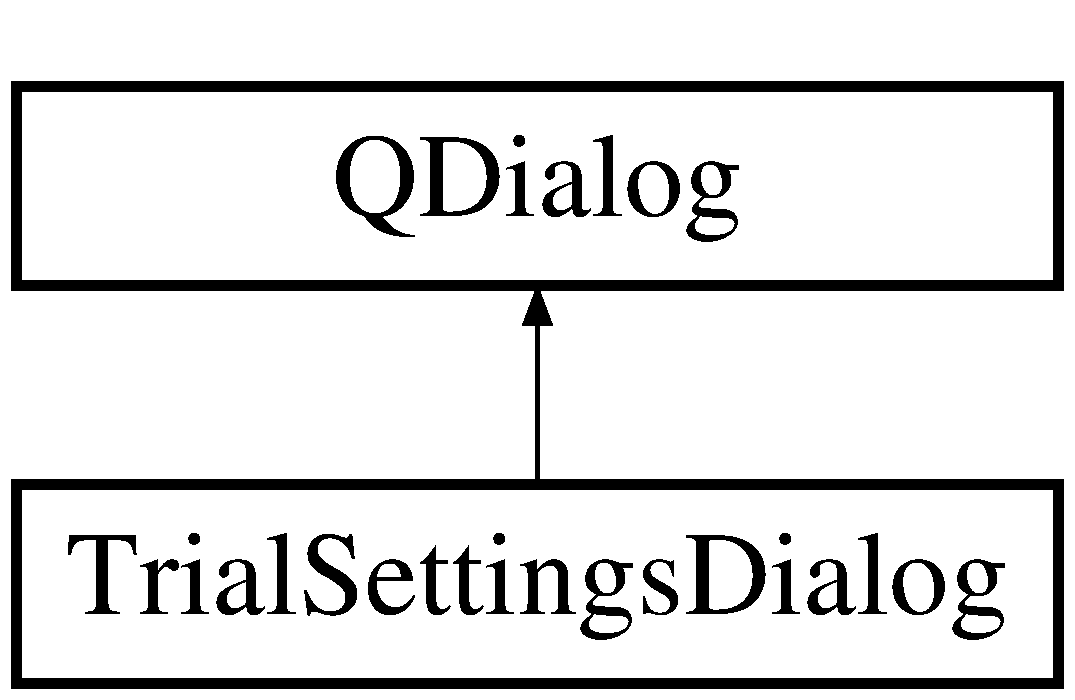
\includegraphics[height=2.000000cm]{class_trial_settings_dialog}
\end{center}
\end{figure}
\subsection*{Public Member Functions}
\begin{DoxyCompactItemize}
\item 
\hypertarget{class_trial_settings_dialog_a211e1dd92ee8e83706840e4830be96b2}{{\bfseries Trial\+Settings\+Dialog} (Q\+Widget $\ast$parent=0)}\label{class_trial_settings_dialog_a211e1dd92ee8e83706840e4830be96b2}

\item 
\hypertarget{class_trial_settings_dialog_a9dc202b2fbba3e224af466c1f1e89ea1}{Q\+String {\bfseries get\+Participant\+I\+D} ()}\label{class_trial_settings_dialog_a9dc202b2fbba3e224af466c1f1e89ea1}

\item 
\hypertarget{class_trial_settings_dialog_adc49a66cceb68c054134a99105eadf8d}{Q\+String {\bfseries get\+Age} ()}\label{class_trial_settings_dialog_adc49a66cceb68c054134a99105eadf8d}

\item 
\hypertarget{class_trial_settings_dialog_aa78d4ef979597bb258d2d1e165852996}{Q\+String {\bfseries get\+Gender} ()}\label{class_trial_settings_dialog_aa78d4ef979597bb258d2d1e165852996}

\item 
\hypertarget{class_trial_settings_dialog_aabc1f6258314e341662deb851aaf9dd6}{Q\+String {\bfseries get\+Color\+String} ()}\label{class_trial_settings_dialog_aabc1f6258314e341662deb851aaf9dd6}

\item 
\hypertarget{class_trial_settings_dialog_ade2ba0bf121c80f29bddadd6446112e4}{Q\+String {\bfseries get\+Sound\+String} ()}\label{class_trial_settings_dialog_ade2ba0bf121c80f29bddadd6446112e4}

\item 
\hypertarget{class_trial_settings_dialog_a3b3c6596fd4585606c546a32f73577fd}{Q\+String {\bfseries get\+Interface\+String} ()}\label{class_trial_settings_dialog_a3b3c6596fd4585606c546a32f73577fd}

\item 
\hypertarget{class_trial_settings_dialog_ae972a64e2b941e48a32c1bae79646e5a}{Q\+Table\+View $\ast$ {\bfseries get\+Table\+View} ()}\label{class_trial_settings_dialog_ae972a64e2b941e48a32c1bae79646e5a}

\item 
\hypertarget{class_trial_settings_dialog_a0d433b07b300b55ecf03ed224f53bb5d}{void {\bfseries set\+Participant\+I\+D} (Q\+String text)}\label{class_trial_settings_dialog_a0d433b07b300b55ecf03ed224f53bb5d}

\item 
\hypertarget{class_trial_settings_dialog_a99bb91c236188b87c235d81e15d1150b}{void {\bfseries set\+Age} (Q\+String text)}\label{class_trial_settings_dialog_a99bb91c236188b87c235d81e15d1150b}

\item 
\hypertarget{class_trial_settings_dialog_a239811adac2660a8e638addd9dc539d7}{void {\bfseries set\+Gender} (Q\+String text)}\label{class_trial_settings_dialog_a239811adac2660a8e638addd9dc539d7}

\item 
\hypertarget{class_trial_settings_dialog_a19c0c34ab166820828d0e0b2f0044ce6}{void {\bfseries set\+Color} (Q\+String text)}\label{class_trial_settings_dialog_a19c0c34ab166820828d0e0b2f0044ce6}

\item 
\hypertarget{class_trial_settings_dialog_a1658d75ea686b5a6590b4d7bf49f96af}{void {\bfseries set\+Sound} (Q\+String text)}\label{class_trial_settings_dialog_a1658d75ea686b5a6590b4d7bf49f96af}

\item 
\hypertarget{class_trial_settings_dialog_a50dec32d81641b43870111477638b0db}{void {\bfseries set\+Interface} (Q\+String text)}\label{class_trial_settings_dialog_a50dec32d81641b43870111477638b0db}

\item 
\hypertarget{class_trial_settings_dialog_a7475457608a9f46e6333953c0aef5dbd}{void {\bfseries set\+Controller} (\hyperlink{class_simon_controller}{Simon\+Controller} $\ast$controller)}\label{class_trial_settings_dialog_a7475457608a9f46e6333953c0aef5dbd}

\item 
\hypertarget{class_trial_settings_dialog_ae89add86a0324bde8f8c0b09ccea823d}{void {\bfseries close\+Event} (Q\+Close\+Event $\ast$event)}\label{class_trial_settings_dialog_ae89add86a0324bde8f8c0b09ccea823d}

\end{DoxyCompactItemize}
\subsection*{Public Attributes}
\begin{DoxyCompactItemize}
\item 
\hypertarget{class_trial_settings_dialog_a5243d4d7bcfabb3d97200339581bf434}{\hyperlink{class_trial_settings_model}{Trial\+Settings\+Model} $\ast$ {\bfseries model}}\label{class_trial_settings_dialog_a5243d4d7bcfabb3d97200339581bf434}

\item 
\hypertarget{class_trial_settings_dialog_a9c05bec82d70470481901b17df4ce07e}{int {\bfseries selected\+Row}}\label{class_trial_settings_dialog_a9c05bec82d70470481901b17df4ce07e}

\end{DoxyCompactItemize}


The documentation for this class was generated from the following files\+:\begin{DoxyCompactItemize}
\item 
U\+I/trialsettingsdialog.\+h\item 
U\+I/trialsettingsdialog.\+cpp\end{DoxyCompactItemize}

\hypertarget{class_trial_settings_model}{\section{Trial\+Settings\+Model Class Reference}
\label{class_trial_settings_model}\index{Trial\+Settings\+Model@{Trial\+Settings\+Model}}
}
\subsection*{Public Member Functions}
\begin{DoxyCompactItemize}
\item 
\hypertarget{class_trial_settings_model_a836ff2525113e876c29dab1d18d1dfee}{{\bfseries Trial\+Settings\+Model} (Q\+Table\+View $\ast$view)}\label{class_trial_settings_model_a836ff2525113e876c29dab1d18d1dfee}

\item 
void \hyperlink{class_trial_settings_model_ac6a2badb080c001eee725731918e5940}{add\+Game} (Q\+String sound, Q\+String color, Q\+String input)
\item 
void \hyperlink{class_trial_settings_model_a82883567708811acae2e0413a398ece5}{remove\+Game} (int row)
\item 
void \hyperlink{class_trial_settings_model_acf267171c19583954808dfbbf4d139e7}{start} (std\+::string pid, std\+::string ag, std\+::string gndr)
\item 
void \hyperlink{class_trial_settings_model_aaaf0d85602754b9f965ae6b248f20c89}{swap\+Rows} (int index1, int index2)
\item 
void \hyperlink{class_trial_settings_model_a2a9886471e3a978847919261010981af}{write\+Games} (std\+::string pid, std\+::string age, std\+::string gender)
\item 
void \hyperlink{class_trial_settings_model_abf028c54c71fb236ab7bdbda5ec6220a}{read\+Games} ()
\item 
void \hyperlink{class_trial_settings_model_a0f3690db59a0789e3625f9214151b3d5}{set\+Demo\+Mode} (bool md)
\item 
bool \hyperlink{class_trial_settings_model_a7de1f33a75eb321142bf561d017fe3a7}{get\+Demo\+Mode} ()
\item 
void \hyperlink{class_trial_settings_model_af7b1c0b43e04534f000f09db43baa188}{set\+Save\+Location} (std\+::string loc)
\item 
int \hyperlink{class_trial_settings_model_a48d6c2b8c99a0b177f304f1330ec96a1}{get\+Row\+Count} ()
\item 
std\+::vector$<$ std\+::string $>$ \& \hyperlink{class_trial_settings_model_ac3578447da475826046307ecbd92e0e0}{split} (const std\+::string \&s, char delim, std\+::vector$<$ std\+::string $>$ \&elems)
\item 
std\+::vector$<$ std\+::string $>$ \hyperlink{class_trial_settings_model_a283eb684102dedc1c82d36114e557481}{split} (const std\+::string \&s, char delim)
\item 
std\+::string \hyperlink{class_trial_settings_model_a02d6cb1012affee1bc4b5cc97c001268}{get\+Save\+Location} ()
\item 
Q\+String \hyperlink{class_trial_settings_model_a4da8630b29c5eedd094b5cf663890f9f}{get\+Item\+At} (int row, int col)
\end{DoxyCompactItemize}


\subsection{Member Function Documentation}
\hypertarget{class_trial_settings_model_ac6a2badb080c001eee725731918e5940}{\index{Trial\+Settings\+Model@{Trial\+Settings\+Model}!add\+Game@{add\+Game}}
\index{add\+Game@{add\+Game}!Trial\+Settings\+Model@{Trial\+Settings\+Model}}
\subsubsection[{add\+Game}]{\setlength{\rightskip}{0pt plus 5cm}void Trial\+Settings\+Model\+::add\+Game (
\begin{DoxyParamCaption}
\item[{Q\+String}]{sound, }
\item[{Q\+String}]{color, }
\item[{Q\+String}]{input}
\end{DoxyParamCaption}
)}}\label{class_trial_settings_model_ac6a2badb080c001eee725731918e5940}
Adds game to tableview and \hyperlink{class_trial_data}{Trial\+Data} \hypertarget{class_trial_settings_model_a7de1f33a75eb321142bf561d017fe3a7}{\index{Trial\+Settings\+Model@{Trial\+Settings\+Model}!get\+Demo\+Mode@{get\+Demo\+Mode}}
\index{get\+Demo\+Mode@{get\+Demo\+Mode}!Trial\+Settings\+Model@{Trial\+Settings\+Model}}
\subsubsection[{get\+Demo\+Mode}]{\setlength{\rightskip}{0pt plus 5cm}bool Trial\+Settings\+Model\+::get\+Demo\+Mode (
\begin{DoxyParamCaption}
{}
\end{DoxyParamCaption}
)}}\label{class_trial_settings_model_a7de1f33a75eb321142bf561d017fe3a7}
Getter for demo mode variable \hypertarget{class_trial_settings_model_a4da8630b29c5eedd094b5cf663890f9f}{\index{Trial\+Settings\+Model@{Trial\+Settings\+Model}!get\+Item\+At@{get\+Item\+At}}
\index{get\+Item\+At@{get\+Item\+At}!Trial\+Settings\+Model@{Trial\+Settings\+Model}}
\subsubsection[{get\+Item\+At}]{\setlength{\rightskip}{0pt plus 5cm}Q\+String Trial\+Settings\+Model\+::get\+Item\+At (
\begin{DoxyParamCaption}
\item[{int}]{row, }
\item[{int}]{col}
\end{DoxyParamCaption}
)}}\label{class_trial_settings_model_a4da8630b29c5eedd094b5cf663890f9f}
Returns the text at the specified row and column of the tableview \hypertarget{class_trial_settings_model_a48d6c2b8c99a0b177f304f1330ec96a1}{\index{Trial\+Settings\+Model@{Trial\+Settings\+Model}!get\+Row\+Count@{get\+Row\+Count}}
\index{get\+Row\+Count@{get\+Row\+Count}!Trial\+Settings\+Model@{Trial\+Settings\+Model}}
\subsubsection[{get\+Row\+Count}]{\setlength{\rightskip}{0pt plus 5cm}int Trial\+Settings\+Model\+::get\+Row\+Count (
\begin{DoxyParamCaption}
{}
\end{DoxyParamCaption}
)}}\label{class_trial_settings_model_a48d6c2b8c99a0b177f304f1330ec96a1}
Gets the number of rows in the tableview. \hypertarget{class_trial_settings_model_a02d6cb1012affee1bc4b5cc97c001268}{\index{Trial\+Settings\+Model@{Trial\+Settings\+Model}!get\+Save\+Location@{get\+Save\+Location}}
\index{get\+Save\+Location@{get\+Save\+Location}!Trial\+Settings\+Model@{Trial\+Settings\+Model}}
\subsubsection[{get\+Save\+Location}]{\setlength{\rightskip}{0pt plus 5cm}std\+::string Trial\+Settings\+Model\+::get\+Save\+Location (
\begin{DoxyParamCaption}
{}
\end{DoxyParamCaption}
)}}\label{class_trial_settings_model_a02d6cb1012affee1bc4b5cc97c001268}
Getter for save location variable \hypertarget{class_trial_settings_model_abf028c54c71fb236ab7bdbda5ec6220a}{\index{Trial\+Settings\+Model@{Trial\+Settings\+Model}!read\+Games@{read\+Games}}
\index{read\+Games@{read\+Games}!Trial\+Settings\+Model@{Trial\+Settings\+Model}}
\subsubsection[{read\+Games}]{\setlength{\rightskip}{0pt plus 5cm}void Trial\+Settings\+Model\+::read\+Games (
\begin{DoxyParamCaption}
{}
\end{DoxyParamCaption}
)}}\label{class_trial_settings_model_abf028c54c71fb236ab7bdbda5ec6220a}
Read games from config file \hypertarget{class_trial_settings_model_a82883567708811acae2e0413a398ece5}{\index{Trial\+Settings\+Model@{Trial\+Settings\+Model}!remove\+Game@{remove\+Game}}
\index{remove\+Game@{remove\+Game}!Trial\+Settings\+Model@{Trial\+Settings\+Model}}
\subsubsection[{remove\+Game}]{\setlength{\rightskip}{0pt plus 5cm}void Trial\+Settings\+Model\+::remove\+Game (
\begin{DoxyParamCaption}
\item[{int}]{row}
\end{DoxyParamCaption}
)}}\label{class_trial_settings_model_a82883567708811acae2e0413a398ece5}
Deletes a row from the table. \hypertarget{class_trial_settings_model_a0f3690db59a0789e3625f9214151b3d5}{\index{Trial\+Settings\+Model@{Trial\+Settings\+Model}!set\+Demo\+Mode@{set\+Demo\+Mode}}
\index{set\+Demo\+Mode@{set\+Demo\+Mode}!Trial\+Settings\+Model@{Trial\+Settings\+Model}}
\subsubsection[{set\+Demo\+Mode}]{\setlength{\rightskip}{0pt plus 5cm}void Trial\+Settings\+Model\+::set\+Demo\+Mode (
\begin{DoxyParamCaption}
\item[{bool}]{md}
\end{DoxyParamCaption}
)}}\label{class_trial_settings_model_a0f3690db59a0789e3625f9214151b3d5}
Setter for private demomode variable \hypertarget{class_trial_settings_model_af7b1c0b43e04534f000f09db43baa188}{\index{Trial\+Settings\+Model@{Trial\+Settings\+Model}!set\+Save\+Location@{set\+Save\+Location}}
\index{set\+Save\+Location@{set\+Save\+Location}!Trial\+Settings\+Model@{Trial\+Settings\+Model}}
\subsubsection[{set\+Save\+Location}]{\setlength{\rightskip}{0pt plus 5cm}void Trial\+Settings\+Model\+::set\+Save\+Location (
\begin{DoxyParamCaption}
\item[{std\+::string}]{loc}
\end{DoxyParamCaption}
)}}\label{class_trial_settings_model_af7b1c0b43e04534f000f09db43baa188}
Sets the C\+S\+V save location \hypertarget{class_trial_settings_model_ac3578447da475826046307ecbd92e0e0}{\index{Trial\+Settings\+Model@{Trial\+Settings\+Model}!split@{split}}
\index{split@{split}!Trial\+Settings\+Model@{Trial\+Settings\+Model}}
\subsubsection[{split}]{\setlength{\rightskip}{0pt plus 5cm}std\+::vector$<$ std\+::string $>$ \& Trial\+Settings\+Model\+::split (
\begin{DoxyParamCaption}
\item[{const std\+::string \&}]{s, }
\item[{char}]{delim, }
\item[{std\+::vector$<$ std\+::string $>$ \&}]{elems}
\end{DoxyParamCaption}
)}}\label{class_trial_settings_model_ac3578447da475826046307ecbd92e0e0}
Split helper function \hypertarget{class_trial_settings_model_a283eb684102dedc1c82d36114e557481}{\index{Trial\+Settings\+Model@{Trial\+Settings\+Model}!split@{split}}
\index{split@{split}!Trial\+Settings\+Model@{Trial\+Settings\+Model}}
\subsubsection[{split}]{\setlength{\rightskip}{0pt plus 5cm}std\+::vector$<$ std\+::string $>$ Trial\+Settings\+Model\+::split (
\begin{DoxyParamCaption}
\item[{const std\+::string \&}]{s, }
\item[{char}]{delim}
\end{DoxyParamCaption}
)}}\label{class_trial_settings_model_a283eb684102dedc1c82d36114e557481}
The same as Java String.\+split \hypertarget{class_trial_settings_model_acf267171c19583954808dfbbf4d139e7}{\index{Trial\+Settings\+Model@{Trial\+Settings\+Model}!start@{start}}
\index{start@{start}!Trial\+Settings\+Model@{Trial\+Settings\+Model}}
\subsubsection[{start}]{\setlength{\rightskip}{0pt plus 5cm}void Trial\+Settings\+Model\+::start (
\begin{DoxyParamCaption}
\item[{std\+::string}]{pid, }
\item[{std\+::string}]{ag, }
\item[{std\+::string}]{gndr}
\end{DoxyParamCaption}
)}}\label{class_trial_settings_model_acf267171c19583954808dfbbf4d139e7}
Start running the Simon game \hypertarget{class_trial_settings_model_aaaf0d85602754b9f965ae6b248f20c89}{\index{Trial\+Settings\+Model@{Trial\+Settings\+Model}!swap\+Rows@{swap\+Rows}}
\index{swap\+Rows@{swap\+Rows}!Trial\+Settings\+Model@{Trial\+Settings\+Model}}
\subsubsection[{swap\+Rows}]{\setlength{\rightskip}{0pt plus 5cm}void Trial\+Settings\+Model\+::swap\+Rows (
\begin{DoxyParamCaption}
\item[{int}]{index1, }
\item[{int}]{index2}
\end{DoxyParamCaption}
)}}\label{class_trial_settings_model_aaaf0d85602754b9f965ae6b248f20c89}
Swap two rows in the table. Used for moves and such. \hypertarget{class_trial_settings_model_a2a9886471e3a978847919261010981af}{\index{Trial\+Settings\+Model@{Trial\+Settings\+Model}!write\+Games@{write\+Games}}
\index{write\+Games@{write\+Games}!Trial\+Settings\+Model@{Trial\+Settings\+Model}}
\subsubsection[{write\+Games}]{\setlength{\rightskip}{0pt plus 5cm}void Trial\+Settings\+Model\+::write\+Games (
\begin{DoxyParamCaption}
\item[{std\+::string}]{pid, }
\item[{std\+::string}]{age, }
\item[{std\+::string}]{gender}
\end{DoxyParamCaption}
)}}\label{class_trial_settings_model_a2a9886471e3a978847919261010981af}
Write game to config file 

The documentation for this class was generated from the following files\+:\begin{DoxyCompactItemize}
\item 
U\+I/trialsettingsmodel.\+h\item 
U\+I/trialsettingsmodel.\+cpp\end{DoxyCompactItemize}

\hypertarget{struct_leap_1_1_vector}{\section{Leap\+:\+:Vector Struct Reference}
\label{struct_leap_1_1_vector}\index{Leap\+::\+Vector@{Leap\+::\+Vector}}
}


{\ttfamily \#include $<$Leap\+Math.\+h$>$}

\subsection*{Public Member Functions}
\begin{DoxyCompactItemize}
\item 
\hyperlink{struct_leap_1_1_vector_a0d7a6417136be2cde1ddd56c39244929}{Vector} ()
\item 
\hyperlink{struct_leap_1_1_vector_a58bde18133811a15d122a785f0b36b80}{Vector} (float \+\_\+x, float \+\_\+y, float \+\_\+z)
\item 
\hyperlink{struct_leap_1_1_vector_a2b271c5d88e466f17771e62bd8faea94}{Vector} (const \hyperlink{struct_leap_1_1_vector}{Vector} \&vector)
\item 
float \hyperlink{struct_leap_1_1_vector_ab7955521f3b80e2b2ad9b67330345476}{magnitude} () const 
\item 
float \hyperlink{struct_leap_1_1_vector_a81226e9b68a8ee06124237145d16b77c}{magnitude\+Squared} () const 
\item 
float \hyperlink{struct_leap_1_1_vector_adfda206e0659c44a2eb632bc2a8cd82a}{distance\+To} (const \hyperlink{struct_leap_1_1_vector}{Vector} \&other) const 
\item 
float \hyperlink{struct_leap_1_1_vector_ac8db3180325f86971f1089ef17808c24}{angle\+To} (const \hyperlink{struct_leap_1_1_vector}{Vector} \&other) const 
\item 
float \hyperlink{struct_leap_1_1_vector_a206cee5e82cc8f860edae69c4f101a49}{pitch} () const 
\item 
float \hyperlink{struct_leap_1_1_vector_aa4bdfa69695be1e5a6db629685538239}{yaw} () const 
\item 
float \hyperlink{struct_leap_1_1_vector_a11dc02be2e993142ac422b7b3a7428c1}{roll} () const 
\item 
float \hyperlink{struct_leap_1_1_vector_a80f93cc43a55259acd366ecefcb3766a}{dot} (const \hyperlink{struct_leap_1_1_vector}{Vector} \&other) const 
\item 
\hyperlink{struct_leap_1_1_vector}{Vector} \hyperlink{struct_leap_1_1_vector_ad67607a021ae7e8913efea37aac55087}{cross} (const \hyperlink{struct_leap_1_1_vector}{Vector} \&other) const 
\item 
\hyperlink{struct_leap_1_1_vector}{Vector} \hyperlink{struct_leap_1_1_vector_a23d7640c4797fb84367272d4ebd88e8a}{normalized} () const 
\item 
\hyperlink{struct_leap_1_1_vector}{Vector} \hyperlink{struct_leap_1_1_vector_a05564e30c0301990e6f5ecea81fc0f4a}{operator-\/} () const 
\item 
\hyperlink{struct_leap_1_1_vector}{Vector} \hyperlink{struct_leap_1_1_vector_ae5f8d3473a15cff36a610e3f339c7423}{operator+} (const \hyperlink{struct_leap_1_1_vector}{Vector} \&other) const 
\item 
\hyperlink{struct_leap_1_1_vector}{Vector} \hyperlink{struct_leap_1_1_vector_a4a729e5a27fe13d3c71a7a9fd3e234e3}{operator-\/} (const \hyperlink{struct_leap_1_1_vector}{Vector} \&other) const 
\item 
\hyperlink{struct_leap_1_1_vector}{Vector} \hyperlink{struct_leap_1_1_vector_adfac06b2c9a9936f62da4b293ef98db3}{operator$\ast$} (float scalar) const 
\item 
\hyperlink{struct_leap_1_1_vector}{Vector} \hyperlink{struct_leap_1_1_vector_a23a7ee5a8da0f282e51628ac3fc59f70}{operator/} (float scalar) const 
\item 
\hyperlink{struct_leap_1_1_vector}{Vector} \& \hyperlink{struct_leap_1_1_vector_ac2dbd10e09399bc5679ceee380cff2cc}{operator+=} (const \hyperlink{struct_leap_1_1_vector}{Vector} \&other)
\item 
\hyperlink{struct_leap_1_1_vector}{Vector} \& \hyperlink{struct_leap_1_1_vector_a71f56cf12c752f001d44c6a9ed3c15db}{operator-\/=} (const \hyperlink{struct_leap_1_1_vector}{Vector} \&other)
\item 
\hyperlink{struct_leap_1_1_vector}{Vector} \& \hyperlink{struct_leap_1_1_vector_a3c07a9eb80762ca448a78650500f06a8}{operator$\ast$=} (float scalar)
\item 
\hyperlink{struct_leap_1_1_vector}{Vector} \& \hyperlink{struct_leap_1_1_vector_a0c83e9d07018bdb3b3404088939a050d}{operator/=} (float scalar)
\item 
std\+::string \hyperlink{struct_leap_1_1_vector_a06f42a3c10c886b449e6db32a565099c}{to\+String} () const 
\item 
bool \hyperlink{struct_leap_1_1_vector_a3055b0255b5d4af0a51ceacd93187218}{operator==} (const \hyperlink{struct_leap_1_1_vector}{Vector} \&other) const 
\item 
bool \hyperlink{struct_leap_1_1_vector_abf6930c4b2ed673408d86194626577b0}{operator!=} (const \hyperlink{struct_leap_1_1_vector}{Vector} \&other) const 
\item 
bool \hyperlink{struct_leap_1_1_vector_ae8f445cd11ba6bd4a45de05551277a45}{is\+Valid} () const 
\item 
float \hyperlink{struct_leap_1_1_vector_a45db0a2e00a86c1b9bf7e68ae6b9a20e}{operator\mbox{[}$\,$\mbox{]}} (unsigned int index) const 
\item 
const float $\ast$ \hyperlink{struct_leap_1_1_vector_ad41fdd88c7097efb13b3cb34e2752777}{to\+Float\+Pointer} () const 
\item 
{\footnotesize template$<$typename Vector3\+Type $>$ }\\const Vector3\+Type \hyperlink{struct_leap_1_1_vector_a55fc5ddc43e74988d48797d31a0849f4}{to\+Vector3} () const 
\item 
{\footnotesize template$<$typename Vector4\+Type $>$ }\\const Vector4\+Type \hyperlink{struct_leap_1_1_vector_a2adaf93670f1069e40532d39eb974b3f}{to\+Vector4} (float w=0.\+0f) const 
\end{DoxyCompactItemize}
\subsection*{Static Public Member Functions}
\begin{DoxyCompactItemize}
\item 
static const \hyperlink{struct_leap_1_1_vector}{Vector} \& \hyperlink{struct_leap_1_1_vector_a743b469003fa6622a00ff277d2481da9}{zero} ()
\item 
static const \hyperlink{struct_leap_1_1_vector}{Vector} \& \hyperlink{struct_leap_1_1_vector_a0d90c96672e7ee90fb510d7b96c32861}{x\+Axis} ()
\item 
static const \hyperlink{struct_leap_1_1_vector}{Vector} \& \hyperlink{struct_leap_1_1_vector_a9a387eb8ab05e55708542c031c641f31}{y\+Axis} ()
\item 
static const \hyperlink{struct_leap_1_1_vector}{Vector} \& \hyperlink{struct_leap_1_1_vector_a6ec3652d02a9599bc2a00411a1e05501}{z\+Axis} ()
\item 
static const \hyperlink{struct_leap_1_1_vector}{Vector} \& \hyperlink{struct_leap_1_1_vector_a315ffbbd7f686e1d93bffc6beb11f89d}{left} ()
\item 
static const \hyperlink{struct_leap_1_1_vector}{Vector} \& \hyperlink{struct_leap_1_1_vector_aa4d509a1640d9aa270d095c9ae8e44f2}{right} ()
\item 
static const \hyperlink{struct_leap_1_1_vector}{Vector} \& \hyperlink{struct_leap_1_1_vector_ac1c62a2d280d7a7c67e99f1996076b58}{down} ()
\item 
static const \hyperlink{struct_leap_1_1_vector}{Vector} \& \hyperlink{struct_leap_1_1_vector_a0a38a683c0224b38b75d58db24f51adf}{up} ()
\item 
static const \hyperlink{struct_leap_1_1_vector}{Vector} \& \hyperlink{struct_leap_1_1_vector_a79b32a38e4c99b6ddbf94ac22680d405}{forward} ()
\item 
static const \hyperlink{struct_leap_1_1_vector}{Vector} \& \hyperlink{struct_leap_1_1_vector_a82ea3abc8ae6bb144a5946836fce88ad}{backward} ()
\end{DoxyCompactItemize}
\subsection*{Public Attributes}
\begin{DoxyCompactItemize}
\item 
float \hyperlink{struct_leap_1_1_vector_a58ab75fe089da2070f5dcef82c9a578a}{x}
\item 
float \hyperlink{struct_leap_1_1_vector_abfff2f5b5c10d58a43cf377fc4cb9951}{y}
\item 
float \hyperlink{struct_leap_1_1_vector_aa44971ce01ce035e78ea557bc1e983a4}{z}
\end{DoxyCompactItemize}
\subsection*{Friends}
\begin{DoxyCompactItemize}
\item 
\hyperlink{struct_leap_1_1_vector}{Vector} \hyperlink{struct_leap_1_1_vector_a90f989718db5a1be59eb472f30e61472}{operator$\ast$} (float scalar, const \hyperlink{struct_leap_1_1_vector}{Vector} \&vector)
\item 
std\+::ostream \& \hyperlink{struct_leap_1_1_vector_ae295e87eb813266c27e75d2809df2acc}{operator$<$$<$} (std\+::ostream \&out, const \hyperlink{struct_leap_1_1_vector}{Vector} \&vector)
\end{DoxyCompactItemize}


\subsection{Detailed Description}
The \hyperlink{struct_leap_1_1_vector}{Vector} struct represents a three-\/component mathematical vector or point such as a direction or position in three-\/dimensional space.

The Leap Motion software employs a right-\/handed Cartesian coordinate system. Values given are in units of real-\/world millimeters. The origin is centered at the center of the Leap Motion \hyperlink{class_leap_1_1_controller}{Controller}. The x-\/ and z-\/axes lie in the horizontal plane, with the x-\/axis running parallel to the long edge of the device. The y-\/axis is vertical, with positive values increasing upwards (in contrast to the downward orientation of most computer graphics coordinate systems). The z-\/axis has positive values increasing away from the computer screen.

 \begin{DoxySince}{Since}
1.\+0 
\end{DoxySince}


\subsection{Constructor \& Destructor Documentation}
\hypertarget{struct_leap_1_1_vector_a0d7a6417136be2cde1ddd56c39244929}{\index{Leap\+::\+Vector@{Leap\+::\+Vector}!Vector@{Vector}}
\index{Vector@{Vector}!Leap\+::\+Vector@{Leap\+::\+Vector}}
\subsubsection[{Vector}]{\setlength{\rightskip}{0pt plus 5cm}Leap\+::\+Vector\+::\+Vector (
\begin{DoxyParamCaption}
{}
\end{DoxyParamCaption}
)\hspace{0.3cm}{\ttfamily [inline]}}}\label{struct_leap_1_1_vector_a0d7a6417136be2cde1ddd56c39244929}
Creates a new \hyperlink{struct_leap_1_1_vector}{Vector} with all components set to zero. \begin{DoxySince}{Since}
1.\+0 
\end{DoxySince}
\hypertarget{struct_leap_1_1_vector_a58bde18133811a15d122a785f0b36b80}{\index{Leap\+::\+Vector@{Leap\+::\+Vector}!Vector@{Vector}}
\index{Vector@{Vector}!Leap\+::\+Vector@{Leap\+::\+Vector}}
\subsubsection[{Vector}]{\setlength{\rightskip}{0pt plus 5cm}Leap\+::\+Vector\+::\+Vector (
\begin{DoxyParamCaption}
\item[{float}]{\+\_\+x, }
\item[{float}]{\+\_\+y, }
\item[{float}]{\+\_\+z}
\end{DoxyParamCaption}
)\hspace{0.3cm}{\ttfamily [inline]}}}\label{struct_leap_1_1_vector_a58bde18133811a15d122a785f0b36b80}
Creates a new \hyperlink{struct_leap_1_1_vector}{Vector} with the specified component values.


\begin{DoxyCodeInclude}
\end{DoxyCodeInclude}
 \begin{DoxySince}{Since}
1.\+0 
\end{DoxySince}
\hypertarget{struct_leap_1_1_vector_a2b271c5d88e466f17771e62bd8faea94}{\index{Leap\+::\+Vector@{Leap\+::\+Vector}!Vector@{Vector}}
\index{Vector@{Vector}!Leap\+::\+Vector@{Leap\+::\+Vector}}
\subsubsection[{Vector}]{\setlength{\rightskip}{0pt plus 5cm}Leap\+::\+Vector\+::\+Vector (
\begin{DoxyParamCaption}
\item[{const {\bf Vector} \&}]{vector}
\end{DoxyParamCaption}
)\hspace{0.3cm}{\ttfamily [inline]}}}\label{struct_leap_1_1_vector_a2b271c5d88e466f17771e62bd8faea94}
Copies the specified \hyperlink{struct_leap_1_1_vector}{Vector}.


\begin{DoxyCodeInclude}
\end{DoxyCodeInclude}
 \begin{DoxySince}{Since}
1.\+0 
\end{DoxySince}


\subsection{Member Function Documentation}
\hypertarget{struct_leap_1_1_vector_ac8db3180325f86971f1089ef17808c24}{\index{Leap\+::\+Vector@{Leap\+::\+Vector}!angle\+To@{angle\+To}}
\index{angle\+To@{angle\+To}!Leap\+::\+Vector@{Leap\+::\+Vector}}
\subsubsection[{angle\+To}]{\setlength{\rightskip}{0pt plus 5cm}float Leap\+::\+Vector\+::angle\+To (
\begin{DoxyParamCaption}
\item[{const {\bf Vector} \&}]{other}
\end{DoxyParamCaption}
) const\hspace{0.3cm}{\ttfamily [inline]}}}\label{struct_leap_1_1_vector_ac8db3180325f86971f1089ef17808c24}
The angle between this vector and the specified vector in radians.

The angle is measured in the plane formed by the two vectors. The angle returned is always the smaller of the two conjugate angles. Thus {\ttfamily A.\+angle\+To(\+B) == B.\+angle\+To(\+A)} and is always a positive value less than or equal to pi radians (180 degrees).

If either vector has zero length, then this function returns zero.




\begin{DoxyCodeInclude}
\end{DoxyCodeInclude}



\begin{DoxyParams}{Parameters}
{\em other} & A \hyperlink{struct_leap_1_1_vector}{Vector} object. \\
\hline
\end{DoxyParams}
\begin{DoxyReturn}{Returns}
The angle between this vector and the specified vector in radians. 
\end{DoxyReturn}
\begin{DoxySince}{Since}
1.\+0 
\end{DoxySince}
\hypertarget{struct_leap_1_1_vector_a82ea3abc8ae6bb144a5946836fce88ad}{\index{Leap\+::\+Vector@{Leap\+::\+Vector}!backward@{backward}}
\index{backward@{backward}!Leap\+::\+Vector@{Leap\+::\+Vector}}
\subsubsection[{backward}]{\setlength{\rightskip}{0pt plus 5cm}static const {\bf Vector}\& Leap\+::\+Vector\+::backward (
\begin{DoxyParamCaption}
{}
\end{DoxyParamCaption}
)\hspace{0.3cm}{\ttfamily [inline]}, {\ttfamily [static]}}}\label{struct_leap_1_1_vector_a82ea3abc8ae6bb144a5946836fce88ad}
The unit vector pointing backward along the positive z-\/axis\+: (0, 0, 1)


\begin{DoxyCodeInclude}
\end{DoxyCodeInclude}
 \begin{DoxySince}{Since}
1.\+0 
\end{DoxySince}
\hypertarget{struct_leap_1_1_vector_ad67607a021ae7e8913efea37aac55087}{\index{Leap\+::\+Vector@{Leap\+::\+Vector}!cross@{cross}}
\index{cross@{cross}!Leap\+::\+Vector@{Leap\+::\+Vector}}
\subsubsection[{cross}]{\setlength{\rightskip}{0pt plus 5cm}{\bf Vector} Leap\+::\+Vector\+::cross (
\begin{DoxyParamCaption}
\item[{const {\bf Vector} \&}]{other}
\end{DoxyParamCaption}
) const\hspace{0.3cm}{\ttfamily [inline]}}}\label{struct_leap_1_1_vector_ad67607a021ae7e8913efea37aac55087}
The cross product of this vector and the specified vector.

The cross product is a vector orthogonal to both original vectors. It has a magnitude equal to the area of a parallelogram having the two vectors as sides. The direction of the returned vector is determined by the right-\/hand rule. Thus {\ttfamily A.\+cross(\+B) == -\/\+B.\+cross(A).}




\begin{DoxyCodeInclude}
\end{DoxyCodeInclude}



\begin{DoxyParams}{Parameters}
{\em other} & A \hyperlink{struct_leap_1_1_vector}{Vector} object. \\
\hline
\end{DoxyParams}
\begin{DoxyReturn}{Returns}
The cross product of this vector and the specified vector. 
\end{DoxyReturn}
\begin{DoxySince}{Since}
1.\+0 
\end{DoxySince}
\hypertarget{struct_leap_1_1_vector_adfda206e0659c44a2eb632bc2a8cd82a}{\index{Leap\+::\+Vector@{Leap\+::\+Vector}!distance\+To@{distance\+To}}
\index{distance\+To@{distance\+To}!Leap\+::\+Vector@{Leap\+::\+Vector}}
\subsubsection[{distance\+To}]{\setlength{\rightskip}{0pt plus 5cm}float Leap\+::\+Vector\+::distance\+To (
\begin{DoxyParamCaption}
\item[{const {\bf Vector} \&}]{other}
\end{DoxyParamCaption}
) const\hspace{0.3cm}{\ttfamily [inline]}}}\label{struct_leap_1_1_vector_adfda206e0659c44a2eb632bc2a8cd82a}
The distance between the point represented by this \hyperlink{struct_leap_1_1_vector}{Vector} object and a point represented by the specified \hyperlink{struct_leap_1_1_vector}{Vector} object.


\begin{DoxyCodeInclude}
\end{DoxyCodeInclude}



\begin{DoxyParams}{Parameters}
{\em other} & A \hyperlink{struct_leap_1_1_vector}{Vector} object. \\
\hline
\end{DoxyParams}
\begin{DoxyReturn}{Returns}
The distance from this point to the specified point. 
\end{DoxyReturn}
\begin{DoxySince}{Since}
1.\+0 
\end{DoxySince}
\hypertarget{struct_leap_1_1_vector_a80f93cc43a55259acd366ecefcb3766a}{\index{Leap\+::\+Vector@{Leap\+::\+Vector}!dot@{dot}}
\index{dot@{dot}!Leap\+::\+Vector@{Leap\+::\+Vector}}
\subsubsection[{dot}]{\setlength{\rightskip}{0pt plus 5cm}float Leap\+::\+Vector\+::dot (
\begin{DoxyParamCaption}
\item[{const {\bf Vector} \&}]{other}
\end{DoxyParamCaption}
) const\hspace{0.3cm}{\ttfamily [inline]}}}\label{struct_leap_1_1_vector_a80f93cc43a55259acd366ecefcb3766a}
The dot product of this vector with another vector.

The dot product is the magnitude of the projection of this vector onto the specified vector.




\begin{DoxyCodeInclude}
\end{DoxyCodeInclude}



\begin{DoxyParams}{Parameters}
{\em other} & A \hyperlink{struct_leap_1_1_vector}{Vector} object. \\
\hline
\end{DoxyParams}
\begin{DoxyReturn}{Returns}
The dot product of this vector and the specified vector. 
\end{DoxyReturn}
\begin{DoxySince}{Since}
1.\+0 
\end{DoxySince}
\hypertarget{struct_leap_1_1_vector_ac1c62a2d280d7a7c67e99f1996076b58}{\index{Leap\+::\+Vector@{Leap\+::\+Vector}!down@{down}}
\index{down@{down}!Leap\+::\+Vector@{Leap\+::\+Vector}}
\subsubsection[{down}]{\setlength{\rightskip}{0pt plus 5cm}static const {\bf Vector}\& Leap\+::\+Vector\+::down (
\begin{DoxyParamCaption}
{}
\end{DoxyParamCaption}
)\hspace{0.3cm}{\ttfamily [inline]}, {\ttfamily [static]}}}\label{struct_leap_1_1_vector_ac1c62a2d280d7a7c67e99f1996076b58}
The unit vector pointing down along the negative y-\/axis\+: (0, -\/1, 0)


\begin{DoxyCodeInclude}
\end{DoxyCodeInclude}
 \begin{DoxySince}{Since}
1.\+0 
\end{DoxySince}
\hypertarget{struct_leap_1_1_vector_a79b32a38e4c99b6ddbf94ac22680d405}{\index{Leap\+::\+Vector@{Leap\+::\+Vector}!forward@{forward}}
\index{forward@{forward}!Leap\+::\+Vector@{Leap\+::\+Vector}}
\subsubsection[{forward}]{\setlength{\rightskip}{0pt plus 5cm}static const {\bf Vector}\& Leap\+::\+Vector\+::forward (
\begin{DoxyParamCaption}
{}
\end{DoxyParamCaption}
)\hspace{0.3cm}{\ttfamily [inline]}, {\ttfamily [static]}}}\label{struct_leap_1_1_vector_a79b32a38e4c99b6ddbf94ac22680d405}
The unit vector pointing forward along the negative z-\/axis\+: (0, 0, -\/1)


\begin{DoxyCodeInclude}
\end{DoxyCodeInclude}
 \begin{DoxySince}{Since}
1.\+0 
\end{DoxySince}
\hypertarget{struct_leap_1_1_vector_ae8f445cd11ba6bd4a45de05551277a45}{\index{Leap\+::\+Vector@{Leap\+::\+Vector}!is\+Valid@{is\+Valid}}
\index{is\+Valid@{is\+Valid}!Leap\+::\+Vector@{Leap\+::\+Vector}}
\subsubsection[{is\+Valid}]{\setlength{\rightskip}{0pt plus 5cm}bool Leap\+::\+Vector\+::is\+Valid (
\begin{DoxyParamCaption}
{}
\end{DoxyParamCaption}
) const\hspace{0.3cm}{\ttfamily [inline]}}}\label{struct_leap_1_1_vector_ae8f445cd11ba6bd4a45de05551277a45}
Returns true if all of the vector's components are finite. If any component is Na\+N or infinite, then this returns false.


\begin{DoxyCodeInclude}
\end{DoxyCodeInclude}
 \begin{DoxySince}{Since}
1.\+0 
\end{DoxySince}
\hypertarget{struct_leap_1_1_vector_a315ffbbd7f686e1d93bffc6beb11f89d}{\index{Leap\+::\+Vector@{Leap\+::\+Vector}!left@{left}}
\index{left@{left}!Leap\+::\+Vector@{Leap\+::\+Vector}}
\subsubsection[{left}]{\setlength{\rightskip}{0pt plus 5cm}static const {\bf Vector}\& Leap\+::\+Vector\+::left (
\begin{DoxyParamCaption}
{}
\end{DoxyParamCaption}
)\hspace{0.3cm}{\ttfamily [inline]}, {\ttfamily [static]}}}\label{struct_leap_1_1_vector_a315ffbbd7f686e1d93bffc6beb11f89d}
The unit vector pointing left along the negative x-\/axis\+: (-\/1, 0, 0)


\begin{DoxyCodeInclude}
\end{DoxyCodeInclude}
 \begin{DoxySince}{Since}
1.\+0 
\end{DoxySince}
\hypertarget{struct_leap_1_1_vector_ab7955521f3b80e2b2ad9b67330345476}{\index{Leap\+::\+Vector@{Leap\+::\+Vector}!magnitude@{magnitude}}
\index{magnitude@{magnitude}!Leap\+::\+Vector@{Leap\+::\+Vector}}
\subsubsection[{magnitude}]{\setlength{\rightskip}{0pt plus 5cm}float Leap\+::\+Vector\+::magnitude (
\begin{DoxyParamCaption}
{}
\end{DoxyParamCaption}
) const\hspace{0.3cm}{\ttfamily [inline]}}}\label{struct_leap_1_1_vector_ab7955521f3b80e2b2ad9b67330345476}
The magnitude, or length, of this vector.

The magnitude is the L2 norm, or Euclidean distance between the origin and the point represented by the (x, y, z) components of this \hyperlink{struct_leap_1_1_vector}{Vector} object.


\begin{DoxyCodeInclude}
\end{DoxyCodeInclude}


\begin{DoxyReturn}{Returns}
The length of this vector. 
\end{DoxyReturn}
\begin{DoxySince}{Since}
1.\+0 
\end{DoxySince}
\hypertarget{struct_leap_1_1_vector_a81226e9b68a8ee06124237145d16b77c}{\index{Leap\+::\+Vector@{Leap\+::\+Vector}!magnitude\+Squared@{magnitude\+Squared}}
\index{magnitude\+Squared@{magnitude\+Squared}!Leap\+::\+Vector@{Leap\+::\+Vector}}
\subsubsection[{magnitude\+Squared}]{\setlength{\rightskip}{0pt plus 5cm}float Leap\+::\+Vector\+::magnitude\+Squared (
\begin{DoxyParamCaption}
{}
\end{DoxyParamCaption}
) const\hspace{0.3cm}{\ttfamily [inline]}}}\label{struct_leap_1_1_vector_a81226e9b68a8ee06124237145d16b77c}
The square of the magnitude, or length, of this vector.


\begin{DoxyCodeInclude}
\end{DoxyCodeInclude}


\begin{DoxyReturn}{Returns}
The square of the length of this vector. 
\end{DoxyReturn}
\begin{DoxySince}{Since}
1.\+0 
\end{DoxySince}
\hypertarget{struct_leap_1_1_vector_a23d7640c4797fb84367272d4ebd88e8a}{\index{Leap\+::\+Vector@{Leap\+::\+Vector}!normalized@{normalized}}
\index{normalized@{normalized}!Leap\+::\+Vector@{Leap\+::\+Vector}}
\subsubsection[{normalized}]{\setlength{\rightskip}{0pt plus 5cm}{\bf Vector} Leap\+::\+Vector\+::normalized (
\begin{DoxyParamCaption}
{}
\end{DoxyParamCaption}
) const\hspace{0.3cm}{\ttfamily [inline]}}}\label{struct_leap_1_1_vector_a23d7640c4797fb84367272d4ebd88e8a}
A normalized copy of this vector.

A normalized vector has the same direction as the original vector, but with a length of one.


\begin{DoxyCodeInclude}
\end{DoxyCodeInclude}


\begin{DoxyReturn}{Returns}
A \hyperlink{struct_leap_1_1_vector}{Vector} object with a length of one, pointing in the same direction as this \hyperlink{struct_leap_1_1_vector}{Vector} object. 
\end{DoxyReturn}
\begin{DoxySince}{Since}
1.\+0 
\end{DoxySince}
\hypertarget{struct_leap_1_1_vector_abf6930c4b2ed673408d86194626577b0}{\index{Leap\+::\+Vector@{Leap\+::\+Vector}!operator"!=@{operator"!=}}
\index{operator"!=@{operator"!=}!Leap\+::\+Vector@{Leap\+::\+Vector}}
\subsubsection[{operator"!=}]{\setlength{\rightskip}{0pt plus 5cm}bool Leap\+::\+Vector\+::operator!= (
\begin{DoxyParamCaption}
\item[{const {\bf Vector} \&}]{other}
\end{DoxyParamCaption}
) const\hspace{0.3cm}{\ttfamily [inline]}}}\label{struct_leap_1_1_vector_abf6930c4b2ed673408d86194626577b0}
Compare \hyperlink{struct_leap_1_1_vector}{Vector} inequality component-\/wise.


\begin{DoxyCodeInclude}
\end{DoxyCodeInclude}
 \begin{DoxySince}{Since}
1.\+0 
\end{DoxySince}
\hypertarget{struct_leap_1_1_vector_adfac06b2c9a9936f62da4b293ef98db3}{\index{Leap\+::\+Vector@{Leap\+::\+Vector}!operator$\ast$@{operator$\ast$}}
\index{operator$\ast$@{operator$\ast$}!Leap\+::\+Vector@{Leap\+::\+Vector}}
\subsubsection[{operator$\ast$}]{\setlength{\rightskip}{0pt plus 5cm}{\bf Vector} Leap\+::\+Vector\+::operator$\ast$ (
\begin{DoxyParamCaption}
\item[{float}]{scalar}
\end{DoxyParamCaption}
) const\hspace{0.3cm}{\ttfamily [inline]}}}\label{struct_leap_1_1_vector_adfac06b2c9a9936f62da4b293ef98db3}
Multiply vector by a scalar.


\begin{DoxyCodeInclude}
\end{DoxyCodeInclude}
 \begin{DoxySince}{Since}
1.\+0 
\end{DoxySince}
\hypertarget{struct_leap_1_1_vector_a3c07a9eb80762ca448a78650500f06a8}{\index{Leap\+::\+Vector@{Leap\+::\+Vector}!operator$\ast$=@{operator$\ast$=}}
\index{operator$\ast$=@{operator$\ast$=}!Leap\+::\+Vector@{Leap\+::\+Vector}}
\subsubsection[{operator$\ast$=}]{\setlength{\rightskip}{0pt plus 5cm}{\bf Vector}\& Leap\+::\+Vector\+::operator$\ast$= (
\begin{DoxyParamCaption}
\item[{float}]{scalar}
\end{DoxyParamCaption}
)\hspace{0.3cm}{\ttfamily [inline]}}}\label{struct_leap_1_1_vector_a3c07a9eb80762ca448a78650500f06a8}
Multiply vector by a scalar and assign the product. \begin{DoxySince}{Since}
1.\+0 
\end{DoxySince}
\hypertarget{struct_leap_1_1_vector_ae5f8d3473a15cff36a610e3f339c7423}{\index{Leap\+::\+Vector@{Leap\+::\+Vector}!operator+@{operator+}}
\index{operator+@{operator+}!Leap\+::\+Vector@{Leap\+::\+Vector}}
\subsubsection[{operator+}]{\setlength{\rightskip}{0pt plus 5cm}{\bf Vector} Leap\+::\+Vector\+::operator+ (
\begin{DoxyParamCaption}
\item[{const {\bf Vector} \&}]{other}
\end{DoxyParamCaption}
) const\hspace{0.3cm}{\ttfamily [inline]}}}\label{struct_leap_1_1_vector_ae5f8d3473a15cff36a610e3f339c7423}
Add vectors component-\/wise.


\begin{DoxyCodeInclude}
\end{DoxyCodeInclude}
 \begin{DoxySince}{Since}
1.\+0 
\end{DoxySince}
\hypertarget{struct_leap_1_1_vector_ac2dbd10e09399bc5679ceee380cff2cc}{\index{Leap\+::\+Vector@{Leap\+::\+Vector}!operator+=@{operator+=}}
\index{operator+=@{operator+=}!Leap\+::\+Vector@{Leap\+::\+Vector}}
\subsubsection[{operator+=}]{\setlength{\rightskip}{0pt plus 5cm}{\bf Vector}\& Leap\+::\+Vector\+::operator+= (
\begin{DoxyParamCaption}
\item[{const {\bf Vector} \&}]{other}
\end{DoxyParamCaption}
)\hspace{0.3cm}{\ttfamily [inline]}}}\label{struct_leap_1_1_vector_ac2dbd10e09399bc5679ceee380cff2cc}
Add vectors component-\/wise and assign the sum. \begin{DoxySince}{Since}
1.\+0 
\end{DoxySince}
\hypertarget{struct_leap_1_1_vector_a05564e30c0301990e6f5ecea81fc0f4a}{\index{Leap\+::\+Vector@{Leap\+::\+Vector}!operator-\/@{operator-\/}}
\index{operator-\/@{operator-\/}!Leap\+::\+Vector@{Leap\+::\+Vector}}
\subsubsection[{operator-\/}]{\setlength{\rightskip}{0pt plus 5cm}{\bf Vector} Leap\+::\+Vector\+::operator-\/ (
\begin{DoxyParamCaption}
{}
\end{DoxyParamCaption}
) const\hspace{0.3cm}{\ttfamily [inline]}}}\label{struct_leap_1_1_vector_a05564e30c0301990e6f5ecea81fc0f4a}
A copy of this vector pointing in the opposite direction.


\begin{DoxyCodeInclude}
\end{DoxyCodeInclude}


\begin{DoxyReturn}{Returns}
A \hyperlink{struct_leap_1_1_vector}{Vector} object with all components negated. 
\end{DoxyReturn}
\begin{DoxySince}{Since}
1.\+0 
\end{DoxySince}
\hypertarget{struct_leap_1_1_vector_a4a729e5a27fe13d3c71a7a9fd3e234e3}{\index{Leap\+::\+Vector@{Leap\+::\+Vector}!operator-\/@{operator-\/}}
\index{operator-\/@{operator-\/}!Leap\+::\+Vector@{Leap\+::\+Vector}}
\subsubsection[{operator-\/}]{\setlength{\rightskip}{0pt plus 5cm}{\bf Vector} Leap\+::\+Vector\+::operator-\/ (
\begin{DoxyParamCaption}
\item[{const {\bf Vector} \&}]{other}
\end{DoxyParamCaption}
) const\hspace{0.3cm}{\ttfamily [inline]}}}\label{struct_leap_1_1_vector_a4a729e5a27fe13d3c71a7a9fd3e234e3}
Subtract vectors component-\/wise.


\begin{DoxyCodeInclude}
\end{DoxyCodeInclude}
 \begin{DoxySince}{Since}
1.\+0 
\end{DoxySince}
\hypertarget{struct_leap_1_1_vector_a71f56cf12c752f001d44c6a9ed3c15db}{\index{Leap\+::\+Vector@{Leap\+::\+Vector}!operator-\/=@{operator-\/=}}
\index{operator-\/=@{operator-\/=}!Leap\+::\+Vector@{Leap\+::\+Vector}}
\subsubsection[{operator-\/=}]{\setlength{\rightskip}{0pt plus 5cm}{\bf Vector}\& Leap\+::\+Vector\+::operator-\/= (
\begin{DoxyParamCaption}
\item[{const {\bf Vector} \&}]{other}
\end{DoxyParamCaption}
)\hspace{0.3cm}{\ttfamily [inline]}}}\label{struct_leap_1_1_vector_a71f56cf12c752f001d44c6a9ed3c15db}
Subtract vectors component-\/wise and assign the difference. \begin{DoxySince}{Since}
1.\+0 
\end{DoxySince}
\hypertarget{struct_leap_1_1_vector_a23a7ee5a8da0f282e51628ac3fc59f70}{\index{Leap\+::\+Vector@{Leap\+::\+Vector}!operator/@{operator/}}
\index{operator/@{operator/}!Leap\+::\+Vector@{Leap\+::\+Vector}}
\subsubsection[{operator/}]{\setlength{\rightskip}{0pt plus 5cm}{\bf Vector} Leap\+::\+Vector\+::operator/ (
\begin{DoxyParamCaption}
\item[{float}]{scalar}
\end{DoxyParamCaption}
) const\hspace{0.3cm}{\ttfamily [inline]}}}\label{struct_leap_1_1_vector_a23a7ee5a8da0f282e51628ac3fc59f70}
Divide vector by a scalar.


\begin{DoxyCodeInclude}
\end{DoxyCodeInclude}
 \begin{DoxySince}{Since}
1.\+0 
\end{DoxySince}
\hypertarget{struct_leap_1_1_vector_a0c83e9d07018bdb3b3404088939a050d}{\index{Leap\+::\+Vector@{Leap\+::\+Vector}!operator/=@{operator/=}}
\index{operator/=@{operator/=}!Leap\+::\+Vector@{Leap\+::\+Vector}}
\subsubsection[{operator/=}]{\setlength{\rightskip}{0pt plus 5cm}{\bf Vector}\& Leap\+::\+Vector\+::operator/= (
\begin{DoxyParamCaption}
\item[{float}]{scalar}
\end{DoxyParamCaption}
)\hspace{0.3cm}{\ttfamily [inline]}}}\label{struct_leap_1_1_vector_a0c83e9d07018bdb3b3404088939a050d}
Divide vector by a scalar and assign the quotient. \begin{DoxySince}{Since}
1.\+0 
\end{DoxySince}
\hypertarget{struct_leap_1_1_vector_a3055b0255b5d4af0a51ceacd93187218}{\index{Leap\+::\+Vector@{Leap\+::\+Vector}!operator==@{operator==}}
\index{operator==@{operator==}!Leap\+::\+Vector@{Leap\+::\+Vector}}
\subsubsection[{operator==}]{\setlength{\rightskip}{0pt plus 5cm}bool Leap\+::\+Vector\+::operator== (
\begin{DoxyParamCaption}
\item[{const {\bf Vector} \&}]{other}
\end{DoxyParamCaption}
) const\hspace{0.3cm}{\ttfamily [inline]}}}\label{struct_leap_1_1_vector_a3055b0255b5d4af0a51ceacd93187218}
Compare \hyperlink{struct_leap_1_1_vector}{Vector} equality component-\/wise.


\begin{DoxyCodeInclude}
\end{DoxyCodeInclude}
 \begin{DoxySince}{Since}
1.\+0 
\end{DoxySince}
\hypertarget{struct_leap_1_1_vector_a45db0a2e00a86c1b9bf7e68ae6b9a20e}{\index{Leap\+::\+Vector@{Leap\+::\+Vector}!operator\mbox{[}$\,$\mbox{]}@{operator[]}}
\index{operator\mbox{[}$\,$\mbox{]}@{operator[]}!Leap\+::\+Vector@{Leap\+::\+Vector}}
\subsubsection[{operator[]}]{\setlength{\rightskip}{0pt plus 5cm}float Leap\+::\+Vector\+::operator\mbox{[}$\,$\mbox{]} (
\begin{DoxyParamCaption}
\item[{unsigned int}]{index}
\end{DoxyParamCaption}
) const\hspace{0.3cm}{\ttfamily [inline]}}}\label{struct_leap_1_1_vector_a45db0a2e00a86c1b9bf7e68ae6b9a20e}
Index vector components numerically. Index 0 is x, index 1 is y, and index 2 is z. \begin{DoxyReturn}{Returns}
The x, y, or z component of this \hyperlink{struct_leap_1_1_vector}{Vector}, if the specified index value is at least 0 and at most 2; otherwise, returns zero.
\end{DoxyReturn}

\begin{DoxyCodeInclude}
\end{DoxyCodeInclude}
 \begin{DoxySince}{Since}
1.\+0 
\end{DoxySince}
\hypertarget{struct_leap_1_1_vector_a206cee5e82cc8f860edae69c4f101a49}{\index{Leap\+::\+Vector@{Leap\+::\+Vector}!pitch@{pitch}}
\index{pitch@{pitch}!Leap\+::\+Vector@{Leap\+::\+Vector}}
\subsubsection[{pitch}]{\setlength{\rightskip}{0pt plus 5cm}float Leap\+::\+Vector\+::pitch (
\begin{DoxyParamCaption}
{}
\end{DoxyParamCaption}
) const\hspace{0.3cm}{\ttfamily [inline]}}}\label{struct_leap_1_1_vector_a206cee5e82cc8f860edae69c4f101a49}
The pitch angle in radians.

Pitch is the angle between the negative z-\/axis and the projection of the vector onto the y-\/z plane. In other words, pitch represents rotation around the x-\/axis. If the vector points upward, the returned angle is between 0 and pi radians (180 degrees); if it points downward, the angle is between 0 and -\/pi radians.




\begin{DoxyCodeInclude}
\end{DoxyCodeInclude}


\begin{DoxyReturn}{Returns}
The angle of this vector above or below the horizon (x-\/z plane). 
\end{DoxyReturn}
\begin{DoxySince}{Since}
1.\+0 
\end{DoxySince}
\hypertarget{struct_leap_1_1_vector_aa4d509a1640d9aa270d095c9ae8e44f2}{\index{Leap\+::\+Vector@{Leap\+::\+Vector}!right@{right}}
\index{right@{right}!Leap\+::\+Vector@{Leap\+::\+Vector}}
\subsubsection[{right}]{\setlength{\rightskip}{0pt plus 5cm}static const {\bf Vector}\& Leap\+::\+Vector\+::right (
\begin{DoxyParamCaption}
{}
\end{DoxyParamCaption}
)\hspace{0.3cm}{\ttfamily [inline]}, {\ttfamily [static]}}}\label{struct_leap_1_1_vector_aa4d509a1640d9aa270d095c9ae8e44f2}
The unit vector pointing right along the positive x-\/axis\+: (1, 0, 0)


\begin{DoxyCodeInclude}
\end{DoxyCodeInclude}
 \begin{DoxySince}{Since}
1.\+0 
\end{DoxySince}
\hypertarget{struct_leap_1_1_vector_a11dc02be2e993142ac422b7b3a7428c1}{\index{Leap\+::\+Vector@{Leap\+::\+Vector}!roll@{roll}}
\index{roll@{roll}!Leap\+::\+Vector@{Leap\+::\+Vector}}
\subsubsection[{roll}]{\setlength{\rightskip}{0pt plus 5cm}float Leap\+::\+Vector\+::roll (
\begin{DoxyParamCaption}
{}
\end{DoxyParamCaption}
) const\hspace{0.3cm}{\ttfamily [inline]}}}\label{struct_leap_1_1_vector_a11dc02be2e993142ac422b7b3a7428c1}
The roll angle in radians.

Roll is the angle between the y-\/axis and the projection of the vector onto the x-\/y plane. In other words, roll represents rotation around the z-\/axis. If the vector points to the left of the y-\/axis, then the returned angle is between 0 and pi radians (180 degrees); if it points to the right, the angle is between 0 and -\/pi radians.



Use this function to get roll angle of the plane to which this vector is a normal. For example, if this vector represents the normal to the palm, then this function returns the tilt or roll of the palm plane compared to the horizontal (x-\/z) plane.


\begin{DoxyCodeInclude}
\end{DoxyCodeInclude}


\begin{DoxyReturn}{Returns}
The angle of this vector to the right or left of the y-\/axis. 
\end{DoxyReturn}
\begin{DoxySince}{Since}
1.\+0 
\end{DoxySince}
\hypertarget{struct_leap_1_1_vector_ad41fdd88c7097efb13b3cb34e2752777}{\index{Leap\+::\+Vector@{Leap\+::\+Vector}!to\+Float\+Pointer@{to\+Float\+Pointer}}
\index{to\+Float\+Pointer@{to\+Float\+Pointer}!Leap\+::\+Vector@{Leap\+::\+Vector}}
\subsubsection[{to\+Float\+Pointer}]{\setlength{\rightskip}{0pt plus 5cm}const float$\ast$ Leap\+::\+Vector\+::to\+Float\+Pointer (
\begin{DoxyParamCaption}
{}
\end{DoxyParamCaption}
) const\hspace{0.3cm}{\ttfamily [inline]}}}\label{struct_leap_1_1_vector_ad41fdd88c7097efb13b3cb34e2752777}
Cast the vector to a float array.


\begin{DoxyCodeInclude}
\end{DoxyCodeInclude}
 \begin{DoxySince}{Since}
1.\+0 
\end{DoxySince}
\hypertarget{struct_leap_1_1_vector_a06f42a3c10c886b449e6db32a565099c}{\index{Leap\+::\+Vector@{Leap\+::\+Vector}!to\+String@{to\+String}}
\index{to\+String@{to\+String}!Leap\+::\+Vector@{Leap\+::\+Vector}}
\subsubsection[{to\+String}]{\setlength{\rightskip}{0pt plus 5cm}std\+::string Leap\+::\+Vector\+::to\+String (
\begin{DoxyParamCaption}
{}
\end{DoxyParamCaption}
) const\hspace{0.3cm}{\ttfamily [inline]}}}\label{struct_leap_1_1_vector_a06f42a3c10c886b449e6db32a565099c}
Returns a string containing this vector in a human readable format\+: (x, y, z). \begin{DoxySince}{Since}
1.\+0 
\end{DoxySince}
\hypertarget{struct_leap_1_1_vector_a55fc5ddc43e74988d48797d31a0849f4}{\index{Leap\+::\+Vector@{Leap\+::\+Vector}!to\+Vector3@{to\+Vector3}}
\index{to\+Vector3@{to\+Vector3}!Leap\+::\+Vector@{Leap\+::\+Vector}}
\subsubsection[{to\+Vector3}]{\setlength{\rightskip}{0pt plus 5cm}template$<$typename Vector3\+Type $>$ const Vector3\+Type Leap\+::\+Vector\+::to\+Vector3 (
\begin{DoxyParamCaption}
{}
\end{DoxyParamCaption}
) const\hspace{0.3cm}{\ttfamily [inline]}}}\label{struct_leap_1_1_vector_a55fc5ddc43e74988d48797d31a0849f4}
Convert a \hyperlink{struct_leap_1_1_vector}{Leap\+::\+Vector} to another 3-\/component \hyperlink{struct_leap_1_1_vector}{Vector} type.

The specified type must define a constructor that takes the x, y, and z components as separate parameters. \begin{DoxySince}{Since}
1.\+0 
\end{DoxySince}
\hypertarget{struct_leap_1_1_vector_a2adaf93670f1069e40532d39eb974b3f}{\index{Leap\+::\+Vector@{Leap\+::\+Vector}!to\+Vector4@{to\+Vector4}}
\index{to\+Vector4@{to\+Vector4}!Leap\+::\+Vector@{Leap\+::\+Vector}}
\subsubsection[{to\+Vector4}]{\setlength{\rightskip}{0pt plus 5cm}template$<$typename Vector4\+Type $>$ const Vector4\+Type Leap\+::\+Vector\+::to\+Vector4 (
\begin{DoxyParamCaption}
\item[{float}]{w = {\ttfamily 0.0f}}
\end{DoxyParamCaption}
) const\hspace{0.3cm}{\ttfamily [inline]}}}\label{struct_leap_1_1_vector_a2adaf93670f1069e40532d39eb974b3f}
Convert a \hyperlink{struct_leap_1_1_vector}{Leap\+::\+Vector} to another 4-\/component \hyperlink{struct_leap_1_1_vector}{Vector} type.

The specified type must define a constructor that takes the x, y, z, and w components as separate parameters. (The homogeneous coordinate, w, is set to zero by default, but you should typically set it to one for vectors representing a position.) \begin{DoxySince}{Since}
1.\+0 
\end{DoxySince}
\hypertarget{struct_leap_1_1_vector_a0a38a683c0224b38b75d58db24f51adf}{\index{Leap\+::\+Vector@{Leap\+::\+Vector}!up@{up}}
\index{up@{up}!Leap\+::\+Vector@{Leap\+::\+Vector}}
\subsubsection[{up}]{\setlength{\rightskip}{0pt plus 5cm}static const {\bf Vector}\& Leap\+::\+Vector\+::up (
\begin{DoxyParamCaption}
{}
\end{DoxyParamCaption}
)\hspace{0.3cm}{\ttfamily [inline]}, {\ttfamily [static]}}}\label{struct_leap_1_1_vector_a0a38a683c0224b38b75d58db24f51adf}
The unit vector pointing up along the positive y-\/axis\+: (0, 1, 0)


\begin{DoxyCodeInclude}
\end{DoxyCodeInclude}
 \begin{DoxySince}{Since}
1.\+0 
\end{DoxySince}
\hypertarget{struct_leap_1_1_vector_a0d90c96672e7ee90fb510d7b96c32861}{\index{Leap\+::\+Vector@{Leap\+::\+Vector}!x\+Axis@{x\+Axis}}
\index{x\+Axis@{x\+Axis}!Leap\+::\+Vector@{Leap\+::\+Vector}}
\subsubsection[{x\+Axis}]{\setlength{\rightskip}{0pt plus 5cm}static const {\bf Vector}\& Leap\+::\+Vector\+::x\+Axis (
\begin{DoxyParamCaption}
{}
\end{DoxyParamCaption}
)\hspace{0.3cm}{\ttfamily [inline]}, {\ttfamily [static]}}}\label{struct_leap_1_1_vector_a0d90c96672e7ee90fb510d7b96c32861}
The x-\/axis unit vector\+: (1, 0, 0)


\begin{DoxyCodeInclude}
\end{DoxyCodeInclude}
 \begin{DoxySince}{Since}
1.\+0 
\end{DoxySince}
\hypertarget{struct_leap_1_1_vector_aa4bdfa69695be1e5a6db629685538239}{\index{Leap\+::\+Vector@{Leap\+::\+Vector}!yaw@{yaw}}
\index{yaw@{yaw}!Leap\+::\+Vector@{Leap\+::\+Vector}}
\subsubsection[{yaw}]{\setlength{\rightskip}{0pt plus 5cm}float Leap\+::\+Vector\+::yaw (
\begin{DoxyParamCaption}
{}
\end{DoxyParamCaption}
) const\hspace{0.3cm}{\ttfamily [inline]}}}\label{struct_leap_1_1_vector_aa4bdfa69695be1e5a6db629685538239}
The yaw angle in radians.

Yaw is the angle between the negative z-\/axis and the projection of the vector onto the x-\/z plane. In other words, yaw represents rotation around the y-\/axis. If the vector points to the right of the negative z-\/axis, then the returned angle is between 0 and pi radians (180 degrees); if it points to the left, the angle is between 0 and -\/pi radians.




\begin{DoxyCodeInclude}
\end{DoxyCodeInclude}


\begin{DoxyReturn}{Returns}
The angle of this vector to the right or left of the negative z-\/axis. 
\end{DoxyReturn}
\begin{DoxySince}{Since}
1.\+0 
\end{DoxySince}
\hypertarget{struct_leap_1_1_vector_a9a387eb8ab05e55708542c031c641f31}{\index{Leap\+::\+Vector@{Leap\+::\+Vector}!y\+Axis@{y\+Axis}}
\index{y\+Axis@{y\+Axis}!Leap\+::\+Vector@{Leap\+::\+Vector}}
\subsubsection[{y\+Axis}]{\setlength{\rightskip}{0pt plus 5cm}static const {\bf Vector}\& Leap\+::\+Vector\+::y\+Axis (
\begin{DoxyParamCaption}
{}
\end{DoxyParamCaption}
)\hspace{0.3cm}{\ttfamily [inline]}, {\ttfamily [static]}}}\label{struct_leap_1_1_vector_a9a387eb8ab05e55708542c031c641f31}
The y-\/axis unit vector\+: (0, 1, 0)


\begin{DoxyCodeInclude}
\end{DoxyCodeInclude}
 \begin{DoxySince}{Since}
1.\+0 
\end{DoxySince}
\hypertarget{struct_leap_1_1_vector_a6ec3652d02a9599bc2a00411a1e05501}{\index{Leap\+::\+Vector@{Leap\+::\+Vector}!z\+Axis@{z\+Axis}}
\index{z\+Axis@{z\+Axis}!Leap\+::\+Vector@{Leap\+::\+Vector}}
\subsubsection[{z\+Axis}]{\setlength{\rightskip}{0pt plus 5cm}static const {\bf Vector}\& Leap\+::\+Vector\+::z\+Axis (
\begin{DoxyParamCaption}
{}
\end{DoxyParamCaption}
)\hspace{0.3cm}{\ttfamily [inline]}, {\ttfamily [static]}}}\label{struct_leap_1_1_vector_a6ec3652d02a9599bc2a00411a1e05501}
The z-\/axis unit vector\+: (0, 0, 1)


\begin{DoxyCodeInclude}
\end{DoxyCodeInclude}
 \begin{DoxySince}{Since}
1.\+0 
\end{DoxySince}
\hypertarget{struct_leap_1_1_vector_a743b469003fa6622a00ff277d2481da9}{\index{Leap\+::\+Vector@{Leap\+::\+Vector}!zero@{zero}}
\index{zero@{zero}!Leap\+::\+Vector@{Leap\+::\+Vector}}
\subsubsection[{zero}]{\setlength{\rightskip}{0pt plus 5cm}static const {\bf Vector}\& Leap\+::\+Vector\+::zero (
\begin{DoxyParamCaption}
{}
\end{DoxyParamCaption}
)\hspace{0.3cm}{\ttfamily [inline]}, {\ttfamily [static]}}}\label{struct_leap_1_1_vector_a743b469003fa6622a00ff277d2481da9}
The zero vector\+: (0, 0, 0)


\begin{DoxyCodeInclude}
\end{DoxyCodeInclude}
 \begin{DoxySince}{Since}
1.\+0 
\end{DoxySince}


\subsection{Friends And Related Function Documentation}
\hypertarget{struct_leap_1_1_vector_a90f989718db5a1be59eb472f30e61472}{\index{Leap\+::\+Vector@{Leap\+::\+Vector}!operator$\ast$@{operator$\ast$}}
\index{operator$\ast$@{operator$\ast$}!Leap\+::\+Vector@{Leap\+::\+Vector}}
\subsubsection[{operator$\ast$}]{\setlength{\rightskip}{0pt plus 5cm}{\bf Vector} operator$\ast$ (
\begin{DoxyParamCaption}
\item[{float}]{scalar, }
\item[{const {\bf Vector} \&}]{vector}
\end{DoxyParamCaption}
)\hspace{0.3cm}{\ttfamily [friend]}}}\label{struct_leap_1_1_vector_a90f989718db5a1be59eb472f30e61472}
Multiply vector by a scalar on the left-\/hand side (C++ only).


\begin{DoxyCodeInclude}
\end{DoxyCodeInclude}
 \begin{DoxySince}{Since}
1.\+0 
\end{DoxySince}
\hypertarget{struct_leap_1_1_vector_ae295e87eb813266c27e75d2809df2acc}{\index{Leap\+::\+Vector@{Leap\+::\+Vector}!operator$<$$<$@{operator$<$$<$}}
\index{operator$<$$<$@{operator$<$$<$}!Leap\+::\+Vector@{Leap\+::\+Vector}}
\subsubsection[{operator$<$$<$}]{\setlength{\rightskip}{0pt plus 5cm}std\+::ostream\& operator$<$$<$ (
\begin{DoxyParamCaption}
\item[{std\+::ostream \&}]{out, }
\item[{const {\bf Vector} \&}]{vector}
\end{DoxyParamCaption}
)\hspace{0.3cm}{\ttfamily [friend]}}}\label{struct_leap_1_1_vector_ae295e87eb813266c27e75d2809df2acc}
Writes the vector to the output stream using a human readable format\+: (x, y, z). \begin{DoxySince}{Since}
1.\+0 
\end{DoxySince}


\subsection{Member Data Documentation}
\hypertarget{struct_leap_1_1_vector_a58ab75fe089da2070f5dcef82c9a578a}{\index{Leap\+::\+Vector@{Leap\+::\+Vector}!x@{x}}
\index{x@{x}!Leap\+::\+Vector@{Leap\+::\+Vector}}
\subsubsection[{x}]{\setlength{\rightskip}{0pt plus 5cm}float Leap\+::\+Vector\+::x}}\label{struct_leap_1_1_vector_a58ab75fe089da2070f5dcef82c9a578a}
The horizontal component. \begin{DoxySince}{Since}
1.\+0 
\end{DoxySince}
\hypertarget{struct_leap_1_1_vector_abfff2f5b5c10d58a43cf377fc4cb9951}{\index{Leap\+::\+Vector@{Leap\+::\+Vector}!y@{y}}
\index{y@{y}!Leap\+::\+Vector@{Leap\+::\+Vector}}
\subsubsection[{y}]{\setlength{\rightskip}{0pt plus 5cm}float Leap\+::\+Vector\+::y}}\label{struct_leap_1_1_vector_abfff2f5b5c10d58a43cf377fc4cb9951}
The vertical component. \begin{DoxySince}{Since}
1.\+0 
\end{DoxySince}
\hypertarget{struct_leap_1_1_vector_aa44971ce01ce035e78ea557bc1e983a4}{\index{Leap\+::\+Vector@{Leap\+::\+Vector}!z@{z}}
\index{z@{z}!Leap\+::\+Vector@{Leap\+::\+Vector}}
\subsubsection[{z}]{\setlength{\rightskip}{0pt plus 5cm}float Leap\+::\+Vector\+::z}}\label{struct_leap_1_1_vector_aa44971ce01ce035e78ea557bc1e983a4}
The depth component. \begin{DoxySince}{Since}
1.\+0 
\end{DoxySince}


The documentation for this struct was generated from the following file\+:\begin{DoxyCompactItemize}
\item 
Interface\+Managers/Leap\+Math.\+h\end{DoxyCompactItemize}

%--- End generated contents ---

% Index
\newpage
\phantomsection
\addcontentsline{toc}{chapter}{Index}
\printindex

\end{document}
